\documentclass[twoside]{book}

% Packages required by doxygen
\usepackage{fixltx2e}
\usepackage{calc}
\usepackage{doxygen}
\usepackage[export]{adjustbox} % also loads graphicx
\usepackage{graphicx}
\usepackage[utf8]{inputenc}
\usepackage{makeidx}
\usepackage{multicol}
\usepackage{multirow}
\PassOptionsToPackage{warn}{textcomp}
\usepackage{textcomp}
\usepackage[nointegrals]{wasysym}
\usepackage[table]{xcolor}

% Font selection
\usepackage[T1]{fontenc}
\usepackage[scaled=.90]{helvet}
\usepackage{courier}
\usepackage{amssymb}
\usepackage{sectsty}
\renewcommand{\familydefault}{\sfdefault}
\allsectionsfont{%
  \fontseries{bc}\selectfont%
  \color{darkgray}%
}
\renewcommand{\DoxyLabelFont}{%
  \fontseries{bc}\selectfont%
  \color{darkgray}%
}
\newcommand{\+}{\discretionary{\mbox{\scriptsize$\hookleftarrow$}}{}{}}

% Page & text layout
\usepackage{geometry}
\geometry{%
  a4paper,%
  top=2.5cm,%
  bottom=2.5cm,%
  left=2.5cm,%
  right=2.5cm%
}
\tolerance=750
\hfuzz=15pt
\hbadness=750
\setlength{\emergencystretch}{15pt}
\setlength{\parindent}{0cm}
\setlength{\parskip}{3ex plus 2ex minus 2ex}
\makeatletter
\renewcommand{\paragraph}{%
  \@startsection{paragraph}{4}{0ex}{-1.0ex}{1.0ex}{%
    \normalfont\normalsize\bfseries\SS@parafont%
  }%
}
\renewcommand{\subparagraph}{%
  \@startsection{subparagraph}{5}{0ex}{-1.0ex}{1.0ex}{%
    \normalfont\normalsize\bfseries\SS@subparafont%
  }%
}
\makeatother

% Headers & footers
\usepackage{fancyhdr}
\pagestyle{fancyplain}
\fancyhead[LE]{\fancyplain{}{\bfseries\thepage}}
\fancyhead[CE]{\fancyplain{}{}}
\fancyhead[RE]{\fancyplain{}{\bfseries\leftmark}}
\fancyhead[LO]{\fancyplain{}{\bfseries\rightmark}}
\fancyhead[CO]{\fancyplain{}{}}
\fancyhead[RO]{\fancyplain{}{\bfseries\thepage}}
\fancyfoot[LE]{\fancyplain{}{}}
\fancyfoot[CE]{\fancyplain{}{}}
\fancyfoot[RE]{\fancyplain{}{\bfseries\scriptsize Generated by Doxygen }}
\fancyfoot[LO]{\fancyplain{}{\bfseries\scriptsize Generated by Doxygen }}
\fancyfoot[CO]{\fancyplain{}{}}
\fancyfoot[RO]{\fancyplain{}{}}
\renewcommand{\footrulewidth}{0.4pt}
\renewcommand{\chaptermark}[1]{%
  \markboth{#1}{}%
}
\renewcommand{\sectionmark}[1]{%
  \markright{\thesection\ #1}%
}

% Indices & bibliography
\usepackage{natbib}
\usepackage[titles]{tocloft}
\setcounter{tocdepth}{3}
\setcounter{secnumdepth}{5}
\makeindex

% Hyperlinks (required, but should be loaded last)
\usepackage{ifpdf}
\ifpdf
  \usepackage[pdftex,pagebackref=true]{hyperref}
\else
  \usepackage[ps2pdf,pagebackref=true]{hyperref}
\fi
\hypersetup{%
  colorlinks=true,%
  linkcolor=blue,%
  citecolor=blue,%
  unicode%
}

% Custom commands
\newcommand{\clearemptydoublepage}{%
  \newpage{\pagestyle{empty}\cleardoublepage}%
}

\usepackage{caption}
\captionsetup{labelsep=space,justification=centering,font={bf},singlelinecheck=off,skip=4pt,position=top}

%===== C O N T E N T S =====

\begin{document}

% Titlepage & ToC
\hypersetup{pageanchor=false,
             bookmarksnumbered=true,
             pdfencoding=unicode
            }
\pagenumbering{roman}
\begin{titlepage}
\vspace*{7cm}
\begin{center}%
{\Large Zero\+MQ Component Model }\\
\vspace*{1cm}
{\large Generated by Doxygen 1.8.11}\\
\end{center}
\end{titlepage}
\clearemptydoublepage
\tableofcontents
\clearemptydoublepage
\pagenumbering{arabic}
\hypersetup{pageanchor=true}

%--- Begin generated contents ---
\chapter{Deprecated List}
\label{deprecated}
\hypertarget{deprecated}{}

\begin{DoxyRefList}
\item[\label{deprecated__deprecated000008}%
\hypertarget{deprecated__deprecated000008}{}%
Class \hyperlink{classJson_1_1FastWriter}{Json\+:\+:Fast\+Writer} ]Use \hyperlink{classJson_1_1StreamWriterBuilder}{Stream\+Writer\+Builder}.  
\item[\label{deprecated__deprecated000005}%
\hypertarget{deprecated__deprecated000005}{}%
Class \hyperlink{classJson_1_1Reader}{Json\+:\+:Reader} ]Use \hyperlink{classJson_1_1CharReader}{Char\+Reader} and \hyperlink{classJson_1_1CharReaderBuilder}{Char\+Reader\+Builder}.  
\item[\label{deprecated__deprecated000006}%
\hypertarget{deprecated__deprecated000006}{}%
Member \hyperlink{classJson_1_1Reader_aa5625687e318cce8eee2ed72d1f307b2}{Json\+:\+:Reader\+:\+:get\+Formated\+Error\+Messages} () const ]Use \hyperlink{classJson_1_1Reader_ade23e7adc6aba3705618a401b7d5cea8}{get\+Formatted\+Error\+Messages()} instead (typo fix).  
\item[\label{deprecated__deprecated000010}%
\hypertarget{deprecated__deprecated000010}{}%
Class \hyperlink{classJson_1_1StyledStreamWriter}{Json\+:\+:Styled\+Stream\+Writer} ]Use \hyperlink{classJson_1_1StreamWriterBuilder}{Stream\+Writer\+Builder}.  
\item[\label{deprecated__deprecated000009}%
\hypertarget{deprecated__deprecated000009}{}%
Class \hyperlink{classJson_1_1StyledWriter}{Json\+:\+:Styled\+Writer} ]Use \hyperlink{classJson_1_1StreamWriterBuilder}{Stream\+Writer\+Builder}.  
\item[\label{deprecated__deprecated000002}%
\hypertarget{deprecated__deprecated000002}{}%
Member \hyperlink{classJson_1_1Value_a1dfd5d30fbc53fcd9c4955b8b3e7885c}{Json\+:\+:Value\+:\+:remove\+Member} (const J\+S\+O\+N\+C\+P\+P\+\_\+\+S\+T\+R\+I\+NG \&key)]
\item[\label{deprecated__deprecated000001}%
\hypertarget{deprecated__deprecated000001}{}%
Member \hyperlink{classJson_1_1Value_aa52f7873b95d29627d6e83ba96f69aaa}{Json\+:\+:Value\+:\+:remove\+Member} (const char $\ast$key)]
\item[\label{deprecated__deprecated000003}%
\hypertarget{deprecated__deprecated000003}{}%
Member \hyperlink{classJson_1_1Value_a29f3a30f7e5d3af6f38d57999bf5b480}{Json\+:\+:Value\+:\+:set\+Comment} (const char $\ast$comment, Comment\+Placement placement)]Always pass len.  
\item[\label{deprecated__deprecated000004}%
\hypertarget{deprecated__deprecated000004}{}%
Member \hyperlink{classJson_1_1ValueIteratorBase_ac3aa3870761342e47c6486d81f643c6c}{Json\+:\+:Value\+Iterator\+Base\+:\+:member\+Name} () const ]This cannot be used for U\+T\+F-\/8 strings, since there can be embedded nulls.  
\item[\label{deprecated__deprecated000007}%
\hypertarget{deprecated__deprecated000007}{}%
Class \hyperlink{classJson_1_1Writer}{Json\+:\+:Writer} ]Use \hyperlink{classJson_1_1StreamWriter}{Stream\+Writer}. (And really, this is an implementation detail.) 
\end{DoxyRefList}
\chapter{Namespace Index}
\section{Namespace List}
Here is a list of all namespaces with brief descriptions\-:\begin{DoxyCompactList}
\item\contentsline{section}{\hyperlink{namespacezcm}{zcm} }{\pageref{namespacezcm}}{}
\end{DoxyCompactList}

\chapter{Hierarchical Index}
\section{Class Hierarchy}
This inheritance list is sorted roughly, but not completely, alphabetically\+:\begin{DoxyCompactList}
\item \contentsline{section}{zcm\+:\+:Actor}{\pageref{classzcm_1_1Actor}}{}
\item \contentsline{section}{zcm\+:\+:Base\+\_\+\+Operation}{\pageref{classzcm_1_1Base__Operation}}{}
\begin{DoxyCompactList}
\item \contentsline{section}{zcm\+:\+:Server\+\_\+\+Operation}{\pageref{classzcm_1_1Server__Operation}}{}
\item \contentsline{section}{zcm\+:\+:Subscriber\+\_\+\+Operation}{\pageref{classzcm_1_1Subscriber__Operation}}{}
\item \contentsline{section}{zcm\+:\+:Timer\+\_\+\+Operation}{\pageref{classzcm_1_1Timer__Operation}}{}
\end{DoxyCompactList}
\item \contentsline{section}{zcm\+:\+:Client}{\pageref{classzcm_1_1Client}}{}
\item \contentsline{section}{zcm\+:\+:Component}{\pageref{classzcm_1_1Component}}{}
\item \contentsline{section}{zcm\+:\+:Operation\+\_\+\+Queue}{\pageref{classzcm_1_1Operation__Queue}}{}
\item \contentsline{section}{zcm\+:\+:Operation\+\_\+\+Queue\+:\+:Priority\+Ordering}{\pageref{structzcm_1_1Operation__Queue_1_1PriorityOrdering}}{}
\item \contentsline{section}{zcm\+:\+:Publisher}{\pageref{classzcm_1_1Publisher}}{}
\item \contentsline{section}{zcm\+:\+:Server}{\pageref{classzcm_1_1Server}}{}
\item \contentsline{section}{zcm\+:\+:Subscriber}{\pageref{classzcm_1_1Subscriber}}{}
\item \contentsline{section}{zcm\+:\+:Timer}{\pageref{classzcm_1_1Timer}}{}
\end{DoxyCompactList}

\chapter{Class Index}
\section{Class List}
Here are the classes, structs, unions and interfaces with brief descriptions\+:\begin{DoxyCompactList}
\item\contentsline{section}{\hyperlink{classzcm_1_1Base__Operation}{zcm\+::\+Base\+\_\+\+Operation} \\*Base Operation class }{\pageref{classzcm_1_1Base__Operation}}{}
\item\contentsline{section}{\hyperlink{classzcm_1_1Client}{zcm\+::\+Client} \\*\hyperlink{classzcm_1_1Client}{Client} class }{\pageref{classzcm_1_1Client}}{}
\item\contentsline{section}{\hyperlink{classzcm_1_1Component}{zcm\+::\+Component} \\*\hyperlink{classzcm_1_1Component}{Component} class }{\pageref{classzcm_1_1Component}}{}
\item\contentsline{section}{\hyperlink{classzcm_1_1Operation__Queue}{zcm\+::\+Operation\+\_\+\+Queue} \\*\hyperlink{classzcm_1_1Operation__Queue}{Operation\+\_\+\+Queue} class }{\pageref{classzcm_1_1Operation__Queue}}{}
\item\contentsline{section}{\hyperlink{structzcm_1_1Operation__Queue_1_1PriorityOrdering}{zcm\+::\+Operation\+\_\+\+Queue\+::\+Priority\+Ordering} }{\pageref{structzcm_1_1Operation__Queue_1_1PriorityOrdering}}{}
\item\contentsline{section}{\hyperlink{classzcm_1_1Publisher}{zcm\+::\+Publisher} \\*\hyperlink{classzcm_1_1Publisher}{Publisher} class }{\pageref{classzcm_1_1Publisher}}{}
\item\contentsline{section}{\hyperlink{classzcm_1_1Server}{zcm\+::\+Server} \\*\hyperlink{classzcm_1_1Server}{Server} class }{\pageref{classzcm_1_1Server}}{}
\item\contentsline{section}{\hyperlink{classzcm_1_1Server__Operation}{zcm\+::\+Server\+\_\+\+Operation} \\*\hyperlink{classzcm_1_1Server}{Server} Operation class }{\pageref{classzcm_1_1Server__Operation}}{}
\item\contentsline{section}{\hyperlink{classzcm_1_1Subscriber}{zcm\+::\+Subscriber} \\*\hyperlink{classzcm_1_1Subscriber}{Subscriber} class }{\pageref{classzcm_1_1Subscriber}}{}
\item\contentsline{section}{\hyperlink{classzcm_1_1Subscriber__Operation}{zcm\+::\+Subscriber\+\_\+\+Operation} \\*\hyperlink{classzcm_1_1Subscriber}{Subscriber} Operation class }{\pageref{classzcm_1_1Subscriber__Operation}}{}
\item\contentsline{section}{\hyperlink{classzcm_1_1Timer}{zcm\+::\+Timer} \\*\hyperlink{classzcm_1_1Timer}{Timer} class }{\pageref{classzcm_1_1Timer}}{}
\item\contentsline{section}{\hyperlink{classzcm_1_1Timer__Operation}{zcm\+::\+Timer\+\_\+\+Operation} \\*\hyperlink{classzcm_1_1Timer}{Timer} Operation class }{\pageref{classzcm_1_1Timer__Operation}}{}
\end{DoxyCompactList}

\chapter{File Index}
\section{File List}
Here is a list of all documented files with brief descriptions\+:\begin{DoxyCompactList}
\item\contentsline{section}{/home/pranav/\+Repositories/zmq-\/comm/include/{\bfseries client.\+hpp} }{\pageref{client_8hpp}}{}
\item\contentsline{section}{/home/pranav/\+Repositories/zmq-\/comm/include/{\bfseries component.\+hpp} }{\pageref{component_8hpp}}{}
\item\contentsline{section}{/home/pranav/\+Repositories/zmq-\/comm/include/{\bfseries operation\+\_\+queue.\+hpp} }{\pageref{operation__queue_8hpp}}{}
\item\contentsline{section}{/home/pranav/\+Repositories/zmq-\/comm/include/{\bfseries operation\+\_\+types.\+hpp} }{\pageref{operation__types_8hpp}}{}
\item\contentsline{section}{/home/pranav/\+Repositories/zmq-\/comm/include/{\bfseries publisher.\+hpp} }{\pageref{publisher_8hpp}}{}
\item\contentsline{section}{/home/pranav/\+Repositories/zmq-\/comm/include/{\bfseries server.\+hpp} }{\pageref{server_8hpp}}{}
\item\contentsline{section}{/home/pranav/\+Repositories/zmq-\/comm/include/{\bfseries subscriber.\+hpp} }{\pageref{subscriber_8hpp}}{}
\item\contentsline{section}{/home/pranav/\+Repositories/zmq-\/comm/include/\hyperlink{timer_8hpp}{timer.\+hpp} \\*This file declares the \hyperlink{classTimer}{Timer} class }{\pageref{timer_8hpp}}{}
\item\contentsline{section}{/home/pranav/\+Repositories/zmq-\/comm/include/{\bfseries xml\+\_\+parser.\+hpp} }{\pageref{xml__parser_8hpp}}{}
\item\contentsline{section}{/home/pranav/\+Repositories/zmq-\/comm/src/\hyperlink{timer_8cpp}{timer.\+cpp} \\*This file contains definitions for the \hyperlink{classTimer}{Timer} class }{\pageref{timer_8cpp}}{}
\end{DoxyCompactList}

\chapter{Namespace Documentation}
\hypertarget{namespaceJson}{}\section{Json Namespace Reference}
\label{namespaceJson}\index{Json@{Json}}


J\+S\+ON (Java\+Script Object Notation).  


\subsection*{Classes}
\begin{DoxyCompactItemize}
\item 
struct \hyperlink{structJson_1_1BuiltStyledStreamWriter}{Built\+Styled\+Stream\+Writer}
\item 
class \hyperlink{classJson_1_1CharReader}{Char\+Reader}
\begin{DoxyCompactList}\small\item\em Interface for reading J\+S\+ON from a char array. \end{DoxyCompactList}\item 
class \hyperlink{classJson_1_1CharReaderBuilder}{Char\+Reader\+Builder}
\begin{DoxyCompactList}\small\item\em Build a \hyperlink{classJson_1_1CharReader}{Char\+Reader} implementation. \end{DoxyCompactList}\item 
struct \hyperlink{structJson_1_1CommentStyle}{Comment\+Style}
\begin{DoxyCompactList}\small\item\em Scoped enums are not available until C++11. \end{DoxyCompactList}\item 
class \hyperlink{classJson_1_1Exception}{Exception}
\begin{DoxyCompactList}\small\item\em Base class for all exceptions we throw. \end{DoxyCompactList}\item 
class \hyperlink{classJson_1_1FastWriter}{Fast\+Writer}
\begin{DoxyCompactList}\small\item\em Outputs a \hyperlink{classJson_1_1Value}{Value} in \href{http://www.json.org}{\tt J\+S\+ON} format without formatting (not human friendly). \end{DoxyCompactList}\item 
class \hyperlink{classJson_1_1Features}{Features}
\begin{DoxyCompactList}\small\item\em Configuration passed to reader and writer. \end{DoxyCompactList}\item 
class \hyperlink{classJson_1_1LogicError}{Logic\+Error}
\begin{DoxyCompactList}\small\item\em Exceptions thrown by J\+S\+O\+N\+\_\+\+A\+S\+S\+E\+R\+T/\+J\+S\+O\+N\+\_\+\+F\+A\+IL macros. \end{DoxyCompactList}\item 
class \hyperlink{classJson_1_1OurCharReader}{Our\+Char\+Reader}
\item 
class \hyperlink{classJson_1_1OurFeatures}{Our\+Features}
\item 
class \hyperlink{classJson_1_1OurReader}{Our\+Reader}
\item 
class \hyperlink{classJson_1_1Path}{Path}
\begin{DoxyCompactList}\small\item\em Experimental and untested\+: represents a \char`\"{}path\char`\"{} to access a node. \end{DoxyCompactList}\item 
class \hyperlink{classJson_1_1PathArgument}{Path\+Argument}
\begin{DoxyCompactList}\small\item\em Experimental and untested\+: represents an element of the \char`\"{}path\char`\"{} to access a node. \end{DoxyCompactList}\item 
class \hyperlink{classJson_1_1Reader}{Reader}
\begin{DoxyCompactList}\small\item\em Unserialize a \href{http://www.json.org}{\tt J\+S\+ON} document into a \hyperlink{classJson_1_1Value}{Value}. \end{DoxyCompactList}\item 
class \hyperlink{classJson_1_1RuntimeError}{Runtime\+Error}
\begin{DoxyCompactList}\small\item\em Exceptions which the user cannot easily avoid. \end{DoxyCompactList}\item 
class \hyperlink{classJson_1_1StaticString}{Static\+String}
\begin{DoxyCompactList}\small\item\em Lightweight wrapper to tag static string. \end{DoxyCompactList}\item 
class \hyperlink{classJson_1_1StreamWriter}{Stream\+Writer}
\begin{DoxyCompactList}\small\item\em Usage\+: \end{DoxyCompactList}\item 
class \hyperlink{classJson_1_1StreamWriterBuilder}{Stream\+Writer\+Builder}
\begin{DoxyCompactList}\small\item\em Build a \hyperlink{classJson_1_1StreamWriter}{Stream\+Writer} implementation. \end{DoxyCompactList}\item 
class \hyperlink{classJson_1_1StyledStreamWriter}{Styled\+Stream\+Writer}
\begin{DoxyCompactList}\small\item\em Writes a \hyperlink{classJson_1_1Value}{Value} in \href{http://www.json.org}{\tt J\+S\+ON} format in a human friendly way, to a stream rather than to a string. \end{DoxyCompactList}\item 
class \hyperlink{classJson_1_1StyledWriter}{Styled\+Writer}
\begin{DoxyCompactList}\small\item\em Writes a \hyperlink{classJson_1_1Value}{Value} in \href{http://www.json.org}{\tt J\+S\+ON} format in a human friendly way. \end{DoxyCompactList}\item 
class \hyperlink{classJson_1_1Value}{Value}
\begin{DoxyCompactList}\small\item\em Represents a \href{http://www.json.org}{\tt J\+S\+ON} value. \end{DoxyCompactList}\item 
class \hyperlink{classJson_1_1ValueConstIterator}{Value\+Const\+Iterator}
\begin{DoxyCompactList}\small\item\em const iterator for object and array value. \end{DoxyCompactList}\item 
class \hyperlink{classJson_1_1ValueIterator}{Value\+Iterator}
\begin{DoxyCompactList}\small\item\em Iterator for object and array value. \end{DoxyCompactList}\item 
class \hyperlink{classJson_1_1ValueIteratorBase}{Value\+Iterator\+Base}
\begin{DoxyCompactList}\small\item\em base class for \hyperlink{classJson_1_1Value}{Value} iterators. \end{DoxyCompactList}\item 
class \hyperlink{classJson_1_1Writer}{Writer}
\begin{DoxyCompactList}\small\item\em Abstract class for writers. \end{DoxyCompactList}\end{DoxyCompactItemize}
\subsection*{Typedefs}
\begin{DoxyCompactItemize}
\item 
typedef char \hyperlink{namespaceJson_a602bcf69c2042fb61c3b243cb16f04ca}{U\+Int\+To\+String\+Buffer}\mbox{[}\hyperlink{namespaceJson_a0c5f614b019f20b4598dcaec09d9e820ae4f2008c7919f20d81286121d1374424}{uint\+To\+String\+Buffer\+Size}\mbox{]}
\item 
typedef std\+::auto\+\_\+ptr$<$ \hyperlink{classJson_1_1CharReader}{Char\+Reader} $>$ \hyperlink{namespaceJson_a4724efb8d41614b47036cb8b54233837}{Char\+Reader\+Ptr}
\item 
typedef std\+::auto\+\_\+ptr$<$ \hyperlink{classJson_1_1StreamWriter}{Stream\+Writer} $>$ \hyperlink{namespaceJson_a7132404aeebfc96d7c6ad2c66260afb5}{Stream\+Writer\+Ptr}
\item 
typedef int \hyperlink{namespaceJson_a08122e8005b706d982e48cca1e2119c7}{Int}
\item 
typedef unsigned int \hyperlink{namespaceJson_a800fb90eb6ee8d5d62b600c06f87f7d4}{U\+Int}
\item 
typedef long long int \hyperlink{namespaceJson_ab7b47d2905da3b4ae60e4e800ec9ae5f}{Int64}
\item 
typedef unsigned long long int \hyperlink{namespaceJson_a01f20bce8f8229f38ff890168c0e6452}{U\+Int64}
\item 
typedef \hyperlink{namespaceJson_ab7b47d2905da3b4ae60e4e800ec9ae5f}{Int64} \hyperlink{namespaceJson_a218d880af853ce786cd985e82571d297}{Largest\+Int}
\item 
typedef \hyperlink{namespaceJson_a01f20bce8f8229f38ff890168c0e6452}{U\+Int64} \hyperlink{namespaceJson_ae202ecad69725e23443f465e257456d0}{Largest\+U\+Int}
\item 
typedef unsigned int \hyperlink{namespaceJson_a8048e741f2177c3b5d9ede4a5b8c53c2}{Array\+Index}
\end{DoxyCompactItemize}
\subsection*{Enumerations}
\begin{DoxyCompactItemize}
\item 
enum \{ \hyperlink{namespaceJson_a0c5f614b019f20b4598dcaec09d9e820ae4f2008c7919f20d81286121d1374424}{uint\+To\+String\+Buffer\+Size} = 3 $\ast$ sizeof(Largest\+U\+Int) + 1
 \}
\item 
enum \hyperlink{namespaceJson_a7d654b75c16a57007925868e38212b4e}{Value\+Type} \{ \\*
\hyperlink{namespaceJson_a7d654b75c16a57007925868e38212b4ea7d9899633b4409bd3fc107e6737f8391}{null\+Value} = 0, 
\hyperlink{namespaceJson_a7d654b75c16a57007925868e38212b4eae5a9d708d5c9e23ae9bf98898522512d}{int\+Value}, 
\hyperlink{namespaceJson_a7d654b75c16a57007925868e38212b4eaea788d9a3bb00adc6d68d97d43e1ccd3}{uint\+Value}, 
\hyperlink{namespaceJson_a7d654b75c16a57007925868e38212b4eab837c7b869c14d8be712deb45c9e490e}{real\+Value}, 
\\*
\hyperlink{namespaceJson_a7d654b75c16a57007925868e38212b4ea804ef857affea2d415843c73f261c258}{string\+Value}, 
\hyperlink{namespaceJson_a7d654b75c16a57007925868e38212b4ea14c30dbf4da86f7b809be299f671f7fd}{boolean\+Value}, 
\hyperlink{namespaceJson_a7d654b75c16a57007925868e38212b4eadc8f264f36b55b063c78126b335415f4}{array\+Value}, 
\hyperlink{namespaceJson_a7d654b75c16a57007925868e38212b4eae8386dcfc36d1ae897745f7b4f77a1f6}{object\+Value}
 \}\begin{DoxyCompactList}\small\item\em Type of the value held by a Value object. \end{DoxyCompactList}
\item 
enum \hyperlink{namespaceJson_a4fc417c23905b2ae9e2c47d197a45351}{Comment\+Placement} \{ \hyperlink{namespaceJson_a4fc417c23905b2ae9e2c47d197a45351a52f1733775460517b2ea6bedf4906d52}{comment\+Before} = 0, 
\hyperlink{namespaceJson_a4fc417c23905b2ae9e2c47d197a45351a008a230a0586de54f30b76afe70fdcfa}{comment\+After\+On\+Same\+Line}, 
\hyperlink{namespaceJson_a4fc417c23905b2ae9e2c47d197a45351ac5784ca53b12250888ddb642b06aebef}{comment\+After}, 
\hyperlink{namespaceJson_a4fc417c23905b2ae9e2c47d197a45351abcbd3eb00417335e094e4a03379659b5}{number\+Of\+Comment\+Placement}
 \}
\end{DoxyCompactItemize}
\subsection*{Functions}
\begin{DoxyCompactItemize}
\item 
static \hyperlink{json_8hpp_a1e723f95759de062585bc4a8fd3fa4be}{J\+S\+O\+N\+C\+P\+P\+\_\+\+S\+T\+R\+I\+NG} \hyperlink{namespaceJson_a33f8bda65a5b1fc4f5ddc39cb03dc742}{code\+Point\+To\+U\+T\+F8} (unsigned int cp)
\begin{DoxyCompactList}\small\item\em Converts a unicode code-\/point to U\+T\+F-\/8. \end{DoxyCompactList}\item 
static bool \hyperlink{namespaceJson_a0381e631737f51331065a388f4f59197}{is\+Control\+Character} (char ch)
\begin{DoxyCompactList}\small\item\em Returns true if ch is a control character (in range \mbox{[}1,31\mbox{]}). \end{DoxyCompactList}\item 
static void \hyperlink{namespaceJson_ac1ffd21a9e55122014353c773ccc496e}{uint\+To\+String} (\hyperlink{namespaceJson_ae202ecad69725e23443f465e257456d0}{Largest\+U\+Int} value, char $\ast$\&current)
\begin{DoxyCompactList}\small\item\em Converts an unsigned integer to string. \end{DoxyCompactList}\item 
static void \hyperlink{namespaceJson_aa208904144dc7b11ccc28f47c9afab9a}{fix\+Numeric\+Locale} (char $\ast$begin, char $\ast$end)
\begin{DoxyCompactList}\small\item\em Change \textquotesingle{},\textquotesingle{} to \textquotesingle{}. \end{DoxyCompactList}\item 
static bool \hyperlink{namespaceJson_a4d6ab0f651348832e5cc49b577a854d2}{contains\+New\+Line} (\hyperlink{classJson_1_1Reader_a46795b5b272bf79a7730e406cb96375a}{Reader\+::\+Location} begin, \hyperlink{classJson_1_1Reader_a46795b5b272bf79a7730e406cb96375a}{Reader\+::\+Location} end)
\item 
static \hyperlink{json_8hpp_a1e723f95759de062585bc4a8fd3fa4be}{J\+S\+O\+N\+C\+P\+P\+\_\+\+S\+T\+R\+I\+NG} \hyperlink{namespaceJson_a63123f3dd63f340ac517a59f44ea7aa4}{normalize\+E\+OL} (\hyperlink{classJson_1_1Reader_a46795b5b272bf79a7730e406cb96375a}{Reader\+::\+Location} begin, \hyperlink{classJson_1_1Reader_a46795b5b272bf79a7730e406cb96375a}{Reader\+::\+Location} end)
\item 
static void \hyperlink{namespaceJson_a8c38450840f3d88e9b981ae132f7ad0a}{get\+Valid\+Reader\+Keys} (std\+::set$<$ \hyperlink{json_8hpp_a1e723f95759de062585bc4a8fd3fa4be}{J\+S\+O\+N\+C\+P\+P\+\_\+\+S\+T\+R\+I\+NG} $>$ $\ast$valid\+\_\+keys)
\item 
bool \hyperlink{namespaceJson_a38f903cfdb57a6c4e86a7dcc42f3712c}{parse\+From\+Stream} (\hyperlink{classJson_1_1CharReader_1_1Factory}{Char\+Reader\+::\+Factory} const \&fact, \hyperlink{json_8hpp_a15f2f70b2ce0a2abd0f8112393dbc4de}{J\+S\+O\+N\+C\+P\+P\+\_\+\+I\+S\+T\+R\+E\+AM} \&sin, \hyperlink{classJson_1_1Value}{Value} $\ast$root, \hyperlink{json_8hpp_a1e723f95759de062585bc4a8fd3fa4be}{J\+S\+O\+N\+C\+P\+P\+\_\+\+S\+T\+R\+I\+NG} $\ast$errs)
\item 
\hyperlink{json_8hpp_a15f2f70b2ce0a2abd0f8112393dbc4de}{J\+S\+O\+N\+C\+P\+P\+\_\+\+I\+S\+T\+R\+E\+AM} \& \hyperlink{namespaceJson_a01f08004efa8a401e01ebd17be77dc71}{operator$>$$>$} (\hyperlink{json_8hpp_a15f2f70b2ce0a2abd0f8112393dbc4de}{J\+S\+O\+N\+C\+P\+P\+\_\+\+I\+S\+T\+R\+E\+AM} \&, \hyperlink{classJson_1_1Value}{Value} \&)
\begin{DoxyCompactList}\small\item\em Read from \textquotesingle{}sin\textquotesingle{} into \textquotesingle{}root\textquotesingle{}. \end{DoxyCompactList}\item 
static const unsigned char \hyperlink{namespaceJson_ad0638ab262fec34f995ca3d8a22c9cc4}{A\+L\+I\+G\+N\+AS} (8) k\+Null\mbox{[}sizeof(\hyperlink{classJson_1_1Value}{Value})\mbox{]}
\item 
{\footnotesize template$<$typename T , typename U $>$ }\\static bool \hyperlink{namespaceJson_aff0180507262a244de61b961178d7443}{In\+Range} (double d, T min, U max)
\item 
static char $\ast$ \hyperlink{namespaceJson_a678ac3a60cd70ec0fb4c9abfd40eb0c4}{duplicate\+String\+Value} (const char $\ast$value, size\+\_\+t length)
\begin{DoxyCompactList}\small\item\em Duplicates the specified string value. \end{DoxyCompactList}\item 
static char $\ast$ \hyperlink{namespaceJson_a9795a09a0141d1f12d307c4386aeaee6}{duplicate\+And\+Prefix\+String\+Value} (const char $\ast$value, unsigned int length)
\item 
static void \hyperlink{namespaceJson_aad8b4982c1acd164f541fba396ac9fb1}{decode\+Prefixed\+String} (bool is\+Prefixed, char const $\ast$prefixed, unsigned $\ast$length, char const $\ast$$\ast$value)
\item 
static void \hyperlink{namespaceJson_a48f4e3ea655e3b4a5d7f892c81f00511}{release\+Prefixed\+String\+Value} (char $\ast$value)
\begin{DoxyCompactList}\small\item\em Free the string duplicated by \hyperlink{namespaceJson_a678ac3a60cd70ec0fb4c9abfd40eb0c4}{duplicate\+String\+Value()}/duplicate\+And\+Prefix\+String\+Value(). \end{DoxyCompactList}\item 
static void \hyperlink{namespaceJson_a3e0d81d514d0e8bddf33b08074214abd}{release\+String\+Value} (char $\ast$value, unsigned)
\item 
\hyperlink{json_8hpp_a78c5ba441d8b48f24a5095b97f01f282}{J\+S\+O\+N\+C\+P\+P\+\_\+\+N\+O\+R\+E\+T\+U\+RN} void \hyperlink{namespaceJson_a0ab7ff7f99788262d92d9ff3d924e065}{throw\+Runtime\+Error} (\hyperlink{json_8hpp_a1e723f95759de062585bc4a8fd3fa4be}{J\+S\+O\+N\+C\+P\+P\+\_\+\+S\+T\+R\+I\+NG} const \&msg)
\begin{DoxyCompactList}\small\item\em used internally \end{DoxyCompactList}\item 
\hyperlink{json_8hpp_a78c5ba441d8b48f24a5095b97f01f282}{J\+S\+O\+N\+C\+P\+P\+\_\+\+N\+O\+R\+E\+T\+U\+RN} void \hyperlink{namespaceJson_a27790f21f17922fac81e7cd72a5659a5}{throw\+Logic\+Error} (\hyperlink{json_8hpp_a1e723f95759de062585bc4a8fd3fa4be}{J\+S\+O\+N\+C\+P\+P\+\_\+\+S\+T\+R\+I\+NG} const \&msg)
\begin{DoxyCompactList}\small\item\em used internally \end{DoxyCompactList}\item 
static bool \hyperlink{namespaceJson_a1a04cc9d31e64b5912dade003c9b99b5}{Is\+Integral} (double d)
\item 
static bool \hyperlink{namespaceJson_aa11b210ff98a4f4dd4e2df19260f8c3a}{contains\+Control\+Character} (const char $\ast$str)
\item 
static bool \hyperlink{namespaceJson_ae8a357381f264cf28f46449e79ab1dea}{contains\+Control\+Character0} (const char $\ast$str, unsigned len)
\item 
\hyperlink{json_8hpp_a1e723f95759de062585bc4a8fd3fa4be}{J\+S\+O\+N\+C\+P\+P\+\_\+\+S\+T\+R\+I\+NG} \hyperlink{namespaceJson_a77501ed00903d1b183a55a5fbf6b749a}{value\+To\+String} (\hyperlink{namespaceJson_a218d880af853ce786cd985e82571d297}{Largest\+Int} value)
\item 
\hyperlink{json_8hpp_a1e723f95759de062585bc4a8fd3fa4be}{J\+S\+O\+N\+C\+P\+P\+\_\+\+S\+T\+R\+I\+NG} \hyperlink{namespaceJson_a9a0432e5ac3dd69b6c7f29db7776ef21}{value\+To\+String} (\hyperlink{namespaceJson_ae202ecad69725e23443f465e257456d0}{Largest\+U\+Int} value)
\item 
\hyperlink{json_8hpp_a1e723f95759de062585bc4a8fd3fa4be}{J\+S\+O\+N\+C\+P\+P\+\_\+\+S\+T\+R\+I\+NG} \hyperlink{namespaceJson_a41f0a9fca69a534a8646ce0123683a8b}{value\+To\+String} (double value, bool use\+Special\+Floats, unsigned int precision)
\item 
\hyperlink{json_8hpp_a1e723f95759de062585bc4a8fd3fa4be}{J\+S\+O\+N\+C\+P\+P\+\_\+\+S\+T\+R\+I\+NG} \hyperlink{namespaceJson_aa99b8b8dc736259e5a229a4e61d7ea92}{value\+To\+String} (double value)
\item 
\hyperlink{json_8hpp_a1e723f95759de062585bc4a8fd3fa4be}{J\+S\+O\+N\+C\+P\+P\+\_\+\+S\+T\+R\+I\+NG} \hyperlink{namespaceJson_aed05b7acd30f7442fe36b24c7abd10b9}{value\+To\+String} (bool value)
\item 
\hyperlink{json_8hpp_a1e723f95759de062585bc4a8fd3fa4be}{J\+S\+O\+N\+C\+P\+P\+\_\+\+S\+T\+R\+I\+NG} \hyperlink{namespaceJson_a19a9262b788aa2754d3931e7cd01f2fc}{value\+To\+Quoted\+String} (const char $\ast$value)
\item 
static char const $\ast$ \hyperlink{namespaceJson_a7492156d0c7d2dd2f672acacfb240320}{strnpbrk} (char const $\ast$s, char const $\ast$accept, size\+\_\+t n)
\item 
static \hyperlink{json_8hpp_a1e723f95759de062585bc4a8fd3fa4be}{J\+S\+O\+N\+C\+P\+P\+\_\+\+S\+T\+R\+I\+NG} \hyperlink{namespaceJson_a29aff81733b8fdaabf3f1acfc3ad339f}{value\+To\+Quoted\+StringN} (const char $\ast$value, unsigned length)
\item 
static void \hyperlink{namespaceJson_a77ffcc6bb405332d84c260d304d4384e}{get\+Valid\+Writer\+Keys} (std\+::set$<$ \hyperlink{json_8hpp_a1e723f95759de062585bc4a8fd3fa4be}{J\+S\+O\+N\+C\+P\+P\+\_\+\+S\+T\+R\+I\+NG} $>$ $\ast$valid\+\_\+keys)
\item 
\hyperlink{json_8hpp_a1e723f95759de062585bc4a8fd3fa4be}{J\+S\+O\+N\+C\+P\+P\+\_\+\+S\+T\+R\+I\+NG} \hyperlink{namespaceJson_aabe79c4d15b195a343b06825693b0a16}{write\+String} (\hyperlink{classJson_1_1StreamWriter_1_1Factory}{Stream\+Writer\+::\+Factory} const \&factory, \hyperlink{classJson_1_1Value}{Value} const \&root)
\begin{DoxyCompactList}\small\item\em Write into stringstream, then return string, for convenience. \end{DoxyCompactList}\item 
\hyperlink{json_8hpp_a37a25be5fca174927780caeb280094ce}{J\+S\+O\+N\+C\+P\+P\+\_\+\+O\+S\+T\+R\+E\+AM} \& \hyperlink{namespaceJson_a845a15902e500af8eee19e729a17b863}{operator$<$$<$} (\hyperlink{json_8hpp_a37a25be5fca174927780caeb280094ce}{J\+S\+O\+N\+C\+P\+P\+\_\+\+O\+S\+T\+R\+E\+AM} \&, const \hyperlink{classJson_1_1Value}{Value} \&root)
\begin{DoxyCompactList}\small\item\em Output using the \hyperlink{classJson_1_1StyledStreamWriter}{Styled\+Stream\+Writer}. \end{DoxyCompactList}\item 
bool \hyperlink{json_8hpp_a1d61ffde86ce1a18fd83194ff0d9a206}{J\+S\+O\+N\+\_\+\+A\+PI} \hyperlink{namespaceJson_aab0cf1ecf81d1aeca12be2a416a84352}{parse\+From\+Stream} (\hyperlink{classJson_1_1CharReader_1_1Factory}{Char\+Reader\+::\+Factory} const \&, \hyperlink{json_8hpp_a15f2f70b2ce0a2abd0f8112393dbc4de}{J\+S\+O\+N\+C\+P\+P\+\_\+\+I\+S\+T\+R\+E\+AM} \&, \hyperlink{classJson_1_1Value}{Value} $\ast$root, std\+::string $\ast$errs)
\begin{DoxyCompactList}\small\item\em Consume entire stream and use its begin/end. \end{DoxyCompactList}\item 
\hyperlink{json_8hpp_a1e723f95759de062585bc4a8fd3fa4be}{J\+S\+O\+N\+C\+P\+P\+\_\+\+S\+T\+R\+I\+NG} \hyperlink{json_8hpp_a1d61ffde86ce1a18fd83194ff0d9a206}{J\+S\+O\+N\+\_\+\+A\+PI} \hyperlink{namespaceJson_a4ed9732688b3c3dcaec309c9baddeac9}{value\+To\+String} (\hyperlink{namespaceJson_a08122e8005b706d982e48cca1e2119c7}{Int} value)
\item 
\hyperlink{json_8hpp_a1e723f95759de062585bc4a8fd3fa4be}{J\+S\+O\+N\+C\+P\+P\+\_\+\+S\+T\+R\+I\+NG} \hyperlink{json_8hpp_a1d61ffde86ce1a18fd83194ff0d9a206}{J\+S\+O\+N\+\_\+\+A\+PI} \hyperlink{namespaceJson_a99bc401be7f8a09a8439f3e7219b1f12}{value\+To\+String} (\hyperlink{namespaceJson_a800fb90eb6ee8d5d62b600c06f87f7d4}{U\+Int} value)
\end{DoxyCompactItemize}
\subsection*{Variables}
\begin{DoxyCompactItemize}
\item 
const unsigned char \& \hyperlink{namespaceJson_ab30055b4bbd82aecaca57ccecd63bbe6}{k\+Null\+Ref} = k\+Null\mbox{[}0\mbox{]}
\end{DoxyCompactItemize}


\subsection{Detailed Description}
J\+S\+ON (Java\+Script Object Notation). 

\subsection{Typedef Documentation}
\index{Json@{Json}!Array\+Index@{Array\+Index}}
\index{Array\+Index@{Array\+Index}!Json@{Json}}
\subsubsection[{\texorpdfstring{Array\+Index}{ArrayIndex}}]{\setlength{\rightskip}{0pt plus 5cm}typedef unsigned int {\bf Json\+::\+Array\+Index}}\hypertarget{namespaceJson_a8048e741f2177c3b5d9ede4a5b8c53c2}{}\label{namespaceJson_a8048e741f2177c3b5d9ede4a5b8c53c2}
\index{Json@{Json}!Char\+Reader\+Ptr@{Char\+Reader\+Ptr}}
\index{Char\+Reader\+Ptr@{Char\+Reader\+Ptr}!Json@{Json}}
\subsubsection[{\texorpdfstring{Char\+Reader\+Ptr}{CharReaderPtr}}]{\setlength{\rightskip}{0pt plus 5cm}typedef std\+::auto\+\_\+ptr$<${\bf Char\+Reader}$>$ {\bf Json\+::\+Char\+Reader\+Ptr}}\hypertarget{namespaceJson_a4724efb8d41614b47036cb8b54233837}{}\label{namespaceJson_a4724efb8d41614b47036cb8b54233837}
\index{Json@{Json}!Int@{Int}}
\index{Int@{Int}!Json@{Json}}
\subsubsection[{\texorpdfstring{Int}{Int}}]{\setlength{\rightskip}{0pt plus 5cm}typedef int {\bf Json\+::\+Int}}\hypertarget{namespaceJson_a08122e8005b706d982e48cca1e2119c7}{}\label{namespaceJson_a08122e8005b706d982e48cca1e2119c7}
\index{Json@{Json}!Int64@{Int64}}
\index{Int64@{Int64}!Json@{Json}}
\subsubsection[{\texorpdfstring{Int64}{Int64}}]{\setlength{\rightskip}{0pt plus 5cm}typedef long long int {\bf Json\+::\+Int64}}\hypertarget{namespaceJson_ab7b47d2905da3b4ae60e4e800ec9ae5f}{}\label{namespaceJson_ab7b47d2905da3b4ae60e4e800ec9ae5f}
\index{Json@{Json}!Largest\+Int@{Largest\+Int}}
\index{Largest\+Int@{Largest\+Int}!Json@{Json}}
\subsubsection[{\texorpdfstring{Largest\+Int}{LargestInt}}]{\setlength{\rightskip}{0pt plus 5cm}typedef {\bf Int64} {\bf Json\+::\+Largest\+Int}}\hypertarget{namespaceJson_a218d880af853ce786cd985e82571d297}{}\label{namespaceJson_a218d880af853ce786cd985e82571d297}
\index{Json@{Json}!Largest\+U\+Int@{Largest\+U\+Int}}
\index{Largest\+U\+Int@{Largest\+U\+Int}!Json@{Json}}
\subsubsection[{\texorpdfstring{Largest\+U\+Int}{LargestUInt}}]{\setlength{\rightskip}{0pt plus 5cm}typedef {\bf U\+Int64} {\bf Json\+::\+Largest\+U\+Int}}\hypertarget{namespaceJson_ae202ecad69725e23443f465e257456d0}{}\label{namespaceJson_ae202ecad69725e23443f465e257456d0}
\index{Json@{Json}!Stream\+Writer\+Ptr@{Stream\+Writer\+Ptr}}
\index{Stream\+Writer\+Ptr@{Stream\+Writer\+Ptr}!Json@{Json}}
\subsubsection[{\texorpdfstring{Stream\+Writer\+Ptr}{StreamWriterPtr}}]{\setlength{\rightskip}{0pt plus 5cm}typedef std\+::auto\+\_\+ptr$<${\bf Stream\+Writer}$>$ {\bf Json\+::\+Stream\+Writer\+Ptr}}\hypertarget{namespaceJson_a7132404aeebfc96d7c6ad2c66260afb5}{}\label{namespaceJson_a7132404aeebfc96d7c6ad2c66260afb5}
\index{Json@{Json}!U\+Int@{U\+Int}}
\index{U\+Int@{U\+Int}!Json@{Json}}
\subsubsection[{\texorpdfstring{U\+Int}{UInt}}]{\setlength{\rightskip}{0pt plus 5cm}typedef unsigned int {\bf Json\+::\+U\+Int}}\hypertarget{namespaceJson_a800fb90eb6ee8d5d62b600c06f87f7d4}{}\label{namespaceJson_a800fb90eb6ee8d5d62b600c06f87f7d4}
\index{Json@{Json}!U\+Int64@{U\+Int64}}
\index{U\+Int64@{U\+Int64}!Json@{Json}}
\subsubsection[{\texorpdfstring{U\+Int64}{UInt64}}]{\setlength{\rightskip}{0pt plus 5cm}typedef unsigned long long int {\bf Json\+::\+U\+Int64}}\hypertarget{namespaceJson_a01f20bce8f8229f38ff890168c0e6452}{}\label{namespaceJson_a01f20bce8f8229f38ff890168c0e6452}
\index{Json@{Json}!U\+Int\+To\+String\+Buffer@{U\+Int\+To\+String\+Buffer}}
\index{U\+Int\+To\+String\+Buffer@{U\+Int\+To\+String\+Buffer}!Json@{Json}}
\subsubsection[{\texorpdfstring{U\+Int\+To\+String\+Buffer}{UIntToStringBuffer}}]{\setlength{\rightskip}{0pt plus 5cm}typedef char Json\+::\+U\+Int\+To\+String\+Buffer\mbox{[}{\bf uint\+To\+String\+Buffer\+Size}\mbox{]}}\hypertarget{namespaceJson_a602bcf69c2042fb61c3b243cb16f04ca}{}\label{namespaceJson_a602bcf69c2042fb61c3b243cb16f04ca}


\subsection{Enumeration Type Documentation}
\subsubsection[{\texorpdfstring{anonymous enum}{anonymous enum}}]{\setlength{\rightskip}{0pt plus 5cm}anonymous enum}\hypertarget{namespaceJson_a0c5f614b019f20b4598dcaec09d9e820}{}\label{namespaceJson_a0c5f614b019f20b4598dcaec09d9e820}
\begin{Desc}
\item[Enumerator]\par
\begin{description}
\index{uint\+To\+String\+Buffer\+Size@{uint\+To\+String\+Buffer\+Size}!Json@{Json}}\index{Json@{Json}!uint\+To\+String\+Buffer\+Size@{uint\+To\+String\+Buffer\+Size}}\item[{\em 
uint\+To\+String\+Buffer\+Size\hypertarget{namespaceJson_a0c5f614b019f20b4598dcaec09d9e820ae4f2008c7919f20d81286121d1374424}{}\label{namespaceJson_a0c5f614b019f20b4598dcaec09d9e820ae4f2008c7919f20d81286121d1374424}
}]Constant that specify the size of the buffer that must be passed to uint\+To\+String. \end{description}
\end{Desc}
\index{Json@{Json}!Comment\+Placement@{Comment\+Placement}}
\index{Comment\+Placement@{Comment\+Placement}!Json@{Json}}
\subsubsection[{\texorpdfstring{Comment\+Placement}{CommentPlacement}}]{\setlength{\rightskip}{0pt plus 5cm}enum {\bf Json\+::\+Comment\+Placement}}\hypertarget{namespaceJson_a4fc417c23905b2ae9e2c47d197a45351}{}\label{namespaceJson_a4fc417c23905b2ae9e2c47d197a45351}
\begin{Desc}
\item[Enumerator]\par
\begin{description}
\index{comment\+Before@{comment\+Before}!Json@{Json}}\index{Json@{Json}!comment\+Before@{comment\+Before}}\item[{\em 
comment\+Before\hypertarget{namespaceJson_a4fc417c23905b2ae9e2c47d197a45351a52f1733775460517b2ea6bedf4906d52}{}\label{namespaceJson_a4fc417c23905b2ae9e2c47d197a45351a52f1733775460517b2ea6bedf4906d52}
}]a comment placed on the line before a value \index{comment\+After\+On\+Same\+Line@{comment\+After\+On\+Same\+Line}!Json@{Json}}\index{Json@{Json}!comment\+After\+On\+Same\+Line@{comment\+After\+On\+Same\+Line}}\item[{\em 
comment\+After\+On\+Same\+Line\hypertarget{namespaceJson_a4fc417c23905b2ae9e2c47d197a45351a008a230a0586de54f30b76afe70fdcfa}{}\label{namespaceJson_a4fc417c23905b2ae9e2c47d197a45351a008a230a0586de54f30b76afe70fdcfa}
}]a comment just after a value on the same line \index{comment\+After@{comment\+After}!Json@{Json}}\index{Json@{Json}!comment\+After@{comment\+After}}\item[{\em 
comment\+After\hypertarget{namespaceJson_a4fc417c23905b2ae9e2c47d197a45351ac5784ca53b12250888ddb642b06aebef}{}\label{namespaceJson_a4fc417c23905b2ae9e2c47d197a45351ac5784ca53b12250888ddb642b06aebef}
}]a comment on the line after a value (only make sense for \index{number\+Of\+Comment\+Placement@{number\+Of\+Comment\+Placement}!Json@{Json}}\index{Json@{Json}!number\+Of\+Comment\+Placement@{number\+Of\+Comment\+Placement}}\item[{\em 
number\+Of\+Comment\+Placement\hypertarget{namespaceJson_a4fc417c23905b2ae9e2c47d197a45351abcbd3eb00417335e094e4a03379659b5}{}\label{namespaceJson_a4fc417c23905b2ae9e2c47d197a45351abcbd3eb00417335e094e4a03379659b5}
}]root value) \end{description}
\end{Desc}
\index{Json@{Json}!Value\+Type@{Value\+Type}}
\index{Value\+Type@{Value\+Type}!Json@{Json}}
\subsubsection[{\texorpdfstring{Value\+Type}{ValueType}}]{\setlength{\rightskip}{0pt plus 5cm}enum {\bf Json\+::\+Value\+Type}}\hypertarget{namespaceJson_a7d654b75c16a57007925868e38212b4e}{}\label{namespaceJson_a7d654b75c16a57007925868e38212b4e}


Type of the value held by a \hyperlink{classJson_1_1Value}{Value} object. 

\begin{Desc}
\item[Enumerator]\par
\begin{description}
\index{null\+Value@{null\+Value}!Json@{Json}}\index{Json@{Json}!null\+Value@{null\+Value}}\item[{\em 
null\+Value\hypertarget{namespaceJson_a7d654b75c16a57007925868e38212b4ea7d9899633b4409bd3fc107e6737f8391}{}\label{namespaceJson_a7d654b75c16a57007925868e38212b4ea7d9899633b4409bd3fc107e6737f8391}
}]\textquotesingle{}null\textquotesingle{} value \index{int\+Value@{int\+Value}!Json@{Json}}\index{Json@{Json}!int\+Value@{int\+Value}}\item[{\em 
int\+Value\hypertarget{namespaceJson_a7d654b75c16a57007925868e38212b4eae5a9d708d5c9e23ae9bf98898522512d}{}\label{namespaceJson_a7d654b75c16a57007925868e38212b4eae5a9d708d5c9e23ae9bf98898522512d}
}]signed integer value \index{uint\+Value@{uint\+Value}!Json@{Json}}\index{Json@{Json}!uint\+Value@{uint\+Value}}\item[{\em 
uint\+Value\hypertarget{namespaceJson_a7d654b75c16a57007925868e38212b4eaea788d9a3bb00adc6d68d97d43e1ccd3}{}\label{namespaceJson_a7d654b75c16a57007925868e38212b4eaea788d9a3bb00adc6d68d97d43e1ccd3}
}]unsigned integer value \index{real\+Value@{real\+Value}!Json@{Json}}\index{Json@{Json}!real\+Value@{real\+Value}}\item[{\em 
real\+Value\hypertarget{namespaceJson_a7d654b75c16a57007925868e38212b4eab837c7b869c14d8be712deb45c9e490e}{}\label{namespaceJson_a7d654b75c16a57007925868e38212b4eab837c7b869c14d8be712deb45c9e490e}
}]double value \index{string\+Value@{string\+Value}!Json@{Json}}\index{Json@{Json}!string\+Value@{string\+Value}}\item[{\em 
string\+Value\hypertarget{namespaceJson_a7d654b75c16a57007925868e38212b4ea804ef857affea2d415843c73f261c258}{}\label{namespaceJson_a7d654b75c16a57007925868e38212b4ea804ef857affea2d415843c73f261c258}
}]U\+T\+F-\/8 string value. \index{boolean\+Value@{boolean\+Value}!Json@{Json}}\index{Json@{Json}!boolean\+Value@{boolean\+Value}}\item[{\em 
boolean\+Value\hypertarget{namespaceJson_a7d654b75c16a57007925868e38212b4ea14c30dbf4da86f7b809be299f671f7fd}{}\label{namespaceJson_a7d654b75c16a57007925868e38212b4ea14c30dbf4da86f7b809be299f671f7fd}
}]bool value \index{array\+Value@{array\+Value}!Json@{Json}}\index{Json@{Json}!array\+Value@{array\+Value}}\item[{\em 
array\+Value\hypertarget{namespaceJson_a7d654b75c16a57007925868e38212b4eadc8f264f36b55b063c78126b335415f4}{}\label{namespaceJson_a7d654b75c16a57007925868e38212b4eadc8f264f36b55b063c78126b335415f4}
}]array value (ordered list) \index{object\+Value@{object\+Value}!Json@{Json}}\index{Json@{Json}!object\+Value@{object\+Value}}\item[{\em 
object\+Value\hypertarget{namespaceJson_a7d654b75c16a57007925868e38212b4eae8386dcfc36d1ae897745f7b4f77a1f6}{}\label{namespaceJson_a7d654b75c16a57007925868e38212b4eae8386dcfc36d1ae897745f7b4f77a1f6}
}]object value (collection of name/value pairs). \end{description}
\end{Desc}


\subsection{Function Documentation}
\index{Json@{Json}!A\+L\+I\+G\+N\+AS@{A\+L\+I\+G\+N\+AS}}
\index{A\+L\+I\+G\+N\+AS@{A\+L\+I\+G\+N\+AS}!Json@{Json}}
\subsubsection[{\texorpdfstring{A\+L\+I\+G\+N\+A\+S(8) k\+Null[sizeof(\+Value)]}{ALIGNAS(8) kNull[sizeof(Value)]}}]{\setlength{\rightskip}{0pt plus 5cm}static const unsigned char Json\+::\+A\+L\+I\+G\+N\+AS (
\begin{DoxyParamCaption}
\item[{8}]{}
\end{DoxyParamCaption}
)\hspace{0.3cm}{\ttfamily [static]}}\hypertarget{namespaceJson_ad0638ab262fec34f995ca3d8a22c9cc4}{}\label{namespaceJson_ad0638ab262fec34f995ca3d8a22c9cc4}
\index{Json@{Json}!code\+Point\+To\+U\+T\+F8@{code\+Point\+To\+U\+T\+F8}}
\index{code\+Point\+To\+U\+T\+F8@{code\+Point\+To\+U\+T\+F8}!Json@{Json}}
\subsubsection[{\texorpdfstring{code\+Point\+To\+U\+T\+F8(unsigned int cp)}{codePointToUTF8(unsigned int cp)}}]{\setlength{\rightskip}{0pt plus 5cm}static {\bf J\+S\+O\+N\+C\+P\+P\+\_\+\+S\+T\+R\+I\+NG} Json\+::code\+Point\+To\+U\+T\+F8 (
\begin{DoxyParamCaption}
\item[{unsigned int}]{cp}
\end{DoxyParamCaption}
)\hspace{0.3cm}{\ttfamily [inline]}, {\ttfamily [static]}}\hypertarget{namespaceJson_a33f8bda65a5b1fc4f5ddc39cb03dc742}{}\label{namespaceJson_a33f8bda65a5b1fc4f5ddc39cb03dc742}


Converts a unicode code-\/point to U\+T\+F-\/8. 

\index{Json@{Json}!contains\+Control\+Character@{contains\+Control\+Character}}
\index{contains\+Control\+Character@{contains\+Control\+Character}!Json@{Json}}
\subsubsection[{\texorpdfstring{contains\+Control\+Character(const char $\ast$str)}{containsControlCharacter(const char *str)}}]{\setlength{\rightskip}{0pt plus 5cm}static bool Json\+::contains\+Control\+Character (
\begin{DoxyParamCaption}
\item[{const char $\ast$}]{str}
\end{DoxyParamCaption}
)\hspace{0.3cm}{\ttfamily [static]}}\hypertarget{namespaceJson_aa11b210ff98a4f4dd4e2df19260f8c3a}{}\label{namespaceJson_aa11b210ff98a4f4dd4e2df19260f8c3a}
\index{Json@{Json}!contains\+Control\+Character0@{contains\+Control\+Character0}}
\index{contains\+Control\+Character0@{contains\+Control\+Character0}!Json@{Json}}
\subsubsection[{\texorpdfstring{contains\+Control\+Character0(const char $\ast$str, unsigned len)}{containsControlCharacter0(const char *str, unsigned len)}}]{\setlength{\rightskip}{0pt plus 5cm}static bool Json\+::contains\+Control\+Character0 (
\begin{DoxyParamCaption}
\item[{const char $\ast$}]{str, }
\item[{unsigned}]{len}
\end{DoxyParamCaption}
)\hspace{0.3cm}{\ttfamily [static]}}\hypertarget{namespaceJson_ae8a357381f264cf28f46449e79ab1dea}{}\label{namespaceJson_ae8a357381f264cf28f46449e79ab1dea}
\index{Json@{Json}!contains\+New\+Line@{contains\+New\+Line}}
\index{contains\+New\+Line@{contains\+New\+Line}!Json@{Json}}
\subsubsection[{\texorpdfstring{contains\+New\+Line(\+Reader\+::\+Location begin, Reader\+::\+Location end)}{containsNewLine(Reader::Location begin, Reader::Location end)}}]{\setlength{\rightskip}{0pt plus 5cm}static bool Json\+::contains\+New\+Line (
\begin{DoxyParamCaption}
\item[{{\bf Reader\+::\+Location}}]{begin, }
\item[{{\bf Reader\+::\+Location}}]{end}
\end{DoxyParamCaption}
)\hspace{0.3cm}{\ttfamily [static]}}\hypertarget{namespaceJson_a4d6ab0f651348832e5cc49b577a854d2}{}\label{namespaceJson_a4d6ab0f651348832e5cc49b577a854d2}
\index{Json@{Json}!decode\+Prefixed\+String@{decode\+Prefixed\+String}}
\index{decode\+Prefixed\+String@{decode\+Prefixed\+String}!Json@{Json}}
\subsubsection[{\texorpdfstring{decode\+Prefixed\+String(bool is\+Prefixed, char const $\ast$prefixed, unsigned $\ast$length, char const $\ast$$\ast$value)}{decodePrefixedString(bool isPrefixed, char const *prefixed, unsigned *length, char const **value)}}]{\setlength{\rightskip}{0pt plus 5cm}static void Json\+::decode\+Prefixed\+String (
\begin{DoxyParamCaption}
\item[{bool}]{is\+Prefixed, }
\item[{char const $\ast$}]{prefixed, }
\item[{unsigned $\ast$}]{length, }
\item[{char const $\ast$$\ast$}]{value}
\end{DoxyParamCaption}
)\hspace{0.3cm}{\ttfamily [inline]}, {\ttfamily [static]}}\hypertarget{namespaceJson_aad8b4982c1acd164f541fba396ac9fb1}{}\label{namespaceJson_aad8b4982c1acd164f541fba396ac9fb1}
\index{Json@{Json}!duplicate\+And\+Prefix\+String\+Value@{duplicate\+And\+Prefix\+String\+Value}}
\index{duplicate\+And\+Prefix\+String\+Value@{duplicate\+And\+Prefix\+String\+Value}!Json@{Json}}
\subsubsection[{\texorpdfstring{duplicate\+And\+Prefix\+String\+Value(const char $\ast$value, unsigned int length)}{duplicateAndPrefixStringValue(const char *value, unsigned int length)}}]{\setlength{\rightskip}{0pt plus 5cm}static char$\ast$ Json\+::duplicate\+And\+Prefix\+String\+Value (
\begin{DoxyParamCaption}
\item[{const char $\ast$}]{value, }
\item[{unsigned int}]{length}
\end{DoxyParamCaption}
)\hspace{0.3cm}{\ttfamily [inline]}, {\ttfamily [static]}}\hypertarget{namespaceJson_a9795a09a0141d1f12d307c4386aeaee6}{}\label{namespaceJson_a9795a09a0141d1f12d307c4386aeaee6}
\index{Json@{Json}!duplicate\+String\+Value@{duplicate\+String\+Value}}
\index{duplicate\+String\+Value@{duplicate\+String\+Value}!Json@{Json}}
\subsubsection[{\texorpdfstring{duplicate\+String\+Value(const char $\ast$value, size\+\_\+t length)}{duplicateStringValue(const char *value, size_t length)}}]{\setlength{\rightskip}{0pt plus 5cm}static char$\ast$ Json\+::duplicate\+String\+Value (
\begin{DoxyParamCaption}
\item[{const char $\ast$}]{value, }
\item[{size\+\_\+t}]{length}
\end{DoxyParamCaption}
)\hspace{0.3cm}{\ttfamily [inline]}, {\ttfamily [static]}}\hypertarget{namespaceJson_a678ac3a60cd70ec0fb4c9abfd40eb0c4}{}\label{namespaceJson_a678ac3a60cd70ec0fb4c9abfd40eb0c4}


Duplicates the specified string value. 


\begin{DoxyParams}{Parameters}
{\em value} & Pointer to the string to duplicate. Must be zero-\/terminated if length is \char`\"{}unknown\char`\"{}. \\
\hline
{\em length} & Length of the value. if equals to unknown, then it will be computed using strlen(value). \\
\hline
\end{DoxyParams}
\begin{DoxyReturn}{Returns}
Pointer on the duplicate instance of string. 
\end{DoxyReturn}
\index{Json@{Json}!fix\+Numeric\+Locale@{fix\+Numeric\+Locale}}
\index{fix\+Numeric\+Locale@{fix\+Numeric\+Locale}!Json@{Json}}
\subsubsection[{\texorpdfstring{fix\+Numeric\+Locale(char $\ast$begin, char $\ast$end)}{fixNumericLocale(char *begin, char *end)}}]{\setlength{\rightskip}{0pt plus 5cm}static void Json\+::fix\+Numeric\+Locale (
\begin{DoxyParamCaption}
\item[{char $\ast$}]{begin, }
\item[{char $\ast$}]{end}
\end{DoxyParamCaption}
)\hspace{0.3cm}{\ttfamily [inline]}, {\ttfamily [static]}}\hypertarget{namespaceJson_aa208904144dc7b11ccc28f47c9afab9a}{}\label{namespaceJson_aa208904144dc7b11ccc28f47c9afab9a}


Change \textquotesingle{},\textquotesingle{} to \textquotesingle{}. 

\textquotesingle{} everywhere in buffer.

We had a sophisticated way, but it did not work in Win\+CE. \begin{DoxySeeAlso}{See also}
\href{https://github.com/open-source-parsers/jsoncpp/pull/9}{\tt https\+://github.\+com/open-\/source-\/parsers/jsoncpp/pull/9} 
\end{DoxySeeAlso}
\index{Json@{Json}!get\+Valid\+Reader\+Keys@{get\+Valid\+Reader\+Keys}}
\index{get\+Valid\+Reader\+Keys@{get\+Valid\+Reader\+Keys}!Json@{Json}}
\subsubsection[{\texorpdfstring{get\+Valid\+Reader\+Keys(std\+::set$<$ J\+S\+O\+N\+C\+P\+P\+\_\+\+S\+T\+R\+I\+N\+G $>$ $\ast$valid\+\_\+keys)}{getValidReaderKeys(std::set< JSONCPP_STRING > *valid_keys)}}]{\setlength{\rightskip}{0pt plus 5cm}static void Json\+::get\+Valid\+Reader\+Keys (
\begin{DoxyParamCaption}
\item[{std\+::set$<$ {\bf J\+S\+O\+N\+C\+P\+P\+\_\+\+S\+T\+R\+I\+NG} $>$ $\ast$}]{valid\+\_\+keys}
\end{DoxyParamCaption}
)\hspace{0.3cm}{\ttfamily [static]}}\hypertarget{namespaceJson_a8c38450840f3d88e9b981ae132f7ad0a}{}\label{namespaceJson_a8c38450840f3d88e9b981ae132f7ad0a}
\index{Json@{Json}!get\+Valid\+Writer\+Keys@{get\+Valid\+Writer\+Keys}}
\index{get\+Valid\+Writer\+Keys@{get\+Valid\+Writer\+Keys}!Json@{Json}}
\subsubsection[{\texorpdfstring{get\+Valid\+Writer\+Keys(std\+::set$<$ J\+S\+O\+N\+C\+P\+P\+\_\+\+S\+T\+R\+I\+N\+G $>$ $\ast$valid\+\_\+keys)}{getValidWriterKeys(std::set< JSONCPP_STRING > *valid_keys)}}]{\setlength{\rightskip}{0pt plus 5cm}static void Json\+::get\+Valid\+Writer\+Keys (
\begin{DoxyParamCaption}
\item[{std\+::set$<$ {\bf J\+S\+O\+N\+C\+P\+P\+\_\+\+S\+T\+R\+I\+NG} $>$ $\ast$}]{valid\+\_\+keys}
\end{DoxyParamCaption}
)\hspace{0.3cm}{\ttfamily [static]}}\hypertarget{namespaceJson_a77ffcc6bb405332d84c260d304d4384e}{}\label{namespaceJson_a77ffcc6bb405332d84c260d304d4384e}
\index{Json@{Json}!In\+Range@{In\+Range}}
\index{In\+Range@{In\+Range}!Json@{Json}}
\subsubsection[{\texorpdfstring{In\+Range(double d, T min, U max)}{InRange(double d, T min, U max)}}]{\setlength{\rightskip}{0pt plus 5cm}template$<$typename T , typename U $>$ static bool Json\+::\+In\+Range (
\begin{DoxyParamCaption}
\item[{double}]{d, }
\item[{T}]{min, }
\item[{U}]{max}
\end{DoxyParamCaption}
)\hspace{0.3cm}{\ttfamily [inline]}, {\ttfamily [static]}}\hypertarget{namespaceJson_aff0180507262a244de61b961178d7443}{}\label{namespaceJson_aff0180507262a244de61b961178d7443}
\index{Json@{Json}!is\+Control\+Character@{is\+Control\+Character}}
\index{is\+Control\+Character@{is\+Control\+Character}!Json@{Json}}
\subsubsection[{\texorpdfstring{is\+Control\+Character(char ch)}{isControlCharacter(char ch)}}]{\setlength{\rightskip}{0pt plus 5cm}static bool Json\+::is\+Control\+Character (
\begin{DoxyParamCaption}
\item[{char}]{ch}
\end{DoxyParamCaption}
)\hspace{0.3cm}{\ttfamily [inline]}, {\ttfamily [static]}}\hypertarget{namespaceJson_a0381e631737f51331065a388f4f59197}{}\label{namespaceJson_a0381e631737f51331065a388f4f59197}


Returns true if ch is a control character (in range \mbox{[}1,31\mbox{]}). 

\index{Json@{Json}!Is\+Integral@{Is\+Integral}}
\index{Is\+Integral@{Is\+Integral}!Json@{Json}}
\subsubsection[{\texorpdfstring{Is\+Integral(double d)}{IsIntegral(double d)}}]{\setlength{\rightskip}{0pt plus 5cm}static bool Json\+::\+Is\+Integral (
\begin{DoxyParamCaption}
\item[{double}]{d}
\end{DoxyParamCaption}
)\hspace{0.3cm}{\ttfamily [static]}}\hypertarget{namespaceJson_a1a04cc9d31e64b5912dade003c9b99b5}{}\label{namespaceJson_a1a04cc9d31e64b5912dade003c9b99b5}
\index{Json@{Json}!normalize\+E\+OL@{normalize\+E\+OL}}
\index{normalize\+E\+OL@{normalize\+E\+OL}!Json@{Json}}
\subsubsection[{\texorpdfstring{normalize\+E\+O\+L(\+Reader\+::\+Location begin, Reader\+::\+Location end)}{normalizeEOL(Reader::Location begin, Reader::Location end)}}]{\setlength{\rightskip}{0pt plus 5cm}static {\bf J\+S\+O\+N\+C\+P\+P\+\_\+\+S\+T\+R\+I\+NG} Json\+::normalize\+E\+OL (
\begin{DoxyParamCaption}
\item[{{\bf Reader\+::\+Location}}]{begin, }
\item[{{\bf Reader\+::\+Location}}]{end}
\end{DoxyParamCaption}
)\hspace{0.3cm}{\ttfamily [static]}}\hypertarget{namespaceJson_a63123f3dd63f340ac517a59f44ea7aa4}{}\label{namespaceJson_a63123f3dd63f340ac517a59f44ea7aa4}
\index{Json@{Json}!operator$<$$<$@{operator$<$$<$}}
\index{operator$<$$<$@{operator$<$$<$}!Json@{Json}}
\subsubsection[{\texorpdfstring{operator$<$$<$(\+J\+S\+O\+N\+C\+P\+P\+\_\+\+O\+S\+T\+R\+E\+A\+M \&, const Value \&root)}{operator<<(JSONCPP_OSTREAM &, const Value &root)}}]{\setlength{\rightskip}{0pt plus 5cm}{\bf J\+S\+O\+N\+\_\+\+A\+PI} {\bf J\+S\+O\+N\+C\+P\+P\+\_\+\+O\+S\+T\+R\+E\+AM} \& Json\+::operator$<$$<$ (
\begin{DoxyParamCaption}
\item[{{\bf J\+S\+O\+N\+C\+P\+P\+\_\+\+O\+S\+T\+R\+E\+AM} \&}]{, }
\item[{const {\bf Value} \&}]{root}
\end{DoxyParamCaption}
)}\hypertarget{namespaceJson_a845a15902e500af8eee19e729a17b863}{}\label{namespaceJson_a845a15902e500af8eee19e729a17b863}


Output using the \hyperlink{classJson_1_1StyledStreamWriter}{Styled\+Stream\+Writer}. 

\begin{DoxySeeAlso}{See also}
\hyperlink{namespaceJson_a01f08004efa8a401e01ebd17be77dc71}{Json\+::operator$>$$>$()} 
\end{DoxySeeAlso}
\index{Json@{Json}!operator$>$$>$@{operator$>$$>$}}
\index{operator$>$$>$@{operator$>$$>$}!Json@{Json}}
\subsubsection[{\texorpdfstring{operator$>$$>$(\+J\+S\+O\+N\+C\+P\+P\+\_\+\+I\+S\+T\+R\+E\+A\+M \&, Value \&)}{operator>>(JSONCPP_ISTREAM &, Value &)}}]{\setlength{\rightskip}{0pt plus 5cm}{\bf J\+S\+O\+N\+\_\+\+A\+PI} {\bf J\+S\+O\+N\+C\+P\+P\+\_\+\+I\+S\+T\+R\+E\+AM} \& Json\+::operator$>$$>$ (
\begin{DoxyParamCaption}
\item[{{\bf J\+S\+O\+N\+C\+P\+P\+\_\+\+I\+S\+T\+R\+E\+AM} \&}]{, }
\item[{{\bf Value} \&}]{}
\end{DoxyParamCaption}
)}\hypertarget{namespaceJson_a01f08004efa8a401e01ebd17be77dc71}{}\label{namespaceJson_a01f08004efa8a401e01ebd17be77dc71}


Read from \textquotesingle{}sin\textquotesingle{} into \textquotesingle{}root\textquotesingle{}. 

Always keep comments from the input J\+S\+ON.

This can be used to read a file into a particular sub-\/object. For example\+: 
\begin{DoxyCode}
\hyperlink{classJson_1_1Value}{Json::Value} root;
cin >> root[\textcolor{stringliteral}{"dir"}][\textcolor{stringliteral}{"file"}];
cout << root;
\end{DoxyCode}
 Result\+: \begin{DoxyVerb}{
"dir": {
    "file": {
    // The input stream JSON would be nested here.
    }
}
}
\end{DoxyVerb}
 
\begin{DoxyExceptions}{Exceptions}
{\em std\+::exception} & on parse error. \\
\hline
\end{DoxyExceptions}
\begin{DoxySeeAlso}{See also}
\hyperlink{namespaceJson_a845a15902e500af8eee19e729a17b863}{Json\+::operator$<$$<$()} 
\end{DoxySeeAlso}
\index{Json@{Json}!parse\+From\+Stream@{parse\+From\+Stream}}
\index{parse\+From\+Stream@{parse\+From\+Stream}!Json@{Json}}
\subsubsection[{\texorpdfstring{parse\+From\+Stream(\+Char\+Reader\+::\+Factory const \&, J\+S\+O\+N\+C\+P\+P\+\_\+\+I\+S\+T\+R\+E\+A\+M \&, Value $\ast$root, std\+::string $\ast$errs)}{parseFromStream(CharReader::Factory const &, JSONCPP_ISTREAM &, Value *root, std::string *errs)}}]{\setlength{\rightskip}{0pt plus 5cm}bool {\bf J\+S\+O\+N\+\_\+\+A\+PI} Json\+::parse\+From\+Stream (
\begin{DoxyParamCaption}
\item[{{\bf Char\+Reader\+::\+Factory} const \&}]{, }
\item[{{\bf J\+S\+O\+N\+C\+P\+P\+\_\+\+I\+S\+T\+R\+E\+AM} \&}]{, }
\item[{{\bf Value} $\ast$}]{root, }
\item[{std\+::string $\ast$}]{errs}
\end{DoxyParamCaption}
)}\hypertarget{namespaceJson_aab0cf1ecf81d1aeca12be2a416a84352}{}\label{namespaceJson_aab0cf1ecf81d1aeca12be2a416a84352}


Consume entire stream and use its begin/end. 

Someday we might have a real Stream\+Reader, but for now this is convenient. \index{Json@{Json}!parse\+From\+Stream@{parse\+From\+Stream}}
\index{parse\+From\+Stream@{parse\+From\+Stream}!Json@{Json}}
\subsubsection[{\texorpdfstring{parse\+From\+Stream(\+Char\+Reader\+::\+Factory const \&fact, J\+S\+O\+N\+C\+P\+P\+\_\+\+I\+S\+T\+R\+E\+A\+M \&sin, Value $\ast$root, J\+S\+O\+N\+C\+P\+P\+\_\+\+S\+T\+R\+I\+N\+G $\ast$errs)}{parseFromStream(CharReader::Factory const &fact, JSONCPP_ISTREAM &sin, Value *root, JSONCPP_STRING *errs)}}]{\setlength{\rightskip}{0pt plus 5cm}bool Json\+::parse\+From\+Stream (
\begin{DoxyParamCaption}
\item[{{\bf Char\+Reader\+::\+Factory} const \&}]{fact, }
\item[{{\bf J\+S\+O\+N\+C\+P\+P\+\_\+\+I\+S\+T\+R\+E\+AM} \&}]{sin, }
\item[{{\bf Value} $\ast$}]{root, }
\item[{{\bf J\+S\+O\+N\+C\+P\+P\+\_\+\+S\+T\+R\+I\+NG} $\ast$}]{errs}
\end{DoxyParamCaption}
)}\hypertarget{namespaceJson_a38f903cfdb57a6c4e86a7dcc42f3712c}{}\label{namespaceJson_a38f903cfdb57a6c4e86a7dcc42f3712c}
\index{Json@{Json}!release\+Prefixed\+String\+Value@{release\+Prefixed\+String\+Value}}
\index{release\+Prefixed\+String\+Value@{release\+Prefixed\+String\+Value}!Json@{Json}}
\subsubsection[{\texorpdfstring{release\+Prefixed\+String\+Value(char $\ast$value)}{releasePrefixedStringValue(char *value)}}]{\setlength{\rightskip}{0pt plus 5cm}static void Json\+::release\+Prefixed\+String\+Value (
\begin{DoxyParamCaption}
\item[{char $\ast$}]{value}
\end{DoxyParamCaption}
)\hspace{0.3cm}{\ttfamily [inline]}, {\ttfamily [static]}}\hypertarget{namespaceJson_a48f4e3ea655e3b4a5d7f892c81f00511}{}\label{namespaceJson_a48f4e3ea655e3b4a5d7f892c81f00511}


Free the string duplicated by \hyperlink{namespaceJson_a678ac3a60cd70ec0fb4c9abfd40eb0c4}{duplicate\+String\+Value()}/duplicate\+And\+Prefix\+String\+Value(). 

\index{Json@{Json}!release\+String\+Value@{release\+String\+Value}}
\index{release\+String\+Value@{release\+String\+Value}!Json@{Json}}
\subsubsection[{\texorpdfstring{release\+String\+Value(char $\ast$value, unsigned)}{releaseStringValue(char *value, unsigned)}}]{\setlength{\rightskip}{0pt plus 5cm}static void Json\+::release\+String\+Value (
\begin{DoxyParamCaption}
\item[{char $\ast$}]{value, }
\item[{unsigned}]{}
\end{DoxyParamCaption}
)\hspace{0.3cm}{\ttfamily [inline]}, {\ttfamily [static]}}\hypertarget{namespaceJson_a3e0d81d514d0e8bddf33b08074214abd}{}\label{namespaceJson_a3e0d81d514d0e8bddf33b08074214abd}
\index{Json@{Json}!strnpbrk@{strnpbrk}}
\index{strnpbrk@{strnpbrk}!Json@{Json}}
\subsubsection[{\texorpdfstring{strnpbrk(char const $\ast$s, char const $\ast$accept, size\+\_\+t n)}{strnpbrk(char const *s, char const *accept, size_t n)}}]{\setlength{\rightskip}{0pt plus 5cm}static char const$\ast$ Json\+::strnpbrk (
\begin{DoxyParamCaption}
\item[{char const $\ast$}]{s, }
\item[{char const $\ast$}]{accept, }
\item[{size\+\_\+t}]{n}
\end{DoxyParamCaption}
)\hspace{0.3cm}{\ttfamily [static]}}\hypertarget{namespaceJson_a7492156d0c7d2dd2f672acacfb240320}{}\label{namespaceJson_a7492156d0c7d2dd2f672acacfb240320}
\index{Json@{Json}!throw\+Logic\+Error@{throw\+Logic\+Error}}
\index{throw\+Logic\+Error@{throw\+Logic\+Error}!Json@{Json}}
\subsubsection[{\texorpdfstring{throw\+Logic\+Error(\+J\+S\+O\+N\+C\+P\+P\+\_\+\+S\+T\+R\+I\+N\+G const \&msg)}{throwLogicError(JSONCPP_STRING const &msg)}}]{\setlength{\rightskip}{0pt plus 5cm}{\bf J\+S\+O\+N\+C\+P\+P\+\_\+\+N\+O\+R\+E\+T\+U\+RN} void Json\+::throw\+Logic\+Error (
\begin{DoxyParamCaption}
\item[{{\bf J\+S\+O\+N\+C\+P\+P\+\_\+\+S\+T\+R\+I\+NG} const \&}]{msg}
\end{DoxyParamCaption}
)}\hypertarget{namespaceJson_a27790f21f17922fac81e7cd72a5659a5}{}\label{namespaceJson_a27790f21f17922fac81e7cd72a5659a5}


used internally 

\index{Json@{Json}!throw\+Runtime\+Error@{throw\+Runtime\+Error}}
\index{throw\+Runtime\+Error@{throw\+Runtime\+Error}!Json@{Json}}
\subsubsection[{\texorpdfstring{throw\+Runtime\+Error(\+J\+S\+O\+N\+C\+P\+P\+\_\+\+S\+T\+R\+I\+N\+G const \&msg)}{throwRuntimeError(JSONCPP_STRING const &msg)}}]{\setlength{\rightskip}{0pt plus 5cm}{\bf J\+S\+O\+N\+C\+P\+P\+\_\+\+N\+O\+R\+E\+T\+U\+RN} void Json\+::throw\+Runtime\+Error (
\begin{DoxyParamCaption}
\item[{{\bf J\+S\+O\+N\+C\+P\+P\+\_\+\+S\+T\+R\+I\+NG} const \&}]{msg}
\end{DoxyParamCaption}
)}\hypertarget{namespaceJson_a0ab7ff7f99788262d92d9ff3d924e065}{}\label{namespaceJson_a0ab7ff7f99788262d92d9ff3d924e065}


used internally 

\index{Json@{Json}!uint\+To\+String@{uint\+To\+String}}
\index{uint\+To\+String@{uint\+To\+String}!Json@{Json}}
\subsubsection[{\texorpdfstring{uint\+To\+String(\+Largest\+U\+Int value, char $\ast$\&current)}{uintToString(LargestUInt value, char *&current)}}]{\setlength{\rightskip}{0pt plus 5cm}static void Json\+::uint\+To\+String (
\begin{DoxyParamCaption}
\item[{{\bf Largest\+U\+Int}}]{value, }
\item[{char $\ast$\&}]{current}
\end{DoxyParamCaption}
)\hspace{0.3cm}{\ttfamily [inline]}, {\ttfamily [static]}}\hypertarget{namespaceJson_ac1ffd21a9e55122014353c773ccc496e}{}\label{namespaceJson_ac1ffd21a9e55122014353c773ccc496e}


Converts an unsigned integer to string. 


\begin{DoxyParams}{Parameters}
{\em value} & Unsigned interger to convert to string \\
\hline
{\em current} & Input/\+Output string buffer. Must have at least uint\+To\+String\+Buffer\+Size chars free. \\
\hline
\end{DoxyParams}
\index{Json@{Json}!value\+To\+Quoted\+String@{value\+To\+Quoted\+String}}
\index{value\+To\+Quoted\+String@{value\+To\+Quoted\+String}!Json@{Json}}
\subsubsection[{\texorpdfstring{value\+To\+Quoted\+String(const char $\ast$value)}{valueToQuotedString(const char *value)}}]{\setlength{\rightskip}{0pt plus 5cm}{\bf J\+S\+O\+N\+C\+P\+P\+\_\+\+S\+T\+R\+I\+NG} {\bf J\+S\+O\+N\+\_\+\+A\+PI} Json\+::value\+To\+Quoted\+String (
\begin{DoxyParamCaption}
\item[{const char $\ast$}]{value}
\end{DoxyParamCaption}
)}\hypertarget{namespaceJson_a19a9262b788aa2754d3931e7cd01f2fc}{}\label{namespaceJson_a19a9262b788aa2754d3931e7cd01f2fc}
\index{Json@{Json}!value\+To\+Quoted\+StringN@{value\+To\+Quoted\+StringN}}
\index{value\+To\+Quoted\+StringN@{value\+To\+Quoted\+StringN}!Json@{Json}}
\subsubsection[{\texorpdfstring{value\+To\+Quoted\+String\+N(const char $\ast$value, unsigned length)}{valueToQuotedStringN(const char *value, unsigned length)}}]{\setlength{\rightskip}{0pt plus 5cm}static {\bf J\+S\+O\+N\+C\+P\+P\+\_\+\+S\+T\+R\+I\+NG} Json\+::value\+To\+Quoted\+StringN (
\begin{DoxyParamCaption}
\item[{const char $\ast$}]{value, }
\item[{unsigned}]{length}
\end{DoxyParamCaption}
)\hspace{0.3cm}{\ttfamily [static]}}\hypertarget{namespaceJson_a29aff81733b8fdaabf3f1acfc3ad339f}{}\label{namespaceJson_a29aff81733b8fdaabf3f1acfc3ad339f}
\index{Json@{Json}!value\+To\+String@{value\+To\+String}}
\index{value\+To\+String@{value\+To\+String}!Json@{Json}}
\subsubsection[{\texorpdfstring{value\+To\+String(\+Int value)}{valueToString(Int value)}}]{\setlength{\rightskip}{0pt plus 5cm}{\bf J\+S\+O\+N\+C\+P\+P\+\_\+\+S\+T\+R\+I\+NG} {\bf J\+S\+O\+N\+\_\+\+A\+PI} Json\+::value\+To\+String (
\begin{DoxyParamCaption}
\item[{{\bf Int}}]{value}
\end{DoxyParamCaption}
)}\hypertarget{namespaceJson_a4ed9732688b3c3dcaec309c9baddeac9}{}\label{namespaceJson_a4ed9732688b3c3dcaec309c9baddeac9}
\index{Json@{Json}!value\+To\+String@{value\+To\+String}}
\index{value\+To\+String@{value\+To\+String}!Json@{Json}}
\subsubsection[{\texorpdfstring{value\+To\+String(\+U\+Int value)}{valueToString(UInt value)}}]{\setlength{\rightskip}{0pt plus 5cm}{\bf J\+S\+O\+N\+C\+P\+P\+\_\+\+S\+T\+R\+I\+NG} {\bf J\+S\+O\+N\+\_\+\+A\+PI} Json\+::value\+To\+String (
\begin{DoxyParamCaption}
\item[{{\bf U\+Int}}]{value}
\end{DoxyParamCaption}
)}\hypertarget{namespaceJson_a99bc401be7f8a09a8439f3e7219b1f12}{}\label{namespaceJson_a99bc401be7f8a09a8439f3e7219b1f12}
\index{Json@{Json}!value\+To\+String@{value\+To\+String}}
\index{value\+To\+String@{value\+To\+String}!Json@{Json}}
\subsubsection[{\texorpdfstring{value\+To\+String(\+Largest\+Int value)}{valueToString(LargestInt value)}}]{\setlength{\rightskip}{0pt plus 5cm}{\bf J\+S\+O\+N\+C\+P\+P\+\_\+\+S\+T\+R\+I\+NG} {\bf J\+S\+O\+N\+\_\+\+A\+PI} Json\+::value\+To\+String (
\begin{DoxyParamCaption}
\item[{{\bf Largest\+Int}}]{value}
\end{DoxyParamCaption}
)}\hypertarget{namespaceJson_a77501ed00903d1b183a55a5fbf6b749a}{}\label{namespaceJson_a77501ed00903d1b183a55a5fbf6b749a}
\index{Json@{Json}!value\+To\+String@{value\+To\+String}}
\index{value\+To\+String@{value\+To\+String}!Json@{Json}}
\subsubsection[{\texorpdfstring{value\+To\+String(\+Largest\+U\+Int value)}{valueToString(LargestUInt value)}}]{\setlength{\rightskip}{0pt plus 5cm}{\bf J\+S\+O\+N\+C\+P\+P\+\_\+\+S\+T\+R\+I\+NG} {\bf J\+S\+O\+N\+\_\+\+A\+PI} Json\+::value\+To\+String (
\begin{DoxyParamCaption}
\item[{{\bf Largest\+U\+Int}}]{value}
\end{DoxyParamCaption}
)}\hypertarget{namespaceJson_a9a0432e5ac3dd69b6c7f29db7776ef21}{}\label{namespaceJson_a9a0432e5ac3dd69b6c7f29db7776ef21}
\index{Json@{Json}!value\+To\+String@{value\+To\+String}}
\index{value\+To\+String@{value\+To\+String}!Json@{Json}}
\subsubsection[{\texorpdfstring{value\+To\+String(double value, bool use\+Special\+Floats, unsigned int precision)}{valueToString(double value, bool useSpecialFloats, unsigned int precision)}}]{\setlength{\rightskip}{0pt plus 5cm}{\bf J\+S\+O\+N\+C\+P\+P\+\_\+\+S\+T\+R\+I\+NG} Json\+::value\+To\+String (
\begin{DoxyParamCaption}
\item[{double}]{value, }
\item[{bool}]{use\+Special\+Floats, }
\item[{unsigned int}]{precision}
\end{DoxyParamCaption}
)}\hypertarget{namespaceJson_a41f0a9fca69a534a8646ce0123683a8b}{}\label{namespaceJson_a41f0a9fca69a534a8646ce0123683a8b}
\index{Json@{Json}!value\+To\+String@{value\+To\+String}}
\index{value\+To\+String@{value\+To\+String}!Json@{Json}}
\subsubsection[{\texorpdfstring{value\+To\+String(double value)}{valueToString(double value)}}]{\setlength{\rightskip}{0pt plus 5cm}{\bf J\+S\+O\+N\+C\+P\+P\+\_\+\+S\+T\+R\+I\+NG} {\bf J\+S\+O\+N\+\_\+\+A\+PI} Json\+::value\+To\+String (
\begin{DoxyParamCaption}
\item[{double}]{value}
\end{DoxyParamCaption}
)}\hypertarget{namespaceJson_aa99b8b8dc736259e5a229a4e61d7ea92}{}\label{namespaceJson_aa99b8b8dc736259e5a229a4e61d7ea92}
\index{Json@{Json}!value\+To\+String@{value\+To\+String}}
\index{value\+To\+String@{value\+To\+String}!Json@{Json}}
\subsubsection[{\texorpdfstring{value\+To\+String(bool value)}{valueToString(bool value)}}]{\setlength{\rightskip}{0pt plus 5cm}{\bf J\+S\+O\+N\+C\+P\+P\+\_\+\+S\+T\+R\+I\+NG} {\bf J\+S\+O\+N\+\_\+\+A\+PI} Json\+::value\+To\+String (
\begin{DoxyParamCaption}
\item[{bool}]{value}
\end{DoxyParamCaption}
)}\hypertarget{namespaceJson_aed05b7acd30f7442fe36b24c7abd10b9}{}\label{namespaceJson_aed05b7acd30f7442fe36b24c7abd10b9}
\index{Json@{Json}!write\+String@{write\+String}}
\index{write\+String@{write\+String}!Json@{Json}}
\subsubsection[{\texorpdfstring{write\+String(\+Stream\+Writer\+::\+Factory const \&factory, Value const \&root)}{writeString(StreamWriter::Factory const &factory, Value const &root)}}]{\setlength{\rightskip}{0pt plus 5cm}{\bf J\+S\+O\+N\+C\+P\+P\+\_\+\+S\+T\+R\+I\+NG} {\bf J\+S\+O\+N\+\_\+\+A\+PI} Json\+::write\+String (
\begin{DoxyParamCaption}
\item[{{\bf Stream\+Writer\+::\+Factory} const \&}]{factory, }
\item[{{\bf Value} const \&}]{root}
\end{DoxyParamCaption}
)}\hypertarget{namespaceJson_aabe79c4d15b195a343b06825693b0a16}{}\label{namespaceJson_aabe79c4d15b195a343b06825693b0a16}


Write into stringstream, then return string, for convenience. 

A \hyperlink{classJson_1_1StreamWriter}{Stream\+Writer} will be created from the factory, used, and then deleted. 

\subsection{Variable Documentation}
\index{Json@{Json}!k\+Null\+Ref@{k\+Null\+Ref}}
\index{k\+Null\+Ref@{k\+Null\+Ref}!Json@{Json}}
\subsubsection[{\texorpdfstring{k\+Null\+Ref}{kNullRef}}]{\setlength{\rightskip}{0pt plus 5cm}const unsigned char\& Json\+::k\+Null\+Ref = k\+Null\mbox{[}0\mbox{]}}\hypertarget{namespaceJson_ab30055b4bbd82aecaca57ccecd63bbe6}{}\label{namespaceJson_ab30055b4bbd82aecaca57ccecd63bbe6}

\hypertarget{namespacestd}{}\section{std Namespace Reference}
\label{namespacestd}\index{std@{std}}
\subsection*{Functions}
\begin{DoxyCompactItemize}
\item 
{\footnotesize template$<$$>$ }\\void \hyperlink{namespacestd_a22cc6fcbbb1f2f705c7888b615e43582}{swap} (\hyperlink{classJson_1_1Value}{Json\+::\+Value} \&a, \hyperlink{classJson_1_1Value}{Json\+::\+Value} \&b)
\begin{DoxyCompactList}\small\item\em Specialize \hyperlink{namespacestd_a22cc6fcbbb1f2f705c7888b615e43582}{std\+::swap()} for \hyperlink{classJson_1_1Value}{Json\+::\+Value}. \end{DoxyCompactList}\end{DoxyCompactItemize}


\subsection{Function Documentation}
\index{std@{std}!swap@{swap}}
\index{swap@{swap}!std@{std}}
\subsubsection[{\texorpdfstring{swap(\+Json\+::\+Value \&a, Json\+::\+Value \&b)}{swap(Json::Value &a, Json::Value &b)}}]{\setlength{\rightskip}{0pt plus 5cm}template$<$$>$ void std\+::swap (
\begin{DoxyParamCaption}
\item[{{\bf Json\+::\+Value} \&}]{a, }
\item[{{\bf Json\+::\+Value} \&}]{b}
\end{DoxyParamCaption}
)\hspace{0.3cm}{\ttfamily [inline]}}\hypertarget{namespacestd_a22cc6fcbbb1f2f705c7888b615e43582}{}\label{namespacestd_a22cc6fcbbb1f2f705c7888b615e43582}


Specialize \hyperlink{namespacestd_a22cc6fcbbb1f2f705c7888b615e43582}{std\+::swap()} for \hyperlink{classJson_1_1Value}{Json\+::\+Value}. 


\hypertarget{namespacezcm}{\section{zcm Namespace Reference}
\label{namespacezcm}\index{zcm@{zcm}}
}
\subsection*{Classes}
\begin{DoxyCompactItemize}
\item 
class \hyperlink{classzcm_1_1Actor}{Actor}
\begin{DoxyCompactList}\small\item\em \hyperlink{classzcm_1_1Actor}{Actor} class. \end{DoxyCompactList}\item 
class \hyperlink{classzcm_1_1Client}{Client}
\begin{DoxyCompactList}\small\item\em \hyperlink{classzcm_1_1Client}{Client} class. \end{DoxyCompactList}\item 
class \hyperlink{classzcm_1_1Component}{Component}
\begin{DoxyCompactList}\small\item\em \hyperlink{classzcm_1_1Component}{Component} class. \end{DoxyCompactList}\item 
class \hyperlink{classzcm_1_1Operation__Queue}{Operation\-\_\-\-Queue}
\begin{DoxyCompactList}\small\item\em \hyperlink{classzcm_1_1Operation__Queue}{Operation\-\_\-\-Queue} class. \end{DoxyCompactList}\item 
class \hyperlink{classzcm_1_1Base__Operation}{Base\-\_\-\-Operation}
\begin{DoxyCompactList}\small\item\em Base Operation class. \end{DoxyCompactList}\item 
class \hyperlink{classzcm_1_1Timer__Operation}{Timer\-\_\-\-Operation}
\begin{DoxyCompactList}\small\item\em \hyperlink{classzcm_1_1Timer}{Timer} Operation class. \end{DoxyCompactList}\item 
class \hyperlink{classzcm_1_1Subscriber__Operation}{Subscriber\-\_\-\-Operation}
\begin{DoxyCompactList}\small\item\em \hyperlink{classzcm_1_1Subscriber}{Subscriber} Operation class. \end{DoxyCompactList}\item 
class \hyperlink{classzcm_1_1Server__Operation}{Server\-\_\-\-Operation}
\begin{DoxyCompactList}\small\item\em \hyperlink{classzcm_1_1Server}{Server} Operation class. \end{DoxyCompactList}\item 
class \hyperlink{classzcm_1_1Publisher}{Publisher}
\begin{DoxyCompactList}\small\item\em \hyperlink{classzcm_1_1Publisher}{Publisher} class. \end{DoxyCompactList}\item 
class \hyperlink{classzcm_1_1Server}{Server}
\begin{DoxyCompactList}\small\item\em \hyperlink{classzcm_1_1Server}{Server} class. \end{DoxyCompactList}\item 
class \hyperlink{classzcm_1_1Subscriber}{Subscriber}
\begin{DoxyCompactList}\small\item\em \hyperlink{classzcm_1_1Subscriber}{Subscriber} class. \end{DoxyCompactList}\item 
class \hyperlink{classzcm_1_1Timer}{Timer}
\begin{DoxyCompactList}\small\item\em \hyperlink{classzcm_1_1Timer}{Timer} class. \end{DoxyCompactList}\end{DoxyCompactItemize}

\chapter{Class Documentation}
\hypertarget{classzcm_1_1Actor}{\section{zcm\-:\-:Actor Class Reference}
\label{classzcm_1_1Actor}\index{zcm\-::\-Actor@{zcm\-::\-Actor}}
}


\hyperlink{classzcm_1_1Actor}{Actor} class.  




{\ttfamily \#include $<$actor.\-hpp$>$}

\subsection*{Public Member Functions}
\begin{DoxyCompactItemize}
\item 
void \hyperlink{classzcm_1_1Actor_a28d09bc2ef3635296c988a2b32d10c0b}{configure} (std\-::string configuration\-\_\-file)
\begin{DoxyCompactList}\small\item\em Configure the component\-\_\-instances vector. \end{DoxyCompactList}\item 
void \hyperlink{classzcm_1_1Actor_a5d968074bf915f3e021cc287bff27879}{run} ()
\begin{DoxyCompactList}\small\item\em Spawn all component instances. \end{DoxyCompactList}\item 
std\-::string \hyperlink{classzcm_1_1Actor_ae81346a318c26d68a5b78848ead2518f}{get\-\_\-name} ()
\begin{DoxyCompactList}\small\item\em Get actor name. \end{DoxyCompactList}\end{DoxyCompactItemize}
\subsection*{Private Attributes}
\begin{DoxyCompactItemize}
\item 
std\-::string \hyperlink{classzcm_1_1Actor_a2b0816bbe28c8f96fa882b625be004ee}{name}
\item 
std\-::vector$<$ \hyperlink{classzcm_1_1Component}{Component} $\ast$ $>$ \hyperlink{classzcm_1_1Actor_abb7a2cdfc286c8821ac6f9ad3da40a49}{component\-\_\-instances}
\end{DoxyCompactItemize}


\subsection{Detailed Description}
\hyperlink{classzcm_1_1Actor}{Actor} class. 

\subsection{Member Function Documentation}
\hypertarget{classzcm_1_1Actor_a28d09bc2ef3635296c988a2b32d10c0b}{\index{zcm\-::\-Actor@{zcm\-::\-Actor}!configure@{configure}}
\index{configure@{configure}!zcm::Actor@{zcm\-::\-Actor}}
\subsubsection[{configure}]{\setlength{\rightskip}{0pt plus 5cm}void zcm\-::\-Actor\-::configure (
\begin{DoxyParamCaption}
\item[{std\-::string}]{configuration\-\_\-file}
\end{DoxyParamCaption}
)}}\label{classzcm_1_1Actor_a28d09bc2ef3635296c988a2b32d10c0b}


Configure the component\-\_\-instances vector. 


\begin{DoxyParams}[1]{Parameters}
\mbox{\tt in}  & {\em configuration\-\_\-file} & J\-S\-O\-N configuration file to parse \\
\hline
\end{DoxyParams}
\hypertarget{classzcm_1_1Actor_ae81346a318c26d68a5b78848ead2518f}{\index{zcm\-::\-Actor@{zcm\-::\-Actor}!get\-\_\-name@{get\-\_\-name}}
\index{get\-\_\-name@{get\-\_\-name}!zcm::Actor@{zcm\-::\-Actor}}
\subsubsection[{get\-\_\-name}]{\setlength{\rightskip}{0pt plus 5cm}std\-::string zcm\-::\-Actor\-::get\-\_\-name (
\begin{DoxyParamCaption}
{}
\end{DoxyParamCaption}
)}}\label{classzcm_1_1Actor_ae81346a318c26d68a5b78848ead2518f}


Get actor name. 

\begin{DoxyReturn}{Returns}
Name of the actor 
\end{DoxyReturn}
\hypertarget{classzcm_1_1Actor_a5d968074bf915f3e021cc287bff27879}{\index{zcm\-::\-Actor@{zcm\-::\-Actor}!run@{run}}
\index{run@{run}!zcm::Actor@{zcm\-::\-Actor}}
\subsubsection[{run}]{\setlength{\rightskip}{0pt plus 5cm}void zcm\-::\-Actor\-::run (
\begin{DoxyParamCaption}
{}
\end{DoxyParamCaption}
)}}\label{classzcm_1_1Actor_a5d968074bf915f3e021cc287bff27879}


Spawn all component instances. 



\subsection{Member Data Documentation}
\hypertarget{classzcm_1_1Actor_abb7a2cdfc286c8821ac6f9ad3da40a49}{\index{zcm\-::\-Actor@{zcm\-::\-Actor}!component\-\_\-instances@{component\-\_\-instances}}
\index{component\-\_\-instances@{component\-\_\-instances}!zcm::Actor@{zcm\-::\-Actor}}
\subsubsection[{component\-\_\-instances}]{\setlength{\rightskip}{0pt plus 5cm}std\-::vector$<${\bf Component}$\ast$$>$ zcm\-::\-Actor\-::component\-\_\-instances\hspace{0.3cm}{\ttfamily [private]}}}\label{classzcm_1_1Actor_abb7a2cdfc286c8821ac6f9ad3da40a49}
\hypertarget{classzcm_1_1Actor_a2b0816bbe28c8f96fa882b625be004ee}{\index{zcm\-::\-Actor@{zcm\-::\-Actor}!name@{name}}
\index{name@{name}!zcm::Actor@{zcm\-::\-Actor}}
\subsubsection[{name}]{\setlength{\rightskip}{0pt plus 5cm}std\-::string zcm\-::\-Actor\-::name\hspace{0.3cm}{\ttfamily [private]}}}\label{classzcm_1_1Actor_a2b0816bbe28c8f96fa882b625be004ee}


The documentation for this class was generated from the following files\-:\begin{DoxyCompactItemize}
\item 
/home/kelsier/\-Git\-Hub/zcm/include/\hyperlink{actor_8hpp}{actor.\-hpp}\item 
/home/kelsier/\-Git\-Hub/zcm/src/\hyperlink{actor_8cpp}{actor.\-cpp}\end{DoxyCompactItemize}

\hypertarget{classzcm_1_1Base__Operation}{\section{zcm\-:\-:Base\-\_\-\-Operation Class Reference}
\label{classzcm_1_1Base__Operation}\index{zcm\-::\-Base\-\_\-\-Operation@{zcm\-::\-Base\-\_\-\-Operation}}
}


Base Operation class.  




{\ttfamily \#include $<$operation\-\_\-types.\-hpp$>$}

Inheritance diagram for zcm\-:\-:Base\-\_\-\-Operation\-:\begin{figure}[H]
\begin{center}
\leavevmode
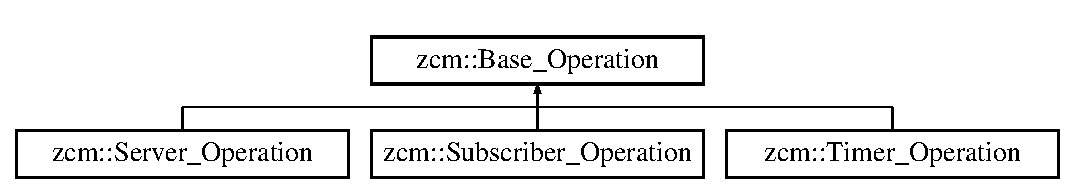
\includegraphics[height=2.000000cm]{classzcm_1_1Base__Operation}
\end{center}
\end{figure}
\subsection*{Public Member Functions}
\begin{DoxyCompactItemize}
\item 
\hyperlink{classzcm_1_1Base__Operation_a87b61a8e801615935c649bae05b9c88e}{Base\-\_\-\-Operation} (std\-::string \hyperlink{classzcm_1_1Base__Operation_a2e2192550818d8f063fc7b2c76c5e21c}{name}, unsigned int \hyperlink{classzcm_1_1Base__Operation_a38af3bcc2578ef215772d595bf3fa358}{priority})
\begin{DoxyCompactList}\small\item\em Construct a base operation. \end{DoxyCompactList}\item 
std\-::string \hyperlink{classzcm_1_1Base__Operation_a46b6a3f23e18bc35425ec2dab80c849f}{get\-\_\-name} ()
\begin{DoxyCompactList}\small\item\em Return the operation name. \end{DoxyCompactList}\item 
unsigned int \hyperlink{classzcm_1_1Base__Operation_a3b15b35c31ed173d2abb193e9fba32ef}{get\-\_\-priority} () const 
\begin{DoxyCompactList}\small\item\em Return the operation priority. \end{DoxyCompactList}\item 
virtual void \hyperlink{classzcm_1_1Base__Operation_a58cb533edd6e6f220d2d1c260fbddca4}{execute} ()
\begin{DoxyCompactList}\small\item\em Virtual execute function overridden by concrete types. \end{DoxyCompactList}\end{DoxyCompactItemize}
\subsection*{Private Attributes}
\begin{DoxyCompactItemize}
\item 
std\-::string \hyperlink{classzcm_1_1Base__Operation_a2e2192550818d8f063fc7b2c76c5e21c}{name}
\begin{DoxyCompactList}\small\item\em Name of the Operation. \end{DoxyCompactList}\item 
unsigned int \hyperlink{classzcm_1_1Base__Operation_a38af3bcc2578ef215772d595bf3fa358}{priority}
\begin{DoxyCompactList}\small\item\em Priority of the Operation. \end{DoxyCompactList}\end{DoxyCompactItemize}


\subsection{Detailed Description}
Base Operation class. 

\subsection{Constructor \& Destructor Documentation}
\hypertarget{classzcm_1_1Base__Operation_a87b61a8e801615935c649bae05b9c88e}{\index{zcm\-::\-Base\-\_\-\-Operation@{zcm\-::\-Base\-\_\-\-Operation}!Base\-\_\-\-Operation@{Base\-\_\-\-Operation}}
\index{Base\-\_\-\-Operation@{Base\-\_\-\-Operation}!zcm::Base_Operation@{zcm\-::\-Base\-\_\-\-Operation}}
\subsubsection[{Base\-\_\-\-Operation}]{\setlength{\rightskip}{0pt plus 5cm}zcm\-::\-Base\-\_\-\-Operation\-::\-Base\-\_\-\-Operation (
\begin{DoxyParamCaption}
\item[{std\-::string}]{name, }
\item[{unsigned int}]{priority}
\end{DoxyParamCaption}
)\hspace{0.3cm}{\ttfamily [inline]}}}\label{classzcm_1_1Base__Operation_a87b61a8e801615935c649bae05b9c88e}


Construct a base operation. 


\begin{DoxyParams}[1]{Parameters}
\mbox{\tt in}  & {\em name} & Name of the operation \\
\hline
\mbox{\tt in}  & {\em priority} & Priority of the operation \\
\hline
\end{DoxyParams}


\subsection{Member Function Documentation}
\hypertarget{classzcm_1_1Base__Operation_a58cb533edd6e6f220d2d1c260fbddca4}{\index{zcm\-::\-Base\-\_\-\-Operation@{zcm\-::\-Base\-\_\-\-Operation}!execute@{execute}}
\index{execute@{execute}!zcm::Base_Operation@{zcm\-::\-Base\-\_\-\-Operation}}
\subsubsection[{execute}]{\setlength{\rightskip}{0pt plus 5cm}virtual void zcm\-::\-Base\-\_\-\-Operation\-::execute (
\begin{DoxyParamCaption}
{}
\end{DoxyParamCaption}
)\hspace{0.3cm}{\ttfamily [inline]}, {\ttfamily [virtual]}}}\label{classzcm_1_1Base__Operation_a58cb533edd6e6f220d2d1c260fbddca4}


Virtual execute function overridden by concrete types. 



Reimplemented in \hyperlink{classzcm_1_1Server__Operation_acd6b89c42aad3df5dc78674770326498}{zcm\-::\-Server\-\_\-\-Operation}, \hyperlink{classzcm_1_1Subscriber__Operation_a2677079c7f3dd85cfc548427c1c101e6}{zcm\-::\-Subscriber\-\_\-\-Operation}, and \hyperlink{classzcm_1_1Timer__Operation_a3693312c4d4d106d0894bb35094efda7}{zcm\-::\-Timer\-\_\-\-Operation}.

\hypertarget{classzcm_1_1Base__Operation_a46b6a3f23e18bc35425ec2dab80c849f}{\index{zcm\-::\-Base\-\_\-\-Operation@{zcm\-::\-Base\-\_\-\-Operation}!get\-\_\-name@{get\-\_\-name}}
\index{get\-\_\-name@{get\-\_\-name}!zcm::Base_Operation@{zcm\-::\-Base\-\_\-\-Operation}}
\subsubsection[{get\-\_\-name}]{\setlength{\rightskip}{0pt plus 5cm}std\-::string zcm\-::\-Base\-\_\-\-Operation\-::get\-\_\-name (
\begin{DoxyParamCaption}
{}
\end{DoxyParamCaption}
)}}\label{classzcm_1_1Base__Operation_a46b6a3f23e18bc35425ec2dab80c849f}


Return the operation name. 

\begin{DoxyReturn}{Returns}
Name of the operation 
\end{DoxyReturn}
\hypertarget{classzcm_1_1Base__Operation_a3b15b35c31ed173d2abb193e9fba32ef}{\index{zcm\-::\-Base\-\_\-\-Operation@{zcm\-::\-Base\-\_\-\-Operation}!get\-\_\-priority@{get\-\_\-priority}}
\index{get\-\_\-priority@{get\-\_\-priority}!zcm::Base_Operation@{zcm\-::\-Base\-\_\-\-Operation}}
\subsubsection[{get\-\_\-priority}]{\setlength{\rightskip}{0pt plus 5cm}unsigned int zcm\-::\-Base\-\_\-\-Operation\-::get\-\_\-priority (
\begin{DoxyParamCaption}
{}
\end{DoxyParamCaption}
) const}}\label{classzcm_1_1Base__Operation_a3b15b35c31ed173d2abb193e9fba32ef}


Return the operation priority. 

\begin{DoxyReturn}{Returns}
Priority of the operation 
\end{DoxyReturn}


\subsection{Member Data Documentation}
\hypertarget{classzcm_1_1Base__Operation_a2e2192550818d8f063fc7b2c76c5e21c}{\index{zcm\-::\-Base\-\_\-\-Operation@{zcm\-::\-Base\-\_\-\-Operation}!name@{name}}
\index{name@{name}!zcm::Base_Operation@{zcm\-::\-Base\-\_\-\-Operation}}
\subsubsection[{name}]{\setlength{\rightskip}{0pt plus 5cm}std\-::string zcm\-::\-Base\-\_\-\-Operation\-::name\hspace{0.3cm}{\ttfamily [private]}}}\label{classzcm_1_1Base__Operation_a2e2192550818d8f063fc7b2c76c5e21c}


Name of the Operation. 

\hypertarget{classzcm_1_1Base__Operation_a38af3bcc2578ef215772d595bf3fa358}{\index{zcm\-::\-Base\-\_\-\-Operation@{zcm\-::\-Base\-\_\-\-Operation}!priority@{priority}}
\index{priority@{priority}!zcm::Base_Operation@{zcm\-::\-Base\-\_\-\-Operation}}
\subsubsection[{priority}]{\setlength{\rightskip}{0pt plus 5cm}unsigned int zcm\-::\-Base\-\_\-\-Operation\-::priority\hspace{0.3cm}{\ttfamily [private]}}}\label{classzcm_1_1Base__Operation_a38af3bcc2578ef215772d595bf3fa358}


Priority of the Operation. 



The documentation for this class was generated from the following files\-:\begin{DoxyCompactItemize}
\item 
/home/kelsier/\-Git\-Hub/zcm/include/\hyperlink{operation__types_8hpp}{operation\-\_\-types.\-hpp}\item 
/home/kelsier/\-Git\-Hub/zcm/src/\hyperlink{operation__types_8cpp}{operation\-\_\-types.\-cpp}\end{DoxyCompactItemize}

\hypertarget{structJson_1_1BuiltStyledStreamWriter}{}\section{Json\+:\+:Built\+Styled\+Stream\+Writer Struct Reference}
\label{structJson_1_1BuiltStyledStreamWriter}\index{Json\+::\+Built\+Styled\+Stream\+Writer@{Json\+::\+Built\+Styled\+Stream\+Writer}}
Inheritance diagram for Json\+:\+:Built\+Styled\+Stream\+Writer\+:\begin{figure}[H]
\begin{center}
\leavevmode
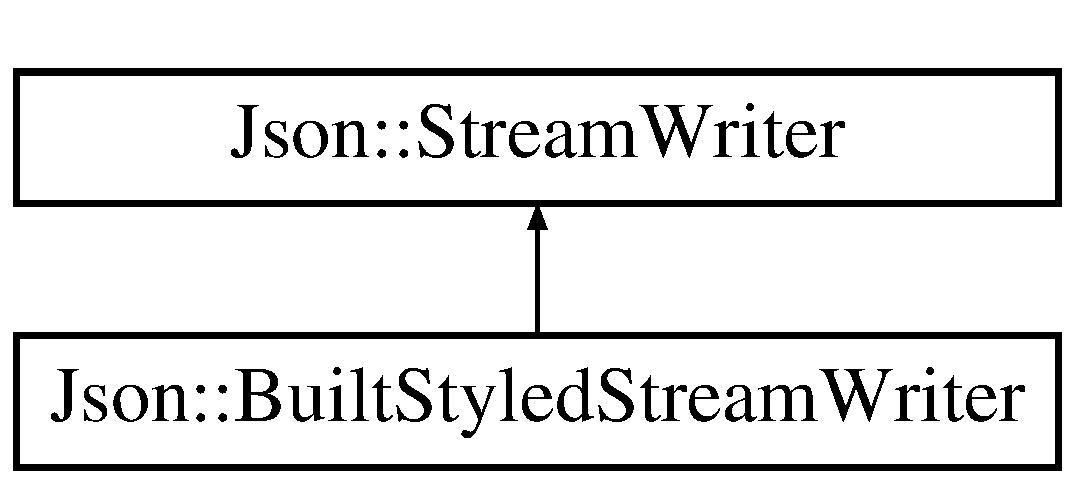
\includegraphics[height=2.000000cm]{structJson_1_1BuiltStyledStreamWriter}
\end{center}
\end{figure}
\subsection*{Public Member Functions}
\begin{DoxyCompactItemize}
\item 
\hyperlink{structJson_1_1BuiltStyledStreamWriter_adf11b7d1ee3c68d096b7c662ee85948e}{Built\+Styled\+Stream\+Writer} (\hyperlink{json_8hpp_a1e723f95759de062585bc4a8fd3fa4be}{J\+S\+O\+N\+C\+P\+P\+\_\+\+S\+T\+R\+I\+NG} const \&indentation, \hyperlink{structJson_1_1CommentStyle_a51fc08f3518fd81eba12f340d19a3d0c}{Comment\+Style\+::\+Enum} cs, \hyperlink{json_8hpp_a1e723f95759de062585bc4a8fd3fa4be}{J\+S\+O\+N\+C\+P\+P\+\_\+\+S\+T\+R\+I\+NG} const \&colon\+Symbol, \hyperlink{json_8hpp_a1e723f95759de062585bc4a8fd3fa4be}{J\+S\+O\+N\+C\+P\+P\+\_\+\+S\+T\+R\+I\+NG} const \&null\+Symbol, \hyperlink{json_8hpp_a1e723f95759de062585bc4a8fd3fa4be}{J\+S\+O\+N\+C\+P\+P\+\_\+\+S\+T\+R\+I\+NG} const \&ending\+Line\+Feed\+Symbol, bool use\+Special\+Floats, unsigned int precision)
\item 
int \hyperlink{structJson_1_1BuiltStyledStreamWriter_a823cdb1afabb6b0d5f39bcd5a6a6f747}{write} (\hyperlink{classJson_1_1Value}{Value} const \&root, \hyperlink{json_8hpp_a37a25be5fca174927780caeb280094ce}{J\+S\+O\+N\+C\+P\+P\+\_\+\+O\+S\+T\+R\+E\+AM} $\ast$sout) \hyperlink{json_8hpp_a824d6199c91488107e443226fa6022c5}{J\+S\+O\+N\+C\+P\+P\+\_\+\+O\+V\+E\+R\+R\+I\+DE}
\begin{DoxyCompactList}\small\item\em Write \hyperlink{classJson_1_1Value}{Value} into document as configured in sub-\/class. \end{DoxyCompactList}\end{DoxyCompactItemize}
\subsection*{Protected Attributes}
\begin{DoxyCompactItemize}
\item 
\hyperlink{json_8hpp_a37a25be5fca174927780caeb280094ce}{J\+S\+O\+N\+C\+P\+P\+\_\+\+O\+S\+T\+R\+E\+AM} $\ast$ \hyperlink{classJson_1_1StreamWriter_a4f5603d4228a9fa46a42cb44e5234d9b}{sout\+\_\+}
\end{DoxyCompactItemize}
\subsection*{Private Types}
\begin{DoxyCompactItemize}
\item 
typedef std\+::vector$<$ \hyperlink{json_8hpp_a1e723f95759de062585bc4a8fd3fa4be}{J\+S\+O\+N\+C\+P\+P\+\_\+\+S\+T\+R\+I\+NG} $>$ \hyperlink{structJson_1_1BuiltStyledStreamWriter_a63196b38400e5ce452f65ce856d47b6f}{Child\+Values}
\end{DoxyCompactItemize}
\subsection*{Private Member Functions}
\begin{DoxyCompactItemize}
\item 
void \hyperlink{structJson_1_1BuiltStyledStreamWriter_a7c9da861861e570a51b45f270c9ff150}{write\+Value} (\hyperlink{classJson_1_1Value}{Value} const \&value)
\item 
void \hyperlink{structJson_1_1BuiltStyledStreamWriter_acd20e9274bbcf7876ef3af2e7d23a31f}{write\+Array\+Value} (\hyperlink{classJson_1_1Value}{Value} const \&value)
\item 
bool \hyperlink{structJson_1_1BuiltStyledStreamWriter_af423fd33b3d580506ea3efc53b05a077}{is\+Multine\+Array} (\hyperlink{classJson_1_1Value}{Value} const \&value)
\item 
void \hyperlink{structJson_1_1BuiltStyledStreamWriter_a91e8535508412eea04d77c0cafdf15aa}{push\+Value} (\hyperlink{json_8hpp_a1e723f95759de062585bc4a8fd3fa4be}{J\+S\+O\+N\+C\+P\+P\+\_\+\+S\+T\+R\+I\+NG} const \&value)
\item 
void \hyperlink{structJson_1_1BuiltStyledStreamWriter_a2b38a3714d415c4bd3b4812897130f3d}{write\+Indent} ()
\item 
void \hyperlink{structJson_1_1BuiltStyledStreamWriter_a6e80e1a0d5f64df2ec48c3c3b1284990}{write\+With\+Indent} (\hyperlink{json_8hpp_a1e723f95759de062585bc4a8fd3fa4be}{J\+S\+O\+N\+C\+P\+P\+\_\+\+S\+T\+R\+I\+NG} const \&value)
\item 
void \hyperlink{structJson_1_1BuiltStyledStreamWriter_a73e09692a2cfbd6e67836b060dc34a9f}{indent} ()
\item 
void \hyperlink{structJson_1_1BuiltStyledStreamWriter_a0da6c6f603e00c8c6e38af553edd8c55}{unindent} ()
\item 
void \hyperlink{structJson_1_1BuiltStyledStreamWriter_a32c4afca4e08fba79bb0a80a8010283a}{write\+Comment\+Before\+Value} (\hyperlink{classJson_1_1Value}{Value} const \&root)
\item 
void \hyperlink{structJson_1_1BuiltStyledStreamWriter_a89625b134fce0255263ca40e6125742b}{write\+Comment\+After\+Value\+On\+Same\+Line} (\hyperlink{classJson_1_1Value}{Value} const \&root)
\end{DoxyCompactItemize}
\subsection*{Static Private Member Functions}
\begin{DoxyCompactItemize}
\item 
static bool \hyperlink{structJson_1_1BuiltStyledStreamWriter_a457c2f3c1e8c952caeb60e52477d0c9a}{has\+Comment\+For\+Value} (const \hyperlink{classJson_1_1Value}{Value} \&value)
\end{DoxyCompactItemize}
\subsection*{Private Attributes}
\begin{DoxyCompactItemize}
\item 
\hyperlink{structJson_1_1BuiltStyledStreamWriter_a63196b38400e5ce452f65ce856d47b6f}{Child\+Values} \hyperlink{structJson_1_1BuiltStyledStreamWriter_a47d562d7874c5b1e68995bd62f575792}{child\+Values\+\_\+}
\item 
\hyperlink{json_8hpp_a1e723f95759de062585bc4a8fd3fa4be}{J\+S\+O\+N\+C\+P\+P\+\_\+\+S\+T\+R\+I\+NG} \hyperlink{structJson_1_1BuiltStyledStreamWriter_a0f8115a4fb474ab0e9de25f10e5ca09a}{indent\+String\+\_\+}
\item 
unsigned int \hyperlink{structJson_1_1BuiltStyledStreamWriter_a06a51521ccae20397f52fe3036edc602}{right\+Margin\+\_\+}
\item 
\hyperlink{json_8hpp_a1e723f95759de062585bc4a8fd3fa4be}{J\+S\+O\+N\+C\+P\+P\+\_\+\+S\+T\+R\+I\+NG} \hyperlink{structJson_1_1BuiltStyledStreamWriter_aaa4cbad91428ceca37cbabfc2a17a92d}{indentation\+\_\+}
\item 
\hyperlink{structJson_1_1CommentStyle_a51fc08f3518fd81eba12f340d19a3d0c}{Comment\+Style\+::\+Enum} \hyperlink{structJson_1_1BuiltStyledStreamWriter_a89a9c76c7531143b52785861ba21c1d4}{cs\+\_\+}
\item 
\hyperlink{json_8hpp_a1e723f95759de062585bc4a8fd3fa4be}{J\+S\+O\+N\+C\+P\+P\+\_\+\+S\+T\+R\+I\+NG} \hyperlink{structJson_1_1BuiltStyledStreamWriter_a9f10991ddef9b77d0b580e24e71483c6}{colon\+Symbol\+\_\+}
\item 
\hyperlink{json_8hpp_a1e723f95759de062585bc4a8fd3fa4be}{J\+S\+O\+N\+C\+P\+P\+\_\+\+S\+T\+R\+I\+NG} \hyperlink{structJson_1_1BuiltStyledStreamWriter_a6ccceadf4b1286a519a175cb59cb61d5}{null\+Symbol\+\_\+}
\item 
\hyperlink{json_8hpp_a1e723f95759de062585bc4a8fd3fa4be}{J\+S\+O\+N\+C\+P\+P\+\_\+\+S\+T\+R\+I\+NG} \hyperlink{structJson_1_1BuiltStyledStreamWriter_a5e61a9a4b2af52b98900286c843b86f7}{ending\+Line\+Feed\+Symbol\+\_\+}
\item 
bool \hyperlink{structJson_1_1BuiltStyledStreamWriter_abed9cc31da503b48798e7cea68c42e16}{add\+Child\+Values\+\_\+}\+: 1
\item 
bool \hyperlink{structJson_1_1BuiltStyledStreamWriter_a6aa0ad023e623f600103631a6bca6d10}{indented\+\_\+}\+: 1
\item 
bool \hyperlink{structJson_1_1BuiltStyledStreamWriter_a6f1b8694b4eb17ab8c34f6d6dd8c8a4a}{use\+Special\+Floats\+\_\+}\+: 1
\item 
unsigned int \hyperlink{structJson_1_1BuiltStyledStreamWriter_a6373d8d0ae4741b64e3904e4db0eef46}{precision\+\_\+}
\end{DoxyCompactItemize}


\subsection{Member Typedef Documentation}
\index{Json\+::\+Built\+Styled\+Stream\+Writer@{Json\+::\+Built\+Styled\+Stream\+Writer}!Child\+Values@{Child\+Values}}
\index{Child\+Values@{Child\+Values}!Json\+::\+Built\+Styled\+Stream\+Writer@{Json\+::\+Built\+Styled\+Stream\+Writer}}
\subsubsection[{\texorpdfstring{Child\+Values}{ChildValues}}]{\setlength{\rightskip}{0pt plus 5cm}typedef std\+::vector$<${\bf J\+S\+O\+N\+C\+P\+P\+\_\+\+S\+T\+R\+I\+NG}$>$ {\bf Json\+::\+Built\+Styled\+Stream\+Writer\+::\+Child\+Values}\hspace{0.3cm}{\ttfamily [private]}}\hypertarget{structJson_1_1BuiltStyledStreamWriter_a63196b38400e5ce452f65ce856d47b6f}{}\label{structJson_1_1BuiltStyledStreamWriter_a63196b38400e5ce452f65ce856d47b6f}


\subsection{Constructor \& Destructor Documentation}
\index{Json\+::\+Built\+Styled\+Stream\+Writer@{Json\+::\+Built\+Styled\+Stream\+Writer}!Built\+Styled\+Stream\+Writer@{Built\+Styled\+Stream\+Writer}}
\index{Built\+Styled\+Stream\+Writer@{Built\+Styled\+Stream\+Writer}!Json\+::\+Built\+Styled\+Stream\+Writer@{Json\+::\+Built\+Styled\+Stream\+Writer}}
\subsubsection[{\texorpdfstring{Built\+Styled\+Stream\+Writer(\+J\+S\+O\+N\+C\+P\+P\+\_\+\+S\+T\+R\+I\+N\+G const \&indentation, Comment\+Style\+::\+Enum cs, J\+S\+O\+N\+C\+P\+P\+\_\+\+S\+T\+R\+I\+N\+G const \&colon\+Symbol, J\+S\+O\+N\+C\+P\+P\+\_\+\+S\+T\+R\+I\+N\+G const \&null\+Symbol, J\+S\+O\+N\+C\+P\+P\+\_\+\+S\+T\+R\+I\+N\+G const \&ending\+Line\+Feed\+Symbol, bool use\+Special\+Floats, unsigned int precision)}{BuiltStyledStreamWriter(JSONCPP_STRING const &indentation, CommentStyle::Enum cs, JSONCPP_STRING const &colonSymbol, JSONCPP_STRING const &nullSymbol, JSONCPP_STRING const &endingLineFeedSymbol, bool useSpecialFloats, unsigned int precision)}}]{\setlength{\rightskip}{0pt plus 5cm}Json\+::\+Built\+Styled\+Stream\+Writer\+::\+Built\+Styled\+Stream\+Writer (
\begin{DoxyParamCaption}
\item[{{\bf J\+S\+O\+N\+C\+P\+P\+\_\+\+S\+T\+R\+I\+NG} const \&}]{indentation, }
\item[{{\bf Comment\+Style\+::\+Enum}}]{cs, }
\item[{{\bf J\+S\+O\+N\+C\+P\+P\+\_\+\+S\+T\+R\+I\+NG} const \&}]{colon\+Symbol, }
\item[{{\bf J\+S\+O\+N\+C\+P\+P\+\_\+\+S\+T\+R\+I\+NG} const \&}]{null\+Symbol, }
\item[{{\bf J\+S\+O\+N\+C\+P\+P\+\_\+\+S\+T\+R\+I\+NG} const \&}]{ending\+Line\+Feed\+Symbol, }
\item[{bool}]{use\+Special\+Floats, }
\item[{unsigned int}]{precision}
\end{DoxyParamCaption}
)}\hypertarget{structJson_1_1BuiltStyledStreamWriter_adf11b7d1ee3c68d096b7c662ee85948e}{}\label{structJson_1_1BuiltStyledStreamWriter_adf11b7d1ee3c68d096b7c662ee85948e}


\subsection{Member Function Documentation}
\index{Json\+::\+Built\+Styled\+Stream\+Writer@{Json\+::\+Built\+Styled\+Stream\+Writer}!has\+Comment\+For\+Value@{has\+Comment\+For\+Value}}
\index{has\+Comment\+For\+Value@{has\+Comment\+For\+Value}!Json\+::\+Built\+Styled\+Stream\+Writer@{Json\+::\+Built\+Styled\+Stream\+Writer}}
\subsubsection[{\texorpdfstring{has\+Comment\+For\+Value(const Value \&value)}{hasCommentForValue(const Value &value)}}]{\setlength{\rightskip}{0pt plus 5cm}bool Json\+::\+Built\+Styled\+Stream\+Writer\+::has\+Comment\+For\+Value (
\begin{DoxyParamCaption}
\item[{const {\bf Value} \&}]{value}
\end{DoxyParamCaption}
)\hspace{0.3cm}{\ttfamily [static]}, {\ttfamily [private]}}\hypertarget{structJson_1_1BuiltStyledStreamWriter_a457c2f3c1e8c952caeb60e52477d0c9a}{}\label{structJson_1_1BuiltStyledStreamWriter_a457c2f3c1e8c952caeb60e52477d0c9a}
\index{Json\+::\+Built\+Styled\+Stream\+Writer@{Json\+::\+Built\+Styled\+Stream\+Writer}!indent@{indent}}
\index{indent@{indent}!Json\+::\+Built\+Styled\+Stream\+Writer@{Json\+::\+Built\+Styled\+Stream\+Writer}}
\subsubsection[{\texorpdfstring{indent()}{indent()}}]{\setlength{\rightskip}{0pt plus 5cm}void Json\+::\+Built\+Styled\+Stream\+Writer\+::indent (
\begin{DoxyParamCaption}
{}
\end{DoxyParamCaption}
)\hspace{0.3cm}{\ttfamily [private]}}\hypertarget{structJson_1_1BuiltStyledStreamWriter_a73e09692a2cfbd6e67836b060dc34a9f}{}\label{structJson_1_1BuiltStyledStreamWriter_a73e09692a2cfbd6e67836b060dc34a9f}
\index{Json\+::\+Built\+Styled\+Stream\+Writer@{Json\+::\+Built\+Styled\+Stream\+Writer}!is\+Multine\+Array@{is\+Multine\+Array}}
\index{is\+Multine\+Array@{is\+Multine\+Array}!Json\+::\+Built\+Styled\+Stream\+Writer@{Json\+::\+Built\+Styled\+Stream\+Writer}}
\subsubsection[{\texorpdfstring{is\+Multine\+Array(\+Value const \&value)}{isMultineArray(Value const &value)}}]{\setlength{\rightskip}{0pt plus 5cm}bool Json\+::\+Built\+Styled\+Stream\+Writer\+::is\+Multine\+Array (
\begin{DoxyParamCaption}
\item[{{\bf Value} const \&}]{value}
\end{DoxyParamCaption}
)\hspace{0.3cm}{\ttfamily [private]}}\hypertarget{structJson_1_1BuiltStyledStreamWriter_af423fd33b3d580506ea3efc53b05a077}{}\label{structJson_1_1BuiltStyledStreamWriter_af423fd33b3d580506ea3efc53b05a077}
\index{Json\+::\+Built\+Styled\+Stream\+Writer@{Json\+::\+Built\+Styled\+Stream\+Writer}!push\+Value@{push\+Value}}
\index{push\+Value@{push\+Value}!Json\+::\+Built\+Styled\+Stream\+Writer@{Json\+::\+Built\+Styled\+Stream\+Writer}}
\subsubsection[{\texorpdfstring{push\+Value(\+J\+S\+O\+N\+C\+P\+P\+\_\+\+S\+T\+R\+I\+N\+G const \&value)}{pushValue(JSONCPP_STRING const &value)}}]{\setlength{\rightskip}{0pt plus 5cm}void Json\+::\+Built\+Styled\+Stream\+Writer\+::push\+Value (
\begin{DoxyParamCaption}
\item[{{\bf J\+S\+O\+N\+C\+P\+P\+\_\+\+S\+T\+R\+I\+NG} const \&}]{value}
\end{DoxyParamCaption}
)\hspace{0.3cm}{\ttfamily [private]}}\hypertarget{structJson_1_1BuiltStyledStreamWriter_a91e8535508412eea04d77c0cafdf15aa}{}\label{structJson_1_1BuiltStyledStreamWriter_a91e8535508412eea04d77c0cafdf15aa}
\index{Json\+::\+Built\+Styled\+Stream\+Writer@{Json\+::\+Built\+Styled\+Stream\+Writer}!unindent@{unindent}}
\index{unindent@{unindent}!Json\+::\+Built\+Styled\+Stream\+Writer@{Json\+::\+Built\+Styled\+Stream\+Writer}}
\subsubsection[{\texorpdfstring{unindent()}{unindent()}}]{\setlength{\rightskip}{0pt plus 5cm}void Json\+::\+Built\+Styled\+Stream\+Writer\+::unindent (
\begin{DoxyParamCaption}
{}
\end{DoxyParamCaption}
)\hspace{0.3cm}{\ttfamily [private]}}\hypertarget{structJson_1_1BuiltStyledStreamWriter_a0da6c6f603e00c8c6e38af553edd8c55}{}\label{structJson_1_1BuiltStyledStreamWriter_a0da6c6f603e00c8c6e38af553edd8c55}
\index{Json\+::\+Built\+Styled\+Stream\+Writer@{Json\+::\+Built\+Styled\+Stream\+Writer}!write@{write}}
\index{write@{write}!Json\+::\+Built\+Styled\+Stream\+Writer@{Json\+::\+Built\+Styled\+Stream\+Writer}}
\subsubsection[{\texorpdfstring{write(\+Value const \&root, J\+S\+O\+N\+C\+P\+P\+\_\+\+O\+S\+T\+R\+E\+A\+M $\ast$sout) J\+S\+O\+N\+C\+P\+P\+\_\+\+O\+V\+E\+R\+R\+I\+DE}{write(Value const &root, JSONCPP_OSTREAM *sout) JSONCPP_OVERRIDE}}]{\setlength{\rightskip}{0pt plus 5cm}int Json\+::\+Built\+Styled\+Stream\+Writer\+::write (
\begin{DoxyParamCaption}
\item[{{\bf Value} const \&}]{root, }
\item[{{\bf J\+S\+O\+N\+C\+P\+P\+\_\+\+O\+S\+T\+R\+E\+AM} $\ast$}]{sout}
\end{DoxyParamCaption}
)\hspace{0.3cm}{\ttfamily [virtual]}}\hypertarget{structJson_1_1BuiltStyledStreamWriter_a823cdb1afabb6b0d5f39bcd5a6a6f747}{}\label{structJson_1_1BuiltStyledStreamWriter_a823cdb1afabb6b0d5f39bcd5a6a6f747}


Write \hyperlink{classJson_1_1Value}{Value} into document as configured in sub-\/class. 

Do not take ownership of sout, but maintain a reference during function. \begin{DoxyPrecond}{Precondition}
sout != N\+U\+LL 
\end{DoxyPrecond}
\begin{DoxyReturn}{Returns}
zero on success (For now, we always return zero, so check the stream instead.) 
\end{DoxyReturn}

\begin{DoxyExceptions}{Exceptions}
{\em std\+::exception} & possibly, depending on configuration \\
\hline
\end{DoxyExceptions}


Implements \hyperlink{classJson_1_1StreamWriter_a84278bad0c9a9fc587bc2a97c5bb5993}{Json\+::\+Stream\+Writer}.

\index{Json\+::\+Built\+Styled\+Stream\+Writer@{Json\+::\+Built\+Styled\+Stream\+Writer}!write\+Array\+Value@{write\+Array\+Value}}
\index{write\+Array\+Value@{write\+Array\+Value}!Json\+::\+Built\+Styled\+Stream\+Writer@{Json\+::\+Built\+Styled\+Stream\+Writer}}
\subsubsection[{\texorpdfstring{write\+Array\+Value(\+Value const \&value)}{writeArrayValue(Value const &value)}}]{\setlength{\rightskip}{0pt plus 5cm}void Json\+::\+Built\+Styled\+Stream\+Writer\+::write\+Array\+Value (
\begin{DoxyParamCaption}
\item[{{\bf Value} const \&}]{value}
\end{DoxyParamCaption}
)\hspace{0.3cm}{\ttfamily [private]}}\hypertarget{structJson_1_1BuiltStyledStreamWriter_acd20e9274bbcf7876ef3af2e7d23a31f}{}\label{structJson_1_1BuiltStyledStreamWriter_acd20e9274bbcf7876ef3af2e7d23a31f}
\index{Json\+::\+Built\+Styled\+Stream\+Writer@{Json\+::\+Built\+Styled\+Stream\+Writer}!write\+Comment\+After\+Value\+On\+Same\+Line@{write\+Comment\+After\+Value\+On\+Same\+Line}}
\index{write\+Comment\+After\+Value\+On\+Same\+Line@{write\+Comment\+After\+Value\+On\+Same\+Line}!Json\+::\+Built\+Styled\+Stream\+Writer@{Json\+::\+Built\+Styled\+Stream\+Writer}}
\subsubsection[{\texorpdfstring{write\+Comment\+After\+Value\+On\+Same\+Line(\+Value const \&root)}{writeCommentAfterValueOnSameLine(Value const &root)}}]{\setlength{\rightskip}{0pt plus 5cm}void Json\+::\+Built\+Styled\+Stream\+Writer\+::write\+Comment\+After\+Value\+On\+Same\+Line (
\begin{DoxyParamCaption}
\item[{{\bf Value} const \&}]{root}
\end{DoxyParamCaption}
)\hspace{0.3cm}{\ttfamily [private]}}\hypertarget{structJson_1_1BuiltStyledStreamWriter_a89625b134fce0255263ca40e6125742b}{}\label{structJson_1_1BuiltStyledStreamWriter_a89625b134fce0255263ca40e6125742b}
\index{Json\+::\+Built\+Styled\+Stream\+Writer@{Json\+::\+Built\+Styled\+Stream\+Writer}!write\+Comment\+Before\+Value@{write\+Comment\+Before\+Value}}
\index{write\+Comment\+Before\+Value@{write\+Comment\+Before\+Value}!Json\+::\+Built\+Styled\+Stream\+Writer@{Json\+::\+Built\+Styled\+Stream\+Writer}}
\subsubsection[{\texorpdfstring{write\+Comment\+Before\+Value(\+Value const \&root)}{writeCommentBeforeValue(Value const &root)}}]{\setlength{\rightskip}{0pt plus 5cm}void Json\+::\+Built\+Styled\+Stream\+Writer\+::write\+Comment\+Before\+Value (
\begin{DoxyParamCaption}
\item[{{\bf Value} const \&}]{root}
\end{DoxyParamCaption}
)\hspace{0.3cm}{\ttfamily [private]}}\hypertarget{structJson_1_1BuiltStyledStreamWriter_a32c4afca4e08fba79bb0a80a8010283a}{}\label{structJson_1_1BuiltStyledStreamWriter_a32c4afca4e08fba79bb0a80a8010283a}
\index{Json\+::\+Built\+Styled\+Stream\+Writer@{Json\+::\+Built\+Styled\+Stream\+Writer}!write\+Indent@{write\+Indent}}
\index{write\+Indent@{write\+Indent}!Json\+::\+Built\+Styled\+Stream\+Writer@{Json\+::\+Built\+Styled\+Stream\+Writer}}
\subsubsection[{\texorpdfstring{write\+Indent()}{writeIndent()}}]{\setlength{\rightskip}{0pt plus 5cm}void Json\+::\+Built\+Styled\+Stream\+Writer\+::write\+Indent (
\begin{DoxyParamCaption}
{}
\end{DoxyParamCaption}
)\hspace{0.3cm}{\ttfamily [private]}}\hypertarget{structJson_1_1BuiltStyledStreamWriter_a2b38a3714d415c4bd3b4812897130f3d}{}\label{structJson_1_1BuiltStyledStreamWriter_a2b38a3714d415c4bd3b4812897130f3d}
\index{Json\+::\+Built\+Styled\+Stream\+Writer@{Json\+::\+Built\+Styled\+Stream\+Writer}!write\+Value@{write\+Value}}
\index{write\+Value@{write\+Value}!Json\+::\+Built\+Styled\+Stream\+Writer@{Json\+::\+Built\+Styled\+Stream\+Writer}}
\subsubsection[{\texorpdfstring{write\+Value(\+Value const \&value)}{writeValue(Value const &value)}}]{\setlength{\rightskip}{0pt plus 5cm}void Json\+::\+Built\+Styled\+Stream\+Writer\+::write\+Value (
\begin{DoxyParamCaption}
\item[{{\bf Value} const \&}]{value}
\end{DoxyParamCaption}
)\hspace{0.3cm}{\ttfamily [private]}}\hypertarget{structJson_1_1BuiltStyledStreamWriter_a7c9da861861e570a51b45f270c9ff150}{}\label{structJson_1_1BuiltStyledStreamWriter_a7c9da861861e570a51b45f270c9ff150}
\index{Json\+::\+Built\+Styled\+Stream\+Writer@{Json\+::\+Built\+Styled\+Stream\+Writer}!write\+With\+Indent@{write\+With\+Indent}}
\index{write\+With\+Indent@{write\+With\+Indent}!Json\+::\+Built\+Styled\+Stream\+Writer@{Json\+::\+Built\+Styled\+Stream\+Writer}}
\subsubsection[{\texorpdfstring{write\+With\+Indent(\+J\+S\+O\+N\+C\+P\+P\+\_\+\+S\+T\+R\+I\+N\+G const \&value)}{writeWithIndent(JSONCPP_STRING const &value)}}]{\setlength{\rightskip}{0pt plus 5cm}void Json\+::\+Built\+Styled\+Stream\+Writer\+::write\+With\+Indent (
\begin{DoxyParamCaption}
\item[{{\bf J\+S\+O\+N\+C\+P\+P\+\_\+\+S\+T\+R\+I\+NG} const \&}]{value}
\end{DoxyParamCaption}
)\hspace{0.3cm}{\ttfamily [private]}}\hypertarget{structJson_1_1BuiltStyledStreamWriter_a6e80e1a0d5f64df2ec48c3c3b1284990}{}\label{structJson_1_1BuiltStyledStreamWriter_a6e80e1a0d5f64df2ec48c3c3b1284990}


\subsection{Member Data Documentation}
\index{Json\+::\+Built\+Styled\+Stream\+Writer@{Json\+::\+Built\+Styled\+Stream\+Writer}!add\+Child\+Values\+\_\+@{add\+Child\+Values\+\_\+}}
\index{add\+Child\+Values\+\_\+@{add\+Child\+Values\+\_\+}!Json\+::\+Built\+Styled\+Stream\+Writer@{Json\+::\+Built\+Styled\+Stream\+Writer}}
\subsubsection[{\texorpdfstring{add\+Child\+Values\+\_\+}{addChildValues_}}]{\setlength{\rightskip}{0pt plus 5cm}bool Json\+::\+Built\+Styled\+Stream\+Writer\+::add\+Child\+Values\+\_\+\hspace{0.3cm}{\ttfamily [private]}}\hypertarget{structJson_1_1BuiltStyledStreamWriter_abed9cc31da503b48798e7cea68c42e16}{}\label{structJson_1_1BuiltStyledStreamWriter_abed9cc31da503b48798e7cea68c42e16}
\index{Json\+::\+Built\+Styled\+Stream\+Writer@{Json\+::\+Built\+Styled\+Stream\+Writer}!child\+Values\+\_\+@{child\+Values\+\_\+}}
\index{child\+Values\+\_\+@{child\+Values\+\_\+}!Json\+::\+Built\+Styled\+Stream\+Writer@{Json\+::\+Built\+Styled\+Stream\+Writer}}
\subsubsection[{\texorpdfstring{child\+Values\+\_\+}{childValues_}}]{\setlength{\rightskip}{0pt plus 5cm}{\bf Child\+Values} Json\+::\+Built\+Styled\+Stream\+Writer\+::child\+Values\+\_\+\hspace{0.3cm}{\ttfamily [private]}}\hypertarget{structJson_1_1BuiltStyledStreamWriter_a47d562d7874c5b1e68995bd62f575792}{}\label{structJson_1_1BuiltStyledStreamWriter_a47d562d7874c5b1e68995bd62f575792}
\index{Json\+::\+Built\+Styled\+Stream\+Writer@{Json\+::\+Built\+Styled\+Stream\+Writer}!colon\+Symbol\+\_\+@{colon\+Symbol\+\_\+}}
\index{colon\+Symbol\+\_\+@{colon\+Symbol\+\_\+}!Json\+::\+Built\+Styled\+Stream\+Writer@{Json\+::\+Built\+Styled\+Stream\+Writer}}
\subsubsection[{\texorpdfstring{colon\+Symbol\+\_\+}{colonSymbol_}}]{\setlength{\rightskip}{0pt plus 5cm}{\bf J\+S\+O\+N\+C\+P\+P\+\_\+\+S\+T\+R\+I\+NG} Json\+::\+Built\+Styled\+Stream\+Writer\+::colon\+Symbol\+\_\+\hspace{0.3cm}{\ttfamily [private]}}\hypertarget{structJson_1_1BuiltStyledStreamWriter_a9f10991ddef9b77d0b580e24e71483c6}{}\label{structJson_1_1BuiltStyledStreamWriter_a9f10991ddef9b77d0b580e24e71483c6}
\index{Json\+::\+Built\+Styled\+Stream\+Writer@{Json\+::\+Built\+Styled\+Stream\+Writer}!cs\+\_\+@{cs\+\_\+}}
\index{cs\+\_\+@{cs\+\_\+}!Json\+::\+Built\+Styled\+Stream\+Writer@{Json\+::\+Built\+Styled\+Stream\+Writer}}
\subsubsection[{\texorpdfstring{cs\+\_\+}{cs_}}]{\setlength{\rightskip}{0pt plus 5cm}{\bf Comment\+Style\+::\+Enum} Json\+::\+Built\+Styled\+Stream\+Writer\+::cs\+\_\+\hspace{0.3cm}{\ttfamily [private]}}\hypertarget{structJson_1_1BuiltStyledStreamWriter_a89a9c76c7531143b52785861ba21c1d4}{}\label{structJson_1_1BuiltStyledStreamWriter_a89a9c76c7531143b52785861ba21c1d4}
\index{Json\+::\+Built\+Styled\+Stream\+Writer@{Json\+::\+Built\+Styled\+Stream\+Writer}!ending\+Line\+Feed\+Symbol\+\_\+@{ending\+Line\+Feed\+Symbol\+\_\+}}
\index{ending\+Line\+Feed\+Symbol\+\_\+@{ending\+Line\+Feed\+Symbol\+\_\+}!Json\+::\+Built\+Styled\+Stream\+Writer@{Json\+::\+Built\+Styled\+Stream\+Writer}}
\subsubsection[{\texorpdfstring{ending\+Line\+Feed\+Symbol\+\_\+}{endingLineFeedSymbol_}}]{\setlength{\rightskip}{0pt plus 5cm}{\bf J\+S\+O\+N\+C\+P\+P\+\_\+\+S\+T\+R\+I\+NG} Json\+::\+Built\+Styled\+Stream\+Writer\+::ending\+Line\+Feed\+Symbol\+\_\+\hspace{0.3cm}{\ttfamily [private]}}\hypertarget{structJson_1_1BuiltStyledStreamWriter_a5e61a9a4b2af52b98900286c843b86f7}{}\label{structJson_1_1BuiltStyledStreamWriter_a5e61a9a4b2af52b98900286c843b86f7}
\index{Json\+::\+Built\+Styled\+Stream\+Writer@{Json\+::\+Built\+Styled\+Stream\+Writer}!indentation\+\_\+@{indentation\+\_\+}}
\index{indentation\+\_\+@{indentation\+\_\+}!Json\+::\+Built\+Styled\+Stream\+Writer@{Json\+::\+Built\+Styled\+Stream\+Writer}}
\subsubsection[{\texorpdfstring{indentation\+\_\+}{indentation_}}]{\setlength{\rightskip}{0pt plus 5cm}{\bf J\+S\+O\+N\+C\+P\+P\+\_\+\+S\+T\+R\+I\+NG} Json\+::\+Built\+Styled\+Stream\+Writer\+::indentation\+\_\+\hspace{0.3cm}{\ttfamily [private]}}\hypertarget{structJson_1_1BuiltStyledStreamWriter_aaa4cbad91428ceca37cbabfc2a17a92d}{}\label{structJson_1_1BuiltStyledStreamWriter_aaa4cbad91428ceca37cbabfc2a17a92d}
\index{Json\+::\+Built\+Styled\+Stream\+Writer@{Json\+::\+Built\+Styled\+Stream\+Writer}!indented\+\_\+@{indented\+\_\+}}
\index{indented\+\_\+@{indented\+\_\+}!Json\+::\+Built\+Styled\+Stream\+Writer@{Json\+::\+Built\+Styled\+Stream\+Writer}}
\subsubsection[{\texorpdfstring{indented\+\_\+}{indented_}}]{\setlength{\rightskip}{0pt plus 5cm}bool Json\+::\+Built\+Styled\+Stream\+Writer\+::indented\+\_\+\hspace{0.3cm}{\ttfamily [private]}}\hypertarget{structJson_1_1BuiltStyledStreamWriter_a6aa0ad023e623f600103631a6bca6d10}{}\label{structJson_1_1BuiltStyledStreamWriter_a6aa0ad023e623f600103631a6bca6d10}
\index{Json\+::\+Built\+Styled\+Stream\+Writer@{Json\+::\+Built\+Styled\+Stream\+Writer}!indent\+String\+\_\+@{indent\+String\+\_\+}}
\index{indent\+String\+\_\+@{indent\+String\+\_\+}!Json\+::\+Built\+Styled\+Stream\+Writer@{Json\+::\+Built\+Styled\+Stream\+Writer}}
\subsubsection[{\texorpdfstring{indent\+String\+\_\+}{indentString_}}]{\setlength{\rightskip}{0pt plus 5cm}{\bf J\+S\+O\+N\+C\+P\+P\+\_\+\+S\+T\+R\+I\+NG} Json\+::\+Built\+Styled\+Stream\+Writer\+::indent\+String\+\_\+\hspace{0.3cm}{\ttfamily [private]}}\hypertarget{structJson_1_1BuiltStyledStreamWriter_a0f8115a4fb474ab0e9de25f10e5ca09a}{}\label{structJson_1_1BuiltStyledStreamWriter_a0f8115a4fb474ab0e9de25f10e5ca09a}
\index{Json\+::\+Built\+Styled\+Stream\+Writer@{Json\+::\+Built\+Styled\+Stream\+Writer}!null\+Symbol\+\_\+@{null\+Symbol\+\_\+}}
\index{null\+Symbol\+\_\+@{null\+Symbol\+\_\+}!Json\+::\+Built\+Styled\+Stream\+Writer@{Json\+::\+Built\+Styled\+Stream\+Writer}}
\subsubsection[{\texorpdfstring{null\+Symbol\+\_\+}{nullSymbol_}}]{\setlength{\rightskip}{0pt plus 5cm}{\bf J\+S\+O\+N\+C\+P\+P\+\_\+\+S\+T\+R\+I\+NG} Json\+::\+Built\+Styled\+Stream\+Writer\+::null\+Symbol\+\_\+\hspace{0.3cm}{\ttfamily [private]}}\hypertarget{structJson_1_1BuiltStyledStreamWriter_a6ccceadf4b1286a519a175cb59cb61d5}{}\label{structJson_1_1BuiltStyledStreamWriter_a6ccceadf4b1286a519a175cb59cb61d5}
\index{Json\+::\+Built\+Styled\+Stream\+Writer@{Json\+::\+Built\+Styled\+Stream\+Writer}!precision\+\_\+@{precision\+\_\+}}
\index{precision\+\_\+@{precision\+\_\+}!Json\+::\+Built\+Styled\+Stream\+Writer@{Json\+::\+Built\+Styled\+Stream\+Writer}}
\subsubsection[{\texorpdfstring{precision\+\_\+}{precision_}}]{\setlength{\rightskip}{0pt plus 5cm}unsigned int Json\+::\+Built\+Styled\+Stream\+Writer\+::precision\+\_\+\hspace{0.3cm}{\ttfamily [private]}}\hypertarget{structJson_1_1BuiltStyledStreamWriter_a6373d8d0ae4741b64e3904e4db0eef46}{}\label{structJson_1_1BuiltStyledStreamWriter_a6373d8d0ae4741b64e3904e4db0eef46}
\index{Json\+::\+Built\+Styled\+Stream\+Writer@{Json\+::\+Built\+Styled\+Stream\+Writer}!right\+Margin\+\_\+@{right\+Margin\+\_\+}}
\index{right\+Margin\+\_\+@{right\+Margin\+\_\+}!Json\+::\+Built\+Styled\+Stream\+Writer@{Json\+::\+Built\+Styled\+Stream\+Writer}}
\subsubsection[{\texorpdfstring{right\+Margin\+\_\+}{rightMargin_}}]{\setlength{\rightskip}{0pt plus 5cm}unsigned int Json\+::\+Built\+Styled\+Stream\+Writer\+::right\+Margin\+\_\+\hspace{0.3cm}{\ttfamily [private]}}\hypertarget{structJson_1_1BuiltStyledStreamWriter_a06a51521ccae20397f52fe3036edc602}{}\label{structJson_1_1BuiltStyledStreamWriter_a06a51521ccae20397f52fe3036edc602}
\index{Json\+::\+Built\+Styled\+Stream\+Writer@{Json\+::\+Built\+Styled\+Stream\+Writer}!sout\+\_\+@{sout\+\_\+}}
\index{sout\+\_\+@{sout\+\_\+}!Json\+::\+Built\+Styled\+Stream\+Writer@{Json\+::\+Built\+Styled\+Stream\+Writer}}
\subsubsection[{\texorpdfstring{sout\+\_\+}{sout_}}]{\setlength{\rightskip}{0pt plus 5cm}{\bf J\+S\+O\+N\+C\+P\+P\+\_\+\+O\+S\+T\+R\+E\+AM}$\ast$ Json\+::\+Stream\+Writer\+::sout\+\_\+\hspace{0.3cm}{\ttfamily [protected]}, {\ttfamily [inherited]}}\hypertarget{classJson_1_1StreamWriter_a4f5603d4228a9fa46a42cb44e5234d9b}{}\label{classJson_1_1StreamWriter_a4f5603d4228a9fa46a42cb44e5234d9b}
\index{Json\+::\+Built\+Styled\+Stream\+Writer@{Json\+::\+Built\+Styled\+Stream\+Writer}!use\+Special\+Floats\+\_\+@{use\+Special\+Floats\+\_\+}}
\index{use\+Special\+Floats\+\_\+@{use\+Special\+Floats\+\_\+}!Json\+::\+Built\+Styled\+Stream\+Writer@{Json\+::\+Built\+Styled\+Stream\+Writer}}
\subsubsection[{\texorpdfstring{use\+Special\+Floats\+\_\+}{useSpecialFloats_}}]{\setlength{\rightskip}{0pt plus 5cm}bool Json\+::\+Built\+Styled\+Stream\+Writer\+::use\+Special\+Floats\+\_\+\hspace{0.3cm}{\ttfamily [private]}}\hypertarget{structJson_1_1BuiltStyledStreamWriter_a6f1b8694b4eb17ab8c34f6d6dd8c8a4a}{}\label{structJson_1_1BuiltStyledStreamWriter_a6f1b8694b4eb17ab8c34f6d6dd8c8a4a}


The documentation for this struct was generated from the following file\+:\begin{DoxyCompactItemize}
\item 
/home/pranav/\+Repositories/zcm/src/\hyperlink{json_8cpp}{json.\+cpp}\end{DoxyCompactItemize}

\hypertarget{classJson_1_1CharReader}{}\section{Json\+:\+:Char\+Reader Class Reference}
\label{classJson_1_1CharReader}\index{Json\+::\+Char\+Reader@{Json\+::\+Char\+Reader}}


Interface for reading J\+S\+ON from a char array.  




{\ttfamily \#include $<$json.\+hpp$>$}

Inheritance diagram for Json\+:\+:Char\+Reader\+:\begin{figure}[H]
\begin{center}
\leavevmode
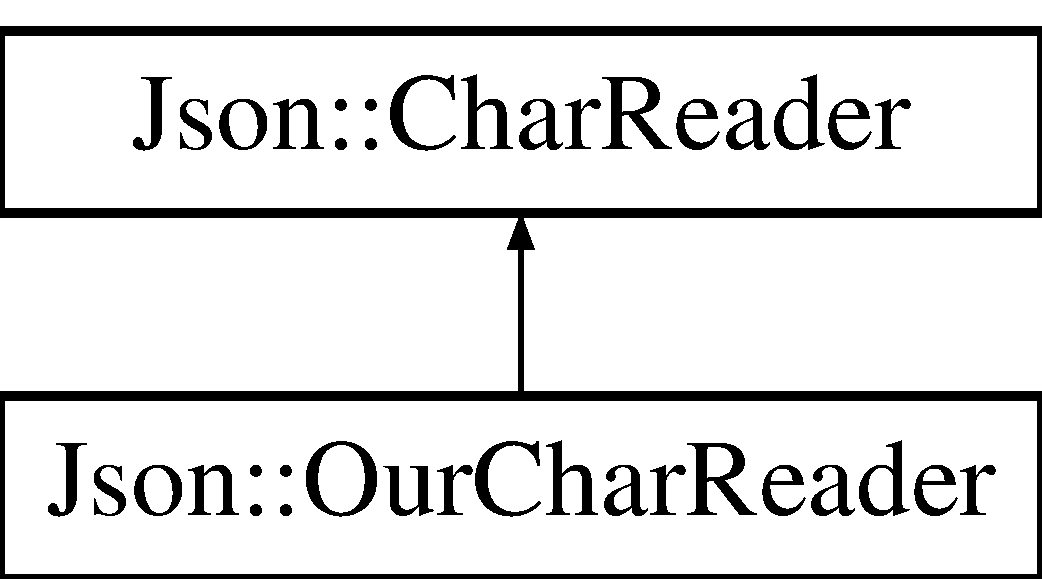
\includegraphics[height=2.000000cm]{classJson_1_1CharReader}
\end{center}
\end{figure}
\subsection*{Classes}
\begin{DoxyCompactItemize}
\item 
class \hyperlink{classJson_1_1CharReader_1_1Factory}{Factory}
\end{DoxyCompactItemize}
\subsection*{Public Member Functions}
\begin{DoxyCompactItemize}
\item 
virtual \hyperlink{classJson_1_1CharReader_acaa7b6ad04fe1cf2ddfca06e66550d7e}{$\sim$\+Char\+Reader} ()
\item 
virtual bool \hyperlink{classJson_1_1CharReader_a7983680d50fd0745f371c43b162e78e1}{parse} (char const $\ast$begin\+Doc, char const $\ast$end\+Doc, \hyperlink{classJson_1_1Value}{Value} $\ast$root, \hyperlink{json_8hpp_a1e723f95759de062585bc4a8fd3fa4be}{J\+S\+O\+N\+C\+P\+P\+\_\+\+S\+T\+R\+I\+NG} $\ast$errs)=0
\begin{DoxyCompactList}\small\item\em Read a \hyperlink{classJson_1_1Value}{Value} from a \href{http://www.json.org}{\tt J\+S\+ON} document. \end{DoxyCompactList}\end{DoxyCompactItemize}


\subsection{Detailed Description}
Interface for reading J\+S\+ON from a char array. 

\subsection{Constructor \& Destructor Documentation}
\index{Json\+::\+Char\+Reader@{Json\+::\+Char\+Reader}!````~Char\+Reader@{$\sim$\+Char\+Reader}}
\index{````~Char\+Reader@{$\sim$\+Char\+Reader}!Json\+::\+Char\+Reader@{Json\+::\+Char\+Reader}}
\subsubsection[{\texorpdfstring{$\sim$\+Char\+Reader()}{~CharReader()}}]{\setlength{\rightskip}{0pt plus 5cm}virtual Json\+::\+Char\+Reader\+::$\sim$\+Char\+Reader (
\begin{DoxyParamCaption}
{}
\end{DoxyParamCaption}
)\hspace{0.3cm}{\ttfamily [inline]}, {\ttfamily [virtual]}}\hypertarget{classJson_1_1CharReader_acaa7b6ad04fe1cf2ddfca06e66550d7e}{}\label{classJson_1_1CharReader_acaa7b6ad04fe1cf2ddfca06e66550d7e}


\subsection{Member Function Documentation}
\index{Json\+::\+Char\+Reader@{Json\+::\+Char\+Reader}!parse@{parse}}
\index{parse@{parse}!Json\+::\+Char\+Reader@{Json\+::\+Char\+Reader}}
\subsubsection[{\texorpdfstring{parse(char const $\ast$begin\+Doc, char const $\ast$end\+Doc, Value $\ast$root, J\+S\+O\+N\+C\+P\+P\+\_\+\+S\+T\+R\+I\+N\+G $\ast$errs)=0}{parse(char const *beginDoc, char const *endDoc, Value *root, JSONCPP_STRING *errs)=0}}]{\setlength{\rightskip}{0pt plus 5cm}virtual bool Json\+::\+Char\+Reader\+::parse (
\begin{DoxyParamCaption}
\item[{char const $\ast$}]{begin\+Doc, }
\item[{char const $\ast$}]{end\+Doc, }
\item[{{\bf Value} $\ast$}]{root, }
\item[{{\bf J\+S\+O\+N\+C\+P\+P\+\_\+\+S\+T\+R\+I\+NG} $\ast$}]{errs}
\end{DoxyParamCaption}
)\hspace{0.3cm}{\ttfamily [pure virtual]}}\hypertarget{classJson_1_1CharReader_a7983680d50fd0745f371c43b162e78e1}{}\label{classJson_1_1CharReader_a7983680d50fd0745f371c43b162e78e1}


Read a \hyperlink{classJson_1_1Value}{Value} from a \href{http://www.json.org}{\tt J\+S\+ON} document. 

The document must be a U\+T\+F-\/8 encoded string containing the document to read.


\begin{DoxyParams}{Parameters}
{\em begin\+Doc} & Pointer on the beginning of the U\+T\+F-\/8 encoded string of the document to read. \\
\hline
{\em end\+Doc} & Pointer on the end of the U\+T\+F-\/8 encoded string of the document to read. Must be $>$= begin\+Doc. \\
\hline
{\em root} & \mbox{[}out\mbox{]} Contains the root value of the document if it was successfully parsed. \\
\hline
{\em errs} & \mbox{[}out\mbox{]} Formatted error messages (if not N\+U\+LL) a user friendly string that lists errors in the parsed document. \\
\hline
\end{DoxyParams}
\begin{DoxyReturn}{Returns}
{\ttfamily true} if the document was successfully parsed, {\ttfamily false} if an error occurred. 
\end{DoxyReturn}


Implemented in \hyperlink{classJson_1_1OurCharReader_a547f08ec5a9951ca69e8bb2e90296c83}{Json\+::\+Our\+Char\+Reader}.



The documentation for this class was generated from the following file\+:\begin{DoxyCompactItemize}
\item 
/home/pranav/\+Repositories/zcm/include/\hyperlink{json_8hpp}{json.\+hpp}\end{DoxyCompactItemize}

\hypertarget{classJson_1_1CharReaderBuilder}{}\section{Json\+:\+:Char\+Reader\+Builder Class Reference}
\label{classJson_1_1CharReaderBuilder}\index{Json\+::\+Char\+Reader\+Builder@{Json\+::\+Char\+Reader\+Builder}}


Build a \hyperlink{classJson_1_1CharReader}{Char\+Reader} implementation.  




{\ttfamily \#include $<$json.\+hpp$>$}

Inheritance diagram for Json\+:\+:Char\+Reader\+Builder\+:\begin{figure}[H]
\begin{center}
\leavevmode
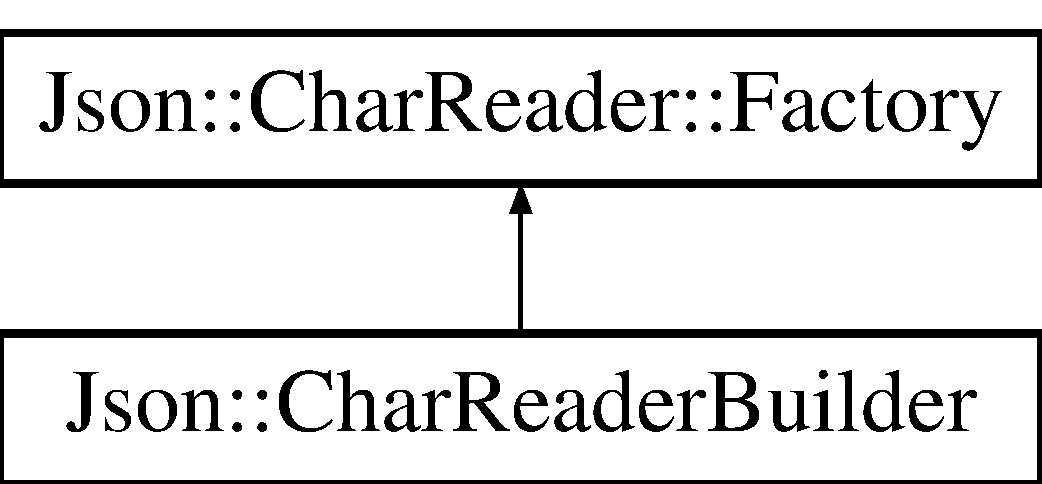
\includegraphics[height=2.000000cm]{classJson_1_1CharReaderBuilder}
\end{center}
\end{figure}
\subsection*{Public Member Functions}
\begin{DoxyCompactItemize}
\item 
\hyperlink{classJson_1_1CharReaderBuilder_a6e197b69a2ede3d87b03b9c5c78ba46a}{Char\+Reader\+Builder} ()
\item 
\hyperlink{classJson_1_1CharReaderBuilder_ae8226503f5b947e9d618c39dd992c85c}{$\sim$\+Char\+Reader\+Builder} () \hyperlink{json_8hpp_a824d6199c91488107e443226fa6022c5}{J\+S\+O\+N\+C\+P\+P\+\_\+\+O\+V\+E\+R\+R\+I\+DE}
\item 
\hyperlink{classJson_1_1CharReader}{Char\+Reader} $\ast$ \hyperlink{classJson_1_1CharReaderBuilder_a3a262fcc76c1eb8eebfd4718fb4e9722}{new\+Char\+Reader} () const \hyperlink{json_8hpp_a824d6199c91488107e443226fa6022c5}{J\+S\+O\+N\+C\+P\+P\+\_\+\+O\+V\+E\+R\+R\+I\+DE}
\begin{DoxyCompactList}\small\item\em Allocate a \hyperlink{classJson_1_1CharReader}{Char\+Reader} via operator new(). \end{DoxyCompactList}\item 
bool \hyperlink{classJson_1_1CharReaderBuilder_a3d233735a1e4b3c9a2cb9c68f972c02a}{validate} (\hyperlink{classJson_1_1Value}{Json\+::\+Value} $\ast$invalid) const 
\item 
\hyperlink{classJson_1_1Value}{Value} \& \hyperlink{classJson_1_1CharReaderBuilder_a84b35ef443340c06c0aa7b47851d8d86}{operator\mbox{[}$\,$\mbox{]}} (\hyperlink{json_8hpp_a1e723f95759de062585bc4a8fd3fa4be}{J\+S\+O\+N\+C\+P\+P\+\_\+\+S\+T\+R\+I\+NG} key)
\begin{DoxyCompactList}\small\item\em A simple way to update a specific setting. \end{DoxyCompactList}\end{DoxyCompactItemize}
\subsection*{Static Public Member Functions}
\begin{DoxyCompactItemize}
\item 
static void \hyperlink{classJson_1_1CharReaderBuilder_a03ff031e06aabff989ab4addc87294ab}{set\+Defaults} (\hyperlink{classJson_1_1Value}{Json\+::\+Value} $\ast$settings)
\begin{DoxyCompactList}\small\item\em Called by ctor, but you can use this to reset settings\+\_\+. \end{DoxyCompactList}\item 
static void \hyperlink{classJson_1_1CharReaderBuilder_a9c19e3c5475f9072d527810d4bf56749}{strict\+Mode} (\hyperlink{classJson_1_1Value}{Json\+::\+Value} $\ast$settings)
\begin{DoxyCompactList}\small\item\em Same as old \hyperlink{classJson_1_1Features_ae23176c14b2e79e81fb61fb1a8ab58ee}{Features\+::strict\+Mode()}. \end{DoxyCompactList}\end{DoxyCompactItemize}
\subsection*{Public Attributes}
\begin{DoxyCompactItemize}
\item 
\hyperlink{classJson_1_1Value}{Json\+::\+Value} \hyperlink{classJson_1_1CharReaderBuilder_ac69b7911ad64c171c51ebaf2ea26d958}{settings\+\_\+}
\begin{DoxyCompactList}\small\item\em Configuration of this builder. \end{DoxyCompactList}\end{DoxyCompactItemize}


\subsection{Detailed Description}
Build a \hyperlink{classJson_1_1CharReader}{Char\+Reader} implementation. 

Usage\+: 
\begin{DoxyCode}
\textcolor{keyword}{using namespace }\hyperlink{namespaceJson}{Json};
\hyperlink{classJson_1_1CharReaderBuilder}{CharReaderBuilder} builder;
builder[\textcolor{stringliteral}{"collectComments"}] = \textcolor{keyword}{false};
\hyperlink{classJson_1_1Value}{Value} value;
\hyperlink{json_8hpp_a1e723f95759de062585bc4a8fd3fa4be}{JSONCPP\_STRING} errs;
\textcolor{keywordtype}{bool} ok = \hyperlink{namespaceJson_a38f903cfdb57a6c4e86a7dcc42f3712c}{parseFromStream}(builder, std::cin, &value, &errs);
\end{DoxyCode}
 

\subsection{Constructor \& Destructor Documentation}
\index{Json\+::\+Char\+Reader\+Builder@{Json\+::\+Char\+Reader\+Builder}!Char\+Reader\+Builder@{Char\+Reader\+Builder}}
\index{Char\+Reader\+Builder@{Char\+Reader\+Builder}!Json\+::\+Char\+Reader\+Builder@{Json\+::\+Char\+Reader\+Builder}}
\subsubsection[{\texorpdfstring{Char\+Reader\+Builder()}{CharReaderBuilder()}}]{\setlength{\rightskip}{0pt plus 5cm}Json\+::\+Char\+Reader\+Builder\+::\+Char\+Reader\+Builder (
\begin{DoxyParamCaption}
{}
\end{DoxyParamCaption}
)}\hypertarget{classJson_1_1CharReaderBuilder_a6e197b69a2ede3d87b03b9c5c78ba46a}{}\label{classJson_1_1CharReaderBuilder_a6e197b69a2ede3d87b03b9c5c78ba46a}
\index{Json\+::\+Char\+Reader\+Builder@{Json\+::\+Char\+Reader\+Builder}!````~Char\+Reader\+Builder@{$\sim$\+Char\+Reader\+Builder}}
\index{````~Char\+Reader\+Builder@{$\sim$\+Char\+Reader\+Builder}!Json\+::\+Char\+Reader\+Builder@{Json\+::\+Char\+Reader\+Builder}}
\subsubsection[{\texorpdfstring{$\sim$\+Char\+Reader\+Builder() J\+S\+O\+N\+C\+P\+P\+\_\+\+O\+V\+E\+R\+R\+I\+DE}{~CharReaderBuilder() JSONCPP_OVERRIDE}}]{\setlength{\rightskip}{0pt plus 5cm}Json\+::\+Char\+Reader\+Builder\+::$\sim$\+Char\+Reader\+Builder (
\begin{DoxyParamCaption}
{}
\end{DoxyParamCaption}
)}\hypertarget{classJson_1_1CharReaderBuilder_ae8226503f5b947e9d618c39dd992c85c}{}\label{classJson_1_1CharReaderBuilder_ae8226503f5b947e9d618c39dd992c85c}


\subsection{Member Function Documentation}
\index{Json\+::\+Char\+Reader\+Builder@{Json\+::\+Char\+Reader\+Builder}!new\+Char\+Reader@{new\+Char\+Reader}}
\index{new\+Char\+Reader@{new\+Char\+Reader}!Json\+::\+Char\+Reader\+Builder@{Json\+::\+Char\+Reader\+Builder}}
\subsubsection[{\texorpdfstring{new\+Char\+Reader() const J\+S\+O\+N\+C\+P\+P\+\_\+\+O\+V\+E\+R\+R\+I\+DE}{newCharReader() const JSONCPP_OVERRIDE}}]{\setlength{\rightskip}{0pt plus 5cm}{\bf Char\+Reader} $\ast$ Json\+::\+Char\+Reader\+Builder\+::new\+Char\+Reader (
\begin{DoxyParamCaption}
{}
\end{DoxyParamCaption}
) const\hspace{0.3cm}{\ttfamily [virtual]}}\hypertarget{classJson_1_1CharReaderBuilder_a3a262fcc76c1eb8eebfd4718fb4e9722}{}\label{classJson_1_1CharReaderBuilder_a3a262fcc76c1eb8eebfd4718fb4e9722}


Allocate a \hyperlink{classJson_1_1CharReader}{Char\+Reader} via operator new(). 


\begin{DoxyExceptions}{Exceptions}
{\em std\+::exception} & if something goes wrong (e.\+g. invalid settings) \\
\hline
\end{DoxyExceptions}


Implements \hyperlink{classJson_1_1CharReader_1_1Factory_a4c5862a1ffd432372dbe65cf59de98c4}{Json\+::\+Char\+Reader\+::\+Factory}.

\index{Json\+::\+Char\+Reader\+Builder@{Json\+::\+Char\+Reader\+Builder}!operator\mbox{[}$\,$\mbox{]}@{operator[]}}
\index{operator\mbox{[}$\,$\mbox{]}@{operator[]}!Json\+::\+Char\+Reader\+Builder@{Json\+::\+Char\+Reader\+Builder}}
\subsubsection[{\texorpdfstring{operator[](\+J\+S\+O\+N\+C\+P\+P\+\_\+\+S\+T\+R\+I\+N\+G key)}{operator[](JSONCPP_STRING key)}}]{\setlength{\rightskip}{0pt plus 5cm}{\bf Value} \& Json\+::\+Char\+Reader\+Builder\+::operator\mbox{[}$\,$\mbox{]} (
\begin{DoxyParamCaption}
\item[{{\bf J\+S\+O\+N\+C\+P\+P\+\_\+\+S\+T\+R\+I\+NG}}]{key}
\end{DoxyParamCaption}
)}\hypertarget{classJson_1_1CharReaderBuilder_a84b35ef443340c06c0aa7b47851d8d86}{}\label{classJson_1_1CharReaderBuilder_a84b35ef443340c06c0aa7b47851d8d86}


A simple way to update a specific setting. 

\index{Json\+::\+Char\+Reader\+Builder@{Json\+::\+Char\+Reader\+Builder}!set\+Defaults@{set\+Defaults}}
\index{set\+Defaults@{set\+Defaults}!Json\+::\+Char\+Reader\+Builder@{Json\+::\+Char\+Reader\+Builder}}
\subsubsection[{\texorpdfstring{set\+Defaults(\+Json\+::\+Value $\ast$settings)}{setDefaults(Json::Value *settings)}}]{\setlength{\rightskip}{0pt plus 5cm}void Json\+::\+Char\+Reader\+Builder\+::set\+Defaults (
\begin{DoxyParamCaption}
\item[{{\bf Json\+::\+Value} $\ast$}]{settings}
\end{DoxyParamCaption}
)\hspace{0.3cm}{\ttfamily [static]}}\hypertarget{classJson_1_1CharReaderBuilder_a03ff031e06aabff989ab4addc87294ab}{}\label{classJson_1_1CharReaderBuilder_a03ff031e06aabff989ab4addc87294ab}


Called by ctor, but you can use this to reset settings\+\_\+. 

\begin{DoxyPrecond}{Precondition}
\textquotesingle{}settings\textquotesingle{} != N\+U\+LL (but Json\+::null is fine) 
\end{DoxyPrecond}
\begin{DoxyRemark}{Remarks}
Defaults\+: 
\begin{DoxyCodeInclude}
\end{DoxyCodeInclude}

\end{DoxyRemark}
\mbox{[}Char\+Reader\+Builder\+Defaults\mbox{]}

\mbox{[}Char\+Reader\+Builder\+Defaults\mbox{]} \index{Json\+::\+Char\+Reader\+Builder@{Json\+::\+Char\+Reader\+Builder}!strict\+Mode@{strict\+Mode}}
\index{strict\+Mode@{strict\+Mode}!Json\+::\+Char\+Reader\+Builder@{Json\+::\+Char\+Reader\+Builder}}
\subsubsection[{\texorpdfstring{strict\+Mode(\+Json\+::\+Value $\ast$settings)}{strictMode(Json::Value *settings)}}]{\setlength{\rightskip}{0pt plus 5cm}void Json\+::\+Char\+Reader\+Builder\+::strict\+Mode (
\begin{DoxyParamCaption}
\item[{{\bf Json\+::\+Value} $\ast$}]{settings}
\end{DoxyParamCaption}
)\hspace{0.3cm}{\ttfamily [static]}}\hypertarget{classJson_1_1CharReaderBuilder_a9c19e3c5475f9072d527810d4bf56749}{}\label{classJson_1_1CharReaderBuilder_a9c19e3c5475f9072d527810d4bf56749}


Same as old \hyperlink{classJson_1_1Features_ae23176c14b2e79e81fb61fb1a8ab58ee}{Features\+::strict\+Mode()}. 

\begin{DoxyPrecond}{Precondition}
\textquotesingle{}settings\textquotesingle{} != N\+U\+LL (but Json\+::null is fine) 
\end{DoxyPrecond}
\begin{DoxyRemark}{Remarks}
Defaults\+: 
\begin{DoxyCodeInclude}
\end{DoxyCodeInclude}

\end{DoxyRemark}
\mbox{[}Char\+Reader\+Builder\+Strict\+Mode\mbox{]}

\mbox{[}Char\+Reader\+Builder\+Strict\+Mode\mbox{]} \index{Json\+::\+Char\+Reader\+Builder@{Json\+::\+Char\+Reader\+Builder}!validate@{validate}}
\index{validate@{validate}!Json\+::\+Char\+Reader\+Builder@{Json\+::\+Char\+Reader\+Builder}}
\subsubsection[{\texorpdfstring{validate(\+Json\+::\+Value $\ast$invalid) const }{validate(Json::Value *invalid) const }}]{\setlength{\rightskip}{0pt plus 5cm}bool Json\+::\+Char\+Reader\+Builder\+::validate (
\begin{DoxyParamCaption}
\item[{{\bf Json\+::\+Value} $\ast$}]{invalid}
\end{DoxyParamCaption}
) const}\hypertarget{classJson_1_1CharReaderBuilder_a3d233735a1e4b3c9a2cb9c68f972c02a}{}\label{classJson_1_1CharReaderBuilder_a3d233735a1e4b3c9a2cb9c68f972c02a}
\begin{DoxyReturn}{Returns}
true if \textquotesingle{}settings\textquotesingle{} are legal and consistent; otherwise, indicate bad settings via \textquotesingle{}invalid\textquotesingle{}. 
\end{DoxyReturn}


\subsection{Member Data Documentation}
\index{Json\+::\+Char\+Reader\+Builder@{Json\+::\+Char\+Reader\+Builder}!settings\+\_\+@{settings\+\_\+}}
\index{settings\+\_\+@{settings\+\_\+}!Json\+::\+Char\+Reader\+Builder@{Json\+::\+Char\+Reader\+Builder}}
\subsubsection[{\texorpdfstring{settings\+\_\+}{settings_}}]{\setlength{\rightskip}{0pt plus 5cm}{\bf Json\+::\+Value} Json\+::\+Char\+Reader\+Builder\+::settings\+\_\+}\hypertarget{classJson_1_1CharReaderBuilder_ac69b7911ad64c171c51ebaf2ea26d958}{}\label{classJson_1_1CharReaderBuilder_ac69b7911ad64c171c51ebaf2ea26d958}


Configuration of this builder. 

These are case-\/sensitive. Available settings (case-\/sensitive)\+:
\begin{DoxyItemize}
\item {\ttfamily \char`\"{}collect\+Comments\char`\"{}\+: false or true}
\begin{DoxyItemize}
\item true to collect comment and allow writing them back during serialization, false to discard comments. This parameter is ignored if allow\+Comments is false.
\end{DoxyItemize}
\item {\ttfamily \char`\"{}allow\+Comments\char`\"{}\+: false or true}
\begin{DoxyItemize}
\item true if comments are allowed.
\end{DoxyItemize}
\item {\ttfamily \char`\"{}strict\+Root\char`\"{}\+: false or true}
\begin{DoxyItemize}
\item true if root must be either an array or an object value
\end{DoxyItemize}
\item {\ttfamily \char`\"{}allow\+Dropped\+Null\+Placeholders\char`\"{}\+: false or true}
\begin{DoxyItemize}
\item true if dropped null placeholders are allowed. (See \hyperlink{classJson_1_1StreamWriterBuilder}{Stream\+Writer\+Builder}.)
\end{DoxyItemize}
\item {\ttfamily \char`\"{}allow\+Numeric\+Keys\char`\"{}\+: false or true}
\begin{DoxyItemize}
\item true if numeric object keys are allowed.
\end{DoxyItemize}
\item {\ttfamily \char`\"{}allow\+Single\+Quotes\char`\"{}\+: false or true}
\begin{DoxyItemize}
\item true if \textquotesingle{}\textquotesingle{} are allowed for strings (both keys and values)
\end{DoxyItemize}
\item {\ttfamily \char`\"{}stack\+Limit\char`\"{}\+: integer}
\begin{DoxyItemize}
\item Exceeding stack\+Limit (recursive depth of {\ttfamily read\+Value()}) will cause an exception.
\item This is a security issue (seg-\/faults caused by deeply nested J\+S\+ON), so the default is low.
\end{DoxyItemize}
\item {\ttfamily \char`\"{}fail\+If\+Extra\char`\"{}\+: false or true}
\begin{DoxyItemize}
\item If true, {\ttfamily parse()} returns false when extra non-\/whitespace trails the J\+S\+ON value in the input string.
\end{DoxyItemize}
\item {\ttfamily \char`\"{}reject\+Dup\+Keys\char`\"{}\+: false or true}
\begin{DoxyItemize}
\item If true, {\ttfamily parse()} returns false when a key is duplicated within an object.
\end{DoxyItemize}
\item {\ttfamily \char`\"{}allow\+Special\+Floats\char`\"{}\+: false or true}
\begin{DoxyItemize}
\item If true, special float values (Na\+Ns and infinities) are allowed and their values are lossfree restorable.
\end{DoxyItemize}
\end{DoxyItemize}

You can examine \textquotesingle{}settings\+\_\+` yourself to see the defaults. You can also write and read them just like any J\+S\+ON \hyperlink{classJson_1_1Value}{Value}. \begin{DoxySeeAlso}{See also}
\hyperlink{classJson_1_1CharReaderBuilder_a03ff031e06aabff989ab4addc87294ab}{set\+Defaults()} 
\end{DoxySeeAlso}


The documentation for this class was generated from the following files\+:\begin{DoxyCompactItemize}
\item 
/home/pranav/\+Repositories/zcm/include/\hyperlink{json_8hpp}{json.\+hpp}\item 
/home/pranav/\+Repositories/zcm/src/\hyperlink{json_8cpp}{json.\+cpp}\end{DoxyCompactItemize}

\hypertarget{classzcm_1_1Client}{\section{zcm\-:\-:Client Class Reference}
\label{classzcm_1_1Client}\index{zcm\-::\-Client@{zcm\-::\-Client}}
}


\hyperlink{classzcm_1_1Client}{Client} class.  




{\ttfamily \#include $<$client.\-hpp$>$}

\subsection*{Public Member Functions}
\begin{DoxyCompactItemize}
\item 
\hyperlink{classzcm_1_1Client_aeea4b7db3574a527009edc3f41310bcc}{Client} (std\-::string \hyperlink{classzcm_1_1Client_ae972b951134774fd2246d802e2bc6fc0}{name}, zmq\-::context\-\_\-t $\ast$actor\-\_\-context, int timeout)
\begin{DoxyCompactList}\small\item\em Construct a client object. \end{DoxyCompactList}\item 
\hyperlink{classzcm_1_1Client_a6002478c33c7c876de6b1b001121ff87}{Client} (std\-::string \hyperlink{classzcm_1_1Client_ae972b951134774fd2246d802e2bc6fc0}{name}, zmq\-::context\-\_\-t $\ast$actor\-\_\-context, std\-::vector$<$ std\-::string $>$ \hyperlink{classzcm_1_1Client_a01cfee292bb3546a47ec70fff35ff1b6}{endpoints}, int timeout)
\begin{DoxyCompactList}\small\item\em Construct a client object with known endpoints. \end{DoxyCompactList}\item 
\hyperlink{classzcm_1_1Client_a927b35854850369d4d95b3101f3a9baa}{$\sim$\-Client} ()
\begin{DoxyCompactList}\small\item\em Close the client Z\-M\-Q socket and destroy the context. \end{DoxyCompactList}\item 
void \hyperlink{classzcm_1_1Client_aabf03e1bc961b1e525cff57986b1b5a8}{connect} (std\-::vector$<$ std\-::string $>$ new\-\_\-endpoints)
\begin{DoxyCompactList}\small\item\em Connect the client to a new set of endpoints. \end{DoxyCompactList}\item 
std\-::string \hyperlink{classzcm_1_1Client_ad4178e9b209db19994204b9dad7aa374}{get\-\_\-name} ()
\begin{DoxyCompactList}\small\item\em Return the client name. \end{DoxyCompactList}\item 
void \hyperlink{classzcm_1_1Client_aec14e7e61a88c918df8c2bae729923b2}{set\-\_\-timeout} (int timeout)
\begin{DoxyCompactList}\small\item\em Set timeout on the client to prevent endless blocking. \end{DoxyCompactList}\item 
std\-::string \hyperlink{classzcm_1_1Client_a9f62555765181c2feee4631a4b50786d}{call} (std\-::string message)
\begin{DoxyCompactList}\small\item\em Call the server. \end{DoxyCompactList}\end{DoxyCompactItemize}
\subsection*{Private Attributes}
\begin{DoxyCompactItemize}
\item 
std\-::string \hyperlink{classzcm_1_1Client_ae972b951134774fd2246d802e2bc6fc0}{name}
\begin{DoxyCompactList}\small\item\em Name of the publisher. \end{DoxyCompactList}\item 
std\-::vector$<$ std\-::string $>$ \hyperlink{classzcm_1_1Client_a01cfee292bb3546a47ec70fff35ff1b6}{endpoints}
\begin{DoxyCompactList}\small\item\em Vector of endpoints to connect to. \end{DoxyCompactList}\item 
zmq\-::context\-\_\-t $\ast$ \hyperlink{classzcm_1_1Client_a0519b850f2a5167a0636f7a7adcabe1e}{context}
\begin{DoxyCompactList}\small\item\em Z\-M\-Q Context of the client. \end{DoxyCompactList}\item 
zmq\-::socket\-\_\-t $\ast$ \hyperlink{classzcm_1_1Client_a022f5e131d58cea7f6cc49b4580940a0}{client\-\_\-socket}
\begin{DoxyCompactList}\small\item\em Z\-M\-Q Socket of the client. \end{DoxyCompactList}\item 
int \hyperlink{classzcm_1_1Client_a25fa4ff78b8e962ca8436a8815bf7924}{client\-\_\-socket\-\_\-timeout}
\begin{DoxyCompactList}\small\item\em Timeout of the client socket. \end{DoxyCompactList}\end{DoxyCompactItemize}


\subsection{Detailed Description}
\hyperlink{classzcm_1_1Client}{Client} class. 

\subsection{Constructor \& Destructor Documentation}
\hypertarget{classzcm_1_1Client_aeea4b7db3574a527009edc3f41310bcc}{\index{zcm\-::\-Client@{zcm\-::\-Client}!Client@{Client}}
\index{Client@{Client}!zcm::Client@{zcm\-::\-Client}}
\subsubsection[{Client}]{\setlength{\rightskip}{0pt plus 5cm}zcm\-::\-Client\-::\-Client (
\begin{DoxyParamCaption}
\item[{std\-::string}]{name, }
\item[{zmq\-::context\-\_\-t $\ast$}]{actor\-\_\-context, }
\item[{int}]{timeout = {\ttfamily 500}}
\end{DoxyParamCaption}
)}}\label{classzcm_1_1Client_aeea4b7db3574a527009edc3f41310bcc}


Construct a client object. 


\begin{DoxyParams}[1]{Parameters}
\mbox{\tt in}  & {\em name} & \hyperlink{classzcm_1_1Client}{Client} name \\
\hline
\mbox{\tt in}  & {\em Z\-M\-Q} & Context of the \hyperlink{classzcm_1_1Actor}{Actor} Process \\
\hline
\mbox{\tt in}  & {\em timeout} & \hyperlink{classzcm_1_1Client}{Client} socket timeout \\
\hline
\end{DoxyParams}
\hypertarget{classzcm_1_1Client_a6002478c33c7c876de6b1b001121ff87}{\index{zcm\-::\-Client@{zcm\-::\-Client}!Client@{Client}}
\index{Client@{Client}!zcm::Client@{zcm\-::\-Client}}
\subsubsection[{Client}]{\setlength{\rightskip}{0pt plus 5cm}zcm\-::\-Client\-::\-Client (
\begin{DoxyParamCaption}
\item[{std\-::string}]{name, }
\item[{zmq\-::context\-\_\-t $\ast$}]{actor\-\_\-context, }
\item[{std\-::vector$<$ std\-::string $>$}]{endpoints, }
\item[{int}]{timeout = {\ttfamily 500}}
\end{DoxyParamCaption}
)}}\label{classzcm_1_1Client_a6002478c33c7c876de6b1b001121ff87}


Construct a client object with known endpoints. 


\begin{DoxyParams}[1]{Parameters}
\mbox{\tt in}  & {\em name} & \hyperlink{classzcm_1_1Client}{Client} name \\
\hline
\mbox{\tt in}  & {\em Z\-M\-Q} & Context of the \hyperlink{classzcm_1_1Actor}{Actor} Process \\
\hline
\mbox{\tt in}  & {\em endpoints} & A vector of endpoint strings \\
\hline
\mbox{\tt in}  & {\em timeout} & \hyperlink{classzcm_1_1Client}{Client} socket timeout \\
\hline
\end{DoxyParams}
\hypertarget{classzcm_1_1Client_a927b35854850369d4d95b3101f3a9baa}{\index{zcm\-::\-Client@{zcm\-::\-Client}!$\sim$\-Client@{$\sim$\-Client}}
\index{$\sim$\-Client@{$\sim$\-Client}!zcm::Client@{zcm\-::\-Client}}
\subsubsection[{$\sim$\-Client}]{\setlength{\rightskip}{0pt plus 5cm}zcm\-::\-Client\-::$\sim$\-Client (
\begin{DoxyParamCaption}
{}
\end{DoxyParamCaption}
)}}\label{classzcm_1_1Client_a927b35854850369d4d95b3101f3a9baa}


Close the client Z\-M\-Q socket and destroy the context. 



\subsection{Member Function Documentation}
\hypertarget{classzcm_1_1Client_a9f62555765181c2feee4631a4b50786d}{\index{zcm\-::\-Client@{zcm\-::\-Client}!call@{call}}
\index{call@{call}!zcm::Client@{zcm\-::\-Client}}
\subsubsection[{call}]{\setlength{\rightskip}{0pt plus 5cm}std\-::string zcm\-::\-Client\-::call (
\begin{DoxyParamCaption}
\item[{std\-::string}]{message}
\end{DoxyParamCaption}
)}}\label{classzcm_1_1Client_a9f62555765181c2feee4631a4b50786d}


Call the server. 


\begin{DoxyParams}[1]{Parameters}
\mbox{\tt in}  & {\em message} & The message string. Serialize complex objects to strings with protobuf \\
\hline
\end{DoxyParams}
\hypertarget{classzcm_1_1Client_aabf03e1bc961b1e525cff57986b1b5a8}{\index{zcm\-::\-Client@{zcm\-::\-Client}!connect@{connect}}
\index{connect@{connect}!zcm::Client@{zcm\-::\-Client}}
\subsubsection[{connect}]{\setlength{\rightskip}{0pt plus 5cm}void zcm\-::\-Client\-::connect (
\begin{DoxyParamCaption}
\item[{std\-::vector$<$ std\-::string $>$}]{new\-\_\-endpoints}
\end{DoxyParamCaption}
)}}\label{classzcm_1_1Client_aabf03e1bc961b1e525cff57986b1b5a8}


Connect the client to a new set of endpoints. 


\begin{DoxyParams}[1]{Parameters}
\mbox{\tt in}  & {\em new\-\_\-endpoints} & New set of endpoints as a vector \\
\hline
\end{DoxyParams}
\hypertarget{classzcm_1_1Client_ad4178e9b209db19994204b9dad7aa374}{\index{zcm\-::\-Client@{zcm\-::\-Client}!get\-\_\-name@{get\-\_\-name}}
\index{get\-\_\-name@{get\-\_\-name}!zcm::Client@{zcm\-::\-Client}}
\subsubsection[{get\-\_\-name}]{\setlength{\rightskip}{0pt plus 5cm}std\-::string zcm\-::\-Client\-::get\-\_\-name (
\begin{DoxyParamCaption}
{}
\end{DoxyParamCaption}
)}}\label{classzcm_1_1Client_ad4178e9b209db19994204b9dad7aa374}


Return the client name. 

\begin{DoxyReturn}{Returns}
\hyperlink{classzcm_1_1Client}{Client} name 
\end{DoxyReturn}
\hypertarget{classzcm_1_1Client_aec14e7e61a88c918df8c2bae729923b2}{\index{zcm\-::\-Client@{zcm\-::\-Client}!set\-\_\-timeout@{set\-\_\-timeout}}
\index{set\-\_\-timeout@{set\-\_\-timeout}!zcm::Client@{zcm\-::\-Client}}
\subsubsection[{set\-\_\-timeout}]{\setlength{\rightskip}{0pt plus 5cm}void zcm\-::\-Client\-::set\-\_\-timeout (
\begin{DoxyParamCaption}
\item[{int}]{timeout}
\end{DoxyParamCaption}
)}}\label{classzcm_1_1Client_aec14e7e61a88c918df8c2bae729923b2}


Set timeout on the client to prevent endless blocking. 


\begin{DoxyParams}[1]{Parameters}
\mbox{\tt in}  & {\em timeout} & New timeout value \\
\hline
\end{DoxyParams}


\subsection{Member Data Documentation}
\hypertarget{classzcm_1_1Client_a022f5e131d58cea7f6cc49b4580940a0}{\index{zcm\-::\-Client@{zcm\-::\-Client}!client\-\_\-socket@{client\-\_\-socket}}
\index{client\-\_\-socket@{client\-\_\-socket}!zcm::Client@{zcm\-::\-Client}}
\subsubsection[{client\-\_\-socket}]{\setlength{\rightskip}{0pt plus 5cm}zmq\-::socket\-\_\-t$\ast$ zcm\-::\-Client\-::client\-\_\-socket\hspace{0.3cm}{\ttfamily [private]}}}\label{classzcm_1_1Client_a022f5e131d58cea7f6cc49b4580940a0}


Z\-M\-Q Socket of the client. 

\hypertarget{classzcm_1_1Client_a25fa4ff78b8e962ca8436a8815bf7924}{\index{zcm\-::\-Client@{zcm\-::\-Client}!client\-\_\-socket\-\_\-timeout@{client\-\_\-socket\-\_\-timeout}}
\index{client\-\_\-socket\-\_\-timeout@{client\-\_\-socket\-\_\-timeout}!zcm::Client@{zcm\-::\-Client}}
\subsubsection[{client\-\_\-socket\-\_\-timeout}]{\setlength{\rightskip}{0pt plus 5cm}int zcm\-::\-Client\-::client\-\_\-socket\-\_\-timeout\hspace{0.3cm}{\ttfamily [private]}}}\label{classzcm_1_1Client_a25fa4ff78b8e962ca8436a8815bf7924}


Timeout of the client socket. 

\hypertarget{classzcm_1_1Client_a0519b850f2a5167a0636f7a7adcabe1e}{\index{zcm\-::\-Client@{zcm\-::\-Client}!context@{context}}
\index{context@{context}!zcm::Client@{zcm\-::\-Client}}
\subsubsection[{context}]{\setlength{\rightskip}{0pt plus 5cm}zmq\-::context\-\_\-t$\ast$ zcm\-::\-Client\-::context\hspace{0.3cm}{\ttfamily [private]}}}\label{classzcm_1_1Client_a0519b850f2a5167a0636f7a7adcabe1e}


Z\-M\-Q Context of the client. 

\hypertarget{classzcm_1_1Client_a01cfee292bb3546a47ec70fff35ff1b6}{\index{zcm\-::\-Client@{zcm\-::\-Client}!endpoints@{endpoints}}
\index{endpoints@{endpoints}!zcm::Client@{zcm\-::\-Client}}
\subsubsection[{endpoints}]{\setlength{\rightskip}{0pt plus 5cm}std\-::vector$<$std\-::string$>$ zcm\-::\-Client\-::endpoints\hspace{0.3cm}{\ttfamily [private]}}}\label{classzcm_1_1Client_a01cfee292bb3546a47ec70fff35ff1b6}


Vector of endpoints to connect to. 

\hypertarget{classzcm_1_1Client_ae972b951134774fd2246d802e2bc6fc0}{\index{zcm\-::\-Client@{zcm\-::\-Client}!name@{name}}
\index{name@{name}!zcm::Client@{zcm\-::\-Client}}
\subsubsection[{name}]{\setlength{\rightskip}{0pt plus 5cm}std\-::string zcm\-::\-Client\-::name\hspace{0.3cm}{\ttfamily [private]}}}\label{classzcm_1_1Client_ae972b951134774fd2246d802e2bc6fc0}


Name of the publisher. 



The documentation for this class was generated from the following files\-:\begin{DoxyCompactItemize}
\item 
/home/kelsier/\-Git\-Hub/zcm/include/\hyperlink{client_8hpp}{client.\-hpp}\item 
/home/kelsier/\-Git\-Hub/zcm/src/\hyperlink{client_8cpp}{client.\-cpp}\end{DoxyCompactItemize}

\hypertarget{structJson_1_1Value_1_1CommentInfo}{}\section{Json\+:\+:Value\+:\+:Comment\+Info Struct Reference}
\label{structJson_1_1Value_1_1CommentInfo}\index{Json\+::\+Value\+::\+Comment\+Info@{Json\+::\+Value\+::\+Comment\+Info}}
\subsection*{Public Member Functions}
\begin{DoxyCompactItemize}
\item 
\hyperlink{structJson_1_1Value_1_1CommentInfo_ab23b0c125695d284bded2fb106a49043}{Comment\+Info} ()
\item 
\hyperlink{structJson_1_1Value_1_1CommentInfo_ab4d0877190bdbf484e4e2a3bade42ac8}{$\sim$\+Comment\+Info} ()
\item 
void \hyperlink{structJson_1_1Value_1_1CommentInfo_a4d01c2cd8c07995969c5d636dfd4fa8c}{set\+Comment} (const char $\ast$text, size\+\_\+t len)
\end{DoxyCompactItemize}
\subsection*{Public Attributes}
\begin{DoxyCompactItemize}
\item 
char $\ast$ \hyperlink{structJson_1_1Value_1_1CommentInfo_a020f19c7098bab8ec8fec14cd1a5afb9}{comment\+\_\+}
\end{DoxyCompactItemize}


\subsection{Constructor \& Destructor Documentation}
\index{Json\+::\+Value\+::\+Comment\+Info@{Json\+::\+Value\+::\+Comment\+Info}!Comment\+Info@{Comment\+Info}}
\index{Comment\+Info@{Comment\+Info}!Json\+::\+Value\+::\+Comment\+Info@{Json\+::\+Value\+::\+Comment\+Info}}
\subsubsection[{\texorpdfstring{Comment\+Info()}{CommentInfo()}}]{\setlength{\rightskip}{0pt plus 5cm}Json\+::\+Value\+::\+Comment\+Info\+::\+Comment\+Info (
\begin{DoxyParamCaption}
{}
\end{DoxyParamCaption}
)}\hypertarget{structJson_1_1Value_1_1CommentInfo_ab23b0c125695d284bded2fb106a49043}{}\label{structJson_1_1Value_1_1CommentInfo_ab23b0c125695d284bded2fb106a49043}
\index{Json\+::\+Value\+::\+Comment\+Info@{Json\+::\+Value\+::\+Comment\+Info}!````~Comment\+Info@{$\sim$\+Comment\+Info}}
\index{````~Comment\+Info@{$\sim$\+Comment\+Info}!Json\+::\+Value\+::\+Comment\+Info@{Json\+::\+Value\+::\+Comment\+Info}}
\subsubsection[{\texorpdfstring{$\sim$\+Comment\+Info()}{~CommentInfo()}}]{\setlength{\rightskip}{0pt plus 5cm}Json\+::\+Value\+::\+Comment\+Info\+::$\sim$\+Comment\+Info (
\begin{DoxyParamCaption}
{}
\end{DoxyParamCaption}
)}\hypertarget{structJson_1_1Value_1_1CommentInfo_ab4d0877190bdbf484e4e2a3bade42ac8}{}\label{structJson_1_1Value_1_1CommentInfo_ab4d0877190bdbf484e4e2a3bade42ac8}


\subsection{Member Function Documentation}
\index{Json\+::\+Value\+::\+Comment\+Info@{Json\+::\+Value\+::\+Comment\+Info}!set\+Comment@{set\+Comment}}
\index{set\+Comment@{set\+Comment}!Json\+::\+Value\+::\+Comment\+Info@{Json\+::\+Value\+::\+Comment\+Info}}
\subsubsection[{\texorpdfstring{set\+Comment(const char $\ast$text, size\+\_\+t len)}{setComment(const char *text, size_t len)}}]{\setlength{\rightskip}{0pt plus 5cm}void Json\+::\+Value\+::\+Comment\+Info\+::set\+Comment (
\begin{DoxyParamCaption}
\item[{const char $\ast$}]{text, }
\item[{size\+\_\+t}]{len}
\end{DoxyParamCaption}
)}\hypertarget{structJson_1_1Value_1_1CommentInfo_a4d01c2cd8c07995969c5d636dfd4fa8c}{}\label{structJson_1_1Value_1_1CommentInfo_a4d01c2cd8c07995969c5d636dfd4fa8c}


\subsection{Member Data Documentation}
\index{Json\+::\+Value\+::\+Comment\+Info@{Json\+::\+Value\+::\+Comment\+Info}!comment\+\_\+@{comment\+\_\+}}
\index{comment\+\_\+@{comment\+\_\+}!Json\+::\+Value\+::\+Comment\+Info@{Json\+::\+Value\+::\+Comment\+Info}}
\subsubsection[{\texorpdfstring{comment\+\_\+}{comment_}}]{\setlength{\rightskip}{0pt plus 5cm}char$\ast$ Json\+::\+Value\+::\+Comment\+Info\+::comment\+\_\+}\hypertarget{structJson_1_1Value_1_1CommentInfo_a020f19c7098bab8ec8fec14cd1a5afb9}{}\label{structJson_1_1Value_1_1CommentInfo_a020f19c7098bab8ec8fec14cd1a5afb9}


The documentation for this struct was generated from the following files\+:\begin{DoxyCompactItemize}
\item 
/home/pranav/\+Repositories/zcm/include/\hyperlink{json_8hpp}{json.\+hpp}\item 
/home/pranav/\+Repositories/zcm/src/\hyperlink{json_8cpp}{json.\+cpp}\end{DoxyCompactItemize}

\hypertarget{structJson_1_1CommentStyle}{}\section{Json\+:\+:Comment\+Style Struct Reference}
\label{structJson_1_1CommentStyle}\index{Json\+::\+Comment\+Style@{Json\+::\+Comment\+Style}}


Scoped enums are not available until C++11.  


\subsection*{Public Types}
\begin{DoxyCompactItemize}
\item 
enum \hyperlink{structJson_1_1CommentStyle_a51fc08f3518fd81eba12f340d19a3d0c}{Enum} \{ \hyperlink{structJson_1_1CommentStyle_a51fc08f3518fd81eba12f340d19a3d0cac8b32a8bae63414c8647d4919da8d437}{None}, 
\hyperlink{structJson_1_1CommentStyle_a51fc08f3518fd81eba12f340d19a3d0cac65238f050773c107690a456e9c05c98}{Most}, 
\hyperlink{structJson_1_1CommentStyle_a51fc08f3518fd81eba12f340d19a3d0ca32302c0b97190c1808b3e38f367fef01}{All}
 \}\begin{DoxyCompactList}\small\item\em Decide whether to write comments. \end{DoxyCompactList}
\end{DoxyCompactItemize}


\subsection{Detailed Description}
Scoped enums are not available until C++11. 

\subsection{Member Enumeration Documentation}
\index{Json\+::\+Comment\+Style@{Json\+::\+Comment\+Style}!Enum@{Enum}}
\index{Enum@{Enum}!Json\+::\+Comment\+Style@{Json\+::\+Comment\+Style}}
\subsubsection[{\texorpdfstring{Enum}{Enum}}]{\setlength{\rightskip}{0pt plus 5cm}enum {\bf Json\+::\+Comment\+Style\+::\+Enum}}\hypertarget{structJson_1_1CommentStyle_a51fc08f3518fd81eba12f340d19a3d0c}{}\label{structJson_1_1CommentStyle_a51fc08f3518fd81eba12f340d19a3d0c}


Decide whether to write comments. 

\begin{Desc}
\item[Enumerator]\par
\begin{description}
\index{None@{None}!Json\+::\+Comment\+Style@{Json\+::\+Comment\+Style}}\index{Json\+::\+Comment\+Style@{Json\+::\+Comment\+Style}!None@{None}}\item[{\em 
None\hypertarget{structJson_1_1CommentStyle_a51fc08f3518fd81eba12f340d19a3d0cac8b32a8bae63414c8647d4919da8d437}{}\label{structJson_1_1CommentStyle_a51fc08f3518fd81eba12f340d19a3d0cac8b32a8bae63414c8647d4919da8d437}
}]Drop all comments. \index{Most@{Most}!Json\+::\+Comment\+Style@{Json\+::\+Comment\+Style}}\index{Json\+::\+Comment\+Style@{Json\+::\+Comment\+Style}!Most@{Most}}\item[{\em 
Most\hypertarget{structJson_1_1CommentStyle_a51fc08f3518fd81eba12f340d19a3d0cac65238f050773c107690a456e9c05c98}{}\label{structJson_1_1CommentStyle_a51fc08f3518fd81eba12f340d19a3d0cac65238f050773c107690a456e9c05c98}
}]Recover odd behavior of previous versions (not implemented yet). \index{All@{All}!Json\+::\+Comment\+Style@{Json\+::\+Comment\+Style}}\index{Json\+::\+Comment\+Style@{Json\+::\+Comment\+Style}!All@{All}}\item[{\em 
All\hypertarget{structJson_1_1CommentStyle_a51fc08f3518fd81eba12f340d19a3d0ca32302c0b97190c1808b3e38f367fef01}{}\label{structJson_1_1CommentStyle_a51fc08f3518fd81eba12f340d19a3d0ca32302c0b97190c1808b3e38f367fef01}
}]Keep all comments. \end{description}
\end{Desc}


The documentation for this struct was generated from the following file\+:\begin{DoxyCompactItemize}
\item 
/home/pranav/\+Repositories/zcm/src/\hyperlink{json_8cpp}{json.\+cpp}\end{DoxyCompactItemize}

\hypertarget{classzcm_1_1Component}{}\section{zcm\+:\+:Component Class Reference}
\label{classzcm_1_1Component}\index{zcm\+::\+Component@{zcm\+::\+Component}}


\hyperlink{classzcm_1_1Component}{Component} class.  




{\ttfamily \#include $<$component.\+hpp$>$}

\subsection*{Public Member Functions}
\begin{DoxyCompactItemize}
\item 
\hyperlink{classzcm_1_1Component_a6fd6b1f309a6b464a14c22a94d18f040}{Component} ()
\begin{DoxyCompactList}\small\item\em Construct a component Prepare the component operation queue. \end{DoxyCompactList}\item 
\hyperlink{classzcm_1_1Component_a0bab6bb89e49affa281179f5d6aeff6a}{$\sim$\+Component} ()
\begin{DoxyCompactList}\small\item\em Destroy the component. \end{DoxyCompactList}\item 
\hyperlink{classzcm_1_1Timer}{Timer} $\ast$ \hyperlink{classzcm_1_1Component_a9fe1a846945403f152e069917f2f49b2}{get\+\_\+timer} (std\+::string timer\+\_\+name)
\begin{DoxyCompactList}\small\item\em Get a component timer by name. \end{DoxyCompactList}\item 
\hyperlink{classzcm_1_1Publisher}{Publisher} $\ast$ \hyperlink{classzcm_1_1Component_a9bbbc50ea3f1a278bf74848f784df493}{get\+\_\+publisher} (std\+::string publisher\+\_\+name)
\begin{DoxyCompactList}\small\item\em Get a component publisher by name. \end{DoxyCompactList}\item 
\hyperlink{classzcm_1_1Subscriber}{Subscriber} $\ast$ \hyperlink{classzcm_1_1Component_a4865551765c7d0ead713ad65571aa8dc}{get\+\_\+subscriber} (std\+::string subscriber\+\_\+name)
\begin{DoxyCompactList}\small\item\em Get a component subscriber by name. \end{DoxyCompactList}\item 
\hyperlink{classzcm_1_1Client}{Client} $\ast$ \hyperlink{classzcm_1_1Component_a89e3f610505b007767f10235b4ea8c20}{get\+\_\+client} (std\+::string client\+\_\+name)
\begin{DoxyCompactList}\small\item\em Get a component client by name. \end{DoxyCompactList}\item 
\hyperlink{classzcm_1_1Server}{Server} $\ast$ \hyperlink{classzcm_1_1Component_a80e221012442119feb53740510242117}{get\+\_\+server} (std\+::string server\+\_\+name)
\begin{DoxyCompactList}\small\item\em Get a component server by name. \end{DoxyCompactList}\item 
void \hyperlink{classzcm_1_1Component_ac9b656236674930c58f7dbfebb063da9}{add\+\_\+timer} (\hyperlink{classzcm_1_1Timer}{Timer} $\ast$new\+\_\+timer)
\begin{DoxyCompactList}\small\item\em Add a timer to this component. \end{DoxyCompactList}\item 
void \hyperlink{classzcm_1_1Component_a3d70420843fc7e0ff2d3d2edc422e992}{add\+\_\+publisher} (\hyperlink{classzcm_1_1Publisher}{Publisher} $\ast$new\+\_\+publisher)
\begin{DoxyCompactList}\small\item\em Add a publisher to this component. \end{DoxyCompactList}\item 
void \hyperlink{classzcm_1_1Component_ac07614093c36e61704d166f00f14c22e}{add\+\_\+subscriber} (\hyperlink{classzcm_1_1Subscriber}{Subscriber} $\ast$new\+\_\+subscriber)
\begin{DoxyCompactList}\small\item\em Add a subscriber to this component. \end{DoxyCompactList}\item 
void \hyperlink{classzcm_1_1Component_ad71bf4cebc218089642d16f697a493fa}{add\+\_\+client} (\hyperlink{classzcm_1_1Client}{Client} $\ast$new\+\_\+client)
\begin{DoxyCompactList}\small\item\em Add a client to this component. \end{DoxyCompactList}\item 
void \hyperlink{classzcm_1_1Component_a31989e75d9de6093cb712148cd94da71}{add\+\_\+server} (\hyperlink{classzcm_1_1Server}{Server} $\ast$new\+\_\+server)
\begin{DoxyCompactList}\small\item\em Add a server to this component. \end{DoxyCompactList}\item 
void \hyperlink{classzcm_1_1Component_a64674700fb1edd7c84a64ce78aa5b2f4}{configure\+\_\+publishers} (std\+::map$<$ std\+::string, std\+::vector$<$ std\+::string $>$$>$ publisher\+\_\+endpoints)
\begin{DoxyCompactList}\small\item\em Configure all component publishers. \end{DoxyCompactList}\item 
void \hyperlink{classzcm_1_1Component_a25c31193982bb317186f4f3b4d8d790c}{configure\+\_\+subscribers} (std\+::map$<$ std\+::string, std\+::vector$<$ std\+::string $>$$>$ subscriber\+\_\+endpoints)
\begin{DoxyCompactList}\small\item\em Configure all component subscribers. \end{DoxyCompactList}\item 
void \hyperlink{classzcm_1_1Component_ad3ed49fb7e936de3fd66ac4e37974735}{configure\+\_\+clients} (std\+::map$<$ std\+::string, std\+::vector$<$ std\+::string $>$$>$ client\+\_\+endpoints)
\begin{DoxyCompactList}\small\item\em Configure all component clients. \end{DoxyCompactList}\item 
void \hyperlink{classzcm_1_1Component_a9a8df5c1a899ec4470dd5bbcd90e9e79}{configure\+\_\+servers} (std\+::map$<$ std\+::string, std\+::vector$<$ std\+::string $>$$>$ server\+\_\+endpoints)
\begin{DoxyCompactList}\small\item\em Configure all component servers. \end{DoxyCompactList}\item 
std\+::thread $\ast$ \hyperlink{classzcm_1_1Component_a328d6f79aab5455e96a2badfdb6bb451}{spawn} ()
\begin{DoxyCompactList}\small\item\em Spawn the component executor thread. \end{DoxyCompactList}\end{DoxyCompactItemize}
\subsection*{Protected Attributes}
\begin{DoxyCompactItemize}
\item 
\hyperlink{classzcm_1_1Operation__Queue}{Operation\+\_\+\+Queue} $\ast$ \hyperlink{classzcm_1_1Component_a4c9f3591c18dde89bc3c2af7717c6692}{operation\+\_\+queue}
\begin{DoxyCompactList}\small\item\em Pointer to the \hyperlink{classzcm_1_1Component}{Component} Operation Queue. \end{DoxyCompactList}\item 
std\+::thread $\ast$ \hyperlink{classzcm_1_1Component_a392ca3b6cd537cd7aa1d4db31dacdf4d}{executor\+\_\+thread}
\begin{DoxyCompactList}\small\item\em Pointer to the \hyperlink{classzcm_1_1Component}{Component} Executor Thread. \end{DoxyCompactList}\item 
std\+::vector$<$ \hyperlink{classzcm_1_1Timer}{Timer} $\ast$ $>$ \hyperlink{classzcm_1_1Component_a506eac4aebc9e02f0df246afbbac7d75}{timers}
\begin{DoxyCompactList}\small\item\em A vector of component timers. \end{DoxyCompactList}\item 
std\+::vector$<$ \hyperlink{classzcm_1_1Publisher}{Publisher} $\ast$ $>$ \hyperlink{classzcm_1_1Component_a4dcce63b0b5495bc15bd18e5dce86094}{publishers}
\begin{DoxyCompactList}\small\item\em A vector of component publishers. \end{DoxyCompactList}\item 
std\+::vector$<$ \hyperlink{classzcm_1_1Subscriber}{Subscriber} $\ast$ $>$ \hyperlink{classzcm_1_1Component_a9f9e58fb5d2189b183ffd22ce905d620}{subscribers}
\begin{DoxyCompactList}\small\item\em A vector of component subscribers. \end{DoxyCompactList}\item 
std\+::vector$<$ \hyperlink{classzcm_1_1Client}{Client} $\ast$ $>$ \hyperlink{classzcm_1_1Component_a940e1b9755cd9f2bea95bda880999626}{clients}
\begin{DoxyCompactList}\small\item\em A vector of component clients. \end{DoxyCompactList}\item 
std\+::vector$<$ \hyperlink{classzcm_1_1Server}{Server} $\ast$ $>$ \hyperlink{classzcm_1_1Component_a1d99508f165f7014b190d2fbe4ad2271}{servers}
\begin{DoxyCompactList}\small\item\em A vector of component servers. \end{DoxyCompactList}\end{DoxyCompactItemize}


\subsection{Detailed Description}
\hyperlink{classzcm_1_1Component}{Component} class. 

\subsection{Constructor \& Destructor Documentation}
\index{zcm\+::\+Component@{zcm\+::\+Component}!Component@{Component}}
\index{Component@{Component}!zcm\+::\+Component@{zcm\+::\+Component}}
\subsubsection[{\texorpdfstring{Component()}{Component()}}]{\setlength{\rightskip}{0pt plus 5cm}zcm\+::\+Component\+::\+Component (
\begin{DoxyParamCaption}
{}
\end{DoxyParamCaption}
)}\hypertarget{classzcm_1_1Component_a6fd6b1f309a6b464a14c22a94d18f040}{}\label{classzcm_1_1Component_a6fd6b1f309a6b464a14c22a94d18f040}


Construct a component Prepare the component operation queue. 

\index{zcm\+::\+Component@{zcm\+::\+Component}!````~Component@{$\sim$\+Component}}
\index{````~Component@{$\sim$\+Component}!zcm\+::\+Component@{zcm\+::\+Component}}
\subsubsection[{\texorpdfstring{$\sim$\+Component()}{~Component()}}]{\setlength{\rightskip}{0pt plus 5cm}zcm\+::\+Component\+::$\sim$\+Component (
\begin{DoxyParamCaption}
{}
\end{DoxyParamCaption}
)}\hypertarget{classzcm_1_1Component_a0bab6bb89e49affa281179f5d6aeff6a}{}\label{classzcm_1_1Component_a0bab6bb89e49affa281179f5d6aeff6a}


Destroy the component. 



\subsection{Member Function Documentation}
\index{zcm\+::\+Component@{zcm\+::\+Component}!add\+\_\+client@{add\+\_\+client}}
\index{add\+\_\+client@{add\+\_\+client}!zcm\+::\+Component@{zcm\+::\+Component}}
\subsubsection[{\texorpdfstring{add\+\_\+client(\+Client $\ast$new\+\_\+client)}{add_client(Client *new_client)}}]{\setlength{\rightskip}{0pt plus 5cm}void zcm\+::\+Component\+::add\+\_\+client (
\begin{DoxyParamCaption}
\item[{{\bf Client} $\ast$}]{new\+\_\+client}
\end{DoxyParamCaption}
)}\hypertarget{classzcm_1_1Component_ad71bf4cebc218089642d16f697a493fa}{}\label{classzcm_1_1Component_ad71bf4cebc218089642d16f697a493fa}


Add a client to this component. 


\begin{DoxyParams}[1]{Parameters}
\mbox{\tt in}  & {\em new\+\_\+client} & Pointer to a client object \\
\hline
\end{DoxyParams}
\index{zcm\+::\+Component@{zcm\+::\+Component}!add\+\_\+publisher@{add\+\_\+publisher}}
\index{add\+\_\+publisher@{add\+\_\+publisher}!zcm\+::\+Component@{zcm\+::\+Component}}
\subsubsection[{\texorpdfstring{add\+\_\+publisher(\+Publisher $\ast$new\+\_\+publisher)}{add_publisher(Publisher *new_publisher)}}]{\setlength{\rightskip}{0pt plus 5cm}void zcm\+::\+Component\+::add\+\_\+publisher (
\begin{DoxyParamCaption}
\item[{{\bf Publisher} $\ast$}]{new\+\_\+publisher}
\end{DoxyParamCaption}
)}\hypertarget{classzcm_1_1Component_a3d70420843fc7e0ff2d3d2edc422e992}{}\label{classzcm_1_1Component_a3d70420843fc7e0ff2d3d2edc422e992}


Add a publisher to this component. 


\begin{DoxyParams}[1]{Parameters}
\mbox{\tt in}  & {\em new\+\_\+publisher} & Pointer to a publisher object \\
\hline
\end{DoxyParams}
\index{zcm\+::\+Component@{zcm\+::\+Component}!add\+\_\+server@{add\+\_\+server}}
\index{add\+\_\+server@{add\+\_\+server}!zcm\+::\+Component@{zcm\+::\+Component}}
\subsubsection[{\texorpdfstring{add\+\_\+server(\+Server $\ast$new\+\_\+server)}{add_server(Server *new_server)}}]{\setlength{\rightskip}{0pt plus 5cm}void zcm\+::\+Component\+::add\+\_\+server (
\begin{DoxyParamCaption}
\item[{{\bf Server} $\ast$}]{new\+\_\+server}
\end{DoxyParamCaption}
)}\hypertarget{classzcm_1_1Component_a31989e75d9de6093cb712148cd94da71}{}\label{classzcm_1_1Component_a31989e75d9de6093cb712148cd94da71}


Add a server to this component. 


\begin{DoxyParams}[1]{Parameters}
\mbox{\tt in}  & {\em new\+\_\+server} & Pointer to a server object \\
\hline
\end{DoxyParams}
\index{zcm\+::\+Component@{zcm\+::\+Component}!add\+\_\+subscriber@{add\+\_\+subscriber}}
\index{add\+\_\+subscriber@{add\+\_\+subscriber}!zcm\+::\+Component@{zcm\+::\+Component}}
\subsubsection[{\texorpdfstring{add\+\_\+subscriber(\+Subscriber $\ast$new\+\_\+subscriber)}{add_subscriber(Subscriber *new_subscriber)}}]{\setlength{\rightskip}{0pt plus 5cm}void zcm\+::\+Component\+::add\+\_\+subscriber (
\begin{DoxyParamCaption}
\item[{{\bf Subscriber} $\ast$}]{new\+\_\+subscriber}
\end{DoxyParamCaption}
)}\hypertarget{classzcm_1_1Component_ac07614093c36e61704d166f00f14c22e}{}\label{classzcm_1_1Component_ac07614093c36e61704d166f00f14c22e}


Add a subscriber to this component. 


\begin{DoxyParams}[1]{Parameters}
\mbox{\tt in}  & {\em new\+\_\+subscriber} & Pointer to a subscriber object \\
\hline
\end{DoxyParams}
\index{zcm\+::\+Component@{zcm\+::\+Component}!add\+\_\+timer@{add\+\_\+timer}}
\index{add\+\_\+timer@{add\+\_\+timer}!zcm\+::\+Component@{zcm\+::\+Component}}
\subsubsection[{\texorpdfstring{add\+\_\+timer(\+Timer $\ast$new\+\_\+timer)}{add_timer(Timer *new_timer)}}]{\setlength{\rightskip}{0pt plus 5cm}void zcm\+::\+Component\+::add\+\_\+timer (
\begin{DoxyParamCaption}
\item[{{\bf Timer} $\ast$}]{new\+\_\+timer}
\end{DoxyParamCaption}
)}\hypertarget{classzcm_1_1Component_ac9b656236674930c58f7dbfebb063da9}{}\label{classzcm_1_1Component_ac9b656236674930c58f7dbfebb063da9}


Add a timer to this component. 


\begin{DoxyParams}[1]{Parameters}
\mbox{\tt in}  & {\em new\+\_\+timer} & Pointer to a timer object \\
\hline
\end{DoxyParams}
\index{zcm\+::\+Component@{zcm\+::\+Component}!configure\+\_\+clients@{configure\+\_\+clients}}
\index{configure\+\_\+clients@{configure\+\_\+clients}!zcm\+::\+Component@{zcm\+::\+Component}}
\subsubsection[{\texorpdfstring{configure\+\_\+clients(std\+::map$<$ std\+::string, std\+::vector$<$ std\+::string $>$$>$ client\+\_\+endpoints)}{configure_clients(std::map< std::string, std::vector< std::string >> client_endpoints)}}]{\setlength{\rightskip}{0pt plus 5cm}void zcm\+::\+Component\+::configure\+\_\+clients (
\begin{DoxyParamCaption}
\item[{std\+::map$<$ std\+::string, std\+::vector$<$ std\+::string $>$$>$}]{client\+\_\+endpoints}
\end{DoxyParamCaption}
)}\hypertarget{classzcm_1_1Component_ad3ed49fb7e936de3fd66ac4e37974735}{}\label{classzcm_1_1Component_ad3ed49fb7e936de3fd66ac4e37974735}


Configure all component clients. 


\begin{DoxyParams}[1]{Parameters}
\mbox{\tt in}  & {\em client\+\_\+endpoints} & A map of endpoints for all clients \\
\hline
\end{DoxyParams}
\index{zcm\+::\+Component@{zcm\+::\+Component}!configure\+\_\+publishers@{configure\+\_\+publishers}}
\index{configure\+\_\+publishers@{configure\+\_\+publishers}!zcm\+::\+Component@{zcm\+::\+Component}}
\subsubsection[{\texorpdfstring{configure\+\_\+publishers(std\+::map$<$ std\+::string, std\+::vector$<$ std\+::string $>$$>$ publisher\+\_\+endpoints)}{configure_publishers(std::map< std::string, std::vector< std::string >> publisher_endpoints)}}]{\setlength{\rightskip}{0pt plus 5cm}void zcm\+::\+Component\+::configure\+\_\+publishers (
\begin{DoxyParamCaption}
\item[{std\+::map$<$ std\+::string, std\+::vector$<$ std\+::string $>$$>$}]{publisher\+\_\+endpoints}
\end{DoxyParamCaption}
)}\hypertarget{classzcm_1_1Component_a64674700fb1edd7c84a64ce78aa5b2f4}{}\label{classzcm_1_1Component_a64674700fb1edd7c84a64ce78aa5b2f4}


Configure all component publishers. 


\begin{DoxyParams}[1]{Parameters}
\mbox{\tt in}  & {\em publisher\+\_\+endpoints} & A map of endpoints for all publishers \\
\hline
\end{DoxyParams}
\index{zcm\+::\+Component@{zcm\+::\+Component}!configure\+\_\+servers@{configure\+\_\+servers}}
\index{configure\+\_\+servers@{configure\+\_\+servers}!zcm\+::\+Component@{zcm\+::\+Component}}
\subsubsection[{\texorpdfstring{configure\+\_\+servers(std\+::map$<$ std\+::string, std\+::vector$<$ std\+::string $>$$>$ server\+\_\+endpoints)}{configure_servers(std::map< std::string, std::vector< std::string >> server_endpoints)}}]{\setlength{\rightskip}{0pt plus 5cm}void zcm\+::\+Component\+::configure\+\_\+servers (
\begin{DoxyParamCaption}
\item[{std\+::map$<$ std\+::string, std\+::vector$<$ std\+::string $>$$>$}]{server\+\_\+endpoints}
\end{DoxyParamCaption}
)}\hypertarget{classzcm_1_1Component_a9a8df5c1a899ec4470dd5bbcd90e9e79}{}\label{classzcm_1_1Component_a9a8df5c1a899ec4470dd5bbcd90e9e79}


Configure all component servers. 


\begin{DoxyParams}[1]{Parameters}
\mbox{\tt in}  & {\em server\+\_\+endpoints} & A map of endpoints for all servers \\
\hline
\end{DoxyParams}
\index{zcm\+::\+Component@{zcm\+::\+Component}!configure\+\_\+subscribers@{configure\+\_\+subscribers}}
\index{configure\+\_\+subscribers@{configure\+\_\+subscribers}!zcm\+::\+Component@{zcm\+::\+Component}}
\subsubsection[{\texorpdfstring{configure\+\_\+subscribers(std\+::map$<$ std\+::string, std\+::vector$<$ std\+::string $>$$>$ subscriber\+\_\+endpoints)}{configure_subscribers(std::map< std::string, std::vector< std::string >> subscriber_endpoints)}}]{\setlength{\rightskip}{0pt plus 5cm}void zcm\+::\+Component\+::configure\+\_\+subscribers (
\begin{DoxyParamCaption}
\item[{std\+::map$<$ std\+::string, std\+::vector$<$ std\+::string $>$$>$}]{subscriber\+\_\+endpoints}
\end{DoxyParamCaption}
)}\hypertarget{classzcm_1_1Component_a25c31193982bb317186f4f3b4d8d790c}{}\label{classzcm_1_1Component_a25c31193982bb317186f4f3b4d8d790c}


Configure all component subscribers. 


\begin{DoxyParams}[1]{Parameters}
\mbox{\tt in}  & {\em subscriber\+\_\+endpoints} & A map of endpoints for all subscribers \\
\hline
\end{DoxyParams}
\index{zcm\+::\+Component@{zcm\+::\+Component}!get\+\_\+client@{get\+\_\+client}}
\index{get\+\_\+client@{get\+\_\+client}!zcm\+::\+Component@{zcm\+::\+Component}}
\subsubsection[{\texorpdfstring{get\+\_\+client(std\+::string client\+\_\+name)}{get_client(std::string client_name)}}]{\setlength{\rightskip}{0pt plus 5cm}{\bf Client} $\ast$ zcm\+::\+Component\+::get\+\_\+client (
\begin{DoxyParamCaption}
\item[{std\+::string}]{client\+\_\+name}
\end{DoxyParamCaption}
)}\hypertarget{classzcm_1_1Component_a89e3f610505b007767f10235b4ea8c20}{}\label{classzcm_1_1Component_a89e3f610505b007767f10235b4ea8c20}


Get a component client by name. 


\begin{DoxyParams}[1]{Parameters}
\mbox{\tt in}  & {\em client\+\_\+name} & Name of the client \\
\hline
\end{DoxyParams}
\index{zcm\+::\+Component@{zcm\+::\+Component}!get\+\_\+publisher@{get\+\_\+publisher}}
\index{get\+\_\+publisher@{get\+\_\+publisher}!zcm\+::\+Component@{zcm\+::\+Component}}
\subsubsection[{\texorpdfstring{get\+\_\+publisher(std\+::string publisher\+\_\+name)}{get_publisher(std::string publisher_name)}}]{\setlength{\rightskip}{0pt plus 5cm}{\bf Publisher} $\ast$ zcm\+::\+Component\+::get\+\_\+publisher (
\begin{DoxyParamCaption}
\item[{std\+::string}]{publisher\+\_\+name}
\end{DoxyParamCaption}
)}\hypertarget{classzcm_1_1Component_a9bbbc50ea3f1a278bf74848f784df493}{}\label{classzcm_1_1Component_a9bbbc50ea3f1a278bf74848f784df493}


Get a component publisher by name. 


\begin{DoxyParams}[1]{Parameters}
\mbox{\tt in}  & {\em publisher\+\_\+name} & Name of the publisher \\
\hline
\end{DoxyParams}
\index{zcm\+::\+Component@{zcm\+::\+Component}!get\+\_\+server@{get\+\_\+server}}
\index{get\+\_\+server@{get\+\_\+server}!zcm\+::\+Component@{zcm\+::\+Component}}
\subsubsection[{\texorpdfstring{get\+\_\+server(std\+::string server\+\_\+name)}{get_server(std::string server_name)}}]{\setlength{\rightskip}{0pt plus 5cm}{\bf Server} $\ast$ zcm\+::\+Component\+::get\+\_\+server (
\begin{DoxyParamCaption}
\item[{std\+::string}]{server\+\_\+name}
\end{DoxyParamCaption}
)}\hypertarget{classzcm_1_1Component_a80e221012442119feb53740510242117}{}\label{classzcm_1_1Component_a80e221012442119feb53740510242117}


Get a component server by name. 


\begin{DoxyParams}[1]{Parameters}
\mbox{\tt in}  & {\em server\+\_\+name} & Name of the server \\
\hline
\end{DoxyParams}
\index{zcm\+::\+Component@{zcm\+::\+Component}!get\+\_\+subscriber@{get\+\_\+subscriber}}
\index{get\+\_\+subscriber@{get\+\_\+subscriber}!zcm\+::\+Component@{zcm\+::\+Component}}
\subsubsection[{\texorpdfstring{get\+\_\+subscriber(std\+::string subscriber\+\_\+name)}{get_subscriber(std::string subscriber_name)}}]{\setlength{\rightskip}{0pt plus 5cm}{\bf Subscriber} $\ast$ zcm\+::\+Component\+::get\+\_\+subscriber (
\begin{DoxyParamCaption}
\item[{std\+::string}]{subscriber\+\_\+name}
\end{DoxyParamCaption}
)}\hypertarget{classzcm_1_1Component_a4865551765c7d0ead713ad65571aa8dc}{}\label{classzcm_1_1Component_a4865551765c7d0ead713ad65571aa8dc}


Get a component subscriber by name. 


\begin{DoxyParams}[1]{Parameters}
\mbox{\tt in}  & {\em subscriber\+\_\+name} & Name of the subscriber \\
\hline
\end{DoxyParams}
\index{zcm\+::\+Component@{zcm\+::\+Component}!get\+\_\+timer@{get\+\_\+timer}}
\index{get\+\_\+timer@{get\+\_\+timer}!zcm\+::\+Component@{zcm\+::\+Component}}
\subsubsection[{\texorpdfstring{get\+\_\+timer(std\+::string timer\+\_\+name)}{get_timer(std::string timer_name)}}]{\setlength{\rightskip}{0pt plus 5cm}{\bf Timer} $\ast$ zcm\+::\+Component\+::get\+\_\+timer (
\begin{DoxyParamCaption}
\item[{std\+::string}]{timer\+\_\+name}
\end{DoxyParamCaption}
)}\hypertarget{classzcm_1_1Component_a9fe1a846945403f152e069917f2f49b2}{}\label{classzcm_1_1Component_a9fe1a846945403f152e069917f2f49b2}


Get a component timer by name. 


\begin{DoxyParams}[1]{Parameters}
\mbox{\tt in}  & {\em timer\+\_\+name} & Name of the timer \\
\hline
\end{DoxyParams}
\index{zcm\+::\+Component@{zcm\+::\+Component}!spawn@{spawn}}
\index{spawn@{spawn}!zcm\+::\+Component@{zcm\+::\+Component}}
\subsubsection[{\texorpdfstring{spawn()}{spawn()}}]{\setlength{\rightskip}{0pt plus 5cm}std\+::thread $\ast$ zcm\+::\+Component\+::spawn (
\begin{DoxyParamCaption}
{}
\end{DoxyParamCaption}
)}\hypertarget{classzcm_1_1Component_a328d6f79aab5455e96a2badfdb6bb451}{}\label{classzcm_1_1Component_a328d6f79aab5455e96a2badfdb6bb451}


Spawn the component executor thread. 

\begin{DoxyReturn}{Returns}
Return a pointer to the executor thread 
\end{DoxyReturn}


\subsection{Member Data Documentation}
\index{zcm\+::\+Component@{zcm\+::\+Component}!clients@{clients}}
\index{clients@{clients}!zcm\+::\+Component@{zcm\+::\+Component}}
\subsubsection[{\texorpdfstring{clients}{clients}}]{\setlength{\rightskip}{0pt plus 5cm}std\+::vector$<${\bf Client}$\ast$$>$ zcm\+::\+Component\+::clients\hspace{0.3cm}{\ttfamily [protected]}}\hypertarget{classzcm_1_1Component_a940e1b9755cd9f2bea95bda880999626}{}\label{classzcm_1_1Component_a940e1b9755cd9f2bea95bda880999626}


A vector of component clients. 

\index{zcm\+::\+Component@{zcm\+::\+Component}!executor\+\_\+thread@{executor\+\_\+thread}}
\index{executor\+\_\+thread@{executor\+\_\+thread}!zcm\+::\+Component@{zcm\+::\+Component}}
\subsubsection[{\texorpdfstring{executor\+\_\+thread}{executor_thread}}]{\setlength{\rightskip}{0pt plus 5cm}std\+::thread$\ast$ zcm\+::\+Component\+::executor\+\_\+thread\hspace{0.3cm}{\ttfamily [protected]}}\hypertarget{classzcm_1_1Component_a392ca3b6cd537cd7aa1d4db31dacdf4d}{}\label{classzcm_1_1Component_a392ca3b6cd537cd7aa1d4db31dacdf4d}


Pointer to the \hyperlink{classzcm_1_1Component}{Component} Executor Thread. 

\index{zcm\+::\+Component@{zcm\+::\+Component}!operation\+\_\+queue@{operation\+\_\+queue}}
\index{operation\+\_\+queue@{operation\+\_\+queue}!zcm\+::\+Component@{zcm\+::\+Component}}
\subsubsection[{\texorpdfstring{operation\+\_\+queue}{operation_queue}}]{\setlength{\rightskip}{0pt plus 5cm}{\bf Operation\+\_\+\+Queue}$\ast$ zcm\+::\+Component\+::operation\+\_\+queue\hspace{0.3cm}{\ttfamily [protected]}}\hypertarget{classzcm_1_1Component_a4c9f3591c18dde89bc3c2af7717c6692}{}\label{classzcm_1_1Component_a4c9f3591c18dde89bc3c2af7717c6692}


Pointer to the \hyperlink{classzcm_1_1Component}{Component} Operation Queue. 

\index{zcm\+::\+Component@{zcm\+::\+Component}!publishers@{publishers}}
\index{publishers@{publishers}!zcm\+::\+Component@{zcm\+::\+Component}}
\subsubsection[{\texorpdfstring{publishers}{publishers}}]{\setlength{\rightskip}{0pt plus 5cm}std\+::vector$<${\bf Publisher}$\ast$$>$ zcm\+::\+Component\+::publishers\hspace{0.3cm}{\ttfamily [protected]}}\hypertarget{classzcm_1_1Component_a4dcce63b0b5495bc15bd18e5dce86094}{}\label{classzcm_1_1Component_a4dcce63b0b5495bc15bd18e5dce86094}


A vector of component publishers. 

\index{zcm\+::\+Component@{zcm\+::\+Component}!servers@{servers}}
\index{servers@{servers}!zcm\+::\+Component@{zcm\+::\+Component}}
\subsubsection[{\texorpdfstring{servers}{servers}}]{\setlength{\rightskip}{0pt plus 5cm}std\+::vector$<${\bf Server}$\ast$$>$ zcm\+::\+Component\+::servers\hspace{0.3cm}{\ttfamily [protected]}}\hypertarget{classzcm_1_1Component_a1d99508f165f7014b190d2fbe4ad2271}{}\label{classzcm_1_1Component_a1d99508f165f7014b190d2fbe4ad2271}


A vector of component servers. 

\index{zcm\+::\+Component@{zcm\+::\+Component}!subscribers@{subscribers}}
\index{subscribers@{subscribers}!zcm\+::\+Component@{zcm\+::\+Component}}
\subsubsection[{\texorpdfstring{subscribers}{subscribers}}]{\setlength{\rightskip}{0pt plus 5cm}std\+::vector$<${\bf Subscriber}$\ast$$>$ zcm\+::\+Component\+::subscribers\hspace{0.3cm}{\ttfamily [protected]}}\hypertarget{classzcm_1_1Component_a9f9e58fb5d2189b183ffd22ce905d620}{}\label{classzcm_1_1Component_a9f9e58fb5d2189b183ffd22ce905d620}


A vector of component subscribers. 

\index{zcm\+::\+Component@{zcm\+::\+Component}!timers@{timers}}
\index{timers@{timers}!zcm\+::\+Component@{zcm\+::\+Component}}
\subsubsection[{\texorpdfstring{timers}{timers}}]{\setlength{\rightskip}{0pt plus 5cm}std\+::vector$<${\bf Timer}$\ast$$>$ zcm\+::\+Component\+::timers\hspace{0.3cm}{\ttfamily [protected]}}\hypertarget{classzcm_1_1Component_a506eac4aebc9e02f0df246afbbac7d75}{}\label{classzcm_1_1Component_a506eac4aebc9e02f0df246afbbac7d75}


A vector of component timers. 



The documentation for this class was generated from the following files\+:\begin{DoxyCompactItemize}
\item 
/home/pranav/\+Repositories/zcm/include/\hyperlink{component_8hpp}{component.\+hpp}\item 
/home/pranav/\+Repositories/zcm/src/\hyperlink{component_8cpp}{component.\+cpp}\end{DoxyCompactItemize}

\hypertarget{classJson_1_1Value_1_1CZString}{}\section{Json\+:\+:Value\+:\+:C\+Z\+String Class Reference}
\label{classJson_1_1Value_1_1CZString}\index{Json\+::\+Value\+::\+C\+Z\+String@{Json\+::\+Value\+::\+C\+Z\+String}}
\subsection*{Classes}
\begin{DoxyCompactItemize}
\item 
struct \hyperlink{structJson_1_1Value_1_1CZString_1_1StringStorage}{String\+Storage}
\end{DoxyCompactItemize}
\subsection*{Public Types}
\begin{DoxyCompactItemize}
\item 
enum \hyperlink{classJson_1_1Value_1_1CZString_a2805c46fb4a72bbaed55de6d75941b6d}{Duplication\+Policy} \{ \hyperlink{classJson_1_1Value_1_1CZString_a2805c46fb4a72bbaed55de6d75941b6da08d540450fa6c4af57eaacf063eedd20}{no\+Duplication} = 0, 
\hyperlink{classJson_1_1Value_1_1CZString_a2805c46fb4a72bbaed55de6d75941b6dabb2134294dd8fc37dd82d18bb794fe20}{duplicate}, 
\hyperlink{classJson_1_1Value_1_1CZString_a2805c46fb4a72bbaed55de6d75941b6da5c18c35205a3be63ad14ce659e70fe7d}{duplicate\+On\+Copy}
 \}
\end{DoxyCompactItemize}
\subsection*{Public Member Functions}
\begin{DoxyCompactItemize}
\item 
\hyperlink{classJson_1_1Value_1_1CZString_a4b8aa6eaabdec78cffec96e088da996f}{C\+Z\+String} (\hyperlink{classJson_1_1Value_a184a91566cccca7b819240f0d5561c7d}{Array\+Index} \hyperlink{classJson_1_1Value_1_1CZString_a4e9f305dbc4a4700abd955fde673a01c}{index})
\item 
\hyperlink{classJson_1_1Value_1_1CZString_a86a86eaf0cf26d4c861d0daa359d608a}{C\+Z\+String} (char const $\ast$str, unsigned \hyperlink{classJson_1_1Value_1_1CZString_a4e697840c41fb56756be7a75efa114cb}{length}, \hyperlink{classJson_1_1Value_1_1CZString_a2805c46fb4a72bbaed55de6d75941b6d}{Duplication\+Policy} allocate)
\item 
\hyperlink{classJson_1_1Value_1_1CZString_a9685070d440335b55ef5c85747d25157}{C\+Z\+String} (\hyperlink{classJson_1_1Value_1_1CZString}{C\+Z\+String} const \&other)
\item 
\hyperlink{classJson_1_1Value_1_1CZString_add6989dc7073646b95e5ebacb3f07d51}{$\sim$\+C\+Z\+String} ()
\item 
\hyperlink{classJson_1_1Value_1_1CZString}{C\+Z\+String} \& \hyperlink{classJson_1_1Value_1_1CZString_a6513ff431b0593d5744868dfee739f7b}{operator=} (\hyperlink{classJson_1_1Value_1_1CZString}{C\+Z\+String} other)
\item 
bool \hyperlink{classJson_1_1Value_1_1CZString_a5e88edf9f7443c77d6b70e409a0b5983}{operator$<$} (\hyperlink{classJson_1_1Value_1_1CZString}{C\+Z\+String} const \&other) const 
\item 
bool \hyperlink{classJson_1_1Value_1_1CZString_af7a3b51ccf1bb205210c6b9a570093bc}{operator==} (\hyperlink{classJson_1_1Value_1_1CZString}{C\+Z\+String} const \&other) const 
\item 
\hyperlink{classJson_1_1Value_a184a91566cccca7b819240f0d5561c7d}{Array\+Index} \hyperlink{classJson_1_1Value_1_1CZString_a4e9f305dbc4a4700abd955fde673a01c}{index} () const 
\item 
char const $\ast$ \hyperlink{classJson_1_1Value_1_1CZString_a02482793b88b1062c4a0dd0a53f3d2a7}{data} () const 
\item 
unsigned \hyperlink{classJson_1_1Value_1_1CZString_a4e697840c41fb56756be7a75efa114cb}{length} () const 
\item 
bool \hyperlink{classJson_1_1Value_1_1CZString_af3cc02b77c2cd79d4646fcea3575c1fd}{is\+Static\+String} () const 
\end{DoxyCompactItemize}
\subsection*{Private Member Functions}
\begin{DoxyCompactItemize}
\item 
void \hyperlink{classJson_1_1Value_1_1CZString_ad59f3542d2eea749a6a63409d1a02207}{swap} (\hyperlink{classJson_1_1Value_1_1CZString}{C\+Z\+String} \&other)
\end{DoxyCompactItemize}
\subsection*{Private Attributes}
\begin{DoxyCompactItemize}
\item 
char const $\ast$ \hyperlink{classJson_1_1Value_1_1CZString_a5b4d28349294034d7f779c3c95d0306c}{cstr\+\_\+}
\item 
\begin{tabbing}
xx\=xx\=xx\=xx\=xx\=xx\=xx\=xx\=xx\=\kill
union \{\\
\>\hyperlink{classJson_1_1Value_a184a91566cccca7b819240f0d5561c7d}{ArrayIndex} \hyperlink{classJson_1_1Value_1_1CZString_aecf29982235c9c165a0971023ebbb270}{index\_}\\
\>\hyperlink{structJson_1_1Value_1_1CZString_1_1StringStorage}{StringStorage} \hyperlink{classJson_1_1Value_1_1CZString_a17c92f0f089a4314e3b1d5695dc1a851}{storage\_}\\
\}; \\

\end{tabbing}\end{DoxyCompactItemize}


\subsection{Member Enumeration Documentation}
\index{Json\+::\+Value\+::\+C\+Z\+String@{Json\+::\+Value\+::\+C\+Z\+String}!Duplication\+Policy@{Duplication\+Policy}}
\index{Duplication\+Policy@{Duplication\+Policy}!Json\+::\+Value\+::\+C\+Z\+String@{Json\+::\+Value\+::\+C\+Z\+String}}
\subsubsection[{\texorpdfstring{Duplication\+Policy}{DuplicationPolicy}}]{\setlength{\rightskip}{0pt plus 5cm}enum {\bf Json\+::\+Value\+::\+C\+Z\+String\+::\+Duplication\+Policy}}\hypertarget{classJson_1_1Value_1_1CZString_a2805c46fb4a72bbaed55de6d75941b6d}{}\label{classJson_1_1Value_1_1CZString_a2805c46fb4a72bbaed55de6d75941b6d}
\begin{Desc}
\item[Enumerator]\par
\begin{description}
\index{no\+Duplication@{no\+Duplication}!Json\+::\+Value\+::\+C\+Z\+String@{Json\+::\+Value\+::\+C\+Z\+String}}\index{Json\+::\+Value\+::\+C\+Z\+String@{Json\+::\+Value\+::\+C\+Z\+String}!no\+Duplication@{no\+Duplication}}\item[{\em 
no\+Duplication\hypertarget{classJson_1_1Value_1_1CZString_a2805c46fb4a72bbaed55de6d75941b6da08d540450fa6c4af57eaacf063eedd20}{}\label{classJson_1_1Value_1_1CZString_a2805c46fb4a72bbaed55de6d75941b6da08d540450fa6c4af57eaacf063eedd20}
}]\index{duplicate@{duplicate}!Json\+::\+Value\+::\+C\+Z\+String@{Json\+::\+Value\+::\+C\+Z\+String}}\index{Json\+::\+Value\+::\+C\+Z\+String@{Json\+::\+Value\+::\+C\+Z\+String}!duplicate@{duplicate}}\item[{\em 
duplicate\hypertarget{classJson_1_1Value_1_1CZString_a2805c46fb4a72bbaed55de6d75941b6dabb2134294dd8fc37dd82d18bb794fe20}{}\label{classJson_1_1Value_1_1CZString_a2805c46fb4a72bbaed55de6d75941b6dabb2134294dd8fc37dd82d18bb794fe20}
}]\index{duplicate\+On\+Copy@{duplicate\+On\+Copy}!Json\+::\+Value\+::\+C\+Z\+String@{Json\+::\+Value\+::\+C\+Z\+String}}\index{Json\+::\+Value\+::\+C\+Z\+String@{Json\+::\+Value\+::\+C\+Z\+String}!duplicate\+On\+Copy@{duplicate\+On\+Copy}}\item[{\em 
duplicate\+On\+Copy\hypertarget{classJson_1_1Value_1_1CZString_a2805c46fb4a72bbaed55de6d75941b6da5c18c35205a3be63ad14ce659e70fe7d}{}\label{classJson_1_1Value_1_1CZString_a2805c46fb4a72bbaed55de6d75941b6da5c18c35205a3be63ad14ce659e70fe7d}
}]\end{description}
\end{Desc}


\subsection{Constructor \& Destructor Documentation}
\index{Json\+::\+Value\+::\+C\+Z\+String@{Json\+::\+Value\+::\+C\+Z\+String}!C\+Z\+String@{C\+Z\+String}}
\index{C\+Z\+String@{C\+Z\+String}!Json\+::\+Value\+::\+C\+Z\+String@{Json\+::\+Value\+::\+C\+Z\+String}}
\subsubsection[{\texorpdfstring{C\+Z\+String(\+Array\+Index index)}{CZString(ArrayIndex index)}}]{\setlength{\rightskip}{0pt plus 5cm}Json\+::\+Value\+::\+C\+Z\+String\+::\+C\+Z\+String (
\begin{DoxyParamCaption}
\item[{{\bf Array\+Index}}]{index}
\end{DoxyParamCaption}
)}\hypertarget{classJson_1_1Value_1_1CZString_a4b8aa6eaabdec78cffec96e088da996f}{}\label{classJson_1_1Value_1_1CZString_a4b8aa6eaabdec78cffec96e088da996f}
\index{Json\+::\+Value\+::\+C\+Z\+String@{Json\+::\+Value\+::\+C\+Z\+String}!C\+Z\+String@{C\+Z\+String}}
\index{C\+Z\+String@{C\+Z\+String}!Json\+::\+Value\+::\+C\+Z\+String@{Json\+::\+Value\+::\+C\+Z\+String}}
\subsubsection[{\texorpdfstring{C\+Z\+String(char const $\ast$str, unsigned length, Duplication\+Policy allocate)}{CZString(char const *str, unsigned length, DuplicationPolicy allocate)}}]{\setlength{\rightskip}{0pt plus 5cm}Json\+::\+Value\+::\+C\+Z\+String\+::\+C\+Z\+String (
\begin{DoxyParamCaption}
\item[{char const $\ast$}]{str, }
\item[{unsigned}]{length, }
\item[{{\bf Duplication\+Policy}}]{allocate}
\end{DoxyParamCaption}
)}\hypertarget{classJson_1_1Value_1_1CZString_a86a86eaf0cf26d4c861d0daa359d608a}{}\label{classJson_1_1Value_1_1CZString_a86a86eaf0cf26d4c861d0daa359d608a}
\index{Json\+::\+Value\+::\+C\+Z\+String@{Json\+::\+Value\+::\+C\+Z\+String}!C\+Z\+String@{C\+Z\+String}}
\index{C\+Z\+String@{C\+Z\+String}!Json\+::\+Value\+::\+C\+Z\+String@{Json\+::\+Value\+::\+C\+Z\+String}}
\subsubsection[{\texorpdfstring{C\+Z\+String(\+C\+Z\+String const \&other)}{CZString(CZString const &other)}}]{\setlength{\rightskip}{0pt plus 5cm}Json\+::\+Value\+::\+C\+Z\+String\+::\+C\+Z\+String (
\begin{DoxyParamCaption}
\item[{{\bf C\+Z\+String} const \&}]{other}
\end{DoxyParamCaption}
)}\hypertarget{classJson_1_1Value_1_1CZString_a9685070d440335b55ef5c85747d25157}{}\label{classJson_1_1Value_1_1CZString_a9685070d440335b55ef5c85747d25157}
\index{Json\+::\+Value\+::\+C\+Z\+String@{Json\+::\+Value\+::\+C\+Z\+String}!````~C\+Z\+String@{$\sim$\+C\+Z\+String}}
\index{````~C\+Z\+String@{$\sim$\+C\+Z\+String}!Json\+::\+Value\+::\+C\+Z\+String@{Json\+::\+Value\+::\+C\+Z\+String}}
\subsubsection[{\texorpdfstring{$\sim$\+C\+Z\+String()}{~CZString()}}]{\setlength{\rightskip}{0pt plus 5cm}Json\+::\+Value\+::\+C\+Z\+String\+::$\sim$\+C\+Z\+String (
\begin{DoxyParamCaption}
{}
\end{DoxyParamCaption}
)}\hypertarget{classJson_1_1Value_1_1CZString_add6989dc7073646b95e5ebacb3f07d51}{}\label{classJson_1_1Value_1_1CZString_add6989dc7073646b95e5ebacb3f07d51}


\subsection{Member Function Documentation}
\index{Json\+::\+Value\+::\+C\+Z\+String@{Json\+::\+Value\+::\+C\+Z\+String}!data@{data}}
\index{data@{data}!Json\+::\+Value\+::\+C\+Z\+String@{Json\+::\+Value\+::\+C\+Z\+String}}
\subsubsection[{\texorpdfstring{data() const }{data() const }}]{\setlength{\rightskip}{0pt plus 5cm}const char $\ast$ Json\+::\+Value\+::\+C\+Z\+String\+::data (
\begin{DoxyParamCaption}
{}
\end{DoxyParamCaption}
) const}\hypertarget{classJson_1_1Value_1_1CZString_a02482793b88b1062c4a0dd0a53f3d2a7}{}\label{classJson_1_1Value_1_1CZString_a02482793b88b1062c4a0dd0a53f3d2a7}
\index{Json\+::\+Value\+::\+C\+Z\+String@{Json\+::\+Value\+::\+C\+Z\+String}!index@{index}}
\index{index@{index}!Json\+::\+Value\+::\+C\+Z\+String@{Json\+::\+Value\+::\+C\+Z\+String}}
\subsubsection[{\texorpdfstring{index() const }{index() const }}]{\setlength{\rightskip}{0pt plus 5cm}{\bf Array\+Index} Json\+::\+Value\+::\+C\+Z\+String\+::index (
\begin{DoxyParamCaption}
{}
\end{DoxyParamCaption}
) const}\hypertarget{classJson_1_1Value_1_1CZString_a4e9f305dbc4a4700abd955fde673a01c}{}\label{classJson_1_1Value_1_1CZString_a4e9f305dbc4a4700abd955fde673a01c}
\index{Json\+::\+Value\+::\+C\+Z\+String@{Json\+::\+Value\+::\+C\+Z\+String}!is\+Static\+String@{is\+Static\+String}}
\index{is\+Static\+String@{is\+Static\+String}!Json\+::\+Value\+::\+C\+Z\+String@{Json\+::\+Value\+::\+C\+Z\+String}}
\subsubsection[{\texorpdfstring{is\+Static\+String() const }{isStaticString() const }}]{\setlength{\rightskip}{0pt plus 5cm}bool Json\+::\+Value\+::\+C\+Z\+String\+::is\+Static\+String (
\begin{DoxyParamCaption}
{}
\end{DoxyParamCaption}
) const}\hypertarget{classJson_1_1Value_1_1CZString_af3cc02b77c2cd79d4646fcea3575c1fd}{}\label{classJson_1_1Value_1_1CZString_af3cc02b77c2cd79d4646fcea3575c1fd}
\index{Json\+::\+Value\+::\+C\+Z\+String@{Json\+::\+Value\+::\+C\+Z\+String}!length@{length}}
\index{length@{length}!Json\+::\+Value\+::\+C\+Z\+String@{Json\+::\+Value\+::\+C\+Z\+String}}
\subsubsection[{\texorpdfstring{length() const }{length() const }}]{\setlength{\rightskip}{0pt plus 5cm}unsigned Json\+::\+Value\+::\+C\+Z\+String\+::length (
\begin{DoxyParamCaption}
{}
\end{DoxyParamCaption}
) const}\hypertarget{classJson_1_1Value_1_1CZString_a4e697840c41fb56756be7a75efa114cb}{}\label{classJson_1_1Value_1_1CZString_a4e697840c41fb56756be7a75efa114cb}
\index{Json\+::\+Value\+::\+C\+Z\+String@{Json\+::\+Value\+::\+C\+Z\+String}!operator$<$@{operator$<$}}
\index{operator$<$@{operator$<$}!Json\+::\+Value\+::\+C\+Z\+String@{Json\+::\+Value\+::\+C\+Z\+String}}
\subsubsection[{\texorpdfstring{operator$<$(\+C\+Z\+String const \&other) const }{operator<(CZString const &other) const }}]{\setlength{\rightskip}{0pt plus 5cm}bool Json\+::\+Value\+::\+C\+Z\+String\+::operator$<$ (
\begin{DoxyParamCaption}
\item[{{\bf C\+Z\+String} const \&}]{other}
\end{DoxyParamCaption}
) const}\hypertarget{classJson_1_1Value_1_1CZString_a5e88edf9f7443c77d6b70e409a0b5983}{}\label{classJson_1_1Value_1_1CZString_a5e88edf9f7443c77d6b70e409a0b5983}
\index{Json\+::\+Value\+::\+C\+Z\+String@{Json\+::\+Value\+::\+C\+Z\+String}!operator=@{operator=}}
\index{operator=@{operator=}!Json\+::\+Value\+::\+C\+Z\+String@{Json\+::\+Value\+::\+C\+Z\+String}}
\subsubsection[{\texorpdfstring{operator=(\+C\+Z\+String other)}{operator=(CZString other)}}]{\setlength{\rightskip}{0pt plus 5cm}{\bf Value\+::\+C\+Z\+String} \& Json\+::\+Value\+::\+C\+Z\+String\+::operator= (
\begin{DoxyParamCaption}
\item[{{\bf C\+Z\+String}}]{other}
\end{DoxyParamCaption}
)}\hypertarget{classJson_1_1Value_1_1CZString_a6513ff431b0593d5744868dfee739f7b}{}\label{classJson_1_1Value_1_1CZString_a6513ff431b0593d5744868dfee739f7b}
\index{Json\+::\+Value\+::\+C\+Z\+String@{Json\+::\+Value\+::\+C\+Z\+String}!operator==@{operator==}}
\index{operator==@{operator==}!Json\+::\+Value\+::\+C\+Z\+String@{Json\+::\+Value\+::\+C\+Z\+String}}
\subsubsection[{\texorpdfstring{operator==(\+C\+Z\+String const \&other) const }{operator==(CZString const &other) const }}]{\setlength{\rightskip}{0pt plus 5cm}bool Json\+::\+Value\+::\+C\+Z\+String\+::operator== (
\begin{DoxyParamCaption}
\item[{{\bf C\+Z\+String} const \&}]{other}
\end{DoxyParamCaption}
) const}\hypertarget{classJson_1_1Value_1_1CZString_af7a3b51ccf1bb205210c6b9a570093bc}{}\label{classJson_1_1Value_1_1CZString_af7a3b51ccf1bb205210c6b9a570093bc}
\index{Json\+::\+Value\+::\+C\+Z\+String@{Json\+::\+Value\+::\+C\+Z\+String}!swap@{swap}}
\index{swap@{swap}!Json\+::\+Value\+::\+C\+Z\+String@{Json\+::\+Value\+::\+C\+Z\+String}}
\subsubsection[{\texorpdfstring{swap(\+C\+Z\+String \&other)}{swap(CZString &other)}}]{\setlength{\rightskip}{0pt plus 5cm}void Json\+::\+Value\+::\+C\+Z\+String\+::swap (
\begin{DoxyParamCaption}
\item[{{\bf C\+Z\+String} \&}]{other}
\end{DoxyParamCaption}
)\hspace{0.3cm}{\ttfamily [private]}}\hypertarget{classJson_1_1Value_1_1CZString_ad59f3542d2eea749a6a63409d1a02207}{}\label{classJson_1_1Value_1_1CZString_ad59f3542d2eea749a6a63409d1a02207}


\subsection{Member Data Documentation}
\subsubsection[{\texorpdfstring{"@2}{@2}}]{\setlength{\rightskip}{0pt plus 5cm}union \{ ... \} \hspace{0.3cm}{\ttfamily [private]}}\hypertarget{classJson_1_1Value_1_1CZString_a3309a845ee55902fd9845189182811d9}{}\label{classJson_1_1Value_1_1CZString_a3309a845ee55902fd9845189182811d9}
\index{Json\+::\+Value\+::\+C\+Z\+String@{Json\+::\+Value\+::\+C\+Z\+String}!cstr\+\_\+@{cstr\+\_\+}}
\index{cstr\+\_\+@{cstr\+\_\+}!Json\+::\+Value\+::\+C\+Z\+String@{Json\+::\+Value\+::\+C\+Z\+String}}
\subsubsection[{\texorpdfstring{cstr\+\_\+}{cstr_}}]{\setlength{\rightskip}{0pt plus 5cm}char const$\ast$ Json\+::\+Value\+::\+C\+Z\+String\+::cstr\+\_\+\hspace{0.3cm}{\ttfamily [private]}}\hypertarget{classJson_1_1Value_1_1CZString_a5b4d28349294034d7f779c3c95d0306c}{}\label{classJson_1_1Value_1_1CZString_a5b4d28349294034d7f779c3c95d0306c}
\index{Json\+::\+Value\+::\+C\+Z\+String@{Json\+::\+Value\+::\+C\+Z\+String}!index\+\_\+@{index\+\_\+}}
\index{index\+\_\+@{index\+\_\+}!Json\+::\+Value\+::\+C\+Z\+String@{Json\+::\+Value\+::\+C\+Z\+String}}
\subsubsection[{\texorpdfstring{index\+\_\+}{index_}}]{\setlength{\rightskip}{0pt plus 5cm}{\bf Array\+Index} Json\+::\+Value\+::\+C\+Z\+String\+::index\+\_\+}\hypertarget{classJson_1_1Value_1_1CZString_aecf29982235c9c165a0971023ebbb270}{}\label{classJson_1_1Value_1_1CZString_aecf29982235c9c165a0971023ebbb270}
\index{Json\+::\+Value\+::\+C\+Z\+String@{Json\+::\+Value\+::\+C\+Z\+String}!storage\+\_\+@{storage\+\_\+}}
\index{storage\+\_\+@{storage\+\_\+}!Json\+::\+Value\+::\+C\+Z\+String@{Json\+::\+Value\+::\+C\+Z\+String}}
\subsubsection[{\texorpdfstring{storage\+\_\+}{storage_}}]{\setlength{\rightskip}{0pt plus 5cm}{\bf String\+Storage} Json\+::\+Value\+::\+C\+Z\+String\+::storage\+\_\+}\hypertarget{classJson_1_1Value_1_1CZString_a17c92f0f089a4314e3b1d5695dc1a851}{}\label{classJson_1_1Value_1_1CZString_a17c92f0f089a4314e3b1d5695dc1a851}


The documentation for this class was generated from the following files\+:\begin{DoxyCompactItemize}
\item 
/home/pranav/\+Repositories/zcm/include/\hyperlink{json_8hpp}{json.\+hpp}\item 
/home/pranav/\+Repositories/zcm/src/\hyperlink{json_8cpp}{json.\+cpp}\end{DoxyCompactItemize}

\hypertarget{classJson_1_1OurReader_1_1ErrorInfo}{}\section{Json\+:\+:Our\+Reader\+:\+:Error\+Info Class Reference}
\label{classJson_1_1OurReader_1_1ErrorInfo}\index{Json\+::\+Our\+Reader\+::\+Error\+Info@{Json\+::\+Our\+Reader\+::\+Error\+Info}}
\subsection*{Public Attributes}
\begin{DoxyCompactItemize}
\item 
\hyperlink{classJson_1_1OurReader_1_1Token}{Token} \hyperlink{classJson_1_1OurReader_1_1ErrorInfo_ad05204ecabe5e7201a842935b874ae9a}{token\+\_\+}
\item 
\hyperlink{json_8hpp_a1e723f95759de062585bc4a8fd3fa4be}{J\+S\+O\+N\+C\+P\+P\+\_\+\+S\+T\+R\+I\+NG} \hyperlink{classJson_1_1OurReader_1_1ErrorInfo_af14b6bf58ee1cb3388c18ee336ee2394}{message\+\_\+}
\item 
\hyperlink{classJson_1_1OurReader_a1bdc7bbc52ba87cae6b19746f2ee0189}{Location} \hyperlink{classJson_1_1OurReader_1_1ErrorInfo_a77ba2d32a471c7b9bc14621b76a5bdab}{extra\+\_\+}
\end{DoxyCompactItemize}


\subsection{Member Data Documentation}
\index{Json\+::\+Our\+Reader\+::\+Error\+Info@{Json\+::\+Our\+Reader\+::\+Error\+Info}!extra\+\_\+@{extra\+\_\+}}
\index{extra\+\_\+@{extra\+\_\+}!Json\+::\+Our\+Reader\+::\+Error\+Info@{Json\+::\+Our\+Reader\+::\+Error\+Info}}
\subsubsection[{\texorpdfstring{extra\+\_\+}{extra_}}]{\setlength{\rightskip}{0pt plus 5cm}{\bf Location} Json\+::\+Our\+Reader\+::\+Error\+Info\+::extra\+\_\+}\hypertarget{classJson_1_1OurReader_1_1ErrorInfo_a77ba2d32a471c7b9bc14621b76a5bdab}{}\label{classJson_1_1OurReader_1_1ErrorInfo_a77ba2d32a471c7b9bc14621b76a5bdab}
\index{Json\+::\+Our\+Reader\+::\+Error\+Info@{Json\+::\+Our\+Reader\+::\+Error\+Info}!message\+\_\+@{message\+\_\+}}
\index{message\+\_\+@{message\+\_\+}!Json\+::\+Our\+Reader\+::\+Error\+Info@{Json\+::\+Our\+Reader\+::\+Error\+Info}}
\subsubsection[{\texorpdfstring{message\+\_\+}{message_}}]{\setlength{\rightskip}{0pt plus 5cm}{\bf J\+S\+O\+N\+C\+P\+P\+\_\+\+S\+T\+R\+I\+NG} Json\+::\+Our\+Reader\+::\+Error\+Info\+::message\+\_\+}\hypertarget{classJson_1_1OurReader_1_1ErrorInfo_af14b6bf58ee1cb3388c18ee336ee2394}{}\label{classJson_1_1OurReader_1_1ErrorInfo_af14b6bf58ee1cb3388c18ee336ee2394}
\index{Json\+::\+Our\+Reader\+::\+Error\+Info@{Json\+::\+Our\+Reader\+::\+Error\+Info}!token\+\_\+@{token\+\_\+}}
\index{token\+\_\+@{token\+\_\+}!Json\+::\+Our\+Reader\+::\+Error\+Info@{Json\+::\+Our\+Reader\+::\+Error\+Info}}
\subsubsection[{\texorpdfstring{token\+\_\+}{token_}}]{\setlength{\rightskip}{0pt plus 5cm}{\bf Token} Json\+::\+Our\+Reader\+::\+Error\+Info\+::token\+\_\+}\hypertarget{classJson_1_1OurReader_1_1ErrorInfo_ad05204ecabe5e7201a842935b874ae9a}{}\label{classJson_1_1OurReader_1_1ErrorInfo_ad05204ecabe5e7201a842935b874ae9a}


The documentation for this class was generated from the following file\+:\begin{DoxyCompactItemize}
\item 
/home/pranav/\+Repositories/zcm/src/\hyperlink{json_8cpp}{json.\+cpp}\end{DoxyCompactItemize}

\hypertarget{classJson_1_1Reader_1_1ErrorInfo}{}\section{Json\+:\+:Reader\+:\+:Error\+Info Class Reference}
\label{classJson_1_1Reader_1_1ErrorInfo}\index{Json\+::\+Reader\+::\+Error\+Info@{Json\+::\+Reader\+::\+Error\+Info}}
\subsection*{Public Attributes}
\begin{DoxyCompactItemize}
\item 
\hyperlink{classJson_1_1Reader_1_1Token}{Token} \hyperlink{classJson_1_1Reader_1_1ErrorInfo_a52e1c71b12eb1c3f0395d7ef1e778ce6}{token\+\_\+}
\item 
\hyperlink{json_8hpp_a1e723f95759de062585bc4a8fd3fa4be}{J\+S\+O\+N\+C\+P\+P\+\_\+\+S\+T\+R\+I\+NG} \hyperlink{classJson_1_1Reader_1_1ErrorInfo_a3529d420f7c83165565bf294a5d6ed13}{message\+\_\+}
\item 
\hyperlink{classJson_1_1Reader_a46795b5b272bf79a7730e406cb96375a}{Location} \hyperlink{classJson_1_1Reader_1_1ErrorInfo_af92c24acf642b040d6e40aac4952d44d}{extra\+\_\+}
\end{DoxyCompactItemize}


\subsection{Member Data Documentation}
\index{Json\+::\+Reader\+::\+Error\+Info@{Json\+::\+Reader\+::\+Error\+Info}!extra\+\_\+@{extra\+\_\+}}
\index{extra\+\_\+@{extra\+\_\+}!Json\+::\+Reader\+::\+Error\+Info@{Json\+::\+Reader\+::\+Error\+Info}}
\subsubsection[{\texorpdfstring{extra\+\_\+}{extra_}}]{\setlength{\rightskip}{0pt plus 5cm}{\bf Location} Json\+::\+Reader\+::\+Error\+Info\+::extra\+\_\+}\hypertarget{classJson_1_1Reader_1_1ErrorInfo_af92c24acf642b040d6e40aac4952d44d}{}\label{classJson_1_1Reader_1_1ErrorInfo_af92c24acf642b040d6e40aac4952d44d}
\index{Json\+::\+Reader\+::\+Error\+Info@{Json\+::\+Reader\+::\+Error\+Info}!message\+\_\+@{message\+\_\+}}
\index{message\+\_\+@{message\+\_\+}!Json\+::\+Reader\+::\+Error\+Info@{Json\+::\+Reader\+::\+Error\+Info}}
\subsubsection[{\texorpdfstring{message\+\_\+}{message_}}]{\setlength{\rightskip}{0pt plus 5cm}{\bf J\+S\+O\+N\+C\+P\+P\+\_\+\+S\+T\+R\+I\+NG} Json\+::\+Reader\+::\+Error\+Info\+::message\+\_\+}\hypertarget{classJson_1_1Reader_1_1ErrorInfo_a3529d420f7c83165565bf294a5d6ed13}{}\label{classJson_1_1Reader_1_1ErrorInfo_a3529d420f7c83165565bf294a5d6ed13}
\index{Json\+::\+Reader\+::\+Error\+Info@{Json\+::\+Reader\+::\+Error\+Info}!token\+\_\+@{token\+\_\+}}
\index{token\+\_\+@{token\+\_\+}!Json\+::\+Reader\+::\+Error\+Info@{Json\+::\+Reader\+::\+Error\+Info}}
\subsubsection[{\texorpdfstring{token\+\_\+}{token_}}]{\setlength{\rightskip}{0pt plus 5cm}{\bf Token} Json\+::\+Reader\+::\+Error\+Info\+::token\+\_\+}\hypertarget{classJson_1_1Reader_1_1ErrorInfo_a52e1c71b12eb1c3f0395d7ef1e778ce6}{}\label{classJson_1_1Reader_1_1ErrorInfo_a52e1c71b12eb1c3f0395d7ef1e778ce6}


The documentation for this class was generated from the following file\+:\begin{DoxyCompactItemize}
\item 
/home/pranav/\+Repositories/zcm/include/\hyperlink{json_8hpp}{json.\+hpp}\end{DoxyCompactItemize}

\hypertarget{classJson_1_1Exception}{}\section{Json\+:\+:Exception Class Reference}
\label{classJson_1_1Exception}\index{Json\+::\+Exception@{Json\+::\+Exception}}


Base class for all exceptions we throw.  




{\ttfamily \#include $<$json.\+hpp$>$}

Inheritance diagram for Json\+:\+:Exception\+:\begin{figure}[H]
\begin{center}
\leavevmode
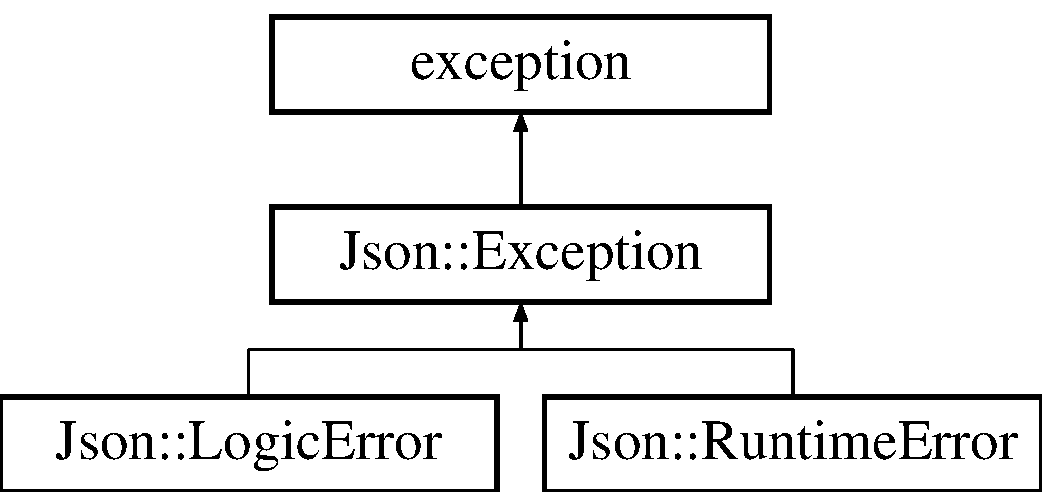
\includegraphics[height=3.000000cm]{classJson_1_1Exception}
\end{center}
\end{figure}
\subsection*{Public Member Functions}
\begin{DoxyCompactItemize}
\item 
\hyperlink{classJson_1_1Exception_ae764aa42e0755bd4ce9d303e2733fa8f}{Exception} (\hyperlink{json_8hpp_a1e723f95759de062585bc4a8fd3fa4be}{J\+S\+O\+N\+C\+P\+P\+\_\+\+S\+T\+R\+I\+NG} const \&msg)
\item 
\hyperlink{classJson_1_1Exception_ab104964e6e77fdfccc5d1a24327fffe0}{$\sim$\+Exception} () \hyperlink{json_8hpp_a824d6199c91488107e443226fa6022c5}{J\+S\+O\+N\+C\+P\+P\+\_\+\+O\+V\+E\+R\+R\+I\+DE}  throw ()
\item 
char const $\ast$ \hyperlink{classJson_1_1Exception_a5a9ed7d91b828b9be81706ef9d483ed6}{what} () const \hyperlink{json_8hpp_a824d6199c91488107e443226fa6022c5}{J\+S\+O\+N\+C\+P\+P\+\_\+\+O\+V\+E\+R\+R\+I\+DE}  throw ()
\end{DoxyCompactItemize}
\subsection*{Protected Attributes}
\begin{DoxyCompactItemize}
\item 
\hyperlink{json_8hpp_a1e723f95759de062585bc4a8fd3fa4be}{J\+S\+O\+N\+C\+P\+P\+\_\+\+S\+T\+R\+I\+NG} \hyperlink{classJson_1_1Exception_aae3cbb8b45bf21480f64502a8329659f}{msg\+\_\+}
\end{DoxyCompactItemize}


\subsection{Detailed Description}
Base class for all exceptions we throw. 

We use nothing but these internally. Of course, S\+TL can throw others. 

\subsection{Constructor \& Destructor Documentation}
\index{Json\+::\+Exception@{Json\+::\+Exception}!Exception@{Exception}}
\index{Exception@{Exception}!Json\+::\+Exception@{Json\+::\+Exception}}
\subsubsection[{\texorpdfstring{Exception(\+J\+S\+O\+N\+C\+P\+P\+\_\+\+S\+T\+R\+I\+N\+G const \&msg)}{Exception(JSONCPP_STRING const &msg)}}]{\setlength{\rightskip}{0pt plus 5cm}Json\+::\+Exception\+::\+Exception (
\begin{DoxyParamCaption}
\item[{{\bf J\+S\+O\+N\+C\+P\+P\+\_\+\+S\+T\+R\+I\+NG} const \&}]{msg}
\end{DoxyParamCaption}
)}\hypertarget{classJson_1_1Exception_ae764aa42e0755bd4ce9d303e2733fa8f}{}\label{classJson_1_1Exception_ae764aa42e0755bd4ce9d303e2733fa8f}
\index{Json\+::\+Exception@{Json\+::\+Exception}!````~Exception@{$\sim$\+Exception}}
\index{````~Exception@{$\sim$\+Exception}!Json\+::\+Exception@{Json\+::\+Exception}}
\subsubsection[{\texorpdfstring{$\sim$\+Exception() J\+S\+O\+N\+C\+P\+P\+\_\+\+O\+V\+E\+R\+R\+I\+DE}{~Exception() JSONCPP_OVERRIDE}}]{\setlength{\rightskip}{0pt plus 5cm}Json\+::\+Exception\+::$\sim$\+Exception (
\begin{DoxyParamCaption}
{}
\end{DoxyParamCaption}
) throw  ) }\hypertarget{classJson_1_1Exception_ab104964e6e77fdfccc5d1a24327fffe0}{}\label{classJson_1_1Exception_ab104964e6e77fdfccc5d1a24327fffe0}


\subsection{Member Function Documentation}
\index{Json\+::\+Exception@{Json\+::\+Exception}!what@{what}}
\index{what@{what}!Json\+::\+Exception@{Json\+::\+Exception}}
\subsubsection[{\texorpdfstring{what() const J\+S\+O\+N\+C\+P\+P\+\_\+\+O\+V\+E\+R\+R\+I\+DE}{what() const JSONCPP_OVERRIDE}}]{\setlength{\rightskip}{0pt plus 5cm}char const $\ast$ Json\+::\+Exception\+::what (
\begin{DoxyParamCaption}
{}
\end{DoxyParamCaption}
) const throw  ) }\hypertarget{classJson_1_1Exception_a5a9ed7d91b828b9be81706ef9d483ed6}{}\label{classJson_1_1Exception_a5a9ed7d91b828b9be81706ef9d483ed6}


\subsection{Member Data Documentation}
\index{Json\+::\+Exception@{Json\+::\+Exception}!msg\+\_\+@{msg\+\_\+}}
\index{msg\+\_\+@{msg\+\_\+}!Json\+::\+Exception@{Json\+::\+Exception}}
\subsubsection[{\texorpdfstring{msg\+\_\+}{msg_}}]{\setlength{\rightskip}{0pt plus 5cm}{\bf J\+S\+O\+N\+C\+P\+P\+\_\+\+S\+T\+R\+I\+NG} Json\+::\+Exception\+::msg\+\_\+\hspace{0.3cm}{\ttfamily [protected]}}\hypertarget{classJson_1_1Exception_aae3cbb8b45bf21480f64502a8329659f}{}\label{classJson_1_1Exception_aae3cbb8b45bf21480f64502a8329659f}


The documentation for this class was generated from the following files\+:\begin{DoxyCompactItemize}
\item 
/home/pranav/\+Repositories/zcm/include/\hyperlink{json_8hpp}{json.\+hpp}\item 
/home/pranav/\+Repositories/zcm/src/\hyperlink{json_8cpp}{json.\+cpp}\end{DoxyCompactItemize}

\hypertarget{classJson_1_1CharReader_1_1Factory}{}\section{Json\+:\+:Char\+Reader\+:\+:Factory Class Reference}
\label{classJson_1_1CharReader_1_1Factory}\index{Json\+::\+Char\+Reader\+::\+Factory@{Json\+::\+Char\+Reader\+::\+Factory}}


{\ttfamily \#include $<$json.\+hpp$>$}

Inheritance diagram for Json\+:\+:Char\+Reader\+:\+:Factory\+:\begin{figure}[H]
\begin{center}
\leavevmode
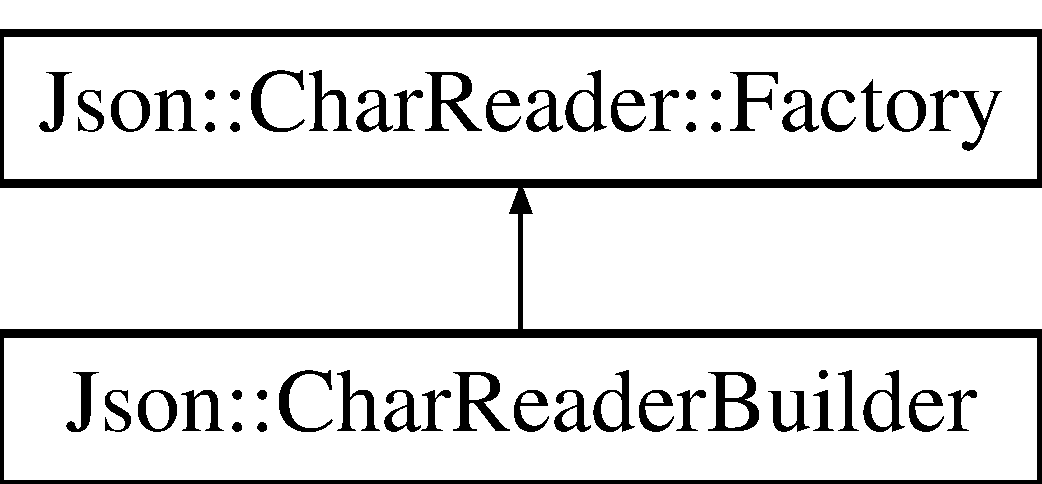
\includegraphics[height=2.000000cm]{classJson_1_1CharReader_1_1Factory}
\end{center}
\end{figure}
\subsection*{Public Member Functions}
\begin{DoxyCompactItemize}
\item 
virtual \hyperlink{classJson_1_1CharReader_1_1Factory_ae6938f632fa57f88e05818add5bc21be}{$\sim$\+Factory} ()
\item 
virtual \hyperlink{classJson_1_1CharReader}{Char\+Reader} $\ast$ \hyperlink{classJson_1_1CharReader_1_1Factory_a4c5862a1ffd432372dbe65cf59de98c4}{new\+Char\+Reader} () const =0
\begin{DoxyCompactList}\small\item\em Allocate a \hyperlink{classJson_1_1CharReader}{Char\+Reader} via operator new(). \end{DoxyCompactList}\end{DoxyCompactItemize}


\subsection{Constructor \& Destructor Documentation}
\index{Json\+::\+Char\+Reader\+::\+Factory@{Json\+::\+Char\+Reader\+::\+Factory}!````~Factory@{$\sim$\+Factory}}
\index{````~Factory@{$\sim$\+Factory}!Json\+::\+Char\+Reader\+::\+Factory@{Json\+::\+Char\+Reader\+::\+Factory}}
\subsubsection[{\texorpdfstring{$\sim$\+Factory()}{~Factory()}}]{\setlength{\rightskip}{0pt plus 5cm}virtual Json\+::\+Char\+Reader\+::\+Factory\+::$\sim$\+Factory (
\begin{DoxyParamCaption}
{}
\end{DoxyParamCaption}
)\hspace{0.3cm}{\ttfamily [inline]}, {\ttfamily [virtual]}}\hypertarget{classJson_1_1CharReader_1_1Factory_ae6938f632fa57f88e05818add5bc21be}{}\label{classJson_1_1CharReader_1_1Factory_ae6938f632fa57f88e05818add5bc21be}


\subsection{Member Function Documentation}
\index{Json\+::\+Char\+Reader\+::\+Factory@{Json\+::\+Char\+Reader\+::\+Factory}!new\+Char\+Reader@{new\+Char\+Reader}}
\index{new\+Char\+Reader@{new\+Char\+Reader}!Json\+::\+Char\+Reader\+::\+Factory@{Json\+::\+Char\+Reader\+::\+Factory}}
\subsubsection[{\texorpdfstring{new\+Char\+Reader() const =0}{newCharReader() const =0}}]{\setlength{\rightskip}{0pt plus 5cm}virtual {\bf Char\+Reader}$\ast$ Json\+::\+Char\+Reader\+::\+Factory\+::new\+Char\+Reader (
\begin{DoxyParamCaption}
{}
\end{DoxyParamCaption}
) const\hspace{0.3cm}{\ttfamily [pure virtual]}}\hypertarget{classJson_1_1CharReader_1_1Factory_a4c5862a1ffd432372dbe65cf59de98c4}{}\label{classJson_1_1CharReader_1_1Factory_a4c5862a1ffd432372dbe65cf59de98c4}


Allocate a \hyperlink{classJson_1_1CharReader}{Char\+Reader} via operator new(). 


\begin{DoxyExceptions}{Exceptions}
{\em std\+::exception} & if something goes wrong (e.\+g. invalid settings) \\
\hline
\end{DoxyExceptions}


Implemented in \hyperlink{classJson_1_1CharReaderBuilder_a3a262fcc76c1eb8eebfd4718fb4e9722}{Json\+::\+Char\+Reader\+Builder}.



The documentation for this class was generated from the following file\+:\begin{DoxyCompactItemize}
\item 
/home/pranav/\+Repositories/zcm/include/\hyperlink{json_8hpp}{json.\+hpp}\end{DoxyCompactItemize}

\hypertarget{classJson_1_1StreamWriter_1_1Factory}{}\section{Json\+:\+:Stream\+Writer\+:\+:Factory Class Reference}
\label{classJson_1_1StreamWriter_1_1Factory}\index{Json\+::\+Stream\+Writer\+::\+Factory@{Json\+::\+Stream\+Writer\+::\+Factory}}


A simple abstract factory.  




{\ttfamily \#include $<$json.\+hpp$>$}

Inheritance diagram for Json\+:\+:Stream\+Writer\+:\+:Factory\+:\begin{figure}[H]
\begin{center}
\leavevmode
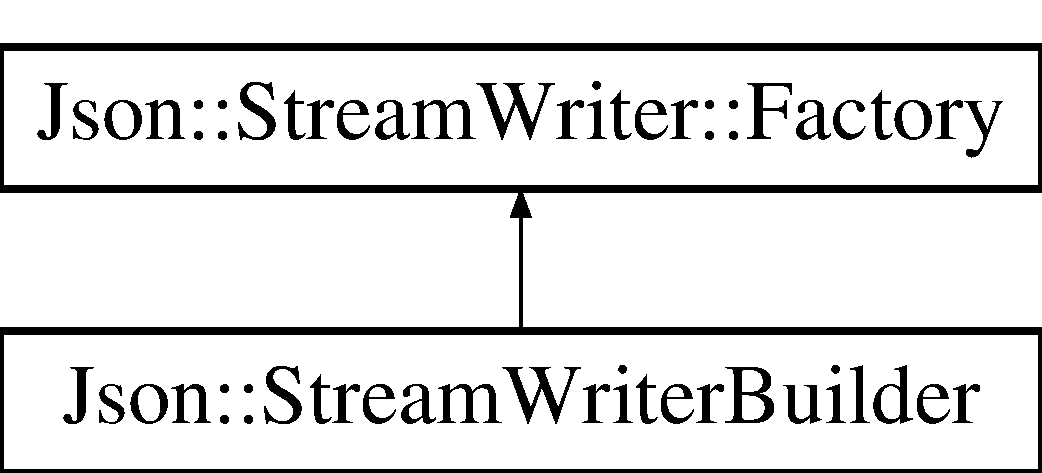
\includegraphics[height=2.000000cm]{classJson_1_1StreamWriter_1_1Factory}
\end{center}
\end{figure}
\subsection*{Public Member Functions}
\begin{DoxyCompactItemize}
\item 
virtual \hyperlink{classJson_1_1StreamWriter_1_1Factory_ad334ad5e81e3b9b1768620a446366ff1}{$\sim$\+Factory} ()
\item 
virtual \hyperlink{classJson_1_1StreamWriter}{Stream\+Writer} $\ast$ \hyperlink{classJson_1_1StreamWriter_1_1Factory_a9d30ec53e8288cd53befccf1009c5f31}{new\+Stream\+Writer} () const =0
\begin{DoxyCompactList}\small\item\em Allocate a \hyperlink{classJson_1_1CharReader}{Char\+Reader} via operator new(). \end{DoxyCompactList}\end{DoxyCompactItemize}


\subsection{Detailed Description}
A simple abstract factory. 

\subsection{Constructor \& Destructor Documentation}
\index{Json\+::\+Stream\+Writer\+::\+Factory@{Json\+::\+Stream\+Writer\+::\+Factory}!````~Factory@{$\sim$\+Factory}}
\index{````~Factory@{$\sim$\+Factory}!Json\+::\+Stream\+Writer\+::\+Factory@{Json\+::\+Stream\+Writer\+::\+Factory}}
\subsubsection[{\texorpdfstring{$\sim$\+Factory()}{~Factory()}}]{\setlength{\rightskip}{0pt plus 5cm}Json\+::\+Stream\+Writer\+::\+Factory\+::$\sim$\+Factory (
\begin{DoxyParamCaption}
{}
\end{DoxyParamCaption}
)\hspace{0.3cm}{\ttfamily [virtual]}}\hypertarget{classJson_1_1StreamWriter_1_1Factory_ad334ad5e81e3b9b1768620a446366ff1}{}\label{classJson_1_1StreamWriter_1_1Factory_ad334ad5e81e3b9b1768620a446366ff1}


\subsection{Member Function Documentation}
\index{Json\+::\+Stream\+Writer\+::\+Factory@{Json\+::\+Stream\+Writer\+::\+Factory}!new\+Stream\+Writer@{new\+Stream\+Writer}}
\index{new\+Stream\+Writer@{new\+Stream\+Writer}!Json\+::\+Stream\+Writer\+::\+Factory@{Json\+::\+Stream\+Writer\+::\+Factory}}
\subsubsection[{\texorpdfstring{new\+Stream\+Writer() const =0}{newStreamWriter() const =0}}]{\setlength{\rightskip}{0pt plus 5cm}virtual {\bf Stream\+Writer}$\ast$ Json\+::\+Stream\+Writer\+::\+Factory\+::new\+Stream\+Writer (
\begin{DoxyParamCaption}
{}
\end{DoxyParamCaption}
) const\hspace{0.3cm}{\ttfamily [pure virtual]}}\hypertarget{classJson_1_1StreamWriter_1_1Factory_a9d30ec53e8288cd53befccf1009c5f31}{}\label{classJson_1_1StreamWriter_1_1Factory_a9d30ec53e8288cd53befccf1009c5f31}


Allocate a \hyperlink{classJson_1_1CharReader}{Char\+Reader} via operator new(). 


\begin{DoxyExceptions}{Exceptions}
{\em std\+::exception} & if something goes wrong (e.\+g. invalid settings) \\
\hline
\end{DoxyExceptions}


Implemented in \hyperlink{classJson_1_1StreamWriterBuilder_ab9ee278609f88ae04a7c1a84e1f559e6}{Json\+::\+Stream\+Writer\+Builder}.



The documentation for this class was generated from the following files\+:\begin{DoxyCompactItemize}
\item 
/home/pranav/\+Repositories/zcm/include/\hyperlink{json_8hpp}{json.\+hpp}\item 
/home/pranav/\+Repositories/zcm/src/\hyperlink{json_8cpp}{json.\+cpp}\end{DoxyCompactItemize}

\hypertarget{classJson_1_1FastWriter}{}\section{Json\+:\+:Fast\+Writer Class Reference}
\label{classJson_1_1FastWriter}\index{Json\+::\+Fast\+Writer@{Json\+::\+Fast\+Writer}}


Outputs a \hyperlink{classJson_1_1Value}{Value} in \href{http://www.json.org}{\tt J\+S\+ON} format without formatting (not human friendly).  




{\ttfamily \#include $<$json.\+hpp$>$}

Inheritance diagram for Json\+:\+:Fast\+Writer\+:\begin{figure}[H]
\begin{center}
\leavevmode
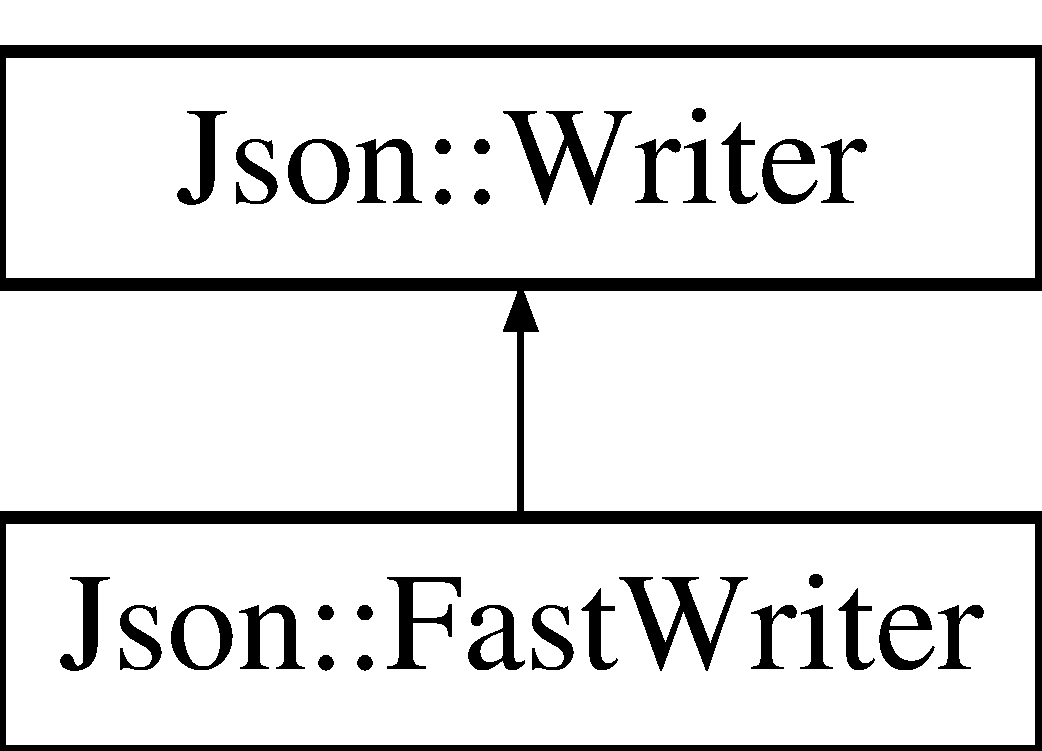
\includegraphics[height=2.000000cm]{classJson_1_1FastWriter}
\end{center}
\end{figure}
\subsection*{Public Member Functions}
\begin{DoxyCompactItemize}
\item 
\hyperlink{classJson_1_1FastWriter_a1bbc73ce1a1cc7b09cd1e02db3905170}{Fast\+Writer} ()
\item 
\hyperlink{classJson_1_1FastWriter_a34152eac509fe00c9b2e15ce2fc94ab8}{$\sim$\+Fast\+Writer} () \hyperlink{json_8hpp_a824d6199c91488107e443226fa6022c5}{J\+S\+O\+N\+C\+P\+P\+\_\+\+O\+V\+E\+R\+R\+I\+DE}
\item 
void \hyperlink{classJson_1_1FastWriter_a78d98e9f76d33660ad6e6a1abe287d45}{enable\+Y\+A\+M\+L\+Compatibility} ()
\item 
void \hyperlink{classJson_1_1FastWriter_a6e93d8dce951e408517311026a065b40}{drop\+Null\+Placeholders} ()
\begin{DoxyCompactList}\small\item\em Drop the \char`\"{}null\char`\"{} string from the writer\textquotesingle{}s output for null\+Values. \end{DoxyCompactList}\item 
void \hyperlink{classJson_1_1FastWriter_af4ee077d365d75941fb2688d97207a55}{omit\+Ending\+Line\+Feed} ()
\item 
\hyperlink{json_8hpp_a1e723f95759de062585bc4a8fd3fa4be}{J\+S\+O\+N\+C\+P\+P\+\_\+\+S\+T\+R\+I\+NG} \hyperlink{classJson_1_1FastWriter_a93d45ba4bc312371d08beb3e3dfbe654}{write} (const \hyperlink{classJson_1_1Value}{Value} \&root) \hyperlink{json_8hpp_a824d6199c91488107e443226fa6022c5}{J\+S\+O\+N\+C\+P\+P\+\_\+\+O\+V\+E\+R\+R\+I\+DE}
\end{DoxyCompactItemize}
\subsection*{Private Member Functions}
\begin{DoxyCompactItemize}
\item 
void \hyperlink{classJson_1_1FastWriter_a2ef4a2ce13a341171f01f414f4fdd765}{write\+Value} (const \hyperlink{classJson_1_1Value}{Value} \&value)
\end{DoxyCompactItemize}
\subsection*{Private Attributes}
\begin{DoxyCompactItemize}
\item 
\hyperlink{json_8hpp_a1e723f95759de062585bc4a8fd3fa4be}{J\+S\+O\+N\+C\+P\+P\+\_\+\+S\+T\+R\+I\+NG} \hyperlink{classJson_1_1FastWriter_a5e08c44579db8704dba1ebe37d39fdba}{document\+\_\+}
\item 
bool \hyperlink{classJson_1_1FastWriter_a4c4c1911179bf472d24492915b0e489a}{yaml\+Compatiblity\+Enabled\+\_\+}
\item 
bool \hyperlink{classJson_1_1FastWriter_a97e9d4ff84b59a48756dcc27a71b5904}{drop\+Null\+Placeholders\+\_\+}
\item 
bool \hyperlink{classJson_1_1FastWriter_abd6e13851db6dcf59d84af68d48d50ac}{omit\+Ending\+Line\+Feed\+\_\+}
\end{DoxyCompactItemize}


\subsection{Detailed Description}
Outputs a \hyperlink{classJson_1_1Value}{Value} in \href{http://www.json.org}{\tt J\+S\+ON} format without formatting (not human friendly). 

The J\+S\+ON document is written in a single line. It is not intended for \textquotesingle{}human\textquotesingle{} consumption, but may be usefull to support feature such as R\+PC where bandwith is limited. \begin{DoxySeeAlso}{See also}
\hyperlink{classJson_1_1Reader}{Reader}, \hyperlink{classJson_1_1Value}{Value} 
\end{DoxySeeAlso}
\begin{DoxyRefDesc}{Deprecated}
\item[\hyperlink{deprecated__deprecated000008}{Deprecated}]Use \hyperlink{classJson_1_1StreamWriterBuilder}{Stream\+Writer\+Builder}. \end{DoxyRefDesc}


\subsection{Constructor \& Destructor Documentation}
\index{Json\+::\+Fast\+Writer@{Json\+::\+Fast\+Writer}!Fast\+Writer@{Fast\+Writer}}
\index{Fast\+Writer@{Fast\+Writer}!Json\+::\+Fast\+Writer@{Json\+::\+Fast\+Writer}}
\subsubsection[{\texorpdfstring{Fast\+Writer()}{FastWriter()}}]{\setlength{\rightskip}{0pt plus 5cm}Json\+::\+Fast\+Writer\+::\+Fast\+Writer (
\begin{DoxyParamCaption}
{}
\end{DoxyParamCaption}
)}\hypertarget{classJson_1_1FastWriter_a1bbc73ce1a1cc7b09cd1e02db3905170}{}\label{classJson_1_1FastWriter_a1bbc73ce1a1cc7b09cd1e02db3905170}
\index{Json\+::\+Fast\+Writer@{Json\+::\+Fast\+Writer}!````~Fast\+Writer@{$\sim$\+Fast\+Writer}}
\index{````~Fast\+Writer@{$\sim$\+Fast\+Writer}!Json\+::\+Fast\+Writer@{Json\+::\+Fast\+Writer}}
\subsubsection[{\texorpdfstring{$\sim$\+Fast\+Writer() J\+S\+O\+N\+C\+P\+P\+\_\+\+O\+V\+E\+R\+R\+I\+DE}{~FastWriter() JSONCPP_OVERRIDE}}]{\setlength{\rightskip}{0pt plus 5cm}Json\+::\+Fast\+Writer\+::$\sim$\+Fast\+Writer (
\begin{DoxyParamCaption}
{}
\end{DoxyParamCaption}
)\hspace{0.3cm}{\ttfamily [inline]}}\hypertarget{classJson_1_1FastWriter_a34152eac509fe00c9b2e15ce2fc94ab8}{}\label{classJson_1_1FastWriter_a34152eac509fe00c9b2e15ce2fc94ab8}


\subsection{Member Function Documentation}
\index{Json\+::\+Fast\+Writer@{Json\+::\+Fast\+Writer}!drop\+Null\+Placeholders@{drop\+Null\+Placeholders}}
\index{drop\+Null\+Placeholders@{drop\+Null\+Placeholders}!Json\+::\+Fast\+Writer@{Json\+::\+Fast\+Writer}}
\subsubsection[{\texorpdfstring{drop\+Null\+Placeholders()}{dropNullPlaceholders()}}]{\setlength{\rightskip}{0pt plus 5cm}void Json\+::\+Fast\+Writer\+::drop\+Null\+Placeholders (
\begin{DoxyParamCaption}
{}
\end{DoxyParamCaption}
)}\hypertarget{classJson_1_1FastWriter_a6e93d8dce951e408517311026a065b40}{}\label{classJson_1_1FastWriter_a6e93d8dce951e408517311026a065b40}


Drop the \char`\"{}null\char`\"{} string from the writer\textquotesingle{}s output for null\+Values. 

Strictly speaking, this is not valid J\+S\+ON. But when the output is being fed to a browser\textquotesingle{}s Javascript, it makes for smaller output and the browser can handle the output just fine. \index{Json\+::\+Fast\+Writer@{Json\+::\+Fast\+Writer}!enable\+Y\+A\+M\+L\+Compatibility@{enable\+Y\+A\+M\+L\+Compatibility}}
\index{enable\+Y\+A\+M\+L\+Compatibility@{enable\+Y\+A\+M\+L\+Compatibility}!Json\+::\+Fast\+Writer@{Json\+::\+Fast\+Writer}}
\subsubsection[{\texorpdfstring{enable\+Y\+A\+M\+L\+Compatibility()}{enableYAMLCompatibility()}}]{\setlength{\rightskip}{0pt plus 5cm}void Json\+::\+Fast\+Writer\+::enable\+Y\+A\+M\+L\+Compatibility (
\begin{DoxyParamCaption}
{}
\end{DoxyParamCaption}
)}\hypertarget{classJson_1_1FastWriter_a78d98e9f76d33660ad6e6a1abe287d45}{}\label{classJson_1_1FastWriter_a78d98e9f76d33660ad6e6a1abe287d45}
\index{Json\+::\+Fast\+Writer@{Json\+::\+Fast\+Writer}!omit\+Ending\+Line\+Feed@{omit\+Ending\+Line\+Feed}}
\index{omit\+Ending\+Line\+Feed@{omit\+Ending\+Line\+Feed}!Json\+::\+Fast\+Writer@{Json\+::\+Fast\+Writer}}
\subsubsection[{\texorpdfstring{omit\+Ending\+Line\+Feed()}{omitEndingLineFeed()}}]{\setlength{\rightskip}{0pt plus 5cm}void Json\+::\+Fast\+Writer\+::omit\+Ending\+Line\+Feed (
\begin{DoxyParamCaption}
{}
\end{DoxyParamCaption}
)}\hypertarget{classJson_1_1FastWriter_af4ee077d365d75941fb2688d97207a55}{}\label{classJson_1_1FastWriter_af4ee077d365d75941fb2688d97207a55}
\index{Json\+::\+Fast\+Writer@{Json\+::\+Fast\+Writer}!write@{write}}
\index{write@{write}!Json\+::\+Fast\+Writer@{Json\+::\+Fast\+Writer}}
\subsubsection[{\texorpdfstring{write(const Value \&root) J\+S\+O\+N\+C\+P\+P\+\_\+\+O\+V\+E\+R\+R\+I\+DE}{write(const Value &root) JSONCPP_OVERRIDE}}]{\setlength{\rightskip}{0pt plus 5cm}{\bf J\+S\+O\+N\+C\+P\+P\+\_\+\+S\+T\+R\+I\+NG} Json\+::\+Fast\+Writer\+::write (
\begin{DoxyParamCaption}
\item[{const {\bf Value} \&}]{root}
\end{DoxyParamCaption}
)\hspace{0.3cm}{\ttfamily [virtual]}}\hypertarget{classJson_1_1FastWriter_a93d45ba4bc312371d08beb3e3dfbe654}{}\label{classJson_1_1FastWriter_a93d45ba4bc312371d08beb3e3dfbe654}


Implements \hyperlink{classJson_1_1Writer_a61c55882b82c7651d0b9b683c6d3f371}{Json\+::\+Writer}.

\index{Json\+::\+Fast\+Writer@{Json\+::\+Fast\+Writer}!write\+Value@{write\+Value}}
\index{write\+Value@{write\+Value}!Json\+::\+Fast\+Writer@{Json\+::\+Fast\+Writer}}
\subsubsection[{\texorpdfstring{write\+Value(const Value \&value)}{writeValue(const Value &value)}}]{\setlength{\rightskip}{0pt plus 5cm}void Json\+::\+Fast\+Writer\+::write\+Value (
\begin{DoxyParamCaption}
\item[{const {\bf Value} \&}]{value}
\end{DoxyParamCaption}
)\hspace{0.3cm}{\ttfamily [private]}}\hypertarget{classJson_1_1FastWriter_a2ef4a2ce13a341171f01f414f4fdd765}{}\label{classJson_1_1FastWriter_a2ef4a2ce13a341171f01f414f4fdd765}


\subsection{Member Data Documentation}
\index{Json\+::\+Fast\+Writer@{Json\+::\+Fast\+Writer}!document\+\_\+@{document\+\_\+}}
\index{document\+\_\+@{document\+\_\+}!Json\+::\+Fast\+Writer@{Json\+::\+Fast\+Writer}}
\subsubsection[{\texorpdfstring{document\+\_\+}{document_}}]{\setlength{\rightskip}{0pt plus 5cm}{\bf J\+S\+O\+N\+C\+P\+P\+\_\+\+S\+T\+R\+I\+NG} Json\+::\+Fast\+Writer\+::document\+\_\+\hspace{0.3cm}{\ttfamily [private]}}\hypertarget{classJson_1_1FastWriter_a5e08c44579db8704dba1ebe37d39fdba}{}\label{classJson_1_1FastWriter_a5e08c44579db8704dba1ebe37d39fdba}
\index{Json\+::\+Fast\+Writer@{Json\+::\+Fast\+Writer}!drop\+Null\+Placeholders\+\_\+@{drop\+Null\+Placeholders\+\_\+}}
\index{drop\+Null\+Placeholders\+\_\+@{drop\+Null\+Placeholders\+\_\+}!Json\+::\+Fast\+Writer@{Json\+::\+Fast\+Writer}}
\subsubsection[{\texorpdfstring{drop\+Null\+Placeholders\+\_\+}{dropNullPlaceholders_}}]{\setlength{\rightskip}{0pt plus 5cm}bool Json\+::\+Fast\+Writer\+::drop\+Null\+Placeholders\+\_\+\hspace{0.3cm}{\ttfamily [private]}}\hypertarget{classJson_1_1FastWriter_a97e9d4ff84b59a48756dcc27a71b5904}{}\label{classJson_1_1FastWriter_a97e9d4ff84b59a48756dcc27a71b5904}
\index{Json\+::\+Fast\+Writer@{Json\+::\+Fast\+Writer}!omit\+Ending\+Line\+Feed\+\_\+@{omit\+Ending\+Line\+Feed\+\_\+}}
\index{omit\+Ending\+Line\+Feed\+\_\+@{omit\+Ending\+Line\+Feed\+\_\+}!Json\+::\+Fast\+Writer@{Json\+::\+Fast\+Writer}}
\subsubsection[{\texorpdfstring{omit\+Ending\+Line\+Feed\+\_\+}{omitEndingLineFeed_}}]{\setlength{\rightskip}{0pt plus 5cm}bool Json\+::\+Fast\+Writer\+::omit\+Ending\+Line\+Feed\+\_\+\hspace{0.3cm}{\ttfamily [private]}}\hypertarget{classJson_1_1FastWriter_abd6e13851db6dcf59d84af68d48d50ac}{}\label{classJson_1_1FastWriter_abd6e13851db6dcf59d84af68d48d50ac}
\index{Json\+::\+Fast\+Writer@{Json\+::\+Fast\+Writer}!yaml\+Compatiblity\+Enabled\+\_\+@{yaml\+Compatiblity\+Enabled\+\_\+}}
\index{yaml\+Compatiblity\+Enabled\+\_\+@{yaml\+Compatiblity\+Enabled\+\_\+}!Json\+::\+Fast\+Writer@{Json\+::\+Fast\+Writer}}
\subsubsection[{\texorpdfstring{yaml\+Compatiblity\+Enabled\+\_\+}{yamlCompatiblityEnabled_}}]{\setlength{\rightskip}{0pt plus 5cm}bool Json\+::\+Fast\+Writer\+::yaml\+Compatiblity\+Enabled\+\_\+\hspace{0.3cm}{\ttfamily [private]}}\hypertarget{classJson_1_1FastWriter_a4c4c1911179bf472d24492915b0e489a}{}\label{classJson_1_1FastWriter_a4c4c1911179bf472d24492915b0e489a}


The documentation for this class was generated from the following files\+:\begin{DoxyCompactItemize}
\item 
/home/pranav/\+Repositories/zcm/include/\hyperlink{json_8hpp}{json.\+hpp}\item 
/home/pranav/\+Repositories/zcm/src/\hyperlink{json_8cpp}{json.\+cpp}\end{DoxyCompactItemize}

\hypertarget{classJson_1_1Features}{}\section{Json\+:\+:Features Class Reference}
\label{classJson_1_1Features}\index{Json\+::\+Features@{Json\+::\+Features}}


Configuration passed to reader and writer.  




{\ttfamily \#include $<$json.\+hpp$>$}

\subsection*{Public Member Functions}
\begin{DoxyCompactItemize}
\item 
\hyperlink{classJson_1_1Features_ad15a091cb61bb31323299a95970d2644}{Features} ()
\begin{DoxyCompactList}\small\item\em Initialize the configuration like Json\+Config\+::all\+Features;. \end{DoxyCompactList}\end{DoxyCompactItemize}
\subsection*{Static Public Member Functions}
\begin{DoxyCompactItemize}
\item 
static \hyperlink{classJson_1_1Features}{Features} \hyperlink{classJson_1_1Features_a63894da6e2c100b38741fa933f3d33ae}{all} ()
\begin{DoxyCompactList}\small\item\em A configuration that allows all features and assumes all strings are U\+T\+F-\/8. \end{DoxyCompactList}\item 
static \hyperlink{classJson_1_1Features}{Features} \hyperlink{classJson_1_1Features_ae23176c14b2e79e81fb61fb1a8ab58ee}{strict\+Mode} ()
\begin{DoxyCompactList}\small\item\em A configuration that is strictly compatible with the J\+S\+ON specification. \end{DoxyCompactList}\end{DoxyCompactItemize}
\subsection*{Public Attributes}
\begin{DoxyCompactItemize}
\item 
bool \hyperlink{classJson_1_1Features_a33afd389719624b6bdb23950b3c346c9}{allow\+Comments\+\_\+}
\begin{DoxyCompactList}\small\item\em {\ttfamily true} if comments are allowed. Default\+: {\ttfamily true}. \end{DoxyCompactList}\item 
bool \hyperlink{classJson_1_1Features_a1162c37a1458adc32582b585b552f9c3}{strict\+Root\+\_\+}
\begin{DoxyCompactList}\small\item\em {\ttfamily true} if root must be either an array or an object value. \end{DoxyCompactList}\item 
bool \hyperlink{classJson_1_1Features_a5076aa72c05c7596ac339ede36c97a6a}{allow\+Dropped\+Null\+Placeholders\+\_\+}
\begin{DoxyCompactList}\small\item\em {\ttfamily true} if dropped null placeholders are allowed. Default\+: {\ttfamily false}. \end{DoxyCompactList}\item 
bool \hyperlink{classJson_1_1Features_aff3cb16b79d15d3d761b11a0dd6d4d6b}{allow\+Numeric\+Keys\+\_\+}
\begin{DoxyCompactList}\small\item\em {\ttfamily true} if numeric object key are allowed. Default\+: {\ttfamily false}. \end{DoxyCompactList}\end{DoxyCompactItemize}


\subsection{Detailed Description}
Configuration passed to reader and writer. 

This configuration object can be used to force the \hyperlink{classJson_1_1Reader}{Reader} or \hyperlink{classJson_1_1Writer}{Writer} to behave in a standard conforming way. 

\subsection{Constructor \& Destructor Documentation}
\index{Json\+::\+Features@{Json\+::\+Features}!Features@{Features}}
\index{Features@{Features}!Json\+::\+Features@{Json\+::\+Features}}
\subsubsection[{\texorpdfstring{Features()}{Features()}}]{\setlength{\rightskip}{0pt plus 5cm}Json\+::\+Features\+::\+Features (
\begin{DoxyParamCaption}
{}
\end{DoxyParamCaption}
)}\hypertarget{classJson_1_1Features_ad15a091cb61bb31323299a95970d2644}{}\label{classJson_1_1Features_ad15a091cb61bb31323299a95970d2644}


Initialize the configuration like Json\+Config\+::all\+Features;. 



\subsection{Member Function Documentation}
\index{Json\+::\+Features@{Json\+::\+Features}!all@{all}}
\index{all@{all}!Json\+::\+Features@{Json\+::\+Features}}
\subsubsection[{\texorpdfstring{all()}{all()}}]{\setlength{\rightskip}{0pt plus 5cm}{\bf Features} Json\+::\+Features\+::all (
\begin{DoxyParamCaption}
{}
\end{DoxyParamCaption}
)\hspace{0.3cm}{\ttfamily [static]}}\hypertarget{classJson_1_1Features_a63894da6e2c100b38741fa933f3d33ae}{}\label{classJson_1_1Features_a63894da6e2c100b38741fa933f3d33ae}


A configuration that allows all features and assumes all strings are U\+T\+F-\/8. 


\begin{DoxyItemize}
\item C \& C++ comments are allowed
\item Root object can be any J\+S\+ON value
\item Assumes \hyperlink{classJson_1_1Value}{Value} strings are encoded in U\+T\+F-\/8 
\end{DoxyItemize}\index{Json\+::\+Features@{Json\+::\+Features}!strict\+Mode@{strict\+Mode}}
\index{strict\+Mode@{strict\+Mode}!Json\+::\+Features@{Json\+::\+Features}}
\subsubsection[{\texorpdfstring{strict\+Mode()}{strictMode()}}]{\setlength{\rightskip}{0pt plus 5cm}{\bf Features} Json\+::\+Features\+::strict\+Mode (
\begin{DoxyParamCaption}
{}
\end{DoxyParamCaption}
)\hspace{0.3cm}{\ttfamily [static]}}\hypertarget{classJson_1_1Features_ae23176c14b2e79e81fb61fb1a8ab58ee}{}\label{classJson_1_1Features_ae23176c14b2e79e81fb61fb1a8ab58ee}


A configuration that is strictly compatible with the J\+S\+ON specification. 


\begin{DoxyItemize}
\item Comments are forbidden.
\item Root object must be either an array or an object value.
\item Assumes \hyperlink{classJson_1_1Value}{Value} strings are encoded in U\+T\+F-\/8 
\end{DoxyItemize}

\subsection{Member Data Documentation}
\index{Json\+::\+Features@{Json\+::\+Features}!allow\+Comments\+\_\+@{allow\+Comments\+\_\+}}
\index{allow\+Comments\+\_\+@{allow\+Comments\+\_\+}!Json\+::\+Features@{Json\+::\+Features}}
\subsubsection[{\texorpdfstring{allow\+Comments\+\_\+}{allowComments_}}]{\setlength{\rightskip}{0pt plus 5cm}bool Json\+::\+Features\+::allow\+Comments\+\_\+}\hypertarget{classJson_1_1Features_a33afd389719624b6bdb23950b3c346c9}{}\label{classJson_1_1Features_a33afd389719624b6bdb23950b3c346c9}


{\ttfamily true} if comments are allowed. Default\+: {\ttfamily true}. 

\index{Json\+::\+Features@{Json\+::\+Features}!allow\+Dropped\+Null\+Placeholders\+\_\+@{allow\+Dropped\+Null\+Placeholders\+\_\+}}
\index{allow\+Dropped\+Null\+Placeholders\+\_\+@{allow\+Dropped\+Null\+Placeholders\+\_\+}!Json\+::\+Features@{Json\+::\+Features}}
\subsubsection[{\texorpdfstring{allow\+Dropped\+Null\+Placeholders\+\_\+}{allowDroppedNullPlaceholders_}}]{\setlength{\rightskip}{0pt plus 5cm}bool Json\+::\+Features\+::allow\+Dropped\+Null\+Placeholders\+\_\+}\hypertarget{classJson_1_1Features_a5076aa72c05c7596ac339ede36c97a6a}{}\label{classJson_1_1Features_a5076aa72c05c7596ac339ede36c97a6a}


{\ttfamily true} if dropped null placeholders are allowed. Default\+: {\ttfamily false}. 

\index{Json\+::\+Features@{Json\+::\+Features}!allow\+Numeric\+Keys\+\_\+@{allow\+Numeric\+Keys\+\_\+}}
\index{allow\+Numeric\+Keys\+\_\+@{allow\+Numeric\+Keys\+\_\+}!Json\+::\+Features@{Json\+::\+Features}}
\subsubsection[{\texorpdfstring{allow\+Numeric\+Keys\+\_\+}{allowNumericKeys_}}]{\setlength{\rightskip}{0pt plus 5cm}bool Json\+::\+Features\+::allow\+Numeric\+Keys\+\_\+}\hypertarget{classJson_1_1Features_aff3cb16b79d15d3d761b11a0dd6d4d6b}{}\label{classJson_1_1Features_aff3cb16b79d15d3d761b11a0dd6d4d6b}


{\ttfamily true} if numeric object key are allowed. Default\+: {\ttfamily false}. 

\index{Json\+::\+Features@{Json\+::\+Features}!strict\+Root\+\_\+@{strict\+Root\+\_\+}}
\index{strict\+Root\+\_\+@{strict\+Root\+\_\+}!Json\+::\+Features@{Json\+::\+Features}}
\subsubsection[{\texorpdfstring{strict\+Root\+\_\+}{strictRoot_}}]{\setlength{\rightskip}{0pt plus 5cm}bool Json\+::\+Features\+::strict\+Root\+\_\+}\hypertarget{classJson_1_1Features_a1162c37a1458adc32582b585b552f9c3}{}\label{classJson_1_1Features_a1162c37a1458adc32582b585b552f9c3}


{\ttfamily true} if root must be either an array or an object value. 

Default\+: {\ttfamily false}. 

The documentation for this class was generated from the following files\+:\begin{DoxyCompactItemize}
\item 
/home/pranav/\+Repositories/zcm/include/\hyperlink{json_8hpp}{json.\+hpp}\item 
/home/pranav/\+Repositories/zcm/src/\hyperlink{json_8cpp}{json.\+cpp}\end{DoxyCompactItemize}

\hypertarget{classJson_1_1LogicError}{}\section{Json\+:\+:Logic\+Error Class Reference}
\label{classJson_1_1LogicError}\index{Json\+::\+Logic\+Error@{Json\+::\+Logic\+Error}}


Exceptions thrown by J\+S\+O\+N\+\_\+\+A\+S\+S\+E\+R\+T/\+J\+S\+O\+N\+\_\+\+F\+A\+IL macros.  




{\ttfamily \#include $<$json.\+hpp$>$}

Inheritance diagram for Json\+:\+:Logic\+Error\+:\begin{figure}[H]
\begin{center}
\leavevmode
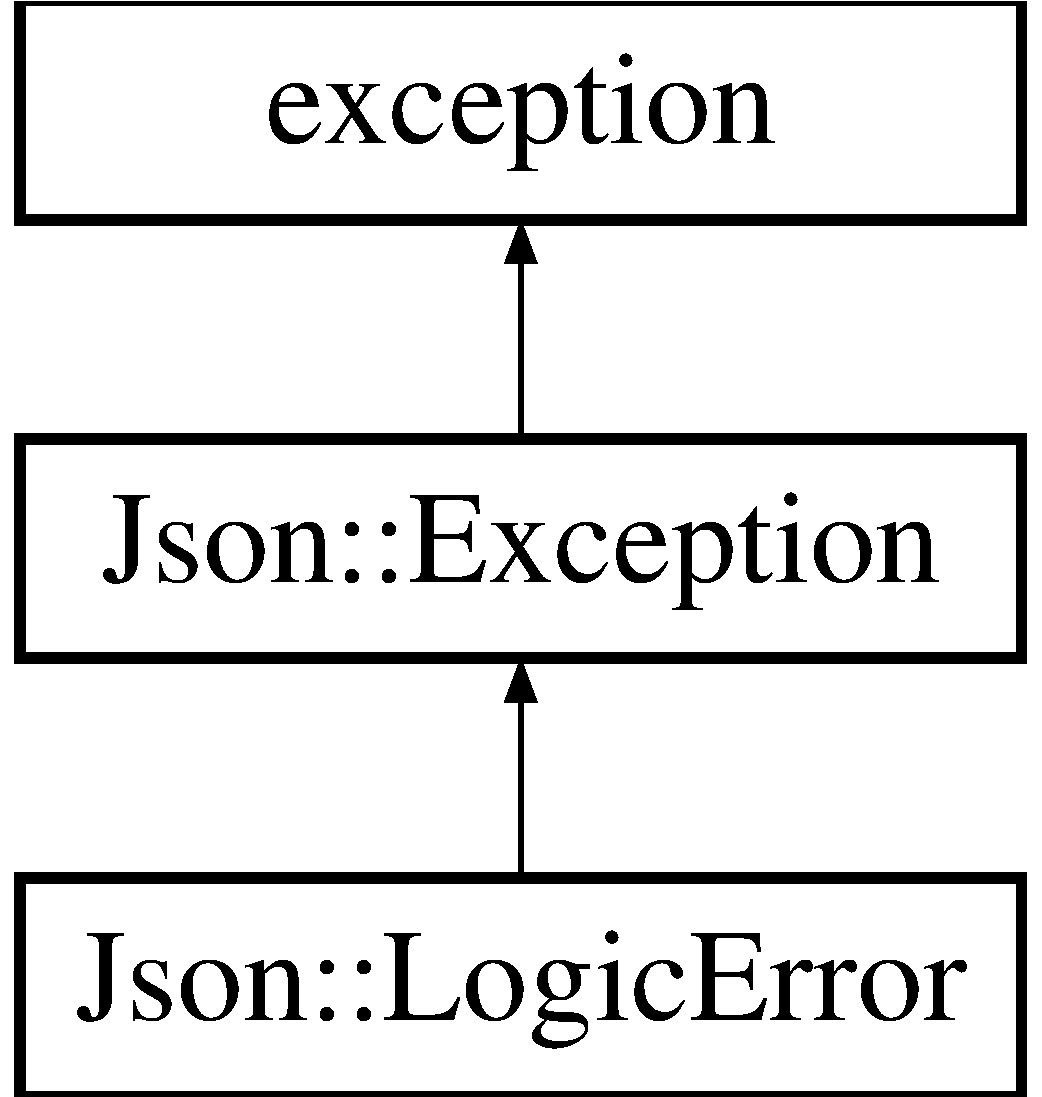
\includegraphics[height=3.000000cm]{classJson_1_1LogicError}
\end{center}
\end{figure}
\subsection*{Public Member Functions}
\begin{DoxyCompactItemize}
\item 
\hyperlink{classJson_1_1LogicError_acca679aa49768a4a1de7b705c67c2919}{Logic\+Error} (\hyperlink{json_8hpp_a1e723f95759de062585bc4a8fd3fa4be}{J\+S\+O\+N\+C\+P\+P\+\_\+\+S\+T\+R\+I\+NG} const \&msg)
\item 
char const $\ast$ \hyperlink{classJson_1_1Exception_a5a9ed7d91b828b9be81706ef9d483ed6}{what} () const \hyperlink{json_8hpp_a824d6199c91488107e443226fa6022c5}{J\+S\+O\+N\+C\+P\+P\+\_\+\+O\+V\+E\+R\+R\+I\+DE}  throw ()
\end{DoxyCompactItemize}
\subsection*{Protected Attributes}
\begin{DoxyCompactItemize}
\item 
\hyperlink{json_8hpp_a1e723f95759de062585bc4a8fd3fa4be}{J\+S\+O\+N\+C\+P\+P\+\_\+\+S\+T\+R\+I\+NG} \hyperlink{classJson_1_1Exception_aae3cbb8b45bf21480f64502a8329659f}{msg\+\_\+}
\end{DoxyCompactItemize}


\subsection{Detailed Description}
Exceptions thrown by J\+S\+O\+N\+\_\+\+A\+S\+S\+E\+R\+T/\+J\+S\+O\+N\+\_\+\+F\+A\+IL macros. 

These are precondition-\/violations (user bugs) and internal errors (our bugs).

\begin{DoxyRemark}{Remarks}
derived from \hyperlink{classJson_1_1Exception}{Json\+::\+Exception} 
\end{DoxyRemark}


\subsection{Constructor \& Destructor Documentation}
\index{Json\+::\+Logic\+Error@{Json\+::\+Logic\+Error}!Logic\+Error@{Logic\+Error}}
\index{Logic\+Error@{Logic\+Error}!Json\+::\+Logic\+Error@{Json\+::\+Logic\+Error}}
\subsubsection[{\texorpdfstring{Logic\+Error(\+J\+S\+O\+N\+C\+P\+P\+\_\+\+S\+T\+R\+I\+N\+G const \&msg)}{LogicError(JSONCPP_STRING const &msg)}}]{\setlength{\rightskip}{0pt plus 5cm}Json\+::\+Logic\+Error\+::\+Logic\+Error (
\begin{DoxyParamCaption}
\item[{{\bf J\+S\+O\+N\+C\+P\+P\+\_\+\+S\+T\+R\+I\+NG} const \&}]{msg}
\end{DoxyParamCaption}
)}\hypertarget{classJson_1_1LogicError_acca679aa49768a4a1de7b705c67c2919}{}\label{classJson_1_1LogicError_acca679aa49768a4a1de7b705c67c2919}


\subsection{Member Function Documentation}
\index{Json\+::\+Logic\+Error@{Json\+::\+Logic\+Error}!what@{what}}
\index{what@{what}!Json\+::\+Logic\+Error@{Json\+::\+Logic\+Error}}
\subsubsection[{\texorpdfstring{what() const J\+S\+O\+N\+C\+P\+P\+\_\+\+O\+V\+E\+R\+R\+I\+DE}{what() const JSONCPP_OVERRIDE}}]{\setlength{\rightskip}{0pt plus 5cm}char const $\ast$ Json\+::\+Exception\+::what (
\begin{DoxyParamCaption}
{}
\end{DoxyParamCaption}
) const throw  ) \hspace{0.3cm}{\ttfamily [inherited]}}\hypertarget{classJson_1_1Exception_a5a9ed7d91b828b9be81706ef9d483ed6}{}\label{classJson_1_1Exception_a5a9ed7d91b828b9be81706ef9d483ed6}


\subsection{Member Data Documentation}
\index{Json\+::\+Logic\+Error@{Json\+::\+Logic\+Error}!msg\+\_\+@{msg\+\_\+}}
\index{msg\+\_\+@{msg\+\_\+}!Json\+::\+Logic\+Error@{Json\+::\+Logic\+Error}}
\subsubsection[{\texorpdfstring{msg\+\_\+}{msg_}}]{\setlength{\rightskip}{0pt plus 5cm}{\bf J\+S\+O\+N\+C\+P\+P\+\_\+\+S\+T\+R\+I\+NG} Json\+::\+Exception\+::msg\+\_\+\hspace{0.3cm}{\ttfamily [protected]}, {\ttfamily [inherited]}}\hypertarget{classJson_1_1Exception_aae3cbb8b45bf21480f64502a8329659f}{}\label{classJson_1_1Exception_aae3cbb8b45bf21480f64502a8329659f}


The documentation for this class was generated from the following files\+:\begin{DoxyCompactItemize}
\item 
/home/pranav/\+Repositories/zcm/include/\hyperlink{json_8hpp}{json.\+hpp}\item 
/home/pranav/\+Repositories/zcm/src/\hyperlink{json_8cpp}{json.\+cpp}\end{DoxyCompactItemize}

\hypertarget{classzcm_1_1Operation__Queue}{}\section{zcm\+:\+:Operation\+\_\+\+Queue Class Reference}
\label{classzcm_1_1Operation__Queue}\index{zcm\+::\+Operation\+\_\+\+Queue@{zcm\+::\+Operation\+\_\+\+Queue}}


\hyperlink{classzcm_1_1Operation__Queue}{Operation\+\_\+\+Queue} class.  




{\ttfamily \#include $<$operation\+\_\+queue.\+hpp$>$}

\subsection*{Classes}
\begin{DoxyCompactItemize}
\item 
struct \hyperlink{structzcm_1_1Operation__Queue_1_1PriorityOrdering}{Priority\+Ordering}
\end{DoxyCompactItemize}
\subsection*{Public Member Functions}
\begin{DoxyCompactItemize}
\item 
void \hyperlink{classzcm_1_1Operation__Queue_a22229dc65dd7a4dafcd9880e467c7259}{enqueue} (\hyperlink{classzcm_1_1Base__Operation}{Base\+\_\+\+Operation} $\ast$new\+\_\+operation)
\item 
void \hyperlink{classzcm_1_1Operation__Queue_a2f2e1d6674f1b148eb75320eca01c4b7}{dequeue} ()
\item 
bool \hyperlink{classzcm_1_1Operation__Queue_aa2ace1c0c0483b01a391e54e31281e1a}{empty} ()
\item 
\hyperlink{classzcm_1_1Base__Operation}{Base\+\_\+\+Operation} $\ast$ \hyperlink{classzcm_1_1Operation__Queue_aca92acffae896456388a6b74c24a1d68}{top} ()
\item 
void \hyperlink{classzcm_1_1Operation__Queue_a7a1b4578e27c24f6ce126cbd9b76e2c8}{process} ()
\item 
std\+::thread $\ast$ \hyperlink{classzcm_1_1Operation__Queue_a7ee35bb38b4c40770043674e61a344e2}{spawn} ()
\end{DoxyCompactItemize}
\subsection*{Private Attributes}
\begin{DoxyCompactItemize}
\item 
std\+::priority\+\_\+queue$<$ \hyperlink{classzcm_1_1Base__Operation}{Base\+\_\+\+Operation}, std\+::vector$<$ \hyperlink{classzcm_1_1Base__Operation}{Base\+\_\+\+Operation} $\ast$ $>$, \hyperlink{structzcm_1_1Operation__Queue_1_1PriorityOrdering}{Priority\+Ordering} $>$ \hyperlink{classzcm_1_1Operation__Queue_a5f846fe69a28fd93c1182bff69b20379}{operation\+\_\+queue}
\begin{DoxyCompactList}\small\item\em The component operation queue -\/ S\+TL priority\+\_\+queue with fixed-\/priority scheduling. \end{DoxyCompactList}\item 
std\+::mutex \hyperlink{classzcm_1_1Operation__Queue_a2203c4541451d68bbf3f5dfc7efe8449}{queue\+\_\+mutex}
\begin{DoxyCompactList}\small\item\em Mutex that protects the queue during enqueue/dequeue. \end{DoxyCompactList}\end{DoxyCompactItemize}


\subsection{Detailed Description}
\hyperlink{classzcm_1_1Operation__Queue}{Operation\+\_\+\+Queue} class. 

\subsection{Member Function Documentation}
\index{zcm\+::\+Operation\+\_\+\+Queue@{zcm\+::\+Operation\+\_\+\+Queue}!dequeue@{dequeue}}
\index{dequeue@{dequeue}!zcm\+::\+Operation\+\_\+\+Queue@{zcm\+::\+Operation\+\_\+\+Queue}}
\subsubsection[{\texorpdfstring{dequeue()}{dequeue()}}]{\setlength{\rightskip}{0pt plus 5cm}void zcm\+::\+Operation\+\_\+\+Queue\+::dequeue (
\begin{DoxyParamCaption}
{}
\end{DoxyParamCaption}
)}\hypertarget{classzcm_1_1Operation__Queue_a2f2e1d6674f1b148eb75320eca01c4b7}{}\label{classzcm_1_1Operation__Queue_a2f2e1d6674f1b148eb75320eca01c4b7}
\index{zcm\+::\+Operation\+\_\+\+Queue@{zcm\+::\+Operation\+\_\+\+Queue}!empty@{empty}}
\index{empty@{empty}!zcm\+::\+Operation\+\_\+\+Queue@{zcm\+::\+Operation\+\_\+\+Queue}}
\subsubsection[{\texorpdfstring{empty()}{empty()}}]{\setlength{\rightskip}{0pt plus 5cm}bool zcm\+::\+Operation\+\_\+\+Queue\+::empty (
\begin{DoxyParamCaption}
{}
\end{DoxyParamCaption}
)}\hypertarget{classzcm_1_1Operation__Queue_aa2ace1c0c0483b01a391e54e31281e1a}{}\label{classzcm_1_1Operation__Queue_aa2ace1c0c0483b01a391e54e31281e1a}
\index{zcm\+::\+Operation\+\_\+\+Queue@{zcm\+::\+Operation\+\_\+\+Queue}!enqueue@{enqueue}}
\index{enqueue@{enqueue}!zcm\+::\+Operation\+\_\+\+Queue@{zcm\+::\+Operation\+\_\+\+Queue}}
\subsubsection[{\texorpdfstring{enqueue(\+Base\+\_\+\+Operation $\ast$new\+\_\+operation)}{enqueue(Base_Operation *new_operation)}}]{\setlength{\rightskip}{0pt plus 5cm}void zcm\+::\+Operation\+\_\+\+Queue\+::enqueue (
\begin{DoxyParamCaption}
\item[{{\bf Base\+\_\+\+Operation} $\ast$}]{new\+\_\+operation}
\end{DoxyParamCaption}
)}\hypertarget{classzcm_1_1Operation__Queue_a22229dc65dd7a4dafcd9880e467c7259}{}\label{classzcm_1_1Operation__Queue_a22229dc65dd7a4dafcd9880e467c7259}
\index{zcm\+::\+Operation\+\_\+\+Queue@{zcm\+::\+Operation\+\_\+\+Queue}!process@{process}}
\index{process@{process}!zcm\+::\+Operation\+\_\+\+Queue@{zcm\+::\+Operation\+\_\+\+Queue}}
\subsubsection[{\texorpdfstring{process()}{process()}}]{\setlength{\rightskip}{0pt plus 5cm}void zcm\+::\+Operation\+\_\+\+Queue\+::process (
\begin{DoxyParamCaption}
{}
\end{DoxyParamCaption}
)}\hypertarget{classzcm_1_1Operation__Queue_a7a1b4578e27c24f6ce126cbd9b76e2c8}{}\label{classzcm_1_1Operation__Queue_a7a1b4578e27c24f6ce126cbd9b76e2c8}
\index{zcm\+::\+Operation\+\_\+\+Queue@{zcm\+::\+Operation\+\_\+\+Queue}!spawn@{spawn}}
\index{spawn@{spawn}!zcm\+::\+Operation\+\_\+\+Queue@{zcm\+::\+Operation\+\_\+\+Queue}}
\subsubsection[{\texorpdfstring{spawn()}{spawn()}}]{\setlength{\rightskip}{0pt plus 5cm}std\+::thread $\ast$ zcm\+::\+Operation\+\_\+\+Queue\+::spawn (
\begin{DoxyParamCaption}
{}
\end{DoxyParamCaption}
)}\hypertarget{classzcm_1_1Operation__Queue_a7ee35bb38b4c40770043674e61a344e2}{}\label{classzcm_1_1Operation__Queue_a7ee35bb38b4c40770043674e61a344e2}
\index{zcm\+::\+Operation\+\_\+\+Queue@{zcm\+::\+Operation\+\_\+\+Queue}!top@{top}}
\index{top@{top}!zcm\+::\+Operation\+\_\+\+Queue@{zcm\+::\+Operation\+\_\+\+Queue}}
\subsubsection[{\texorpdfstring{top()}{top()}}]{\setlength{\rightskip}{0pt plus 5cm}{\bf Base\+\_\+\+Operation} $\ast$ zcm\+::\+Operation\+\_\+\+Queue\+::top (
\begin{DoxyParamCaption}
{}
\end{DoxyParamCaption}
)}\hypertarget{classzcm_1_1Operation__Queue_aca92acffae896456388a6b74c24a1d68}{}\label{classzcm_1_1Operation__Queue_aca92acffae896456388a6b74c24a1d68}


\subsection{Member Data Documentation}
\index{zcm\+::\+Operation\+\_\+\+Queue@{zcm\+::\+Operation\+\_\+\+Queue}!operation\+\_\+queue@{operation\+\_\+queue}}
\index{operation\+\_\+queue@{operation\+\_\+queue}!zcm\+::\+Operation\+\_\+\+Queue@{zcm\+::\+Operation\+\_\+\+Queue}}
\subsubsection[{\texorpdfstring{operation\+\_\+queue}{operation_queue}}]{\setlength{\rightskip}{0pt plus 5cm}std\+::priority\+\_\+queue$<${\bf Base\+\_\+\+Operation}, std\+::vector$<${\bf Base\+\_\+\+Operation}$\ast$$>$, {\bf Priority\+Ordering}$>$ zcm\+::\+Operation\+\_\+\+Queue\+::operation\+\_\+queue\hspace{0.3cm}{\ttfamily [private]}}\hypertarget{classzcm_1_1Operation__Queue_a5f846fe69a28fd93c1182bff69b20379}{}\label{classzcm_1_1Operation__Queue_a5f846fe69a28fd93c1182bff69b20379}


The component operation queue -\/ S\+TL priority\+\_\+queue with fixed-\/priority scheduling. 

\index{zcm\+::\+Operation\+\_\+\+Queue@{zcm\+::\+Operation\+\_\+\+Queue}!queue\+\_\+mutex@{queue\+\_\+mutex}}
\index{queue\+\_\+mutex@{queue\+\_\+mutex}!zcm\+::\+Operation\+\_\+\+Queue@{zcm\+::\+Operation\+\_\+\+Queue}}
\subsubsection[{\texorpdfstring{queue\+\_\+mutex}{queue_mutex}}]{\setlength{\rightskip}{0pt plus 5cm}std\+::mutex zcm\+::\+Operation\+\_\+\+Queue\+::queue\+\_\+mutex\hspace{0.3cm}{\ttfamily [private]}}\hypertarget{classzcm_1_1Operation__Queue_a2203c4541451d68bbf3f5dfc7efe8449}{}\label{classzcm_1_1Operation__Queue_a2203c4541451d68bbf3f5dfc7efe8449}


Mutex that protects the queue during enqueue/dequeue. 



The documentation for this class was generated from the following files\+:\begin{DoxyCompactItemize}
\item 
/home/pranav/\+Repositories/zcm/include/\hyperlink{operation__queue_8hpp}{operation\+\_\+queue.\+hpp}\item 
/home/pranav/\+Repositories/zcm/src/\hyperlink{operation__queue_8cpp}{operation\+\_\+queue.\+cpp}\end{DoxyCompactItemize}

\hypertarget{classJson_1_1OurCharReader}{}\section{Json\+:\+:Our\+Char\+Reader Class Reference}
\label{classJson_1_1OurCharReader}\index{Json\+::\+Our\+Char\+Reader@{Json\+::\+Our\+Char\+Reader}}
Inheritance diagram for Json\+:\+:Our\+Char\+Reader\+:\begin{figure}[H]
\begin{center}
\leavevmode
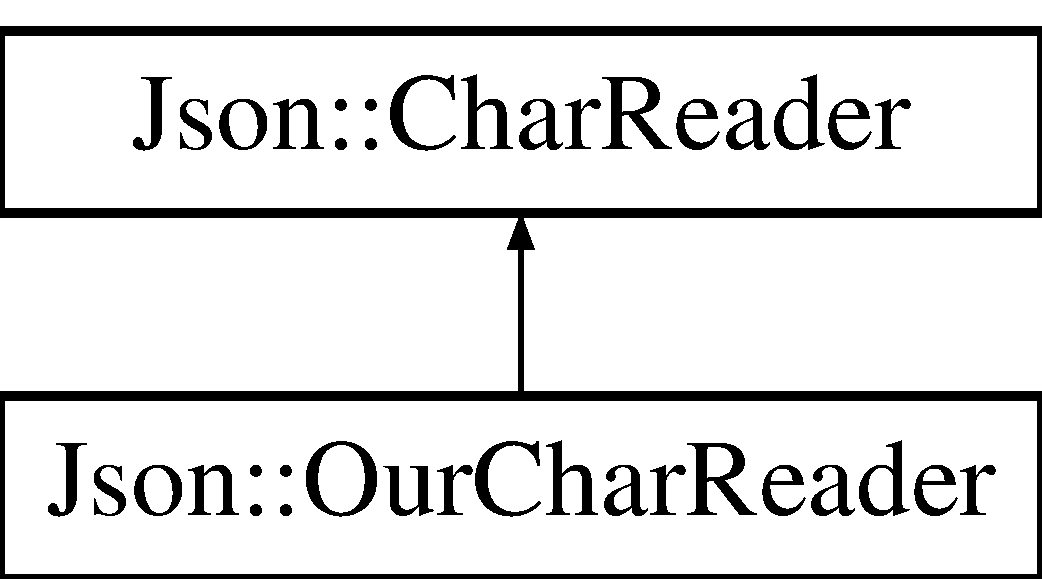
\includegraphics[height=2.000000cm]{classJson_1_1OurCharReader}
\end{center}
\end{figure}
\subsection*{Public Member Functions}
\begin{DoxyCompactItemize}
\item 
\hyperlink{classJson_1_1OurCharReader_a5015506620e7ba7bab417756fa1ca9fe}{Our\+Char\+Reader} (bool collect\+Comments, \hyperlink{classJson_1_1OurFeatures}{Our\+Features} const \&features)
\item 
bool \hyperlink{classJson_1_1OurCharReader_a547f08ec5a9951ca69e8bb2e90296c83}{parse} (char const $\ast$begin\+Doc, char const $\ast$end\+Doc, \hyperlink{classJson_1_1Value}{Value} $\ast$root, \hyperlink{json_8hpp_a1e723f95759de062585bc4a8fd3fa4be}{J\+S\+O\+N\+C\+P\+P\+\_\+\+S\+T\+R\+I\+NG} $\ast$errs) \hyperlink{json_8hpp_a824d6199c91488107e443226fa6022c5}{J\+S\+O\+N\+C\+P\+P\+\_\+\+O\+V\+E\+R\+R\+I\+DE}
\begin{DoxyCompactList}\small\item\em Read a \hyperlink{classJson_1_1Value}{Value} from a \href{http://www.json.org}{\tt J\+S\+ON} document. \end{DoxyCompactList}\end{DoxyCompactItemize}
\subsection*{Private Attributes}
\begin{DoxyCompactItemize}
\item 
bool const \hyperlink{classJson_1_1OurCharReader_aa6afd3d0f754cadad0f6d2be38bcfee0}{collect\+Comments\+\_\+}
\item 
\hyperlink{classJson_1_1OurReader}{Our\+Reader} \hyperlink{classJson_1_1OurCharReader_aedd4520b8570654ed7aa0726075ee58d}{reader\+\_\+}
\end{DoxyCompactItemize}


\subsection{Constructor \& Destructor Documentation}
\index{Json\+::\+Our\+Char\+Reader@{Json\+::\+Our\+Char\+Reader}!Our\+Char\+Reader@{Our\+Char\+Reader}}
\index{Our\+Char\+Reader@{Our\+Char\+Reader}!Json\+::\+Our\+Char\+Reader@{Json\+::\+Our\+Char\+Reader}}
\subsubsection[{\texorpdfstring{Our\+Char\+Reader(bool collect\+Comments, Our\+Features const \&features)}{OurCharReader(bool collectComments, OurFeatures const &features)}}]{\setlength{\rightskip}{0pt plus 5cm}Json\+::\+Our\+Char\+Reader\+::\+Our\+Char\+Reader (
\begin{DoxyParamCaption}
\item[{bool}]{collect\+Comments, }
\item[{{\bf Our\+Features} const \&}]{features}
\end{DoxyParamCaption}
)\hspace{0.3cm}{\ttfamily [inline]}}\hypertarget{classJson_1_1OurCharReader_a5015506620e7ba7bab417756fa1ca9fe}{}\label{classJson_1_1OurCharReader_a5015506620e7ba7bab417756fa1ca9fe}


\subsection{Member Function Documentation}
\index{Json\+::\+Our\+Char\+Reader@{Json\+::\+Our\+Char\+Reader}!parse@{parse}}
\index{parse@{parse}!Json\+::\+Our\+Char\+Reader@{Json\+::\+Our\+Char\+Reader}}
\subsubsection[{\texorpdfstring{parse(char const $\ast$begin\+Doc, char const $\ast$end\+Doc, Value $\ast$root, J\+S\+O\+N\+C\+P\+P\+\_\+\+S\+T\+R\+I\+N\+G $\ast$errs) J\+S\+O\+N\+C\+P\+P\+\_\+\+O\+V\+E\+R\+R\+I\+DE}{parse(char const *beginDoc, char const *endDoc, Value *root, JSONCPP_STRING *errs) JSONCPP_OVERRIDE}}]{\setlength{\rightskip}{0pt plus 5cm}bool Json\+::\+Our\+Char\+Reader\+::parse (
\begin{DoxyParamCaption}
\item[{char const $\ast$}]{begin\+Doc, }
\item[{char const $\ast$}]{end\+Doc, }
\item[{{\bf Value} $\ast$}]{root, }
\item[{{\bf J\+S\+O\+N\+C\+P\+P\+\_\+\+S\+T\+R\+I\+NG} $\ast$}]{errs}
\end{DoxyParamCaption}
)\hspace{0.3cm}{\ttfamily [inline]}, {\ttfamily [virtual]}}\hypertarget{classJson_1_1OurCharReader_a547f08ec5a9951ca69e8bb2e90296c83}{}\label{classJson_1_1OurCharReader_a547f08ec5a9951ca69e8bb2e90296c83}


Read a \hyperlink{classJson_1_1Value}{Value} from a \href{http://www.json.org}{\tt J\+S\+ON} document. 

The document must be a U\+T\+F-\/8 encoded string containing the document to read.


\begin{DoxyParams}{Parameters}
{\em begin\+Doc} & Pointer on the beginning of the U\+T\+F-\/8 encoded string of the document to read. \\
\hline
{\em end\+Doc} & Pointer on the end of the U\+T\+F-\/8 encoded string of the document to read. Must be $>$= begin\+Doc. \\
\hline
{\em root} & \mbox{[}out\mbox{]} Contains the root value of the document if it was successfully parsed. \\
\hline
{\em errs} & \mbox{[}out\mbox{]} Formatted error messages (if not N\+U\+LL) a user friendly string that lists errors in the parsed document. \\
\hline
\end{DoxyParams}
\begin{DoxyReturn}{Returns}
{\ttfamily true} if the document was successfully parsed, {\ttfamily false} if an error occurred. 
\end{DoxyReturn}


Implements \hyperlink{classJson_1_1CharReader_a7983680d50fd0745f371c43b162e78e1}{Json\+::\+Char\+Reader}.



\subsection{Member Data Documentation}
\index{Json\+::\+Our\+Char\+Reader@{Json\+::\+Our\+Char\+Reader}!collect\+Comments\+\_\+@{collect\+Comments\+\_\+}}
\index{collect\+Comments\+\_\+@{collect\+Comments\+\_\+}!Json\+::\+Our\+Char\+Reader@{Json\+::\+Our\+Char\+Reader}}
\subsubsection[{\texorpdfstring{collect\+Comments\+\_\+}{collectComments_}}]{\setlength{\rightskip}{0pt plus 5cm}bool const Json\+::\+Our\+Char\+Reader\+::collect\+Comments\+\_\+\hspace{0.3cm}{\ttfamily [private]}}\hypertarget{classJson_1_1OurCharReader_aa6afd3d0f754cadad0f6d2be38bcfee0}{}\label{classJson_1_1OurCharReader_aa6afd3d0f754cadad0f6d2be38bcfee0}
\index{Json\+::\+Our\+Char\+Reader@{Json\+::\+Our\+Char\+Reader}!reader\+\_\+@{reader\+\_\+}}
\index{reader\+\_\+@{reader\+\_\+}!Json\+::\+Our\+Char\+Reader@{Json\+::\+Our\+Char\+Reader}}
\subsubsection[{\texorpdfstring{reader\+\_\+}{reader_}}]{\setlength{\rightskip}{0pt plus 5cm}{\bf Our\+Reader} Json\+::\+Our\+Char\+Reader\+::reader\+\_\+\hspace{0.3cm}{\ttfamily [private]}}\hypertarget{classJson_1_1OurCharReader_aedd4520b8570654ed7aa0726075ee58d}{}\label{classJson_1_1OurCharReader_aedd4520b8570654ed7aa0726075ee58d}


The documentation for this class was generated from the following file\+:\begin{DoxyCompactItemize}
\item 
/home/pranav/\+Repositories/zcm/src/\hyperlink{json_8cpp}{json.\+cpp}\end{DoxyCompactItemize}

\hypertarget{classJson_1_1OurFeatures}{}\section{Json\+:\+:Our\+Features Class Reference}
\label{classJson_1_1OurFeatures}\index{Json\+::\+Our\+Features@{Json\+::\+Our\+Features}}
\subsection*{Static Public Member Functions}
\begin{DoxyCompactItemize}
\item 
static \hyperlink{classJson_1_1OurFeatures}{Our\+Features} \hyperlink{classJson_1_1OurFeatures_a0686e1406b6677f496529f9f3fe98d1e}{all} ()
\end{DoxyCompactItemize}
\subsection*{Public Attributes}
\begin{DoxyCompactItemize}
\item 
bool \hyperlink{classJson_1_1OurFeatures_ac71bb7ba7363d3b05ed76602b036ce33}{allow\+Comments\+\_\+}
\item 
bool \hyperlink{classJson_1_1OurFeatures_a2095f66a776c0a4ae6cc931a0c94242e}{strict\+Root\+\_\+}
\item 
bool \hyperlink{classJson_1_1OurFeatures_a13963bc44bf948eec1968f7ff8e8f5f1}{allow\+Dropped\+Null\+Placeholders\+\_\+}
\item 
bool \hyperlink{classJson_1_1OurFeatures_af6973fc7e774ce2d634ba99442aeb91a}{allow\+Numeric\+Keys\+\_\+}
\item 
bool \hyperlink{classJson_1_1OurFeatures_abbd6c196d7a22e2a360a59887eda4610}{allow\+Single\+Quotes\+\_\+}
\item 
bool \hyperlink{classJson_1_1OurFeatures_ae8ad25b90706c78f1a8fe929191ac61b}{fail\+If\+Extra\+\_\+}
\item 
bool \hyperlink{classJson_1_1OurFeatures_a39b8e0b86b1c24a45e800c023bb715aa}{reject\+Dup\+Keys\+\_\+}
\item 
bool \hyperlink{classJson_1_1OurFeatures_af760f91cc2a7af37e44f78fb466061bb}{allow\+Special\+Floats\+\_\+}
\item 
int \hyperlink{classJson_1_1OurFeatures_a9a786713902d14be6d57a08cc03ccfff}{stack\+Limit\+\_\+}
\end{DoxyCompactItemize}


\subsection{Member Function Documentation}
\index{Json\+::\+Our\+Features@{Json\+::\+Our\+Features}!all@{all}}
\index{all@{all}!Json\+::\+Our\+Features@{Json\+::\+Our\+Features}}
\subsubsection[{\texorpdfstring{all()}{all()}}]{\setlength{\rightskip}{0pt plus 5cm}{\bf Our\+Features} Json\+::\+Our\+Features\+::all (
\begin{DoxyParamCaption}
{}
\end{DoxyParamCaption}
)\hspace{0.3cm}{\ttfamily [static]}}\hypertarget{classJson_1_1OurFeatures_a0686e1406b6677f496529f9f3fe98d1e}{}\label{classJson_1_1OurFeatures_a0686e1406b6677f496529f9f3fe98d1e}


\subsection{Member Data Documentation}
\index{Json\+::\+Our\+Features@{Json\+::\+Our\+Features}!allow\+Comments\+\_\+@{allow\+Comments\+\_\+}}
\index{allow\+Comments\+\_\+@{allow\+Comments\+\_\+}!Json\+::\+Our\+Features@{Json\+::\+Our\+Features}}
\subsubsection[{\texorpdfstring{allow\+Comments\+\_\+}{allowComments_}}]{\setlength{\rightskip}{0pt plus 5cm}bool Json\+::\+Our\+Features\+::allow\+Comments\+\_\+}\hypertarget{classJson_1_1OurFeatures_ac71bb7ba7363d3b05ed76602b036ce33}{}\label{classJson_1_1OurFeatures_ac71bb7ba7363d3b05ed76602b036ce33}
\index{Json\+::\+Our\+Features@{Json\+::\+Our\+Features}!allow\+Dropped\+Null\+Placeholders\+\_\+@{allow\+Dropped\+Null\+Placeholders\+\_\+}}
\index{allow\+Dropped\+Null\+Placeholders\+\_\+@{allow\+Dropped\+Null\+Placeholders\+\_\+}!Json\+::\+Our\+Features@{Json\+::\+Our\+Features}}
\subsubsection[{\texorpdfstring{allow\+Dropped\+Null\+Placeholders\+\_\+}{allowDroppedNullPlaceholders_}}]{\setlength{\rightskip}{0pt plus 5cm}bool Json\+::\+Our\+Features\+::allow\+Dropped\+Null\+Placeholders\+\_\+}\hypertarget{classJson_1_1OurFeatures_a13963bc44bf948eec1968f7ff8e8f5f1}{}\label{classJson_1_1OurFeatures_a13963bc44bf948eec1968f7ff8e8f5f1}
\index{Json\+::\+Our\+Features@{Json\+::\+Our\+Features}!allow\+Numeric\+Keys\+\_\+@{allow\+Numeric\+Keys\+\_\+}}
\index{allow\+Numeric\+Keys\+\_\+@{allow\+Numeric\+Keys\+\_\+}!Json\+::\+Our\+Features@{Json\+::\+Our\+Features}}
\subsubsection[{\texorpdfstring{allow\+Numeric\+Keys\+\_\+}{allowNumericKeys_}}]{\setlength{\rightskip}{0pt plus 5cm}bool Json\+::\+Our\+Features\+::allow\+Numeric\+Keys\+\_\+}\hypertarget{classJson_1_1OurFeatures_af6973fc7e774ce2d634ba99442aeb91a}{}\label{classJson_1_1OurFeatures_af6973fc7e774ce2d634ba99442aeb91a}
\index{Json\+::\+Our\+Features@{Json\+::\+Our\+Features}!allow\+Single\+Quotes\+\_\+@{allow\+Single\+Quotes\+\_\+}}
\index{allow\+Single\+Quotes\+\_\+@{allow\+Single\+Quotes\+\_\+}!Json\+::\+Our\+Features@{Json\+::\+Our\+Features}}
\subsubsection[{\texorpdfstring{allow\+Single\+Quotes\+\_\+}{allowSingleQuotes_}}]{\setlength{\rightskip}{0pt plus 5cm}bool Json\+::\+Our\+Features\+::allow\+Single\+Quotes\+\_\+}\hypertarget{classJson_1_1OurFeatures_abbd6c196d7a22e2a360a59887eda4610}{}\label{classJson_1_1OurFeatures_abbd6c196d7a22e2a360a59887eda4610}
\index{Json\+::\+Our\+Features@{Json\+::\+Our\+Features}!allow\+Special\+Floats\+\_\+@{allow\+Special\+Floats\+\_\+}}
\index{allow\+Special\+Floats\+\_\+@{allow\+Special\+Floats\+\_\+}!Json\+::\+Our\+Features@{Json\+::\+Our\+Features}}
\subsubsection[{\texorpdfstring{allow\+Special\+Floats\+\_\+}{allowSpecialFloats_}}]{\setlength{\rightskip}{0pt plus 5cm}bool Json\+::\+Our\+Features\+::allow\+Special\+Floats\+\_\+}\hypertarget{classJson_1_1OurFeatures_af760f91cc2a7af37e44f78fb466061bb}{}\label{classJson_1_1OurFeatures_af760f91cc2a7af37e44f78fb466061bb}
\index{Json\+::\+Our\+Features@{Json\+::\+Our\+Features}!fail\+If\+Extra\+\_\+@{fail\+If\+Extra\+\_\+}}
\index{fail\+If\+Extra\+\_\+@{fail\+If\+Extra\+\_\+}!Json\+::\+Our\+Features@{Json\+::\+Our\+Features}}
\subsubsection[{\texorpdfstring{fail\+If\+Extra\+\_\+}{failIfExtra_}}]{\setlength{\rightskip}{0pt plus 5cm}bool Json\+::\+Our\+Features\+::fail\+If\+Extra\+\_\+}\hypertarget{classJson_1_1OurFeatures_ae8ad25b90706c78f1a8fe929191ac61b}{}\label{classJson_1_1OurFeatures_ae8ad25b90706c78f1a8fe929191ac61b}
\index{Json\+::\+Our\+Features@{Json\+::\+Our\+Features}!reject\+Dup\+Keys\+\_\+@{reject\+Dup\+Keys\+\_\+}}
\index{reject\+Dup\+Keys\+\_\+@{reject\+Dup\+Keys\+\_\+}!Json\+::\+Our\+Features@{Json\+::\+Our\+Features}}
\subsubsection[{\texorpdfstring{reject\+Dup\+Keys\+\_\+}{rejectDupKeys_}}]{\setlength{\rightskip}{0pt plus 5cm}bool Json\+::\+Our\+Features\+::reject\+Dup\+Keys\+\_\+}\hypertarget{classJson_1_1OurFeatures_a39b8e0b86b1c24a45e800c023bb715aa}{}\label{classJson_1_1OurFeatures_a39b8e0b86b1c24a45e800c023bb715aa}
\index{Json\+::\+Our\+Features@{Json\+::\+Our\+Features}!stack\+Limit\+\_\+@{stack\+Limit\+\_\+}}
\index{stack\+Limit\+\_\+@{stack\+Limit\+\_\+}!Json\+::\+Our\+Features@{Json\+::\+Our\+Features}}
\subsubsection[{\texorpdfstring{stack\+Limit\+\_\+}{stackLimit_}}]{\setlength{\rightskip}{0pt plus 5cm}int Json\+::\+Our\+Features\+::stack\+Limit\+\_\+}\hypertarget{classJson_1_1OurFeatures_a9a786713902d14be6d57a08cc03ccfff}{}\label{classJson_1_1OurFeatures_a9a786713902d14be6d57a08cc03ccfff}
\index{Json\+::\+Our\+Features@{Json\+::\+Our\+Features}!strict\+Root\+\_\+@{strict\+Root\+\_\+}}
\index{strict\+Root\+\_\+@{strict\+Root\+\_\+}!Json\+::\+Our\+Features@{Json\+::\+Our\+Features}}
\subsubsection[{\texorpdfstring{strict\+Root\+\_\+}{strictRoot_}}]{\setlength{\rightskip}{0pt plus 5cm}bool Json\+::\+Our\+Features\+::strict\+Root\+\_\+}\hypertarget{classJson_1_1OurFeatures_a2095f66a776c0a4ae6cc931a0c94242e}{}\label{classJson_1_1OurFeatures_a2095f66a776c0a4ae6cc931a0c94242e}


The documentation for this class was generated from the following file\+:\begin{DoxyCompactItemize}
\item 
/home/pranav/\+Repositories/zcm/src/\hyperlink{json_8cpp}{json.\+cpp}\end{DoxyCompactItemize}

\hypertarget{classJson_1_1OurReader}{}\section{Json\+:\+:Our\+Reader Class Reference}
\label{classJson_1_1OurReader}\index{Json\+::\+Our\+Reader@{Json\+::\+Our\+Reader}}
\subsection*{Classes}
\begin{DoxyCompactItemize}
\item 
class \hyperlink{classJson_1_1OurReader_1_1ErrorInfo}{Error\+Info}
\item 
struct \hyperlink{structJson_1_1OurReader_1_1StructuredError}{Structured\+Error}
\item 
class \hyperlink{classJson_1_1OurReader_1_1Token}{Token}
\end{DoxyCompactItemize}
\subsection*{Public Types}
\begin{DoxyCompactItemize}
\item 
typedef char \hyperlink{classJson_1_1OurReader_a0cd0bab4caa66594ab843ccd5f9dc239}{Char}
\item 
typedef const \hyperlink{classJson_1_1OurReader_a0cd0bab4caa66594ab843ccd5f9dc239}{Char} $\ast$ \hyperlink{classJson_1_1OurReader_a1bdc7bbc52ba87cae6b19746f2ee0189}{Location}
\end{DoxyCompactItemize}
\subsection*{Public Member Functions}
\begin{DoxyCompactItemize}
\item 
\hyperlink{classJson_1_1OurReader_a48a850914b9c8d7781be172930c478e5}{Our\+Reader} (\hyperlink{classJson_1_1OurFeatures}{Our\+Features} const \&features)
\item 
bool \hyperlink{classJson_1_1OurReader_aba4f8749aab7f02ec17f107e392caf80}{parse} (const char $\ast$begin\+Doc, const char $\ast$end\+Doc, \hyperlink{classJson_1_1Value}{Value} \&root, bool collect\+Comments=true)
\item 
\hyperlink{json_8hpp_a1e723f95759de062585bc4a8fd3fa4be}{J\+S\+O\+N\+C\+P\+P\+\_\+\+S\+T\+R\+I\+NG} \hyperlink{classJson_1_1OurReader_a61b627b274f3bf110d559e4ab50e29b8}{get\+Formatted\+Error\+Messages} () const 
\item 
std\+::vector$<$ \hyperlink{structJson_1_1OurReader_1_1StructuredError}{Structured\+Error} $>$ \hyperlink{classJson_1_1OurReader_a02ef7871af3706754a233c36e6d489e9}{get\+Structured\+Errors} () const 
\item 
bool \hyperlink{classJson_1_1OurReader_a700e9d8e0977fa7e0375d26690d7025f}{push\+Error} (const \hyperlink{classJson_1_1Value}{Value} \&value, const \hyperlink{json_8hpp_a1e723f95759de062585bc4a8fd3fa4be}{J\+S\+O\+N\+C\+P\+P\+\_\+\+S\+T\+R\+I\+NG} \&message)
\item 
bool \hyperlink{classJson_1_1OurReader_addccecfca74b79adaad6115ddd614477}{push\+Error} (const \hyperlink{classJson_1_1Value}{Value} \&value, const \hyperlink{json_8hpp_a1e723f95759de062585bc4a8fd3fa4be}{J\+S\+O\+N\+C\+P\+P\+\_\+\+S\+T\+R\+I\+NG} \&message, const \hyperlink{classJson_1_1Value}{Value} \&extra)
\item 
bool \hyperlink{classJson_1_1OurReader_a048346238d703ad9aed06beb686e6102}{good} () const 
\end{DoxyCompactItemize}
\subsection*{Private Types}
\begin{DoxyCompactItemize}
\item 
enum \hyperlink{classJson_1_1OurReader_a15116f7276ddf1e7a2cc3cbefa884dcc}{Token\+Type} \{ \\*
\hyperlink{classJson_1_1OurReader_a15116f7276ddf1e7a2cc3cbefa884dcca735d1f76eafc2c0c581ed79c077aaa7e}{token\+End\+Of\+Stream} = 0, 
\hyperlink{classJson_1_1OurReader_a15116f7276ddf1e7a2cc3cbefa884dcca7495ef5c356d4faa39b702e528cc7e26}{token\+Object\+Begin}, 
\hyperlink{classJson_1_1OurReader_a15116f7276ddf1e7a2cc3cbefa884dcca8d7e94be97d76ea1c314130b5aabb014}{token\+Object\+End}, 
\hyperlink{classJson_1_1OurReader_a15116f7276ddf1e7a2cc3cbefa884dcca45d229fce2f5f4b52dc0d6c39c853436}{token\+Array\+Begin}, 
\\*
\hyperlink{classJson_1_1OurReader_a15116f7276ddf1e7a2cc3cbefa884dcca59a4f42b50d9731dce6be41818c3d91b}{token\+Array\+End}, 
\hyperlink{classJson_1_1OurReader_a15116f7276ddf1e7a2cc3cbefa884dccadb37e59e1e52cd5e7417bc418b611ce1}{token\+String}, 
\hyperlink{classJson_1_1OurReader_a15116f7276ddf1e7a2cc3cbefa884dcca766aefde855b1246d89b8552240c70d1}{token\+Number}, 
\hyperlink{classJson_1_1OurReader_a15116f7276ddf1e7a2cc3cbefa884dccac7d2a552afcea291d47cf49dfefaf619}{token\+True}, 
\\*
\hyperlink{classJson_1_1OurReader_a15116f7276ddf1e7a2cc3cbefa884dccaab91e3ef98c1cb1326c3674e518c5126}{token\+False}, 
\hyperlink{classJson_1_1OurReader_a15116f7276ddf1e7a2cc3cbefa884dcca4c80b7bb245e3863e38dc8e8586b3c51}{token\+Null}, 
\hyperlink{classJson_1_1OurReader_a15116f7276ddf1e7a2cc3cbefa884dcca167898478691f1ac7a240981ccaa1713}{token\+NaN}, 
\hyperlink{classJson_1_1OurReader_a15116f7276ddf1e7a2cc3cbefa884dcca800c7c7e896d569ebf6c2771eecc7060}{token\+Pos\+Inf}, 
\\*
\hyperlink{classJson_1_1OurReader_a15116f7276ddf1e7a2cc3cbefa884dcca3cf3c4c72d6b5969f17f043a34b2ad4c}{token\+Neg\+Inf}, 
\hyperlink{classJson_1_1OurReader_a15116f7276ddf1e7a2cc3cbefa884dcca8ca62ab9091b149d52ec55828f8040f4}{token\+Array\+Separator}, 
\hyperlink{classJson_1_1OurReader_a15116f7276ddf1e7a2cc3cbefa884dcca7c95881fb1162316bce42c629bf06214}{token\+Member\+Separator}, 
\hyperlink{classJson_1_1OurReader_a15116f7276ddf1e7a2cc3cbefa884dcca777fb6589fdbe225bc10a1e49a090da9}{token\+Comment}, 
\\*
\hyperlink{classJson_1_1OurReader_a15116f7276ddf1e7a2cc3cbefa884dccad39f929b971de8dc55fe84a2d2e3465e}{token\+Error}
 \}
\item 
typedef std\+::deque$<$ \hyperlink{classJson_1_1OurReader_1_1ErrorInfo}{Error\+Info} $>$ \hyperlink{classJson_1_1OurReader_a8cc69593ef7303e58e99bb5dbb767562}{Errors}
\item 
typedef std\+::stack$<$ \hyperlink{classJson_1_1Value}{Value} $\ast$ $>$ \hyperlink{classJson_1_1OurReader_a8480a5ef159cee3a090f96358414d8d3}{Nodes}
\end{DoxyCompactItemize}
\subsection*{Private Member Functions}
\begin{DoxyCompactItemize}
\item 
\hyperlink{classJson_1_1OurReader_aee013005522c0d34d2e14962851487ac}{Our\+Reader} (\hyperlink{classJson_1_1OurReader}{Our\+Reader} const \&)
\item 
void \hyperlink{classJson_1_1OurReader_ad418de7c47bd3d0510888e22110b796e}{operator=} (\hyperlink{classJson_1_1OurReader}{Our\+Reader} const \&)
\item 
bool \hyperlink{classJson_1_1OurReader_a0d1e66da47fe2e85f5033c59326dfdc3}{read\+Token} (\hyperlink{classJson_1_1OurReader_1_1Token}{Token} \&token)
\item 
void \hyperlink{classJson_1_1OurReader_a6fbc6d58a4505e5ccadf330b57b17ca5}{skip\+Spaces} ()
\item 
bool \hyperlink{classJson_1_1OurReader_a4a03f1b266def9b47c4fef35386557fb}{match} (\hyperlink{classJson_1_1OurReader_a1bdc7bbc52ba87cae6b19746f2ee0189}{Location} pattern, int pattern\+Length)
\item 
bool \hyperlink{classJson_1_1OurReader_a90f6bb9e55b2bc3d6c1880809495c222}{read\+Comment} ()
\item 
bool \hyperlink{classJson_1_1OurReader_aba784b125baa1b62387e767b791f2f89}{read\+C\+Style\+Comment} ()
\item 
bool \hyperlink{classJson_1_1OurReader_ae3de80671f0f997053e1c1c8a47a45c5}{read\+Cpp\+Style\+Comment} ()
\item 
bool \hyperlink{classJson_1_1OurReader_a5d39b12671499ec5975f3bbc84b7d438}{read\+String} ()
\item 
bool \hyperlink{classJson_1_1OurReader_ac78592defdc333faf56c6d0908758da3}{read\+String\+Single\+Quote} ()
\item 
bool \hyperlink{classJson_1_1OurReader_aefcb9a78cc45870ccac2db2a66c8ec50}{read\+Number} (bool check\+Inf)
\item 
bool \hyperlink{classJson_1_1OurReader_a1765d9670d191c89a57a22ea5591d35f}{read\+Value} ()
\item 
bool \hyperlink{classJson_1_1OurReader_aea198f8101dba55099f4d8121a993530}{read\+Object} (\hyperlink{classJson_1_1OurReader_1_1Token}{Token} \&token)
\item 
bool \hyperlink{classJson_1_1OurReader_a0b9f58faf4212c6ecb5d8e2a1ac10257}{read\+Array} (\hyperlink{classJson_1_1OurReader_1_1Token}{Token} \&token)
\item 
bool \hyperlink{classJson_1_1OurReader_a272d271290933a89abfd5096dd69c9e9}{decode\+Number} (\hyperlink{classJson_1_1OurReader_1_1Token}{Token} \&token)
\item 
bool \hyperlink{classJson_1_1OurReader_a712270d53a2f023c2f406ac813548340}{decode\+Number} (\hyperlink{classJson_1_1OurReader_1_1Token}{Token} \&token, \hyperlink{classJson_1_1Value}{Value} \&decoded)
\item 
bool \hyperlink{classJson_1_1OurReader_a34e31d8b8399b7ad493359702b6de6c9}{decode\+String} (\hyperlink{classJson_1_1OurReader_1_1Token}{Token} \&token)
\item 
bool \hyperlink{classJson_1_1OurReader_a5046dfa5d43b1770a091aac0a63a9f4b}{decode\+String} (\hyperlink{classJson_1_1OurReader_1_1Token}{Token} \&token, \hyperlink{json_8hpp_a1e723f95759de062585bc4a8fd3fa4be}{J\+S\+O\+N\+C\+P\+P\+\_\+\+S\+T\+R\+I\+NG} \&decoded)
\item 
bool \hyperlink{classJson_1_1OurReader_a1d1c3b44f6720a0e7c39b5ae8de3981c}{decode\+Double} (\hyperlink{classJson_1_1OurReader_1_1Token}{Token} \&token)
\item 
bool \hyperlink{classJson_1_1OurReader_aa5c15a8cd32754f07430dedba3d1308e}{decode\+Double} (\hyperlink{classJson_1_1OurReader_1_1Token}{Token} \&token, \hyperlink{classJson_1_1Value}{Value} \&decoded)
\item 
bool \hyperlink{classJson_1_1OurReader_ac1bf03c161ece082e48da450c50f528d}{decode\+Unicode\+Code\+Point} (\hyperlink{classJson_1_1OurReader_1_1Token}{Token} \&token, \hyperlink{classJson_1_1OurReader_a1bdc7bbc52ba87cae6b19746f2ee0189}{Location} \&current, \hyperlink{classJson_1_1OurReader_a1bdc7bbc52ba87cae6b19746f2ee0189}{Location} end, unsigned int \&unicode)
\item 
bool \hyperlink{classJson_1_1OurReader_adb39be814cc6076b91a0919bdd5b24b0}{decode\+Unicode\+Escape\+Sequence} (\hyperlink{classJson_1_1OurReader_1_1Token}{Token} \&token, \hyperlink{classJson_1_1OurReader_a1bdc7bbc52ba87cae6b19746f2ee0189}{Location} \&current, \hyperlink{classJson_1_1OurReader_a1bdc7bbc52ba87cae6b19746f2ee0189}{Location} end, unsigned int \&unicode)
\item 
bool \hyperlink{classJson_1_1OurReader_aa6a920311e6408ff3a45324d49da18a6}{add\+Error} (const \hyperlink{json_8hpp_a1e723f95759de062585bc4a8fd3fa4be}{J\+S\+O\+N\+C\+P\+P\+\_\+\+S\+T\+R\+I\+NG} \&message, \hyperlink{classJson_1_1OurReader_1_1Token}{Token} \&token, \hyperlink{classJson_1_1OurReader_a1bdc7bbc52ba87cae6b19746f2ee0189}{Location} extra=0)
\item 
bool \hyperlink{classJson_1_1OurReader_a035651f0700a76a815e5f904c63ebb1c}{recover\+From\+Error} (\hyperlink{classJson_1_1OurReader_a15116f7276ddf1e7a2cc3cbefa884dcc}{Token\+Type} skip\+Until\+Token)
\item 
bool \hyperlink{classJson_1_1OurReader_a074cf3d91e9404fe89e03cfc6a43e6fb}{add\+Error\+And\+Recover} (const \hyperlink{json_8hpp_a1e723f95759de062585bc4a8fd3fa4be}{J\+S\+O\+N\+C\+P\+P\+\_\+\+S\+T\+R\+I\+NG} \&message, \hyperlink{classJson_1_1OurReader_1_1Token}{Token} \&token, \hyperlink{classJson_1_1OurReader_a15116f7276ddf1e7a2cc3cbefa884dcc}{Token\+Type} skip\+Until\+Token)
\item 
void \hyperlink{classJson_1_1OurReader_ad48bdaf5b686706f003e792fdbcbf102}{skip\+Until\+Space} ()
\item 
\hyperlink{classJson_1_1Value}{Value} \& \hyperlink{classJson_1_1OurReader_a2acd5b1d53e7d7e17c21ff8e96edc09d}{current\+Value} ()
\item 
\hyperlink{classJson_1_1OurReader_a0cd0bab4caa66594ab843ccd5f9dc239}{Char} \hyperlink{classJson_1_1OurReader_a298285d035fdbc554caae09d9f0a5859}{get\+Next\+Char} ()
\item 
void \hyperlink{classJson_1_1OurReader_a9f47ad324225df1e68bda7dc451845c9}{get\+Location\+Line\+And\+Column} (\hyperlink{classJson_1_1OurReader_a1bdc7bbc52ba87cae6b19746f2ee0189}{Location} location, int \&line, int \&column) const 
\item 
\hyperlink{json_8hpp_a1e723f95759de062585bc4a8fd3fa4be}{J\+S\+O\+N\+C\+P\+P\+\_\+\+S\+T\+R\+I\+NG} \hyperlink{classJson_1_1OurReader_a44fa0d4d376a48bc0b79a99b5b8c5a80}{get\+Location\+Line\+And\+Column} (\hyperlink{classJson_1_1OurReader_a1bdc7bbc52ba87cae6b19746f2ee0189}{Location} location) const 
\item 
void \hyperlink{classJson_1_1OurReader_ad7318c37469a9106069a236fb4b10e1f}{add\+Comment} (\hyperlink{classJson_1_1OurReader_a1bdc7bbc52ba87cae6b19746f2ee0189}{Location} begin, \hyperlink{classJson_1_1OurReader_a1bdc7bbc52ba87cae6b19746f2ee0189}{Location} end, \hyperlink{namespaceJson_a4fc417c23905b2ae9e2c47d197a45351}{Comment\+Placement} placement)
\item 
void \hyperlink{classJson_1_1OurReader_a856dea44d92578c276856d7a65a4ebdc}{skip\+Comment\+Tokens} (\hyperlink{classJson_1_1OurReader_1_1Token}{Token} \&token)
\end{DoxyCompactItemize}
\subsection*{Private Attributes}
\begin{DoxyCompactItemize}
\item 
\hyperlink{classJson_1_1OurReader_a8480a5ef159cee3a090f96358414d8d3}{Nodes} \hyperlink{classJson_1_1OurReader_a19cc4e8c5d17ee6822f752e9a36f4ce3}{nodes\+\_\+}
\item 
\hyperlink{classJson_1_1OurReader_a8cc69593ef7303e58e99bb5dbb767562}{Errors} \hyperlink{classJson_1_1OurReader_afb76b68ba1ab68fe09cf2838e3d4898d}{errors\+\_\+}
\item 
\hyperlink{json_8hpp_a1e723f95759de062585bc4a8fd3fa4be}{J\+S\+O\+N\+C\+P\+P\+\_\+\+S\+T\+R\+I\+NG} \hyperlink{classJson_1_1OurReader_a726230af83d22d25e0c76cec3408ecf1}{document\+\_\+}
\item 
\hyperlink{classJson_1_1OurReader_a1bdc7bbc52ba87cae6b19746f2ee0189}{Location} \hyperlink{classJson_1_1OurReader_a9bda9d72335d52cd06e65f9eca3f70f5}{begin\+\_\+}
\item 
\hyperlink{classJson_1_1OurReader_a1bdc7bbc52ba87cae6b19746f2ee0189}{Location} \hyperlink{classJson_1_1OurReader_ab1f69b0260c27a0d2d65dc56e42c8f9d}{end\+\_\+}
\item 
\hyperlink{classJson_1_1OurReader_a1bdc7bbc52ba87cae6b19746f2ee0189}{Location} \hyperlink{classJson_1_1OurReader_a5211fbbba94be80a22dd2317c621efcc}{current\+\_\+}
\item 
\hyperlink{classJson_1_1OurReader_a1bdc7bbc52ba87cae6b19746f2ee0189}{Location} \hyperlink{classJson_1_1OurReader_a101eadc45e01c60628b53f0db3d13482}{last\+Value\+End\+\_\+}
\item 
\hyperlink{classJson_1_1Value}{Value} $\ast$ \hyperlink{classJson_1_1OurReader_a9f994b6a2227c5d96e6ed6cbc74ed251}{last\+Value\+\_\+}
\item 
\hyperlink{json_8hpp_a1e723f95759de062585bc4a8fd3fa4be}{J\+S\+O\+N\+C\+P\+P\+\_\+\+S\+T\+R\+I\+NG} \hyperlink{classJson_1_1OurReader_a9c53e77e290eb9081298210a955fda6a}{comments\+Before\+\_\+}
\item 
int \hyperlink{classJson_1_1OurReader_aaa91c93bc064c7086248ea01eddcf51a}{stack\+Depth\+\_\+}
\item 
\hyperlink{classJson_1_1OurFeatures}{Our\+Features} const \hyperlink{classJson_1_1OurReader_a2714302d5cc54ca2ce4118ea51c0397a}{features\+\_\+}
\item 
bool \hyperlink{classJson_1_1OurReader_a259f6ac988da2894bcafc670e42f73ad}{collect\+Comments\+\_\+}
\end{DoxyCompactItemize}


\subsection{Member Typedef Documentation}
\index{Json\+::\+Our\+Reader@{Json\+::\+Our\+Reader}!Char@{Char}}
\index{Char@{Char}!Json\+::\+Our\+Reader@{Json\+::\+Our\+Reader}}
\subsubsection[{\texorpdfstring{Char}{Char}}]{\setlength{\rightskip}{0pt plus 5cm}typedef char {\bf Json\+::\+Our\+Reader\+::\+Char}}\hypertarget{classJson_1_1OurReader_a0cd0bab4caa66594ab843ccd5f9dc239}{}\label{classJson_1_1OurReader_a0cd0bab4caa66594ab843ccd5f9dc239}
\index{Json\+::\+Our\+Reader@{Json\+::\+Our\+Reader}!Errors@{Errors}}
\index{Errors@{Errors}!Json\+::\+Our\+Reader@{Json\+::\+Our\+Reader}}
\subsubsection[{\texorpdfstring{Errors}{Errors}}]{\setlength{\rightskip}{0pt plus 5cm}typedef std\+::deque$<${\bf Error\+Info}$>$ {\bf Json\+::\+Our\+Reader\+::\+Errors}\hspace{0.3cm}{\ttfamily [private]}}\hypertarget{classJson_1_1OurReader_a8cc69593ef7303e58e99bb5dbb767562}{}\label{classJson_1_1OurReader_a8cc69593ef7303e58e99bb5dbb767562}
\index{Json\+::\+Our\+Reader@{Json\+::\+Our\+Reader}!Location@{Location}}
\index{Location@{Location}!Json\+::\+Our\+Reader@{Json\+::\+Our\+Reader}}
\subsubsection[{\texorpdfstring{Location}{Location}}]{\setlength{\rightskip}{0pt plus 5cm}typedef const {\bf Char}$\ast$ {\bf Json\+::\+Our\+Reader\+::\+Location}}\hypertarget{classJson_1_1OurReader_a1bdc7bbc52ba87cae6b19746f2ee0189}{}\label{classJson_1_1OurReader_a1bdc7bbc52ba87cae6b19746f2ee0189}
\index{Json\+::\+Our\+Reader@{Json\+::\+Our\+Reader}!Nodes@{Nodes}}
\index{Nodes@{Nodes}!Json\+::\+Our\+Reader@{Json\+::\+Our\+Reader}}
\subsubsection[{\texorpdfstring{Nodes}{Nodes}}]{\setlength{\rightskip}{0pt plus 5cm}typedef std\+::stack$<${\bf Value}$\ast$$>$ {\bf Json\+::\+Our\+Reader\+::\+Nodes}\hspace{0.3cm}{\ttfamily [private]}}\hypertarget{classJson_1_1OurReader_a8480a5ef159cee3a090f96358414d8d3}{}\label{classJson_1_1OurReader_a8480a5ef159cee3a090f96358414d8d3}


\subsection{Member Enumeration Documentation}
\index{Json\+::\+Our\+Reader@{Json\+::\+Our\+Reader}!Token\+Type@{Token\+Type}}
\index{Token\+Type@{Token\+Type}!Json\+::\+Our\+Reader@{Json\+::\+Our\+Reader}}
\subsubsection[{\texorpdfstring{Token\+Type}{TokenType}}]{\setlength{\rightskip}{0pt plus 5cm}enum {\bf Json\+::\+Our\+Reader\+::\+Token\+Type}\hspace{0.3cm}{\ttfamily [private]}}\hypertarget{classJson_1_1OurReader_a15116f7276ddf1e7a2cc3cbefa884dcc}{}\label{classJson_1_1OurReader_a15116f7276ddf1e7a2cc3cbefa884dcc}
\begin{Desc}
\item[Enumerator]\par
\begin{description}
\index{token\+End\+Of\+Stream@{token\+End\+Of\+Stream}!Json\+::\+Our\+Reader@{Json\+::\+Our\+Reader}}\index{Json\+::\+Our\+Reader@{Json\+::\+Our\+Reader}!token\+End\+Of\+Stream@{token\+End\+Of\+Stream}}\item[{\em 
token\+End\+Of\+Stream\hypertarget{classJson_1_1OurReader_a15116f7276ddf1e7a2cc3cbefa884dcca735d1f76eafc2c0c581ed79c077aaa7e}{}\label{classJson_1_1OurReader_a15116f7276ddf1e7a2cc3cbefa884dcca735d1f76eafc2c0c581ed79c077aaa7e}
}]\index{token\+Object\+Begin@{token\+Object\+Begin}!Json\+::\+Our\+Reader@{Json\+::\+Our\+Reader}}\index{Json\+::\+Our\+Reader@{Json\+::\+Our\+Reader}!token\+Object\+Begin@{token\+Object\+Begin}}\item[{\em 
token\+Object\+Begin\hypertarget{classJson_1_1OurReader_a15116f7276ddf1e7a2cc3cbefa884dcca7495ef5c356d4faa39b702e528cc7e26}{}\label{classJson_1_1OurReader_a15116f7276ddf1e7a2cc3cbefa884dcca7495ef5c356d4faa39b702e528cc7e26}
}]\index{token\+Object\+End@{token\+Object\+End}!Json\+::\+Our\+Reader@{Json\+::\+Our\+Reader}}\index{Json\+::\+Our\+Reader@{Json\+::\+Our\+Reader}!token\+Object\+End@{token\+Object\+End}}\item[{\em 
token\+Object\+End\hypertarget{classJson_1_1OurReader_a15116f7276ddf1e7a2cc3cbefa884dcca8d7e94be97d76ea1c314130b5aabb014}{}\label{classJson_1_1OurReader_a15116f7276ddf1e7a2cc3cbefa884dcca8d7e94be97d76ea1c314130b5aabb014}
}]\index{token\+Array\+Begin@{token\+Array\+Begin}!Json\+::\+Our\+Reader@{Json\+::\+Our\+Reader}}\index{Json\+::\+Our\+Reader@{Json\+::\+Our\+Reader}!token\+Array\+Begin@{token\+Array\+Begin}}\item[{\em 
token\+Array\+Begin\hypertarget{classJson_1_1OurReader_a15116f7276ddf1e7a2cc3cbefa884dcca45d229fce2f5f4b52dc0d6c39c853436}{}\label{classJson_1_1OurReader_a15116f7276ddf1e7a2cc3cbefa884dcca45d229fce2f5f4b52dc0d6c39c853436}
}]\index{token\+Array\+End@{token\+Array\+End}!Json\+::\+Our\+Reader@{Json\+::\+Our\+Reader}}\index{Json\+::\+Our\+Reader@{Json\+::\+Our\+Reader}!token\+Array\+End@{token\+Array\+End}}\item[{\em 
token\+Array\+End\hypertarget{classJson_1_1OurReader_a15116f7276ddf1e7a2cc3cbefa884dcca59a4f42b50d9731dce6be41818c3d91b}{}\label{classJson_1_1OurReader_a15116f7276ddf1e7a2cc3cbefa884dcca59a4f42b50d9731dce6be41818c3d91b}
}]\index{token\+String@{token\+String}!Json\+::\+Our\+Reader@{Json\+::\+Our\+Reader}}\index{Json\+::\+Our\+Reader@{Json\+::\+Our\+Reader}!token\+String@{token\+String}}\item[{\em 
token\+String\hypertarget{classJson_1_1OurReader_a15116f7276ddf1e7a2cc3cbefa884dccadb37e59e1e52cd5e7417bc418b611ce1}{}\label{classJson_1_1OurReader_a15116f7276ddf1e7a2cc3cbefa884dccadb37e59e1e52cd5e7417bc418b611ce1}
}]\index{token\+Number@{token\+Number}!Json\+::\+Our\+Reader@{Json\+::\+Our\+Reader}}\index{Json\+::\+Our\+Reader@{Json\+::\+Our\+Reader}!token\+Number@{token\+Number}}\item[{\em 
token\+Number\hypertarget{classJson_1_1OurReader_a15116f7276ddf1e7a2cc3cbefa884dcca766aefde855b1246d89b8552240c70d1}{}\label{classJson_1_1OurReader_a15116f7276ddf1e7a2cc3cbefa884dcca766aefde855b1246d89b8552240c70d1}
}]\index{token\+True@{token\+True}!Json\+::\+Our\+Reader@{Json\+::\+Our\+Reader}}\index{Json\+::\+Our\+Reader@{Json\+::\+Our\+Reader}!token\+True@{token\+True}}\item[{\em 
token\+True\hypertarget{classJson_1_1OurReader_a15116f7276ddf1e7a2cc3cbefa884dccac7d2a552afcea291d47cf49dfefaf619}{}\label{classJson_1_1OurReader_a15116f7276ddf1e7a2cc3cbefa884dccac7d2a552afcea291d47cf49dfefaf619}
}]\index{token\+False@{token\+False}!Json\+::\+Our\+Reader@{Json\+::\+Our\+Reader}}\index{Json\+::\+Our\+Reader@{Json\+::\+Our\+Reader}!token\+False@{token\+False}}\item[{\em 
token\+False\hypertarget{classJson_1_1OurReader_a15116f7276ddf1e7a2cc3cbefa884dccaab91e3ef98c1cb1326c3674e518c5126}{}\label{classJson_1_1OurReader_a15116f7276ddf1e7a2cc3cbefa884dccaab91e3ef98c1cb1326c3674e518c5126}
}]\index{token\+Null@{token\+Null}!Json\+::\+Our\+Reader@{Json\+::\+Our\+Reader}}\index{Json\+::\+Our\+Reader@{Json\+::\+Our\+Reader}!token\+Null@{token\+Null}}\item[{\em 
token\+Null\hypertarget{classJson_1_1OurReader_a15116f7276ddf1e7a2cc3cbefa884dcca4c80b7bb245e3863e38dc8e8586b3c51}{}\label{classJson_1_1OurReader_a15116f7276ddf1e7a2cc3cbefa884dcca4c80b7bb245e3863e38dc8e8586b3c51}
}]\index{token\+NaN@{token\+NaN}!Json\+::\+Our\+Reader@{Json\+::\+Our\+Reader}}\index{Json\+::\+Our\+Reader@{Json\+::\+Our\+Reader}!token\+NaN@{token\+NaN}}\item[{\em 
token\+NaN\hypertarget{classJson_1_1OurReader_a15116f7276ddf1e7a2cc3cbefa884dcca167898478691f1ac7a240981ccaa1713}{}\label{classJson_1_1OurReader_a15116f7276ddf1e7a2cc3cbefa884dcca167898478691f1ac7a240981ccaa1713}
}]\index{token\+Pos\+Inf@{token\+Pos\+Inf}!Json\+::\+Our\+Reader@{Json\+::\+Our\+Reader}}\index{Json\+::\+Our\+Reader@{Json\+::\+Our\+Reader}!token\+Pos\+Inf@{token\+Pos\+Inf}}\item[{\em 
token\+Pos\+Inf\hypertarget{classJson_1_1OurReader_a15116f7276ddf1e7a2cc3cbefa884dcca800c7c7e896d569ebf6c2771eecc7060}{}\label{classJson_1_1OurReader_a15116f7276ddf1e7a2cc3cbefa884dcca800c7c7e896d569ebf6c2771eecc7060}
}]\index{token\+Neg\+Inf@{token\+Neg\+Inf}!Json\+::\+Our\+Reader@{Json\+::\+Our\+Reader}}\index{Json\+::\+Our\+Reader@{Json\+::\+Our\+Reader}!token\+Neg\+Inf@{token\+Neg\+Inf}}\item[{\em 
token\+Neg\+Inf\hypertarget{classJson_1_1OurReader_a15116f7276ddf1e7a2cc3cbefa884dcca3cf3c4c72d6b5969f17f043a34b2ad4c}{}\label{classJson_1_1OurReader_a15116f7276ddf1e7a2cc3cbefa884dcca3cf3c4c72d6b5969f17f043a34b2ad4c}
}]\index{token\+Array\+Separator@{token\+Array\+Separator}!Json\+::\+Our\+Reader@{Json\+::\+Our\+Reader}}\index{Json\+::\+Our\+Reader@{Json\+::\+Our\+Reader}!token\+Array\+Separator@{token\+Array\+Separator}}\item[{\em 
token\+Array\+Separator\hypertarget{classJson_1_1OurReader_a15116f7276ddf1e7a2cc3cbefa884dcca8ca62ab9091b149d52ec55828f8040f4}{}\label{classJson_1_1OurReader_a15116f7276ddf1e7a2cc3cbefa884dcca8ca62ab9091b149d52ec55828f8040f4}
}]\index{token\+Member\+Separator@{token\+Member\+Separator}!Json\+::\+Our\+Reader@{Json\+::\+Our\+Reader}}\index{Json\+::\+Our\+Reader@{Json\+::\+Our\+Reader}!token\+Member\+Separator@{token\+Member\+Separator}}\item[{\em 
token\+Member\+Separator\hypertarget{classJson_1_1OurReader_a15116f7276ddf1e7a2cc3cbefa884dcca7c95881fb1162316bce42c629bf06214}{}\label{classJson_1_1OurReader_a15116f7276ddf1e7a2cc3cbefa884dcca7c95881fb1162316bce42c629bf06214}
}]\index{token\+Comment@{token\+Comment}!Json\+::\+Our\+Reader@{Json\+::\+Our\+Reader}}\index{Json\+::\+Our\+Reader@{Json\+::\+Our\+Reader}!token\+Comment@{token\+Comment}}\item[{\em 
token\+Comment\hypertarget{classJson_1_1OurReader_a15116f7276ddf1e7a2cc3cbefa884dcca777fb6589fdbe225bc10a1e49a090da9}{}\label{classJson_1_1OurReader_a15116f7276ddf1e7a2cc3cbefa884dcca777fb6589fdbe225bc10a1e49a090da9}
}]\index{token\+Error@{token\+Error}!Json\+::\+Our\+Reader@{Json\+::\+Our\+Reader}}\index{Json\+::\+Our\+Reader@{Json\+::\+Our\+Reader}!token\+Error@{token\+Error}}\item[{\em 
token\+Error\hypertarget{classJson_1_1OurReader_a15116f7276ddf1e7a2cc3cbefa884dccad39f929b971de8dc55fe84a2d2e3465e}{}\label{classJson_1_1OurReader_a15116f7276ddf1e7a2cc3cbefa884dccad39f929b971de8dc55fe84a2d2e3465e}
}]\end{description}
\end{Desc}


\subsection{Constructor \& Destructor Documentation}
\index{Json\+::\+Our\+Reader@{Json\+::\+Our\+Reader}!Our\+Reader@{Our\+Reader}}
\index{Our\+Reader@{Our\+Reader}!Json\+::\+Our\+Reader@{Json\+::\+Our\+Reader}}
\subsubsection[{\texorpdfstring{Our\+Reader(\+Our\+Features const \&features)}{OurReader(OurFeatures const &features)}}]{\setlength{\rightskip}{0pt plus 5cm}Json\+::\+Our\+Reader\+::\+Our\+Reader (
\begin{DoxyParamCaption}
\item[{{\bf Our\+Features} const \&}]{features}
\end{DoxyParamCaption}
)}\hypertarget{classJson_1_1OurReader_a48a850914b9c8d7781be172930c478e5}{}\label{classJson_1_1OurReader_a48a850914b9c8d7781be172930c478e5}
\index{Json\+::\+Our\+Reader@{Json\+::\+Our\+Reader}!Our\+Reader@{Our\+Reader}}
\index{Our\+Reader@{Our\+Reader}!Json\+::\+Our\+Reader@{Json\+::\+Our\+Reader}}
\subsubsection[{\texorpdfstring{Our\+Reader(\+Our\+Reader const \&)}{OurReader(OurReader const &)}}]{\setlength{\rightskip}{0pt plus 5cm}Json\+::\+Our\+Reader\+::\+Our\+Reader (
\begin{DoxyParamCaption}
\item[{{\bf Our\+Reader} const \&}]{}
\end{DoxyParamCaption}
)\hspace{0.3cm}{\ttfamily [private]}}\hypertarget{classJson_1_1OurReader_aee013005522c0d34d2e14962851487ac}{}\label{classJson_1_1OurReader_aee013005522c0d34d2e14962851487ac}


\subsection{Member Function Documentation}
\index{Json\+::\+Our\+Reader@{Json\+::\+Our\+Reader}!add\+Comment@{add\+Comment}}
\index{add\+Comment@{add\+Comment}!Json\+::\+Our\+Reader@{Json\+::\+Our\+Reader}}
\subsubsection[{\texorpdfstring{add\+Comment(\+Location begin, Location end, Comment\+Placement placement)}{addComment(Location begin, Location end, CommentPlacement placement)}}]{\setlength{\rightskip}{0pt plus 5cm}void Json\+::\+Our\+Reader\+::add\+Comment (
\begin{DoxyParamCaption}
\item[{{\bf Location}}]{begin, }
\item[{{\bf Location}}]{end, }
\item[{{\bf Comment\+Placement}}]{placement}
\end{DoxyParamCaption}
)\hspace{0.3cm}{\ttfamily [private]}}\hypertarget{classJson_1_1OurReader_ad7318c37469a9106069a236fb4b10e1f}{}\label{classJson_1_1OurReader_ad7318c37469a9106069a236fb4b10e1f}
\index{Json\+::\+Our\+Reader@{Json\+::\+Our\+Reader}!add\+Error@{add\+Error}}
\index{add\+Error@{add\+Error}!Json\+::\+Our\+Reader@{Json\+::\+Our\+Reader}}
\subsubsection[{\texorpdfstring{add\+Error(const J\+S\+O\+N\+C\+P\+P\+\_\+\+S\+T\+R\+I\+N\+G \&message, Token \&token, Location extra=0)}{addError(const JSONCPP_STRING &message, Token &token, Location extra=0)}}]{\setlength{\rightskip}{0pt plus 5cm}bool Json\+::\+Our\+Reader\+::add\+Error (
\begin{DoxyParamCaption}
\item[{const {\bf J\+S\+O\+N\+C\+P\+P\+\_\+\+S\+T\+R\+I\+NG} \&}]{message, }
\item[{{\bf Token} \&}]{token, }
\item[{{\bf Location}}]{extra = {\ttfamily 0}}
\end{DoxyParamCaption}
)\hspace{0.3cm}{\ttfamily [private]}}\hypertarget{classJson_1_1OurReader_aa6a920311e6408ff3a45324d49da18a6}{}\label{classJson_1_1OurReader_aa6a920311e6408ff3a45324d49da18a6}
\index{Json\+::\+Our\+Reader@{Json\+::\+Our\+Reader}!add\+Error\+And\+Recover@{add\+Error\+And\+Recover}}
\index{add\+Error\+And\+Recover@{add\+Error\+And\+Recover}!Json\+::\+Our\+Reader@{Json\+::\+Our\+Reader}}
\subsubsection[{\texorpdfstring{add\+Error\+And\+Recover(const J\+S\+O\+N\+C\+P\+P\+\_\+\+S\+T\+R\+I\+N\+G \&message, Token \&token, Token\+Type skip\+Until\+Token)}{addErrorAndRecover(const JSONCPP_STRING &message, Token &token, TokenType skipUntilToken)}}]{\setlength{\rightskip}{0pt plus 5cm}bool Json\+::\+Our\+Reader\+::add\+Error\+And\+Recover (
\begin{DoxyParamCaption}
\item[{const {\bf J\+S\+O\+N\+C\+P\+P\+\_\+\+S\+T\+R\+I\+NG} \&}]{message, }
\item[{{\bf Token} \&}]{token, }
\item[{{\bf Token\+Type}}]{skip\+Until\+Token}
\end{DoxyParamCaption}
)\hspace{0.3cm}{\ttfamily [private]}}\hypertarget{classJson_1_1OurReader_a074cf3d91e9404fe89e03cfc6a43e6fb}{}\label{classJson_1_1OurReader_a074cf3d91e9404fe89e03cfc6a43e6fb}
\index{Json\+::\+Our\+Reader@{Json\+::\+Our\+Reader}!current\+Value@{current\+Value}}
\index{current\+Value@{current\+Value}!Json\+::\+Our\+Reader@{Json\+::\+Our\+Reader}}
\subsubsection[{\texorpdfstring{current\+Value()}{currentValue()}}]{\setlength{\rightskip}{0pt plus 5cm}{\bf Value} \& Json\+::\+Our\+Reader\+::current\+Value (
\begin{DoxyParamCaption}
{}
\end{DoxyParamCaption}
)\hspace{0.3cm}{\ttfamily [private]}}\hypertarget{classJson_1_1OurReader_a2acd5b1d53e7d7e17c21ff8e96edc09d}{}\label{classJson_1_1OurReader_a2acd5b1d53e7d7e17c21ff8e96edc09d}
\index{Json\+::\+Our\+Reader@{Json\+::\+Our\+Reader}!decode\+Double@{decode\+Double}}
\index{decode\+Double@{decode\+Double}!Json\+::\+Our\+Reader@{Json\+::\+Our\+Reader}}
\subsubsection[{\texorpdfstring{decode\+Double(\+Token \&token)}{decodeDouble(Token &token)}}]{\setlength{\rightskip}{0pt plus 5cm}bool Json\+::\+Our\+Reader\+::decode\+Double (
\begin{DoxyParamCaption}
\item[{{\bf Token} \&}]{token}
\end{DoxyParamCaption}
)\hspace{0.3cm}{\ttfamily [private]}}\hypertarget{classJson_1_1OurReader_a1d1c3b44f6720a0e7c39b5ae8de3981c}{}\label{classJson_1_1OurReader_a1d1c3b44f6720a0e7c39b5ae8de3981c}
\index{Json\+::\+Our\+Reader@{Json\+::\+Our\+Reader}!decode\+Double@{decode\+Double}}
\index{decode\+Double@{decode\+Double}!Json\+::\+Our\+Reader@{Json\+::\+Our\+Reader}}
\subsubsection[{\texorpdfstring{decode\+Double(\+Token \&token, Value \&decoded)}{decodeDouble(Token &token, Value &decoded)}}]{\setlength{\rightskip}{0pt plus 5cm}bool Json\+::\+Our\+Reader\+::decode\+Double (
\begin{DoxyParamCaption}
\item[{{\bf Token} \&}]{token, }
\item[{{\bf Value} \&}]{decoded}
\end{DoxyParamCaption}
)\hspace{0.3cm}{\ttfamily [private]}}\hypertarget{classJson_1_1OurReader_aa5c15a8cd32754f07430dedba3d1308e}{}\label{classJson_1_1OurReader_aa5c15a8cd32754f07430dedba3d1308e}
\index{Json\+::\+Our\+Reader@{Json\+::\+Our\+Reader}!decode\+Number@{decode\+Number}}
\index{decode\+Number@{decode\+Number}!Json\+::\+Our\+Reader@{Json\+::\+Our\+Reader}}
\subsubsection[{\texorpdfstring{decode\+Number(\+Token \&token)}{decodeNumber(Token &token)}}]{\setlength{\rightskip}{0pt plus 5cm}bool Json\+::\+Our\+Reader\+::decode\+Number (
\begin{DoxyParamCaption}
\item[{{\bf Token} \&}]{token}
\end{DoxyParamCaption}
)\hspace{0.3cm}{\ttfamily [private]}}\hypertarget{classJson_1_1OurReader_a272d271290933a89abfd5096dd69c9e9}{}\label{classJson_1_1OurReader_a272d271290933a89abfd5096dd69c9e9}
\index{Json\+::\+Our\+Reader@{Json\+::\+Our\+Reader}!decode\+Number@{decode\+Number}}
\index{decode\+Number@{decode\+Number}!Json\+::\+Our\+Reader@{Json\+::\+Our\+Reader}}
\subsubsection[{\texorpdfstring{decode\+Number(\+Token \&token, Value \&decoded)}{decodeNumber(Token &token, Value &decoded)}}]{\setlength{\rightskip}{0pt plus 5cm}bool Json\+::\+Our\+Reader\+::decode\+Number (
\begin{DoxyParamCaption}
\item[{{\bf Token} \&}]{token, }
\item[{{\bf Value} \&}]{decoded}
\end{DoxyParamCaption}
)\hspace{0.3cm}{\ttfamily [private]}}\hypertarget{classJson_1_1OurReader_a712270d53a2f023c2f406ac813548340}{}\label{classJson_1_1OurReader_a712270d53a2f023c2f406ac813548340}
\index{Json\+::\+Our\+Reader@{Json\+::\+Our\+Reader}!decode\+String@{decode\+String}}
\index{decode\+String@{decode\+String}!Json\+::\+Our\+Reader@{Json\+::\+Our\+Reader}}
\subsubsection[{\texorpdfstring{decode\+String(\+Token \&token)}{decodeString(Token &token)}}]{\setlength{\rightskip}{0pt plus 5cm}bool Json\+::\+Our\+Reader\+::decode\+String (
\begin{DoxyParamCaption}
\item[{{\bf Token} \&}]{token}
\end{DoxyParamCaption}
)\hspace{0.3cm}{\ttfamily [private]}}\hypertarget{classJson_1_1OurReader_a34e31d8b8399b7ad493359702b6de6c9}{}\label{classJson_1_1OurReader_a34e31d8b8399b7ad493359702b6de6c9}
\index{Json\+::\+Our\+Reader@{Json\+::\+Our\+Reader}!decode\+String@{decode\+String}}
\index{decode\+String@{decode\+String}!Json\+::\+Our\+Reader@{Json\+::\+Our\+Reader}}
\subsubsection[{\texorpdfstring{decode\+String(\+Token \&token, J\+S\+O\+N\+C\+P\+P\+\_\+\+S\+T\+R\+I\+N\+G \&decoded)}{decodeString(Token &token, JSONCPP_STRING &decoded)}}]{\setlength{\rightskip}{0pt plus 5cm}bool Json\+::\+Our\+Reader\+::decode\+String (
\begin{DoxyParamCaption}
\item[{{\bf Token} \&}]{token, }
\item[{{\bf J\+S\+O\+N\+C\+P\+P\+\_\+\+S\+T\+R\+I\+NG} \&}]{decoded}
\end{DoxyParamCaption}
)\hspace{0.3cm}{\ttfamily [private]}}\hypertarget{classJson_1_1OurReader_a5046dfa5d43b1770a091aac0a63a9f4b}{}\label{classJson_1_1OurReader_a5046dfa5d43b1770a091aac0a63a9f4b}
\index{Json\+::\+Our\+Reader@{Json\+::\+Our\+Reader}!decode\+Unicode\+Code\+Point@{decode\+Unicode\+Code\+Point}}
\index{decode\+Unicode\+Code\+Point@{decode\+Unicode\+Code\+Point}!Json\+::\+Our\+Reader@{Json\+::\+Our\+Reader}}
\subsubsection[{\texorpdfstring{decode\+Unicode\+Code\+Point(\+Token \&token, Location \&current, Location end, unsigned int \&unicode)}{decodeUnicodeCodePoint(Token &token, Location &current, Location end, unsigned int &unicode)}}]{\setlength{\rightskip}{0pt plus 5cm}bool Json\+::\+Our\+Reader\+::decode\+Unicode\+Code\+Point (
\begin{DoxyParamCaption}
\item[{{\bf Token} \&}]{token, }
\item[{{\bf Location} \&}]{current, }
\item[{{\bf Location}}]{end, }
\item[{unsigned int \&}]{unicode}
\end{DoxyParamCaption}
)\hspace{0.3cm}{\ttfamily [private]}}\hypertarget{classJson_1_1OurReader_ac1bf03c161ece082e48da450c50f528d}{}\label{classJson_1_1OurReader_ac1bf03c161ece082e48da450c50f528d}
\index{Json\+::\+Our\+Reader@{Json\+::\+Our\+Reader}!decode\+Unicode\+Escape\+Sequence@{decode\+Unicode\+Escape\+Sequence}}
\index{decode\+Unicode\+Escape\+Sequence@{decode\+Unicode\+Escape\+Sequence}!Json\+::\+Our\+Reader@{Json\+::\+Our\+Reader}}
\subsubsection[{\texorpdfstring{decode\+Unicode\+Escape\+Sequence(\+Token \&token, Location \&current, Location end, unsigned int \&unicode)}{decodeUnicodeEscapeSequence(Token &token, Location &current, Location end, unsigned int &unicode)}}]{\setlength{\rightskip}{0pt plus 5cm}bool Json\+::\+Our\+Reader\+::decode\+Unicode\+Escape\+Sequence (
\begin{DoxyParamCaption}
\item[{{\bf Token} \&}]{token, }
\item[{{\bf Location} \&}]{current, }
\item[{{\bf Location}}]{end, }
\item[{unsigned int \&}]{unicode}
\end{DoxyParamCaption}
)\hspace{0.3cm}{\ttfamily [private]}}\hypertarget{classJson_1_1OurReader_adb39be814cc6076b91a0919bdd5b24b0}{}\label{classJson_1_1OurReader_adb39be814cc6076b91a0919bdd5b24b0}
\index{Json\+::\+Our\+Reader@{Json\+::\+Our\+Reader}!get\+Formatted\+Error\+Messages@{get\+Formatted\+Error\+Messages}}
\index{get\+Formatted\+Error\+Messages@{get\+Formatted\+Error\+Messages}!Json\+::\+Our\+Reader@{Json\+::\+Our\+Reader}}
\subsubsection[{\texorpdfstring{get\+Formatted\+Error\+Messages() const }{getFormattedErrorMessages() const }}]{\setlength{\rightskip}{0pt plus 5cm}{\bf J\+S\+O\+N\+C\+P\+P\+\_\+\+S\+T\+R\+I\+NG} Json\+::\+Our\+Reader\+::get\+Formatted\+Error\+Messages (
\begin{DoxyParamCaption}
{}
\end{DoxyParamCaption}
) const}\hypertarget{classJson_1_1OurReader_a61b627b274f3bf110d559e4ab50e29b8}{}\label{classJson_1_1OurReader_a61b627b274f3bf110d559e4ab50e29b8}
\index{Json\+::\+Our\+Reader@{Json\+::\+Our\+Reader}!get\+Location\+Line\+And\+Column@{get\+Location\+Line\+And\+Column}}
\index{get\+Location\+Line\+And\+Column@{get\+Location\+Line\+And\+Column}!Json\+::\+Our\+Reader@{Json\+::\+Our\+Reader}}
\subsubsection[{\texorpdfstring{get\+Location\+Line\+And\+Column(\+Location location, int \&line, int \&column) const }{getLocationLineAndColumn(Location location, int &line, int &column) const }}]{\setlength{\rightskip}{0pt plus 5cm}void Json\+::\+Our\+Reader\+::get\+Location\+Line\+And\+Column (
\begin{DoxyParamCaption}
\item[{{\bf Location}}]{location, }
\item[{int \&}]{line, }
\item[{int \&}]{column}
\end{DoxyParamCaption}
) const\hspace{0.3cm}{\ttfamily [private]}}\hypertarget{classJson_1_1OurReader_a9f47ad324225df1e68bda7dc451845c9}{}\label{classJson_1_1OurReader_a9f47ad324225df1e68bda7dc451845c9}
\index{Json\+::\+Our\+Reader@{Json\+::\+Our\+Reader}!get\+Location\+Line\+And\+Column@{get\+Location\+Line\+And\+Column}}
\index{get\+Location\+Line\+And\+Column@{get\+Location\+Line\+And\+Column}!Json\+::\+Our\+Reader@{Json\+::\+Our\+Reader}}
\subsubsection[{\texorpdfstring{get\+Location\+Line\+And\+Column(\+Location location) const }{getLocationLineAndColumn(Location location) const }}]{\setlength{\rightskip}{0pt plus 5cm}{\bf J\+S\+O\+N\+C\+P\+P\+\_\+\+S\+T\+R\+I\+NG} Json\+::\+Our\+Reader\+::get\+Location\+Line\+And\+Column (
\begin{DoxyParamCaption}
\item[{{\bf Location}}]{location}
\end{DoxyParamCaption}
) const\hspace{0.3cm}{\ttfamily [private]}}\hypertarget{classJson_1_1OurReader_a44fa0d4d376a48bc0b79a99b5b8c5a80}{}\label{classJson_1_1OurReader_a44fa0d4d376a48bc0b79a99b5b8c5a80}
\index{Json\+::\+Our\+Reader@{Json\+::\+Our\+Reader}!get\+Next\+Char@{get\+Next\+Char}}
\index{get\+Next\+Char@{get\+Next\+Char}!Json\+::\+Our\+Reader@{Json\+::\+Our\+Reader}}
\subsubsection[{\texorpdfstring{get\+Next\+Char()}{getNextChar()}}]{\setlength{\rightskip}{0pt plus 5cm}{\bf Our\+Reader\+::\+Char} Json\+::\+Our\+Reader\+::get\+Next\+Char (
\begin{DoxyParamCaption}
{}
\end{DoxyParamCaption}
)\hspace{0.3cm}{\ttfamily [private]}}\hypertarget{classJson_1_1OurReader_a298285d035fdbc554caae09d9f0a5859}{}\label{classJson_1_1OurReader_a298285d035fdbc554caae09d9f0a5859}
\index{Json\+::\+Our\+Reader@{Json\+::\+Our\+Reader}!get\+Structured\+Errors@{get\+Structured\+Errors}}
\index{get\+Structured\+Errors@{get\+Structured\+Errors}!Json\+::\+Our\+Reader@{Json\+::\+Our\+Reader}}
\subsubsection[{\texorpdfstring{get\+Structured\+Errors() const }{getStructuredErrors() const }}]{\setlength{\rightskip}{0pt plus 5cm}std\+::vector$<$ {\bf Our\+Reader\+::\+Structured\+Error} $>$ Json\+::\+Our\+Reader\+::get\+Structured\+Errors (
\begin{DoxyParamCaption}
{}
\end{DoxyParamCaption}
) const}\hypertarget{classJson_1_1OurReader_a02ef7871af3706754a233c36e6d489e9}{}\label{classJson_1_1OurReader_a02ef7871af3706754a233c36e6d489e9}
\index{Json\+::\+Our\+Reader@{Json\+::\+Our\+Reader}!good@{good}}
\index{good@{good}!Json\+::\+Our\+Reader@{Json\+::\+Our\+Reader}}
\subsubsection[{\texorpdfstring{good() const }{good() const }}]{\setlength{\rightskip}{0pt plus 5cm}bool Json\+::\+Our\+Reader\+::good (
\begin{DoxyParamCaption}
{}
\end{DoxyParamCaption}
) const}\hypertarget{classJson_1_1OurReader_a048346238d703ad9aed06beb686e6102}{}\label{classJson_1_1OurReader_a048346238d703ad9aed06beb686e6102}
\index{Json\+::\+Our\+Reader@{Json\+::\+Our\+Reader}!match@{match}}
\index{match@{match}!Json\+::\+Our\+Reader@{Json\+::\+Our\+Reader}}
\subsubsection[{\texorpdfstring{match(\+Location pattern, int pattern\+Length)}{match(Location pattern, int patternLength)}}]{\setlength{\rightskip}{0pt plus 5cm}bool Json\+::\+Our\+Reader\+::match (
\begin{DoxyParamCaption}
\item[{{\bf Location}}]{pattern, }
\item[{int}]{pattern\+Length}
\end{DoxyParamCaption}
)\hspace{0.3cm}{\ttfamily [private]}}\hypertarget{classJson_1_1OurReader_a4a03f1b266def9b47c4fef35386557fb}{}\label{classJson_1_1OurReader_a4a03f1b266def9b47c4fef35386557fb}
\index{Json\+::\+Our\+Reader@{Json\+::\+Our\+Reader}!operator=@{operator=}}
\index{operator=@{operator=}!Json\+::\+Our\+Reader@{Json\+::\+Our\+Reader}}
\subsubsection[{\texorpdfstring{operator=(\+Our\+Reader const \&)}{operator=(OurReader const &)}}]{\setlength{\rightskip}{0pt plus 5cm}void Json\+::\+Our\+Reader\+::operator= (
\begin{DoxyParamCaption}
\item[{{\bf Our\+Reader} const \&}]{}
\end{DoxyParamCaption}
)\hspace{0.3cm}{\ttfamily [private]}}\hypertarget{classJson_1_1OurReader_ad418de7c47bd3d0510888e22110b796e}{}\label{classJson_1_1OurReader_ad418de7c47bd3d0510888e22110b796e}
\index{Json\+::\+Our\+Reader@{Json\+::\+Our\+Reader}!parse@{parse}}
\index{parse@{parse}!Json\+::\+Our\+Reader@{Json\+::\+Our\+Reader}}
\subsubsection[{\texorpdfstring{parse(const char $\ast$begin\+Doc, const char $\ast$end\+Doc, Value \&root, bool collect\+Comments=true)}{parse(const char *beginDoc, const char *endDoc, Value &root, bool collectComments=true)}}]{\setlength{\rightskip}{0pt plus 5cm}bool Json\+::\+Our\+Reader\+::parse (
\begin{DoxyParamCaption}
\item[{const char $\ast$}]{begin\+Doc, }
\item[{const char $\ast$}]{end\+Doc, }
\item[{{\bf Value} \&}]{root, }
\item[{bool}]{collect\+Comments = {\ttfamily true}}
\end{DoxyParamCaption}
)}\hypertarget{classJson_1_1OurReader_aba4f8749aab7f02ec17f107e392caf80}{}\label{classJson_1_1OurReader_aba4f8749aab7f02ec17f107e392caf80}
\index{Json\+::\+Our\+Reader@{Json\+::\+Our\+Reader}!push\+Error@{push\+Error}}
\index{push\+Error@{push\+Error}!Json\+::\+Our\+Reader@{Json\+::\+Our\+Reader}}
\subsubsection[{\texorpdfstring{push\+Error(const Value \&value, const J\+S\+O\+N\+C\+P\+P\+\_\+\+S\+T\+R\+I\+N\+G \&message)}{pushError(const Value &value, const JSONCPP_STRING &message)}}]{\setlength{\rightskip}{0pt plus 5cm}bool Json\+::\+Our\+Reader\+::push\+Error (
\begin{DoxyParamCaption}
\item[{const {\bf Value} \&}]{value, }
\item[{const {\bf J\+S\+O\+N\+C\+P\+P\+\_\+\+S\+T\+R\+I\+NG} \&}]{message}
\end{DoxyParamCaption}
)}\hypertarget{classJson_1_1OurReader_a700e9d8e0977fa7e0375d26690d7025f}{}\label{classJson_1_1OurReader_a700e9d8e0977fa7e0375d26690d7025f}
\index{Json\+::\+Our\+Reader@{Json\+::\+Our\+Reader}!push\+Error@{push\+Error}}
\index{push\+Error@{push\+Error}!Json\+::\+Our\+Reader@{Json\+::\+Our\+Reader}}
\subsubsection[{\texorpdfstring{push\+Error(const Value \&value, const J\+S\+O\+N\+C\+P\+P\+\_\+\+S\+T\+R\+I\+N\+G \&message, const Value \&extra)}{pushError(const Value &value, const JSONCPP_STRING &message, const Value &extra)}}]{\setlength{\rightskip}{0pt plus 5cm}bool Json\+::\+Our\+Reader\+::push\+Error (
\begin{DoxyParamCaption}
\item[{const {\bf Value} \&}]{value, }
\item[{const {\bf J\+S\+O\+N\+C\+P\+P\+\_\+\+S\+T\+R\+I\+NG} \&}]{message, }
\item[{const {\bf Value} \&}]{extra}
\end{DoxyParamCaption}
)}\hypertarget{classJson_1_1OurReader_addccecfca74b79adaad6115ddd614477}{}\label{classJson_1_1OurReader_addccecfca74b79adaad6115ddd614477}
\index{Json\+::\+Our\+Reader@{Json\+::\+Our\+Reader}!read\+Array@{read\+Array}}
\index{read\+Array@{read\+Array}!Json\+::\+Our\+Reader@{Json\+::\+Our\+Reader}}
\subsubsection[{\texorpdfstring{read\+Array(\+Token \&token)}{readArray(Token &token)}}]{\setlength{\rightskip}{0pt plus 5cm}bool Json\+::\+Our\+Reader\+::read\+Array (
\begin{DoxyParamCaption}
\item[{{\bf Token} \&}]{token}
\end{DoxyParamCaption}
)\hspace{0.3cm}{\ttfamily [private]}}\hypertarget{classJson_1_1OurReader_a0b9f58faf4212c6ecb5d8e2a1ac10257}{}\label{classJson_1_1OurReader_a0b9f58faf4212c6ecb5d8e2a1ac10257}
\index{Json\+::\+Our\+Reader@{Json\+::\+Our\+Reader}!read\+Comment@{read\+Comment}}
\index{read\+Comment@{read\+Comment}!Json\+::\+Our\+Reader@{Json\+::\+Our\+Reader}}
\subsubsection[{\texorpdfstring{read\+Comment()}{readComment()}}]{\setlength{\rightskip}{0pt plus 5cm}bool Json\+::\+Our\+Reader\+::read\+Comment (
\begin{DoxyParamCaption}
{}
\end{DoxyParamCaption}
)\hspace{0.3cm}{\ttfamily [private]}}\hypertarget{classJson_1_1OurReader_a90f6bb9e55b2bc3d6c1880809495c222}{}\label{classJson_1_1OurReader_a90f6bb9e55b2bc3d6c1880809495c222}
\index{Json\+::\+Our\+Reader@{Json\+::\+Our\+Reader}!read\+Cpp\+Style\+Comment@{read\+Cpp\+Style\+Comment}}
\index{read\+Cpp\+Style\+Comment@{read\+Cpp\+Style\+Comment}!Json\+::\+Our\+Reader@{Json\+::\+Our\+Reader}}
\subsubsection[{\texorpdfstring{read\+Cpp\+Style\+Comment()}{readCppStyleComment()}}]{\setlength{\rightskip}{0pt plus 5cm}bool Json\+::\+Our\+Reader\+::read\+Cpp\+Style\+Comment (
\begin{DoxyParamCaption}
{}
\end{DoxyParamCaption}
)\hspace{0.3cm}{\ttfamily [private]}}\hypertarget{classJson_1_1OurReader_ae3de80671f0f997053e1c1c8a47a45c5}{}\label{classJson_1_1OurReader_ae3de80671f0f997053e1c1c8a47a45c5}
\index{Json\+::\+Our\+Reader@{Json\+::\+Our\+Reader}!read\+C\+Style\+Comment@{read\+C\+Style\+Comment}}
\index{read\+C\+Style\+Comment@{read\+C\+Style\+Comment}!Json\+::\+Our\+Reader@{Json\+::\+Our\+Reader}}
\subsubsection[{\texorpdfstring{read\+C\+Style\+Comment()}{readCStyleComment()}}]{\setlength{\rightskip}{0pt plus 5cm}bool Json\+::\+Our\+Reader\+::read\+C\+Style\+Comment (
\begin{DoxyParamCaption}
{}
\end{DoxyParamCaption}
)\hspace{0.3cm}{\ttfamily [private]}}\hypertarget{classJson_1_1OurReader_aba784b125baa1b62387e767b791f2f89}{}\label{classJson_1_1OurReader_aba784b125baa1b62387e767b791f2f89}
\index{Json\+::\+Our\+Reader@{Json\+::\+Our\+Reader}!read\+Number@{read\+Number}}
\index{read\+Number@{read\+Number}!Json\+::\+Our\+Reader@{Json\+::\+Our\+Reader}}
\subsubsection[{\texorpdfstring{read\+Number(bool check\+Inf)}{readNumber(bool checkInf)}}]{\setlength{\rightskip}{0pt plus 5cm}bool Json\+::\+Our\+Reader\+::read\+Number (
\begin{DoxyParamCaption}
\item[{bool}]{check\+Inf}
\end{DoxyParamCaption}
)\hspace{0.3cm}{\ttfamily [private]}}\hypertarget{classJson_1_1OurReader_aefcb9a78cc45870ccac2db2a66c8ec50}{}\label{classJson_1_1OurReader_aefcb9a78cc45870ccac2db2a66c8ec50}
\index{Json\+::\+Our\+Reader@{Json\+::\+Our\+Reader}!read\+Object@{read\+Object}}
\index{read\+Object@{read\+Object}!Json\+::\+Our\+Reader@{Json\+::\+Our\+Reader}}
\subsubsection[{\texorpdfstring{read\+Object(\+Token \&token)}{readObject(Token &token)}}]{\setlength{\rightskip}{0pt plus 5cm}bool Json\+::\+Our\+Reader\+::read\+Object (
\begin{DoxyParamCaption}
\item[{{\bf Token} \&}]{token}
\end{DoxyParamCaption}
)\hspace{0.3cm}{\ttfamily [private]}}\hypertarget{classJson_1_1OurReader_aea198f8101dba55099f4d8121a993530}{}\label{classJson_1_1OurReader_aea198f8101dba55099f4d8121a993530}
\index{Json\+::\+Our\+Reader@{Json\+::\+Our\+Reader}!read\+String@{read\+String}}
\index{read\+String@{read\+String}!Json\+::\+Our\+Reader@{Json\+::\+Our\+Reader}}
\subsubsection[{\texorpdfstring{read\+String()}{readString()}}]{\setlength{\rightskip}{0pt plus 5cm}bool Json\+::\+Our\+Reader\+::read\+String (
\begin{DoxyParamCaption}
{}
\end{DoxyParamCaption}
)\hspace{0.3cm}{\ttfamily [private]}}\hypertarget{classJson_1_1OurReader_a5d39b12671499ec5975f3bbc84b7d438}{}\label{classJson_1_1OurReader_a5d39b12671499ec5975f3bbc84b7d438}
\index{Json\+::\+Our\+Reader@{Json\+::\+Our\+Reader}!read\+String\+Single\+Quote@{read\+String\+Single\+Quote}}
\index{read\+String\+Single\+Quote@{read\+String\+Single\+Quote}!Json\+::\+Our\+Reader@{Json\+::\+Our\+Reader}}
\subsubsection[{\texorpdfstring{read\+String\+Single\+Quote()}{readStringSingleQuote()}}]{\setlength{\rightskip}{0pt plus 5cm}bool Json\+::\+Our\+Reader\+::read\+String\+Single\+Quote (
\begin{DoxyParamCaption}
{}
\end{DoxyParamCaption}
)\hspace{0.3cm}{\ttfamily [private]}}\hypertarget{classJson_1_1OurReader_ac78592defdc333faf56c6d0908758da3}{}\label{classJson_1_1OurReader_ac78592defdc333faf56c6d0908758da3}
\index{Json\+::\+Our\+Reader@{Json\+::\+Our\+Reader}!read\+Token@{read\+Token}}
\index{read\+Token@{read\+Token}!Json\+::\+Our\+Reader@{Json\+::\+Our\+Reader}}
\subsubsection[{\texorpdfstring{read\+Token(\+Token \&token)}{readToken(Token &token)}}]{\setlength{\rightskip}{0pt plus 5cm}bool Json\+::\+Our\+Reader\+::read\+Token (
\begin{DoxyParamCaption}
\item[{{\bf Token} \&}]{token}
\end{DoxyParamCaption}
)\hspace{0.3cm}{\ttfamily [private]}}\hypertarget{classJson_1_1OurReader_a0d1e66da47fe2e85f5033c59326dfdc3}{}\label{classJson_1_1OurReader_a0d1e66da47fe2e85f5033c59326dfdc3}
\index{Json\+::\+Our\+Reader@{Json\+::\+Our\+Reader}!read\+Value@{read\+Value}}
\index{read\+Value@{read\+Value}!Json\+::\+Our\+Reader@{Json\+::\+Our\+Reader}}
\subsubsection[{\texorpdfstring{read\+Value()}{readValue()}}]{\setlength{\rightskip}{0pt plus 5cm}bool Json\+::\+Our\+Reader\+::read\+Value (
\begin{DoxyParamCaption}
{}
\end{DoxyParamCaption}
)\hspace{0.3cm}{\ttfamily [private]}}\hypertarget{classJson_1_1OurReader_a1765d9670d191c89a57a22ea5591d35f}{}\label{classJson_1_1OurReader_a1765d9670d191c89a57a22ea5591d35f}
\index{Json\+::\+Our\+Reader@{Json\+::\+Our\+Reader}!recover\+From\+Error@{recover\+From\+Error}}
\index{recover\+From\+Error@{recover\+From\+Error}!Json\+::\+Our\+Reader@{Json\+::\+Our\+Reader}}
\subsubsection[{\texorpdfstring{recover\+From\+Error(\+Token\+Type skip\+Until\+Token)}{recoverFromError(TokenType skipUntilToken)}}]{\setlength{\rightskip}{0pt plus 5cm}bool Json\+::\+Our\+Reader\+::recover\+From\+Error (
\begin{DoxyParamCaption}
\item[{{\bf Token\+Type}}]{skip\+Until\+Token}
\end{DoxyParamCaption}
)\hspace{0.3cm}{\ttfamily [private]}}\hypertarget{classJson_1_1OurReader_a035651f0700a76a815e5f904c63ebb1c}{}\label{classJson_1_1OurReader_a035651f0700a76a815e5f904c63ebb1c}
\index{Json\+::\+Our\+Reader@{Json\+::\+Our\+Reader}!skip\+Comment\+Tokens@{skip\+Comment\+Tokens}}
\index{skip\+Comment\+Tokens@{skip\+Comment\+Tokens}!Json\+::\+Our\+Reader@{Json\+::\+Our\+Reader}}
\subsubsection[{\texorpdfstring{skip\+Comment\+Tokens(\+Token \&token)}{skipCommentTokens(Token &token)}}]{\setlength{\rightskip}{0pt plus 5cm}void Json\+::\+Our\+Reader\+::skip\+Comment\+Tokens (
\begin{DoxyParamCaption}
\item[{{\bf Token} \&}]{token}
\end{DoxyParamCaption}
)\hspace{0.3cm}{\ttfamily [private]}}\hypertarget{classJson_1_1OurReader_a856dea44d92578c276856d7a65a4ebdc}{}\label{classJson_1_1OurReader_a856dea44d92578c276856d7a65a4ebdc}
\index{Json\+::\+Our\+Reader@{Json\+::\+Our\+Reader}!skip\+Spaces@{skip\+Spaces}}
\index{skip\+Spaces@{skip\+Spaces}!Json\+::\+Our\+Reader@{Json\+::\+Our\+Reader}}
\subsubsection[{\texorpdfstring{skip\+Spaces()}{skipSpaces()}}]{\setlength{\rightskip}{0pt plus 5cm}void Json\+::\+Our\+Reader\+::skip\+Spaces (
\begin{DoxyParamCaption}
{}
\end{DoxyParamCaption}
)\hspace{0.3cm}{\ttfamily [private]}}\hypertarget{classJson_1_1OurReader_a6fbc6d58a4505e5ccadf330b57b17ca5}{}\label{classJson_1_1OurReader_a6fbc6d58a4505e5ccadf330b57b17ca5}
\index{Json\+::\+Our\+Reader@{Json\+::\+Our\+Reader}!skip\+Until\+Space@{skip\+Until\+Space}}
\index{skip\+Until\+Space@{skip\+Until\+Space}!Json\+::\+Our\+Reader@{Json\+::\+Our\+Reader}}
\subsubsection[{\texorpdfstring{skip\+Until\+Space()}{skipUntilSpace()}}]{\setlength{\rightskip}{0pt plus 5cm}void Json\+::\+Our\+Reader\+::skip\+Until\+Space (
\begin{DoxyParamCaption}
{}
\end{DoxyParamCaption}
)\hspace{0.3cm}{\ttfamily [private]}}\hypertarget{classJson_1_1OurReader_ad48bdaf5b686706f003e792fdbcbf102}{}\label{classJson_1_1OurReader_ad48bdaf5b686706f003e792fdbcbf102}


\subsection{Member Data Documentation}
\index{Json\+::\+Our\+Reader@{Json\+::\+Our\+Reader}!begin\+\_\+@{begin\+\_\+}}
\index{begin\+\_\+@{begin\+\_\+}!Json\+::\+Our\+Reader@{Json\+::\+Our\+Reader}}
\subsubsection[{\texorpdfstring{begin\+\_\+}{begin_}}]{\setlength{\rightskip}{0pt plus 5cm}{\bf Location} Json\+::\+Our\+Reader\+::begin\+\_\+\hspace{0.3cm}{\ttfamily [private]}}\hypertarget{classJson_1_1OurReader_a9bda9d72335d52cd06e65f9eca3f70f5}{}\label{classJson_1_1OurReader_a9bda9d72335d52cd06e65f9eca3f70f5}
\index{Json\+::\+Our\+Reader@{Json\+::\+Our\+Reader}!collect\+Comments\+\_\+@{collect\+Comments\+\_\+}}
\index{collect\+Comments\+\_\+@{collect\+Comments\+\_\+}!Json\+::\+Our\+Reader@{Json\+::\+Our\+Reader}}
\subsubsection[{\texorpdfstring{collect\+Comments\+\_\+}{collectComments_}}]{\setlength{\rightskip}{0pt plus 5cm}bool Json\+::\+Our\+Reader\+::collect\+Comments\+\_\+\hspace{0.3cm}{\ttfamily [private]}}\hypertarget{classJson_1_1OurReader_a259f6ac988da2894bcafc670e42f73ad}{}\label{classJson_1_1OurReader_a259f6ac988da2894bcafc670e42f73ad}
\index{Json\+::\+Our\+Reader@{Json\+::\+Our\+Reader}!comments\+Before\+\_\+@{comments\+Before\+\_\+}}
\index{comments\+Before\+\_\+@{comments\+Before\+\_\+}!Json\+::\+Our\+Reader@{Json\+::\+Our\+Reader}}
\subsubsection[{\texorpdfstring{comments\+Before\+\_\+}{commentsBefore_}}]{\setlength{\rightskip}{0pt plus 5cm}{\bf J\+S\+O\+N\+C\+P\+P\+\_\+\+S\+T\+R\+I\+NG} Json\+::\+Our\+Reader\+::comments\+Before\+\_\+\hspace{0.3cm}{\ttfamily [private]}}\hypertarget{classJson_1_1OurReader_a9c53e77e290eb9081298210a955fda6a}{}\label{classJson_1_1OurReader_a9c53e77e290eb9081298210a955fda6a}
\index{Json\+::\+Our\+Reader@{Json\+::\+Our\+Reader}!current\+\_\+@{current\+\_\+}}
\index{current\+\_\+@{current\+\_\+}!Json\+::\+Our\+Reader@{Json\+::\+Our\+Reader}}
\subsubsection[{\texorpdfstring{current\+\_\+}{current_}}]{\setlength{\rightskip}{0pt plus 5cm}{\bf Location} Json\+::\+Our\+Reader\+::current\+\_\+\hspace{0.3cm}{\ttfamily [private]}}\hypertarget{classJson_1_1OurReader_a5211fbbba94be80a22dd2317c621efcc}{}\label{classJson_1_1OurReader_a5211fbbba94be80a22dd2317c621efcc}
\index{Json\+::\+Our\+Reader@{Json\+::\+Our\+Reader}!document\+\_\+@{document\+\_\+}}
\index{document\+\_\+@{document\+\_\+}!Json\+::\+Our\+Reader@{Json\+::\+Our\+Reader}}
\subsubsection[{\texorpdfstring{document\+\_\+}{document_}}]{\setlength{\rightskip}{0pt plus 5cm}{\bf J\+S\+O\+N\+C\+P\+P\+\_\+\+S\+T\+R\+I\+NG} Json\+::\+Our\+Reader\+::document\+\_\+\hspace{0.3cm}{\ttfamily [private]}}\hypertarget{classJson_1_1OurReader_a726230af83d22d25e0c76cec3408ecf1}{}\label{classJson_1_1OurReader_a726230af83d22d25e0c76cec3408ecf1}
\index{Json\+::\+Our\+Reader@{Json\+::\+Our\+Reader}!end\+\_\+@{end\+\_\+}}
\index{end\+\_\+@{end\+\_\+}!Json\+::\+Our\+Reader@{Json\+::\+Our\+Reader}}
\subsubsection[{\texorpdfstring{end\+\_\+}{end_}}]{\setlength{\rightskip}{0pt plus 5cm}{\bf Location} Json\+::\+Our\+Reader\+::end\+\_\+\hspace{0.3cm}{\ttfamily [private]}}\hypertarget{classJson_1_1OurReader_ab1f69b0260c27a0d2d65dc56e42c8f9d}{}\label{classJson_1_1OurReader_ab1f69b0260c27a0d2d65dc56e42c8f9d}
\index{Json\+::\+Our\+Reader@{Json\+::\+Our\+Reader}!errors\+\_\+@{errors\+\_\+}}
\index{errors\+\_\+@{errors\+\_\+}!Json\+::\+Our\+Reader@{Json\+::\+Our\+Reader}}
\subsubsection[{\texorpdfstring{errors\+\_\+}{errors_}}]{\setlength{\rightskip}{0pt plus 5cm}{\bf Errors} Json\+::\+Our\+Reader\+::errors\+\_\+\hspace{0.3cm}{\ttfamily [private]}}\hypertarget{classJson_1_1OurReader_afb76b68ba1ab68fe09cf2838e3d4898d}{}\label{classJson_1_1OurReader_afb76b68ba1ab68fe09cf2838e3d4898d}
\index{Json\+::\+Our\+Reader@{Json\+::\+Our\+Reader}!features\+\_\+@{features\+\_\+}}
\index{features\+\_\+@{features\+\_\+}!Json\+::\+Our\+Reader@{Json\+::\+Our\+Reader}}
\subsubsection[{\texorpdfstring{features\+\_\+}{features_}}]{\setlength{\rightskip}{0pt plus 5cm}{\bf Our\+Features} const Json\+::\+Our\+Reader\+::features\+\_\+\hspace{0.3cm}{\ttfamily [private]}}\hypertarget{classJson_1_1OurReader_a2714302d5cc54ca2ce4118ea51c0397a}{}\label{classJson_1_1OurReader_a2714302d5cc54ca2ce4118ea51c0397a}
\index{Json\+::\+Our\+Reader@{Json\+::\+Our\+Reader}!last\+Value\+\_\+@{last\+Value\+\_\+}}
\index{last\+Value\+\_\+@{last\+Value\+\_\+}!Json\+::\+Our\+Reader@{Json\+::\+Our\+Reader}}
\subsubsection[{\texorpdfstring{last\+Value\+\_\+}{lastValue_}}]{\setlength{\rightskip}{0pt plus 5cm}{\bf Value}$\ast$ Json\+::\+Our\+Reader\+::last\+Value\+\_\+\hspace{0.3cm}{\ttfamily [private]}}\hypertarget{classJson_1_1OurReader_a9f994b6a2227c5d96e6ed6cbc74ed251}{}\label{classJson_1_1OurReader_a9f994b6a2227c5d96e6ed6cbc74ed251}
\index{Json\+::\+Our\+Reader@{Json\+::\+Our\+Reader}!last\+Value\+End\+\_\+@{last\+Value\+End\+\_\+}}
\index{last\+Value\+End\+\_\+@{last\+Value\+End\+\_\+}!Json\+::\+Our\+Reader@{Json\+::\+Our\+Reader}}
\subsubsection[{\texorpdfstring{last\+Value\+End\+\_\+}{lastValueEnd_}}]{\setlength{\rightskip}{0pt plus 5cm}{\bf Location} Json\+::\+Our\+Reader\+::last\+Value\+End\+\_\+\hspace{0.3cm}{\ttfamily [private]}}\hypertarget{classJson_1_1OurReader_a101eadc45e01c60628b53f0db3d13482}{}\label{classJson_1_1OurReader_a101eadc45e01c60628b53f0db3d13482}
\index{Json\+::\+Our\+Reader@{Json\+::\+Our\+Reader}!nodes\+\_\+@{nodes\+\_\+}}
\index{nodes\+\_\+@{nodes\+\_\+}!Json\+::\+Our\+Reader@{Json\+::\+Our\+Reader}}
\subsubsection[{\texorpdfstring{nodes\+\_\+}{nodes_}}]{\setlength{\rightskip}{0pt plus 5cm}{\bf Nodes} Json\+::\+Our\+Reader\+::nodes\+\_\+\hspace{0.3cm}{\ttfamily [private]}}\hypertarget{classJson_1_1OurReader_a19cc4e8c5d17ee6822f752e9a36f4ce3}{}\label{classJson_1_1OurReader_a19cc4e8c5d17ee6822f752e9a36f4ce3}
\index{Json\+::\+Our\+Reader@{Json\+::\+Our\+Reader}!stack\+Depth\+\_\+@{stack\+Depth\+\_\+}}
\index{stack\+Depth\+\_\+@{stack\+Depth\+\_\+}!Json\+::\+Our\+Reader@{Json\+::\+Our\+Reader}}
\subsubsection[{\texorpdfstring{stack\+Depth\+\_\+}{stackDepth_}}]{\setlength{\rightskip}{0pt plus 5cm}int Json\+::\+Our\+Reader\+::stack\+Depth\+\_\+\hspace{0.3cm}{\ttfamily [private]}}\hypertarget{classJson_1_1OurReader_aaa91c93bc064c7086248ea01eddcf51a}{}\label{classJson_1_1OurReader_aaa91c93bc064c7086248ea01eddcf51a}


The documentation for this class was generated from the following file\+:\begin{DoxyCompactItemize}
\item 
/home/pranav/\+Repositories/zcm/src/\hyperlink{json_8cpp}{json.\+cpp}\end{DoxyCompactItemize}

\hypertarget{classJson_1_1Path}{}\section{Json\+:\+:Path Class Reference}
\label{classJson_1_1Path}\index{Json\+::\+Path@{Json\+::\+Path}}


Experimental and untested\+: represents a \char`\"{}path\char`\"{} to access a node.  




{\ttfamily \#include $<$json.\+hpp$>$}

\subsection*{Public Member Functions}
\begin{DoxyCompactItemize}
\item 
\hyperlink{classJson_1_1Path_a7356c0e9c1fc2276390fd396271c1300}{Path} (const \hyperlink{json_8hpp_a1e723f95759de062585bc4a8fd3fa4be}{J\+S\+O\+N\+C\+P\+P\+\_\+\+S\+T\+R\+I\+NG} \&path, const \hyperlink{classJson_1_1PathArgument}{Path\+Argument} \&a1=\hyperlink{classJson_1_1PathArgument}{Path\+Argument}(), const \hyperlink{classJson_1_1PathArgument}{Path\+Argument} \&a2=\hyperlink{classJson_1_1PathArgument}{Path\+Argument}(), const \hyperlink{classJson_1_1PathArgument}{Path\+Argument} \&a3=\hyperlink{classJson_1_1PathArgument}{Path\+Argument}(), const \hyperlink{classJson_1_1PathArgument}{Path\+Argument} \&a4=\hyperlink{classJson_1_1PathArgument}{Path\+Argument}(), const \hyperlink{classJson_1_1PathArgument}{Path\+Argument} \&a5=\hyperlink{classJson_1_1PathArgument}{Path\+Argument}())
\item 
const \hyperlink{classJson_1_1Value}{Value} \& \hyperlink{classJson_1_1Path_ae1d05fa985a6ee3c57f2b8ed186b5982}{resolve} (const \hyperlink{classJson_1_1Value}{Value} \&root) const 
\item 
\hyperlink{classJson_1_1Value}{Value} \hyperlink{classJson_1_1Path_a33d1749770a4cf74e9a3de419bc7febe}{resolve} (const \hyperlink{classJson_1_1Value}{Value} \&root, const \hyperlink{classJson_1_1Value}{Value} \&default\+Value) const 
\item 
\hyperlink{classJson_1_1Value}{Value} \& \hyperlink{classJson_1_1Path_a5289901fc58ad1fdca1de7fb5a0b620c}{make} (\hyperlink{classJson_1_1Value}{Value} \&root) const 
\begin{DoxyCompactList}\small\item\em Creates the \char`\"{}path\char`\"{} to access the specified node and returns a reference on the node. \end{DoxyCompactList}\end{DoxyCompactItemize}
\subsection*{Private Types}
\begin{DoxyCompactItemize}
\item 
typedef std\+::vector$<$ const \hyperlink{classJson_1_1PathArgument}{Path\+Argument} $\ast$ $>$ \hyperlink{classJson_1_1Path_ab29d7b2fc896c7d3c5ed4609af3a3f23}{In\+Args}
\item 
typedef std\+::vector$<$ \hyperlink{classJson_1_1PathArgument}{Path\+Argument} $>$ \hyperlink{classJson_1_1Path_a27d96232d034d7a78286468676f9cb3e}{Args}
\end{DoxyCompactItemize}
\subsection*{Private Member Functions}
\begin{DoxyCompactItemize}
\item 
void \hyperlink{classJson_1_1Path_a362a420a47acb1a1f9c79173cbfef94d}{make\+Path} (const \hyperlink{json_8hpp_a1e723f95759de062585bc4a8fd3fa4be}{J\+S\+O\+N\+C\+P\+P\+\_\+\+S\+T\+R\+I\+NG} \&path, const \hyperlink{classJson_1_1Path_ab29d7b2fc896c7d3c5ed4609af3a3f23}{In\+Args} \&in)
\item 
void \hyperlink{classJson_1_1Path_ae65717a5fbc35b1336cbf783b15aad2e}{add\+Path\+In\+Arg} (const \hyperlink{json_8hpp_a1e723f95759de062585bc4a8fd3fa4be}{J\+S\+O\+N\+C\+P\+P\+\_\+\+S\+T\+R\+I\+NG} \&path, const \hyperlink{classJson_1_1Path_ab29d7b2fc896c7d3c5ed4609af3a3f23}{In\+Args} \&in, In\+Args\+::const\+\_\+iterator \&it\+In\+Arg, \hyperlink{classJson_1_1PathArgument_a2420bbad778573c147e578701b84d9b9}{Path\+Argument\+::\+Kind} kind)
\item 
void \hyperlink{classJson_1_1Path_a0fa77fc0cefefcfcf2f1242c79009dd9}{invalid\+Path} (const \hyperlink{json_8hpp_a1e723f95759de062585bc4a8fd3fa4be}{J\+S\+O\+N\+C\+P\+P\+\_\+\+S\+T\+R\+I\+NG} \&path, int location)
\end{DoxyCompactItemize}
\subsection*{Private Attributes}
\begin{DoxyCompactItemize}
\item 
\hyperlink{classJson_1_1Path_a27d96232d034d7a78286468676f9cb3e}{Args} \hyperlink{classJson_1_1Path_af33d0de7ee9f99d3e361bdf504dc2bc7}{args\+\_\+}
\end{DoxyCompactItemize}


\subsection{Detailed Description}
Experimental and untested\+: represents a \char`\"{}path\char`\"{} to access a node. 

Syntax\+:
\begin{DoxyItemize}
\item \char`\"{}.\char`\"{} =$>$ root node
\item \char`\"{}.\mbox{[}n\mbox{]}\char`\"{} =$>$ elements at index \textquotesingle{}n\textquotesingle{} of root node (an array value)
\item \char`\"{}.\+name\char`\"{} =$>$ member named \textquotesingle{}name\textquotesingle{} of root node (an object value)
\item \char`\"{}.\+name1.\+name2.\+name3\char`\"{}
\item \char`\"{}.\mbox{[}0\mbox{]}\mbox{[}1\mbox{]}\mbox{[}2\mbox{]}.\+name1\mbox{[}3\mbox{]}\char`\"{}
\item \char`\"{}.\%\char`\"{} =$>$ member name is provided as parameter
\item \char`\"{}.\mbox{[}\%\mbox{]}\char`\"{} =$>$ index is provied as parameter 
\end{DoxyItemize}

\subsection{Member Typedef Documentation}
\index{Json\+::\+Path@{Json\+::\+Path}!Args@{Args}}
\index{Args@{Args}!Json\+::\+Path@{Json\+::\+Path}}
\subsubsection[{\texorpdfstring{Args}{Args}}]{\setlength{\rightskip}{0pt plus 5cm}typedef std\+::vector$<${\bf Path\+Argument}$>$ {\bf Json\+::\+Path\+::\+Args}\hspace{0.3cm}{\ttfamily [private]}}\hypertarget{classJson_1_1Path_a27d96232d034d7a78286468676f9cb3e}{}\label{classJson_1_1Path_a27d96232d034d7a78286468676f9cb3e}
\index{Json\+::\+Path@{Json\+::\+Path}!In\+Args@{In\+Args}}
\index{In\+Args@{In\+Args}!Json\+::\+Path@{Json\+::\+Path}}
\subsubsection[{\texorpdfstring{In\+Args}{InArgs}}]{\setlength{\rightskip}{0pt plus 5cm}typedef std\+::vector$<$const {\bf Path\+Argument}$\ast$$>$ {\bf Json\+::\+Path\+::\+In\+Args}\hspace{0.3cm}{\ttfamily [private]}}\hypertarget{classJson_1_1Path_ab29d7b2fc896c7d3c5ed4609af3a3f23}{}\label{classJson_1_1Path_ab29d7b2fc896c7d3c5ed4609af3a3f23}


\subsection{Constructor \& Destructor Documentation}
\index{Json\+::\+Path@{Json\+::\+Path}!Path@{Path}}
\index{Path@{Path}!Json\+::\+Path@{Json\+::\+Path}}
\subsubsection[{\texorpdfstring{Path(const J\+S\+O\+N\+C\+P\+P\+\_\+\+S\+T\+R\+I\+N\+G \&path, const Path\+Argument \&a1=\+Path\+Argument(), const Path\+Argument \&a2=\+Path\+Argument(), const Path\+Argument \&a3=\+Path\+Argument(), const Path\+Argument \&a4=\+Path\+Argument(), const Path\+Argument \&a5=\+Path\+Argument())}{Path(const JSONCPP_STRING &path, const PathArgument &a1=PathArgument(), const PathArgument &a2=PathArgument(), const PathArgument &a3=PathArgument(), const PathArgument &a4=PathArgument(), const PathArgument &a5=PathArgument())}}]{\setlength{\rightskip}{0pt plus 5cm}Json\+::\+Path\+::\+Path (
\begin{DoxyParamCaption}
\item[{const {\bf J\+S\+O\+N\+C\+P\+P\+\_\+\+S\+T\+R\+I\+NG} \&}]{path, }
\item[{const {\bf Path\+Argument} \&}]{a1 = {\ttfamily {\bf Path\+Argument}()}, }
\item[{const {\bf Path\+Argument} \&}]{a2 = {\ttfamily {\bf Path\+Argument}()}, }
\item[{const {\bf Path\+Argument} \&}]{a3 = {\ttfamily {\bf Path\+Argument}()}, }
\item[{const {\bf Path\+Argument} \&}]{a4 = {\ttfamily {\bf Path\+Argument}()}, }
\item[{const {\bf Path\+Argument} \&}]{a5 = {\ttfamily {\bf Path\+Argument}()}}
\end{DoxyParamCaption}
)}\hypertarget{classJson_1_1Path_a7356c0e9c1fc2276390fd396271c1300}{}\label{classJson_1_1Path_a7356c0e9c1fc2276390fd396271c1300}


\subsection{Member Function Documentation}
\index{Json\+::\+Path@{Json\+::\+Path}!add\+Path\+In\+Arg@{add\+Path\+In\+Arg}}
\index{add\+Path\+In\+Arg@{add\+Path\+In\+Arg}!Json\+::\+Path@{Json\+::\+Path}}
\subsubsection[{\texorpdfstring{add\+Path\+In\+Arg(const J\+S\+O\+N\+C\+P\+P\+\_\+\+S\+T\+R\+I\+N\+G \&path, const In\+Args \&in, In\+Args\+::const\+\_\+iterator \&it\+In\+Arg, Path\+Argument\+::\+Kind kind)}{addPathInArg(const JSONCPP_STRING &path, const InArgs &in, InArgs::const_iterator &itInArg, PathArgument::Kind kind)}}]{\setlength{\rightskip}{0pt plus 5cm}void Json\+::\+Path\+::add\+Path\+In\+Arg (
\begin{DoxyParamCaption}
\item[{const {\bf J\+S\+O\+N\+C\+P\+P\+\_\+\+S\+T\+R\+I\+NG} \&}]{path, }
\item[{const {\bf In\+Args} \&}]{in, }
\item[{In\+Args\+::const\+\_\+iterator \&}]{it\+In\+Arg, }
\item[{{\bf Path\+Argument\+::\+Kind}}]{kind}
\end{DoxyParamCaption}
)\hspace{0.3cm}{\ttfamily [private]}}\hypertarget{classJson_1_1Path_ae65717a5fbc35b1336cbf783b15aad2e}{}\label{classJson_1_1Path_ae65717a5fbc35b1336cbf783b15aad2e}
\index{Json\+::\+Path@{Json\+::\+Path}!invalid\+Path@{invalid\+Path}}
\index{invalid\+Path@{invalid\+Path}!Json\+::\+Path@{Json\+::\+Path}}
\subsubsection[{\texorpdfstring{invalid\+Path(const J\+S\+O\+N\+C\+P\+P\+\_\+\+S\+T\+R\+I\+N\+G \&path, int location)}{invalidPath(const JSONCPP_STRING &path, int location)}}]{\setlength{\rightskip}{0pt plus 5cm}void Json\+::\+Path\+::invalid\+Path (
\begin{DoxyParamCaption}
\item[{const {\bf J\+S\+O\+N\+C\+P\+P\+\_\+\+S\+T\+R\+I\+NG} \&}]{path, }
\item[{int}]{location}
\end{DoxyParamCaption}
)\hspace{0.3cm}{\ttfamily [private]}}\hypertarget{classJson_1_1Path_a0fa77fc0cefefcfcf2f1242c79009dd9}{}\label{classJson_1_1Path_a0fa77fc0cefefcfcf2f1242c79009dd9}
\index{Json\+::\+Path@{Json\+::\+Path}!make@{make}}
\index{make@{make}!Json\+::\+Path@{Json\+::\+Path}}
\subsubsection[{\texorpdfstring{make(\+Value \&root) const }{make(Value &root) const }}]{\setlength{\rightskip}{0pt plus 5cm}{\bf Value} \& Json\+::\+Path\+::make (
\begin{DoxyParamCaption}
\item[{{\bf Value} \&}]{root}
\end{DoxyParamCaption}
) const}\hypertarget{classJson_1_1Path_a5289901fc58ad1fdca1de7fb5a0b620c}{}\label{classJson_1_1Path_a5289901fc58ad1fdca1de7fb5a0b620c}


Creates the \char`\"{}path\char`\"{} to access the specified node and returns a reference on the node. 

\index{Json\+::\+Path@{Json\+::\+Path}!make\+Path@{make\+Path}}
\index{make\+Path@{make\+Path}!Json\+::\+Path@{Json\+::\+Path}}
\subsubsection[{\texorpdfstring{make\+Path(const J\+S\+O\+N\+C\+P\+P\+\_\+\+S\+T\+R\+I\+N\+G \&path, const In\+Args \&in)}{makePath(const JSONCPP_STRING &path, const InArgs &in)}}]{\setlength{\rightskip}{0pt plus 5cm}void Json\+::\+Path\+::make\+Path (
\begin{DoxyParamCaption}
\item[{const {\bf J\+S\+O\+N\+C\+P\+P\+\_\+\+S\+T\+R\+I\+NG} \&}]{path, }
\item[{const {\bf In\+Args} \&}]{in}
\end{DoxyParamCaption}
)\hspace{0.3cm}{\ttfamily [private]}}\hypertarget{classJson_1_1Path_a362a420a47acb1a1f9c79173cbfef94d}{}\label{classJson_1_1Path_a362a420a47acb1a1f9c79173cbfef94d}
\index{Json\+::\+Path@{Json\+::\+Path}!resolve@{resolve}}
\index{resolve@{resolve}!Json\+::\+Path@{Json\+::\+Path}}
\subsubsection[{\texorpdfstring{resolve(const Value \&root) const }{resolve(const Value &root) const }}]{\setlength{\rightskip}{0pt plus 5cm}const {\bf Value} \& Json\+::\+Path\+::resolve (
\begin{DoxyParamCaption}
\item[{const {\bf Value} \&}]{root}
\end{DoxyParamCaption}
) const}\hypertarget{classJson_1_1Path_ae1d05fa985a6ee3c57f2b8ed186b5982}{}\label{classJson_1_1Path_ae1d05fa985a6ee3c57f2b8ed186b5982}
\index{Json\+::\+Path@{Json\+::\+Path}!resolve@{resolve}}
\index{resolve@{resolve}!Json\+::\+Path@{Json\+::\+Path}}
\subsubsection[{\texorpdfstring{resolve(const Value \&root, const Value \&default\+Value) const }{resolve(const Value &root, const Value &defaultValue) const }}]{\setlength{\rightskip}{0pt plus 5cm}{\bf Value} Json\+::\+Path\+::resolve (
\begin{DoxyParamCaption}
\item[{const {\bf Value} \&}]{root, }
\item[{const {\bf Value} \&}]{default\+Value}
\end{DoxyParamCaption}
) const}\hypertarget{classJson_1_1Path_a33d1749770a4cf74e9a3de419bc7febe}{}\label{classJson_1_1Path_a33d1749770a4cf74e9a3de419bc7febe}


\subsection{Member Data Documentation}
\index{Json\+::\+Path@{Json\+::\+Path}!args\+\_\+@{args\+\_\+}}
\index{args\+\_\+@{args\+\_\+}!Json\+::\+Path@{Json\+::\+Path}}
\subsubsection[{\texorpdfstring{args\+\_\+}{args_}}]{\setlength{\rightskip}{0pt plus 5cm}{\bf Args} Json\+::\+Path\+::args\+\_\+\hspace{0.3cm}{\ttfamily [private]}}\hypertarget{classJson_1_1Path_af33d0de7ee9f99d3e361bdf504dc2bc7}{}\label{classJson_1_1Path_af33d0de7ee9f99d3e361bdf504dc2bc7}


The documentation for this class was generated from the following files\+:\begin{DoxyCompactItemize}
\item 
/home/pranav/\+Repositories/zcm/include/\hyperlink{json_8hpp}{json.\+hpp}\item 
/home/pranav/\+Repositories/zcm/src/\hyperlink{json_8cpp}{json.\+cpp}\end{DoxyCompactItemize}

\hypertarget{classJson_1_1PathArgument}{}\section{Json\+:\+:Path\+Argument Class Reference}
\label{classJson_1_1PathArgument}\index{Json\+::\+Path\+Argument@{Json\+::\+Path\+Argument}}


Experimental and untested\+: represents an element of the \char`\"{}path\char`\"{} to access a node.  




{\ttfamily \#include $<$json.\+hpp$>$}

\subsection*{Public Member Functions}
\begin{DoxyCompactItemize}
\item 
\hyperlink{classJson_1_1PathArgument_a3c96ed20c56a55eb76d37a11553c528e}{Path\+Argument} ()
\item 
\hyperlink{classJson_1_1PathArgument_a53c5b27143b161301b95fd544c139ecf}{Path\+Argument} (\hyperlink{namespaceJson_a8048e741f2177c3b5d9ede4a5b8c53c2}{Array\+Index} index)
\item 
\hyperlink{classJson_1_1PathArgument_a9690417a8a40e6e49f2acdf6c9281345}{Path\+Argument} (const char $\ast$key)
\item 
\hyperlink{classJson_1_1PathArgument_ac15f25452124fbf21218897113015301}{Path\+Argument} (const \hyperlink{json_8hpp_a1e723f95759de062585bc4a8fd3fa4be}{J\+S\+O\+N\+C\+P\+P\+\_\+\+S\+T\+R\+I\+NG} \&key)
\end{DoxyCompactItemize}
\subsection*{Private Types}
\begin{DoxyCompactItemize}
\item 
enum \hyperlink{classJson_1_1PathArgument_a2420bbad778573c147e578701b84d9b9}{Kind} \{ \hyperlink{classJson_1_1PathArgument_a2420bbad778573c147e578701b84d9b9afa8c7a261ccb8ae5171d2372321c2698}{kind\+None} = 0, 
\hyperlink{classJson_1_1PathArgument_a2420bbad778573c147e578701b84d9b9ae5a976b898111903334cb131f5e03dc4}{kind\+Index}, 
\hyperlink{classJson_1_1PathArgument_a2420bbad778573c147e578701b84d9b9a74f5968d06c01701b7a46092c33ba7d1}{kind\+Key}
 \}
\end{DoxyCompactItemize}
\subsection*{Private Attributes}
\begin{DoxyCompactItemize}
\item 
\hyperlink{json_8hpp_a1e723f95759de062585bc4a8fd3fa4be}{J\+S\+O\+N\+C\+P\+P\+\_\+\+S\+T\+R\+I\+NG} \hyperlink{classJson_1_1PathArgument_af4024368548ff730ef2bed97d6f1ca43}{key\+\_\+}
\item 
\hyperlink{namespaceJson_a8048e741f2177c3b5d9ede4a5b8c53c2}{Array\+Index} \hyperlink{classJson_1_1PathArgument_afd5857d1b6bfaae6961333bdae7bd5ec}{index\+\_\+}
\item 
\hyperlink{classJson_1_1PathArgument_a2420bbad778573c147e578701b84d9b9}{Kind} \hyperlink{classJson_1_1PathArgument_ad4bc4b544b155a3d9c7788572ecf991b}{kind\+\_\+}
\end{DoxyCompactItemize}
\subsection*{Friends}
\begin{DoxyCompactItemize}
\item 
class \hyperlink{classJson_1_1PathArgument_a4877239a6b7f09fbf5a61ca68a49d74c}{Path}
\end{DoxyCompactItemize}


\subsection{Detailed Description}
Experimental and untested\+: represents an element of the \char`\"{}path\char`\"{} to access a node. 

\subsection{Member Enumeration Documentation}
\index{Json\+::\+Path\+Argument@{Json\+::\+Path\+Argument}!Kind@{Kind}}
\index{Kind@{Kind}!Json\+::\+Path\+Argument@{Json\+::\+Path\+Argument}}
\subsubsection[{\texorpdfstring{Kind}{Kind}}]{\setlength{\rightskip}{0pt plus 5cm}enum {\bf Json\+::\+Path\+Argument\+::\+Kind}\hspace{0.3cm}{\ttfamily [private]}}\hypertarget{classJson_1_1PathArgument_a2420bbad778573c147e578701b84d9b9}{}\label{classJson_1_1PathArgument_a2420bbad778573c147e578701b84d9b9}
\begin{Desc}
\item[Enumerator]\par
\begin{description}
\index{kind\+None@{kind\+None}!Json\+::\+Path\+Argument@{Json\+::\+Path\+Argument}}\index{Json\+::\+Path\+Argument@{Json\+::\+Path\+Argument}!kind\+None@{kind\+None}}\item[{\em 
kind\+None\hypertarget{classJson_1_1PathArgument_a2420bbad778573c147e578701b84d9b9afa8c7a261ccb8ae5171d2372321c2698}{}\label{classJson_1_1PathArgument_a2420bbad778573c147e578701b84d9b9afa8c7a261ccb8ae5171d2372321c2698}
}]\index{kind\+Index@{kind\+Index}!Json\+::\+Path\+Argument@{Json\+::\+Path\+Argument}}\index{Json\+::\+Path\+Argument@{Json\+::\+Path\+Argument}!kind\+Index@{kind\+Index}}\item[{\em 
kind\+Index\hypertarget{classJson_1_1PathArgument_a2420bbad778573c147e578701b84d9b9ae5a976b898111903334cb131f5e03dc4}{}\label{classJson_1_1PathArgument_a2420bbad778573c147e578701b84d9b9ae5a976b898111903334cb131f5e03dc4}
}]\index{kind\+Key@{kind\+Key}!Json\+::\+Path\+Argument@{Json\+::\+Path\+Argument}}\index{Json\+::\+Path\+Argument@{Json\+::\+Path\+Argument}!kind\+Key@{kind\+Key}}\item[{\em 
kind\+Key\hypertarget{classJson_1_1PathArgument_a2420bbad778573c147e578701b84d9b9a74f5968d06c01701b7a46092c33ba7d1}{}\label{classJson_1_1PathArgument_a2420bbad778573c147e578701b84d9b9a74f5968d06c01701b7a46092c33ba7d1}
}]\end{description}
\end{Desc}


\subsection{Constructor \& Destructor Documentation}
\index{Json\+::\+Path\+Argument@{Json\+::\+Path\+Argument}!Path\+Argument@{Path\+Argument}}
\index{Path\+Argument@{Path\+Argument}!Json\+::\+Path\+Argument@{Json\+::\+Path\+Argument}}
\subsubsection[{\texorpdfstring{Path\+Argument()}{PathArgument()}}]{\setlength{\rightskip}{0pt plus 5cm}Json\+::\+Path\+Argument\+::\+Path\+Argument (
\begin{DoxyParamCaption}
{}
\end{DoxyParamCaption}
)}\hypertarget{classJson_1_1PathArgument_a3c96ed20c56a55eb76d37a11553c528e}{}\label{classJson_1_1PathArgument_a3c96ed20c56a55eb76d37a11553c528e}
\index{Json\+::\+Path\+Argument@{Json\+::\+Path\+Argument}!Path\+Argument@{Path\+Argument}}
\index{Path\+Argument@{Path\+Argument}!Json\+::\+Path\+Argument@{Json\+::\+Path\+Argument}}
\subsubsection[{\texorpdfstring{Path\+Argument(\+Array\+Index index)}{PathArgument(ArrayIndex index)}}]{\setlength{\rightskip}{0pt plus 5cm}Json\+::\+Path\+Argument\+::\+Path\+Argument (
\begin{DoxyParamCaption}
\item[{{\bf Array\+Index}}]{index}
\end{DoxyParamCaption}
)}\hypertarget{classJson_1_1PathArgument_a53c5b27143b161301b95fd544c139ecf}{}\label{classJson_1_1PathArgument_a53c5b27143b161301b95fd544c139ecf}
\index{Json\+::\+Path\+Argument@{Json\+::\+Path\+Argument}!Path\+Argument@{Path\+Argument}}
\index{Path\+Argument@{Path\+Argument}!Json\+::\+Path\+Argument@{Json\+::\+Path\+Argument}}
\subsubsection[{\texorpdfstring{Path\+Argument(const char $\ast$key)}{PathArgument(const char *key)}}]{\setlength{\rightskip}{0pt plus 5cm}Json\+::\+Path\+Argument\+::\+Path\+Argument (
\begin{DoxyParamCaption}
\item[{const char $\ast$}]{key}
\end{DoxyParamCaption}
)}\hypertarget{classJson_1_1PathArgument_a9690417a8a40e6e49f2acdf6c9281345}{}\label{classJson_1_1PathArgument_a9690417a8a40e6e49f2acdf6c9281345}
\index{Json\+::\+Path\+Argument@{Json\+::\+Path\+Argument}!Path\+Argument@{Path\+Argument}}
\index{Path\+Argument@{Path\+Argument}!Json\+::\+Path\+Argument@{Json\+::\+Path\+Argument}}
\subsubsection[{\texorpdfstring{Path\+Argument(const J\+S\+O\+N\+C\+P\+P\+\_\+\+S\+T\+R\+I\+N\+G \&key)}{PathArgument(const JSONCPP_STRING &key)}}]{\setlength{\rightskip}{0pt plus 5cm}Json\+::\+Path\+Argument\+::\+Path\+Argument (
\begin{DoxyParamCaption}
\item[{const {\bf J\+S\+O\+N\+C\+P\+P\+\_\+\+S\+T\+R\+I\+NG} \&}]{key}
\end{DoxyParamCaption}
)}\hypertarget{classJson_1_1PathArgument_ac15f25452124fbf21218897113015301}{}\label{classJson_1_1PathArgument_ac15f25452124fbf21218897113015301}


\subsection{Friends And Related Function Documentation}
\index{Json\+::\+Path\+Argument@{Json\+::\+Path\+Argument}!Path@{Path}}
\index{Path@{Path}!Json\+::\+Path\+Argument@{Json\+::\+Path\+Argument}}
\subsubsection[{\texorpdfstring{Path}{Path}}]{\setlength{\rightskip}{0pt plus 5cm}friend class {\bf Path}\hspace{0.3cm}{\ttfamily [friend]}}\hypertarget{classJson_1_1PathArgument_a4877239a6b7f09fbf5a61ca68a49d74c}{}\label{classJson_1_1PathArgument_a4877239a6b7f09fbf5a61ca68a49d74c}


\subsection{Member Data Documentation}
\index{Json\+::\+Path\+Argument@{Json\+::\+Path\+Argument}!index\+\_\+@{index\+\_\+}}
\index{index\+\_\+@{index\+\_\+}!Json\+::\+Path\+Argument@{Json\+::\+Path\+Argument}}
\subsubsection[{\texorpdfstring{index\+\_\+}{index_}}]{\setlength{\rightskip}{0pt plus 5cm}{\bf Array\+Index} Json\+::\+Path\+Argument\+::index\+\_\+\hspace{0.3cm}{\ttfamily [private]}}\hypertarget{classJson_1_1PathArgument_afd5857d1b6bfaae6961333bdae7bd5ec}{}\label{classJson_1_1PathArgument_afd5857d1b6bfaae6961333bdae7bd5ec}
\index{Json\+::\+Path\+Argument@{Json\+::\+Path\+Argument}!key\+\_\+@{key\+\_\+}}
\index{key\+\_\+@{key\+\_\+}!Json\+::\+Path\+Argument@{Json\+::\+Path\+Argument}}
\subsubsection[{\texorpdfstring{key\+\_\+}{key_}}]{\setlength{\rightskip}{0pt plus 5cm}{\bf J\+S\+O\+N\+C\+P\+P\+\_\+\+S\+T\+R\+I\+NG} Json\+::\+Path\+Argument\+::key\+\_\+\hspace{0.3cm}{\ttfamily [private]}}\hypertarget{classJson_1_1PathArgument_af4024368548ff730ef2bed97d6f1ca43}{}\label{classJson_1_1PathArgument_af4024368548ff730ef2bed97d6f1ca43}
\index{Json\+::\+Path\+Argument@{Json\+::\+Path\+Argument}!kind\+\_\+@{kind\+\_\+}}
\index{kind\+\_\+@{kind\+\_\+}!Json\+::\+Path\+Argument@{Json\+::\+Path\+Argument}}
\subsubsection[{\texorpdfstring{kind\+\_\+}{kind_}}]{\setlength{\rightskip}{0pt plus 5cm}{\bf Kind} Json\+::\+Path\+Argument\+::kind\+\_\+\hspace{0.3cm}{\ttfamily [private]}}\hypertarget{classJson_1_1PathArgument_ad4bc4b544b155a3d9c7788572ecf991b}{}\label{classJson_1_1PathArgument_ad4bc4b544b155a3d9c7788572ecf991b}


The documentation for this class was generated from the following files\+:\begin{DoxyCompactItemize}
\item 
/home/pranav/\+Repositories/zcm/include/\hyperlink{json_8hpp}{json.\+hpp}\item 
/home/pranav/\+Repositories/zcm/src/\hyperlink{json_8cpp}{json.\+cpp}\end{DoxyCompactItemize}

\hypertarget{structzcm_1_1Operation__Queue_1_1PriorityOrdering}{}\section{zcm\+:\+:Operation\+\_\+\+Queue\+:\+:Priority\+Ordering Struct Reference}
\label{structzcm_1_1Operation__Queue_1_1PriorityOrdering}\index{zcm\+::\+Operation\+\_\+\+Queue\+::\+Priority\+Ordering@{zcm\+::\+Operation\+\_\+\+Queue\+::\+Priority\+Ordering}}


{\ttfamily \#include $<$operation\+\_\+queue.\+hpp$>$}

\subsection*{Public Member Functions}
\begin{DoxyCompactItemize}
\item 
bool \hyperlink{structzcm_1_1Operation__Queue_1_1PriorityOrdering_a594289eea4384b3dc8902d17559e81d6}{operator()} (const \hyperlink{classzcm_1_1Base__Operation}{Base\+\_\+\+Operation} $\ast$lhs, const \hyperlink{classzcm_1_1Base__Operation}{Base\+\_\+\+Operation} $\ast$rhs) const 
\end{DoxyCompactItemize}


\subsection{Member Function Documentation}
\index{zcm\+::\+Operation\+\_\+\+Queue\+::\+Priority\+Ordering@{zcm\+::\+Operation\+\_\+\+Queue\+::\+Priority\+Ordering}!operator()@{operator()}}
\index{operator()@{operator()}!zcm\+::\+Operation\+\_\+\+Queue\+::\+Priority\+Ordering@{zcm\+::\+Operation\+\_\+\+Queue\+::\+Priority\+Ordering}}
\subsubsection[{\texorpdfstring{operator()(const Base\+\_\+\+Operation $\ast$lhs, const Base\+\_\+\+Operation $\ast$rhs) const }{operator()(const Base_Operation *lhs, const Base_Operation *rhs) const }}]{\setlength{\rightskip}{0pt plus 5cm}bool zcm\+::\+Operation\+\_\+\+Queue\+::\+Priority\+Ordering\+::operator() (
\begin{DoxyParamCaption}
\item[{const {\bf Base\+\_\+\+Operation} $\ast$}]{lhs, }
\item[{const {\bf Base\+\_\+\+Operation} $\ast$}]{rhs}
\end{DoxyParamCaption}
) const\hspace{0.3cm}{\ttfamily [inline]}}\hypertarget{structzcm_1_1Operation__Queue_1_1PriorityOrdering_a594289eea4384b3dc8902d17559e81d6}{}\label{structzcm_1_1Operation__Queue_1_1PriorityOrdering_a594289eea4384b3dc8902d17559e81d6}


The documentation for this struct was generated from the following file\+:\begin{DoxyCompactItemize}
\item 
/home/pranav/\+Repositories/zcm/include/\hyperlink{operation__queue_8hpp}{operation\+\_\+queue.\+hpp}\end{DoxyCompactItemize}

\hypertarget{classzcm_1_1Publisher}{}\section{zcm\+:\+:Publisher Class Reference}
\label{classzcm_1_1Publisher}\index{zcm\+::\+Publisher@{zcm\+::\+Publisher}}


\hyperlink{classzcm_1_1Publisher}{Publisher} class.  




{\ttfamily \#include $<$publisher.\+hpp$>$}

\subsection*{Public Member Functions}
\begin{DoxyCompactItemize}
\item 
\hyperlink{classzcm_1_1Publisher_a42553620c51aa767ad77fd527c660199}{Publisher} (std\+::string \hyperlink{classzcm_1_1Publisher_a2e3902339b55647dc6a7d2f3de64d8fe}{name})
\begin{DoxyCompactList}\small\item\em Construct a publisher object. \end{DoxyCompactList}\item 
\hyperlink{classzcm_1_1Publisher_adb0e344d4ab2bdd62de874a29404543b}{Publisher} (std\+::string \hyperlink{classzcm_1_1Publisher_a2e3902339b55647dc6a7d2f3de64d8fe}{name}, std\+::vector$<$ std\+::string $>$ \hyperlink{classzcm_1_1Publisher_a34548b5f2611391263acd10cb7d197e5}{endpoints})
\begin{DoxyCompactList}\small\item\em Construct a publisher object with known endpoints. \end{DoxyCompactList}\item 
\hyperlink{classzcm_1_1Publisher_adde9cdf939d305abeec3ef98331f5f40}{$\sim$\+Publisher} ()
\begin{DoxyCompactList}\small\item\em Close the publisher Z\+MQ socket and destroy the context. \end{DoxyCompactList}\item 
void \hyperlink{classzcm_1_1Publisher_a74a5e00ea8b49a70e4077727b318864f}{bind} (std\+::vector$<$ std\+::string $>$ new\+\_\+endpoints)
\begin{DoxyCompactList}\small\item\em Bind the publisher to a new set of endpoints. \end{DoxyCompactList}\item 
std\+::string \hyperlink{classzcm_1_1Publisher_adc12b48e001014854e35141457d5c90d}{get\+\_\+name} ()
\begin{DoxyCompactList}\small\item\em Return the publisher name. \end{DoxyCompactList}\item 
void \hyperlink{classzcm_1_1Publisher_aa581fdeacd01dca767c2c1d0e3e4031f}{add\+\_\+connection} (std\+::string new\+\_\+connection)
\begin{DoxyCompactList}\small\item\em Add a new endpoint to the publisher. \end{DoxyCompactList}\item 
void \hyperlink{classzcm_1_1Publisher_a1e72bb0eef5a99fdbec0e2df957668e0}{send} (std\+::string message)
\begin{DoxyCompactList}\small\item\em Publish a new message. \end{DoxyCompactList}\end{DoxyCompactItemize}
\subsection*{Private Attributes}
\begin{DoxyCompactItemize}
\item 
std\+::string \hyperlink{classzcm_1_1Publisher_a2e3902339b55647dc6a7d2f3de64d8fe}{name}
\begin{DoxyCompactList}\small\item\em Name of the publisher. \end{DoxyCompactList}\item 
zmq\+::context\+\_\+t $\ast$ \hyperlink{classzcm_1_1Publisher_a399965216cd17f1097313f044487d968}{context}
\begin{DoxyCompactList}\small\item\em Z\+MQ Context of the publisher. \end{DoxyCompactList}\item 
zmq\+::socket\+\_\+t $\ast$ \hyperlink{classzcm_1_1Publisher_acb22f36a592a5a0beaf4100e472578d5}{publisher\+\_\+socket}
\begin{DoxyCompactList}\small\item\em Z\+MQ Socket of the publisher. \end{DoxyCompactList}\item 
std\+::vector$<$ std\+::string $>$ \hyperlink{classzcm_1_1Publisher_a34548b5f2611391263acd10cb7d197e5}{endpoints}
\begin{DoxyCompactList}\small\item\em Vector of endpoints to bind to. \end{DoxyCompactList}\end{DoxyCompactItemize}


\subsection{Detailed Description}
\hyperlink{classzcm_1_1Publisher}{Publisher} class. 

\subsection{Constructor \& Destructor Documentation}
\index{zcm\+::\+Publisher@{zcm\+::\+Publisher}!Publisher@{Publisher}}
\index{Publisher@{Publisher}!zcm\+::\+Publisher@{zcm\+::\+Publisher}}
\subsubsection[{\texorpdfstring{Publisher(std\+::string name)}{Publisher(std::string name)}}]{\setlength{\rightskip}{0pt plus 5cm}zcm\+::\+Publisher\+::\+Publisher (
\begin{DoxyParamCaption}
\item[{std\+::string}]{name}
\end{DoxyParamCaption}
)}\hypertarget{classzcm_1_1Publisher_a42553620c51aa767ad77fd527c660199}{}\label{classzcm_1_1Publisher_a42553620c51aa767ad77fd527c660199}


Construct a publisher object. 


\begin{DoxyParams}[1]{Parameters}
\mbox{\tt in}  & {\em name} & \hyperlink{classzcm_1_1Publisher}{Publisher} name \\
\hline
\end{DoxyParams}
\index{zcm\+::\+Publisher@{zcm\+::\+Publisher}!Publisher@{Publisher}}
\index{Publisher@{Publisher}!zcm\+::\+Publisher@{zcm\+::\+Publisher}}
\subsubsection[{\texorpdfstring{Publisher(std\+::string name, std\+::vector$<$ std\+::string $>$ endpoints)}{Publisher(std::string name, std::vector< std::string > endpoints)}}]{\setlength{\rightskip}{0pt plus 5cm}zcm\+::\+Publisher\+::\+Publisher (
\begin{DoxyParamCaption}
\item[{std\+::string}]{name, }
\item[{std\+::vector$<$ std\+::string $>$}]{endpoints}
\end{DoxyParamCaption}
)}\hypertarget{classzcm_1_1Publisher_adb0e344d4ab2bdd62de874a29404543b}{}\label{classzcm_1_1Publisher_adb0e344d4ab2bdd62de874a29404543b}


Construct a publisher object with known endpoints. 


\begin{DoxyParams}[1]{Parameters}
\mbox{\tt in}  & {\em name} & \hyperlink{classzcm_1_1Publisher}{Publisher} name \\
\hline
\mbox{\tt in}  & {\em endpoints} & A vector of endpoint strings \\
\hline
\end{DoxyParams}
\index{zcm\+::\+Publisher@{zcm\+::\+Publisher}!````~Publisher@{$\sim$\+Publisher}}
\index{````~Publisher@{$\sim$\+Publisher}!zcm\+::\+Publisher@{zcm\+::\+Publisher}}
\subsubsection[{\texorpdfstring{$\sim$\+Publisher()}{~Publisher()}}]{\setlength{\rightskip}{0pt plus 5cm}zcm\+::\+Publisher\+::$\sim$\+Publisher (
\begin{DoxyParamCaption}
{}
\end{DoxyParamCaption}
)}\hypertarget{classzcm_1_1Publisher_adde9cdf939d305abeec3ef98331f5f40}{}\label{classzcm_1_1Publisher_adde9cdf939d305abeec3ef98331f5f40}


Close the publisher Z\+MQ socket and destroy the context. 



\subsection{Member Function Documentation}
\index{zcm\+::\+Publisher@{zcm\+::\+Publisher}!add\+\_\+connection@{add\+\_\+connection}}
\index{add\+\_\+connection@{add\+\_\+connection}!zcm\+::\+Publisher@{zcm\+::\+Publisher}}
\subsubsection[{\texorpdfstring{add\+\_\+connection(std\+::string new\+\_\+connection)}{add_connection(std::string new_connection)}}]{\setlength{\rightskip}{0pt plus 5cm}void zcm\+::\+Publisher\+::add\+\_\+connection (
\begin{DoxyParamCaption}
\item[{std\+::string}]{new\+\_\+connection}
\end{DoxyParamCaption}
)}\hypertarget{classzcm_1_1Publisher_aa581fdeacd01dca767c2c1d0e3e4031f}{}\label{classzcm_1_1Publisher_aa581fdeacd01dca767c2c1d0e3e4031f}


Add a new endpoint to the publisher. 


\begin{DoxyParams}[1]{Parameters}
\mbox{\tt in}  & {\em new\+\_\+connection} & New endpoint to bind to \\
\hline
\end{DoxyParams}
\index{zcm\+::\+Publisher@{zcm\+::\+Publisher}!bind@{bind}}
\index{bind@{bind}!zcm\+::\+Publisher@{zcm\+::\+Publisher}}
\subsubsection[{\texorpdfstring{bind(std\+::vector$<$ std\+::string $>$ new\+\_\+endpoints)}{bind(std::vector< std::string > new_endpoints)}}]{\setlength{\rightskip}{0pt plus 5cm}void zcm\+::\+Publisher\+::bind (
\begin{DoxyParamCaption}
\item[{std\+::vector$<$ std\+::string $>$}]{new\+\_\+endpoints}
\end{DoxyParamCaption}
)}\hypertarget{classzcm_1_1Publisher_a74a5e00ea8b49a70e4077727b318864f}{}\label{classzcm_1_1Publisher_a74a5e00ea8b49a70e4077727b318864f}


Bind the publisher to a new set of endpoints. 


\begin{DoxyParams}[1]{Parameters}
\mbox{\tt in}  & {\em new\+\_\+endpoints} & New set of endpoints as a vector \\
\hline
\end{DoxyParams}
\index{zcm\+::\+Publisher@{zcm\+::\+Publisher}!get\+\_\+name@{get\+\_\+name}}
\index{get\+\_\+name@{get\+\_\+name}!zcm\+::\+Publisher@{zcm\+::\+Publisher}}
\subsubsection[{\texorpdfstring{get\+\_\+name()}{get_name()}}]{\setlength{\rightskip}{0pt plus 5cm}std\+::string zcm\+::\+Publisher\+::get\+\_\+name (
\begin{DoxyParamCaption}
{}
\end{DoxyParamCaption}
)}\hypertarget{classzcm_1_1Publisher_adc12b48e001014854e35141457d5c90d}{}\label{classzcm_1_1Publisher_adc12b48e001014854e35141457d5c90d}


Return the publisher name. 

\begin{DoxyReturn}{Returns}
\hyperlink{classzcm_1_1Publisher}{Publisher} name 
\end{DoxyReturn}
\index{zcm\+::\+Publisher@{zcm\+::\+Publisher}!send@{send}}
\index{send@{send}!zcm\+::\+Publisher@{zcm\+::\+Publisher}}
\subsubsection[{\texorpdfstring{send(std\+::string message)}{send(std::string message)}}]{\setlength{\rightskip}{0pt plus 5cm}void zcm\+::\+Publisher\+::send (
\begin{DoxyParamCaption}
\item[{std\+::string}]{message}
\end{DoxyParamCaption}
)}\hypertarget{classzcm_1_1Publisher_a1e72bb0eef5a99fdbec0e2df957668e0}{}\label{classzcm_1_1Publisher_a1e72bb0eef5a99fdbec0e2df957668e0}


Publish a new message. 


\begin{DoxyParams}[1]{Parameters}
\mbox{\tt in}  & {\em message} & The message string. Serialize complex objects to strings with protobuf \\
\hline
\end{DoxyParams}


\subsection{Member Data Documentation}
\index{zcm\+::\+Publisher@{zcm\+::\+Publisher}!context@{context}}
\index{context@{context}!zcm\+::\+Publisher@{zcm\+::\+Publisher}}
\subsubsection[{\texorpdfstring{context}{context}}]{\setlength{\rightskip}{0pt plus 5cm}zmq\+::context\+\_\+t$\ast$ zcm\+::\+Publisher\+::context\hspace{0.3cm}{\ttfamily [private]}}\hypertarget{classzcm_1_1Publisher_a399965216cd17f1097313f044487d968}{}\label{classzcm_1_1Publisher_a399965216cd17f1097313f044487d968}


Z\+MQ Context of the publisher. 

\index{zcm\+::\+Publisher@{zcm\+::\+Publisher}!endpoints@{endpoints}}
\index{endpoints@{endpoints}!zcm\+::\+Publisher@{zcm\+::\+Publisher}}
\subsubsection[{\texorpdfstring{endpoints}{endpoints}}]{\setlength{\rightskip}{0pt plus 5cm}std\+::vector$<$std\+::string$>$ zcm\+::\+Publisher\+::endpoints\hspace{0.3cm}{\ttfamily [private]}}\hypertarget{classzcm_1_1Publisher_a34548b5f2611391263acd10cb7d197e5}{}\label{classzcm_1_1Publisher_a34548b5f2611391263acd10cb7d197e5}


Vector of endpoints to bind to. 

\index{zcm\+::\+Publisher@{zcm\+::\+Publisher}!name@{name}}
\index{name@{name}!zcm\+::\+Publisher@{zcm\+::\+Publisher}}
\subsubsection[{\texorpdfstring{name}{name}}]{\setlength{\rightskip}{0pt plus 5cm}std\+::string zcm\+::\+Publisher\+::name\hspace{0.3cm}{\ttfamily [private]}}\hypertarget{classzcm_1_1Publisher_a2e3902339b55647dc6a7d2f3de64d8fe}{}\label{classzcm_1_1Publisher_a2e3902339b55647dc6a7d2f3de64d8fe}


Name of the publisher. 

\index{zcm\+::\+Publisher@{zcm\+::\+Publisher}!publisher\+\_\+socket@{publisher\+\_\+socket}}
\index{publisher\+\_\+socket@{publisher\+\_\+socket}!zcm\+::\+Publisher@{zcm\+::\+Publisher}}
\subsubsection[{\texorpdfstring{publisher\+\_\+socket}{publisher_socket}}]{\setlength{\rightskip}{0pt plus 5cm}zmq\+::socket\+\_\+t$\ast$ zcm\+::\+Publisher\+::publisher\+\_\+socket\hspace{0.3cm}{\ttfamily [private]}}\hypertarget{classzcm_1_1Publisher_acb22f36a592a5a0beaf4100e472578d5}{}\label{classzcm_1_1Publisher_acb22f36a592a5a0beaf4100e472578d5}


Z\+MQ Socket of the publisher. 



The documentation for this class was generated from the following files\+:\begin{DoxyCompactItemize}
\item 
/home/pranav/\+Repositories/zcm/include/\hyperlink{publisher_8hpp}{publisher.\+hpp}\item 
/home/pranav/\+Repositories/zcm/src/\hyperlink{publisher_8cpp}{publisher.\+cpp}\end{DoxyCompactItemize}

\hypertarget{classJson_1_1Reader}{}\section{Json\+:\+:Reader Class Reference}
\label{classJson_1_1Reader}\index{Json\+::\+Reader@{Json\+::\+Reader}}


Unserialize a \href{http://www.json.org}{\tt J\+S\+ON} document into a \hyperlink{classJson_1_1Value}{Value}.  




{\ttfamily \#include $<$json.\+hpp$>$}

\subsection*{Classes}
\begin{DoxyCompactItemize}
\item 
class \hyperlink{classJson_1_1Reader_1_1ErrorInfo}{Error\+Info}
\item 
struct \hyperlink{structJson_1_1Reader_1_1StructuredError}{Structured\+Error}
\begin{DoxyCompactList}\small\item\em An error tagged with where in the J\+S\+ON text it was encountered. \end{DoxyCompactList}\item 
class \hyperlink{classJson_1_1Reader_1_1Token}{Token}
\end{DoxyCompactItemize}
\subsection*{Public Types}
\begin{DoxyCompactItemize}
\item 
typedef char \hyperlink{classJson_1_1Reader_a3eec9118f3e9a672ba8348c3a79d0f45}{Char}
\item 
typedef const \hyperlink{classJson_1_1Reader_a3eec9118f3e9a672ba8348c3a79d0f45}{Char} $\ast$ \hyperlink{classJson_1_1Reader_a46795b5b272bf79a7730e406cb96375a}{Location}
\end{DoxyCompactItemize}
\subsection*{Public Member Functions}
\begin{DoxyCompactItemize}
\item 
\hyperlink{classJson_1_1Reader_a0b3c4e24c8393354bab57a6ba3ffc27f}{Reader} ()
\begin{DoxyCompactList}\small\item\em Constructs a \hyperlink{classJson_1_1Reader}{Reader} allowing all features for parsing. \end{DoxyCompactList}\item 
\hyperlink{classJson_1_1Reader_a45f17831118337309180313e93ac33f8}{Reader} (const \hyperlink{classJson_1_1Features}{Features} \&features)
\begin{DoxyCompactList}\small\item\em Constructs a \hyperlink{classJson_1_1Reader}{Reader} allowing the specified feature set for parsing. \end{DoxyCompactList}\item 
bool \hyperlink{classJson_1_1Reader_af1da6c976ad1e96c742804c3853eef94}{parse} (const std\+::string \&document, \hyperlink{classJson_1_1Value}{Value} \&root, bool collect\+Comments=true)
\begin{DoxyCompactList}\small\item\em Read a \hyperlink{classJson_1_1Value}{Value} from a \href{http://www.json.org}{\tt J\+S\+ON} document. \end{DoxyCompactList}\item 
bool \hyperlink{classJson_1_1Reader_ac71ef2b64c7c27b062052e692af3fb32}{parse} (const char $\ast$begin\+Doc, const char $\ast$end\+Doc, \hyperlink{classJson_1_1Value}{Value} \&root, bool collect\+Comments=true)
\begin{DoxyCompactList}\small\item\em Read a \hyperlink{classJson_1_1Value}{Value} from a \href{http://www.json.org}{\tt J\+S\+ON} document. \end{DoxyCompactList}\item 
bool \hyperlink{classJson_1_1Reader_a6d5d0e23f68749d2f17feece4ccf504d}{parse} (\hyperlink{json_8hpp_a15f2f70b2ce0a2abd0f8112393dbc4de}{J\+S\+O\+N\+C\+P\+P\+\_\+\+I\+S\+T\+R\+E\+AM} \&is, \hyperlink{classJson_1_1Value}{Value} \&root, bool collect\+Comments=true)
\begin{DoxyCompactList}\small\item\em Parse from input stream. \end{DoxyCompactList}\item 
\hyperlink{json_8hpp_a1e723f95759de062585bc4a8fd3fa4be}{J\+S\+O\+N\+C\+P\+P\+\_\+\+S\+T\+R\+I\+NG} \hyperlink{classJson_1_1Reader_aa5625687e318cce8eee2ed72d1f307b2}{get\+Formated\+Error\+Messages} () const 
\begin{DoxyCompactList}\small\item\em Returns a user friendly string that list errors in the parsed document. \end{DoxyCompactList}\item 
\hyperlink{json_8hpp_a1e723f95759de062585bc4a8fd3fa4be}{J\+S\+O\+N\+C\+P\+P\+\_\+\+S\+T\+R\+I\+NG} \hyperlink{classJson_1_1Reader_ade23e7adc6aba3705618a401b7d5cea8}{get\+Formatted\+Error\+Messages} () const 
\begin{DoxyCompactList}\small\item\em Returns a user friendly string that list errors in the parsed document. \end{DoxyCompactList}\item 
std\+::vector$<$ \hyperlink{structJson_1_1Reader_1_1StructuredError}{Structured\+Error} $>$ \hyperlink{classJson_1_1Reader_a08c2ea5ffc7d2a9c9e35020835624f0b}{get\+Structured\+Errors} () const 
\begin{DoxyCompactList}\small\item\em Returns a vector of structured erros encounted while parsing. \end{DoxyCompactList}\item 
bool \hyperlink{classJson_1_1Reader_af5fa7099083f01706635ade1d0f8ddb5}{push\+Error} (const \hyperlink{classJson_1_1Value}{Value} \&value, const \hyperlink{json_8hpp_a1e723f95759de062585bc4a8fd3fa4be}{J\+S\+O\+N\+C\+P\+P\+\_\+\+S\+T\+R\+I\+NG} \&message)
\begin{DoxyCompactList}\small\item\em Add a semantic error message. \end{DoxyCompactList}\item 
bool \hyperlink{classJson_1_1Reader_a3568be9db568ff57bd3fcc373143dff3}{push\+Error} (const \hyperlink{classJson_1_1Value}{Value} \&value, const \hyperlink{json_8hpp_a1e723f95759de062585bc4a8fd3fa4be}{J\+S\+O\+N\+C\+P\+P\+\_\+\+S\+T\+R\+I\+NG} \&message, const \hyperlink{classJson_1_1Value}{Value} \&extra)
\begin{DoxyCompactList}\small\item\em Add a semantic error message with extra context. \end{DoxyCompactList}\item 
bool \hyperlink{classJson_1_1Reader_a06b52dcc656549506b1ae6f05167ecf4}{good} () const 
\begin{DoxyCompactList}\small\item\em Return whether there are any errors. \end{DoxyCompactList}\end{DoxyCompactItemize}
\subsection*{Private Types}
\begin{DoxyCompactItemize}
\item 
enum \hyperlink{classJson_1_1Reader_aa35e6ab574dc399a0a645ad98ed66bc9}{Token\+Type} \{ \\*
\hyperlink{classJson_1_1Reader_aa35e6ab574dc399a0a645ad98ed66bc9a87fd3ad9cae11a8afe2bd022d8ab90f4}{token\+End\+Of\+Stream} = 0, 
\hyperlink{classJson_1_1Reader_aa35e6ab574dc399a0a645ad98ed66bc9a6196ce743696e6c803b130e8eef970f3}{token\+Object\+Begin}, 
\hyperlink{classJson_1_1Reader_aa35e6ab574dc399a0a645ad98ed66bc9a12d03a3a710b2d3f1384889df3da887d}{token\+Object\+End}, 
\hyperlink{classJson_1_1Reader_aa35e6ab574dc399a0a645ad98ed66bc9a366d1a18459ad0c3b5bd32a35391e35a}{token\+Array\+Begin}, 
\\*
\hyperlink{classJson_1_1Reader_aa35e6ab574dc399a0a645ad98ed66bc9a9adc87fd67f5fc21391a4be89382a316}{token\+Array\+End}, 
\hyperlink{classJson_1_1Reader_aa35e6ab574dc399a0a645ad98ed66bc9ace89d4e0342535b8c00104ed4e5e0cee}{token\+String}, 
\hyperlink{classJson_1_1Reader_aa35e6ab574dc399a0a645ad98ed66bc9a9b1717bee03ce7016f507bd4598fa5c6}{token\+Number}, 
\hyperlink{classJson_1_1Reader_aa35e6ab574dc399a0a645ad98ed66bc9acec3234e26f2d6bf206187fc5d949a03}{token\+True}, 
\\*
\hyperlink{classJson_1_1Reader_aa35e6ab574dc399a0a645ad98ed66bc9ac24318c0842c7653c3555a82437b8eb2}{token\+False}, 
\hyperlink{classJson_1_1Reader_aa35e6ab574dc399a0a645ad98ed66bc9a11bd0ba1c34448d075022b89d5bf9853}{token\+Null}, 
\hyperlink{classJson_1_1Reader_aa35e6ab574dc399a0a645ad98ed66bc9af2c235e8da86f11ffb1a1243e49ed1fa}{token\+Array\+Separator}, 
\hyperlink{classJson_1_1Reader_aa35e6ab574dc399a0a645ad98ed66bc9a08227b96f54242f4f9a8a597403c4424}{token\+Member\+Separator}, 
\\*
\hyperlink{classJson_1_1Reader_aa35e6ab574dc399a0a645ad98ed66bc9ae4fcf05c3b1ce462bacd34af0ccac32b}{token\+Comment}, 
\hyperlink{classJson_1_1Reader_aa35e6ab574dc399a0a645ad98ed66bc9a55d1ab9135c3d068b57fafdbabfa569a}{token\+Error}
 \}
\item 
typedef std\+::deque$<$ \hyperlink{classJson_1_1Reader_1_1ErrorInfo}{Error\+Info} $>$ \hyperlink{classJson_1_1Reader_aae51e8f5bab3f067261c842a3ef858e5}{Errors}
\item 
typedef std\+::stack$<$ \hyperlink{classJson_1_1Value}{Value} $\ast$ $>$ \hyperlink{classJson_1_1Reader_a8da2114fe8b8124d41ea2f3434f0171b}{Nodes}
\end{DoxyCompactItemize}
\subsection*{Private Member Functions}
\begin{DoxyCompactItemize}
\item 
bool \hyperlink{classJson_1_1Reader_a7cb0631963cc0fd4ff6ed0f570976864}{read\+Token} (\hyperlink{classJson_1_1Reader_1_1Token}{Token} \&token)
\item 
void \hyperlink{classJson_1_1Reader_a40d0f69d15aeb2d52ff78d794f5ab8b2}{skip\+Spaces} ()
\item 
bool \hyperlink{classJson_1_1Reader_a3e5a7bc6b7b53f2ca8cb9da42f8ffb21}{match} (\hyperlink{classJson_1_1Reader_a46795b5b272bf79a7730e406cb96375a}{Location} pattern, int pattern\+Length)
\item 
bool \hyperlink{classJson_1_1Reader_ad2690e860a1b3332c5401fb0850ba065}{read\+Comment} ()
\item 
bool \hyperlink{classJson_1_1Reader_ae0ffe796abdc3c5851589ee500e28c79}{read\+C\+Style\+Comment} ()
\item 
bool \hyperlink{classJson_1_1Reader_a6716ef6290b0f469efaf8d379c357967}{read\+Cpp\+Style\+Comment} ()
\item 
bool \hyperlink{classJson_1_1Reader_a6328a0b1994e05118886f9fc9c608643}{read\+String} ()
\item 
void \hyperlink{classJson_1_1Reader_afb31bfda6bb27d6453057a47655e8363}{read\+Number} ()
\item 
bool \hyperlink{classJson_1_1Reader_a47e56844b803d41ec993a83fadf4495c}{read\+Value} ()
\item 
bool \hyperlink{classJson_1_1Reader_a0068eb3d8e86e91f0e4806f60da66b9c}{read\+Object} (\hyperlink{classJson_1_1Reader_1_1Token}{Token} \&token)
\item 
bool \hyperlink{classJson_1_1Reader_afd9a30c0af205c9f327613f486fae6b8}{read\+Array} (\hyperlink{classJson_1_1Reader_1_1Token}{Token} \&token)
\item 
bool \hyperlink{classJson_1_1Reader_a442d1f23edf0f4350f5eeab3ee3f7d46}{decode\+Number} (\hyperlink{classJson_1_1Reader_1_1Token}{Token} \&token)
\item 
bool \hyperlink{classJson_1_1Reader_a72f426ce3fa384d14aa10e9dd75618f0}{decode\+Number} (\hyperlink{classJson_1_1Reader_1_1Token}{Token} \&token, \hyperlink{classJson_1_1Value}{Value} \&decoded)
\item 
bool \hyperlink{classJson_1_1Reader_aaf736937912f5c9b8d221e57f209e3e0}{decode\+String} (\hyperlink{classJson_1_1Reader_1_1Token}{Token} \&token)
\item 
bool \hyperlink{classJson_1_1Reader_a8911a3225ee94d86d83edc2f8c1befe0}{decode\+String} (\hyperlink{classJson_1_1Reader_1_1Token}{Token} \&token, \hyperlink{json_8hpp_a1e723f95759de062585bc4a8fd3fa4be}{J\+S\+O\+N\+C\+P\+P\+\_\+\+S\+T\+R\+I\+NG} \&decoded)
\item 
bool \hyperlink{classJson_1_1Reader_a2420bbb7fd6d5d3e7e2fea894dd8f70f}{decode\+Double} (\hyperlink{classJson_1_1Reader_1_1Token}{Token} \&token)
\item 
bool \hyperlink{classJson_1_1Reader_a5e4a66be7c413bca86078f14df5eb802}{decode\+Double} (\hyperlink{classJson_1_1Reader_1_1Token}{Token} \&token, \hyperlink{classJson_1_1Value}{Value} \&decoded)
\item 
bool \hyperlink{classJson_1_1Reader_a8fe24db3e9953aef3d637a56447e795c}{decode\+Unicode\+Code\+Point} (\hyperlink{classJson_1_1Reader_1_1Token}{Token} \&token, \hyperlink{classJson_1_1Reader_a46795b5b272bf79a7730e406cb96375a}{Location} \&current, \hyperlink{classJson_1_1Reader_a46795b5b272bf79a7730e406cb96375a}{Location} end, unsigned int \&unicode)
\item 
bool \hyperlink{classJson_1_1Reader_a469cb6f55971d7c41fca2752a3aa5bf7}{decode\+Unicode\+Escape\+Sequence} (\hyperlink{classJson_1_1Reader_1_1Token}{Token} \&token, \hyperlink{classJson_1_1Reader_a46795b5b272bf79a7730e406cb96375a}{Location} \&current, \hyperlink{classJson_1_1Reader_a46795b5b272bf79a7730e406cb96375a}{Location} end, unsigned int \&unicode)
\item 
bool \hyperlink{classJson_1_1Reader_af02176a1d2786b4415bbb00a1b10bb6b}{add\+Error} (const \hyperlink{json_8hpp_a1e723f95759de062585bc4a8fd3fa4be}{J\+S\+O\+N\+C\+P\+P\+\_\+\+S\+T\+R\+I\+NG} \&message, \hyperlink{classJson_1_1Reader_1_1Token}{Token} \&token, \hyperlink{classJson_1_1Reader_a46795b5b272bf79a7730e406cb96375a}{Location} extra=0)
\item 
bool \hyperlink{classJson_1_1Reader_a8d4ed03a43082c5ace81ba5b81425eaf}{recover\+From\+Error} (\hyperlink{classJson_1_1Reader_aa35e6ab574dc399a0a645ad98ed66bc9}{Token\+Type} skip\+Until\+Token)
\item 
bool \hyperlink{classJson_1_1Reader_a478db8ac6d00db1409608a37b66bc38d}{add\+Error\+And\+Recover} (const \hyperlink{json_8hpp_a1e723f95759de062585bc4a8fd3fa4be}{J\+S\+O\+N\+C\+P\+P\+\_\+\+S\+T\+R\+I\+NG} \&message, \hyperlink{classJson_1_1Reader_1_1Token}{Token} \&token, \hyperlink{classJson_1_1Reader_aa35e6ab574dc399a0a645ad98ed66bc9}{Token\+Type} skip\+Until\+Token)
\item 
void \hyperlink{classJson_1_1Reader_ad922ea5a8ab333084edbb84827861fa3}{skip\+Until\+Space} ()
\item 
\hyperlink{classJson_1_1Value}{Value} \& \hyperlink{classJson_1_1Reader_a85597f763fb0148a17359b6dfc6f7326}{current\+Value} ()
\item 
\hyperlink{classJson_1_1Reader_a3eec9118f3e9a672ba8348c3a79d0f45}{Char} \hyperlink{classJson_1_1Reader_ab61eb61333cc9ec3afe785663a53ce90}{get\+Next\+Char} ()
\item 
void \hyperlink{classJson_1_1Reader_a20b3023dc422726e2e4ebe41b8ba0515}{get\+Location\+Line\+And\+Column} (\hyperlink{classJson_1_1Reader_a46795b5b272bf79a7730e406cb96375a}{Location} location, int \&line, int \&column) const 
\item 
\hyperlink{json_8hpp_a1e723f95759de062585bc4a8fd3fa4be}{J\+S\+O\+N\+C\+P\+P\+\_\+\+S\+T\+R\+I\+NG} \hyperlink{classJson_1_1Reader_ac7476b9a3e9868448cd6dc5f6f8091d8}{get\+Location\+Line\+And\+Column} (\hyperlink{classJson_1_1Reader_a46795b5b272bf79a7730e406cb96375a}{Location} location) const 
\item 
void \hyperlink{classJson_1_1Reader_aaea3bd62d12ffb6117a61476c0685049}{add\+Comment} (\hyperlink{classJson_1_1Reader_a46795b5b272bf79a7730e406cb96375a}{Location} begin, \hyperlink{classJson_1_1Reader_a46795b5b272bf79a7730e406cb96375a}{Location} end, \hyperlink{namespaceJson_a4fc417c23905b2ae9e2c47d197a45351}{Comment\+Placement} placement)
\item 
void \hyperlink{classJson_1_1Reader_a22e677ef400d8223f27e631b4cd4b821}{skip\+Comment\+Tokens} (\hyperlink{classJson_1_1Reader_1_1Token}{Token} \&token)
\end{DoxyCompactItemize}
\subsection*{Private Attributes}
\begin{DoxyCompactItemize}
\item 
\hyperlink{classJson_1_1Reader_a8da2114fe8b8124d41ea2f3434f0171b}{Nodes} \hyperlink{classJson_1_1Reader_ada3d2c47699dad662e6d156c8c78a6ac}{nodes\+\_\+}
\item 
\hyperlink{classJson_1_1Reader_aae51e8f5bab3f067261c842a3ef858e5}{Errors} \hyperlink{classJson_1_1Reader_a1bbce45dc4df753bed60c129f4b5147c}{errors\+\_\+}
\item 
\hyperlink{json_8hpp_a1e723f95759de062585bc4a8fd3fa4be}{J\+S\+O\+N\+C\+P\+P\+\_\+\+S\+T\+R\+I\+NG} \hyperlink{classJson_1_1Reader_abf99e137bc92a93623dc97598702261a}{document\+\_\+}
\item 
\hyperlink{classJson_1_1Reader_a46795b5b272bf79a7730e406cb96375a}{Location} \hyperlink{classJson_1_1Reader_a327166839022ea91f0a8290960a8af76}{begin\+\_\+}
\item 
\hyperlink{classJson_1_1Reader_a46795b5b272bf79a7730e406cb96375a}{Location} \hyperlink{classJson_1_1Reader_a714793579cbf4ee7c5a7223d2c8d77c1}{end\+\_\+}
\item 
\hyperlink{classJson_1_1Reader_a46795b5b272bf79a7730e406cb96375a}{Location} \hyperlink{classJson_1_1Reader_a2f2feb5201a26da7aa133d2f7434479b}{current\+\_\+}
\item 
\hyperlink{classJson_1_1Reader_a46795b5b272bf79a7730e406cb96375a}{Location} \hyperlink{classJson_1_1Reader_a497a114f7b760f1b794b8fff9876615a}{last\+Value\+End\+\_\+}
\item 
\hyperlink{classJson_1_1Value}{Value} $\ast$ \hyperlink{classJson_1_1Reader_a87cc75ae5adc6a6755f0ba1c7255ff6c}{last\+Value\+\_\+}
\item 
\hyperlink{json_8hpp_a1e723f95759de062585bc4a8fd3fa4be}{J\+S\+O\+N\+C\+P\+P\+\_\+\+S\+T\+R\+I\+NG} \hyperlink{classJson_1_1Reader_af777967adaf0b2e882efa07673754381}{comments\+Before\+\_\+}
\item 
\hyperlink{classJson_1_1Features}{Features} \hyperlink{classJson_1_1Reader_aa9984ff8f519b5541346157b7aebf97b}{features\+\_\+}
\item 
bool \hyperlink{classJson_1_1Reader_a8e9ce743f6004f0596692f0a9ee4626c}{collect\+Comments\+\_\+}
\end{DoxyCompactItemize}


\subsection{Detailed Description}
Unserialize a \href{http://www.json.org}{\tt J\+S\+ON} document into a \hyperlink{classJson_1_1Value}{Value}. 

\begin{DoxyRefDesc}{Deprecated}
\item[\hyperlink{deprecated__deprecated000005}{Deprecated}]Use \hyperlink{classJson_1_1CharReader}{Char\+Reader} and \hyperlink{classJson_1_1CharReaderBuilder}{Char\+Reader\+Builder}. \end{DoxyRefDesc}


\subsection{Member Typedef Documentation}
\index{Json\+::\+Reader@{Json\+::\+Reader}!Char@{Char}}
\index{Char@{Char}!Json\+::\+Reader@{Json\+::\+Reader}}
\subsubsection[{\texorpdfstring{Char}{Char}}]{\setlength{\rightskip}{0pt plus 5cm}typedef char {\bf Json\+::\+Reader\+::\+Char}}\hypertarget{classJson_1_1Reader_a3eec9118f3e9a672ba8348c3a79d0f45}{}\label{classJson_1_1Reader_a3eec9118f3e9a672ba8348c3a79d0f45}
\index{Json\+::\+Reader@{Json\+::\+Reader}!Errors@{Errors}}
\index{Errors@{Errors}!Json\+::\+Reader@{Json\+::\+Reader}}
\subsubsection[{\texorpdfstring{Errors}{Errors}}]{\setlength{\rightskip}{0pt plus 5cm}typedef std\+::deque$<${\bf Error\+Info}$>$ {\bf Json\+::\+Reader\+::\+Errors}\hspace{0.3cm}{\ttfamily [private]}}\hypertarget{classJson_1_1Reader_aae51e8f5bab3f067261c842a3ef858e5}{}\label{classJson_1_1Reader_aae51e8f5bab3f067261c842a3ef858e5}
\index{Json\+::\+Reader@{Json\+::\+Reader}!Location@{Location}}
\index{Location@{Location}!Json\+::\+Reader@{Json\+::\+Reader}}
\subsubsection[{\texorpdfstring{Location}{Location}}]{\setlength{\rightskip}{0pt plus 5cm}typedef const {\bf Char}$\ast$ {\bf Json\+::\+Reader\+::\+Location}}\hypertarget{classJson_1_1Reader_a46795b5b272bf79a7730e406cb96375a}{}\label{classJson_1_1Reader_a46795b5b272bf79a7730e406cb96375a}
\index{Json\+::\+Reader@{Json\+::\+Reader}!Nodes@{Nodes}}
\index{Nodes@{Nodes}!Json\+::\+Reader@{Json\+::\+Reader}}
\subsubsection[{\texorpdfstring{Nodes}{Nodes}}]{\setlength{\rightskip}{0pt plus 5cm}typedef std\+::stack$<${\bf Value}$\ast$$>$ {\bf Json\+::\+Reader\+::\+Nodes}\hspace{0.3cm}{\ttfamily [private]}}\hypertarget{classJson_1_1Reader_a8da2114fe8b8124d41ea2f3434f0171b}{}\label{classJson_1_1Reader_a8da2114fe8b8124d41ea2f3434f0171b}


\subsection{Member Enumeration Documentation}
\index{Json\+::\+Reader@{Json\+::\+Reader}!Token\+Type@{Token\+Type}}
\index{Token\+Type@{Token\+Type}!Json\+::\+Reader@{Json\+::\+Reader}}
\subsubsection[{\texorpdfstring{Token\+Type}{TokenType}}]{\setlength{\rightskip}{0pt plus 5cm}enum {\bf Json\+::\+Reader\+::\+Token\+Type}\hspace{0.3cm}{\ttfamily [private]}}\hypertarget{classJson_1_1Reader_aa35e6ab574dc399a0a645ad98ed66bc9}{}\label{classJson_1_1Reader_aa35e6ab574dc399a0a645ad98ed66bc9}
\begin{Desc}
\item[Enumerator]\par
\begin{description}
\index{token\+End\+Of\+Stream@{token\+End\+Of\+Stream}!Json\+::\+Reader@{Json\+::\+Reader}}\index{Json\+::\+Reader@{Json\+::\+Reader}!token\+End\+Of\+Stream@{token\+End\+Of\+Stream}}\item[{\em 
token\+End\+Of\+Stream\hypertarget{classJson_1_1Reader_aa35e6ab574dc399a0a645ad98ed66bc9a87fd3ad9cae11a8afe2bd022d8ab90f4}{}\label{classJson_1_1Reader_aa35e6ab574dc399a0a645ad98ed66bc9a87fd3ad9cae11a8afe2bd022d8ab90f4}
}]\index{token\+Object\+Begin@{token\+Object\+Begin}!Json\+::\+Reader@{Json\+::\+Reader}}\index{Json\+::\+Reader@{Json\+::\+Reader}!token\+Object\+Begin@{token\+Object\+Begin}}\item[{\em 
token\+Object\+Begin\hypertarget{classJson_1_1Reader_aa35e6ab574dc399a0a645ad98ed66bc9a6196ce743696e6c803b130e8eef970f3}{}\label{classJson_1_1Reader_aa35e6ab574dc399a0a645ad98ed66bc9a6196ce743696e6c803b130e8eef970f3}
}]\index{token\+Object\+End@{token\+Object\+End}!Json\+::\+Reader@{Json\+::\+Reader}}\index{Json\+::\+Reader@{Json\+::\+Reader}!token\+Object\+End@{token\+Object\+End}}\item[{\em 
token\+Object\+End\hypertarget{classJson_1_1Reader_aa35e6ab574dc399a0a645ad98ed66bc9a12d03a3a710b2d3f1384889df3da887d}{}\label{classJson_1_1Reader_aa35e6ab574dc399a0a645ad98ed66bc9a12d03a3a710b2d3f1384889df3da887d}
}]\index{token\+Array\+Begin@{token\+Array\+Begin}!Json\+::\+Reader@{Json\+::\+Reader}}\index{Json\+::\+Reader@{Json\+::\+Reader}!token\+Array\+Begin@{token\+Array\+Begin}}\item[{\em 
token\+Array\+Begin\hypertarget{classJson_1_1Reader_aa35e6ab574dc399a0a645ad98ed66bc9a366d1a18459ad0c3b5bd32a35391e35a}{}\label{classJson_1_1Reader_aa35e6ab574dc399a0a645ad98ed66bc9a366d1a18459ad0c3b5bd32a35391e35a}
}]\index{token\+Array\+End@{token\+Array\+End}!Json\+::\+Reader@{Json\+::\+Reader}}\index{Json\+::\+Reader@{Json\+::\+Reader}!token\+Array\+End@{token\+Array\+End}}\item[{\em 
token\+Array\+End\hypertarget{classJson_1_1Reader_aa35e6ab574dc399a0a645ad98ed66bc9a9adc87fd67f5fc21391a4be89382a316}{}\label{classJson_1_1Reader_aa35e6ab574dc399a0a645ad98ed66bc9a9adc87fd67f5fc21391a4be89382a316}
}]\index{token\+String@{token\+String}!Json\+::\+Reader@{Json\+::\+Reader}}\index{Json\+::\+Reader@{Json\+::\+Reader}!token\+String@{token\+String}}\item[{\em 
token\+String\hypertarget{classJson_1_1Reader_aa35e6ab574dc399a0a645ad98ed66bc9ace89d4e0342535b8c00104ed4e5e0cee}{}\label{classJson_1_1Reader_aa35e6ab574dc399a0a645ad98ed66bc9ace89d4e0342535b8c00104ed4e5e0cee}
}]\index{token\+Number@{token\+Number}!Json\+::\+Reader@{Json\+::\+Reader}}\index{Json\+::\+Reader@{Json\+::\+Reader}!token\+Number@{token\+Number}}\item[{\em 
token\+Number\hypertarget{classJson_1_1Reader_aa35e6ab574dc399a0a645ad98ed66bc9a9b1717bee03ce7016f507bd4598fa5c6}{}\label{classJson_1_1Reader_aa35e6ab574dc399a0a645ad98ed66bc9a9b1717bee03ce7016f507bd4598fa5c6}
}]\index{token\+True@{token\+True}!Json\+::\+Reader@{Json\+::\+Reader}}\index{Json\+::\+Reader@{Json\+::\+Reader}!token\+True@{token\+True}}\item[{\em 
token\+True\hypertarget{classJson_1_1Reader_aa35e6ab574dc399a0a645ad98ed66bc9acec3234e26f2d6bf206187fc5d949a03}{}\label{classJson_1_1Reader_aa35e6ab574dc399a0a645ad98ed66bc9acec3234e26f2d6bf206187fc5d949a03}
}]\index{token\+False@{token\+False}!Json\+::\+Reader@{Json\+::\+Reader}}\index{Json\+::\+Reader@{Json\+::\+Reader}!token\+False@{token\+False}}\item[{\em 
token\+False\hypertarget{classJson_1_1Reader_aa35e6ab574dc399a0a645ad98ed66bc9ac24318c0842c7653c3555a82437b8eb2}{}\label{classJson_1_1Reader_aa35e6ab574dc399a0a645ad98ed66bc9ac24318c0842c7653c3555a82437b8eb2}
}]\index{token\+Null@{token\+Null}!Json\+::\+Reader@{Json\+::\+Reader}}\index{Json\+::\+Reader@{Json\+::\+Reader}!token\+Null@{token\+Null}}\item[{\em 
token\+Null\hypertarget{classJson_1_1Reader_aa35e6ab574dc399a0a645ad98ed66bc9a11bd0ba1c34448d075022b89d5bf9853}{}\label{classJson_1_1Reader_aa35e6ab574dc399a0a645ad98ed66bc9a11bd0ba1c34448d075022b89d5bf9853}
}]\index{token\+Array\+Separator@{token\+Array\+Separator}!Json\+::\+Reader@{Json\+::\+Reader}}\index{Json\+::\+Reader@{Json\+::\+Reader}!token\+Array\+Separator@{token\+Array\+Separator}}\item[{\em 
token\+Array\+Separator\hypertarget{classJson_1_1Reader_aa35e6ab574dc399a0a645ad98ed66bc9af2c235e8da86f11ffb1a1243e49ed1fa}{}\label{classJson_1_1Reader_aa35e6ab574dc399a0a645ad98ed66bc9af2c235e8da86f11ffb1a1243e49ed1fa}
}]\index{token\+Member\+Separator@{token\+Member\+Separator}!Json\+::\+Reader@{Json\+::\+Reader}}\index{Json\+::\+Reader@{Json\+::\+Reader}!token\+Member\+Separator@{token\+Member\+Separator}}\item[{\em 
token\+Member\+Separator\hypertarget{classJson_1_1Reader_aa35e6ab574dc399a0a645ad98ed66bc9a08227b96f54242f4f9a8a597403c4424}{}\label{classJson_1_1Reader_aa35e6ab574dc399a0a645ad98ed66bc9a08227b96f54242f4f9a8a597403c4424}
}]\index{token\+Comment@{token\+Comment}!Json\+::\+Reader@{Json\+::\+Reader}}\index{Json\+::\+Reader@{Json\+::\+Reader}!token\+Comment@{token\+Comment}}\item[{\em 
token\+Comment\hypertarget{classJson_1_1Reader_aa35e6ab574dc399a0a645ad98ed66bc9ae4fcf05c3b1ce462bacd34af0ccac32b}{}\label{classJson_1_1Reader_aa35e6ab574dc399a0a645ad98ed66bc9ae4fcf05c3b1ce462bacd34af0ccac32b}
}]\index{token\+Error@{token\+Error}!Json\+::\+Reader@{Json\+::\+Reader}}\index{Json\+::\+Reader@{Json\+::\+Reader}!token\+Error@{token\+Error}}\item[{\em 
token\+Error\hypertarget{classJson_1_1Reader_aa35e6ab574dc399a0a645ad98ed66bc9a55d1ab9135c3d068b57fafdbabfa569a}{}\label{classJson_1_1Reader_aa35e6ab574dc399a0a645ad98ed66bc9a55d1ab9135c3d068b57fafdbabfa569a}
}]\end{description}
\end{Desc}


\subsection{Constructor \& Destructor Documentation}
\index{Json\+::\+Reader@{Json\+::\+Reader}!Reader@{Reader}}
\index{Reader@{Reader}!Json\+::\+Reader@{Json\+::\+Reader}}
\subsubsection[{\texorpdfstring{Reader()}{Reader()}}]{\setlength{\rightskip}{0pt plus 5cm}Json\+::\+Reader\+::\+Reader (
\begin{DoxyParamCaption}
{}
\end{DoxyParamCaption}
)}\hypertarget{classJson_1_1Reader_a0b3c4e24c8393354bab57a6ba3ffc27f}{}\label{classJson_1_1Reader_a0b3c4e24c8393354bab57a6ba3ffc27f}


Constructs a \hyperlink{classJson_1_1Reader}{Reader} allowing all features for parsing. 

\index{Json\+::\+Reader@{Json\+::\+Reader}!Reader@{Reader}}
\index{Reader@{Reader}!Json\+::\+Reader@{Json\+::\+Reader}}
\subsubsection[{\texorpdfstring{Reader(const Features \&features)}{Reader(const Features &features)}}]{\setlength{\rightskip}{0pt plus 5cm}Json\+::\+Reader\+::\+Reader (
\begin{DoxyParamCaption}
\item[{const {\bf Features} \&}]{features}
\end{DoxyParamCaption}
)}\hypertarget{classJson_1_1Reader_a45f17831118337309180313e93ac33f8}{}\label{classJson_1_1Reader_a45f17831118337309180313e93ac33f8}


Constructs a \hyperlink{classJson_1_1Reader}{Reader} allowing the specified feature set for parsing. 



\subsection{Member Function Documentation}
\index{Json\+::\+Reader@{Json\+::\+Reader}!add\+Comment@{add\+Comment}}
\index{add\+Comment@{add\+Comment}!Json\+::\+Reader@{Json\+::\+Reader}}
\subsubsection[{\texorpdfstring{add\+Comment(\+Location begin, Location end, Comment\+Placement placement)}{addComment(Location begin, Location end, CommentPlacement placement)}}]{\setlength{\rightskip}{0pt plus 5cm}void Json\+::\+Reader\+::add\+Comment (
\begin{DoxyParamCaption}
\item[{{\bf Location}}]{begin, }
\item[{{\bf Location}}]{end, }
\item[{{\bf Comment\+Placement}}]{placement}
\end{DoxyParamCaption}
)\hspace{0.3cm}{\ttfamily [private]}}\hypertarget{classJson_1_1Reader_aaea3bd62d12ffb6117a61476c0685049}{}\label{classJson_1_1Reader_aaea3bd62d12ffb6117a61476c0685049}
\index{Json\+::\+Reader@{Json\+::\+Reader}!add\+Error@{add\+Error}}
\index{add\+Error@{add\+Error}!Json\+::\+Reader@{Json\+::\+Reader}}
\subsubsection[{\texorpdfstring{add\+Error(const J\+S\+O\+N\+C\+P\+P\+\_\+\+S\+T\+R\+I\+N\+G \&message, Token \&token, Location extra=0)}{addError(const JSONCPP_STRING &message, Token &token, Location extra=0)}}]{\setlength{\rightskip}{0pt plus 5cm}bool Json\+::\+Reader\+::add\+Error (
\begin{DoxyParamCaption}
\item[{const {\bf J\+S\+O\+N\+C\+P\+P\+\_\+\+S\+T\+R\+I\+NG} \&}]{message, }
\item[{{\bf Token} \&}]{token, }
\item[{{\bf Location}}]{extra = {\ttfamily 0}}
\end{DoxyParamCaption}
)\hspace{0.3cm}{\ttfamily [private]}}\hypertarget{classJson_1_1Reader_af02176a1d2786b4415bbb00a1b10bb6b}{}\label{classJson_1_1Reader_af02176a1d2786b4415bbb00a1b10bb6b}
\index{Json\+::\+Reader@{Json\+::\+Reader}!add\+Error\+And\+Recover@{add\+Error\+And\+Recover}}
\index{add\+Error\+And\+Recover@{add\+Error\+And\+Recover}!Json\+::\+Reader@{Json\+::\+Reader}}
\subsubsection[{\texorpdfstring{add\+Error\+And\+Recover(const J\+S\+O\+N\+C\+P\+P\+\_\+\+S\+T\+R\+I\+N\+G \&message, Token \&token, Token\+Type skip\+Until\+Token)}{addErrorAndRecover(const JSONCPP_STRING &message, Token &token, TokenType skipUntilToken)}}]{\setlength{\rightskip}{0pt plus 5cm}bool Json\+::\+Reader\+::add\+Error\+And\+Recover (
\begin{DoxyParamCaption}
\item[{const {\bf J\+S\+O\+N\+C\+P\+P\+\_\+\+S\+T\+R\+I\+NG} \&}]{message, }
\item[{{\bf Token} \&}]{token, }
\item[{{\bf Token\+Type}}]{skip\+Until\+Token}
\end{DoxyParamCaption}
)\hspace{0.3cm}{\ttfamily [private]}}\hypertarget{classJson_1_1Reader_a478db8ac6d00db1409608a37b66bc38d}{}\label{classJson_1_1Reader_a478db8ac6d00db1409608a37b66bc38d}
\index{Json\+::\+Reader@{Json\+::\+Reader}!current\+Value@{current\+Value}}
\index{current\+Value@{current\+Value}!Json\+::\+Reader@{Json\+::\+Reader}}
\subsubsection[{\texorpdfstring{current\+Value()}{currentValue()}}]{\setlength{\rightskip}{0pt plus 5cm}{\bf Value} \& Json\+::\+Reader\+::current\+Value (
\begin{DoxyParamCaption}
{}
\end{DoxyParamCaption}
)\hspace{0.3cm}{\ttfamily [private]}}\hypertarget{classJson_1_1Reader_a85597f763fb0148a17359b6dfc6f7326}{}\label{classJson_1_1Reader_a85597f763fb0148a17359b6dfc6f7326}
\index{Json\+::\+Reader@{Json\+::\+Reader}!decode\+Double@{decode\+Double}}
\index{decode\+Double@{decode\+Double}!Json\+::\+Reader@{Json\+::\+Reader}}
\subsubsection[{\texorpdfstring{decode\+Double(\+Token \&token)}{decodeDouble(Token &token)}}]{\setlength{\rightskip}{0pt plus 5cm}bool Json\+::\+Reader\+::decode\+Double (
\begin{DoxyParamCaption}
\item[{{\bf Token} \&}]{token}
\end{DoxyParamCaption}
)\hspace{0.3cm}{\ttfamily [private]}}\hypertarget{classJson_1_1Reader_a2420bbb7fd6d5d3e7e2fea894dd8f70f}{}\label{classJson_1_1Reader_a2420bbb7fd6d5d3e7e2fea894dd8f70f}
\index{Json\+::\+Reader@{Json\+::\+Reader}!decode\+Double@{decode\+Double}}
\index{decode\+Double@{decode\+Double}!Json\+::\+Reader@{Json\+::\+Reader}}
\subsubsection[{\texorpdfstring{decode\+Double(\+Token \&token, Value \&decoded)}{decodeDouble(Token &token, Value &decoded)}}]{\setlength{\rightskip}{0pt plus 5cm}bool Json\+::\+Reader\+::decode\+Double (
\begin{DoxyParamCaption}
\item[{{\bf Token} \&}]{token, }
\item[{{\bf Value} \&}]{decoded}
\end{DoxyParamCaption}
)\hspace{0.3cm}{\ttfamily [private]}}\hypertarget{classJson_1_1Reader_a5e4a66be7c413bca86078f14df5eb802}{}\label{classJson_1_1Reader_a5e4a66be7c413bca86078f14df5eb802}
\index{Json\+::\+Reader@{Json\+::\+Reader}!decode\+Number@{decode\+Number}}
\index{decode\+Number@{decode\+Number}!Json\+::\+Reader@{Json\+::\+Reader}}
\subsubsection[{\texorpdfstring{decode\+Number(\+Token \&token)}{decodeNumber(Token &token)}}]{\setlength{\rightskip}{0pt plus 5cm}bool Json\+::\+Reader\+::decode\+Number (
\begin{DoxyParamCaption}
\item[{{\bf Token} \&}]{token}
\end{DoxyParamCaption}
)\hspace{0.3cm}{\ttfamily [private]}}\hypertarget{classJson_1_1Reader_a442d1f23edf0f4350f5eeab3ee3f7d46}{}\label{classJson_1_1Reader_a442d1f23edf0f4350f5eeab3ee3f7d46}
\index{Json\+::\+Reader@{Json\+::\+Reader}!decode\+Number@{decode\+Number}}
\index{decode\+Number@{decode\+Number}!Json\+::\+Reader@{Json\+::\+Reader}}
\subsubsection[{\texorpdfstring{decode\+Number(\+Token \&token, Value \&decoded)}{decodeNumber(Token &token, Value &decoded)}}]{\setlength{\rightskip}{0pt plus 5cm}bool Json\+::\+Reader\+::decode\+Number (
\begin{DoxyParamCaption}
\item[{{\bf Token} \&}]{token, }
\item[{{\bf Value} \&}]{decoded}
\end{DoxyParamCaption}
)\hspace{0.3cm}{\ttfamily [private]}}\hypertarget{classJson_1_1Reader_a72f426ce3fa384d14aa10e9dd75618f0}{}\label{classJson_1_1Reader_a72f426ce3fa384d14aa10e9dd75618f0}
\index{Json\+::\+Reader@{Json\+::\+Reader}!decode\+String@{decode\+String}}
\index{decode\+String@{decode\+String}!Json\+::\+Reader@{Json\+::\+Reader}}
\subsubsection[{\texorpdfstring{decode\+String(\+Token \&token)}{decodeString(Token &token)}}]{\setlength{\rightskip}{0pt plus 5cm}bool Json\+::\+Reader\+::decode\+String (
\begin{DoxyParamCaption}
\item[{{\bf Token} \&}]{token}
\end{DoxyParamCaption}
)\hspace{0.3cm}{\ttfamily [private]}}\hypertarget{classJson_1_1Reader_aaf736937912f5c9b8d221e57f209e3e0}{}\label{classJson_1_1Reader_aaf736937912f5c9b8d221e57f209e3e0}
\index{Json\+::\+Reader@{Json\+::\+Reader}!decode\+String@{decode\+String}}
\index{decode\+String@{decode\+String}!Json\+::\+Reader@{Json\+::\+Reader}}
\subsubsection[{\texorpdfstring{decode\+String(\+Token \&token, J\+S\+O\+N\+C\+P\+P\+\_\+\+S\+T\+R\+I\+N\+G \&decoded)}{decodeString(Token &token, JSONCPP_STRING &decoded)}}]{\setlength{\rightskip}{0pt plus 5cm}bool Json\+::\+Reader\+::decode\+String (
\begin{DoxyParamCaption}
\item[{{\bf Token} \&}]{token, }
\item[{{\bf J\+S\+O\+N\+C\+P\+P\+\_\+\+S\+T\+R\+I\+NG} \&}]{decoded}
\end{DoxyParamCaption}
)\hspace{0.3cm}{\ttfamily [private]}}\hypertarget{classJson_1_1Reader_a8911a3225ee94d86d83edc2f8c1befe0}{}\label{classJson_1_1Reader_a8911a3225ee94d86d83edc2f8c1befe0}
\index{Json\+::\+Reader@{Json\+::\+Reader}!decode\+Unicode\+Code\+Point@{decode\+Unicode\+Code\+Point}}
\index{decode\+Unicode\+Code\+Point@{decode\+Unicode\+Code\+Point}!Json\+::\+Reader@{Json\+::\+Reader}}
\subsubsection[{\texorpdfstring{decode\+Unicode\+Code\+Point(\+Token \&token, Location \&current, Location end, unsigned int \&unicode)}{decodeUnicodeCodePoint(Token &token, Location &current, Location end, unsigned int &unicode)}}]{\setlength{\rightskip}{0pt plus 5cm}bool Json\+::\+Reader\+::decode\+Unicode\+Code\+Point (
\begin{DoxyParamCaption}
\item[{{\bf Token} \&}]{token, }
\item[{{\bf Location} \&}]{current, }
\item[{{\bf Location}}]{end, }
\item[{unsigned int \&}]{unicode}
\end{DoxyParamCaption}
)\hspace{0.3cm}{\ttfamily [private]}}\hypertarget{classJson_1_1Reader_a8fe24db3e9953aef3d637a56447e795c}{}\label{classJson_1_1Reader_a8fe24db3e9953aef3d637a56447e795c}
\index{Json\+::\+Reader@{Json\+::\+Reader}!decode\+Unicode\+Escape\+Sequence@{decode\+Unicode\+Escape\+Sequence}}
\index{decode\+Unicode\+Escape\+Sequence@{decode\+Unicode\+Escape\+Sequence}!Json\+::\+Reader@{Json\+::\+Reader}}
\subsubsection[{\texorpdfstring{decode\+Unicode\+Escape\+Sequence(\+Token \&token, Location \&current, Location end, unsigned int \&unicode)}{decodeUnicodeEscapeSequence(Token &token, Location &current, Location end, unsigned int &unicode)}}]{\setlength{\rightskip}{0pt plus 5cm}bool Json\+::\+Reader\+::decode\+Unicode\+Escape\+Sequence (
\begin{DoxyParamCaption}
\item[{{\bf Token} \&}]{token, }
\item[{{\bf Location} \&}]{current, }
\item[{{\bf Location}}]{end, }
\item[{unsigned int \&}]{unicode}
\end{DoxyParamCaption}
)\hspace{0.3cm}{\ttfamily [private]}}\hypertarget{classJson_1_1Reader_a469cb6f55971d7c41fca2752a3aa5bf7}{}\label{classJson_1_1Reader_a469cb6f55971d7c41fca2752a3aa5bf7}
\index{Json\+::\+Reader@{Json\+::\+Reader}!get\+Formated\+Error\+Messages@{get\+Formated\+Error\+Messages}}
\index{get\+Formated\+Error\+Messages@{get\+Formated\+Error\+Messages}!Json\+::\+Reader@{Json\+::\+Reader}}
\subsubsection[{\texorpdfstring{get\+Formated\+Error\+Messages() const }{getFormatedErrorMessages() const }}]{\setlength{\rightskip}{0pt plus 5cm}{\bf J\+S\+O\+N\+C\+P\+P\+\_\+\+S\+T\+R\+I\+NG} Json\+::\+Reader\+::get\+Formated\+Error\+Messages (
\begin{DoxyParamCaption}
{}
\end{DoxyParamCaption}
) const}\hypertarget{classJson_1_1Reader_aa5625687e318cce8eee2ed72d1f307b2}{}\label{classJson_1_1Reader_aa5625687e318cce8eee2ed72d1f307b2}


Returns a user friendly string that list errors in the parsed document. 

\begin{DoxyReturn}{Returns}
Formatted error message with the list of errors with their location in the parsed document. An empty string is returned if no error occurred during parsing. 
\end{DoxyReturn}
\begin{DoxyRefDesc}{Deprecated}
\item[\hyperlink{deprecated__deprecated000006}{Deprecated}]Use \hyperlink{classJson_1_1Reader_ade23e7adc6aba3705618a401b7d5cea8}{get\+Formatted\+Error\+Messages()} instead (typo fix). \end{DoxyRefDesc}
\index{Json\+::\+Reader@{Json\+::\+Reader}!get\+Formatted\+Error\+Messages@{get\+Formatted\+Error\+Messages}}
\index{get\+Formatted\+Error\+Messages@{get\+Formatted\+Error\+Messages}!Json\+::\+Reader@{Json\+::\+Reader}}
\subsubsection[{\texorpdfstring{get\+Formatted\+Error\+Messages() const }{getFormattedErrorMessages() const }}]{\setlength{\rightskip}{0pt plus 5cm}{\bf J\+S\+O\+N\+C\+P\+P\+\_\+\+S\+T\+R\+I\+NG} Json\+::\+Reader\+::get\+Formatted\+Error\+Messages (
\begin{DoxyParamCaption}
{}
\end{DoxyParamCaption}
) const}\hypertarget{classJson_1_1Reader_ade23e7adc6aba3705618a401b7d5cea8}{}\label{classJson_1_1Reader_ade23e7adc6aba3705618a401b7d5cea8}


Returns a user friendly string that list errors in the parsed document. 

\begin{DoxyReturn}{Returns}
Formatted error message with the list of errors with their location in the parsed document. An empty string is returned if no error occurred during parsing. 
\end{DoxyReturn}
\index{Json\+::\+Reader@{Json\+::\+Reader}!get\+Location\+Line\+And\+Column@{get\+Location\+Line\+And\+Column}}
\index{get\+Location\+Line\+And\+Column@{get\+Location\+Line\+And\+Column}!Json\+::\+Reader@{Json\+::\+Reader}}
\subsubsection[{\texorpdfstring{get\+Location\+Line\+And\+Column(\+Location location, int \&line, int \&column) const }{getLocationLineAndColumn(Location location, int &line, int &column) const }}]{\setlength{\rightskip}{0pt plus 5cm}void Json\+::\+Reader\+::get\+Location\+Line\+And\+Column (
\begin{DoxyParamCaption}
\item[{{\bf Location}}]{location, }
\item[{int \&}]{line, }
\item[{int \&}]{column}
\end{DoxyParamCaption}
) const\hspace{0.3cm}{\ttfamily [private]}}\hypertarget{classJson_1_1Reader_a20b3023dc422726e2e4ebe41b8ba0515}{}\label{classJson_1_1Reader_a20b3023dc422726e2e4ebe41b8ba0515}
\index{Json\+::\+Reader@{Json\+::\+Reader}!get\+Location\+Line\+And\+Column@{get\+Location\+Line\+And\+Column}}
\index{get\+Location\+Line\+And\+Column@{get\+Location\+Line\+And\+Column}!Json\+::\+Reader@{Json\+::\+Reader}}
\subsubsection[{\texorpdfstring{get\+Location\+Line\+And\+Column(\+Location location) const }{getLocationLineAndColumn(Location location) const }}]{\setlength{\rightskip}{0pt plus 5cm}{\bf J\+S\+O\+N\+C\+P\+P\+\_\+\+S\+T\+R\+I\+NG} Json\+::\+Reader\+::get\+Location\+Line\+And\+Column (
\begin{DoxyParamCaption}
\item[{{\bf Location}}]{location}
\end{DoxyParamCaption}
) const\hspace{0.3cm}{\ttfamily [private]}}\hypertarget{classJson_1_1Reader_ac7476b9a3e9868448cd6dc5f6f8091d8}{}\label{classJson_1_1Reader_ac7476b9a3e9868448cd6dc5f6f8091d8}
\index{Json\+::\+Reader@{Json\+::\+Reader}!get\+Next\+Char@{get\+Next\+Char}}
\index{get\+Next\+Char@{get\+Next\+Char}!Json\+::\+Reader@{Json\+::\+Reader}}
\subsubsection[{\texorpdfstring{get\+Next\+Char()}{getNextChar()}}]{\setlength{\rightskip}{0pt plus 5cm}{\bf Reader\+::\+Char} Json\+::\+Reader\+::get\+Next\+Char (
\begin{DoxyParamCaption}
{}
\end{DoxyParamCaption}
)\hspace{0.3cm}{\ttfamily [private]}}\hypertarget{classJson_1_1Reader_ab61eb61333cc9ec3afe785663a53ce90}{}\label{classJson_1_1Reader_ab61eb61333cc9ec3afe785663a53ce90}
\index{Json\+::\+Reader@{Json\+::\+Reader}!get\+Structured\+Errors@{get\+Structured\+Errors}}
\index{get\+Structured\+Errors@{get\+Structured\+Errors}!Json\+::\+Reader@{Json\+::\+Reader}}
\subsubsection[{\texorpdfstring{get\+Structured\+Errors() const }{getStructuredErrors() const }}]{\setlength{\rightskip}{0pt plus 5cm}std\+::vector$<$ {\bf Reader\+::\+Structured\+Error} $>$ Json\+::\+Reader\+::get\+Structured\+Errors (
\begin{DoxyParamCaption}
{}
\end{DoxyParamCaption}
) const}\hypertarget{classJson_1_1Reader_a08c2ea5ffc7d2a9c9e35020835624f0b}{}\label{classJson_1_1Reader_a08c2ea5ffc7d2a9c9e35020835624f0b}


Returns a vector of structured erros encounted while parsing. 

\begin{DoxyReturn}{Returns}
A (possibly empty) vector of \hyperlink{structJson_1_1Reader_1_1StructuredError}{Structured\+Error} objects. Currently only one error can be returned, but the caller should tolerate multiple errors. This can occur if the parser recovers from a non-\/fatal parse error and then encounters additional errors. 
\end{DoxyReturn}
\index{Json\+::\+Reader@{Json\+::\+Reader}!good@{good}}
\index{good@{good}!Json\+::\+Reader@{Json\+::\+Reader}}
\subsubsection[{\texorpdfstring{good() const }{good() const }}]{\setlength{\rightskip}{0pt plus 5cm}bool Json\+::\+Reader\+::good (
\begin{DoxyParamCaption}
{}
\end{DoxyParamCaption}
) const}\hypertarget{classJson_1_1Reader_a06b52dcc656549506b1ae6f05167ecf4}{}\label{classJson_1_1Reader_a06b52dcc656549506b1ae6f05167ecf4}


Return whether there are any errors. 

\begin{DoxyReturn}{Returns}
{\ttfamily true} if there are no errors to report {\ttfamily false} if errors have occurred. 
\end{DoxyReturn}
\index{Json\+::\+Reader@{Json\+::\+Reader}!match@{match}}
\index{match@{match}!Json\+::\+Reader@{Json\+::\+Reader}}
\subsubsection[{\texorpdfstring{match(\+Location pattern, int pattern\+Length)}{match(Location pattern, int patternLength)}}]{\setlength{\rightskip}{0pt plus 5cm}bool Json\+::\+Reader\+::match (
\begin{DoxyParamCaption}
\item[{{\bf Location}}]{pattern, }
\item[{int}]{pattern\+Length}
\end{DoxyParamCaption}
)\hspace{0.3cm}{\ttfamily [private]}}\hypertarget{classJson_1_1Reader_a3e5a7bc6b7b53f2ca8cb9da42f8ffb21}{}\label{classJson_1_1Reader_a3e5a7bc6b7b53f2ca8cb9da42f8ffb21}
\index{Json\+::\+Reader@{Json\+::\+Reader}!parse@{parse}}
\index{parse@{parse}!Json\+::\+Reader@{Json\+::\+Reader}}
\subsubsection[{\texorpdfstring{parse(const std\+::string \&document, Value \&root, bool collect\+Comments=true)}{parse(const std::string &document, Value &root, bool collectComments=true)}}]{\setlength{\rightskip}{0pt plus 5cm}bool Json\+::\+Reader\+::parse (
\begin{DoxyParamCaption}
\item[{const std\+::string \&}]{document, }
\item[{{\bf Value} \&}]{root, }
\item[{bool}]{collect\+Comments = {\ttfamily true}}
\end{DoxyParamCaption}
)}\hypertarget{classJson_1_1Reader_af1da6c976ad1e96c742804c3853eef94}{}\label{classJson_1_1Reader_af1da6c976ad1e96c742804c3853eef94}


Read a \hyperlink{classJson_1_1Value}{Value} from a \href{http://www.json.org}{\tt J\+S\+ON} document. 


\begin{DoxyParams}{Parameters}
{\em document} & U\+T\+F-\/8 encoded string containing the document to read. \\
\hline
{\em root} & \mbox{[}out\mbox{]} Contains the root value of the document if it was successfully parsed. \\
\hline
{\em collect\+Comments} & {\ttfamily true} to collect comment and allow writing them back during serialization, {\ttfamily false} to discard comments. This parameter is ignored if \hyperlink{classJson_1_1Features_a33afd389719624b6bdb23950b3c346c9}{Features\+::allow\+Comments\+\_\+} is {\ttfamily false}. \\
\hline
\end{DoxyParams}
\begin{DoxyReturn}{Returns}
{\ttfamily true} if the document was successfully parsed, {\ttfamily false} if an error occurred. 
\end{DoxyReturn}
\index{Json\+::\+Reader@{Json\+::\+Reader}!parse@{parse}}
\index{parse@{parse}!Json\+::\+Reader@{Json\+::\+Reader}}
\subsubsection[{\texorpdfstring{parse(const char $\ast$begin\+Doc, const char $\ast$end\+Doc, Value \&root, bool collect\+Comments=true)}{parse(const char *beginDoc, const char *endDoc, Value &root, bool collectComments=true)}}]{\setlength{\rightskip}{0pt plus 5cm}bool Json\+::\+Reader\+::parse (
\begin{DoxyParamCaption}
\item[{const char $\ast$}]{begin\+Doc, }
\item[{const char $\ast$}]{end\+Doc, }
\item[{{\bf Value} \&}]{root, }
\item[{bool}]{collect\+Comments = {\ttfamily true}}
\end{DoxyParamCaption}
)}\hypertarget{classJson_1_1Reader_ac71ef2b64c7c27b062052e692af3fb32}{}\label{classJson_1_1Reader_ac71ef2b64c7c27b062052e692af3fb32}


Read a \hyperlink{classJson_1_1Value}{Value} from a \href{http://www.json.org}{\tt J\+S\+ON} document. 


\begin{DoxyParams}{Parameters}
{\em begin\+Doc} & Pointer on the beginning of the U\+T\+F-\/8 encoded string of the document to read. \\
\hline
{\em end\+Doc} & Pointer on the end of the U\+T\+F-\/8 encoded string of the document to read. Must be $>$= begin\+Doc. \\
\hline
{\em root} & \mbox{[}out\mbox{]} Contains the root value of the document if it was successfully parsed. \\
\hline
{\em collect\+Comments} & {\ttfamily true} to collect comment and allow writing them back during serialization, {\ttfamily false} to discard comments. This parameter is ignored if \hyperlink{classJson_1_1Features_a33afd389719624b6bdb23950b3c346c9}{Features\+::allow\+Comments\+\_\+} is {\ttfamily false}. \\
\hline
\end{DoxyParams}
\begin{DoxyReturn}{Returns}
{\ttfamily true} if the document was successfully parsed, {\ttfamily false} if an error occurred. 
\end{DoxyReturn}
\index{Json\+::\+Reader@{Json\+::\+Reader}!parse@{parse}}
\index{parse@{parse}!Json\+::\+Reader@{Json\+::\+Reader}}
\subsubsection[{\texorpdfstring{parse(\+J\+S\+O\+N\+C\+P\+P\+\_\+\+I\+S\+T\+R\+E\+A\+M \&is, Value \&root, bool collect\+Comments=true)}{parse(JSONCPP_ISTREAM &is, Value &root, bool collectComments=true)}}]{\setlength{\rightskip}{0pt plus 5cm}bool Json\+::\+Reader\+::parse (
\begin{DoxyParamCaption}
\item[{{\bf J\+S\+O\+N\+C\+P\+P\+\_\+\+I\+S\+T\+R\+E\+AM} \&}]{is, }
\item[{{\bf Value} \&}]{root, }
\item[{bool}]{collect\+Comments = {\ttfamily true}}
\end{DoxyParamCaption}
)}\hypertarget{classJson_1_1Reader_a6d5d0e23f68749d2f17feece4ccf504d}{}\label{classJson_1_1Reader_a6d5d0e23f68749d2f17feece4ccf504d}


Parse from input stream. 

\begin{DoxySeeAlso}{See also}
Json\+::operator$>$$>$(std\+::istream\&, Json\+::\+Value\&). 
\end{DoxySeeAlso}
\index{Json\+::\+Reader@{Json\+::\+Reader}!push\+Error@{push\+Error}}
\index{push\+Error@{push\+Error}!Json\+::\+Reader@{Json\+::\+Reader}}
\subsubsection[{\texorpdfstring{push\+Error(const Value \&value, const J\+S\+O\+N\+C\+P\+P\+\_\+\+S\+T\+R\+I\+N\+G \&message)}{pushError(const Value &value, const JSONCPP_STRING &message)}}]{\setlength{\rightskip}{0pt plus 5cm}bool Json\+::\+Reader\+::push\+Error (
\begin{DoxyParamCaption}
\item[{const {\bf Value} \&}]{value, }
\item[{const {\bf J\+S\+O\+N\+C\+P\+P\+\_\+\+S\+T\+R\+I\+NG} \&}]{message}
\end{DoxyParamCaption}
)}\hypertarget{classJson_1_1Reader_af5fa7099083f01706635ade1d0f8ddb5}{}\label{classJson_1_1Reader_af5fa7099083f01706635ade1d0f8ddb5}


Add a semantic error message. 


\begin{DoxyParams}{Parameters}
{\em value} & J\+S\+ON \hyperlink{classJson_1_1Value}{Value} location associated with the error \\
\hline
{\em message} & The error message. \\
\hline
\end{DoxyParams}
\begin{DoxyReturn}{Returns}
{\ttfamily true} if the error was successfully added, {\ttfamily false} if the \hyperlink{classJson_1_1Value}{Value} offset exceeds the document size. 
\end{DoxyReturn}
\index{Json\+::\+Reader@{Json\+::\+Reader}!push\+Error@{push\+Error}}
\index{push\+Error@{push\+Error}!Json\+::\+Reader@{Json\+::\+Reader}}
\subsubsection[{\texorpdfstring{push\+Error(const Value \&value, const J\+S\+O\+N\+C\+P\+P\+\_\+\+S\+T\+R\+I\+N\+G \&message, const Value \&extra)}{pushError(const Value &value, const JSONCPP_STRING &message, const Value &extra)}}]{\setlength{\rightskip}{0pt plus 5cm}bool Json\+::\+Reader\+::push\+Error (
\begin{DoxyParamCaption}
\item[{const {\bf Value} \&}]{value, }
\item[{const {\bf J\+S\+O\+N\+C\+P\+P\+\_\+\+S\+T\+R\+I\+NG} \&}]{message, }
\item[{const {\bf Value} \&}]{extra}
\end{DoxyParamCaption}
)}\hypertarget{classJson_1_1Reader_a3568be9db568ff57bd3fcc373143dff3}{}\label{classJson_1_1Reader_a3568be9db568ff57bd3fcc373143dff3}


Add a semantic error message with extra context. 


\begin{DoxyParams}{Parameters}
{\em value} & J\+S\+ON \hyperlink{classJson_1_1Value}{Value} location associated with the error \\
\hline
{\em message} & The error message. \\
\hline
{\em extra} & Additional J\+S\+ON \hyperlink{classJson_1_1Value}{Value} location to contextualize the error \\
\hline
\end{DoxyParams}
\begin{DoxyReturn}{Returns}
{\ttfamily true} if the error was successfully added, {\ttfamily false} if either \hyperlink{classJson_1_1Value}{Value} offset exceeds the document size. 
\end{DoxyReturn}
\index{Json\+::\+Reader@{Json\+::\+Reader}!read\+Array@{read\+Array}}
\index{read\+Array@{read\+Array}!Json\+::\+Reader@{Json\+::\+Reader}}
\subsubsection[{\texorpdfstring{read\+Array(\+Token \&token)}{readArray(Token &token)}}]{\setlength{\rightskip}{0pt plus 5cm}bool Json\+::\+Reader\+::read\+Array (
\begin{DoxyParamCaption}
\item[{{\bf Token} \&}]{token}
\end{DoxyParamCaption}
)\hspace{0.3cm}{\ttfamily [private]}}\hypertarget{classJson_1_1Reader_afd9a30c0af205c9f327613f486fae6b8}{}\label{classJson_1_1Reader_afd9a30c0af205c9f327613f486fae6b8}
\index{Json\+::\+Reader@{Json\+::\+Reader}!read\+Comment@{read\+Comment}}
\index{read\+Comment@{read\+Comment}!Json\+::\+Reader@{Json\+::\+Reader}}
\subsubsection[{\texorpdfstring{read\+Comment()}{readComment()}}]{\setlength{\rightskip}{0pt plus 5cm}bool Json\+::\+Reader\+::read\+Comment (
\begin{DoxyParamCaption}
{}
\end{DoxyParamCaption}
)\hspace{0.3cm}{\ttfamily [private]}}\hypertarget{classJson_1_1Reader_ad2690e860a1b3332c5401fb0850ba065}{}\label{classJson_1_1Reader_ad2690e860a1b3332c5401fb0850ba065}
\index{Json\+::\+Reader@{Json\+::\+Reader}!read\+Cpp\+Style\+Comment@{read\+Cpp\+Style\+Comment}}
\index{read\+Cpp\+Style\+Comment@{read\+Cpp\+Style\+Comment}!Json\+::\+Reader@{Json\+::\+Reader}}
\subsubsection[{\texorpdfstring{read\+Cpp\+Style\+Comment()}{readCppStyleComment()}}]{\setlength{\rightskip}{0pt plus 5cm}bool Json\+::\+Reader\+::read\+Cpp\+Style\+Comment (
\begin{DoxyParamCaption}
{}
\end{DoxyParamCaption}
)\hspace{0.3cm}{\ttfamily [private]}}\hypertarget{classJson_1_1Reader_a6716ef6290b0f469efaf8d379c357967}{}\label{classJson_1_1Reader_a6716ef6290b0f469efaf8d379c357967}
\index{Json\+::\+Reader@{Json\+::\+Reader}!read\+C\+Style\+Comment@{read\+C\+Style\+Comment}}
\index{read\+C\+Style\+Comment@{read\+C\+Style\+Comment}!Json\+::\+Reader@{Json\+::\+Reader}}
\subsubsection[{\texorpdfstring{read\+C\+Style\+Comment()}{readCStyleComment()}}]{\setlength{\rightskip}{0pt plus 5cm}bool Json\+::\+Reader\+::read\+C\+Style\+Comment (
\begin{DoxyParamCaption}
{}
\end{DoxyParamCaption}
)\hspace{0.3cm}{\ttfamily [private]}}\hypertarget{classJson_1_1Reader_ae0ffe796abdc3c5851589ee500e28c79}{}\label{classJson_1_1Reader_ae0ffe796abdc3c5851589ee500e28c79}
\index{Json\+::\+Reader@{Json\+::\+Reader}!read\+Number@{read\+Number}}
\index{read\+Number@{read\+Number}!Json\+::\+Reader@{Json\+::\+Reader}}
\subsubsection[{\texorpdfstring{read\+Number()}{readNumber()}}]{\setlength{\rightskip}{0pt plus 5cm}void Json\+::\+Reader\+::read\+Number (
\begin{DoxyParamCaption}
{}
\end{DoxyParamCaption}
)\hspace{0.3cm}{\ttfamily [private]}}\hypertarget{classJson_1_1Reader_afb31bfda6bb27d6453057a47655e8363}{}\label{classJson_1_1Reader_afb31bfda6bb27d6453057a47655e8363}
\index{Json\+::\+Reader@{Json\+::\+Reader}!read\+Object@{read\+Object}}
\index{read\+Object@{read\+Object}!Json\+::\+Reader@{Json\+::\+Reader}}
\subsubsection[{\texorpdfstring{read\+Object(\+Token \&token)}{readObject(Token &token)}}]{\setlength{\rightskip}{0pt plus 5cm}bool Json\+::\+Reader\+::read\+Object (
\begin{DoxyParamCaption}
\item[{{\bf Token} \&}]{token}
\end{DoxyParamCaption}
)\hspace{0.3cm}{\ttfamily [private]}}\hypertarget{classJson_1_1Reader_a0068eb3d8e86e91f0e4806f60da66b9c}{}\label{classJson_1_1Reader_a0068eb3d8e86e91f0e4806f60da66b9c}
\index{Json\+::\+Reader@{Json\+::\+Reader}!read\+String@{read\+String}}
\index{read\+String@{read\+String}!Json\+::\+Reader@{Json\+::\+Reader}}
\subsubsection[{\texorpdfstring{read\+String()}{readString()}}]{\setlength{\rightskip}{0pt plus 5cm}bool Json\+::\+Reader\+::read\+String (
\begin{DoxyParamCaption}
{}
\end{DoxyParamCaption}
)\hspace{0.3cm}{\ttfamily [private]}}\hypertarget{classJson_1_1Reader_a6328a0b1994e05118886f9fc9c608643}{}\label{classJson_1_1Reader_a6328a0b1994e05118886f9fc9c608643}
\index{Json\+::\+Reader@{Json\+::\+Reader}!read\+Token@{read\+Token}}
\index{read\+Token@{read\+Token}!Json\+::\+Reader@{Json\+::\+Reader}}
\subsubsection[{\texorpdfstring{read\+Token(\+Token \&token)}{readToken(Token &token)}}]{\setlength{\rightskip}{0pt plus 5cm}bool Json\+::\+Reader\+::read\+Token (
\begin{DoxyParamCaption}
\item[{{\bf Token} \&}]{token}
\end{DoxyParamCaption}
)\hspace{0.3cm}{\ttfamily [private]}}\hypertarget{classJson_1_1Reader_a7cb0631963cc0fd4ff6ed0f570976864}{}\label{classJson_1_1Reader_a7cb0631963cc0fd4ff6ed0f570976864}
\index{Json\+::\+Reader@{Json\+::\+Reader}!read\+Value@{read\+Value}}
\index{read\+Value@{read\+Value}!Json\+::\+Reader@{Json\+::\+Reader}}
\subsubsection[{\texorpdfstring{read\+Value()}{readValue()}}]{\setlength{\rightskip}{0pt plus 5cm}bool Json\+::\+Reader\+::read\+Value (
\begin{DoxyParamCaption}
{}
\end{DoxyParamCaption}
)\hspace{0.3cm}{\ttfamily [private]}}\hypertarget{classJson_1_1Reader_a47e56844b803d41ec993a83fadf4495c}{}\label{classJson_1_1Reader_a47e56844b803d41ec993a83fadf4495c}
\index{Json\+::\+Reader@{Json\+::\+Reader}!recover\+From\+Error@{recover\+From\+Error}}
\index{recover\+From\+Error@{recover\+From\+Error}!Json\+::\+Reader@{Json\+::\+Reader}}
\subsubsection[{\texorpdfstring{recover\+From\+Error(\+Token\+Type skip\+Until\+Token)}{recoverFromError(TokenType skipUntilToken)}}]{\setlength{\rightskip}{0pt plus 5cm}bool Json\+::\+Reader\+::recover\+From\+Error (
\begin{DoxyParamCaption}
\item[{{\bf Token\+Type}}]{skip\+Until\+Token}
\end{DoxyParamCaption}
)\hspace{0.3cm}{\ttfamily [private]}}\hypertarget{classJson_1_1Reader_a8d4ed03a43082c5ace81ba5b81425eaf}{}\label{classJson_1_1Reader_a8d4ed03a43082c5ace81ba5b81425eaf}
\index{Json\+::\+Reader@{Json\+::\+Reader}!skip\+Comment\+Tokens@{skip\+Comment\+Tokens}}
\index{skip\+Comment\+Tokens@{skip\+Comment\+Tokens}!Json\+::\+Reader@{Json\+::\+Reader}}
\subsubsection[{\texorpdfstring{skip\+Comment\+Tokens(\+Token \&token)}{skipCommentTokens(Token &token)}}]{\setlength{\rightskip}{0pt plus 5cm}void Json\+::\+Reader\+::skip\+Comment\+Tokens (
\begin{DoxyParamCaption}
\item[{{\bf Token} \&}]{token}
\end{DoxyParamCaption}
)\hspace{0.3cm}{\ttfamily [private]}}\hypertarget{classJson_1_1Reader_a22e677ef400d8223f27e631b4cd4b821}{}\label{classJson_1_1Reader_a22e677ef400d8223f27e631b4cd4b821}
\index{Json\+::\+Reader@{Json\+::\+Reader}!skip\+Spaces@{skip\+Spaces}}
\index{skip\+Spaces@{skip\+Spaces}!Json\+::\+Reader@{Json\+::\+Reader}}
\subsubsection[{\texorpdfstring{skip\+Spaces()}{skipSpaces()}}]{\setlength{\rightskip}{0pt plus 5cm}void Json\+::\+Reader\+::skip\+Spaces (
\begin{DoxyParamCaption}
{}
\end{DoxyParamCaption}
)\hspace{0.3cm}{\ttfamily [private]}}\hypertarget{classJson_1_1Reader_a40d0f69d15aeb2d52ff78d794f5ab8b2}{}\label{classJson_1_1Reader_a40d0f69d15aeb2d52ff78d794f5ab8b2}
\index{Json\+::\+Reader@{Json\+::\+Reader}!skip\+Until\+Space@{skip\+Until\+Space}}
\index{skip\+Until\+Space@{skip\+Until\+Space}!Json\+::\+Reader@{Json\+::\+Reader}}
\subsubsection[{\texorpdfstring{skip\+Until\+Space()}{skipUntilSpace()}}]{\setlength{\rightskip}{0pt plus 5cm}void Json\+::\+Reader\+::skip\+Until\+Space (
\begin{DoxyParamCaption}
{}
\end{DoxyParamCaption}
)\hspace{0.3cm}{\ttfamily [private]}}\hypertarget{classJson_1_1Reader_ad922ea5a8ab333084edbb84827861fa3}{}\label{classJson_1_1Reader_ad922ea5a8ab333084edbb84827861fa3}


\subsection{Member Data Documentation}
\index{Json\+::\+Reader@{Json\+::\+Reader}!begin\+\_\+@{begin\+\_\+}}
\index{begin\+\_\+@{begin\+\_\+}!Json\+::\+Reader@{Json\+::\+Reader}}
\subsubsection[{\texorpdfstring{begin\+\_\+}{begin_}}]{\setlength{\rightskip}{0pt plus 5cm}{\bf Location} Json\+::\+Reader\+::begin\+\_\+\hspace{0.3cm}{\ttfamily [private]}}\hypertarget{classJson_1_1Reader_a327166839022ea91f0a8290960a8af76}{}\label{classJson_1_1Reader_a327166839022ea91f0a8290960a8af76}
\index{Json\+::\+Reader@{Json\+::\+Reader}!collect\+Comments\+\_\+@{collect\+Comments\+\_\+}}
\index{collect\+Comments\+\_\+@{collect\+Comments\+\_\+}!Json\+::\+Reader@{Json\+::\+Reader}}
\subsubsection[{\texorpdfstring{collect\+Comments\+\_\+}{collectComments_}}]{\setlength{\rightskip}{0pt plus 5cm}bool Json\+::\+Reader\+::collect\+Comments\+\_\+\hspace{0.3cm}{\ttfamily [private]}}\hypertarget{classJson_1_1Reader_a8e9ce743f6004f0596692f0a9ee4626c}{}\label{classJson_1_1Reader_a8e9ce743f6004f0596692f0a9ee4626c}
\index{Json\+::\+Reader@{Json\+::\+Reader}!comments\+Before\+\_\+@{comments\+Before\+\_\+}}
\index{comments\+Before\+\_\+@{comments\+Before\+\_\+}!Json\+::\+Reader@{Json\+::\+Reader}}
\subsubsection[{\texorpdfstring{comments\+Before\+\_\+}{commentsBefore_}}]{\setlength{\rightskip}{0pt plus 5cm}{\bf J\+S\+O\+N\+C\+P\+P\+\_\+\+S\+T\+R\+I\+NG} Json\+::\+Reader\+::comments\+Before\+\_\+\hspace{0.3cm}{\ttfamily [private]}}\hypertarget{classJson_1_1Reader_af777967adaf0b2e882efa07673754381}{}\label{classJson_1_1Reader_af777967adaf0b2e882efa07673754381}
\index{Json\+::\+Reader@{Json\+::\+Reader}!current\+\_\+@{current\+\_\+}}
\index{current\+\_\+@{current\+\_\+}!Json\+::\+Reader@{Json\+::\+Reader}}
\subsubsection[{\texorpdfstring{current\+\_\+}{current_}}]{\setlength{\rightskip}{0pt plus 5cm}{\bf Location} Json\+::\+Reader\+::current\+\_\+\hspace{0.3cm}{\ttfamily [private]}}\hypertarget{classJson_1_1Reader_a2f2feb5201a26da7aa133d2f7434479b}{}\label{classJson_1_1Reader_a2f2feb5201a26da7aa133d2f7434479b}
\index{Json\+::\+Reader@{Json\+::\+Reader}!document\+\_\+@{document\+\_\+}}
\index{document\+\_\+@{document\+\_\+}!Json\+::\+Reader@{Json\+::\+Reader}}
\subsubsection[{\texorpdfstring{document\+\_\+}{document_}}]{\setlength{\rightskip}{0pt plus 5cm}{\bf J\+S\+O\+N\+C\+P\+P\+\_\+\+S\+T\+R\+I\+NG} Json\+::\+Reader\+::document\+\_\+\hspace{0.3cm}{\ttfamily [private]}}\hypertarget{classJson_1_1Reader_abf99e137bc92a93623dc97598702261a}{}\label{classJson_1_1Reader_abf99e137bc92a93623dc97598702261a}
\index{Json\+::\+Reader@{Json\+::\+Reader}!end\+\_\+@{end\+\_\+}}
\index{end\+\_\+@{end\+\_\+}!Json\+::\+Reader@{Json\+::\+Reader}}
\subsubsection[{\texorpdfstring{end\+\_\+}{end_}}]{\setlength{\rightskip}{0pt plus 5cm}{\bf Location} Json\+::\+Reader\+::end\+\_\+\hspace{0.3cm}{\ttfamily [private]}}\hypertarget{classJson_1_1Reader_a714793579cbf4ee7c5a7223d2c8d77c1}{}\label{classJson_1_1Reader_a714793579cbf4ee7c5a7223d2c8d77c1}
\index{Json\+::\+Reader@{Json\+::\+Reader}!errors\+\_\+@{errors\+\_\+}}
\index{errors\+\_\+@{errors\+\_\+}!Json\+::\+Reader@{Json\+::\+Reader}}
\subsubsection[{\texorpdfstring{errors\+\_\+}{errors_}}]{\setlength{\rightskip}{0pt plus 5cm}{\bf Errors} Json\+::\+Reader\+::errors\+\_\+\hspace{0.3cm}{\ttfamily [private]}}\hypertarget{classJson_1_1Reader_a1bbce45dc4df753bed60c129f4b5147c}{}\label{classJson_1_1Reader_a1bbce45dc4df753bed60c129f4b5147c}
\index{Json\+::\+Reader@{Json\+::\+Reader}!features\+\_\+@{features\+\_\+}}
\index{features\+\_\+@{features\+\_\+}!Json\+::\+Reader@{Json\+::\+Reader}}
\subsubsection[{\texorpdfstring{features\+\_\+}{features_}}]{\setlength{\rightskip}{0pt plus 5cm}{\bf Features} Json\+::\+Reader\+::features\+\_\+\hspace{0.3cm}{\ttfamily [private]}}\hypertarget{classJson_1_1Reader_aa9984ff8f519b5541346157b7aebf97b}{}\label{classJson_1_1Reader_aa9984ff8f519b5541346157b7aebf97b}
\index{Json\+::\+Reader@{Json\+::\+Reader}!last\+Value\+\_\+@{last\+Value\+\_\+}}
\index{last\+Value\+\_\+@{last\+Value\+\_\+}!Json\+::\+Reader@{Json\+::\+Reader}}
\subsubsection[{\texorpdfstring{last\+Value\+\_\+}{lastValue_}}]{\setlength{\rightskip}{0pt plus 5cm}{\bf Value}$\ast$ Json\+::\+Reader\+::last\+Value\+\_\+\hspace{0.3cm}{\ttfamily [private]}}\hypertarget{classJson_1_1Reader_a87cc75ae5adc6a6755f0ba1c7255ff6c}{}\label{classJson_1_1Reader_a87cc75ae5adc6a6755f0ba1c7255ff6c}
\index{Json\+::\+Reader@{Json\+::\+Reader}!last\+Value\+End\+\_\+@{last\+Value\+End\+\_\+}}
\index{last\+Value\+End\+\_\+@{last\+Value\+End\+\_\+}!Json\+::\+Reader@{Json\+::\+Reader}}
\subsubsection[{\texorpdfstring{last\+Value\+End\+\_\+}{lastValueEnd_}}]{\setlength{\rightskip}{0pt plus 5cm}{\bf Location} Json\+::\+Reader\+::last\+Value\+End\+\_\+\hspace{0.3cm}{\ttfamily [private]}}\hypertarget{classJson_1_1Reader_a497a114f7b760f1b794b8fff9876615a}{}\label{classJson_1_1Reader_a497a114f7b760f1b794b8fff9876615a}
\index{Json\+::\+Reader@{Json\+::\+Reader}!nodes\+\_\+@{nodes\+\_\+}}
\index{nodes\+\_\+@{nodes\+\_\+}!Json\+::\+Reader@{Json\+::\+Reader}}
\subsubsection[{\texorpdfstring{nodes\+\_\+}{nodes_}}]{\setlength{\rightskip}{0pt plus 5cm}{\bf Nodes} Json\+::\+Reader\+::nodes\+\_\+\hspace{0.3cm}{\ttfamily [private]}}\hypertarget{classJson_1_1Reader_ada3d2c47699dad662e6d156c8c78a6ac}{}\label{classJson_1_1Reader_ada3d2c47699dad662e6d156c8c78a6ac}


The documentation for this class was generated from the following files\+:\begin{DoxyCompactItemize}
\item 
/home/pranav/\+Repositories/zcm/include/\hyperlink{json_8hpp}{json.\+hpp}\item 
/home/pranav/\+Repositories/zcm/src/\hyperlink{json_8cpp}{json.\+cpp}\end{DoxyCompactItemize}

\hypertarget{classJson_1_1RuntimeError}{}\section{Json\+:\+:Runtime\+Error Class Reference}
\label{classJson_1_1RuntimeError}\index{Json\+::\+Runtime\+Error@{Json\+::\+Runtime\+Error}}


Exceptions which the user cannot easily avoid.  




{\ttfamily \#include $<$json.\+hpp$>$}

Inheritance diagram for Json\+:\+:Runtime\+Error\+:\begin{figure}[H]
\begin{center}
\leavevmode
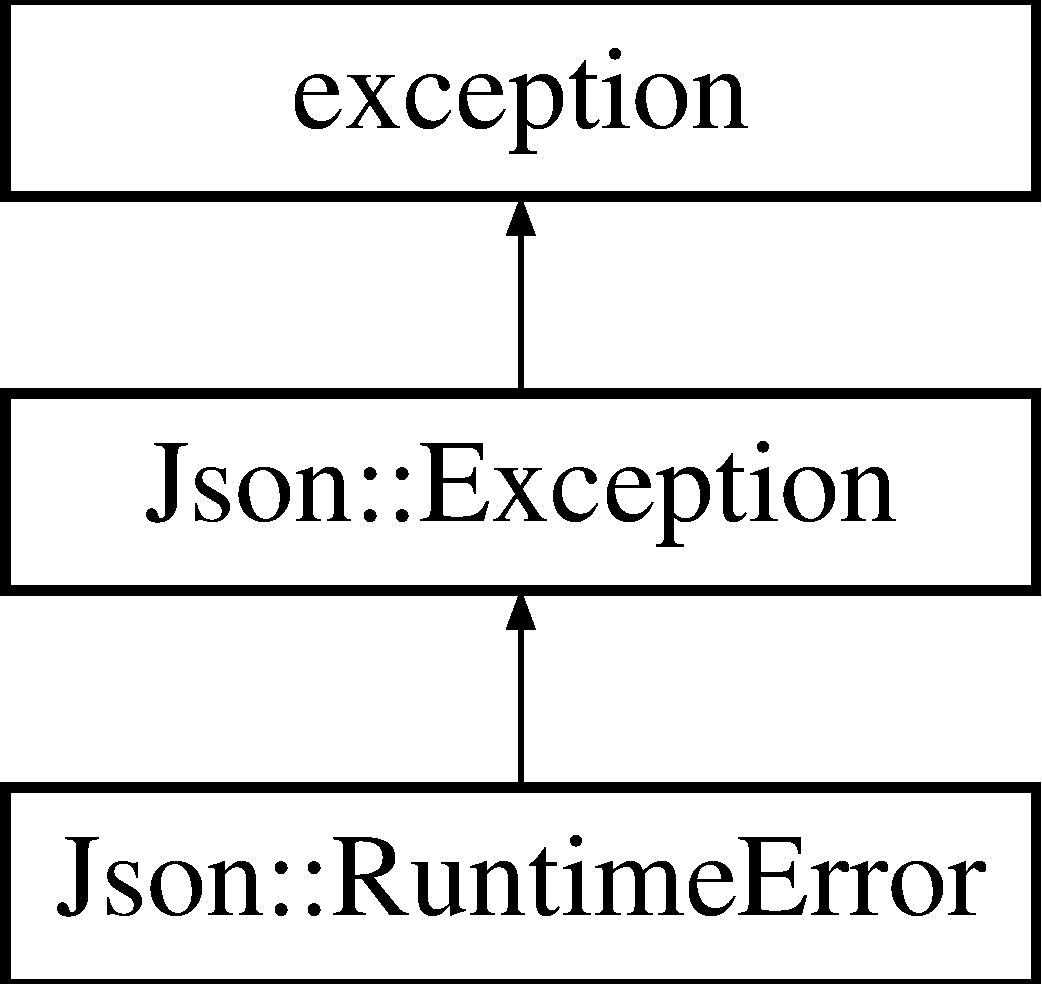
\includegraphics[height=3.000000cm]{classJson_1_1RuntimeError}
\end{center}
\end{figure}
\subsection*{Public Member Functions}
\begin{DoxyCompactItemize}
\item 
\hyperlink{classJson_1_1RuntimeError_a0f6445dc345ce0a703610b6e893fee40}{Runtime\+Error} (\hyperlink{json_8hpp_a1e723f95759de062585bc4a8fd3fa4be}{J\+S\+O\+N\+C\+P\+P\+\_\+\+S\+T\+R\+I\+NG} const \&msg)
\item 
char const $\ast$ \hyperlink{classJson_1_1Exception_a5a9ed7d91b828b9be81706ef9d483ed6}{what} () const \hyperlink{json_8hpp_a824d6199c91488107e443226fa6022c5}{J\+S\+O\+N\+C\+P\+P\+\_\+\+O\+V\+E\+R\+R\+I\+DE}  throw ()
\end{DoxyCompactItemize}
\subsection*{Protected Attributes}
\begin{DoxyCompactItemize}
\item 
\hyperlink{json_8hpp_a1e723f95759de062585bc4a8fd3fa4be}{J\+S\+O\+N\+C\+P\+P\+\_\+\+S\+T\+R\+I\+NG} \hyperlink{classJson_1_1Exception_aae3cbb8b45bf21480f64502a8329659f}{msg\+\_\+}
\end{DoxyCompactItemize}


\subsection{Detailed Description}
Exceptions which the user cannot easily avoid. 

E.\+g. out-\/of-\/memory (when we use malloc), stack-\/overflow, malicious input

\begin{DoxyRemark}{Remarks}
derived from \hyperlink{classJson_1_1Exception}{Json\+::\+Exception} 
\end{DoxyRemark}


\subsection{Constructor \& Destructor Documentation}
\index{Json\+::\+Runtime\+Error@{Json\+::\+Runtime\+Error}!Runtime\+Error@{Runtime\+Error}}
\index{Runtime\+Error@{Runtime\+Error}!Json\+::\+Runtime\+Error@{Json\+::\+Runtime\+Error}}
\subsubsection[{\texorpdfstring{Runtime\+Error(\+J\+S\+O\+N\+C\+P\+P\+\_\+\+S\+T\+R\+I\+N\+G const \&msg)}{RuntimeError(JSONCPP_STRING const &msg)}}]{\setlength{\rightskip}{0pt plus 5cm}Json\+::\+Runtime\+Error\+::\+Runtime\+Error (
\begin{DoxyParamCaption}
\item[{{\bf J\+S\+O\+N\+C\+P\+P\+\_\+\+S\+T\+R\+I\+NG} const \&}]{msg}
\end{DoxyParamCaption}
)}\hypertarget{classJson_1_1RuntimeError_a0f6445dc345ce0a703610b6e893fee40}{}\label{classJson_1_1RuntimeError_a0f6445dc345ce0a703610b6e893fee40}


\subsection{Member Function Documentation}
\index{Json\+::\+Runtime\+Error@{Json\+::\+Runtime\+Error}!what@{what}}
\index{what@{what}!Json\+::\+Runtime\+Error@{Json\+::\+Runtime\+Error}}
\subsubsection[{\texorpdfstring{what() const J\+S\+O\+N\+C\+P\+P\+\_\+\+O\+V\+E\+R\+R\+I\+DE}{what() const JSONCPP_OVERRIDE}}]{\setlength{\rightskip}{0pt plus 5cm}char const $\ast$ Json\+::\+Exception\+::what (
\begin{DoxyParamCaption}
{}
\end{DoxyParamCaption}
) const throw  ) \hspace{0.3cm}{\ttfamily [inherited]}}\hypertarget{classJson_1_1Exception_a5a9ed7d91b828b9be81706ef9d483ed6}{}\label{classJson_1_1Exception_a5a9ed7d91b828b9be81706ef9d483ed6}


\subsection{Member Data Documentation}
\index{Json\+::\+Runtime\+Error@{Json\+::\+Runtime\+Error}!msg\+\_\+@{msg\+\_\+}}
\index{msg\+\_\+@{msg\+\_\+}!Json\+::\+Runtime\+Error@{Json\+::\+Runtime\+Error}}
\subsubsection[{\texorpdfstring{msg\+\_\+}{msg_}}]{\setlength{\rightskip}{0pt plus 5cm}{\bf J\+S\+O\+N\+C\+P\+P\+\_\+\+S\+T\+R\+I\+NG} Json\+::\+Exception\+::msg\+\_\+\hspace{0.3cm}{\ttfamily [protected]}, {\ttfamily [inherited]}}\hypertarget{classJson_1_1Exception_aae3cbb8b45bf21480f64502a8329659f}{}\label{classJson_1_1Exception_aae3cbb8b45bf21480f64502a8329659f}


The documentation for this class was generated from the following files\+:\begin{DoxyCompactItemize}
\item 
/home/pranav/\+Repositories/zcm/include/\hyperlink{json_8hpp}{json.\+hpp}\item 
/home/pranav/\+Repositories/zcm/src/\hyperlink{json_8cpp}{json.\+cpp}\end{DoxyCompactItemize}

\hypertarget{classzcm_1_1Server}{}\section{zcm\+:\+:Server Class Reference}
\label{classzcm_1_1Server}\index{zcm\+::\+Server@{zcm\+::\+Server}}


\hyperlink{classzcm_1_1Server}{Server} class.  




{\ttfamily \#include $<$server.\+hpp$>$}

\subsection*{Public Member Functions}
\begin{DoxyCompactItemize}
\item 
\hyperlink{classzcm_1_1Server_ab5026e5eebdcf7c5bbfe00dc4cd4f202}{Server} (std\+::string \hyperlink{classzcm_1_1Server_a9d59737b196a7abb3a891dc8723e0dcf}{name}, unsigned int \hyperlink{classzcm_1_1Server_ad088a068dc025ff7aa4bf560cc7c43c1}{priority}, std\+::function$<$ std\+::string(const std\+::string \&)$>$ \hyperlink{classzcm_1_1Server_a287609eb19370fe01adf47f26633ce01}{operation\+\_\+function}, \hyperlink{classzcm_1_1Operation__Queue}{Operation\+\_\+\+Queue} $\ast$\hyperlink{classzcm_1_1Server_a667c0fef537aa6acc6245d956250c860}{operation\+\_\+queue\+\_\+ptr})
\begin{DoxyCompactList}\small\item\em Construct a server object. \end{DoxyCompactList}\item 
\hyperlink{classzcm_1_1Server_a79dae6a2cac7751c71e11a53ec506a8c}{Server} (std\+::string \hyperlink{classzcm_1_1Server_a9d59737b196a7abb3a891dc8723e0dcf}{name}, unsigned int \hyperlink{classzcm_1_1Server_ad088a068dc025ff7aa4bf560cc7c43c1}{priority}, std\+::vector$<$ std\+::string $>$ \hyperlink{classzcm_1_1Server_a488d1398b76851565a4d116f7cf72af1}{endpoints}, std\+::function$<$ std\+::string(const std\+::string \&)$>$ \hyperlink{classzcm_1_1Server_a287609eb19370fe01adf47f26633ce01}{operation\+\_\+function}, \hyperlink{classzcm_1_1Operation__Queue}{Operation\+\_\+\+Queue} $\ast$\hyperlink{classzcm_1_1Server_a667c0fef537aa6acc6245d956250c860}{operation\+\_\+queue\+\_\+ptr})
\begin{DoxyCompactList}\small\item\em Construct a server object with known endpoints. \end{DoxyCompactList}\item 
\hyperlink{classzcm_1_1Server_a1aac28d71da6d5e66fff629d7206b3c6}{$\sim$\+Server} ()
\begin{DoxyCompactList}\small\item\em Close the server socket and destroy the Z\+MQ context. \end{DoxyCompactList}\item 
void \hyperlink{classzcm_1_1Server_a663b9c844bd17d3174cdfe367fe7d2e2}{bind} (std\+::vector$<$ std\+::string $>$ new\+\_\+endpoints)
\begin{DoxyCompactList}\small\item\em Bind to a new set of endpoints param\mbox{[}in\mbox{]} new\+\_\+endpoints A new vector of endpoints to bind to. \end{DoxyCompactList}\item 
std\+::string \hyperlink{classzcm_1_1Server_adff186f44785ea8c17f3d96cf8e254e6}{get\+\_\+name} ()
\begin{DoxyCompactList}\small\item\em Get the name of the server. \end{DoxyCompactList}\item 
unsigned int \hyperlink{classzcm_1_1Server_ae570e2fe8f61761951d79c9c5b6ea988}{get\+\_\+priority} ()
\begin{DoxyCompactList}\small\item\em Get the priority of the server. \end{DoxyCompactList}\item 
void \hyperlink{classzcm_1_1Server_ad1c5e86ea9384c95774046ac469092b7}{add\+\_\+connection} (std\+::string new\+\_\+connection)
\begin{DoxyCompactList}\small\item\em Add a new connection to the server. \end{DoxyCompactList}\item 
void \hyperlink{classzcm_1_1Server_ae30eb0c0b4cfad74b7f73c17815511eb}{recv} ()
\begin{DoxyCompactList}\small\item\em Thread function of the server Behavior\+: (1) Wait for a new request on the server Z\+MQ socket (2) Create a \hyperlink{classzcm_1_1Server}{Server} Operation (3) Enqueue onto operation\+\_\+queue (4) Goto step (1) \end{DoxyCompactList}\item 
void \hyperlink{classzcm_1_1Server_ae76811b738db33b85e5c39307f08c5e2}{rebind\+\_\+operation\+\_\+function} (std\+::function$<$ std\+::string(const std\+::string \&)$>$ new\+\_\+operation\+\_\+function)
\begin{DoxyCompactList}\small\item\em Rebind the server operation function. \end{DoxyCompactList}\item 
std\+::thread \hyperlink{classzcm_1_1Server_a77c0b86016dce3e6cef6a64118edd584}{spawn} ()
\begin{DoxyCompactList}\small\item\em Spawn a new thread for the server. \end{DoxyCompactList}\item 
void \hyperlink{classzcm_1_1Server_ab94400c32a097989a769cfb1d77936b4}{start} ()
\begin{DoxyCompactList}\small\item\em Start the server thread. \end{DoxyCompactList}\end{DoxyCompactItemize}
\subsection*{Private Attributes}
\begin{DoxyCompactItemize}
\item 
std\+::string \hyperlink{classzcm_1_1Server_a9d59737b196a7abb3a891dc8723e0dcf}{name}
\begin{DoxyCompactList}\small\item\em Name of the server. \end{DoxyCompactList}\item 
unsigned int \hyperlink{classzcm_1_1Server_ad088a068dc025ff7aa4bf560cc7c43c1}{priority}
\begin{DoxyCompactList}\small\item\em Priority of the server. \end{DoxyCompactList}\item 
std\+::vector$<$ std\+::string $>$ \hyperlink{classzcm_1_1Server_a488d1398b76851565a4d116f7cf72af1}{endpoints}
\begin{DoxyCompactList}\small\item\em Vector of connection endpoints. \end{DoxyCompactList}\item 
std\+::function$<$ std\+::string(const std\+::string \&)$>$ \hyperlink{classzcm_1_1Server_a287609eb19370fe01adf47f26633ce01}{operation\+\_\+function}
\begin{DoxyCompactList}\small\item\em Operation function bound to the server -\/ \hyperlink{classzcm_1_1Component}{Component} method that handles received requests. \end{DoxyCompactList}\item 
\hyperlink{classzcm_1_1Operation__Queue}{Operation\+\_\+\+Queue} $\ast$ \hyperlink{classzcm_1_1Server_a667c0fef537aa6acc6245d956250c860}{operation\+\_\+queue\+\_\+ptr}
\begin{DoxyCompactList}\small\item\em Pointer to the operation\+\_\+queue. \end{DoxyCompactList}\item 
zmq\+::context\+\_\+t $\ast$ \hyperlink{classzcm_1_1Server_a2de8909537ebb88665bfcca1f931c2f8}{context}
\begin{DoxyCompactList}\small\item\em Pointer to the server Z\+MQ context. \end{DoxyCompactList}\item 
zmq\+::socket\+\_\+t $\ast$ \hyperlink{classzcm_1_1Server_a4312bf38cfd6bb1d169d6bd3682651e3}{server\+\_\+socket}
\begin{DoxyCompactList}\small\item\em Pointer to the server Z\+MQ socket. \end{DoxyCompactList}\item 
bool \hyperlink{classzcm_1_1Server_a709ad2426e77a5e442d70a762cbe504b}{ready}
\begin{DoxyCompactList}\small\item\em Boolean representing the state of the server to receive new requests. \end{DoxyCompactList}\item 
std\+::mutex \hyperlink{classzcm_1_1Server_a3e36a37479457237786db9e163d6fef0}{func\+\_\+mutex}
\begin{DoxyCompactList}\small\item\em Mutex used when changing operation\+\_\+function at runtime. \end{DoxyCompactList}\end{DoxyCompactItemize}


\subsection{Detailed Description}
\hyperlink{classzcm_1_1Server}{Server} class. 

\subsection{Constructor \& Destructor Documentation}
\index{zcm\+::\+Server@{zcm\+::\+Server}!Server@{Server}}
\index{Server@{Server}!zcm\+::\+Server@{zcm\+::\+Server}}
\subsubsection[{\texorpdfstring{Server(std\+::string name, unsigned int priority, std\+::function$<$ std\+::string(const std\+::string \&)$>$ operation\+\_\+function, Operation\+\_\+\+Queue $\ast$operation\+\_\+queue\+\_\+ptr)}{Server(std::string name, unsigned int priority, std::function< std::string(const std::string &)> operation_function, Operation_Queue *operation_queue_ptr)}}]{\setlength{\rightskip}{0pt plus 5cm}zcm\+::\+Server\+::\+Server (
\begin{DoxyParamCaption}
\item[{std\+::string}]{name, }
\item[{unsigned int}]{priority, }
\item[{std\+::function$<$ std\+::string(const std\+::string \&)$>$}]{operation\+\_\+function, }
\item[{{\bf Operation\+\_\+\+Queue} $\ast$}]{operation\+\_\+queue\+\_\+ptr}
\end{DoxyParamCaption}
)\hspace{0.3cm}{\ttfamily [inline]}}\hypertarget{classzcm_1_1Server_ab5026e5eebdcf7c5bbfe00dc4cd4f202}{}\label{classzcm_1_1Server_ab5026e5eebdcf7c5bbfe00dc4cd4f202}


Construct a server object. 


\begin{DoxyParams}[1]{Parameters}
\mbox{\tt in}  & {\em name} & \hyperlink{classzcm_1_1Server}{Server} name \\
\hline
\mbox{\tt in}  & {\em priority} & Priority of the server \\
\hline
\mbox{\tt in}  & {\em operation\+\_\+function} & Operation function of the server \\
\hline
\mbox{\tt in}  & {\em operation\+\_\+queue\+\_\+ptr} & Pointer to the operation queue \\
\hline
\end{DoxyParams}
\index{zcm\+::\+Server@{zcm\+::\+Server}!Server@{Server}}
\index{Server@{Server}!zcm\+::\+Server@{zcm\+::\+Server}}
\subsubsection[{\texorpdfstring{Server(std\+::string name, unsigned int priority, std\+::vector$<$ std\+::string $>$ endpoints, std\+::function$<$ std\+::string(const std\+::string \&)$>$ operation\+\_\+function, Operation\+\_\+\+Queue $\ast$operation\+\_\+queue\+\_\+ptr)}{Server(std::string name, unsigned int priority, std::vector< std::string > endpoints, std::function< std::string(const std::string &)> operation_function, Operation_Queue *operation_queue_ptr)}}]{\setlength{\rightskip}{0pt plus 5cm}zcm\+::\+Server\+::\+Server (
\begin{DoxyParamCaption}
\item[{std\+::string}]{name, }
\item[{unsigned int}]{priority, }
\item[{std\+::vector$<$ std\+::string $>$}]{endpoints, }
\item[{std\+::function$<$ std\+::string(const std\+::string \&)$>$}]{operation\+\_\+function, }
\item[{{\bf Operation\+\_\+\+Queue} $\ast$}]{operation\+\_\+queue\+\_\+ptr}
\end{DoxyParamCaption}
)}\hypertarget{classzcm_1_1Server_a79dae6a2cac7751c71e11a53ec506a8c}{}\label{classzcm_1_1Server_a79dae6a2cac7751c71e11a53ec506a8c}


Construct a server object with known endpoints. 


\begin{DoxyParams}[1]{Parameters}
\mbox{\tt in}  & {\em name} & \hyperlink{classzcm_1_1Server}{Server} name \\
\hline
\mbox{\tt in}  & {\em priority} & Priority of the server \\
\hline
\mbox{\tt in}  & {\em endpoints} & A vector of endpoints to bind to \\
\hline
\mbox{\tt in}  & {\em operation\+\_\+function} & Operation function of the server \\
\hline
\mbox{\tt in}  & {\em operation\+\_\+queue\+\_\+ptr} & Pointer to the operation queue \\
\hline
\end{DoxyParams}
\index{zcm\+::\+Server@{zcm\+::\+Server}!````~Server@{$\sim$\+Server}}
\index{````~Server@{$\sim$\+Server}!zcm\+::\+Server@{zcm\+::\+Server}}
\subsubsection[{\texorpdfstring{$\sim$\+Server()}{~Server()}}]{\setlength{\rightskip}{0pt plus 5cm}zcm\+::\+Server\+::$\sim$\+Server (
\begin{DoxyParamCaption}
{}
\end{DoxyParamCaption}
)}\hypertarget{classzcm_1_1Server_a1aac28d71da6d5e66fff629d7206b3c6}{}\label{classzcm_1_1Server_a1aac28d71da6d5e66fff629d7206b3c6}


Close the server socket and destroy the Z\+MQ context. 



\subsection{Member Function Documentation}
\index{zcm\+::\+Server@{zcm\+::\+Server}!add\+\_\+connection@{add\+\_\+connection}}
\index{add\+\_\+connection@{add\+\_\+connection}!zcm\+::\+Server@{zcm\+::\+Server}}
\subsubsection[{\texorpdfstring{add\+\_\+connection(std\+::string new\+\_\+connection)}{add_connection(std::string new_connection)}}]{\setlength{\rightskip}{0pt plus 5cm}void zcm\+::\+Server\+::add\+\_\+connection (
\begin{DoxyParamCaption}
\item[{std\+::string}]{new\+\_\+connection}
\end{DoxyParamCaption}
)}\hypertarget{classzcm_1_1Server_ad1c5e86ea9384c95774046ac469092b7}{}\label{classzcm_1_1Server_ad1c5e86ea9384c95774046ac469092b7}


Add a new connection to the server. 


\begin{DoxyParams}[1]{Parameters}
\mbox{\tt in}  & {\em new\+\_\+connection} & New connection address to bind to \\
\hline
\end{DoxyParams}
\index{zcm\+::\+Server@{zcm\+::\+Server}!bind@{bind}}
\index{bind@{bind}!zcm\+::\+Server@{zcm\+::\+Server}}
\subsubsection[{\texorpdfstring{bind(std\+::vector$<$ std\+::string $>$ new\+\_\+endpoints)}{bind(std::vector< std::string > new_endpoints)}}]{\setlength{\rightskip}{0pt plus 5cm}void zcm\+::\+Server\+::bind (
\begin{DoxyParamCaption}
\item[{std\+::vector$<$ std\+::string $>$}]{new\+\_\+endpoints}
\end{DoxyParamCaption}
)}\hypertarget{classzcm_1_1Server_a663b9c844bd17d3174cdfe367fe7d2e2}{}\label{classzcm_1_1Server_a663b9c844bd17d3174cdfe367fe7d2e2}


Bind to a new set of endpoints param\mbox{[}in\mbox{]} new\+\_\+endpoints A new vector of endpoints to bind to. 

\index{zcm\+::\+Server@{zcm\+::\+Server}!get\+\_\+name@{get\+\_\+name}}
\index{get\+\_\+name@{get\+\_\+name}!zcm\+::\+Server@{zcm\+::\+Server}}
\subsubsection[{\texorpdfstring{get\+\_\+name()}{get_name()}}]{\setlength{\rightskip}{0pt plus 5cm}std\+::string zcm\+::\+Server\+::get\+\_\+name (
\begin{DoxyParamCaption}
{}
\end{DoxyParamCaption}
)}\hypertarget{classzcm_1_1Server_adff186f44785ea8c17f3d96cf8e254e6}{}\label{classzcm_1_1Server_adff186f44785ea8c17f3d96cf8e254e6}


Get the name of the server. 

\index{zcm\+::\+Server@{zcm\+::\+Server}!get\+\_\+priority@{get\+\_\+priority}}
\index{get\+\_\+priority@{get\+\_\+priority}!zcm\+::\+Server@{zcm\+::\+Server}}
\subsubsection[{\texorpdfstring{get\+\_\+priority()}{get_priority()}}]{\setlength{\rightskip}{0pt plus 5cm}unsigned int zcm\+::\+Server\+::get\+\_\+priority (
\begin{DoxyParamCaption}
{}
\end{DoxyParamCaption}
)}\hypertarget{classzcm_1_1Server_ae570e2fe8f61761951d79c9c5b6ea988}{}\label{classzcm_1_1Server_ae570e2fe8f61761951d79c9c5b6ea988}


Get the priority of the server. 

\index{zcm\+::\+Server@{zcm\+::\+Server}!rebind\+\_\+operation\+\_\+function@{rebind\+\_\+operation\+\_\+function}}
\index{rebind\+\_\+operation\+\_\+function@{rebind\+\_\+operation\+\_\+function}!zcm\+::\+Server@{zcm\+::\+Server}}
\subsubsection[{\texorpdfstring{rebind\+\_\+operation\+\_\+function(std\+::function$<$ std\+::string(const std\+::string \&)$>$ new\+\_\+operation\+\_\+function)}{rebind_operation_function(std::function< std::string(const std::string &)> new_operation_function)}}]{\setlength{\rightskip}{0pt plus 5cm}void zcm\+::\+Server\+::rebind\+\_\+operation\+\_\+function (
\begin{DoxyParamCaption}
\item[{std\+::function$<$ std\+::string(const std\+::string \&)$>$}]{new\+\_\+operation\+\_\+function}
\end{DoxyParamCaption}
)}\hypertarget{classzcm_1_1Server_ae76811b738db33b85e5c39307f08c5e2}{}\label{classzcm_1_1Server_ae76811b738db33b85e5c39307f08c5e2}


Rebind the server operation function. 


\begin{DoxyParams}[1]{Parameters}
\mbox{\tt in}  & {\em new\+\_\+operation\+\_\+function} & New server function to be handled upon \hyperlink{classzcm_1_1Server_ae30eb0c0b4cfad74b7f73c17815511eb}{recv()} \\
\hline
\end{DoxyParams}
\index{zcm\+::\+Server@{zcm\+::\+Server}!recv@{recv}}
\index{recv@{recv}!zcm\+::\+Server@{zcm\+::\+Server}}
\subsubsection[{\texorpdfstring{recv()}{recv()}}]{\setlength{\rightskip}{0pt plus 5cm}void zcm\+::\+Server\+::recv (
\begin{DoxyParamCaption}
{}
\end{DoxyParamCaption}
)}\hypertarget{classzcm_1_1Server_ae30eb0c0b4cfad74b7f73c17815511eb}{}\label{classzcm_1_1Server_ae30eb0c0b4cfad74b7f73c17815511eb}


Thread function of the server Behavior\+: (1) Wait for a new request on the server Z\+MQ socket (2) Create a \hyperlink{classzcm_1_1Server}{Server} Operation (3) Enqueue onto operation\+\_\+queue (4) Goto step (1) 

\index{zcm\+::\+Server@{zcm\+::\+Server}!spawn@{spawn}}
\index{spawn@{spawn}!zcm\+::\+Server@{zcm\+::\+Server}}
\subsubsection[{\texorpdfstring{spawn()}{spawn()}}]{\setlength{\rightskip}{0pt plus 5cm}std\+::thread zcm\+::\+Server\+::spawn (
\begin{DoxyParamCaption}
{}
\end{DoxyParamCaption}
)}\hypertarget{classzcm_1_1Server_a77c0b86016dce3e6cef6a64118edd584}{}\label{classzcm_1_1Server_a77c0b86016dce3e6cef6a64118edd584}


Spawn a new thread for the server. 

\begin{DoxyReturn}{Returns}
\hyperlink{classzcm_1_1Server}{Server} thread 
\end{DoxyReturn}
\index{zcm\+::\+Server@{zcm\+::\+Server}!start@{start}}
\index{start@{start}!zcm\+::\+Server@{zcm\+::\+Server}}
\subsubsection[{\texorpdfstring{start()}{start()}}]{\setlength{\rightskip}{0pt plus 5cm}void zcm\+::\+Server\+::start (
\begin{DoxyParamCaption}
{}
\end{DoxyParamCaption}
)}\hypertarget{classzcm_1_1Server_ab94400c32a097989a769cfb1d77936b4}{}\label{classzcm_1_1Server_ab94400c32a097989a769cfb1d77936b4}


Start the server thread. 



\subsection{Member Data Documentation}
\index{zcm\+::\+Server@{zcm\+::\+Server}!context@{context}}
\index{context@{context}!zcm\+::\+Server@{zcm\+::\+Server}}
\subsubsection[{\texorpdfstring{context}{context}}]{\setlength{\rightskip}{0pt plus 5cm}zmq\+::context\+\_\+t$\ast$ zcm\+::\+Server\+::context\hspace{0.3cm}{\ttfamily [private]}}\hypertarget{classzcm_1_1Server_a2de8909537ebb88665bfcca1f931c2f8}{}\label{classzcm_1_1Server_a2de8909537ebb88665bfcca1f931c2f8}


Pointer to the server Z\+MQ context. 

\index{zcm\+::\+Server@{zcm\+::\+Server}!endpoints@{endpoints}}
\index{endpoints@{endpoints}!zcm\+::\+Server@{zcm\+::\+Server}}
\subsubsection[{\texorpdfstring{endpoints}{endpoints}}]{\setlength{\rightskip}{0pt plus 5cm}std\+::vector$<$std\+::string$>$ zcm\+::\+Server\+::endpoints\hspace{0.3cm}{\ttfamily [private]}}\hypertarget{classzcm_1_1Server_a488d1398b76851565a4d116f7cf72af1}{}\label{classzcm_1_1Server_a488d1398b76851565a4d116f7cf72af1}


Vector of connection endpoints. 

\index{zcm\+::\+Server@{zcm\+::\+Server}!func\+\_\+mutex@{func\+\_\+mutex}}
\index{func\+\_\+mutex@{func\+\_\+mutex}!zcm\+::\+Server@{zcm\+::\+Server}}
\subsubsection[{\texorpdfstring{func\+\_\+mutex}{func_mutex}}]{\setlength{\rightskip}{0pt plus 5cm}std\+::mutex zcm\+::\+Server\+::func\+\_\+mutex\hspace{0.3cm}{\ttfamily [private]}}\hypertarget{classzcm_1_1Server_a3e36a37479457237786db9e163d6fef0}{}\label{classzcm_1_1Server_a3e36a37479457237786db9e163d6fef0}


Mutex used when changing operation\+\_\+function at runtime. 

\index{zcm\+::\+Server@{zcm\+::\+Server}!name@{name}}
\index{name@{name}!zcm\+::\+Server@{zcm\+::\+Server}}
\subsubsection[{\texorpdfstring{name}{name}}]{\setlength{\rightskip}{0pt plus 5cm}std\+::string zcm\+::\+Server\+::name\hspace{0.3cm}{\ttfamily [private]}}\hypertarget{classzcm_1_1Server_a9d59737b196a7abb3a891dc8723e0dcf}{}\label{classzcm_1_1Server_a9d59737b196a7abb3a891dc8723e0dcf}


Name of the server. 

\index{zcm\+::\+Server@{zcm\+::\+Server}!operation\+\_\+function@{operation\+\_\+function}}
\index{operation\+\_\+function@{operation\+\_\+function}!zcm\+::\+Server@{zcm\+::\+Server}}
\subsubsection[{\texorpdfstring{operation\+\_\+function}{operation_function}}]{\setlength{\rightskip}{0pt plus 5cm}std\+::function$<$std\+::string(const std\+::string\&)$>$ zcm\+::\+Server\+::operation\+\_\+function\hspace{0.3cm}{\ttfamily [private]}}\hypertarget{classzcm_1_1Server_a287609eb19370fe01adf47f26633ce01}{}\label{classzcm_1_1Server_a287609eb19370fe01adf47f26633ce01}


Operation function bound to the server -\/ \hyperlink{classzcm_1_1Component}{Component} method that handles received requests. 

\index{zcm\+::\+Server@{zcm\+::\+Server}!operation\+\_\+queue\+\_\+ptr@{operation\+\_\+queue\+\_\+ptr}}
\index{operation\+\_\+queue\+\_\+ptr@{operation\+\_\+queue\+\_\+ptr}!zcm\+::\+Server@{zcm\+::\+Server}}
\subsubsection[{\texorpdfstring{operation\+\_\+queue\+\_\+ptr}{operation_queue_ptr}}]{\setlength{\rightskip}{0pt plus 5cm}{\bf Operation\+\_\+\+Queue}$\ast$ zcm\+::\+Server\+::operation\+\_\+queue\+\_\+ptr\hspace{0.3cm}{\ttfamily [private]}}\hypertarget{classzcm_1_1Server_a667c0fef537aa6acc6245d956250c860}{}\label{classzcm_1_1Server_a667c0fef537aa6acc6245d956250c860}


Pointer to the operation\+\_\+queue. 

\index{zcm\+::\+Server@{zcm\+::\+Server}!priority@{priority}}
\index{priority@{priority}!zcm\+::\+Server@{zcm\+::\+Server}}
\subsubsection[{\texorpdfstring{priority}{priority}}]{\setlength{\rightskip}{0pt plus 5cm}unsigned int zcm\+::\+Server\+::priority\hspace{0.3cm}{\ttfamily [private]}}\hypertarget{classzcm_1_1Server_ad088a068dc025ff7aa4bf560cc7c43c1}{}\label{classzcm_1_1Server_ad088a068dc025ff7aa4bf560cc7c43c1}


Priority of the server. 

\index{zcm\+::\+Server@{zcm\+::\+Server}!ready@{ready}}
\index{ready@{ready}!zcm\+::\+Server@{zcm\+::\+Server}}
\subsubsection[{\texorpdfstring{ready}{ready}}]{\setlength{\rightskip}{0pt plus 5cm}bool zcm\+::\+Server\+::ready\hspace{0.3cm}{\ttfamily [private]}}\hypertarget{classzcm_1_1Server_a709ad2426e77a5e442d70a762cbe504b}{}\label{classzcm_1_1Server_a709ad2426e77a5e442d70a762cbe504b}


Boolean representing the state of the server to receive new requests. 

\index{zcm\+::\+Server@{zcm\+::\+Server}!server\+\_\+socket@{server\+\_\+socket}}
\index{server\+\_\+socket@{server\+\_\+socket}!zcm\+::\+Server@{zcm\+::\+Server}}
\subsubsection[{\texorpdfstring{server\+\_\+socket}{server_socket}}]{\setlength{\rightskip}{0pt plus 5cm}zmq\+::socket\+\_\+t$\ast$ zcm\+::\+Server\+::server\+\_\+socket\hspace{0.3cm}{\ttfamily [private]}}\hypertarget{classzcm_1_1Server_a4312bf38cfd6bb1d169d6bd3682651e3}{}\label{classzcm_1_1Server_a4312bf38cfd6bb1d169d6bd3682651e3}


Pointer to the server Z\+MQ socket. 



The documentation for this class was generated from the following files\+:\begin{DoxyCompactItemize}
\item 
/home/pranav/\+Repositories/zcm/include/\hyperlink{server_8hpp}{server.\+hpp}\item 
/home/pranav/\+Repositories/zcm/src/\hyperlink{server_8cpp}{server.\+cpp}\end{DoxyCompactItemize}

\hypertarget{classzcm_1_1Server__Operation}{}\section{zcm\+:\+:Server\+\_\+\+Operation Class Reference}
\label{classzcm_1_1Server__Operation}\index{zcm\+::\+Server\+\_\+\+Operation@{zcm\+::\+Server\+\_\+\+Operation}}


\hyperlink{classzcm_1_1Server}{Server} Operation class.  




{\ttfamily \#include $<$operation\+\_\+types.\+hpp$>$}

Inheritance diagram for zcm\+:\+:Server\+\_\+\+Operation\+:\begin{figure}[H]
\begin{center}
\leavevmode
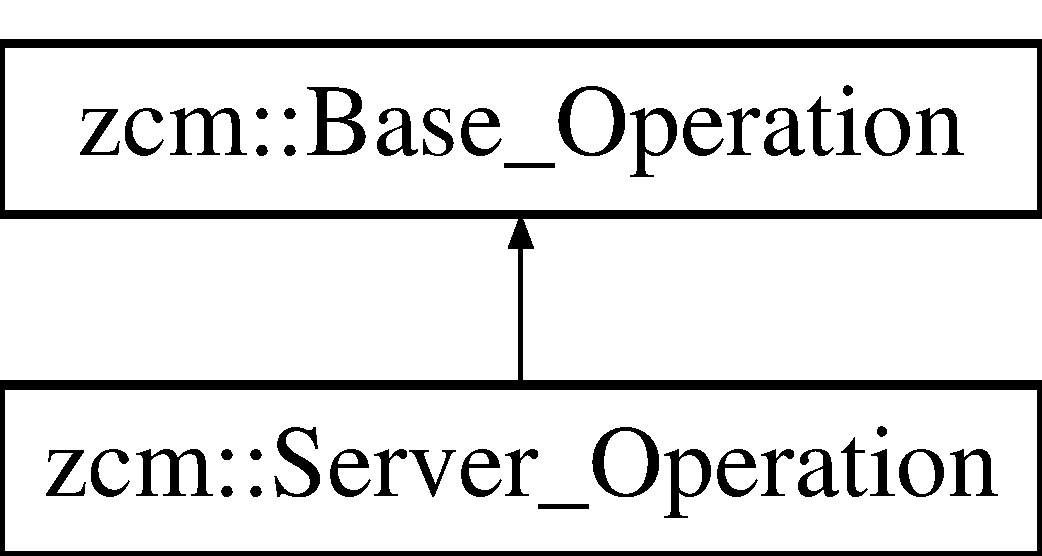
\includegraphics[height=2.000000cm]{classzcm_1_1Server__Operation}
\end{center}
\end{figure}
\subsection*{Public Member Functions}
\begin{DoxyCompactItemize}
\item 
\hyperlink{classzcm_1_1Server__Operation_a8457695fe5f8f3416106596597695406}{Server\+\_\+\+Operation} (std\+::string \hyperlink{classzcm_1_1Base__Operation_a2e2192550818d8f063fc7b2c76c5e21c}{name}, unsigned int \hyperlink{classzcm_1_1Base__Operation_a38af3bcc2578ef215772d595bf3fa358}{priority}, std\+::function$<$ std\+::string()$>$ \hyperlink{classzcm_1_1Server__Operation_a9fe0d75b858647a21323293746df6c9e}{operation\+\_\+function}, zmq\+::socket\+\_\+t $\ast$\hyperlink{classzcm_1_1Server__Operation_a07efad79c512d03a54fe2bb99166d52f}{socket\+\_\+ptr}, bool $\ast$\hyperlink{classzcm_1_1Server__Operation_a2b71778be842aedf6d122b531e186ca8}{recv\+\_\+ready})
\begin{DoxyCompactList}\small\item\em Construct a server operation. \end{DoxyCompactList}\item 
void \hyperlink{classzcm_1_1Server__Operation_acd6b89c42aad3df5dc78674770326498}{execute} ()
\begin{DoxyCompactList}\small\item\em \hyperlink{classzcm_1_1Server}{Server} operation function. \end{DoxyCompactList}\item 
zmq\+::socket\+\_\+t $\ast$ \hyperlink{classzcm_1_1Server__Operation_a17d90d76a8cfa0dc25792144e155e7c0}{get\+\_\+socket\+\_\+ptr} ()
\begin{DoxyCompactList}\small\item\em Get the Z\+MQ server socket pointer. \end{DoxyCompactList}\item 
void \hyperlink{classzcm_1_1Server__Operation_a1477e76e1639bdebc6b855d3be4e9fb2}{set\+\_\+ready} ()
\begin{DoxyCompactList}\small\item\em Get the Z\+MQ server \char`\"{}ready\char`\"{} variable. \end{DoxyCompactList}\item 
std\+::string \hyperlink{classzcm_1_1Base__Operation_a46b6a3f23e18bc35425ec2dab80c849f}{get\+\_\+name} ()
\begin{DoxyCompactList}\small\item\em Return the operation name. \end{DoxyCompactList}\item 
unsigned int \hyperlink{classzcm_1_1Base__Operation_a3b15b35c31ed173d2abb193e9fba32ef}{get\+\_\+priority} () const 
\begin{DoxyCompactList}\small\item\em Return the operation priority. \end{DoxyCompactList}\end{DoxyCompactItemize}
\subsection*{Private Attributes}
\begin{DoxyCompactItemize}
\item 
std\+::function$<$ std\+::string()$>$ \hyperlink{classzcm_1_1Server__Operation_a9fe0d75b858647a21323293746df6c9e}{operation\+\_\+function}
\begin{DoxyCompactList}\small\item\em \hyperlink{classzcm_1_1Server}{Server} Operation Function. \end{DoxyCompactList}\item 
zmq\+::socket\+\_\+t $\ast$ \hyperlink{classzcm_1_1Server__Operation_a07efad79c512d03a54fe2bb99166d52f}{socket\+\_\+ptr}
\begin{DoxyCompactList}\small\item\em Pointer to the \hyperlink{classzcm_1_1Server}{Server} Z\+MQ socket. \end{DoxyCompactList}\item 
bool $\ast$ \hyperlink{classzcm_1_1Server__Operation_a2b71778be842aedf6d122b531e186ca8}{recv\+\_\+ready}
\begin{DoxyCompactList}\small\item\em Pointer to the \hyperlink{classzcm_1_1Server}{Server} \char`\"{}ready\char`\"{} variable. \end{DoxyCompactList}\end{DoxyCompactItemize}


\subsection{Detailed Description}
\hyperlink{classzcm_1_1Server}{Server} Operation class. 

\subsection{Constructor \& Destructor Documentation}
\index{zcm\+::\+Server\+\_\+\+Operation@{zcm\+::\+Server\+\_\+\+Operation}!Server\+\_\+\+Operation@{Server\+\_\+\+Operation}}
\index{Server\+\_\+\+Operation@{Server\+\_\+\+Operation}!zcm\+::\+Server\+\_\+\+Operation@{zcm\+::\+Server\+\_\+\+Operation}}
\subsubsection[{\texorpdfstring{Server\+\_\+\+Operation(std\+::string name, unsigned int priority, std\+::function$<$ std\+::string()$>$ operation\+\_\+function, zmq\+::socket\+\_\+t $\ast$socket\+\_\+ptr, bool $\ast$recv\+\_\+ready)}{Server_Operation(std::string name, unsigned int priority, std::function< std::string()> operation_function, zmq::socket_t *socket_ptr, bool *recv_ready)}}]{\setlength{\rightskip}{0pt plus 5cm}zcm\+::\+Server\+\_\+\+Operation\+::\+Server\+\_\+\+Operation (
\begin{DoxyParamCaption}
\item[{std\+::string}]{name, }
\item[{unsigned int}]{priority, }
\item[{std\+::function$<$ std\+::string()$>$}]{operation\+\_\+function, }
\item[{zmq\+::socket\+\_\+t $\ast$}]{socket\+\_\+ptr, }
\item[{bool $\ast$}]{recv\+\_\+ready}
\end{DoxyParamCaption}
)\hspace{0.3cm}{\ttfamily [inline]}}\hypertarget{classzcm_1_1Server__Operation_a8457695fe5f8f3416106596597695406}{}\label{classzcm_1_1Server__Operation_a8457695fe5f8f3416106596597695406}


Construct a server operation. 


\begin{DoxyParams}[1]{Parameters}
\mbox{\tt in}  & {\em name} & Name of the operation \\
\hline
\mbox{\tt in}  & {\em priority} & Priority of the operation \\
\hline
\mbox{\tt in}  & {\em operation\+\_\+function} & \hyperlink{classzcm_1_1Server}{Server} function \\
\hline
\mbox{\tt in}  & {\em socket\+\_\+ptr} & Pointer to the \hyperlink{classzcm_1_1Server}{Server} Z\+MQ socket \\
\hline
\mbox{\tt in}  & {\em recv\+\_\+ready} & Pointer to the \hyperlink{classzcm_1_1Server}{Server} ready variable \\
\hline
\end{DoxyParams}


\subsection{Member Function Documentation}
\index{zcm\+::\+Server\+\_\+\+Operation@{zcm\+::\+Server\+\_\+\+Operation}!execute@{execute}}
\index{execute@{execute}!zcm\+::\+Server\+\_\+\+Operation@{zcm\+::\+Server\+\_\+\+Operation}}
\subsubsection[{\texorpdfstring{execute()}{execute()}}]{\setlength{\rightskip}{0pt plus 5cm}void zcm\+::\+Server\+\_\+\+Operation\+::execute (
\begin{DoxyParamCaption}
{}
\end{DoxyParamCaption}
)\hspace{0.3cm}{\ttfamily [virtual]}}\hypertarget{classzcm_1_1Server__Operation_acd6b89c42aad3df5dc78674770326498}{}\label{classzcm_1_1Server__Operation_acd6b89c42aad3df5dc78674770326498}


\hyperlink{classzcm_1_1Server}{Server} operation function. 



Reimplemented from \hyperlink{classzcm_1_1Base__Operation_a58cb533edd6e6f220d2d1c260fbddca4}{zcm\+::\+Base\+\_\+\+Operation}.

\index{zcm\+::\+Server\+\_\+\+Operation@{zcm\+::\+Server\+\_\+\+Operation}!get\+\_\+name@{get\+\_\+name}}
\index{get\+\_\+name@{get\+\_\+name}!zcm\+::\+Server\+\_\+\+Operation@{zcm\+::\+Server\+\_\+\+Operation}}
\subsubsection[{\texorpdfstring{get\+\_\+name()}{get_name()}}]{\setlength{\rightskip}{0pt plus 5cm}std\+::string zcm\+::\+Base\+\_\+\+Operation\+::get\+\_\+name (
\begin{DoxyParamCaption}
{}
\end{DoxyParamCaption}
)\hspace{0.3cm}{\ttfamily [inherited]}}\hypertarget{classzcm_1_1Base__Operation_a46b6a3f23e18bc35425ec2dab80c849f}{}\label{classzcm_1_1Base__Operation_a46b6a3f23e18bc35425ec2dab80c849f}


Return the operation name. 

\begin{DoxyReturn}{Returns}
Name of the operation 
\end{DoxyReturn}
\index{zcm\+::\+Server\+\_\+\+Operation@{zcm\+::\+Server\+\_\+\+Operation}!get\+\_\+priority@{get\+\_\+priority}}
\index{get\+\_\+priority@{get\+\_\+priority}!zcm\+::\+Server\+\_\+\+Operation@{zcm\+::\+Server\+\_\+\+Operation}}
\subsubsection[{\texorpdfstring{get\+\_\+priority() const }{get_priority() const }}]{\setlength{\rightskip}{0pt plus 5cm}unsigned int zcm\+::\+Base\+\_\+\+Operation\+::get\+\_\+priority (
\begin{DoxyParamCaption}
{}
\end{DoxyParamCaption}
) const\hspace{0.3cm}{\ttfamily [inherited]}}\hypertarget{classzcm_1_1Base__Operation_a3b15b35c31ed173d2abb193e9fba32ef}{}\label{classzcm_1_1Base__Operation_a3b15b35c31ed173d2abb193e9fba32ef}


Return the operation priority. 

\begin{DoxyReturn}{Returns}
Priority of the operation 
\end{DoxyReturn}
\index{zcm\+::\+Server\+\_\+\+Operation@{zcm\+::\+Server\+\_\+\+Operation}!get\+\_\+socket\+\_\+ptr@{get\+\_\+socket\+\_\+ptr}}
\index{get\+\_\+socket\+\_\+ptr@{get\+\_\+socket\+\_\+ptr}!zcm\+::\+Server\+\_\+\+Operation@{zcm\+::\+Server\+\_\+\+Operation}}
\subsubsection[{\texorpdfstring{get\+\_\+socket\+\_\+ptr()}{get_socket_ptr()}}]{\setlength{\rightskip}{0pt plus 5cm}zmq\+::socket\+\_\+t $\ast$ zcm\+::\+Server\+\_\+\+Operation\+::get\+\_\+socket\+\_\+ptr (
\begin{DoxyParamCaption}
{}
\end{DoxyParamCaption}
)}\hypertarget{classzcm_1_1Server__Operation_a17d90d76a8cfa0dc25792144e155e7c0}{}\label{classzcm_1_1Server__Operation_a17d90d76a8cfa0dc25792144e155e7c0}


Get the Z\+MQ server socket pointer. 

\index{zcm\+::\+Server\+\_\+\+Operation@{zcm\+::\+Server\+\_\+\+Operation}!set\+\_\+ready@{set\+\_\+ready}}
\index{set\+\_\+ready@{set\+\_\+ready}!zcm\+::\+Server\+\_\+\+Operation@{zcm\+::\+Server\+\_\+\+Operation}}
\subsubsection[{\texorpdfstring{set\+\_\+ready()}{set_ready()}}]{\setlength{\rightskip}{0pt plus 5cm}void zcm\+::\+Server\+\_\+\+Operation\+::set\+\_\+ready (
\begin{DoxyParamCaption}
{}
\end{DoxyParamCaption}
)}\hypertarget{classzcm_1_1Server__Operation_a1477e76e1639bdebc6b855d3be4e9fb2}{}\label{classzcm_1_1Server__Operation_a1477e76e1639bdebc6b855d3be4e9fb2}


Get the Z\+MQ server \char`\"{}ready\char`\"{} variable. 



\subsection{Member Data Documentation}
\index{zcm\+::\+Server\+\_\+\+Operation@{zcm\+::\+Server\+\_\+\+Operation}!operation\+\_\+function@{operation\+\_\+function}}
\index{operation\+\_\+function@{operation\+\_\+function}!zcm\+::\+Server\+\_\+\+Operation@{zcm\+::\+Server\+\_\+\+Operation}}
\subsubsection[{\texorpdfstring{operation\+\_\+function}{operation_function}}]{\setlength{\rightskip}{0pt plus 5cm}std\+::function$<$std\+::string()$>$ zcm\+::\+Server\+\_\+\+Operation\+::operation\+\_\+function\hspace{0.3cm}{\ttfamily [private]}}\hypertarget{classzcm_1_1Server__Operation_a9fe0d75b858647a21323293746df6c9e}{}\label{classzcm_1_1Server__Operation_a9fe0d75b858647a21323293746df6c9e}


\hyperlink{classzcm_1_1Server}{Server} Operation Function. 

\index{zcm\+::\+Server\+\_\+\+Operation@{zcm\+::\+Server\+\_\+\+Operation}!recv\+\_\+ready@{recv\+\_\+ready}}
\index{recv\+\_\+ready@{recv\+\_\+ready}!zcm\+::\+Server\+\_\+\+Operation@{zcm\+::\+Server\+\_\+\+Operation}}
\subsubsection[{\texorpdfstring{recv\+\_\+ready}{recv_ready}}]{\setlength{\rightskip}{0pt plus 5cm}bool$\ast$ zcm\+::\+Server\+\_\+\+Operation\+::recv\+\_\+ready\hspace{0.3cm}{\ttfamily [private]}}\hypertarget{classzcm_1_1Server__Operation_a2b71778be842aedf6d122b531e186ca8}{}\label{classzcm_1_1Server__Operation_a2b71778be842aedf6d122b531e186ca8}


Pointer to the \hyperlink{classzcm_1_1Server}{Server} \char`\"{}ready\char`\"{} variable. 

\index{zcm\+::\+Server\+\_\+\+Operation@{zcm\+::\+Server\+\_\+\+Operation}!socket\+\_\+ptr@{socket\+\_\+ptr}}
\index{socket\+\_\+ptr@{socket\+\_\+ptr}!zcm\+::\+Server\+\_\+\+Operation@{zcm\+::\+Server\+\_\+\+Operation}}
\subsubsection[{\texorpdfstring{socket\+\_\+ptr}{socket_ptr}}]{\setlength{\rightskip}{0pt plus 5cm}zmq\+::socket\+\_\+t$\ast$ zcm\+::\+Server\+\_\+\+Operation\+::socket\+\_\+ptr\hspace{0.3cm}{\ttfamily [private]}}\hypertarget{classzcm_1_1Server__Operation_a07efad79c512d03a54fe2bb99166d52f}{}\label{classzcm_1_1Server__Operation_a07efad79c512d03a54fe2bb99166d52f}


Pointer to the \hyperlink{classzcm_1_1Server}{Server} Z\+MQ socket. 



The documentation for this class was generated from the following files\+:\begin{DoxyCompactItemize}
\item 
/home/pranav/\+Repositories/zcm/include/\hyperlink{operation__types_8hpp}{operation\+\_\+types.\+hpp}\item 
/home/pranav/\+Repositories/zcm/src/\hyperlink{operation__types_8cpp}{operation\+\_\+types.\+cpp}\end{DoxyCompactItemize}

\hypertarget{classJson_1_1StaticString}{}\section{Json\+:\+:Static\+String Class Reference}
\label{classJson_1_1StaticString}\index{Json\+::\+Static\+String@{Json\+::\+Static\+String}}


Lightweight wrapper to tag static string.  




{\ttfamily \#include $<$json.\+hpp$>$}

\subsection*{Public Member Functions}
\begin{DoxyCompactItemize}
\item 
\hyperlink{classJson_1_1StaticString_afb6baf1ec078ce76f0b0f9b39d19437f}{Static\+String} (const char $\ast$czstring)
\item 
\hyperlink{classJson_1_1StaticString_ac2b334d46bbea4c0227e508fc66433e9}{operator const char $\ast$} () const 
\item 
const char $\ast$ \hyperlink{classJson_1_1StaticString_ab86fc6a3183adf12fdba4b370acf1754}{c\+\_\+str} () const 
\end{DoxyCompactItemize}
\subsection*{Private Attributes}
\begin{DoxyCompactItemize}
\item 
const char $\ast$ \hyperlink{classJson_1_1StaticString_a9f0d9e8caee8f8db14e2c8c24760dffd}{c\+\_\+str\+\_\+}
\end{DoxyCompactItemize}


\subsection{Detailed Description}
Lightweight wrapper to tag static string. 

\hyperlink{classJson_1_1Value}{Value} constructor and object\+Value member assignement takes advantage of the \hyperlink{classJson_1_1StaticString}{Static\+String} and avoid the cost of string duplication when storing the string or the member name.

Example of usage\+: 
\begin{DoxyCode}
\hyperlink{classJson_1_1Value}{Json::Value} aValue( \hyperlink{classJson_1_1StaticString_afb6baf1ec078ce76f0b0f9b39d19437f}{StaticString}(\textcolor{stringliteral}{"some text"}) );
\hyperlink{classJson_1_1Value}{Json::Value} object;
\textcolor{keyword}{static} \textcolor{keyword}{const} \hyperlink{classJson_1_1StaticString_afb6baf1ec078ce76f0b0f9b39d19437f}{StaticString} code(\textcolor{stringliteral}{"code"});
\textcolor{keywordtype}{object}[code] = 1234;
\end{DoxyCode}
 

\subsection{Constructor \& Destructor Documentation}
\index{Json\+::\+Static\+String@{Json\+::\+Static\+String}!Static\+String@{Static\+String}}
\index{Static\+String@{Static\+String}!Json\+::\+Static\+String@{Json\+::\+Static\+String}}
\subsubsection[{\texorpdfstring{Static\+String(const char $\ast$czstring)}{StaticString(const char *czstring)}}]{\setlength{\rightskip}{0pt plus 5cm}Json\+::\+Static\+String\+::\+Static\+String (
\begin{DoxyParamCaption}
\item[{const char $\ast$}]{czstring}
\end{DoxyParamCaption}
)\hspace{0.3cm}{\ttfamily [inline]}, {\ttfamily [explicit]}}\hypertarget{classJson_1_1StaticString_afb6baf1ec078ce76f0b0f9b39d19437f}{}\label{classJson_1_1StaticString_afb6baf1ec078ce76f0b0f9b39d19437f}


\subsection{Member Function Documentation}
\index{Json\+::\+Static\+String@{Json\+::\+Static\+String}!c\+\_\+str@{c\+\_\+str}}
\index{c\+\_\+str@{c\+\_\+str}!Json\+::\+Static\+String@{Json\+::\+Static\+String}}
\subsubsection[{\texorpdfstring{c\+\_\+str() const }{c_str() const }}]{\setlength{\rightskip}{0pt plus 5cm}const char$\ast$ Json\+::\+Static\+String\+::c\+\_\+str (
\begin{DoxyParamCaption}
{}
\end{DoxyParamCaption}
) const\hspace{0.3cm}{\ttfamily [inline]}}\hypertarget{classJson_1_1StaticString_ab86fc6a3183adf12fdba4b370acf1754}{}\label{classJson_1_1StaticString_ab86fc6a3183adf12fdba4b370acf1754}
\index{Json\+::\+Static\+String@{Json\+::\+Static\+String}!operator const char $\ast$@{operator const char $\ast$}}
\index{operator const char $\ast$@{operator const char $\ast$}!Json\+::\+Static\+String@{Json\+::\+Static\+String}}
\subsubsection[{\texorpdfstring{operator const char $\ast$() const }{operator const char *() const }}]{\setlength{\rightskip}{0pt plus 5cm}Json\+::\+Static\+String\+::operator const char $\ast$ (
\begin{DoxyParamCaption}
{}
\end{DoxyParamCaption}
) const\hspace{0.3cm}{\ttfamily [inline]}}\hypertarget{classJson_1_1StaticString_ac2b334d46bbea4c0227e508fc66433e9}{}\label{classJson_1_1StaticString_ac2b334d46bbea4c0227e508fc66433e9}


\subsection{Member Data Documentation}
\index{Json\+::\+Static\+String@{Json\+::\+Static\+String}!c\+\_\+str\+\_\+@{c\+\_\+str\+\_\+}}
\index{c\+\_\+str\+\_\+@{c\+\_\+str\+\_\+}!Json\+::\+Static\+String@{Json\+::\+Static\+String}}
\subsubsection[{\texorpdfstring{c\+\_\+str\+\_\+}{c_str_}}]{\setlength{\rightskip}{0pt plus 5cm}const char$\ast$ Json\+::\+Static\+String\+::c\+\_\+str\+\_\+\hspace{0.3cm}{\ttfamily [private]}}\hypertarget{classJson_1_1StaticString_a9f0d9e8caee8f8db14e2c8c24760dffd}{}\label{classJson_1_1StaticString_a9f0d9e8caee8f8db14e2c8c24760dffd}


The documentation for this class was generated from the following file\+:\begin{DoxyCompactItemize}
\item 
/home/pranav/\+Repositories/zcm/include/\hyperlink{json_8hpp}{json.\+hpp}\end{DoxyCompactItemize}

\hypertarget{classJson_1_1StreamWriter}{}\section{Json\+:\+:Stream\+Writer Class Reference}
\label{classJson_1_1StreamWriter}\index{Json\+::\+Stream\+Writer@{Json\+::\+Stream\+Writer}}


Usage\+:  




{\ttfamily \#include $<$json.\+hpp$>$}

Inheritance diagram for Json\+:\+:Stream\+Writer\+:\begin{figure}[H]
\begin{center}
\leavevmode
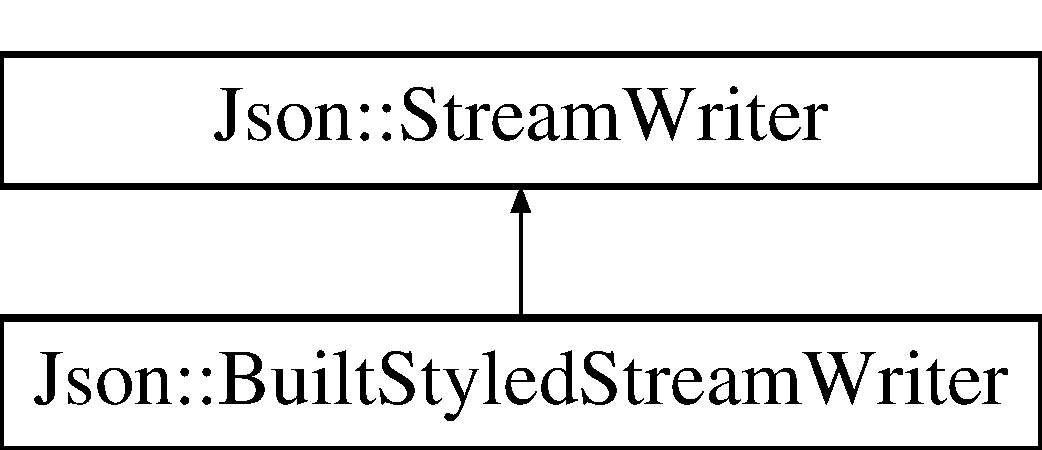
\includegraphics[height=2.000000cm]{classJson_1_1StreamWriter}
\end{center}
\end{figure}
\subsection*{Classes}
\begin{DoxyCompactItemize}
\item 
class \hyperlink{classJson_1_1StreamWriter_1_1Factory}{Factory}
\begin{DoxyCompactList}\small\item\em A simple abstract factory. \end{DoxyCompactList}\end{DoxyCompactItemize}
\subsection*{Public Member Functions}
\begin{DoxyCompactItemize}
\item 
\hyperlink{classJson_1_1StreamWriter_a66e6f5113618ce6b04cac9b3c85a3707}{Stream\+Writer} ()
\item 
virtual \hyperlink{classJson_1_1StreamWriter_a03f8fb6a873b6b50f05bc4556e043c3a}{$\sim$\+Stream\+Writer} ()
\item 
virtual int \hyperlink{classJson_1_1StreamWriter_a84278bad0c9a9fc587bc2a97c5bb5993}{write} (\hyperlink{classJson_1_1Value}{Value} const \&root, \hyperlink{json_8hpp_a37a25be5fca174927780caeb280094ce}{J\+S\+O\+N\+C\+P\+P\+\_\+\+O\+S\+T\+R\+E\+AM} $\ast$sout)=0
\begin{DoxyCompactList}\small\item\em Write \hyperlink{classJson_1_1Value}{Value} into document as configured in sub-\/class. \end{DoxyCompactList}\end{DoxyCompactItemize}
\subsection*{Protected Attributes}
\begin{DoxyCompactItemize}
\item 
\hyperlink{json_8hpp_a37a25be5fca174927780caeb280094ce}{J\+S\+O\+N\+C\+P\+P\+\_\+\+O\+S\+T\+R\+E\+AM} $\ast$ \hyperlink{classJson_1_1StreamWriter_a4f5603d4228a9fa46a42cb44e5234d9b}{sout\+\_\+}
\end{DoxyCompactItemize}


\subsection{Detailed Description}
Usage\+: 


\begin{DoxyCode}
\textcolor{keyword}{using namespace }\hyperlink{namespaceJson}{Json};
\textcolor{keywordtype}{void} writeToStdout(\hyperlink{classJson_1_1StreamWriter_1_1Factory}{StreamWriter::Factory} \textcolor{keyword}{const}& factory, 
      \hyperlink{classJson_1_1Value}{Value} \textcolor{keyword}{const}& value) \{
  std::unique\_ptr<StreamWriter> \textcolor{keyword}{const} writer(
    factory.\hyperlink{classJson_1_1StreamWriter_1_1Factory_a9d30ec53e8288cd53befccf1009c5f31}{newStreamWriter}());
  writer->write(value, &std::cout);
  std::cout << std::endl;  \textcolor{comment}{// add lf and flush}
\}
\end{DoxyCode}
 

\subsection{Constructor \& Destructor Documentation}
\index{Json\+::\+Stream\+Writer@{Json\+::\+Stream\+Writer}!Stream\+Writer@{Stream\+Writer}}
\index{Stream\+Writer@{Stream\+Writer}!Json\+::\+Stream\+Writer@{Json\+::\+Stream\+Writer}}
\subsubsection[{\texorpdfstring{Stream\+Writer()}{StreamWriter()}}]{\setlength{\rightskip}{0pt plus 5cm}Json\+::\+Stream\+Writer\+::\+Stream\+Writer (
\begin{DoxyParamCaption}
{}
\end{DoxyParamCaption}
)}\hypertarget{classJson_1_1StreamWriter_a66e6f5113618ce6b04cac9b3c85a3707}{}\label{classJson_1_1StreamWriter_a66e6f5113618ce6b04cac9b3c85a3707}
\index{Json\+::\+Stream\+Writer@{Json\+::\+Stream\+Writer}!````~Stream\+Writer@{$\sim$\+Stream\+Writer}}
\index{````~Stream\+Writer@{$\sim$\+Stream\+Writer}!Json\+::\+Stream\+Writer@{Json\+::\+Stream\+Writer}}
\subsubsection[{\texorpdfstring{$\sim$\+Stream\+Writer()}{~StreamWriter()}}]{\setlength{\rightskip}{0pt plus 5cm}Json\+::\+Stream\+Writer\+::$\sim$\+Stream\+Writer (
\begin{DoxyParamCaption}
{}
\end{DoxyParamCaption}
)\hspace{0.3cm}{\ttfamily [virtual]}}\hypertarget{classJson_1_1StreamWriter_a03f8fb6a873b6b50f05bc4556e043c3a}{}\label{classJson_1_1StreamWriter_a03f8fb6a873b6b50f05bc4556e043c3a}


\subsection{Member Function Documentation}
\index{Json\+::\+Stream\+Writer@{Json\+::\+Stream\+Writer}!write@{write}}
\index{write@{write}!Json\+::\+Stream\+Writer@{Json\+::\+Stream\+Writer}}
\subsubsection[{\texorpdfstring{write(\+Value const \&root, J\+S\+O\+N\+C\+P\+P\+\_\+\+O\+S\+T\+R\+E\+A\+M $\ast$sout)=0}{write(Value const &root, JSONCPP_OSTREAM *sout)=0}}]{\setlength{\rightskip}{0pt plus 5cm}virtual int Json\+::\+Stream\+Writer\+::write (
\begin{DoxyParamCaption}
\item[{{\bf Value} const \&}]{root, }
\item[{{\bf J\+S\+O\+N\+C\+P\+P\+\_\+\+O\+S\+T\+R\+E\+AM} $\ast$}]{sout}
\end{DoxyParamCaption}
)\hspace{0.3cm}{\ttfamily [pure virtual]}}\hypertarget{classJson_1_1StreamWriter_a84278bad0c9a9fc587bc2a97c5bb5993}{}\label{classJson_1_1StreamWriter_a84278bad0c9a9fc587bc2a97c5bb5993}


Write \hyperlink{classJson_1_1Value}{Value} into document as configured in sub-\/class. 

Do not take ownership of sout, but maintain a reference during function. \begin{DoxyPrecond}{Precondition}
sout != N\+U\+LL 
\end{DoxyPrecond}
\begin{DoxyReturn}{Returns}
zero on success (For now, we always return zero, so check the stream instead.) 
\end{DoxyReturn}

\begin{DoxyExceptions}{Exceptions}
{\em std\+::exception} & possibly, depending on configuration \\
\hline
\end{DoxyExceptions}


Implemented in \hyperlink{structJson_1_1BuiltStyledStreamWriter_a823cdb1afabb6b0d5f39bcd5a6a6f747}{Json\+::\+Built\+Styled\+Stream\+Writer}.



\subsection{Member Data Documentation}
\index{Json\+::\+Stream\+Writer@{Json\+::\+Stream\+Writer}!sout\+\_\+@{sout\+\_\+}}
\index{sout\+\_\+@{sout\+\_\+}!Json\+::\+Stream\+Writer@{Json\+::\+Stream\+Writer}}
\subsubsection[{\texorpdfstring{sout\+\_\+}{sout_}}]{\setlength{\rightskip}{0pt plus 5cm}{\bf J\+S\+O\+N\+C\+P\+P\+\_\+\+O\+S\+T\+R\+E\+AM}$\ast$ Json\+::\+Stream\+Writer\+::sout\+\_\+\hspace{0.3cm}{\ttfamily [protected]}}\hypertarget{classJson_1_1StreamWriter_a4f5603d4228a9fa46a42cb44e5234d9b}{}\label{classJson_1_1StreamWriter_a4f5603d4228a9fa46a42cb44e5234d9b}


The documentation for this class was generated from the following files\+:\begin{DoxyCompactItemize}
\item 
/home/pranav/\+Repositories/zcm/include/\hyperlink{json_8hpp}{json.\+hpp}\item 
/home/pranav/\+Repositories/zcm/src/\hyperlink{json_8cpp}{json.\+cpp}\end{DoxyCompactItemize}

\hypertarget{classJson_1_1StreamWriterBuilder}{}\section{Json\+:\+:Stream\+Writer\+Builder Class Reference}
\label{classJson_1_1StreamWriterBuilder}\index{Json\+::\+Stream\+Writer\+Builder@{Json\+::\+Stream\+Writer\+Builder}}


Build a \hyperlink{classJson_1_1StreamWriter}{Stream\+Writer} implementation.  




{\ttfamily \#include $<$json.\+hpp$>$}

Inheritance diagram for Json\+:\+:Stream\+Writer\+Builder\+:\begin{figure}[H]
\begin{center}
\leavevmode
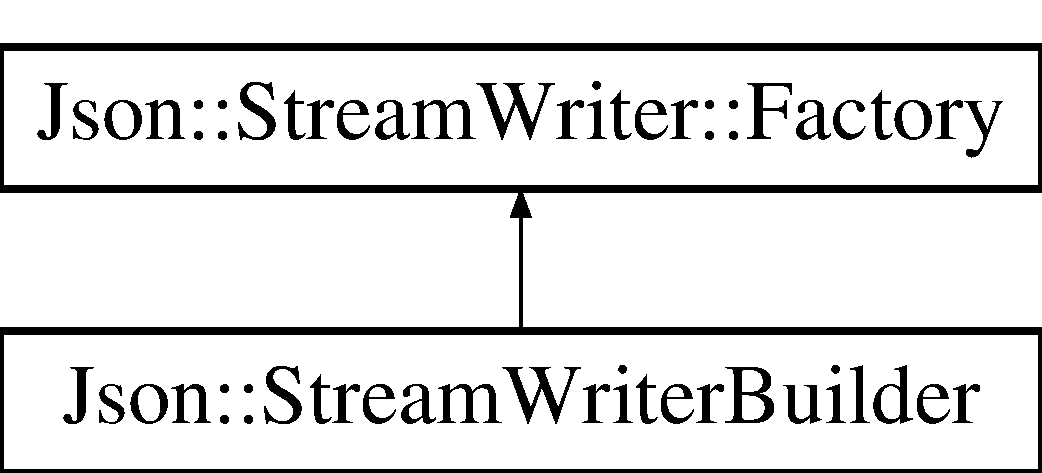
\includegraphics[height=2.000000cm]{classJson_1_1StreamWriterBuilder}
\end{center}
\end{figure}
\subsection*{Public Member Functions}
\begin{DoxyCompactItemize}
\item 
\hyperlink{classJson_1_1StreamWriterBuilder_ab95b76179c152673ad14abc639a46ee4}{Stream\+Writer\+Builder} ()
\item 
\hyperlink{classJson_1_1StreamWriterBuilder_a93263f8ef1e2d22593907075d8f0aaef}{$\sim$\+Stream\+Writer\+Builder} () \hyperlink{json_8hpp_a824d6199c91488107e443226fa6022c5}{J\+S\+O\+N\+C\+P\+P\+\_\+\+O\+V\+E\+R\+R\+I\+DE}
\item 
\hyperlink{classJson_1_1StreamWriter}{Stream\+Writer} $\ast$ \hyperlink{classJson_1_1StreamWriterBuilder_ab9ee278609f88ae04a7c1a84e1f559e6}{new\+Stream\+Writer} () const \hyperlink{json_8hpp_a824d6199c91488107e443226fa6022c5}{J\+S\+O\+N\+C\+P\+P\+\_\+\+O\+V\+E\+R\+R\+I\+DE}
\item 
bool \hyperlink{classJson_1_1StreamWriterBuilder_aa1dfed085a3d369e953e4a3c34da009e}{validate} (\hyperlink{classJson_1_1Value}{Json\+::\+Value} $\ast$invalid) const 
\item 
\hyperlink{classJson_1_1Value}{Value} \& \hyperlink{classJson_1_1StreamWriterBuilder_af68f6b59cb20b074052ed12bb3d336a3}{operator\mbox{[}$\,$\mbox{]}} (\hyperlink{json_8hpp_a1e723f95759de062585bc4a8fd3fa4be}{J\+S\+O\+N\+C\+P\+P\+\_\+\+S\+T\+R\+I\+NG} key)
\begin{DoxyCompactList}\small\item\em A simple way to update a specific setting. \end{DoxyCompactList}\end{DoxyCompactItemize}
\subsection*{Static Public Member Functions}
\begin{DoxyCompactItemize}
\item 
static void \hyperlink{classJson_1_1StreamWriterBuilder_a53bf106b141e28637b01ad0ecd2acbf6}{set\+Defaults} (\hyperlink{classJson_1_1Value}{Json\+::\+Value} $\ast$settings)
\begin{DoxyCompactList}\small\item\em Called by ctor, but you can use this to reset settings\+\_\+. \end{DoxyCompactList}\end{DoxyCompactItemize}
\subsection*{Public Attributes}
\begin{DoxyCompactItemize}
\item 
\hyperlink{classJson_1_1Value}{Json\+::\+Value} \hyperlink{classJson_1_1StreamWriterBuilder_a79bdf2e639a52f4e758c0b95bd1d3423}{settings\+\_\+}
\begin{DoxyCompactList}\small\item\em Configuration of this builder. \end{DoxyCompactList}\end{DoxyCompactItemize}


\subsection{Detailed Description}
Build a \hyperlink{classJson_1_1StreamWriter}{Stream\+Writer} implementation. 

Usage\+: 
\begin{DoxyCode}
\textcolor{keyword}{using namespace }\hyperlink{namespaceJson}{Json};
\hyperlink{classJson_1_1Value}{Value} value = ...;
\hyperlink{classJson_1_1StreamWriterBuilder}{StreamWriterBuilder} builder;
builder[\textcolor{stringliteral}{"commentStyle"}] = \textcolor{stringliteral}{"None"};
builder[\textcolor{stringliteral}{"indentation"}] = \textcolor{stringliteral}{"   "};  \textcolor{comment}{// or whatever you like}
std::unique\_ptr<Json::StreamWriter> writer(
    builder.\hyperlink{classJson_1_1StreamWriterBuilder_ab9ee278609f88ae04a7c1a84e1f559e6}{newStreamWriter}());
writer->write(value, &std::cout);
std::cout << std::endl;  \textcolor{comment}{// add lf and flush}
\end{DoxyCode}
 

\subsection{Constructor \& Destructor Documentation}
\index{Json\+::\+Stream\+Writer\+Builder@{Json\+::\+Stream\+Writer\+Builder}!Stream\+Writer\+Builder@{Stream\+Writer\+Builder}}
\index{Stream\+Writer\+Builder@{Stream\+Writer\+Builder}!Json\+::\+Stream\+Writer\+Builder@{Json\+::\+Stream\+Writer\+Builder}}
\subsubsection[{\texorpdfstring{Stream\+Writer\+Builder()}{StreamWriterBuilder()}}]{\setlength{\rightskip}{0pt plus 5cm}Json\+::\+Stream\+Writer\+Builder\+::\+Stream\+Writer\+Builder (
\begin{DoxyParamCaption}
{}
\end{DoxyParamCaption}
)}\hypertarget{classJson_1_1StreamWriterBuilder_ab95b76179c152673ad14abc639a46ee4}{}\label{classJson_1_1StreamWriterBuilder_ab95b76179c152673ad14abc639a46ee4}
\index{Json\+::\+Stream\+Writer\+Builder@{Json\+::\+Stream\+Writer\+Builder}!````~Stream\+Writer\+Builder@{$\sim$\+Stream\+Writer\+Builder}}
\index{````~Stream\+Writer\+Builder@{$\sim$\+Stream\+Writer\+Builder}!Json\+::\+Stream\+Writer\+Builder@{Json\+::\+Stream\+Writer\+Builder}}
\subsubsection[{\texorpdfstring{$\sim$\+Stream\+Writer\+Builder() J\+S\+O\+N\+C\+P\+P\+\_\+\+O\+V\+E\+R\+R\+I\+DE}{~StreamWriterBuilder() JSONCPP_OVERRIDE}}]{\setlength{\rightskip}{0pt plus 5cm}Json\+::\+Stream\+Writer\+Builder\+::$\sim$\+Stream\+Writer\+Builder (
\begin{DoxyParamCaption}
{}
\end{DoxyParamCaption}
)}\hypertarget{classJson_1_1StreamWriterBuilder_a93263f8ef1e2d22593907075d8f0aaef}{}\label{classJson_1_1StreamWriterBuilder_a93263f8ef1e2d22593907075d8f0aaef}


\subsection{Member Function Documentation}
\index{Json\+::\+Stream\+Writer\+Builder@{Json\+::\+Stream\+Writer\+Builder}!new\+Stream\+Writer@{new\+Stream\+Writer}}
\index{new\+Stream\+Writer@{new\+Stream\+Writer}!Json\+::\+Stream\+Writer\+Builder@{Json\+::\+Stream\+Writer\+Builder}}
\subsubsection[{\texorpdfstring{new\+Stream\+Writer() const J\+S\+O\+N\+C\+P\+P\+\_\+\+O\+V\+E\+R\+R\+I\+DE}{newStreamWriter() const JSONCPP_OVERRIDE}}]{\setlength{\rightskip}{0pt plus 5cm}{\bf Stream\+Writer} $\ast$ Json\+::\+Stream\+Writer\+Builder\+::new\+Stream\+Writer (
\begin{DoxyParamCaption}
{}
\end{DoxyParamCaption}
) const\hspace{0.3cm}{\ttfamily [virtual]}}\hypertarget{classJson_1_1StreamWriterBuilder_ab9ee278609f88ae04a7c1a84e1f559e6}{}\label{classJson_1_1StreamWriterBuilder_ab9ee278609f88ae04a7c1a84e1f559e6}

\begin{DoxyExceptions}{Exceptions}
{\em std\+::exception} & if something goes wrong (e.\+g. invalid settings) \\
\hline
\end{DoxyExceptions}


Implements \hyperlink{classJson_1_1StreamWriter_1_1Factory_a9d30ec53e8288cd53befccf1009c5f31}{Json\+::\+Stream\+Writer\+::\+Factory}.

\index{Json\+::\+Stream\+Writer\+Builder@{Json\+::\+Stream\+Writer\+Builder}!operator\mbox{[}$\,$\mbox{]}@{operator[]}}
\index{operator\mbox{[}$\,$\mbox{]}@{operator[]}!Json\+::\+Stream\+Writer\+Builder@{Json\+::\+Stream\+Writer\+Builder}}
\subsubsection[{\texorpdfstring{operator[](\+J\+S\+O\+N\+C\+P\+P\+\_\+\+S\+T\+R\+I\+N\+G key)}{operator[](JSONCPP_STRING key)}}]{\setlength{\rightskip}{0pt plus 5cm}{\bf Value} \& Json\+::\+Stream\+Writer\+Builder\+::operator\mbox{[}$\,$\mbox{]} (
\begin{DoxyParamCaption}
\item[{{\bf J\+S\+O\+N\+C\+P\+P\+\_\+\+S\+T\+R\+I\+NG}}]{key}
\end{DoxyParamCaption}
)}\hypertarget{classJson_1_1StreamWriterBuilder_af68f6b59cb20b074052ed12bb3d336a3}{}\label{classJson_1_1StreamWriterBuilder_af68f6b59cb20b074052ed12bb3d336a3}


A simple way to update a specific setting. 

\index{Json\+::\+Stream\+Writer\+Builder@{Json\+::\+Stream\+Writer\+Builder}!set\+Defaults@{set\+Defaults}}
\index{set\+Defaults@{set\+Defaults}!Json\+::\+Stream\+Writer\+Builder@{Json\+::\+Stream\+Writer\+Builder}}
\subsubsection[{\texorpdfstring{set\+Defaults(\+Json\+::\+Value $\ast$settings)}{setDefaults(Json::Value *settings)}}]{\setlength{\rightskip}{0pt plus 5cm}void Json\+::\+Stream\+Writer\+Builder\+::set\+Defaults (
\begin{DoxyParamCaption}
\item[{{\bf Json\+::\+Value} $\ast$}]{settings}
\end{DoxyParamCaption}
)\hspace{0.3cm}{\ttfamily [static]}}\hypertarget{classJson_1_1StreamWriterBuilder_a53bf106b141e28637b01ad0ecd2acbf6}{}\label{classJson_1_1StreamWriterBuilder_a53bf106b141e28637b01ad0ecd2acbf6}


Called by ctor, but you can use this to reset settings\+\_\+. 

\begin{DoxyPrecond}{Precondition}
\textquotesingle{}settings\textquotesingle{} != N\+U\+LL (but Json\+::null is fine) 
\end{DoxyPrecond}
\begin{DoxyRemark}{Remarks}
Defaults\+: 
\begin{DoxyCodeInclude}
\end{DoxyCodeInclude}

\end{DoxyRemark}
\mbox{[}Stream\+Writer\+Builder\+Defaults\mbox{]}

\mbox{[}Stream\+Writer\+Builder\+Defaults\mbox{]} \index{Json\+::\+Stream\+Writer\+Builder@{Json\+::\+Stream\+Writer\+Builder}!validate@{validate}}
\index{validate@{validate}!Json\+::\+Stream\+Writer\+Builder@{Json\+::\+Stream\+Writer\+Builder}}
\subsubsection[{\texorpdfstring{validate(\+Json\+::\+Value $\ast$invalid) const }{validate(Json::Value *invalid) const }}]{\setlength{\rightskip}{0pt plus 5cm}bool Json\+::\+Stream\+Writer\+Builder\+::validate (
\begin{DoxyParamCaption}
\item[{{\bf Json\+::\+Value} $\ast$}]{invalid}
\end{DoxyParamCaption}
) const}\hypertarget{classJson_1_1StreamWriterBuilder_aa1dfed085a3d369e953e4a3c34da009e}{}\label{classJson_1_1StreamWriterBuilder_aa1dfed085a3d369e953e4a3c34da009e}
\begin{DoxyReturn}{Returns}
true if \textquotesingle{}settings\textquotesingle{} are legal and consistent; otherwise, indicate bad settings via \textquotesingle{}invalid\textquotesingle{}. 
\end{DoxyReturn}


\subsection{Member Data Documentation}
\index{Json\+::\+Stream\+Writer\+Builder@{Json\+::\+Stream\+Writer\+Builder}!settings\+\_\+@{settings\+\_\+}}
\index{settings\+\_\+@{settings\+\_\+}!Json\+::\+Stream\+Writer\+Builder@{Json\+::\+Stream\+Writer\+Builder}}
\subsubsection[{\texorpdfstring{settings\+\_\+}{settings_}}]{\setlength{\rightskip}{0pt plus 5cm}{\bf Json\+::\+Value} Json\+::\+Stream\+Writer\+Builder\+::settings\+\_\+}\hypertarget{classJson_1_1StreamWriterBuilder_a79bdf2e639a52f4e758c0b95bd1d3423}{}\label{classJson_1_1StreamWriterBuilder_a79bdf2e639a52f4e758c0b95bd1d3423}


Configuration of this builder. 

Available settings (case-\/sensitive)\+:
\begin{DoxyItemize}
\item \char`\"{}comment\+Style\char`\"{}\+: \char`\"{}\+None\char`\"{} or \char`\"{}\+All\char`\"{}
\item \char`\"{}indentation\char`\"{}\+: \char`\"{}$<$anything$>$\char`\"{}
\item \char`\"{}enable\+Y\+A\+M\+L\+Compatibility\char`\"{}\+: false or true
\begin{DoxyItemize}
\item slightly change the whitespace around colons
\end{DoxyItemize}
\item \char`\"{}drop\+Null\+Placeholders\char`\"{}\+: false or true
\begin{DoxyItemize}
\item Drop the \char`\"{}null\char`\"{} string from the writer\textquotesingle{}s output for null\+Values. Strictly speaking, this is not valid J\+S\+ON. But when the output is being fed to a browser\textquotesingle{}s Javascript, it makes for smaller output and the browser can handle the output just fine.
\end{DoxyItemize}
\item \char`\"{}use\+Special\+Floats\char`\"{}\+: false or true
\begin{DoxyItemize}
\item If true, outputs non-\/finite floating point values in the following way\+: NaN values as \char`\"{}\+Na\+N\char`\"{}, positive infinity as \char`\"{}\+Infinity\char`\"{}, and negative infinity as \char`\"{}-\/\+Infinity\char`\"{}.
\end{DoxyItemize}
\end{DoxyItemize}

You can examine \textquotesingle{}settings\+\_\+` yourself to see the defaults. You can also write and read them just like any J\+S\+ON \hyperlink{classJson_1_1Value}{Value}. \begin{DoxySeeAlso}{See also}
\hyperlink{classJson_1_1StreamWriterBuilder_a53bf106b141e28637b01ad0ecd2acbf6}{set\+Defaults()} 
\end{DoxySeeAlso}


The documentation for this class was generated from the following files\+:\begin{DoxyCompactItemize}
\item 
/home/pranav/\+Repositories/zcm/include/\hyperlink{json_8hpp}{json.\+hpp}\item 
/home/pranav/\+Repositories/zcm/src/\hyperlink{json_8cpp}{json.\+cpp}\end{DoxyCompactItemize}

\hypertarget{structJson_1_1Value_1_1CZString_1_1StringStorage}{}\section{Json\+:\+:Value\+:\+:C\+Z\+String\+:\+:String\+Storage Struct Reference}
\label{structJson_1_1Value_1_1CZString_1_1StringStorage}\index{Json\+::\+Value\+::\+C\+Z\+String\+::\+String\+Storage@{Json\+::\+Value\+::\+C\+Z\+String\+::\+String\+Storage}}
\subsection*{Public Attributes}
\begin{DoxyCompactItemize}
\item 
unsigned \hyperlink{structJson_1_1Value_1_1CZString_1_1StringStorage_a7f68c8d6197c5692a525854b5f29f87b}{policy\+\_\+}\+: 2
\item 
unsigned \hyperlink{structJson_1_1Value_1_1CZString_1_1StringStorage_a165d865c44e6471d34668eeb4f15b140}{length\+\_\+}\+: 30
\end{DoxyCompactItemize}


\subsection{Member Data Documentation}
\index{Json\+::\+Value\+::\+C\+Z\+String\+::\+String\+Storage@{Json\+::\+Value\+::\+C\+Z\+String\+::\+String\+Storage}!length\+\_\+@{length\+\_\+}}
\index{length\+\_\+@{length\+\_\+}!Json\+::\+Value\+::\+C\+Z\+String\+::\+String\+Storage@{Json\+::\+Value\+::\+C\+Z\+String\+::\+String\+Storage}}
\subsubsection[{\texorpdfstring{length\+\_\+}{length_}}]{\setlength{\rightskip}{0pt plus 5cm}unsigned Json\+::\+Value\+::\+C\+Z\+String\+::\+String\+Storage\+::length\+\_\+}\hypertarget{structJson_1_1Value_1_1CZString_1_1StringStorage_a165d865c44e6471d34668eeb4f15b140}{}\label{structJson_1_1Value_1_1CZString_1_1StringStorage_a165d865c44e6471d34668eeb4f15b140}
\index{Json\+::\+Value\+::\+C\+Z\+String\+::\+String\+Storage@{Json\+::\+Value\+::\+C\+Z\+String\+::\+String\+Storage}!policy\+\_\+@{policy\+\_\+}}
\index{policy\+\_\+@{policy\+\_\+}!Json\+::\+Value\+::\+C\+Z\+String\+::\+String\+Storage@{Json\+::\+Value\+::\+C\+Z\+String\+::\+String\+Storage}}
\subsubsection[{\texorpdfstring{policy\+\_\+}{policy_}}]{\setlength{\rightskip}{0pt plus 5cm}unsigned Json\+::\+Value\+::\+C\+Z\+String\+::\+String\+Storage\+::policy\+\_\+}\hypertarget{structJson_1_1Value_1_1CZString_1_1StringStorage_a7f68c8d6197c5692a525854b5f29f87b}{}\label{structJson_1_1Value_1_1CZString_1_1StringStorage_a7f68c8d6197c5692a525854b5f29f87b}


The documentation for this struct was generated from the following file\+:\begin{DoxyCompactItemize}
\item 
/home/pranav/\+Repositories/zcm/include/\hyperlink{json_8hpp}{json.\+hpp}\end{DoxyCompactItemize}

\hypertarget{structJson_1_1Reader_1_1StructuredError}{}\section{Json\+:\+:Reader\+:\+:Structured\+Error Struct Reference}
\label{structJson_1_1Reader_1_1StructuredError}\index{Json\+::\+Reader\+::\+Structured\+Error@{Json\+::\+Reader\+::\+Structured\+Error}}


An error tagged with where in the J\+S\+ON text it was encountered.  




{\ttfamily \#include $<$json.\+hpp$>$}

\subsection*{Public Attributes}
\begin{DoxyCompactItemize}
\item 
ptrdiff\+\_\+t \hyperlink{structJson_1_1Reader_1_1StructuredError_ac98af0da2d704be4b64a9572a682423b}{offset\+\_\+start}
\item 
ptrdiff\+\_\+t \hyperlink{structJson_1_1Reader_1_1StructuredError_ad76ac01aeb0ada7e882c2df5daa54c6e}{offset\+\_\+limit}
\item 
\hyperlink{json_8hpp_a1e723f95759de062585bc4a8fd3fa4be}{J\+S\+O\+N\+C\+P\+P\+\_\+\+S\+T\+R\+I\+NG} \hyperlink{structJson_1_1Reader_1_1StructuredError_a2d2dc387aefe406a71de3daa263a38f4}{message}
\end{DoxyCompactItemize}


\subsection{Detailed Description}
An error tagged with where in the J\+S\+ON text it was encountered. 

The offsets give the \mbox{[}start, limit) range of bytes within the text. Note that this is bytes, not codepoints. 

\subsection{Member Data Documentation}
\index{Json\+::\+Reader\+::\+Structured\+Error@{Json\+::\+Reader\+::\+Structured\+Error}!message@{message}}
\index{message@{message}!Json\+::\+Reader\+::\+Structured\+Error@{Json\+::\+Reader\+::\+Structured\+Error}}
\subsubsection[{\texorpdfstring{message}{message}}]{\setlength{\rightskip}{0pt plus 5cm}{\bf J\+S\+O\+N\+C\+P\+P\+\_\+\+S\+T\+R\+I\+NG} Json\+::\+Reader\+::\+Structured\+Error\+::message}\hypertarget{structJson_1_1Reader_1_1StructuredError_a2d2dc387aefe406a71de3daa263a38f4}{}\label{structJson_1_1Reader_1_1StructuredError_a2d2dc387aefe406a71de3daa263a38f4}
\index{Json\+::\+Reader\+::\+Structured\+Error@{Json\+::\+Reader\+::\+Structured\+Error}!offset\+\_\+limit@{offset\+\_\+limit}}
\index{offset\+\_\+limit@{offset\+\_\+limit}!Json\+::\+Reader\+::\+Structured\+Error@{Json\+::\+Reader\+::\+Structured\+Error}}
\subsubsection[{\texorpdfstring{offset\+\_\+limit}{offset_limit}}]{\setlength{\rightskip}{0pt plus 5cm}ptrdiff\+\_\+t Json\+::\+Reader\+::\+Structured\+Error\+::offset\+\_\+limit}\hypertarget{structJson_1_1Reader_1_1StructuredError_ad76ac01aeb0ada7e882c2df5daa54c6e}{}\label{structJson_1_1Reader_1_1StructuredError_ad76ac01aeb0ada7e882c2df5daa54c6e}
\index{Json\+::\+Reader\+::\+Structured\+Error@{Json\+::\+Reader\+::\+Structured\+Error}!offset\+\_\+start@{offset\+\_\+start}}
\index{offset\+\_\+start@{offset\+\_\+start}!Json\+::\+Reader\+::\+Structured\+Error@{Json\+::\+Reader\+::\+Structured\+Error}}
\subsubsection[{\texorpdfstring{offset\+\_\+start}{offset_start}}]{\setlength{\rightskip}{0pt plus 5cm}ptrdiff\+\_\+t Json\+::\+Reader\+::\+Structured\+Error\+::offset\+\_\+start}\hypertarget{structJson_1_1Reader_1_1StructuredError_ac98af0da2d704be4b64a9572a682423b}{}\label{structJson_1_1Reader_1_1StructuredError_ac98af0da2d704be4b64a9572a682423b}


The documentation for this struct was generated from the following file\+:\begin{DoxyCompactItemize}
\item 
/home/pranav/\+Repositories/zcm/include/\hyperlink{json_8hpp}{json.\+hpp}\end{DoxyCompactItemize}

\hypertarget{structJson_1_1OurReader_1_1StructuredError}{}\section{Json\+:\+:Our\+Reader\+:\+:Structured\+Error Struct Reference}
\label{structJson_1_1OurReader_1_1StructuredError}\index{Json\+::\+Our\+Reader\+::\+Structured\+Error@{Json\+::\+Our\+Reader\+::\+Structured\+Error}}
\subsection*{Public Attributes}
\begin{DoxyCompactItemize}
\item 
ptrdiff\+\_\+t \hyperlink{structJson_1_1OurReader_1_1StructuredError_a102677698afb8177c985e72dafe72b15}{offset\+\_\+start}
\item 
ptrdiff\+\_\+t \hyperlink{structJson_1_1OurReader_1_1StructuredError_a15491a751a39c5153af04e68b1d0abb9}{offset\+\_\+limit}
\item 
\hyperlink{json_8hpp_a1e723f95759de062585bc4a8fd3fa4be}{J\+S\+O\+N\+C\+P\+P\+\_\+\+S\+T\+R\+I\+NG} \hyperlink{structJson_1_1OurReader_1_1StructuredError_a9d0b9986bf765d067dfcf2f971a450d1}{message}
\end{DoxyCompactItemize}


\subsection{Member Data Documentation}
\index{Json\+::\+Our\+Reader\+::\+Structured\+Error@{Json\+::\+Our\+Reader\+::\+Structured\+Error}!message@{message}}
\index{message@{message}!Json\+::\+Our\+Reader\+::\+Structured\+Error@{Json\+::\+Our\+Reader\+::\+Structured\+Error}}
\subsubsection[{\texorpdfstring{message}{message}}]{\setlength{\rightskip}{0pt plus 5cm}{\bf J\+S\+O\+N\+C\+P\+P\+\_\+\+S\+T\+R\+I\+NG} Json\+::\+Our\+Reader\+::\+Structured\+Error\+::message}\hypertarget{structJson_1_1OurReader_1_1StructuredError_a9d0b9986bf765d067dfcf2f971a450d1}{}\label{structJson_1_1OurReader_1_1StructuredError_a9d0b9986bf765d067dfcf2f971a450d1}
\index{Json\+::\+Our\+Reader\+::\+Structured\+Error@{Json\+::\+Our\+Reader\+::\+Structured\+Error}!offset\+\_\+limit@{offset\+\_\+limit}}
\index{offset\+\_\+limit@{offset\+\_\+limit}!Json\+::\+Our\+Reader\+::\+Structured\+Error@{Json\+::\+Our\+Reader\+::\+Structured\+Error}}
\subsubsection[{\texorpdfstring{offset\+\_\+limit}{offset_limit}}]{\setlength{\rightskip}{0pt plus 5cm}ptrdiff\+\_\+t Json\+::\+Our\+Reader\+::\+Structured\+Error\+::offset\+\_\+limit}\hypertarget{structJson_1_1OurReader_1_1StructuredError_a15491a751a39c5153af04e68b1d0abb9}{}\label{structJson_1_1OurReader_1_1StructuredError_a15491a751a39c5153af04e68b1d0abb9}
\index{Json\+::\+Our\+Reader\+::\+Structured\+Error@{Json\+::\+Our\+Reader\+::\+Structured\+Error}!offset\+\_\+start@{offset\+\_\+start}}
\index{offset\+\_\+start@{offset\+\_\+start}!Json\+::\+Our\+Reader\+::\+Structured\+Error@{Json\+::\+Our\+Reader\+::\+Structured\+Error}}
\subsubsection[{\texorpdfstring{offset\+\_\+start}{offset_start}}]{\setlength{\rightskip}{0pt plus 5cm}ptrdiff\+\_\+t Json\+::\+Our\+Reader\+::\+Structured\+Error\+::offset\+\_\+start}\hypertarget{structJson_1_1OurReader_1_1StructuredError_a102677698afb8177c985e72dafe72b15}{}\label{structJson_1_1OurReader_1_1StructuredError_a102677698afb8177c985e72dafe72b15}


The documentation for this struct was generated from the following file\+:\begin{DoxyCompactItemize}
\item 
/home/pranav/\+Repositories/zcm/src/\hyperlink{json_8cpp}{json.\+cpp}\end{DoxyCompactItemize}

\hypertarget{classJson_1_1StyledStreamWriter}{}\section{Json\+:\+:Styled\+Stream\+Writer Class Reference}
\label{classJson_1_1StyledStreamWriter}\index{Json\+::\+Styled\+Stream\+Writer@{Json\+::\+Styled\+Stream\+Writer}}


Writes a \hyperlink{classJson_1_1Value}{Value} in \href{http://www.json.org}{\tt J\+S\+ON} format in a human friendly way, to a stream rather than to a string.  




{\ttfamily \#include $<$json.\+hpp$>$}

\subsection*{Public Member Functions}
\begin{DoxyCompactItemize}
\item 
\hyperlink{classJson_1_1StyledStreamWriter_a71fe3b45a3a5fd6616d807ca99d1a1ef}{Styled\+Stream\+Writer} (\hyperlink{json_8hpp_a1e723f95759de062585bc4a8fd3fa4be}{J\+S\+O\+N\+C\+P\+P\+\_\+\+S\+T\+R\+I\+NG} indentation=\char`\"{}\textbackslash{}t\char`\"{})
\item 
\hyperlink{classJson_1_1StyledStreamWriter_a17444a59f617970279714e97b0ddfa46}{$\sim$\+Styled\+Stream\+Writer} ()
\item 
void \hyperlink{classJson_1_1StyledStreamWriter_a5d89d984fe675641e42c4370cd247774}{write} (\hyperlink{json_8hpp_a37a25be5fca174927780caeb280094ce}{J\+S\+O\+N\+C\+P\+P\+\_\+\+O\+S\+T\+R\+E\+AM} \&out, const \hyperlink{classJson_1_1Value}{Value} \&root)
\begin{DoxyCompactList}\small\item\em Serialize a \hyperlink{classJson_1_1Value}{Value} in \href{http://www.json.org}{\tt J\+S\+ON} format. \end{DoxyCompactList}\end{DoxyCompactItemize}
\subsection*{Private Types}
\begin{DoxyCompactItemize}
\item 
typedef std\+::vector$<$ \hyperlink{json_8hpp_a1e723f95759de062585bc4a8fd3fa4be}{J\+S\+O\+N\+C\+P\+P\+\_\+\+S\+T\+R\+I\+NG} $>$ \hyperlink{classJson_1_1StyledStreamWriter_a259bf9d99847b2ea64ec9c6dd441944e}{Child\+Values}
\end{DoxyCompactItemize}
\subsection*{Private Member Functions}
\begin{DoxyCompactItemize}
\item 
void \hyperlink{classJson_1_1StyledStreamWriter_a4359250e09273fa0144021684be001ae}{write\+Value} (const \hyperlink{classJson_1_1Value}{Value} \&value)
\item 
void \hyperlink{classJson_1_1StyledStreamWriter_a606f2ddd58093c9b019d452c1b6f09fe}{write\+Array\+Value} (const \hyperlink{classJson_1_1Value}{Value} \&value)
\item 
bool \hyperlink{classJson_1_1StyledStreamWriter_a88f4d342cf25c73aabf77c1b8ba01e44}{is\+Multine\+Array} (const \hyperlink{classJson_1_1Value}{Value} \&value)
\item 
void \hyperlink{classJson_1_1StyledStreamWriter_a9adb47185695f07b1979d8f4c5347592}{push\+Value} (const \hyperlink{json_8hpp_a1e723f95759de062585bc4a8fd3fa4be}{J\+S\+O\+N\+C\+P\+P\+\_\+\+S\+T\+R\+I\+NG} \&value)
\item 
void \hyperlink{classJson_1_1StyledStreamWriter_a5a52fa5b406f1580a61dde3b5638e76d}{write\+Indent} ()
\item 
void \hyperlink{classJson_1_1StyledStreamWriter_a4e64789373b359c9b7a7244509b918fc}{write\+With\+Indent} (const \hyperlink{json_8hpp_a1e723f95759de062585bc4a8fd3fa4be}{J\+S\+O\+N\+C\+P\+P\+\_\+\+S\+T\+R\+I\+NG} \&value)
\item 
void \hyperlink{classJson_1_1StyledStreamWriter_ab49409578422aa73b060e3492dd6c72a}{indent} ()
\item 
void \hyperlink{classJson_1_1StyledStreamWriter_a74d8fb9beecd29759d7b79f430386358}{unindent} ()
\item 
void \hyperlink{classJson_1_1StyledStreamWriter_a79c3c2b320475035c47b2db484a3e434}{write\+Comment\+Before\+Value} (const \hyperlink{classJson_1_1Value}{Value} \&root)
\item 
void \hyperlink{classJson_1_1StyledStreamWriter_ad2ca860e317ca91d6b2932535b4ce9c7}{write\+Comment\+After\+Value\+On\+Same\+Line} (const \hyperlink{classJson_1_1Value}{Value} \&root)
\item 
bool \hyperlink{classJson_1_1StyledStreamWriter_ad2892f57171919fa4f8a5ae5574755cf}{has\+Comment\+For\+Value} (const \hyperlink{classJson_1_1Value}{Value} \&value)
\end{DoxyCompactItemize}
\subsection*{Static Private Member Functions}
\begin{DoxyCompactItemize}
\item 
static \hyperlink{json_8hpp_a1e723f95759de062585bc4a8fd3fa4be}{J\+S\+O\+N\+C\+P\+P\+\_\+\+S\+T\+R\+I\+NG} \hyperlink{classJson_1_1StyledStreamWriter_ae481322d7a439881b257ba7aeda6d19b}{normalize\+E\+OL} (const \hyperlink{json_8hpp_a1e723f95759de062585bc4a8fd3fa4be}{J\+S\+O\+N\+C\+P\+P\+\_\+\+S\+T\+R\+I\+NG} \&text)
\end{DoxyCompactItemize}
\subsection*{Private Attributes}
\begin{DoxyCompactItemize}
\item 
\hyperlink{classJson_1_1StyledStreamWriter_a259bf9d99847b2ea64ec9c6dd441944e}{Child\+Values} \hyperlink{classJson_1_1StyledStreamWriter_aafd62e00a401df73fcacb2e410114b3d}{child\+Values\+\_\+}
\item 
\hyperlink{json_8hpp_a37a25be5fca174927780caeb280094ce}{J\+S\+O\+N\+C\+P\+P\+\_\+\+O\+S\+T\+R\+E\+AM} $\ast$ \hyperlink{classJson_1_1StyledStreamWriter_aa8c4e4576f5c3dcb10955d133a092dd6}{document\+\_\+}
\item 
\hyperlink{json_8hpp_a1e723f95759de062585bc4a8fd3fa4be}{J\+S\+O\+N\+C\+P\+P\+\_\+\+S\+T\+R\+I\+NG} \hyperlink{classJson_1_1StyledStreamWriter_a1481433ebe1491ea83b0beb92aed56c2}{indent\+String\+\_\+}
\item 
unsigned int \hyperlink{classJson_1_1StyledStreamWriter_a94299ec0a9bb925b2dbbab7c1f2b390a}{right\+Margin\+\_\+}
\item 
\hyperlink{json_8hpp_a1e723f95759de062585bc4a8fd3fa4be}{J\+S\+O\+N\+C\+P\+P\+\_\+\+S\+T\+R\+I\+NG} \hyperlink{classJson_1_1StyledStreamWriter_aa45d8fb4ca82d0550be9042012303713}{indentation\+\_\+}
\item 
bool \hyperlink{classJson_1_1StyledStreamWriter_a4e4bb7fc223b2652b72b523b1ce414fa}{add\+Child\+Values\+\_\+}\+: 1
\item 
bool \hyperlink{classJson_1_1StyledStreamWriter_aa12db1753619a9b48da41f3e45e3275d}{indented\+\_\+}\+: 1
\end{DoxyCompactItemize}


\subsection{Detailed Description}
Writes a \hyperlink{classJson_1_1Value}{Value} in \href{http://www.json.org}{\tt J\+S\+ON} format in a human friendly way, to a stream rather than to a string. 

The rules for line break and indent are as follow\+:
\begin{DoxyItemize}
\item Object value\+:
\begin{DoxyItemize}
\item if empty then print \{\} without indent and line break
\item if not empty the print \textquotesingle{}\{\textquotesingle{}, line break \& indent, print one value per line and then unindent and line break and print \textquotesingle{}\}\textquotesingle{}.
\end{DoxyItemize}
\item Array value\+:
\begin{DoxyItemize}
\item if empty then print \mbox{[}\mbox{]} without indent and line break
\item if the array contains no object value, empty array or some other value types, and all the values fit on one lines, then print the array on a single line.
\item otherwise, it the values do not fit on one line, or the array contains object or non empty array, then print one value per line.
\end{DoxyItemize}
\end{DoxyItemize}

If the \hyperlink{classJson_1_1Value}{Value} have comments then they are outputed according to their \hyperlink{namespaceJson_a4fc417c23905b2ae9e2c47d197a45351}{Comment\+Placement}.


\begin{DoxyParams}{Parameters}
{\em indentation} & Each level will be indented by this amount extra. \\
\hline
\end{DoxyParams}
\begin{DoxySeeAlso}{See also}
\hyperlink{classJson_1_1Reader}{Reader}, \hyperlink{classJson_1_1Value}{Value}, \hyperlink{classJson_1_1Value_a29f3a30f7e5d3af6f38d57999bf5b480}{Value\+::set\+Comment()} 
\end{DoxySeeAlso}
\begin{DoxyRefDesc}{Deprecated}
\item[\hyperlink{deprecated__deprecated000010}{Deprecated}]Use \hyperlink{classJson_1_1StreamWriterBuilder}{Stream\+Writer\+Builder}. \end{DoxyRefDesc}


\subsection{Member Typedef Documentation}
\index{Json\+::\+Styled\+Stream\+Writer@{Json\+::\+Styled\+Stream\+Writer}!Child\+Values@{Child\+Values}}
\index{Child\+Values@{Child\+Values}!Json\+::\+Styled\+Stream\+Writer@{Json\+::\+Styled\+Stream\+Writer}}
\subsubsection[{\texorpdfstring{Child\+Values}{ChildValues}}]{\setlength{\rightskip}{0pt plus 5cm}typedef std\+::vector$<${\bf J\+S\+O\+N\+C\+P\+P\+\_\+\+S\+T\+R\+I\+NG}$>$ {\bf Json\+::\+Styled\+Stream\+Writer\+::\+Child\+Values}\hspace{0.3cm}{\ttfamily [private]}}\hypertarget{classJson_1_1StyledStreamWriter_a259bf9d99847b2ea64ec9c6dd441944e}{}\label{classJson_1_1StyledStreamWriter_a259bf9d99847b2ea64ec9c6dd441944e}


\subsection{Constructor \& Destructor Documentation}
\index{Json\+::\+Styled\+Stream\+Writer@{Json\+::\+Styled\+Stream\+Writer}!Styled\+Stream\+Writer@{Styled\+Stream\+Writer}}
\index{Styled\+Stream\+Writer@{Styled\+Stream\+Writer}!Json\+::\+Styled\+Stream\+Writer@{Json\+::\+Styled\+Stream\+Writer}}
\subsubsection[{\texorpdfstring{Styled\+Stream\+Writer(\+J\+S\+O\+N\+C\+P\+P\+\_\+\+S\+T\+R\+I\+N\+G indentation=""\textbackslash{}t"")}{StyledStreamWriter(JSONCPP_STRING indentation="\textbackslash{}t")}}]{\setlength{\rightskip}{0pt plus 5cm}Json\+::\+Styled\+Stream\+Writer\+::\+Styled\+Stream\+Writer (
\begin{DoxyParamCaption}
\item[{{\bf J\+S\+O\+N\+C\+P\+P\+\_\+\+S\+T\+R\+I\+NG}}]{indentation = {\ttfamily \char`\"{}\textbackslash{}t\char`\"{}}}
\end{DoxyParamCaption}
)}\hypertarget{classJson_1_1StyledStreamWriter_a71fe3b45a3a5fd6616d807ca99d1a1ef}{}\label{classJson_1_1StyledStreamWriter_a71fe3b45a3a5fd6616d807ca99d1a1ef}
\index{Json\+::\+Styled\+Stream\+Writer@{Json\+::\+Styled\+Stream\+Writer}!````~Styled\+Stream\+Writer@{$\sim$\+Styled\+Stream\+Writer}}
\index{````~Styled\+Stream\+Writer@{$\sim$\+Styled\+Stream\+Writer}!Json\+::\+Styled\+Stream\+Writer@{Json\+::\+Styled\+Stream\+Writer}}
\subsubsection[{\texorpdfstring{$\sim$\+Styled\+Stream\+Writer()}{~StyledStreamWriter()}}]{\setlength{\rightskip}{0pt plus 5cm}Json\+::\+Styled\+Stream\+Writer\+::$\sim$\+Styled\+Stream\+Writer (
\begin{DoxyParamCaption}
{}
\end{DoxyParamCaption}
)\hspace{0.3cm}{\ttfamily [inline]}}\hypertarget{classJson_1_1StyledStreamWriter_a17444a59f617970279714e97b0ddfa46}{}\label{classJson_1_1StyledStreamWriter_a17444a59f617970279714e97b0ddfa46}


\subsection{Member Function Documentation}
\index{Json\+::\+Styled\+Stream\+Writer@{Json\+::\+Styled\+Stream\+Writer}!has\+Comment\+For\+Value@{has\+Comment\+For\+Value}}
\index{has\+Comment\+For\+Value@{has\+Comment\+For\+Value}!Json\+::\+Styled\+Stream\+Writer@{Json\+::\+Styled\+Stream\+Writer}}
\subsubsection[{\texorpdfstring{has\+Comment\+For\+Value(const Value \&value)}{hasCommentForValue(const Value &value)}}]{\setlength{\rightskip}{0pt plus 5cm}bool Json\+::\+Styled\+Stream\+Writer\+::has\+Comment\+For\+Value (
\begin{DoxyParamCaption}
\item[{const {\bf Value} \&}]{value}
\end{DoxyParamCaption}
)\hspace{0.3cm}{\ttfamily [private]}}\hypertarget{classJson_1_1StyledStreamWriter_ad2892f57171919fa4f8a5ae5574755cf}{}\label{classJson_1_1StyledStreamWriter_ad2892f57171919fa4f8a5ae5574755cf}
\index{Json\+::\+Styled\+Stream\+Writer@{Json\+::\+Styled\+Stream\+Writer}!indent@{indent}}
\index{indent@{indent}!Json\+::\+Styled\+Stream\+Writer@{Json\+::\+Styled\+Stream\+Writer}}
\subsubsection[{\texorpdfstring{indent()}{indent()}}]{\setlength{\rightskip}{0pt plus 5cm}void Json\+::\+Styled\+Stream\+Writer\+::indent (
\begin{DoxyParamCaption}
{}
\end{DoxyParamCaption}
)\hspace{0.3cm}{\ttfamily [private]}}\hypertarget{classJson_1_1StyledStreamWriter_ab49409578422aa73b060e3492dd6c72a}{}\label{classJson_1_1StyledStreamWriter_ab49409578422aa73b060e3492dd6c72a}
\index{Json\+::\+Styled\+Stream\+Writer@{Json\+::\+Styled\+Stream\+Writer}!is\+Multine\+Array@{is\+Multine\+Array}}
\index{is\+Multine\+Array@{is\+Multine\+Array}!Json\+::\+Styled\+Stream\+Writer@{Json\+::\+Styled\+Stream\+Writer}}
\subsubsection[{\texorpdfstring{is\+Multine\+Array(const Value \&value)}{isMultineArray(const Value &value)}}]{\setlength{\rightskip}{0pt plus 5cm}bool Json\+::\+Styled\+Stream\+Writer\+::is\+Multine\+Array (
\begin{DoxyParamCaption}
\item[{const {\bf Value} \&}]{value}
\end{DoxyParamCaption}
)\hspace{0.3cm}{\ttfamily [private]}}\hypertarget{classJson_1_1StyledStreamWriter_a88f4d342cf25c73aabf77c1b8ba01e44}{}\label{classJson_1_1StyledStreamWriter_a88f4d342cf25c73aabf77c1b8ba01e44}
\index{Json\+::\+Styled\+Stream\+Writer@{Json\+::\+Styled\+Stream\+Writer}!normalize\+E\+OL@{normalize\+E\+OL}}
\index{normalize\+E\+OL@{normalize\+E\+OL}!Json\+::\+Styled\+Stream\+Writer@{Json\+::\+Styled\+Stream\+Writer}}
\subsubsection[{\texorpdfstring{normalize\+E\+O\+L(const J\+S\+O\+N\+C\+P\+P\+\_\+\+S\+T\+R\+I\+N\+G \&text)}{normalizeEOL(const JSONCPP_STRING &text)}}]{\setlength{\rightskip}{0pt plus 5cm}static {\bf J\+S\+O\+N\+C\+P\+P\+\_\+\+S\+T\+R\+I\+NG} Json\+::\+Styled\+Stream\+Writer\+::normalize\+E\+OL (
\begin{DoxyParamCaption}
\item[{const {\bf J\+S\+O\+N\+C\+P\+P\+\_\+\+S\+T\+R\+I\+NG} \&}]{text}
\end{DoxyParamCaption}
)\hspace{0.3cm}{\ttfamily [static]}, {\ttfamily [private]}}\hypertarget{classJson_1_1StyledStreamWriter_ae481322d7a439881b257ba7aeda6d19b}{}\label{classJson_1_1StyledStreamWriter_ae481322d7a439881b257ba7aeda6d19b}
\index{Json\+::\+Styled\+Stream\+Writer@{Json\+::\+Styled\+Stream\+Writer}!push\+Value@{push\+Value}}
\index{push\+Value@{push\+Value}!Json\+::\+Styled\+Stream\+Writer@{Json\+::\+Styled\+Stream\+Writer}}
\subsubsection[{\texorpdfstring{push\+Value(const J\+S\+O\+N\+C\+P\+P\+\_\+\+S\+T\+R\+I\+N\+G \&value)}{pushValue(const JSONCPP_STRING &value)}}]{\setlength{\rightskip}{0pt plus 5cm}void Json\+::\+Styled\+Stream\+Writer\+::push\+Value (
\begin{DoxyParamCaption}
\item[{const {\bf J\+S\+O\+N\+C\+P\+P\+\_\+\+S\+T\+R\+I\+NG} \&}]{value}
\end{DoxyParamCaption}
)\hspace{0.3cm}{\ttfamily [private]}}\hypertarget{classJson_1_1StyledStreamWriter_a9adb47185695f07b1979d8f4c5347592}{}\label{classJson_1_1StyledStreamWriter_a9adb47185695f07b1979d8f4c5347592}
\index{Json\+::\+Styled\+Stream\+Writer@{Json\+::\+Styled\+Stream\+Writer}!unindent@{unindent}}
\index{unindent@{unindent}!Json\+::\+Styled\+Stream\+Writer@{Json\+::\+Styled\+Stream\+Writer}}
\subsubsection[{\texorpdfstring{unindent()}{unindent()}}]{\setlength{\rightskip}{0pt plus 5cm}void Json\+::\+Styled\+Stream\+Writer\+::unindent (
\begin{DoxyParamCaption}
{}
\end{DoxyParamCaption}
)\hspace{0.3cm}{\ttfamily [private]}}\hypertarget{classJson_1_1StyledStreamWriter_a74d8fb9beecd29759d7b79f430386358}{}\label{classJson_1_1StyledStreamWriter_a74d8fb9beecd29759d7b79f430386358}
\index{Json\+::\+Styled\+Stream\+Writer@{Json\+::\+Styled\+Stream\+Writer}!write@{write}}
\index{write@{write}!Json\+::\+Styled\+Stream\+Writer@{Json\+::\+Styled\+Stream\+Writer}}
\subsubsection[{\texorpdfstring{write(\+J\+S\+O\+N\+C\+P\+P\+\_\+\+O\+S\+T\+R\+E\+A\+M \&out, const Value \&root)}{write(JSONCPP_OSTREAM &out, const Value &root)}}]{\setlength{\rightskip}{0pt plus 5cm}void Json\+::\+Styled\+Stream\+Writer\+::write (
\begin{DoxyParamCaption}
\item[{{\bf J\+S\+O\+N\+C\+P\+P\+\_\+\+O\+S\+T\+R\+E\+AM} \&}]{out, }
\item[{const {\bf Value} \&}]{root}
\end{DoxyParamCaption}
)}\hypertarget{classJson_1_1StyledStreamWriter_a5d89d984fe675641e42c4370cd247774}{}\label{classJson_1_1StyledStreamWriter_a5d89d984fe675641e42c4370cd247774}


Serialize a \hyperlink{classJson_1_1Value}{Value} in \href{http://www.json.org}{\tt J\+S\+ON} format. 


\begin{DoxyParams}{Parameters}
{\em out} & Stream to write to. (Can be ostringstream, e.\+g.) \\
\hline
{\em root} & \hyperlink{classJson_1_1Value}{Value} to serialize. \\
\hline
\end{DoxyParams}
\begin{DoxyNote}{Note}
There is no point in deriving from \hyperlink{classJson_1_1Writer}{Writer}, since \hyperlink{classJson_1_1StyledStreamWriter_a5d89d984fe675641e42c4370cd247774}{write()} should not return a value. 
\end{DoxyNote}
\index{Json\+::\+Styled\+Stream\+Writer@{Json\+::\+Styled\+Stream\+Writer}!write\+Array\+Value@{write\+Array\+Value}}
\index{write\+Array\+Value@{write\+Array\+Value}!Json\+::\+Styled\+Stream\+Writer@{Json\+::\+Styled\+Stream\+Writer}}
\subsubsection[{\texorpdfstring{write\+Array\+Value(const Value \&value)}{writeArrayValue(const Value &value)}}]{\setlength{\rightskip}{0pt plus 5cm}void Json\+::\+Styled\+Stream\+Writer\+::write\+Array\+Value (
\begin{DoxyParamCaption}
\item[{const {\bf Value} \&}]{value}
\end{DoxyParamCaption}
)\hspace{0.3cm}{\ttfamily [private]}}\hypertarget{classJson_1_1StyledStreamWriter_a606f2ddd58093c9b019d452c1b6f09fe}{}\label{classJson_1_1StyledStreamWriter_a606f2ddd58093c9b019d452c1b6f09fe}
\index{Json\+::\+Styled\+Stream\+Writer@{Json\+::\+Styled\+Stream\+Writer}!write\+Comment\+After\+Value\+On\+Same\+Line@{write\+Comment\+After\+Value\+On\+Same\+Line}}
\index{write\+Comment\+After\+Value\+On\+Same\+Line@{write\+Comment\+After\+Value\+On\+Same\+Line}!Json\+::\+Styled\+Stream\+Writer@{Json\+::\+Styled\+Stream\+Writer}}
\subsubsection[{\texorpdfstring{write\+Comment\+After\+Value\+On\+Same\+Line(const Value \&root)}{writeCommentAfterValueOnSameLine(const Value &root)}}]{\setlength{\rightskip}{0pt plus 5cm}void Json\+::\+Styled\+Stream\+Writer\+::write\+Comment\+After\+Value\+On\+Same\+Line (
\begin{DoxyParamCaption}
\item[{const {\bf Value} \&}]{root}
\end{DoxyParamCaption}
)\hspace{0.3cm}{\ttfamily [private]}}\hypertarget{classJson_1_1StyledStreamWriter_ad2ca860e317ca91d6b2932535b4ce9c7}{}\label{classJson_1_1StyledStreamWriter_ad2ca860e317ca91d6b2932535b4ce9c7}
\index{Json\+::\+Styled\+Stream\+Writer@{Json\+::\+Styled\+Stream\+Writer}!write\+Comment\+Before\+Value@{write\+Comment\+Before\+Value}}
\index{write\+Comment\+Before\+Value@{write\+Comment\+Before\+Value}!Json\+::\+Styled\+Stream\+Writer@{Json\+::\+Styled\+Stream\+Writer}}
\subsubsection[{\texorpdfstring{write\+Comment\+Before\+Value(const Value \&root)}{writeCommentBeforeValue(const Value &root)}}]{\setlength{\rightskip}{0pt plus 5cm}void Json\+::\+Styled\+Stream\+Writer\+::write\+Comment\+Before\+Value (
\begin{DoxyParamCaption}
\item[{const {\bf Value} \&}]{root}
\end{DoxyParamCaption}
)\hspace{0.3cm}{\ttfamily [private]}}\hypertarget{classJson_1_1StyledStreamWriter_a79c3c2b320475035c47b2db484a3e434}{}\label{classJson_1_1StyledStreamWriter_a79c3c2b320475035c47b2db484a3e434}
\index{Json\+::\+Styled\+Stream\+Writer@{Json\+::\+Styled\+Stream\+Writer}!write\+Indent@{write\+Indent}}
\index{write\+Indent@{write\+Indent}!Json\+::\+Styled\+Stream\+Writer@{Json\+::\+Styled\+Stream\+Writer}}
\subsubsection[{\texorpdfstring{write\+Indent()}{writeIndent()}}]{\setlength{\rightskip}{0pt plus 5cm}void Json\+::\+Styled\+Stream\+Writer\+::write\+Indent (
\begin{DoxyParamCaption}
{}
\end{DoxyParamCaption}
)\hspace{0.3cm}{\ttfamily [private]}}\hypertarget{classJson_1_1StyledStreamWriter_a5a52fa5b406f1580a61dde3b5638e76d}{}\label{classJson_1_1StyledStreamWriter_a5a52fa5b406f1580a61dde3b5638e76d}
\index{Json\+::\+Styled\+Stream\+Writer@{Json\+::\+Styled\+Stream\+Writer}!write\+Value@{write\+Value}}
\index{write\+Value@{write\+Value}!Json\+::\+Styled\+Stream\+Writer@{Json\+::\+Styled\+Stream\+Writer}}
\subsubsection[{\texorpdfstring{write\+Value(const Value \&value)}{writeValue(const Value &value)}}]{\setlength{\rightskip}{0pt plus 5cm}void Json\+::\+Styled\+Stream\+Writer\+::write\+Value (
\begin{DoxyParamCaption}
\item[{const {\bf Value} \&}]{value}
\end{DoxyParamCaption}
)\hspace{0.3cm}{\ttfamily [private]}}\hypertarget{classJson_1_1StyledStreamWriter_a4359250e09273fa0144021684be001ae}{}\label{classJson_1_1StyledStreamWriter_a4359250e09273fa0144021684be001ae}
\index{Json\+::\+Styled\+Stream\+Writer@{Json\+::\+Styled\+Stream\+Writer}!write\+With\+Indent@{write\+With\+Indent}}
\index{write\+With\+Indent@{write\+With\+Indent}!Json\+::\+Styled\+Stream\+Writer@{Json\+::\+Styled\+Stream\+Writer}}
\subsubsection[{\texorpdfstring{write\+With\+Indent(const J\+S\+O\+N\+C\+P\+P\+\_\+\+S\+T\+R\+I\+N\+G \&value)}{writeWithIndent(const JSONCPP_STRING &value)}}]{\setlength{\rightskip}{0pt plus 5cm}void Json\+::\+Styled\+Stream\+Writer\+::write\+With\+Indent (
\begin{DoxyParamCaption}
\item[{const {\bf J\+S\+O\+N\+C\+P\+P\+\_\+\+S\+T\+R\+I\+NG} \&}]{value}
\end{DoxyParamCaption}
)\hspace{0.3cm}{\ttfamily [private]}}\hypertarget{classJson_1_1StyledStreamWriter_a4e64789373b359c9b7a7244509b918fc}{}\label{classJson_1_1StyledStreamWriter_a4e64789373b359c9b7a7244509b918fc}


\subsection{Member Data Documentation}
\index{Json\+::\+Styled\+Stream\+Writer@{Json\+::\+Styled\+Stream\+Writer}!add\+Child\+Values\+\_\+@{add\+Child\+Values\+\_\+}}
\index{add\+Child\+Values\+\_\+@{add\+Child\+Values\+\_\+}!Json\+::\+Styled\+Stream\+Writer@{Json\+::\+Styled\+Stream\+Writer}}
\subsubsection[{\texorpdfstring{add\+Child\+Values\+\_\+}{addChildValues_}}]{\setlength{\rightskip}{0pt plus 5cm}bool Json\+::\+Styled\+Stream\+Writer\+::add\+Child\+Values\+\_\+\hspace{0.3cm}{\ttfamily [private]}}\hypertarget{classJson_1_1StyledStreamWriter_a4e4bb7fc223b2652b72b523b1ce414fa}{}\label{classJson_1_1StyledStreamWriter_a4e4bb7fc223b2652b72b523b1ce414fa}
\index{Json\+::\+Styled\+Stream\+Writer@{Json\+::\+Styled\+Stream\+Writer}!child\+Values\+\_\+@{child\+Values\+\_\+}}
\index{child\+Values\+\_\+@{child\+Values\+\_\+}!Json\+::\+Styled\+Stream\+Writer@{Json\+::\+Styled\+Stream\+Writer}}
\subsubsection[{\texorpdfstring{child\+Values\+\_\+}{childValues_}}]{\setlength{\rightskip}{0pt plus 5cm}{\bf Child\+Values} Json\+::\+Styled\+Stream\+Writer\+::child\+Values\+\_\+\hspace{0.3cm}{\ttfamily [private]}}\hypertarget{classJson_1_1StyledStreamWriter_aafd62e00a401df73fcacb2e410114b3d}{}\label{classJson_1_1StyledStreamWriter_aafd62e00a401df73fcacb2e410114b3d}
\index{Json\+::\+Styled\+Stream\+Writer@{Json\+::\+Styled\+Stream\+Writer}!document\+\_\+@{document\+\_\+}}
\index{document\+\_\+@{document\+\_\+}!Json\+::\+Styled\+Stream\+Writer@{Json\+::\+Styled\+Stream\+Writer}}
\subsubsection[{\texorpdfstring{document\+\_\+}{document_}}]{\setlength{\rightskip}{0pt plus 5cm}{\bf J\+S\+O\+N\+C\+P\+P\+\_\+\+O\+S\+T\+R\+E\+AM}$\ast$ Json\+::\+Styled\+Stream\+Writer\+::document\+\_\+\hspace{0.3cm}{\ttfamily [private]}}\hypertarget{classJson_1_1StyledStreamWriter_aa8c4e4576f5c3dcb10955d133a092dd6}{}\label{classJson_1_1StyledStreamWriter_aa8c4e4576f5c3dcb10955d133a092dd6}
\index{Json\+::\+Styled\+Stream\+Writer@{Json\+::\+Styled\+Stream\+Writer}!indentation\+\_\+@{indentation\+\_\+}}
\index{indentation\+\_\+@{indentation\+\_\+}!Json\+::\+Styled\+Stream\+Writer@{Json\+::\+Styled\+Stream\+Writer}}
\subsubsection[{\texorpdfstring{indentation\+\_\+}{indentation_}}]{\setlength{\rightskip}{0pt plus 5cm}{\bf J\+S\+O\+N\+C\+P\+P\+\_\+\+S\+T\+R\+I\+NG} Json\+::\+Styled\+Stream\+Writer\+::indentation\+\_\+\hspace{0.3cm}{\ttfamily [private]}}\hypertarget{classJson_1_1StyledStreamWriter_aa45d8fb4ca82d0550be9042012303713}{}\label{classJson_1_1StyledStreamWriter_aa45d8fb4ca82d0550be9042012303713}
\index{Json\+::\+Styled\+Stream\+Writer@{Json\+::\+Styled\+Stream\+Writer}!indented\+\_\+@{indented\+\_\+}}
\index{indented\+\_\+@{indented\+\_\+}!Json\+::\+Styled\+Stream\+Writer@{Json\+::\+Styled\+Stream\+Writer}}
\subsubsection[{\texorpdfstring{indented\+\_\+}{indented_}}]{\setlength{\rightskip}{0pt plus 5cm}bool Json\+::\+Styled\+Stream\+Writer\+::indented\+\_\+\hspace{0.3cm}{\ttfamily [private]}}\hypertarget{classJson_1_1StyledStreamWriter_aa12db1753619a9b48da41f3e45e3275d}{}\label{classJson_1_1StyledStreamWriter_aa12db1753619a9b48da41f3e45e3275d}
\index{Json\+::\+Styled\+Stream\+Writer@{Json\+::\+Styled\+Stream\+Writer}!indent\+String\+\_\+@{indent\+String\+\_\+}}
\index{indent\+String\+\_\+@{indent\+String\+\_\+}!Json\+::\+Styled\+Stream\+Writer@{Json\+::\+Styled\+Stream\+Writer}}
\subsubsection[{\texorpdfstring{indent\+String\+\_\+}{indentString_}}]{\setlength{\rightskip}{0pt plus 5cm}{\bf J\+S\+O\+N\+C\+P\+P\+\_\+\+S\+T\+R\+I\+NG} Json\+::\+Styled\+Stream\+Writer\+::indent\+String\+\_\+\hspace{0.3cm}{\ttfamily [private]}}\hypertarget{classJson_1_1StyledStreamWriter_a1481433ebe1491ea83b0beb92aed56c2}{}\label{classJson_1_1StyledStreamWriter_a1481433ebe1491ea83b0beb92aed56c2}
\index{Json\+::\+Styled\+Stream\+Writer@{Json\+::\+Styled\+Stream\+Writer}!right\+Margin\+\_\+@{right\+Margin\+\_\+}}
\index{right\+Margin\+\_\+@{right\+Margin\+\_\+}!Json\+::\+Styled\+Stream\+Writer@{Json\+::\+Styled\+Stream\+Writer}}
\subsubsection[{\texorpdfstring{right\+Margin\+\_\+}{rightMargin_}}]{\setlength{\rightskip}{0pt plus 5cm}unsigned int Json\+::\+Styled\+Stream\+Writer\+::right\+Margin\+\_\+\hspace{0.3cm}{\ttfamily [private]}}\hypertarget{classJson_1_1StyledStreamWriter_a94299ec0a9bb925b2dbbab7c1f2b390a}{}\label{classJson_1_1StyledStreamWriter_a94299ec0a9bb925b2dbbab7c1f2b390a}


The documentation for this class was generated from the following files\+:\begin{DoxyCompactItemize}
\item 
/home/pranav/\+Repositories/zcm/include/\hyperlink{json_8hpp}{json.\+hpp}\item 
/home/pranav/\+Repositories/zcm/src/\hyperlink{json_8cpp}{json.\+cpp}\end{DoxyCompactItemize}

\hypertarget{classJson_1_1StyledWriter}{}\section{Json\+:\+:Styled\+Writer Class Reference}
\label{classJson_1_1StyledWriter}\index{Json\+::\+Styled\+Writer@{Json\+::\+Styled\+Writer}}


Writes a \hyperlink{classJson_1_1Value}{Value} in \href{http://www.json.org}{\tt J\+S\+ON} format in a human friendly way.  




{\ttfamily \#include $<$json.\+hpp$>$}

Inheritance diagram for Json\+:\+:Styled\+Writer\+:\begin{figure}[H]
\begin{center}
\leavevmode
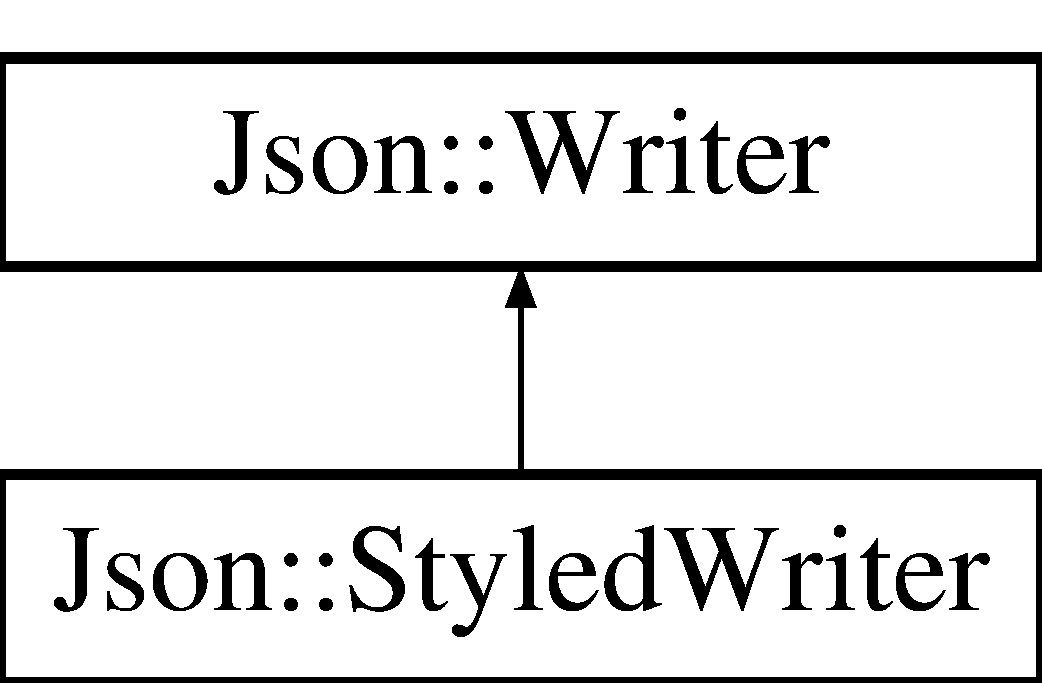
\includegraphics[height=2.000000cm]{classJson_1_1StyledWriter}
\end{center}
\end{figure}
\subsection*{Public Member Functions}
\begin{DoxyCompactItemize}
\item 
\hyperlink{classJson_1_1StyledWriter_a1f1b5f922a6a0ef0e56c6dd2f6170192}{Styled\+Writer} ()
\item 
\hyperlink{classJson_1_1StyledWriter_a6a18380a4c5dd5e37a892dc182aac88c}{$\sim$\+Styled\+Writer} () \hyperlink{json_8hpp_a824d6199c91488107e443226fa6022c5}{J\+S\+O\+N\+C\+P\+P\+\_\+\+O\+V\+E\+R\+R\+I\+DE}
\item 
\hyperlink{json_8hpp_a1e723f95759de062585bc4a8fd3fa4be}{J\+S\+O\+N\+C\+P\+P\+\_\+\+S\+T\+R\+I\+NG} \hyperlink{classJson_1_1StyledWriter_a5efab19b9746da9920c29cdae3a6b404}{write} (const \hyperlink{classJson_1_1Value}{Value} \&root) \hyperlink{json_8hpp_a824d6199c91488107e443226fa6022c5}{J\+S\+O\+N\+C\+P\+P\+\_\+\+O\+V\+E\+R\+R\+I\+DE}
\begin{DoxyCompactList}\small\item\em Serialize a \hyperlink{classJson_1_1Value}{Value} in \href{http://www.json.org}{\tt J\+S\+ON} format. \end{DoxyCompactList}\end{DoxyCompactItemize}
\subsection*{Private Types}
\begin{DoxyCompactItemize}
\item 
typedef std\+::vector$<$ \hyperlink{json_8hpp_a1e723f95759de062585bc4a8fd3fa4be}{J\+S\+O\+N\+C\+P\+P\+\_\+\+S\+T\+R\+I\+NG} $>$ \hyperlink{classJson_1_1StyledWriter_a798fcefa41730de612a5cf7e73003e8a}{Child\+Values}
\end{DoxyCompactItemize}
\subsection*{Private Member Functions}
\begin{DoxyCompactItemize}
\item 
void \hyperlink{classJson_1_1StyledWriter_ac40143cf43f7c4a94d3d0b41e5245069}{write\+Value} (const \hyperlink{classJson_1_1Value}{Value} \&value)
\item 
void \hyperlink{classJson_1_1StyledWriter_a0618c23d62965515def15ece1e677f5d}{write\+Array\+Value} (const \hyperlink{classJson_1_1Value}{Value} \&value)
\item 
bool \hyperlink{classJson_1_1StyledWriter_aa5dc671edf10b9976f1511da2271ab9d}{is\+Multine\+Array} (const \hyperlink{classJson_1_1Value}{Value} \&value)
\item 
void \hyperlink{classJson_1_1StyledWriter_a236a833b4bdaa09915c2cac715970f08}{push\+Value} (const \hyperlink{json_8hpp_a1e723f95759de062585bc4a8fd3fa4be}{J\+S\+O\+N\+C\+P\+P\+\_\+\+S\+T\+R\+I\+NG} \&value)
\item 
void \hyperlink{classJson_1_1StyledWriter_a885f4bfb5701896d60eee6716d2db7e4}{write\+Indent} ()
\item 
void \hyperlink{classJson_1_1StyledWriter_ac38e02972054125c38efbe327b52f6ac}{write\+With\+Indent} (const \hyperlink{json_8hpp_a1e723f95759de062585bc4a8fd3fa4be}{J\+S\+O\+N\+C\+P\+P\+\_\+\+S\+T\+R\+I\+NG} \&value)
\item 
void \hyperlink{classJson_1_1StyledWriter_a0b65be6186a7c6638270990265e42b97}{indent} ()
\item 
void \hyperlink{classJson_1_1StyledWriter_acee1c9285519b573cfcb00b7e7f5a809}{unindent} ()
\item 
void \hyperlink{classJson_1_1StyledWriter_ad3452c48fabf968bf3693549331ec06e}{write\+Comment\+Before\+Value} (const \hyperlink{classJson_1_1Value}{Value} \&root)
\item 
void \hyperlink{classJson_1_1StyledWriter_ab12b274c62822fc51ec4617c6be95139}{write\+Comment\+After\+Value\+On\+Same\+Line} (const \hyperlink{classJson_1_1Value}{Value} \&root)
\item 
bool \hyperlink{classJson_1_1StyledWriter_a37a806d010f708cb68556f2666f79bdf}{has\+Comment\+For\+Value} (const \hyperlink{classJson_1_1Value}{Value} \&value)
\end{DoxyCompactItemize}
\subsection*{Static Private Member Functions}
\begin{DoxyCompactItemize}
\item 
static \hyperlink{json_8hpp_a1e723f95759de062585bc4a8fd3fa4be}{J\+S\+O\+N\+C\+P\+P\+\_\+\+S\+T\+R\+I\+NG} \hyperlink{classJson_1_1StyledWriter_a692dda1b1621fb5620e0a7b1b10f3b1f}{normalize\+E\+OL} (const \hyperlink{json_8hpp_a1e723f95759de062585bc4a8fd3fa4be}{J\+S\+O\+N\+C\+P\+P\+\_\+\+S\+T\+R\+I\+NG} \&text)
\end{DoxyCompactItemize}
\subsection*{Private Attributes}
\begin{DoxyCompactItemize}
\item 
\hyperlink{classJson_1_1StyledWriter_a798fcefa41730de612a5cf7e73003e8a}{Child\+Values} \hyperlink{classJson_1_1StyledWriter_a1f905495f0705365af117ec541e29fdf}{child\+Values\+\_\+}
\item 
\hyperlink{json_8hpp_a1e723f95759de062585bc4a8fd3fa4be}{J\+S\+O\+N\+C\+P\+P\+\_\+\+S\+T\+R\+I\+NG} \hyperlink{classJson_1_1StyledWriter_ae967b0c77e4d7cb889ce7b6ee4ce28d7}{document\+\_\+}
\item 
\hyperlink{json_8hpp_a1e723f95759de062585bc4a8fd3fa4be}{J\+S\+O\+N\+C\+P\+P\+\_\+\+S\+T\+R\+I\+NG} \hyperlink{classJson_1_1StyledWriter_a7d91709c94c152bd44eaf80faac130ae}{indent\+String\+\_\+}
\item 
unsigned int \hyperlink{classJson_1_1StyledWriter_ae648d2e1fc0f7d45c748c96805106cb0}{right\+Margin\+\_\+}
\item 
unsigned int \hyperlink{classJson_1_1StyledWriter_a0b5ab768cc56433d463eb1f03da8614e}{indent\+Size\+\_\+}
\item 
bool \hyperlink{classJson_1_1StyledWriter_acaabfa48b50a8bb7fa9ce98e2ae971d9}{add\+Child\+Values\+\_\+}
\end{DoxyCompactItemize}


\subsection{Detailed Description}
Writes a \hyperlink{classJson_1_1Value}{Value} in \href{http://www.json.org}{\tt J\+S\+ON} format in a human friendly way. 

The rules for line break and indent are as follow\+:
\begin{DoxyItemize}
\item Object value\+:
\begin{DoxyItemize}
\item if empty then print \{\} without indent and line break
\item if not empty the print \textquotesingle{}\{\textquotesingle{}, line break \& indent, print one value per line and then unindent and line break and print \textquotesingle{}\}\textquotesingle{}.
\end{DoxyItemize}
\item Array value\+:
\begin{DoxyItemize}
\item if empty then print \mbox{[}\mbox{]} without indent and line break
\item if the array contains no object value, empty array or some other value types, and all the values fit on one lines, then print the array on a single line.
\item otherwise, it the values do not fit on one line, or the array contains object or non empty array, then print one value per line.
\end{DoxyItemize}
\end{DoxyItemize}

If the \hyperlink{classJson_1_1Value}{Value} have comments then they are outputed according to their \hyperlink{namespaceJson_a4fc417c23905b2ae9e2c47d197a45351}{Comment\+Placement}.

\begin{DoxySeeAlso}{See also}
\hyperlink{classJson_1_1Reader}{Reader}, \hyperlink{classJson_1_1Value}{Value}, \hyperlink{classJson_1_1Value_a29f3a30f7e5d3af6f38d57999bf5b480}{Value\+::set\+Comment()} 
\end{DoxySeeAlso}
\begin{DoxyRefDesc}{Deprecated}
\item[\hyperlink{deprecated__deprecated000009}{Deprecated}]Use \hyperlink{classJson_1_1StreamWriterBuilder}{Stream\+Writer\+Builder}. \end{DoxyRefDesc}


\subsection{Member Typedef Documentation}
\index{Json\+::\+Styled\+Writer@{Json\+::\+Styled\+Writer}!Child\+Values@{Child\+Values}}
\index{Child\+Values@{Child\+Values}!Json\+::\+Styled\+Writer@{Json\+::\+Styled\+Writer}}
\subsubsection[{\texorpdfstring{Child\+Values}{ChildValues}}]{\setlength{\rightskip}{0pt plus 5cm}typedef std\+::vector$<${\bf J\+S\+O\+N\+C\+P\+P\+\_\+\+S\+T\+R\+I\+NG}$>$ {\bf Json\+::\+Styled\+Writer\+::\+Child\+Values}\hspace{0.3cm}{\ttfamily [private]}}\hypertarget{classJson_1_1StyledWriter_a798fcefa41730de612a5cf7e73003e8a}{}\label{classJson_1_1StyledWriter_a798fcefa41730de612a5cf7e73003e8a}


\subsection{Constructor \& Destructor Documentation}
\index{Json\+::\+Styled\+Writer@{Json\+::\+Styled\+Writer}!Styled\+Writer@{Styled\+Writer}}
\index{Styled\+Writer@{Styled\+Writer}!Json\+::\+Styled\+Writer@{Json\+::\+Styled\+Writer}}
\subsubsection[{\texorpdfstring{Styled\+Writer()}{StyledWriter()}}]{\setlength{\rightskip}{0pt plus 5cm}Json\+::\+Styled\+Writer\+::\+Styled\+Writer (
\begin{DoxyParamCaption}
{}
\end{DoxyParamCaption}
)}\hypertarget{classJson_1_1StyledWriter_a1f1b5f922a6a0ef0e56c6dd2f6170192}{}\label{classJson_1_1StyledWriter_a1f1b5f922a6a0ef0e56c6dd2f6170192}
\index{Json\+::\+Styled\+Writer@{Json\+::\+Styled\+Writer}!````~Styled\+Writer@{$\sim$\+Styled\+Writer}}
\index{````~Styled\+Writer@{$\sim$\+Styled\+Writer}!Json\+::\+Styled\+Writer@{Json\+::\+Styled\+Writer}}
\subsubsection[{\texorpdfstring{$\sim$\+Styled\+Writer() J\+S\+O\+N\+C\+P\+P\+\_\+\+O\+V\+E\+R\+R\+I\+DE}{~StyledWriter() JSONCPP_OVERRIDE}}]{\setlength{\rightskip}{0pt plus 5cm}Json\+::\+Styled\+Writer\+::$\sim$\+Styled\+Writer (
\begin{DoxyParamCaption}
{}
\end{DoxyParamCaption}
)\hspace{0.3cm}{\ttfamily [inline]}}\hypertarget{classJson_1_1StyledWriter_a6a18380a4c5dd5e37a892dc182aac88c}{}\label{classJson_1_1StyledWriter_a6a18380a4c5dd5e37a892dc182aac88c}


\subsection{Member Function Documentation}
\index{Json\+::\+Styled\+Writer@{Json\+::\+Styled\+Writer}!has\+Comment\+For\+Value@{has\+Comment\+For\+Value}}
\index{has\+Comment\+For\+Value@{has\+Comment\+For\+Value}!Json\+::\+Styled\+Writer@{Json\+::\+Styled\+Writer}}
\subsubsection[{\texorpdfstring{has\+Comment\+For\+Value(const Value \&value)}{hasCommentForValue(const Value &value)}}]{\setlength{\rightskip}{0pt plus 5cm}bool Json\+::\+Styled\+Writer\+::has\+Comment\+For\+Value (
\begin{DoxyParamCaption}
\item[{const {\bf Value} \&}]{value}
\end{DoxyParamCaption}
)\hspace{0.3cm}{\ttfamily [private]}}\hypertarget{classJson_1_1StyledWriter_a37a806d010f708cb68556f2666f79bdf}{}\label{classJson_1_1StyledWriter_a37a806d010f708cb68556f2666f79bdf}
\index{Json\+::\+Styled\+Writer@{Json\+::\+Styled\+Writer}!indent@{indent}}
\index{indent@{indent}!Json\+::\+Styled\+Writer@{Json\+::\+Styled\+Writer}}
\subsubsection[{\texorpdfstring{indent()}{indent()}}]{\setlength{\rightskip}{0pt plus 5cm}void Json\+::\+Styled\+Writer\+::indent (
\begin{DoxyParamCaption}
{}
\end{DoxyParamCaption}
)\hspace{0.3cm}{\ttfamily [private]}}\hypertarget{classJson_1_1StyledWriter_a0b65be6186a7c6638270990265e42b97}{}\label{classJson_1_1StyledWriter_a0b65be6186a7c6638270990265e42b97}
\index{Json\+::\+Styled\+Writer@{Json\+::\+Styled\+Writer}!is\+Multine\+Array@{is\+Multine\+Array}}
\index{is\+Multine\+Array@{is\+Multine\+Array}!Json\+::\+Styled\+Writer@{Json\+::\+Styled\+Writer}}
\subsubsection[{\texorpdfstring{is\+Multine\+Array(const Value \&value)}{isMultineArray(const Value &value)}}]{\setlength{\rightskip}{0pt plus 5cm}bool Json\+::\+Styled\+Writer\+::is\+Multine\+Array (
\begin{DoxyParamCaption}
\item[{const {\bf Value} \&}]{value}
\end{DoxyParamCaption}
)\hspace{0.3cm}{\ttfamily [private]}}\hypertarget{classJson_1_1StyledWriter_aa5dc671edf10b9976f1511da2271ab9d}{}\label{classJson_1_1StyledWriter_aa5dc671edf10b9976f1511da2271ab9d}
\index{Json\+::\+Styled\+Writer@{Json\+::\+Styled\+Writer}!normalize\+E\+OL@{normalize\+E\+OL}}
\index{normalize\+E\+OL@{normalize\+E\+OL}!Json\+::\+Styled\+Writer@{Json\+::\+Styled\+Writer}}
\subsubsection[{\texorpdfstring{normalize\+E\+O\+L(const J\+S\+O\+N\+C\+P\+P\+\_\+\+S\+T\+R\+I\+N\+G \&text)}{normalizeEOL(const JSONCPP_STRING &text)}}]{\setlength{\rightskip}{0pt plus 5cm}static {\bf J\+S\+O\+N\+C\+P\+P\+\_\+\+S\+T\+R\+I\+NG} Json\+::\+Styled\+Writer\+::normalize\+E\+OL (
\begin{DoxyParamCaption}
\item[{const {\bf J\+S\+O\+N\+C\+P\+P\+\_\+\+S\+T\+R\+I\+NG} \&}]{text}
\end{DoxyParamCaption}
)\hspace{0.3cm}{\ttfamily [static]}, {\ttfamily [private]}}\hypertarget{classJson_1_1StyledWriter_a692dda1b1621fb5620e0a7b1b10f3b1f}{}\label{classJson_1_1StyledWriter_a692dda1b1621fb5620e0a7b1b10f3b1f}
\index{Json\+::\+Styled\+Writer@{Json\+::\+Styled\+Writer}!push\+Value@{push\+Value}}
\index{push\+Value@{push\+Value}!Json\+::\+Styled\+Writer@{Json\+::\+Styled\+Writer}}
\subsubsection[{\texorpdfstring{push\+Value(const J\+S\+O\+N\+C\+P\+P\+\_\+\+S\+T\+R\+I\+N\+G \&value)}{pushValue(const JSONCPP_STRING &value)}}]{\setlength{\rightskip}{0pt plus 5cm}void Json\+::\+Styled\+Writer\+::push\+Value (
\begin{DoxyParamCaption}
\item[{const {\bf J\+S\+O\+N\+C\+P\+P\+\_\+\+S\+T\+R\+I\+NG} \&}]{value}
\end{DoxyParamCaption}
)\hspace{0.3cm}{\ttfamily [private]}}\hypertarget{classJson_1_1StyledWriter_a236a833b4bdaa09915c2cac715970f08}{}\label{classJson_1_1StyledWriter_a236a833b4bdaa09915c2cac715970f08}
\index{Json\+::\+Styled\+Writer@{Json\+::\+Styled\+Writer}!unindent@{unindent}}
\index{unindent@{unindent}!Json\+::\+Styled\+Writer@{Json\+::\+Styled\+Writer}}
\subsubsection[{\texorpdfstring{unindent()}{unindent()}}]{\setlength{\rightskip}{0pt plus 5cm}void Json\+::\+Styled\+Writer\+::unindent (
\begin{DoxyParamCaption}
{}
\end{DoxyParamCaption}
)\hspace{0.3cm}{\ttfamily [private]}}\hypertarget{classJson_1_1StyledWriter_acee1c9285519b573cfcb00b7e7f5a809}{}\label{classJson_1_1StyledWriter_acee1c9285519b573cfcb00b7e7f5a809}
\index{Json\+::\+Styled\+Writer@{Json\+::\+Styled\+Writer}!write@{write}}
\index{write@{write}!Json\+::\+Styled\+Writer@{Json\+::\+Styled\+Writer}}
\subsubsection[{\texorpdfstring{write(const Value \&root) J\+S\+O\+N\+C\+P\+P\+\_\+\+O\+V\+E\+R\+R\+I\+DE}{write(const Value &root) JSONCPP_OVERRIDE}}]{\setlength{\rightskip}{0pt plus 5cm}{\bf J\+S\+O\+N\+C\+P\+P\+\_\+\+S\+T\+R\+I\+NG} Json\+::\+Styled\+Writer\+::write (
\begin{DoxyParamCaption}
\item[{const {\bf Value} \&}]{root}
\end{DoxyParamCaption}
)\hspace{0.3cm}{\ttfamily [virtual]}}\hypertarget{classJson_1_1StyledWriter_a5efab19b9746da9920c29cdae3a6b404}{}\label{classJson_1_1StyledWriter_a5efab19b9746da9920c29cdae3a6b404}


Serialize a \hyperlink{classJson_1_1Value}{Value} in \href{http://www.json.org}{\tt J\+S\+ON} format. 


\begin{DoxyParams}{Parameters}
{\em root} & \hyperlink{classJson_1_1Value}{Value} to serialize. \\
\hline
\end{DoxyParams}
\begin{DoxyReturn}{Returns}
String containing the J\+S\+ON document that represents the root value. 
\end{DoxyReturn}


Implements \hyperlink{classJson_1_1Writer_a61c55882b82c7651d0b9b683c6d3f371}{Json\+::\+Writer}.

\index{Json\+::\+Styled\+Writer@{Json\+::\+Styled\+Writer}!write\+Array\+Value@{write\+Array\+Value}}
\index{write\+Array\+Value@{write\+Array\+Value}!Json\+::\+Styled\+Writer@{Json\+::\+Styled\+Writer}}
\subsubsection[{\texorpdfstring{write\+Array\+Value(const Value \&value)}{writeArrayValue(const Value &value)}}]{\setlength{\rightskip}{0pt plus 5cm}void Json\+::\+Styled\+Writer\+::write\+Array\+Value (
\begin{DoxyParamCaption}
\item[{const {\bf Value} \&}]{value}
\end{DoxyParamCaption}
)\hspace{0.3cm}{\ttfamily [private]}}\hypertarget{classJson_1_1StyledWriter_a0618c23d62965515def15ece1e677f5d}{}\label{classJson_1_1StyledWriter_a0618c23d62965515def15ece1e677f5d}
\index{Json\+::\+Styled\+Writer@{Json\+::\+Styled\+Writer}!write\+Comment\+After\+Value\+On\+Same\+Line@{write\+Comment\+After\+Value\+On\+Same\+Line}}
\index{write\+Comment\+After\+Value\+On\+Same\+Line@{write\+Comment\+After\+Value\+On\+Same\+Line}!Json\+::\+Styled\+Writer@{Json\+::\+Styled\+Writer}}
\subsubsection[{\texorpdfstring{write\+Comment\+After\+Value\+On\+Same\+Line(const Value \&root)}{writeCommentAfterValueOnSameLine(const Value &root)}}]{\setlength{\rightskip}{0pt plus 5cm}void Json\+::\+Styled\+Writer\+::write\+Comment\+After\+Value\+On\+Same\+Line (
\begin{DoxyParamCaption}
\item[{const {\bf Value} \&}]{root}
\end{DoxyParamCaption}
)\hspace{0.3cm}{\ttfamily [private]}}\hypertarget{classJson_1_1StyledWriter_ab12b274c62822fc51ec4617c6be95139}{}\label{classJson_1_1StyledWriter_ab12b274c62822fc51ec4617c6be95139}
\index{Json\+::\+Styled\+Writer@{Json\+::\+Styled\+Writer}!write\+Comment\+Before\+Value@{write\+Comment\+Before\+Value}}
\index{write\+Comment\+Before\+Value@{write\+Comment\+Before\+Value}!Json\+::\+Styled\+Writer@{Json\+::\+Styled\+Writer}}
\subsubsection[{\texorpdfstring{write\+Comment\+Before\+Value(const Value \&root)}{writeCommentBeforeValue(const Value &root)}}]{\setlength{\rightskip}{0pt plus 5cm}void Json\+::\+Styled\+Writer\+::write\+Comment\+Before\+Value (
\begin{DoxyParamCaption}
\item[{const {\bf Value} \&}]{root}
\end{DoxyParamCaption}
)\hspace{0.3cm}{\ttfamily [private]}}\hypertarget{classJson_1_1StyledWriter_ad3452c48fabf968bf3693549331ec06e}{}\label{classJson_1_1StyledWriter_ad3452c48fabf968bf3693549331ec06e}
\index{Json\+::\+Styled\+Writer@{Json\+::\+Styled\+Writer}!write\+Indent@{write\+Indent}}
\index{write\+Indent@{write\+Indent}!Json\+::\+Styled\+Writer@{Json\+::\+Styled\+Writer}}
\subsubsection[{\texorpdfstring{write\+Indent()}{writeIndent()}}]{\setlength{\rightskip}{0pt plus 5cm}void Json\+::\+Styled\+Writer\+::write\+Indent (
\begin{DoxyParamCaption}
{}
\end{DoxyParamCaption}
)\hspace{0.3cm}{\ttfamily [private]}}\hypertarget{classJson_1_1StyledWriter_a885f4bfb5701896d60eee6716d2db7e4}{}\label{classJson_1_1StyledWriter_a885f4bfb5701896d60eee6716d2db7e4}
\index{Json\+::\+Styled\+Writer@{Json\+::\+Styled\+Writer}!write\+Value@{write\+Value}}
\index{write\+Value@{write\+Value}!Json\+::\+Styled\+Writer@{Json\+::\+Styled\+Writer}}
\subsubsection[{\texorpdfstring{write\+Value(const Value \&value)}{writeValue(const Value &value)}}]{\setlength{\rightskip}{0pt plus 5cm}void Json\+::\+Styled\+Writer\+::write\+Value (
\begin{DoxyParamCaption}
\item[{const {\bf Value} \&}]{value}
\end{DoxyParamCaption}
)\hspace{0.3cm}{\ttfamily [private]}}\hypertarget{classJson_1_1StyledWriter_ac40143cf43f7c4a94d3d0b41e5245069}{}\label{classJson_1_1StyledWriter_ac40143cf43f7c4a94d3d0b41e5245069}
\index{Json\+::\+Styled\+Writer@{Json\+::\+Styled\+Writer}!write\+With\+Indent@{write\+With\+Indent}}
\index{write\+With\+Indent@{write\+With\+Indent}!Json\+::\+Styled\+Writer@{Json\+::\+Styled\+Writer}}
\subsubsection[{\texorpdfstring{write\+With\+Indent(const J\+S\+O\+N\+C\+P\+P\+\_\+\+S\+T\+R\+I\+N\+G \&value)}{writeWithIndent(const JSONCPP_STRING &value)}}]{\setlength{\rightskip}{0pt plus 5cm}void Json\+::\+Styled\+Writer\+::write\+With\+Indent (
\begin{DoxyParamCaption}
\item[{const {\bf J\+S\+O\+N\+C\+P\+P\+\_\+\+S\+T\+R\+I\+NG} \&}]{value}
\end{DoxyParamCaption}
)\hspace{0.3cm}{\ttfamily [private]}}\hypertarget{classJson_1_1StyledWriter_ac38e02972054125c38efbe327b52f6ac}{}\label{classJson_1_1StyledWriter_ac38e02972054125c38efbe327b52f6ac}


\subsection{Member Data Documentation}
\index{Json\+::\+Styled\+Writer@{Json\+::\+Styled\+Writer}!add\+Child\+Values\+\_\+@{add\+Child\+Values\+\_\+}}
\index{add\+Child\+Values\+\_\+@{add\+Child\+Values\+\_\+}!Json\+::\+Styled\+Writer@{Json\+::\+Styled\+Writer}}
\subsubsection[{\texorpdfstring{add\+Child\+Values\+\_\+}{addChildValues_}}]{\setlength{\rightskip}{0pt plus 5cm}bool Json\+::\+Styled\+Writer\+::add\+Child\+Values\+\_\+\hspace{0.3cm}{\ttfamily [private]}}\hypertarget{classJson_1_1StyledWriter_acaabfa48b50a8bb7fa9ce98e2ae971d9}{}\label{classJson_1_1StyledWriter_acaabfa48b50a8bb7fa9ce98e2ae971d9}
\index{Json\+::\+Styled\+Writer@{Json\+::\+Styled\+Writer}!child\+Values\+\_\+@{child\+Values\+\_\+}}
\index{child\+Values\+\_\+@{child\+Values\+\_\+}!Json\+::\+Styled\+Writer@{Json\+::\+Styled\+Writer}}
\subsubsection[{\texorpdfstring{child\+Values\+\_\+}{childValues_}}]{\setlength{\rightskip}{0pt plus 5cm}{\bf Child\+Values} Json\+::\+Styled\+Writer\+::child\+Values\+\_\+\hspace{0.3cm}{\ttfamily [private]}}\hypertarget{classJson_1_1StyledWriter_a1f905495f0705365af117ec541e29fdf}{}\label{classJson_1_1StyledWriter_a1f905495f0705365af117ec541e29fdf}
\index{Json\+::\+Styled\+Writer@{Json\+::\+Styled\+Writer}!document\+\_\+@{document\+\_\+}}
\index{document\+\_\+@{document\+\_\+}!Json\+::\+Styled\+Writer@{Json\+::\+Styled\+Writer}}
\subsubsection[{\texorpdfstring{document\+\_\+}{document_}}]{\setlength{\rightskip}{0pt plus 5cm}{\bf J\+S\+O\+N\+C\+P\+P\+\_\+\+S\+T\+R\+I\+NG} Json\+::\+Styled\+Writer\+::document\+\_\+\hspace{0.3cm}{\ttfamily [private]}}\hypertarget{classJson_1_1StyledWriter_ae967b0c77e4d7cb889ce7b6ee4ce28d7}{}\label{classJson_1_1StyledWriter_ae967b0c77e4d7cb889ce7b6ee4ce28d7}
\index{Json\+::\+Styled\+Writer@{Json\+::\+Styled\+Writer}!indent\+Size\+\_\+@{indent\+Size\+\_\+}}
\index{indent\+Size\+\_\+@{indent\+Size\+\_\+}!Json\+::\+Styled\+Writer@{Json\+::\+Styled\+Writer}}
\subsubsection[{\texorpdfstring{indent\+Size\+\_\+}{indentSize_}}]{\setlength{\rightskip}{0pt plus 5cm}unsigned int Json\+::\+Styled\+Writer\+::indent\+Size\+\_\+\hspace{0.3cm}{\ttfamily [private]}}\hypertarget{classJson_1_1StyledWriter_a0b5ab768cc56433d463eb1f03da8614e}{}\label{classJson_1_1StyledWriter_a0b5ab768cc56433d463eb1f03da8614e}
\index{Json\+::\+Styled\+Writer@{Json\+::\+Styled\+Writer}!indent\+String\+\_\+@{indent\+String\+\_\+}}
\index{indent\+String\+\_\+@{indent\+String\+\_\+}!Json\+::\+Styled\+Writer@{Json\+::\+Styled\+Writer}}
\subsubsection[{\texorpdfstring{indent\+String\+\_\+}{indentString_}}]{\setlength{\rightskip}{0pt plus 5cm}{\bf J\+S\+O\+N\+C\+P\+P\+\_\+\+S\+T\+R\+I\+NG} Json\+::\+Styled\+Writer\+::indent\+String\+\_\+\hspace{0.3cm}{\ttfamily [private]}}\hypertarget{classJson_1_1StyledWriter_a7d91709c94c152bd44eaf80faac130ae}{}\label{classJson_1_1StyledWriter_a7d91709c94c152bd44eaf80faac130ae}
\index{Json\+::\+Styled\+Writer@{Json\+::\+Styled\+Writer}!right\+Margin\+\_\+@{right\+Margin\+\_\+}}
\index{right\+Margin\+\_\+@{right\+Margin\+\_\+}!Json\+::\+Styled\+Writer@{Json\+::\+Styled\+Writer}}
\subsubsection[{\texorpdfstring{right\+Margin\+\_\+}{rightMargin_}}]{\setlength{\rightskip}{0pt plus 5cm}unsigned int Json\+::\+Styled\+Writer\+::right\+Margin\+\_\+\hspace{0.3cm}{\ttfamily [private]}}\hypertarget{classJson_1_1StyledWriter_ae648d2e1fc0f7d45c748c96805106cb0}{}\label{classJson_1_1StyledWriter_ae648d2e1fc0f7d45c748c96805106cb0}


The documentation for this class was generated from the following files\+:\begin{DoxyCompactItemize}
\item 
/home/pranav/\+Repositories/zcm/include/\hyperlink{json_8hpp}{json.\+hpp}\item 
/home/pranav/\+Repositories/zcm/src/\hyperlink{json_8cpp}{json.\+cpp}\end{DoxyCompactItemize}

\hypertarget{classzcm_1_1Subscriber}{\section{zcm\-:\-:Subscriber Class Reference}
\label{classzcm_1_1Subscriber}\index{zcm\-::\-Subscriber@{zcm\-::\-Subscriber}}
}


\hyperlink{classzcm_1_1Subscriber}{Subscriber} class.  




{\ttfamily \#include $<$subscriber.\-hpp$>$}

\subsection*{Public Member Functions}
\begin{DoxyCompactItemize}
\item 
\hyperlink{classzcm_1_1Subscriber_a8477e4359c83f009ad34bbbd5e0c7b68}{Subscriber} (std\-::string \hyperlink{classzcm_1_1Subscriber_a2ec3b22204d0f3f72e996b19b086910b}{name}, unsigned int \hyperlink{classzcm_1_1Subscriber_a208baedba808c9229887ab8af00725fd}{priority}, zmq\-::context\-\_\-t $\ast$actor\-\_\-context, std\-::string \hyperlink{classzcm_1_1Subscriber_a28ab0921d97bc4d05ac6bb64c977cc35}{filter}, std\-::function$<$ void()$>$ \hyperlink{classzcm_1_1Subscriber_ab8e52c24d7dc57b33d2c1536de4197b2}{operation\-\_\-function}, \hyperlink{classzcm_1_1Operation__Queue}{Operation\-\_\-\-Queue} $\ast$\hyperlink{classzcm_1_1Subscriber_a1cd579aa570832f9656b9fa24747dde3}{operation\-\_\-queue\-\_\-ptr})
\begin{DoxyCompactList}\small\item\em Construct a subscriber object. \end{DoxyCompactList}\item 
\hyperlink{classzcm_1_1Subscriber_a248ea0aab7fc2d283f5373e33abd7287}{Subscriber} (std\-::string \hyperlink{classzcm_1_1Subscriber_a2ec3b22204d0f3f72e996b19b086910b}{name}, unsigned int \hyperlink{classzcm_1_1Subscriber_a208baedba808c9229887ab8af00725fd}{priority}, zmq\-::context\-\_\-t $\ast$actor\-\_\-context, std\-::string \hyperlink{classzcm_1_1Subscriber_a28ab0921d97bc4d05ac6bb64c977cc35}{filter}, std\-::vector$<$ std\-::string $>$ \hyperlink{classzcm_1_1Subscriber_a81590d7017038d6f50073baaa485a1b7}{endpoints}, std\-::function$<$ void()$>$ \hyperlink{classzcm_1_1Subscriber_ab8e52c24d7dc57b33d2c1536de4197b2}{operation\-\_\-function}, \hyperlink{classzcm_1_1Operation__Queue}{Operation\-\_\-\-Queue} $\ast$\hyperlink{classzcm_1_1Subscriber_a1cd579aa570832f9656b9fa24747dde3}{operation\-\_\-queue\-\_\-ptr})
\begin{DoxyCompactList}\small\item\em Construct a subscriber object with known endpoints. \end{DoxyCompactList}\item 
\hyperlink{classzcm_1_1Subscriber_a6f647c7d9f952e07b22b3aa4b63778e7}{$\sim$\-Subscriber} ()
\begin{DoxyCompactList}\small\item\em Close the subscriber socket and destroy the Z\-M\-Q context. \end{DoxyCompactList}\item 
void \hyperlink{classzcm_1_1Subscriber_a542674cff70f8d22b490a6b4a87476fe}{connect} (std\-::vector$<$ std\-::string $>$ new\-\_\-endpoints)
\begin{DoxyCompactList}\small\item\em Connect to a new set of endpoints param\mbox{[}in\mbox{]} new\-\_\-endpoints A new vector of endpoints to connect to. \end{DoxyCompactList}\item 
std\-::string \hyperlink{classzcm_1_1Subscriber_a013f450dff91644668a84cdb65d51b53}{get\-\_\-name} ()
\begin{DoxyCompactList}\small\item\em Get the name of the subscriber. \end{DoxyCompactList}\item 
unsigned int \hyperlink{classzcm_1_1Subscriber_a67427b093be45c979b4f091e6a9831ab}{get\-\_\-priority} ()
\begin{DoxyCompactList}\small\item\em Get the priority of the subscriber. \end{DoxyCompactList}\item 
void \hyperlink{classzcm_1_1Subscriber_acbfe7d4ab1b4a6fad5d9a7cbd3b8ee09}{add\-\_\-connection} (std\-::string new\-\_\-connection)
\begin{DoxyCompactList}\small\item\em Add a new connection to the subscriber. \end{DoxyCompactList}\item 
void \hyperlink{classzcm_1_1Subscriber_a3e270344beb730e009d48b04792e5526}{recv} ()
\begin{DoxyCompactList}\small\item\em Thread function of the subscriber Behavior\-: (1) Wait for a new message on the subscriber Z\-M\-Q socket (2) Create a Susbcriber Operation (3) Enqueue onto operation\-\_\-queue (4) Goto step (1) \end{DoxyCompactList}\item 
void \hyperlink{classzcm_1_1Subscriber_a43497c10d058c40395b5541a20649816}{rebind\-\_\-operation\-\_\-function} (std\-::function$<$ void()$>$ new\-\_\-operation\-\_\-function)
\begin{DoxyCompactList}\small\item\em Rebind the subscriber operation function. \end{DoxyCompactList}\item 
std\-::thread \hyperlink{classzcm_1_1Subscriber_a05334a6b27ce47e46ad525c2fc015347}{spawn} ()
\begin{DoxyCompactList}\small\item\em Spawn a new thread for the subscriber. \end{DoxyCompactList}\item 
void \hyperlink{classzcm_1_1Subscriber_af255252bdc1808c7436208b919612a48}{start} ()
\begin{DoxyCompactList}\small\item\em Start the subscriber thread. \end{DoxyCompactList}\item 
bool \hyperlink{classzcm_1_1Subscriber_adabba1785e367df820f011fbdb2a52c2}{is\-\_\-buffer\-\_\-empty} ()
\begin{DoxyCompactList}\small\item\em Is the message buffer empty? \end{DoxyCompactList}\item 
std\-::string \hyperlink{classzcm_1_1Subscriber_a153a90da1c97e12da900d02b3726a207}{message} ()
\begin{DoxyCompactList}\small\item\em Is the message buffer empty? \end{DoxyCompactList}\end{DoxyCompactItemize}
\subsection*{Private Attributes}
\begin{DoxyCompactItemize}
\item 
std\-::string \hyperlink{classzcm_1_1Subscriber_a2ec3b22204d0f3f72e996b19b086910b}{name}
\begin{DoxyCompactList}\small\item\em Name of the subscriber. \end{DoxyCompactList}\item 
unsigned int \hyperlink{classzcm_1_1Subscriber_a208baedba808c9229887ab8af00725fd}{priority}
\begin{DoxyCompactList}\small\item\em Priority of the subscriber. \end{DoxyCompactList}\item 
zmq\-::context\-\_\-t $\ast$ \hyperlink{classzcm_1_1Subscriber_a271ab3c945d1d3a84551bdca5e50f83f}{context}
\begin{DoxyCompactList}\small\item\em Pointer to the subscriber Z\-M\-Q context. \end{DoxyCompactList}\item 
std\-::string \hyperlink{classzcm_1_1Subscriber_a28ab0921d97bc4d05ac6bb64c977cc35}{filter}
\begin{DoxyCompactList}\small\item\em Reception filter enforced on all received messages. \end{DoxyCompactList}\item 
std\-::vector$<$ std\-::string $>$ \hyperlink{classzcm_1_1Subscriber_a81590d7017038d6f50073baaa485a1b7}{endpoints}
\begin{DoxyCompactList}\small\item\em Vector of connection endpoints. \end{DoxyCompactList}\item 
std\-::function$<$ void()$>$ \hyperlink{classzcm_1_1Subscriber_ab8e52c24d7dc57b33d2c1536de4197b2}{operation\-\_\-function}
\begin{DoxyCompactList}\small\item\em Operation function bound to the subscriber. \end{DoxyCompactList}\item 
\hyperlink{classzcm_1_1Operation__Queue}{Operation\-\_\-\-Queue} $\ast$ \hyperlink{classzcm_1_1Subscriber_a1cd579aa570832f9656b9fa24747dde3}{operation\-\_\-queue\-\_\-ptr}
\begin{DoxyCompactList}\small\item\em Pointer to the operation queue. \end{DoxyCompactList}\item 
zmq\-::socket\-\_\-t $\ast$ \hyperlink{classzcm_1_1Subscriber_ab6b9ee85d97a209b7c370b90882ed028}{subscriber\-\_\-socket}
\begin{DoxyCompactList}\small\item\em Pointer to the subscriber Z\-M\-Q socket. \end{DoxyCompactList}\item 
std\-::mutex \hyperlink{classzcm_1_1Subscriber_abd7e5c8f6ab6ce6e8854d8d407476c25}{func\-\_\-mutex}
\begin{DoxyCompactList}\small\item\em Mutex used to change operation\-\_\-function at runtime. \end{DoxyCompactList}\item 
std\-::queue$<$ std\-::string $>$ \hyperlink{classzcm_1_1Subscriber_a0f4c8918c98ebfdebfd46a21d6794a0b}{buffer}
\begin{DoxyCompactList}\small\item\em Buffer of messages received by the subscriber. \end{DoxyCompactList}\end{DoxyCompactItemize}


\subsection{Detailed Description}
\hyperlink{classzcm_1_1Subscriber}{Subscriber} class. 

\subsection{Constructor \& Destructor Documentation}
\hypertarget{classzcm_1_1Subscriber_a8477e4359c83f009ad34bbbd5e0c7b68}{\index{zcm\-::\-Subscriber@{zcm\-::\-Subscriber}!Subscriber@{Subscriber}}
\index{Subscriber@{Subscriber}!zcm::Subscriber@{zcm\-::\-Subscriber}}
\subsubsection[{Subscriber}]{\setlength{\rightskip}{0pt plus 5cm}zcm\-::\-Subscriber\-::\-Subscriber (
\begin{DoxyParamCaption}
\item[{std\-::string}]{name, }
\item[{unsigned int}]{priority, }
\item[{zmq\-::context\-\_\-t $\ast$}]{actor\-\_\-context, }
\item[{std\-::string}]{filter, }
\item[{std\-::function$<$ void()$>$}]{operation\-\_\-function, }
\item[{{\bf Operation\-\_\-\-Queue} $\ast$}]{operation\-\_\-queue\-\_\-ptr}
\end{DoxyParamCaption}
)\hspace{0.3cm}{\ttfamily [inline]}}}\label{classzcm_1_1Subscriber_a8477e4359c83f009ad34bbbd5e0c7b68}


Construct a subscriber object. 


\begin{DoxyParams}[1]{Parameters}
\mbox{\tt in}  & {\em name} & \hyperlink{classzcm_1_1Subscriber}{Subscriber} name \\
\hline
\mbox{\tt in}  & {\em priority} & Priority of the subscriber \\
\hline
\mbox{\tt in}  & {\em Z\-M\-Q} & Context of the \hyperlink{classzcm_1_1Actor}{Actor} Process \\
\hline
\mbox{\tt in}  & {\em filter} & Z\-M\-Q filter for the subscriber \\
\hline
\mbox{\tt in}  & {\em operation\-\_\-function} & Operation function of the subscriber \\
\hline
\mbox{\tt in}  & {\em operation\-\_\-queue\-\_\-ptr} & Pointer to the operation queue \\
\hline
\end{DoxyParams}
\hypertarget{classzcm_1_1Subscriber_a248ea0aab7fc2d283f5373e33abd7287}{\index{zcm\-::\-Subscriber@{zcm\-::\-Subscriber}!Subscriber@{Subscriber}}
\index{Subscriber@{Subscriber}!zcm::Subscriber@{zcm\-::\-Subscriber}}
\subsubsection[{Subscriber}]{\setlength{\rightskip}{0pt plus 5cm}zcm\-::\-Subscriber\-::\-Subscriber (
\begin{DoxyParamCaption}
\item[{std\-::string}]{name, }
\item[{unsigned int}]{priority, }
\item[{zmq\-::context\-\_\-t $\ast$}]{actor\-\_\-context, }
\item[{std\-::string}]{filter, }
\item[{std\-::vector$<$ std\-::string $>$}]{endpoints, }
\item[{std\-::function$<$ void()$>$}]{operation\-\_\-function, }
\item[{{\bf Operation\-\_\-\-Queue} $\ast$}]{operation\-\_\-queue\-\_\-ptr}
\end{DoxyParamCaption}
)}}\label{classzcm_1_1Subscriber_a248ea0aab7fc2d283f5373e33abd7287}


Construct a subscriber object with known endpoints. 


\begin{DoxyParams}[1]{Parameters}
\mbox{\tt in}  & {\em name} & \hyperlink{classzcm_1_1Subscriber}{Subscriber} name \\
\hline
\mbox{\tt in}  & {\em priority} & Priority of the subscriber \\
\hline
\mbox{\tt in}  & {\em Z\-M\-Q} & Context of the \hyperlink{classzcm_1_1Actor}{Actor} Process \\
\hline
\mbox{\tt in}  & {\em filter} & Z\-M\-Q filter for the subscriber \\
\hline
\mbox{\tt in}  & {\em endpoints} & A vector of endpoints to connect to \\
\hline
\mbox{\tt in}  & {\em operation\-\_\-function} & Operation function of the subscriber \\
\hline
\mbox{\tt in}  & {\em operation\-\_\-queue\-\_\-ptr} & Pointer to the operation queue \\
\hline
\end{DoxyParams}
\hypertarget{classzcm_1_1Subscriber_a6f647c7d9f952e07b22b3aa4b63778e7}{\index{zcm\-::\-Subscriber@{zcm\-::\-Subscriber}!$\sim$\-Subscriber@{$\sim$\-Subscriber}}
\index{$\sim$\-Subscriber@{$\sim$\-Subscriber}!zcm::Subscriber@{zcm\-::\-Subscriber}}
\subsubsection[{$\sim$\-Subscriber}]{\setlength{\rightskip}{0pt plus 5cm}zcm\-::\-Subscriber\-::$\sim$\-Subscriber (
\begin{DoxyParamCaption}
{}
\end{DoxyParamCaption}
)}}\label{classzcm_1_1Subscriber_a6f647c7d9f952e07b22b3aa4b63778e7}


Close the subscriber socket and destroy the Z\-M\-Q context. 



\subsection{Member Function Documentation}
\hypertarget{classzcm_1_1Subscriber_acbfe7d4ab1b4a6fad5d9a7cbd3b8ee09}{\index{zcm\-::\-Subscriber@{zcm\-::\-Subscriber}!add\-\_\-connection@{add\-\_\-connection}}
\index{add\-\_\-connection@{add\-\_\-connection}!zcm::Subscriber@{zcm\-::\-Subscriber}}
\subsubsection[{add\-\_\-connection}]{\setlength{\rightskip}{0pt plus 5cm}void zcm\-::\-Subscriber\-::add\-\_\-connection (
\begin{DoxyParamCaption}
\item[{std\-::string}]{new\-\_\-connection}
\end{DoxyParamCaption}
)}}\label{classzcm_1_1Subscriber_acbfe7d4ab1b4a6fad5d9a7cbd3b8ee09}


Add a new connection to the subscriber. 


\begin{DoxyParams}[1]{Parameters}
\mbox{\tt in}  & {\em new\-\_\-connection} & New connection address to connect to \\
\hline
\end{DoxyParams}
\hypertarget{classzcm_1_1Subscriber_a542674cff70f8d22b490a6b4a87476fe}{\index{zcm\-::\-Subscriber@{zcm\-::\-Subscriber}!connect@{connect}}
\index{connect@{connect}!zcm::Subscriber@{zcm\-::\-Subscriber}}
\subsubsection[{connect}]{\setlength{\rightskip}{0pt plus 5cm}void zcm\-::\-Subscriber\-::connect (
\begin{DoxyParamCaption}
\item[{std\-::vector$<$ std\-::string $>$}]{new\-\_\-endpoints}
\end{DoxyParamCaption}
)}}\label{classzcm_1_1Subscriber_a542674cff70f8d22b490a6b4a87476fe}


Connect to a new set of endpoints param\mbox{[}in\mbox{]} new\-\_\-endpoints A new vector of endpoints to connect to. 

\hypertarget{classzcm_1_1Subscriber_a013f450dff91644668a84cdb65d51b53}{\index{zcm\-::\-Subscriber@{zcm\-::\-Subscriber}!get\-\_\-name@{get\-\_\-name}}
\index{get\-\_\-name@{get\-\_\-name}!zcm::Subscriber@{zcm\-::\-Subscriber}}
\subsubsection[{get\-\_\-name}]{\setlength{\rightskip}{0pt plus 5cm}std\-::string zcm\-::\-Subscriber\-::get\-\_\-name (
\begin{DoxyParamCaption}
{}
\end{DoxyParamCaption}
)}}\label{classzcm_1_1Subscriber_a013f450dff91644668a84cdb65d51b53}


Get the name of the subscriber. 

\hypertarget{classzcm_1_1Subscriber_a67427b093be45c979b4f091e6a9831ab}{\index{zcm\-::\-Subscriber@{zcm\-::\-Subscriber}!get\-\_\-priority@{get\-\_\-priority}}
\index{get\-\_\-priority@{get\-\_\-priority}!zcm::Subscriber@{zcm\-::\-Subscriber}}
\subsubsection[{get\-\_\-priority}]{\setlength{\rightskip}{0pt plus 5cm}unsigned int zcm\-::\-Subscriber\-::get\-\_\-priority (
\begin{DoxyParamCaption}
{}
\end{DoxyParamCaption}
)}}\label{classzcm_1_1Subscriber_a67427b093be45c979b4f091e6a9831ab}


Get the priority of the subscriber. 

\hypertarget{classzcm_1_1Subscriber_adabba1785e367df820f011fbdb2a52c2}{\index{zcm\-::\-Subscriber@{zcm\-::\-Subscriber}!is\-\_\-buffer\-\_\-empty@{is\-\_\-buffer\-\_\-empty}}
\index{is\-\_\-buffer\-\_\-empty@{is\-\_\-buffer\-\_\-empty}!zcm::Subscriber@{zcm\-::\-Subscriber}}
\subsubsection[{is\-\_\-buffer\-\_\-empty}]{\setlength{\rightskip}{0pt plus 5cm}bool zcm\-::\-Subscriber\-::is\-\_\-buffer\-\_\-empty (
\begin{DoxyParamCaption}
{}
\end{DoxyParamCaption}
)}}\label{classzcm_1_1Subscriber_adabba1785e367df820f011fbdb2a52c2}


Is the message buffer empty? 

\hypertarget{classzcm_1_1Subscriber_a153a90da1c97e12da900d02b3726a207}{\index{zcm\-::\-Subscriber@{zcm\-::\-Subscriber}!message@{message}}
\index{message@{message}!zcm::Subscriber@{zcm\-::\-Subscriber}}
\subsubsection[{message}]{\setlength{\rightskip}{0pt plus 5cm}std\-::string zcm\-::\-Subscriber\-::message (
\begin{DoxyParamCaption}
{}
\end{DoxyParamCaption}
)}}\label{classzcm_1_1Subscriber_a153a90da1c97e12da900d02b3726a207}


Is the message buffer empty? 

\hypertarget{classzcm_1_1Subscriber_a43497c10d058c40395b5541a20649816}{\index{zcm\-::\-Subscriber@{zcm\-::\-Subscriber}!rebind\-\_\-operation\-\_\-function@{rebind\-\_\-operation\-\_\-function}}
\index{rebind\-\_\-operation\-\_\-function@{rebind\-\_\-operation\-\_\-function}!zcm::Subscriber@{zcm\-::\-Subscriber}}
\subsubsection[{rebind\-\_\-operation\-\_\-function}]{\setlength{\rightskip}{0pt plus 5cm}void zcm\-::\-Subscriber\-::rebind\-\_\-operation\-\_\-function (
\begin{DoxyParamCaption}
\item[{std\-::function$<$ void()$>$}]{new\-\_\-operation\-\_\-function}
\end{DoxyParamCaption}
)}}\label{classzcm_1_1Subscriber_a43497c10d058c40395b5541a20649816}


Rebind the subscriber operation function. 


\begin{DoxyParams}[1]{Parameters}
\mbox{\tt in}  & {\em new\-\_\-operation\-\_\-function} & New subscriber function to be handled upon \hyperlink{classzcm_1_1Subscriber_a3e270344beb730e009d48b04792e5526}{recv()} \\
\hline
\end{DoxyParams}
\hypertarget{classzcm_1_1Subscriber_a3e270344beb730e009d48b04792e5526}{\index{zcm\-::\-Subscriber@{zcm\-::\-Subscriber}!recv@{recv}}
\index{recv@{recv}!zcm::Subscriber@{zcm\-::\-Subscriber}}
\subsubsection[{recv}]{\setlength{\rightskip}{0pt plus 5cm}void zcm\-::\-Subscriber\-::recv (
\begin{DoxyParamCaption}
{}
\end{DoxyParamCaption}
)}}\label{classzcm_1_1Subscriber_a3e270344beb730e009d48b04792e5526}


Thread function of the subscriber Behavior\-: (1) Wait for a new message on the subscriber Z\-M\-Q socket (2) Create a Susbcriber Operation (3) Enqueue onto operation\-\_\-queue (4) Goto step (1) 

\hypertarget{classzcm_1_1Subscriber_a05334a6b27ce47e46ad525c2fc015347}{\index{zcm\-::\-Subscriber@{zcm\-::\-Subscriber}!spawn@{spawn}}
\index{spawn@{spawn}!zcm::Subscriber@{zcm\-::\-Subscriber}}
\subsubsection[{spawn}]{\setlength{\rightskip}{0pt plus 5cm}std\-::thread zcm\-::\-Subscriber\-::spawn (
\begin{DoxyParamCaption}
{}
\end{DoxyParamCaption}
)}}\label{classzcm_1_1Subscriber_a05334a6b27ce47e46ad525c2fc015347}


Spawn a new thread for the subscriber. 

\begin{DoxyReturn}{Returns}
\hyperlink{classzcm_1_1Subscriber}{Subscriber} thread 
\end{DoxyReturn}
\hypertarget{classzcm_1_1Subscriber_af255252bdc1808c7436208b919612a48}{\index{zcm\-::\-Subscriber@{zcm\-::\-Subscriber}!start@{start}}
\index{start@{start}!zcm::Subscriber@{zcm\-::\-Subscriber}}
\subsubsection[{start}]{\setlength{\rightskip}{0pt plus 5cm}void zcm\-::\-Subscriber\-::start (
\begin{DoxyParamCaption}
{}
\end{DoxyParamCaption}
)}}\label{classzcm_1_1Subscriber_af255252bdc1808c7436208b919612a48}


Start the subscriber thread. 



\subsection{Member Data Documentation}
\hypertarget{classzcm_1_1Subscriber_a0f4c8918c98ebfdebfd46a21d6794a0b}{\index{zcm\-::\-Subscriber@{zcm\-::\-Subscriber}!buffer@{buffer}}
\index{buffer@{buffer}!zcm::Subscriber@{zcm\-::\-Subscriber}}
\subsubsection[{buffer}]{\setlength{\rightskip}{0pt plus 5cm}std\-::queue$<$std\-::string$>$ zcm\-::\-Subscriber\-::buffer\hspace{0.3cm}{\ttfamily [private]}}}\label{classzcm_1_1Subscriber_a0f4c8918c98ebfdebfd46a21d6794a0b}


Buffer of messages received by the subscriber. 

\hypertarget{classzcm_1_1Subscriber_a271ab3c945d1d3a84551bdca5e50f83f}{\index{zcm\-::\-Subscriber@{zcm\-::\-Subscriber}!context@{context}}
\index{context@{context}!zcm::Subscriber@{zcm\-::\-Subscriber}}
\subsubsection[{context}]{\setlength{\rightskip}{0pt plus 5cm}zmq\-::context\-\_\-t$\ast$ zcm\-::\-Subscriber\-::context\hspace{0.3cm}{\ttfamily [private]}}}\label{classzcm_1_1Subscriber_a271ab3c945d1d3a84551bdca5e50f83f}


Pointer to the subscriber Z\-M\-Q context. 

\hypertarget{classzcm_1_1Subscriber_a81590d7017038d6f50073baaa485a1b7}{\index{zcm\-::\-Subscriber@{zcm\-::\-Subscriber}!endpoints@{endpoints}}
\index{endpoints@{endpoints}!zcm::Subscriber@{zcm\-::\-Subscriber}}
\subsubsection[{endpoints}]{\setlength{\rightskip}{0pt plus 5cm}std\-::vector$<$std\-::string$>$ zcm\-::\-Subscriber\-::endpoints\hspace{0.3cm}{\ttfamily [private]}}}\label{classzcm_1_1Subscriber_a81590d7017038d6f50073baaa485a1b7}


Vector of connection endpoints. 

\hypertarget{classzcm_1_1Subscriber_a28ab0921d97bc4d05ac6bb64c977cc35}{\index{zcm\-::\-Subscriber@{zcm\-::\-Subscriber}!filter@{filter}}
\index{filter@{filter}!zcm::Subscriber@{zcm\-::\-Subscriber}}
\subsubsection[{filter}]{\setlength{\rightskip}{0pt plus 5cm}std\-::string zcm\-::\-Subscriber\-::filter\hspace{0.3cm}{\ttfamily [private]}}}\label{classzcm_1_1Subscriber_a28ab0921d97bc4d05ac6bb64c977cc35}


Reception filter enforced on all received messages. 

\hypertarget{classzcm_1_1Subscriber_abd7e5c8f6ab6ce6e8854d8d407476c25}{\index{zcm\-::\-Subscriber@{zcm\-::\-Subscriber}!func\-\_\-mutex@{func\-\_\-mutex}}
\index{func\-\_\-mutex@{func\-\_\-mutex}!zcm::Subscriber@{zcm\-::\-Subscriber}}
\subsubsection[{func\-\_\-mutex}]{\setlength{\rightskip}{0pt plus 5cm}std\-::mutex zcm\-::\-Subscriber\-::func\-\_\-mutex\hspace{0.3cm}{\ttfamily [private]}}}\label{classzcm_1_1Subscriber_abd7e5c8f6ab6ce6e8854d8d407476c25}


Mutex used to change operation\-\_\-function at runtime. 

\hypertarget{classzcm_1_1Subscriber_a2ec3b22204d0f3f72e996b19b086910b}{\index{zcm\-::\-Subscriber@{zcm\-::\-Subscriber}!name@{name}}
\index{name@{name}!zcm::Subscriber@{zcm\-::\-Subscriber}}
\subsubsection[{name}]{\setlength{\rightskip}{0pt plus 5cm}std\-::string zcm\-::\-Subscriber\-::name\hspace{0.3cm}{\ttfamily [private]}}}\label{classzcm_1_1Subscriber_a2ec3b22204d0f3f72e996b19b086910b}


Name of the subscriber. 

\hypertarget{classzcm_1_1Subscriber_ab8e52c24d7dc57b33d2c1536de4197b2}{\index{zcm\-::\-Subscriber@{zcm\-::\-Subscriber}!operation\-\_\-function@{operation\-\_\-function}}
\index{operation\-\_\-function@{operation\-\_\-function}!zcm::Subscriber@{zcm\-::\-Subscriber}}
\subsubsection[{operation\-\_\-function}]{\setlength{\rightskip}{0pt plus 5cm}std\-::function$<$void()$>$ zcm\-::\-Subscriber\-::operation\-\_\-function\hspace{0.3cm}{\ttfamily [private]}}}\label{classzcm_1_1Subscriber_ab8e52c24d7dc57b33d2c1536de4197b2}


Operation function bound to the subscriber. 

\hypertarget{classzcm_1_1Subscriber_a1cd579aa570832f9656b9fa24747dde3}{\index{zcm\-::\-Subscriber@{zcm\-::\-Subscriber}!operation\-\_\-queue\-\_\-ptr@{operation\-\_\-queue\-\_\-ptr}}
\index{operation\-\_\-queue\-\_\-ptr@{operation\-\_\-queue\-\_\-ptr}!zcm::Subscriber@{zcm\-::\-Subscriber}}
\subsubsection[{operation\-\_\-queue\-\_\-ptr}]{\setlength{\rightskip}{0pt plus 5cm}{\bf Operation\-\_\-\-Queue}$\ast$ zcm\-::\-Subscriber\-::operation\-\_\-queue\-\_\-ptr\hspace{0.3cm}{\ttfamily [private]}}}\label{classzcm_1_1Subscriber_a1cd579aa570832f9656b9fa24747dde3}


Pointer to the operation queue. 

\hypertarget{classzcm_1_1Subscriber_a208baedba808c9229887ab8af00725fd}{\index{zcm\-::\-Subscriber@{zcm\-::\-Subscriber}!priority@{priority}}
\index{priority@{priority}!zcm::Subscriber@{zcm\-::\-Subscriber}}
\subsubsection[{priority}]{\setlength{\rightskip}{0pt plus 5cm}unsigned int zcm\-::\-Subscriber\-::priority\hspace{0.3cm}{\ttfamily [private]}}}\label{classzcm_1_1Subscriber_a208baedba808c9229887ab8af00725fd}


Priority of the subscriber. 

\hypertarget{classzcm_1_1Subscriber_ab6b9ee85d97a209b7c370b90882ed028}{\index{zcm\-::\-Subscriber@{zcm\-::\-Subscriber}!subscriber\-\_\-socket@{subscriber\-\_\-socket}}
\index{subscriber\-\_\-socket@{subscriber\-\_\-socket}!zcm::Subscriber@{zcm\-::\-Subscriber}}
\subsubsection[{subscriber\-\_\-socket}]{\setlength{\rightskip}{0pt plus 5cm}zmq\-::socket\-\_\-t$\ast$ zcm\-::\-Subscriber\-::subscriber\-\_\-socket\hspace{0.3cm}{\ttfamily [private]}}}\label{classzcm_1_1Subscriber_ab6b9ee85d97a209b7c370b90882ed028}


Pointer to the subscriber Z\-M\-Q socket. 



The documentation for this class was generated from the following files\-:\begin{DoxyCompactItemize}
\item 
/home/kelsier/\-Git\-Hub/zcm/include/\hyperlink{subscriber_8hpp}{subscriber.\-hpp}\item 
/home/kelsier/\-Git\-Hub/zcm/src/\hyperlink{subscriber_8cpp}{subscriber.\-cpp}\end{DoxyCompactItemize}

\hypertarget{classzcm_1_1Subscriber__Operation}{}\section{zcm\+:\+:Subscriber\+\_\+\+Operation Class Reference}
\label{classzcm_1_1Subscriber__Operation}\index{zcm\+::\+Subscriber\+\_\+\+Operation@{zcm\+::\+Subscriber\+\_\+\+Operation}}


\hyperlink{classzcm_1_1Subscriber}{Subscriber} Operation class.  




{\ttfamily \#include $<$operation\+\_\+types.\+hpp$>$}

Inheritance diagram for zcm\+:\+:Subscriber\+\_\+\+Operation\+:\begin{figure}[H]
\begin{center}
\leavevmode
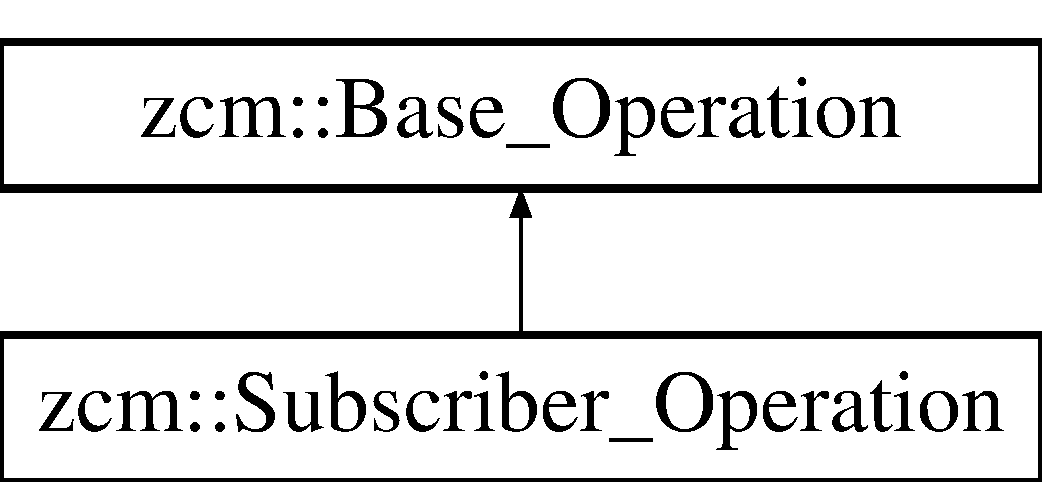
\includegraphics[height=2.000000cm]{classzcm_1_1Subscriber__Operation}
\end{center}
\end{figure}
\subsection*{Public Member Functions}
\begin{DoxyCompactItemize}
\item 
\hyperlink{classzcm_1_1Subscriber__Operation_aa0422263c6afea8bba3aa55b4c4e8c84}{Subscriber\+\_\+\+Operation} (std\+::string \hyperlink{classzcm_1_1Base__Operation_a2e2192550818d8f063fc7b2c76c5e21c}{name}, unsigned int \hyperlink{classzcm_1_1Base__Operation_a38af3bcc2578ef215772d595bf3fa358}{priority}, std\+::function$<$ void()$>$ \hyperlink{classzcm_1_1Subscriber__Operation_a5e3ca90f3ea6f1342d76f49363206e06}{operation\+\_\+function})
\begin{DoxyCompactList}\small\item\em Construct a subscriber operation. \end{DoxyCompactList}\item 
void \hyperlink{classzcm_1_1Subscriber__Operation_a2677079c7f3dd85cfc548427c1c101e6}{execute} ()
\begin{DoxyCompactList}\small\item\em \hyperlink{classzcm_1_1Subscriber}{Subscriber} operation function. \end{DoxyCompactList}\item 
std\+::string \hyperlink{classzcm_1_1Base__Operation_a46b6a3f23e18bc35425ec2dab80c849f}{get\+\_\+name} ()
\begin{DoxyCompactList}\small\item\em Return the operation name. \end{DoxyCompactList}\item 
unsigned int \hyperlink{classzcm_1_1Base__Operation_a3b15b35c31ed173d2abb193e9fba32ef}{get\+\_\+priority} () const 
\begin{DoxyCompactList}\small\item\em Return the operation priority. \end{DoxyCompactList}\end{DoxyCompactItemize}
\subsection*{Private Attributes}
\begin{DoxyCompactItemize}
\item 
std\+::function$<$ void()$>$ \hyperlink{classzcm_1_1Subscriber__Operation_a5e3ca90f3ea6f1342d76f49363206e06}{operation\+\_\+function}
\begin{DoxyCompactList}\small\item\em \hyperlink{classzcm_1_1Subscriber}{Subscriber} Operation Function. \end{DoxyCompactList}\end{DoxyCompactItemize}


\subsection{Detailed Description}
\hyperlink{classzcm_1_1Subscriber}{Subscriber} Operation class. 

\subsection{Constructor \& Destructor Documentation}
\index{zcm\+::\+Subscriber\+\_\+\+Operation@{zcm\+::\+Subscriber\+\_\+\+Operation}!Subscriber\+\_\+\+Operation@{Subscriber\+\_\+\+Operation}}
\index{Subscriber\+\_\+\+Operation@{Subscriber\+\_\+\+Operation}!zcm\+::\+Subscriber\+\_\+\+Operation@{zcm\+::\+Subscriber\+\_\+\+Operation}}
\subsubsection[{\texorpdfstring{Subscriber\+\_\+\+Operation(std\+::string name, unsigned int priority, std\+::function$<$ void()$>$ operation\+\_\+function)}{Subscriber_Operation(std::string name, unsigned int priority, std::function< void()> operation_function)}}]{\setlength{\rightskip}{0pt plus 5cm}zcm\+::\+Subscriber\+\_\+\+Operation\+::\+Subscriber\+\_\+\+Operation (
\begin{DoxyParamCaption}
\item[{std\+::string}]{name, }
\item[{unsigned int}]{priority, }
\item[{std\+::function$<$ void()$>$}]{operation\+\_\+function}
\end{DoxyParamCaption}
)\hspace{0.3cm}{\ttfamily [inline]}}\hypertarget{classzcm_1_1Subscriber__Operation_aa0422263c6afea8bba3aa55b4c4e8c84}{}\label{classzcm_1_1Subscriber__Operation_aa0422263c6afea8bba3aa55b4c4e8c84}


Construct a subscriber operation. 


\begin{DoxyParams}[1]{Parameters}
\mbox{\tt in}  & {\em name} & Name of the operation \\
\hline
\mbox{\tt in}  & {\em priority} & Priority of the operation \\
\hline
\mbox{\tt in}  & {\em operation\+\_\+function} & \hyperlink{classzcm_1_1Subscriber}{Subscriber} function \\
\hline
\end{DoxyParams}


\subsection{Member Function Documentation}
\index{zcm\+::\+Subscriber\+\_\+\+Operation@{zcm\+::\+Subscriber\+\_\+\+Operation}!execute@{execute}}
\index{execute@{execute}!zcm\+::\+Subscriber\+\_\+\+Operation@{zcm\+::\+Subscriber\+\_\+\+Operation}}
\subsubsection[{\texorpdfstring{execute()}{execute()}}]{\setlength{\rightskip}{0pt plus 5cm}void zcm\+::\+Subscriber\+\_\+\+Operation\+::execute (
\begin{DoxyParamCaption}
{}
\end{DoxyParamCaption}
)\hspace{0.3cm}{\ttfamily [virtual]}}\hypertarget{classzcm_1_1Subscriber__Operation_a2677079c7f3dd85cfc548427c1c101e6}{}\label{classzcm_1_1Subscriber__Operation_a2677079c7f3dd85cfc548427c1c101e6}


\hyperlink{classzcm_1_1Subscriber}{Subscriber} operation function. 



Reimplemented from \hyperlink{classzcm_1_1Base__Operation_a58cb533edd6e6f220d2d1c260fbddca4}{zcm\+::\+Base\+\_\+\+Operation}.

\index{zcm\+::\+Subscriber\+\_\+\+Operation@{zcm\+::\+Subscriber\+\_\+\+Operation}!get\+\_\+name@{get\+\_\+name}}
\index{get\+\_\+name@{get\+\_\+name}!zcm\+::\+Subscriber\+\_\+\+Operation@{zcm\+::\+Subscriber\+\_\+\+Operation}}
\subsubsection[{\texorpdfstring{get\+\_\+name()}{get_name()}}]{\setlength{\rightskip}{0pt plus 5cm}std\+::string zcm\+::\+Base\+\_\+\+Operation\+::get\+\_\+name (
\begin{DoxyParamCaption}
{}
\end{DoxyParamCaption}
)\hspace{0.3cm}{\ttfamily [inherited]}}\hypertarget{classzcm_1_1Base__Operation_a46b6a3f23e18bc35425ec2dab80c849f}{}\label{classzcm_1_1Base__Operation_a46b6a3f23e18bc35425ec2dab80c849f}


Return the operation name. 

\begin{DoxyReturn}{Returns}
Name of the operation 
\end{DoxyReturn}
\index{zcm\+::\+Subscriber\+\_\+\+Operation@{zcm\+::\+Subscriber\+\_\+\+Operation}!get\+\_\+priority@{get\+\_\+priority}}
\index{get\+\_\+priority@{get\+\_\+priority}!zcm\+::\+Subscriber\+\_\+\+Operation@{zcm\+::\+Subscriber\+\_\+\+Operation}}
\subsubsection[{\texorpdfstring{get\+\_\+priority() const }{get_priority() const }}]{\setlength{\rightskip}{0pt plus 5cm}unsigned int zcm\+::\+Base\+\_\+\+Operation\+::get\+\_\+priority (
\begin{DoxyParamCaption}
{}
\end{DoxyParamCaption}
) const\hspace{0.3cm}{\ttfamily [inherited]}}\hypertarget{classzcm_1_1Base__Operation_a3b15b35c31ed173d2abb193e9fba32ef}{}\label{classzcm_1_1Base__Operation_a3b15b35c31ed173d2abb193e9fba32ef}


Return the operation priority. 

\begin{DoxyReturn}{Returns}
Priority of the operation 
\end{DoxyReturn}


\subsection{Member Data Documentation}
\index{zcm\+::\+Subscriber\+\_\+\+Operation@{zcm\+::\+Subscriber\+\_\+\+Operation}!operation\+\_\+function@{operation\+\_\+function}}
\index{operation\+\_\+function@{operation\+\_\+function}!zcm\+::\+Subscriber\+\_\+\+Operation@{zcm\+::\+Subscriber\+\_\+\+Operation}}
\subsubsection[{\texorpdfstring{operation\+\_\+function}{operation_function}}]{\setlength{\rightskip}{0pt plus 5cm}std\+::function$<$void()$>$ zcm\+::\+Subscriber\+\_\+\+Operation\+::operation\+\_\+function\hspace{0.3cm}{\ttfamily [private]}}\hypertarget{classzcm_1_1Subscriber__Operation_a5e3ca90f3ea6f1342d76f49363206e06}{}\label{classzcm_1_1Subscriber__Operation_a5e3ca90f3ea6f1342d76f49363206e06}


\hyperlink{classzcm_1_1Subscriber}{Subscriber} Operation Function. 



The documentation for this class was generated from the following files\+:\begin{DoxyCompactItemize}
\item 
/home/pranav/\+Repositories/zcm/include/\hyperlink{operation__types_8hpp}{operation\+\_\+types.\+hpp}\item 
/home/pranav/\+Repositories/zcm/src/\hyperlink{operation__types_8cpp}{operation\+\_\+types.\+cpp}\end{DoxyCompactItemize}

\hypertarget{classzcm_1_1Timer}{}\section{zcm\+:\+:Timer Class Reference}
\label{classzcm_1_1Timer}\index{zcm\+::\+Timer@{zcm\+::\+Timer}}


\hyperlink{classzcm_1_1Timer}{Timer} class.  




{\ttfamily \#include $<$timer.\+hpp$>$}

\subsection*{Public Member Functions}
\begin{DoxyCompactItemize}
\item 
\hyperlink{classzcm_1_1Timer_a1283d5045e825f0f07c1cf3117eb1904}{Timer} (std\+::string \hyperlink{classzcm_1_1Timer_abfd2bb014b496ce2eda5a5837e9275f1}{name}, unsigned int \hyperlink{classzcm_1_1Timer_a722f6390254d106117d8e1545b6092ab}{priority}, long long \hyperlink{classzcm_1_1Timer_a36c7498a7ad5706ceca83429e6c1759c}{period}, std\+::function$<$ void()$>$ \hyperlink{classzcm_1_1Timer_a07f820c2d67029b83547bbfd77fc3690}{operation\+\_\+function}, \hyperlink{classzcm_1_1Operation__Queue}{Operation\+\_\+\+Queue} $\ast$\hyperlink{classzcm_1_1Timer_a9f2ce34fb9230c4251355fde956b7220}{operation\+\_\+queue\+\_\+ptr})
\begin{DoxyCompactList}\small\item\em Construct a timer. \end{DoxyCompactList}\item 
void \hyperlink{classzcm_1_1Timer_a4baed4e019656ed2612aaa0374cc0fa9}{operation} ()
\begin{DoxyCompactList}\small\item\em \hyperlink{classzcm_1_1Timer}{Timer} thread function Behavior\+: (1) Wait for timer expiry (2) Create a \hyperlink{classzcm_1_1Timer__Operation}{Timer\+\_\+\+Operation} (3) Enqueue onto operation\+\_\+queue (4) Goto step (1) \end{DoxyCompactList}\item 
std\+::string \hyperlink{classzcm_1_1Timer_a4a4aaf655539dec8ca7e747e230f8655}{get\+\_\+name} ()
\begin{DoxyCompactList}\small\item\em Get the timer name. \end{DoxyCompactList}\item 
unsigned int \hyperlink{classzcm_1_1Timer_a468548503d67c3e3872cf85d86cb26ba}{get\+\_\+priority} ()
\begin{DoxyCompactList}\small\item\em Get the timer priority. \end{DoxyCompactList}\item 
void \hyperlink{classzcm_1_1Timer_a70d8498a7fcfacc90a4510baa55682ef}{change\+\_\+period} (long long new\+\_\+period)
\begin{DoxyCompactList}\small\item\em Change the timer period. \end{DoxyCompactList}\item 
void \hyperlink{classzcm_1_1Timer_ace30a8e8155fcacf5ea8b7eee796b02b}{rebind\+\_\+operation\+\_\+function} (std\+::function$<$ void()$>$ new\+\_\+operation\+\_\+function)
\begin{DoxyCompactList}\small\item\em Rebind the timer operation function. \end{DoxyCompactList}\item 
std\+::thread \hyperlink{classzcm_1_1Timer_a05e22ac74661a4891f610e0c0d364ca7}{spawn} ()
\begin{DoxyCompactList}\small\item\em Spawn a new thread for the timer. \end{DoxyCompactList}\item 
void \hyperlink{classzcm_1_1Timer_a2a7ba9c6294a1a726844c71db962a280}{start} ()
\begin{DoxyCompactList}\small\item\em Start the timer thread. \end{DoxyCompactList}\end{DoxyCompactItemize}
\subsection*{Private Attributes}
\begin{DoxyCompactItemize}
\item 
std\+::string \hyperlink{classzcm_1_1Timer_abfd2bb014b496ce2eda5a5837e9275f1}{name}
\begin{DoxyCompactList}\small\item\em Name of the timer. \end{DoxyCompactList}\item 
unsigned int \hyperlink{classzcm_1_1Timer_a722f6390254d106117d8e1545b6092ab}{priority}
\begin{DoxyCompactList}\small\item\em Priority of the timer. \end{DoxyCompactList}\item 
std\+::chrono\+::duration$<$ long long, std\+::ratio$<$ 1, 1000000000 $>$ $>$ \hyperlink{classzcm_1_1Timer_a36c7498a7ad5706ceca83429e6c1759c}{period}
\begin{DoxyCompactList}\small\item\em Period of the timer. \end{DoxyCompactList}\item 
std\+::function$<$ void()$>$ \hyperlink{classzcm_1_1Timer_a07f820c2d67029b83547bbfd77fc3690}{operation\+\_\+function}
\begin{DoxyCompactList}\small\item\em Operation function bound to the timer. \end{DoxyCompactList}\item 
\hyperlink{classzcm_1_1Operation__Queue}{Operation\+\_\+\+Queue} $\ast$ \hyperlink{classzcm_1_1Timer_a9f2ce34fb9230c4251355fde956b7220}{operation\+\_\+queue\+\_\+ptr}
\begin{DoxyCompactList}\small\item\em Pointer to the operation queue. \end{DoxyCompactList}\item 
std\+::mutex \hyperlink{classzcm_1_1Timer_af9d6ce4df403e44b543241926ddcf41f}{period\+\_\+mutex}
\begin{DoxyCompactList}\small\item\em Mutex used to change the timer period at runtime. \end{DoxyCompactList}\item 
std\+::mutex \hyperlink{classzcm_1_1Timer_a987e7fd6128be8eac6a6a3d60c7ef9b3}{func\+\_\+mutex}
\begin{DoxyCompactList}\small\item\em Mutex used to change the operation\+\_\+function at runtime. \end{DoxyCompactList}\end{DoxyCompactItemize}


\subsection{Detailed Description}
\hyperlink{classzcm_1_1Timer}{Timer} class. 

\subsection{Constructor \& Destructor Documentation}
\index{zcm\+::\+Timer@{zcm\+::\+Timer}!Timer@{Timer}}
\index{Timer@{Timer}!zcm\+::\+Timer@{zcm\+::\+Timer}}
\subsubsection[{\texorpdfstring{Timer(std\+::string name, unsigned int priority, long long period, std\+::function$<$ void()$>$ operation\+\_\+function, Operation\+\_\+\+Queue $\ast$operation\+\_\+queue\+\_\+ptr)}{Timer(std::string name, unsigned int priority, long long period, std::function< void()> operation_function, Operation_Queue *operation_queue_ptr)}}]{\setlength{\rightskip}{0pt plus 5cm}zcm\+::\+Timer\+::\+Timer (
\begin{DoxyParamCaption}
\item[{std\+::string}]{name, }
\item[{unsigned int}]{priority, }
\item[{long long}]{period, }
\item[{std\+::function$<$ void()$>$}]{operation\+\_\+function, }
\item[{{\bf Operation\+\_\+\+Queue} $\ast$}]{operation\+\_\+queue\+\_\+ptr}
\end{DoxyParamCaption}
)}\hypertarget{classzcm_1_1Timer_a1283d5045e825f0f07c1cf3117eb1904}{}\label{classzcm_1_1Timer_a1283d5045e825f0f07c1cf3117eb1904}


Construct a timer. 


\begin{DoxyParams}[1]{Parameters}
\mbox{\tt in}  & {\em name} & Name of the timer \\
\hline
\mbox{\tt in}  & {\em priority} & Priority of the timer \\
\hline
\mbox{\tt in}  & {\em period} & Period of the timer in nanoseconds \\
\hline
\mbox{\tt in}  & {\em operation\+\_\+function} & Operation to which the timer is bound \\
\hline
\mbox{\tt in}  & {\em operation\+\_\+queue\+\_\+ptr} & Pointer to the operation\+\_\+queue \\
\hline
\end{DoxyParams}


\subsection{Member Function Documentation}
\index{zcm\+::\+Timer@{zcm\+::\+Timer}!change\+\_\+period@{change\+\_\+period}}
\index{change\+\_\+period@{change\+\_\+period}!zcm\+::\+Timer@{zcm\+::\+Timer}}
\subsubsection[{\texorpdfstring{change\+\_\+period(long long new\+\_\+period)}{change_period(long long new_period)}}]{\setlength{\rightskip}{0pt plus 5cm}void zcm\+::\+Timer\+::change\+\_\+period (
\begin{DoxyParamCaption}
\item[{long long}]{new\+\_\+period}
\end{DoxyParamCaption}
)}\hypertarget{classzcm_1_1Timer_a70d8498a7fcfacc90a4510baa55682ef}{}\label{classzcm_1_1Timer_a70d8498a7fcfacc90a4510baa55682ef}


Change the timer period. 


\begin{DoxyParams}[1]{Parameters}
\mbox{\tt in}  & {\em new\+\_\+period} & New timer period in nanoseconds \\
\hline
\end{DoxyParams}
\index{zcm\+::\+Timer@{zcm\+::\+Timer}!get\+\_\+name@{get\+\_\+name}}
\index{get\+\_\+name@{get\+\_\+name}!zcm\+::\+Timer@{zcm\+::\+Timer}}
\subsubsection[{\texorpdfstring{get\+\_\+name()}{get_name()}}]{\setlength{\rightskip}{0pt plus 5cm}std\+::string zcm\+::\+Timer\+::get\+\_\+name (
\begin{DoxyParamCaption}
{}
\end{DoxyParamCaption}
)}\hypertarget{classzcm_1_1Timer_a4a4aaf655539dec8ca7e747e230f8655}{}\label{classzcm_1_1Timer_a4a4aaf655539dec8ca7e747e230f8655}


Get the timer name. 

\begin{DoxyReturn}{Returns}
\hyperlink{classzcm_1_1Timer}{Timer} name 
\end{DoxyReturn}
\index{zcm\+::\+Timer@{zcm\+::\+Timer}!get\+\_\+priority@{get\+\_\+priority}}
\index{get\+\_\+priority@{get\+\_\+priority}!zcm\+::\+Timer@{zcm\+::\+Timer}}
\subsubsection[{\texorpdfstring{get\+\_\+priority()}{get_priority()}}]{\setlength{\rightskip}{0pt plus 5cm}unsigned int zcm\+::\+Timer\+::get\+\_\+priority (
\begin{DoxyParamCaption}
{}
\end{DoxyParamCaption}
)}\hypertarget{classzcm_1_1Timer_a468548503d67c3e3872cf85d86cb26ba}{}\label{classzcm_1_1Timer_a468548503d67c3e3872cf85d86cb26ba}


Get the timer priority. 

\begin{DoxyReturn}{Returns}
\hyperlink{classzcm_1_1Timer}{Timer} priority 
\end{DoxyReturn}
\index{zcm\+::\+Timer@{zcm\+::\+Timer}!operation@{operation}}
\index{operation@{operation}!zcm\+::\+Timer@{zcm\+::\+Timer}}
\subsubsection[{\texorpdfstring{operation()}{operation()}}]{\setlength{\rightskip}{0pt plus 5cm}void zcm\+::\+Timer\+::operation (
\begin{DoxyParamCaption}
{}
\end{DoxyParamCaption}
)}\hypertarget{classzcm_1_1Timer_a4baed4e019656ed2612aaa0374cc0fa9}{}\label{classzcm_1_1Timer_a4baed4e019656ed2612aaa0374cc0fa9}


\hyperlink{classzcm_1_1Timer}{Timer} thread function Behavior\+: (1) Wait for timer expiry (2) Create a \hyperlink{classzcm_1_1Timer__Operation}{Timer\+\_\+\+Operation} (3) Enqueue onto operation\+\_\+queue (4) Goto step (1) 

\index{zcm\+::\+Timer@{zcm\+::\+Timer}!rebind\+\_\+operation\+\_\+function@{rebind\+\_\+operation\+\_\+function}}
\index{rebind\+\_\+operation\+\_\+function@{rebind\+\_\+operation\+\_\+function}!zcm\+::\+Timer@{zcm\+::\+Timer}}
\subsubsection[{\texorpdfstring{rebind\+\_\+operation\+\_\+function(std\+::function$<$ void()$>$ new\+\_\+operation\+\_\+function)}{rebind_operation_function(std::function< void()> new_operation_function)}}]{\setlength{\rightskip}{0pt plus 5cm}void zcm\+::\+Timer\+::rebind\+\_\+operation\+\_\+function (
\begin{DoxyParamCaption}
\item[{std\+::function$<$ void()$>$}]{new\+\_\+operation\+\_\+function}
\end{DoxyParamCaption}
)}\hypertarget{classzcm_1_1Timer_ace30a8e8155fcacf5ea8b7eee796b02b}{}\label{classzcm_1_1Timer_ace30a8e8155fcacf5ea8b7eee796b02b}


Rebind the timer operation function. 


\begin{DoxyParams}[1]{Parameters}
\mbox{\tt in}  & {\em new\+\_\+operation\+\_\+function} & New timer function to be handled upon expiry \\
\hline
\end{DoxyParams}
\index{zcm\+::\+Timer@{zcm\+::\+Timer}!spawn@{spawn}}
\index{spawn@{spawn}!zcm\+::\+Timer@{zcm\+::\+Timer}}
\subsubsection[{\texorpdfstring{spawn()}{spawn()}}]{\setlength{\rightskip}{0pt plus 5cm}std\+::thread zcm\+::\+Timer\+::spawn (
\begin{DoxyParamCaption}
{}
\end{DoxyParamCaption}
)}\hypertarget{classzcm_1_1Timer_a05e22ac74661a4891f610e0c0d364ca7}{}\label{classzcm_1_1Timer_a05e22ac74661a4891f610e0c0d364ca7}


Spawn a new thread for the timer. 

\begin{DoxyReturn}{Returns}
\hyperlink{classzcm_1_1Timer}{Timer} thread 
\end{DoxyReturn}
\index{zcm\+::\+Timer@{zcm\+::\+Timer}!start@{start}}
\index{start@{start}!zcm\+::\+Timer@{zcm\+::\+Timer}}
\subsubsection[{\texorpdfstring{start()}{start()}}]{\setlength{\rightskip}{0pt plus 5cm}void zcm\+::\+Timer\+::start (
\begin{DoxyParamCaption}
{}
\end{DoxyParamCaption}
)}\hypertarget{classzcm_1_1Timer_a2a7ba9c6294a1a726844c71db962a280}{}\label{classzcm_1_1Timer_a2a7ba9c6294a1a726844c71db962a280}


Start the timer thread. 



\subsection{Member Data Documentation}
\index{zcm\+::\+Timer@{zcm\+::\+Timer}!func\+\_\+mutex@{func\+\_\+mutex}}
\index{func\+\_\+mutex@{func\+\_\+mutex}!zcm\+::\+Timer@{zcm\+::\+Timer}}
\subsubsection[{\texorpdfstring{func\+\_\+mutex}{func_mutex}}]{\setlength{\rightskip}{0pt plus 5cm}std\+::mutex zcm\+::\+Timer\+::func\+\_\+mutex\hspace{0.3cm}{\ttfamily [private]}}\hypertarget{classzcm_1_1Timer_a987e7fd6128be8eac6a6a3d60c7ef9b3}{}\label{classzcm_1_1Timer_a987e7fd6128be8eac6a6a3d60c7ef9b3}


Mutex used to change the operation\+\_\+function at runtime. 

\index{zcm\+::\+Timer@{zcm\+::\+Timer}!name@{name}}
\index{name@{name}!zcm\+::\+Timer@{zcm\+::\+Timer}}
\subsubsection[{\texorpdfstring{name}{name}}]{\setlength{\rightskip}{0pt plus 5cm}std\+::string zcm\+::\+Timer\+::name\hspace{0.3cm}{\ttfamily [private]}}\hypertarget{classzcm_1_1Timer_abfd2bb014b496ce2eda5a5837e9275f1}{}\label{classzcm_1_1Timer_abfd2bb014b496ce2eda5a5837e9275f1}


Name of the timer. 

\index{zcm\+::\+Timer@{zcm\+::\+Timer}!operation\+\_\+function@{operation\+\_\+function}}
\index{operation\+\_\+function@{operation\+\_\+function}!zcm\+::\+Timer@{zcm\+::\+Timer}}
\subsubsection[{\texorpdfstring{operation\+\_\+function}{operation_function}}]{\setlength{\rightskip}{0pt plus 5cm}std\+::function$<$void()$>$ zcm\+::\+Timer\+::operation\+\_\+function\hspace{0.3cm}{\ttfamily [private]}}\hypertarget{classzcm_1_1Timer_a07f820c2d67029b83547bbfd77fc3690}{}\label{classzcm_1_1Timer_a07f820c2d67029b83547bbfd77fc3690}


Operation function bound to the timer. 

\index{zcm\+::\+Timer@{zcm\+::\+Timer}!operation\+\_\+queue\+\_\+ptr@{operation\+\_\+queue\+\_\+ptr}}
\index{operation\+\_\+queue\+\_\+ptr@{operation\+\_\+queue\+\_\+ptr}!zcm\+::\+Timer@{zcm\+::\+Timer}}
\subsubsection[{\texorpdfstring{operation\+\_\+queue\+\_\+ptr}{operation_queue_ptr}}]{\setlength{\rightskip}{0pt plus 5cm}{\bf Operation\+\_\+\+Queue}$\ast$ zcm\+::\+Timer\+::operation\+\_\+queue\+\_\+ptr\hspace{0.3cm}{\ttfamily [private]}}\hypertarget{classzcm_1_1Timer_a9f2ce34fb9230c4251355fde956b7220}{}\label{classzcm_1_1Timer_a9f2ce34fb9230c4251355fde956b7220}


Pointer to the operation queue. 

\index{zcm\+::\+Timer@{zcm\+::\+Timer}!period@{period}}
\index{period@{period}!zcm\+::\+Timer@{zcm\+::\+Timer}}
\subsubsection[{\texorpdfstring{period}{period}}]{\setlength{\rightskip}{0pt plus 5cm}std\+::chrono\+::duration$<$long long, std\+::ratio$<$1, 1000000000$>$ $>$ zcm\+::\+Timer\+::period\hspace{0.3cm}{\ttfamily [private]}}\hypertarget{classzcm_1_1Timer_a36c7498a7ad5706ceca83429e6c1759c}{}\label{classzcm_1_1Timer_a36c7498a7ad5706ceca83429e6c1759c}


Period of the timer. 

\index{zcm\+::\+Timer@{zcm\+::\+Timer}!period\+\_\+mutex@{period\+\_\+mutex}}
\index{period\+\_\+mutex@{period\+\_\+mutex}!zcm\+::\+Timer@{zcm\+::\+Timer}}
\subsubsection[{\texorpdfstring{period\+\_\+mutex}{period_mutex}}]{\setlength{\rightskip}{0pt plus 5cm}std\+::mutex zcm\+::\+Timer\+::period\+\_\+mutex\hspace{0.3cm}{\ttfamily [private]}}\hypertarget{classzcm_1_1Timer_af9d6ce4df403e44b543241926ddcf41f}{}\label{classzcm_1_1Timer_af9d6ce4df403e44b543241926ddcf41f}


Mutex used to change the timer period at runtime. 

\index{zcm\+::\+Timer@{zcm\+::\+Timer}!priority@{priority}}
\index{priority@{priority}!zcm\+::\+Timer@{zcm\+::\+Timer}}
\subsubsection[{\texorpdfstring{priority}{priority}}]{\setlength{\rightskip}{0pt plus 5cm}unsigned int zcm\+::\+Timer\+::priority\hspace{0.3cm}{\ttfamily [private]}}\hypertarget{classzcm_1_1Timer_a722f6390254d106117d8e1545b6092ab}{}\label{classzcm_1_1Timer_a722f6390254d106117d8e1545b6092ab}


Priority of the timer. 



The documentation for this class was generated from the following files\+:\begin{DoxyCompactItemize}
\item 
/home/pranav/\+Repositories/zcm/include/\hyperlink{timer_8hpp}{timer.\+hpp}\item 
/home/pranav/\+Repositories/zcm/src/\hyperlink{timer_8cpp}{timer.\+cpp}\end{DoxyCompactItemize}

\hypertarget{classzcm_1_1Timer__Operation}{}\section{zcm\+:\+:Timer\+\_\+\+Operation Class Reference}
\label{classzcm_1_1Timer__Operation}\index{zcm\+::\+Timer\+\_\+\+Operation@{zcm\+::\+Timer\+\_\+\+Operation}}


\hyperlink{classzcm_1_1Timer}{Timer} Operation class.  




{\ttfamily \#include $<$operation\+\_\+types.\+hpp$>$}

Inheritance diagram for zcm\+:\+:Timer\+\_\+\+Operation\+:\begin{figure}[H]
\begin{center}
\leavevmode
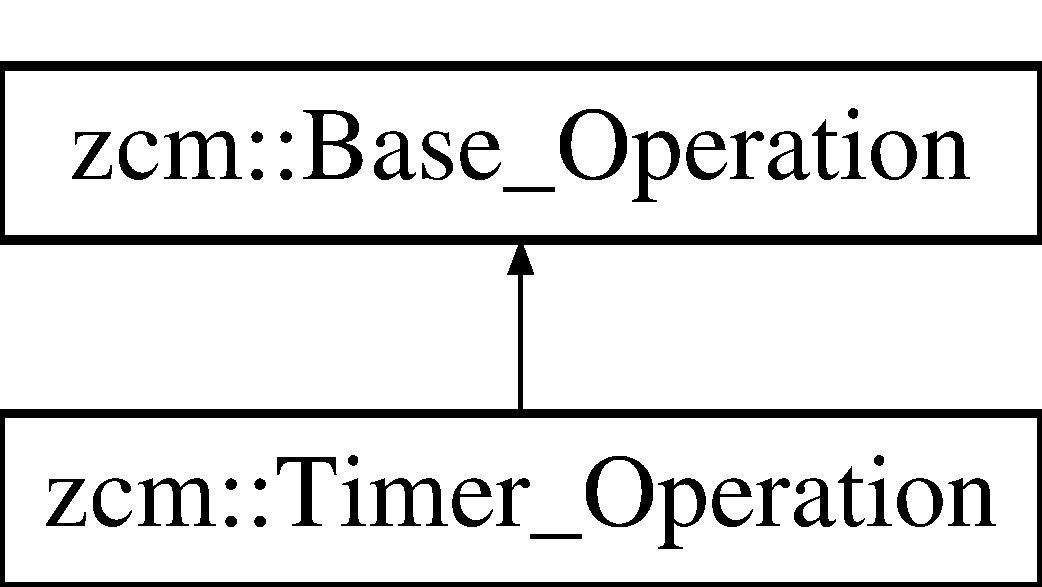
\includegraphics[height=2.000000cm]{classzcm_1_1Timer__Operation}
\end{center}
\end{figure}
\subsection*{Public Member Functions}
\begin{DoxyCompactItemize}
\item 
\hyperlink{classzcm_1_1Timer__Operation_aa578839e1aaf755f92170f20865a5740}{Timer\+\_\+\+Operation} (std\+::string \hyperlink{classzcm_1_1Base__Operation_a2e2192550818d8f063fc7b2c76c5e21c}{name}, unsigned int \hyperlink{classzcm_1_1Base__Operation_a38af3bcc2578ef215772d595bf3fa358}{priority}, std\+::function$<$ void()$>$ \hyperlink{classzcm_1_1Timer__Operation_a492e0ec6be1dfa846bbc83d9e5dea9b0}{operation\+\_\+function})
\begin{DoxyCompactList}\small\item\em Construct a timer operation. \end{DoxyCompactList}\item 
void \hyperlink{classzcm_1_1Timer__Operation_a3693312c4d4d106d0894bb35094efda7}{execute} ()
\begin{DoxyCompactList}\small\item\em \hyperlink{classzcm_1_1Timer}{Timer} operation function. \end{DoxyCompactList}\item 
std\+::string \hyperlink{classzcm_1_1Base__Operation_a46b6a3f23e18bc35425ec2dab80c849f}{get\+\_\+name} ()
\begin{DoxyCompactList}\small\item\em Return the operation name. \end{DoxyCompactList}\item 
unsigned int \hyperlink{classzcm_1_1Base__Operation_a3b15b35c31ed173d2abb193e9fba32ef}{get\+\_\+priority} () const 
\begin{DoxyCompactList}\small\item\em Return the operation priority. \end{DoxyCompactList}\end{DoxyCompactItemize}
\subsection*{Private Attributes}
\begin{DoxyCompactItemize}
\item 
std\+::function$<$ void()$>$ \hyperlink{classzcm_1_1Timer__Operation_a492e0ec6be1dfa846bbc83d9e5dea9b0}{operation\+\_\+function}
\begin{DoxyCompactList}\small\item\em \hyperlink{classzcm_1_1Timer}{Timer} operation function. \end{DoxyCompactList}\end{DoxyCompactItemize}


\subsection{Detailed Description}
\hyperlink{classzcm_1_1Timer}{Timer} Operation class. 

\subsection{Constructor \& Destructor Documentation}
\index{zcm\+::\+Timer\+\_\+\+Operation@{zcm\+::\+Timer\+\_\+\+Operation}!Timer\+\_\+\+Operation@{Timer\+\_\+\+Operation}}
\index{Timer\+\_\+\+Operation@{Timer\+\_\+\+Operation}!zcm\+::\+Timer\+\_\+\+Operation@{zcm\+::\+Timer\+\_\+\+Operation}}
\subsubsection[{\texorpdfstring{Timer\+\_\+\+Operation(std\+::string name, unsigned int priority, std\+::function$<$ void()$>$ operation\+\_\+function)}{Timer_Operation(std::string name, unsigned int priority, std::function< void()> operation_function)}}]{\setlength{\rightskip}{0pt plus 5cm}zcm\+::\+Timer\+\_\+\+Operation\+::\+Timer\+\_\+\+Operation (
\begin{DoxyParamCaption}
\item[{std\+::string}]{name, }
\item[{unsigned int}]{priority, }
\item[{std\+::function$<$ void()$>$}]{operation\+\_\+function}
\end{DoxyParamCaption}
)\hspace{0.3cm}{\ttfamily [inline]}}\hypertarget{classzcm_1_1Timer__Operation_aa578839e1aaf755f92170f20865a5740}{}\label{classzcm_1_1Timer__Operation_aa578839e1aaf755f92170f20865a5740}


Construct a timer operation. 


\begin{DoxyParams}[1]{Parameters}
\mbox{\tt in}  & {\em name} & Name of the operation \\
\hline
\mbox{\tt in}  & {\em priority} & Priority of the operation \\
\hline
\mbox{\tt in}  & {\em operation\+\_\+function} & \hyperlink{classzcm_1_1Timer}{Timer} function \\
\hline
\end{DoxyParams}


\subsection{Member Function Documentation}
\index{zcm\+::\+Timer\+\_\+\+Operation@{zcm\+::\+Timer\+\_\+\+Operation}!execute@{execute}}
\index{execute@{execute}!zcm\+::\+Timer\+\_\+\+Operation@{zcm\+::\+Timer\+\_\+\+Operation}}
\subsubsection[{\texorpdfstring{execute()}{execute()}}]{\setlength{\rightskip}{0pt plus 5cm}void zcm\+::\+Timer\+\_\+\+Operation\+::execute (
\begin{DoxyParamCaption}
{}
\end{DoxyParamCaption}
)\hspace{0.3cm}{\ttfamily [virtual]}}\hypertarget{classzcm_1_1Timer__Operation_a3693312c4d4d106d0894bb35094efda7}{}\label{classzcm_1_1Timer__Operation_a3693312c4d4d106d0894bb35094efda7}


\hyperlink{classzcm_1_1Timer}{Timer} operation function. 



Reimplemented from \hyperlink{classzcm_1_1Base__Operation_a58cb533edd6e6f220d2d1c260fbddca4}{zcm\+::\+Base\+\_\+\+Operation}.

\index{zcm\+::\+Timer\+\_\+\+Operation@{zcm\+::\+Timer\+\_\+\+Operation}!get\+\_\+name@{get\+\_\+name}}
\index{get\+\_\+name@{get\+\_\+name}!zcm\+::\+Timer\+\_\+\+Operation@{zcm\+::\+Timer\+\_\+\+Operation}}
\subsubsection[{\texorpdfstring{get\+\_\+name()}{get_name()}}]{\setlength{\rightskip}{0pt plus 5cm}std\+::string zcm\+::\+Base\+\_\+\+Operation\+::get\+\_\+name (
\begin{DoxyParamCaption}
{}
\end{DoxyParamCaption}
)\hspace{0.3cm}{\ttfamily [inherited]}}\hypertarget{classzcm_1_1Base__Operation_a46b6a3f23e18bc35425ec2dab80c849f}{}\label{classzcm_1_1Base__Operation_a46b6a3f23e18bc35425ec2dab80c849f}


Return the operation name. 

\begin{DoxyReturn}{Returns}
Name of the operation 
\end{DoxyReturn}
\index{zcm\+::\+Timer\+\_\+\+Operation@{zcm\+::\+Timer\+\_\+\+Operation}!get\+\_\+priority@{get\+\_\+priority}}
\index{get\+\_\+priority@{get\+\_\+priority}!zcm\+::\+Timer\+\_\+\+Operation@{zcm\+::\+Timer\+\_\+\+Operation}}
\subsubsection[{\texorpdfstring{get\+\_\+priority() const }{get_priority() const }}]{\setlength{\rightskip}{0pt plus 5cm}unsigned int zcm\+::\+Base\+\_\+\+Operation\+::get\+\_\+priority (
\begin{DoxyParamCaption}
{}
\end{DoxyParamCaption}
) const\hspace{0.3cm}{\ttfamily [inherited]}}\hypertarget{classzcm_1_1Base__Operation_a3b15b35c31ed173d2abb193e9fba32ef}{}\label{classzcm_1_1Base__Operation_a3b15b35c31ed173d2abb193e9fba32ef}


Return the operation priority. 

\begin{DoxyReturn}{Returns}
Priority of the operation 
\end{DoxyReturn}


\subsection{Member Data Documentation}
\index{zcm\+::\+Timer\+\_\+\+Operation@{zcm\+::\+Timer\+\_\+\+Operation}!operation\+\_\+function@{operation\+\_\+function}}
\index{operation\+\_\+function@{operation\+\_\+function}!zcm\+::\+Timer\+\_\+\+Operation@{zcm\+::\+Timer\+\_\+\+Operation}}
\subsubsection[{\texorpdfstring{operation\+\_\+function}{operation_function}}]{\setlength{\rightskip}{0pt plus 5cm}std\+::function$<$void()$>$ zcm\+::\+Timer\+\_\+\+Operation\+::operation\+\_\+function\hspace{0.3cm}{\ttfamily [private]}}\hypertarget{classzcm_1_1Timer__Operation_a492e0ec6be1dfa846bbc83d9e5dea9b0}{}\label{classzcm_1_1Timer__Operation_a492e0ec6be1dfa846bbc83d9e5dea9b0}


\hyperlink{classzcm_1_1Timer}{Timer} operation function. 



The documentation for this class was generated from the following files\+:\begin{DoxyCompactItemize}
\item 
/home/pranav/\+Repositories/zcm/include/\hyperlink{operation__types_8hpp}{operation\+\_\+types.\+hpp}\item 
/home/pranav/\+Repositories/zcm/src/\hyperlink{operation__types_8cpp}{operation\+\_\+types.\+cpp}\end{DoxyCompactItemize}

\hypertarget{classJson_1_1OurReader_1_1Token}{}\section{Json\+:\+:Our\+Reader\+:\+:Token Class Reference}
\label{classJson_1_1OurReader_1_1Token}\index{Json\+::\+Our\+Reader\+::\+Token@{Json\+::\+Our\+Reader\+::\+Token}}
\subsection*{Public Attributes}
\begin{DoxyCompactItemize}
\item 
\hyperlink{classJson_1_1OurReader_a15116f7276ddf1e7a2cc3cbefa884dcc}{Token\+Type} \hyperlink{classJson_1_1OurReader_1_1Token_abe7d858530396fa7e1293f7a579880ed}{type\+\_\+}
\item 
\hyperlink{classJson_1_1OurReader_a1bdc7bbc52ba87cae6b19746f2ee0189}{Location} \hyperlink{classJson_1_1OurReader_1_1Token_aedf68bb00eaaa9d3c22b9825999602ac}{start\+\_\+}
\item 
\hyperlink{classJson_1_1OurReader_a1bdc7bbc52ba87cae6b19746f2ee0189}{Location} \hyperlink{classJson_1_1OurReader_1_1Token_a67d2071638add857528579ae3791eccc}{end\+\_\+}
\end{DoxyCompactItemize}


\subsection{Member Data Documentation}
\index{Json\+::\+Our\+Reader\+::\+Token@{Json\+::\+Our\+Reader\+::\+Token}!end\+\_\+@{end\+\_\+}}
\index{end\+\_\+@{end\+\_\+}!Json\+::\+Our\+Reader\+::\+Token@{Json\+::\+Our\+Reader\+::\+Token}}
\subsubsection[{\texorpdfstring{end\+\_\+}{end_}}]{\setlength{\rightskip}{0pt plus 5cm}{\bf Location} Json\+::\+Our\+Reader\+::\+Token\+::end\+\_\+}\hypertarget{classJson_1_1OurReader_1_1Token_a67d2071638add857528579ae3791eccc}{}\label{classJson_1_1OurReader_1_1Token_a67d2071638add857528579ae3791eccc}
\index{Json\+::\+Our\+Reader\+::\+Token@{Json\+::\+Our\+Reader\+::\+Token}!start\+\_\+@{start\+\_\+}}
\index{start\+\_\+@{start\+\_\+}!Json\+::\+Our\+Reader\+::\+Token@{Json\+::\+Our\+Reader\+::\+Token}}
\subsubsection[{\texorpdfstring{start\+\_\+}{start_}}]{\setlength{\rightskip}{0pt plus 5cm}{\bf Location} Json\+::\+Our\+Reader\+::\+Token\+::start\+\_\+}\hypertarget{classJson_1_1OurReader_1_1Token_aedf68bb00eaaa9d3c22b9825999602ac}{}\label{classJson_1_1OurReader_1_1Token_aedf68bb00eaaa9d3c22b9825999602ac}
\index{Json\+::\+Our\+Reader\+::\+Token@{Json\+::\+Our\+Reader\+::\+Token}!type\+\_\+@{type\+\_\+}}
\index{type\+\_\+@{type\+\_\+}!Json\+::\+Our\+Reader\+::\+Token@{Json\+::\+Our\+Reader\+::\+Token}}
\subsubsection[{\texorpdfstring{type\+\_\+}{type_}}]{\setlength{\rightskip}{0pt plus 5cm}{\bf Token\+Type} Json\+::\+Our\+Reader\+::\+Token\+::type\+\_\+}\hypertarget{classJson_1_1OurReader_1_1Token_abe7d858530396fa7e1293f7a579880ed}{}\label{classJson_1_1OurReader_1_1Token_abe7d858530396fa7e1293f7a579880ed}


The documentation for this class was generated from the following file\+:\begin{DoxyCompactItemize}
\item 
/home/pranav/\+Repositories/zcm/src/\hyperlink{json_8cpp}{json.\+cpp}\end{DoxyCompactItemize}

\hypertarget{classJson_1_1Reader_1_1Token}{}\section{Json\+:\+:Reader\+:\+:Token Class Reference}
\label{classJson_1_1Reader_1_1Token}\index{Json\+::\+Reader\+::\+Token@{Json\+::\+Reader\+::\+Token}}
\subsection*{Public Attributes}
\begin{DoxyCompactItemize}
\item 
\hyperlink{classJson_1_1Reader_aa35e6ab574dc399a0a645ad98ed66bc9}{Token\+Type} \hyperlink{classJson_1_1Reader_1_1Token_aa0f06d0105ec3d8cb42427c66b991bad}{type\+\_\+}
\item 
\hyperlink{classJson_1_1Reader_a46795b5b272bf79a7730e406cb96375a}{Location} \hyperlink{classJson_1_1Reader_1_1Token_aff87d677b9ac4b52542a00b0d6673249}{start\+\_\+}
\item 
\hyperlink{classJson_1_1Reader_a46795b5b272bf79a7730e406cb96375a}{Location} \hyperlink{classJson_1_1Reader_1_1Token_a7d3bc0fa40097f435d184be4b1fd5ae1}{end\+\_\+}
\end{DoxyCompactItemize}


\subsection{Member Data Documentation}
\index{Json\+::\+Reader\+::\+Token@{Json\+::\+Reader\+::\+Token}!end\+\_\+@{end\+\_\+}}
\index{end\+\_\+@{end\+\_\+}!Json\+::\+Reader\+::\+Token@{Json\+::\+Reader\+::\+Token}}
\subsubsection[{\texorpdfstring{end\+\_\+}{end_}}]{\setlength{\rightskip}{0pt plus 5cm}{\bf Location} Json\+::\+Reader\+::\+Token\+::end\+\_\+}\hypertarget{classJson_1_1Reader_1_1Token_a7d3bc0fa40097f435d184be4b1fd5ae1}{}\label{classJson_1_1Reader_1_1Token_a7d3bc0fa40097f435d184be4b1fd5ae1}
\index{Json\+::\+Reader\+::\+Token@{Json\+::\+Reader\+::\+Token}!start\+\_\+@{start\+\_\+}}
\index{start\+\_\+@{start\+\_\+}!Json\+::\+Reader\+::\+Token@{Json\+::\+Reader\+::\+Token}}
\subsubsection[{\texorpdfstring{start\+\_\+}{start_}}]{\setlength{\rightskip}{0pt plus 5cm}{\bf Location} Json\+::\+Reader\+::\+Token\+::start\+\_\+}\hypertarget{classJson_1_1Reader_1_1Token_aff87d677b9ac4b52542a00b0d6673249}{}\label{classJson_1_1Reader_1_1Token_aff87d677b9ac4b52542a00b0d6673249}
\index{Json\+::\+Reader\+::\+Token@{Json\+::\+Reader\+::\+Token}!type\+\_\+@{type\+\_\+}}
\index{type\+\_\+@{type\+\_\+}!Json\+::\+Reader\+::\+Token@{Json\+::\+Reader\+::\+Token}}
\subsubsection[{\texorpdfstring{type\+\_\+}{type_}}]{\setlength{\rightskip}{0pt plus 5cm}{\bf Token\+Type} Json\+::\+Reader\+::\+Token\+::type\+\_\+}\hypertarget{classJson_1_1Reader_1_1Token_aa0f06d0105ec3d8cb42427c66b991bad}{}\label{classJson_1_1Reader_1_1Token_aa0f06d0105ec3d8cb42427c66b991bad}


The documentation for this class was generated from the following file\+:\begin{DoxyCompactItemize}
\item 
/home/pranav/\+Repositories/zcm/include/\hyperlink{json_8hpp}{json.\+hpp}\end{DoxyCompactItemize}

\hypertarget{classJson_1_1Value}{}\section{Json\+:\+:Value Class Reference}
\label{classJson_1_1Value}\index{Json\+::\+Value@{Json\+::\+Value}}


Represents a \href{http://www.json.org}{\tt J\+S\+ON} value.  




{\ttfamily \#include $<$json.\+hpp$>$}

\subsection*{Classes}
\begin{DoxyCompactItemize}
\item 
struct \hyperlink{structJson_1_1Value_1_1CommentInfo}{Comment\+Info}
\item 
class \hyperlink{classJson_1_1Value_1_1CZString}{C\+Z\+String}
\item 
union \hyperlink{unionJson_1_1Value_1_1ValueHolder}{Value\+Holder}
\end{DoxyCompactItemize}
\subsection*{Public Types}
\begin{DoxyCompactItemize}
\item 
typedef std\+::vector$<$ \hyperlink{json_8hpp_a1e723f95759de062585bc4a8fd3fa4be}{J\+S\+O\+N\+C\+P\+P\+\_\+\+S\+T\+R\+I\+NG} $>$ \hyperlink{classJson_1_1Value_a9ae9069983fc38f1928d76f9c79ac64d}{Members}
\item 
typedef \hyperlink{classJson_1_1ValueIterator}{Value\+Iterator} \hyperlink{classJson_1_1Value_a341cdf2e01f8b3c5b7317aa2f0768c53}{iterator}
\item 
typedef \hyperlink{classJson_1_1ValueConstIterator}{Value\+Const\+Iterator} \hyperlink{classJson_1_1Value_af92282ca92b58b320debd486afb7696a}{const\+\_\+iterator}
\item 
typedef \hyperlink{namespaceJson_a800fb90eb6ee8d5d62b600c06f87f7d4}{Json\+::\+U\+Int} \hyperlink{classJson_1_1Value_a0933d59b45793ae4aade1757c322a98d}{U\+Int}
\item 
typedef \hyperlink{namespaceJson_a08122e8005b706d982e48cca1e2119c7}{Json\+::\+Int} \hyperlink{classJson_1_1Value_abdf7a7ff73eb130ffcab28504ffdb405}{Int}
\item 
typedef \hyperlink{namespaceJson_a01f20bce8f8229f38ff890168c0e6452}{Json\+::\+U\+Int64} \hyperlink{classJson_1_1Value_a8b62564be8c087c6d18de180ff4e13e3}{U\+Int64}
\item 
typedef \hyperlink{namespaceJson_ab7b47d2905da3b4ae60e4e800ec9ae5f}{Json\+::\+Int64} \hyperlink{classJson_1_1Value_a1b86af9f85f0f1baa972c3319fa22695}{Int64}
\item 
typedef \hyperlink{namespaceJson_a218d880af853ce786cd985e82571d297}{Json\+::\+Largest\+Int} \hyperlink{classJson_1_1Value_a1cbb82642ed05109b9833e49f042ece7}{Largest\+Int}
\item 
typedef \hyperlink{namespaceJson_ae202ecad69725e23443f465e257456d0}{Json\+::\+Largest\+U\+Int} \hyperlink{classJson_1_1Value_a6682a3684d635e03fc06ba229fa24eec}{Largest\+U\+Int}
\item 
typedef \hyperlink{namespaceJson_a8048e741f2177c3b5d9ede4a5b8c53c2}{Json\+::\+Array\+Index} \hyperlink{classJson_1_1Value_a184a91566cccca7b819240f0d5561c7d}{Array\+Index}
\item 
typedef std\+::map$<$ \hyperlink{classJson_1_1Value_1_1CZString}{C\+Z\+String}, \hyperlink{classJson_1_1Value}{Value} $>$ \hyperlink{classJson_1_1Value_a08b6c80c3af7071d908dabf044de5388}{Object\+Values}
\end{DoxyCompactItemize}
\subsection*{Public Member Functions}
\begin{DoxyCompactItemize}
\item 
\hyperlink{classJson_1_1Value_ada6ba1369448fb0240bccc36efaa46f7}{Value} (\hyperlink{namespaceJson_a7d654b75c16a57007925868e38212b4e}{Value\+Type} \hyperlink{classJson_1_1Value_a695ef31fad36b4712918b3ff80158479}{type}=\hyperlink{namespaceJson_a7d654b75c16a57007925868e38212b4ea7d9899633b4409bd3fc107e6737f8391}{null\+Value})
\begin{DoxyCompactList}\small\item\em Create a default \hyperlink{classJson_1_1Value}{Value} of the given type. \end{DoxyCompactList}\item 
\hyperlink{classJson_1_1Value_a4744ae571fcf34f4b16a2257b3b3b585}{Value} (\hyperlink{classJson_1_1Value_abdf7a7ff73eb130ffcab28504ffdb405}{Int} value)
\item 
\hyperlink{classJson_1_1Value_ae67a857b01286e3499a87e95be848d20}{Value} (\hyperlink{classJson_1_1Value_a0933d59b45793ae4aade1757c322a98d}{U\+Int} value)
\item 
\hyperlink{classJson_1_1Value_ab1cdc3d9a4d4cc03fa01439d43ceb1b5}{Value} (\hyperlink{classJson_1_1Value_a1b86af9f85f0f1baa972c3319fa22695}{Int64} value)
\item 
\hyperlink{classJson_1_1Value_a8adda58d5ae17bf7ca6a53bab4a7b69c}{Value} (\hyperlink{classJson_1_1Value_a8b62564be8c087c6d18de180ff4e13e3}{U\+Int64} value)
\item 
\hyperlink{classJson_1_1Value_a32228cc84d83200cca8441451997996c}{Value} (double value)
\item 
\hyperlink{classJson_1_1Value_ad87b849356816aca75995dd07302e49d}{Value} (const char $\ast$value)
\begin{DoxyCompactList}\small\item\em Copy til first 0. (N\+U\+LL causes to seg-\/fault.) \end{DoxyCompactList}\item 
\hyperlink{classJson_1_1Value_a39fa09d1902efbd4350e1236db920571}{Value} (const char $\ast$\hyperlink{classJson_1_1Value_ac12df0d6980600c5bac908ed0f64856e}{begin}, const char $\ast$\hyperlink{classJson_1_1Value_a596da1926b2f2a4056bff2edb713eb0b}{end})
\begin{DoxyCompactList}\small\item\em Copy all, incl zeroes. \end{DoxyCompactList}\item 
\hyperlink{classJson_1_1Value_a081830e95f88a37054da7e46c65b0766}{Value} (const \hyperlink{classJson_1_1StaticString}{Static\+String} \&value)
\begin{DoxyCompactList}\small\item\em Constructs a value from a static string. \end{DoxyCompactList}\item 
\hyperlink{classJson_1_1Value_a89ef37969ff7c6eb3a7afcca03d4cd4a}{Value} (const \hyperlink{json_8hpp_a1e723f95759de062585bc4a8fd3fa4be}{J\+S\+O\+N\+C\+P\+P\+\_\+\+S\+T\+R\+I\+NG} \&value)
\begin{DoxyCompactList}\small\item\em Copy data() til \hyperlink{classJson_1_1Value_a4ca8ee6c48a34ca6c2f131956bab5e05}{size()}. Embedded zeroes too. \end{DoxyCompactList}\item 
\hyperlink{classJson_1_1Value_a350a31ea4a30d384994b0bc010b17495}{Value} (bool value)
\item 
\hyperlink{classJson_1_1Value_a436dfd3670f95fd665f680eba5cebcf0}{Value} (const \hyperlink{classJson_1_1Value}{Value} \&other)
\begin{DoxyCompactList}\small\item\em Deep copy. \end{DoxyCompactList}\item 
\hyperlink{classJson_1_1Value_a287dea48da3912d02756735bf677b27b}{$\sim$\+Value} ()
\item 
\hyperlink{classJson_1_1Value}{Value} \& \hyperlink{classJson_1_1Value_a795acb28772da4c5d85ae8f4af36c69f}{operator=} (\hyperlink{classJson_1_1Value}{Value} other)
\begin{DoxyCompactList}\small\item\em Deep copy, then swap(other). \end{DoxyCompactList}\item 
void \hyperlink{classJson_1_1Value_aab841120d78e296e1bc06a373345e822}{swap} (\hyperlink{classJson_1_1Value}{Value} \&other)
\begin{DoxyCompactList}\small\item\em Swap everything. \end{DoxyCompactList}\item 
void \hyperlink{classJson_1_1Value_a5263476047f20e2fc6de470e4de34fe5}{swap\+Payload} (\hyperlink{classJson_1_1Value}{Value} \&other)
\begin{DoxyCompactList}\small\item\em Swap values but leave comments and source offsets in place. \end{DoxyCompactList}\item 
\hyperlink{namespaceJson_a7d654b75c16a57007925868e38212b4e}{Value\+Type} \hyperlink{classJson_1_1Value_a695ef31fad36b4712918b3ff80158479}{type} () const 
\item 
bool \hyperlink{classJson_1_1Value_af0ad8aa027575c3277296458f3fb7b0a}{operator$<$} (const \hyperlink{classJson_1_1Value}{Value} \&other) const 
\begin{DoxyCompactList}\small\item\em Compare payload only, not comments etc. \end{DoxyCompactList}\item 
bool \hyperlink{classJson_1_1Value_afb99dd3628fe44244b32007f9b4f369a}{operator$<$=} (const \hyperlink{classJson_1_1Value}{Value} \&other) const 
\item 
bool \hyperlink{classJson_1_1Value_acc13fc47d55abd6e2327b090b83d2911}{operator$>$=} (const \hyperlink{classJson_1_1Value}{Value} \&other) const 
\item 
bool \hyperlink{classJson_1_1Value_a3124a26067bdfde9571bc89527fc6931}{operator$>$} (const \hyperlink{classJson_1_1Value}{Value} \&other) const 
\item 
bool \hyperlink{classJson_1_1Value_a14363dda23a6ae2def9afd1590ae85d3}{operator==} (const \hyperlink{classJson_1_1Value}{Value} \&other) const 
\item 
bool \hyperlink{classJson_1_1Value_ad0f12d2a4ab74bbef08a05504b2cb81d}{operator!=} (const \hyperlink{classJson_1_1Value}{Value} \&other) const 
\item 
int \hyperlink{classJson_1_1Value_a899214ed2253d3f4f061b922b0e622b5}{compare} (const \hyperlink{classJson_1_1Value}{Value} \&other) const 
\item 
const char $\ast$ \hyperlink{classJson_1_1Value_a5b7da48b163bcec63b1424f1608b7da6}{as\+C\+String} () const 
\begin{DoxyCompactList}\small\item\em Embedded zeroes could cause you trouble! \end{DoxyCompactList}\item 
\hyperlink{json_8hpp_a1e723f95759de062585bc4a8fd3fa4be}{J\+S\+O\+N\+C\+P\+P\+\_\+\+S\+T\+R\+I\+NG} \hyperlink{classJson_1_1Value_a0f9b76085072127a228206c8e616dcbc}{as\+String} () const 
\begin{DoxyCompactList}\small\item\em Embedded zeroes are possible. \end{DoxyCompactList}\item 
bool \hyperlink{classJson_1_1Value_a1e0263113ae247a632afac43ebc4149f}{get\+String} (char const $\ast$$\ast$\hyperlink{classJson_1_1Value_ac12df0d6980600c5bac908ed0f64856e}{begin}, char const $\ast$$\ast$\hyperlink{classJson_1_1Value_a596da1926b2f2a4056bff2edb713eb0b}{end}) const 
\begin{DoxyCompactList}\small\item\em Get raw char$\ast$ of string-\/value. \end{DoxyCompactList}\item 
\hyperlink{classJson_1_1Value_abdf7a7ff73eb130ffcab28504ffdb405}{Int} \hyperlink{classJson_1_1Value_ac786e35b860b1d700cb3d3e56dd6a235}{as\+Int} () const 
\item 
\hyperlink{classJson_1_1Value_a0933d59b45793ae4aade1757c322a98d}{U\+Int} \hyperlink{classJson_1_1Value_a2019d1bd296b89356c1b0da5970c918c}{as\+U\+Int} () const 
\item 
\hyperlink{classJson_1_1Value_a1b86af9f85f0f1baa972c3319fa22695}{Int64} \hyperlink{classJson_1_1Value_a4451cee7524534458894f4e2cc045aa3}{as\+Int64} () const 
\item 
\hyperlink{classJson_1_1Value_a8b62564be8c087c6d18de180ff4e13e3}{U\+Int64} \hyperlink{classJson_1_1Value_a4aa617bc0625ae0f208fa54b7c6326ad}{as\+U\+Int64} () const 
\item 
\hyperlink{classJson_1_1Value_a1cbb82642ed05109b9833e49f042ece7}{Largest\+Int} \hyperlink{classJson_1_1Value_a3786bb100c5cf9a98eb6d13784968956}{as\+Largest\+Int} () const 
\item 
\hyperlink{classJson_1_1Value_a6682a3684d635e03fc06ba229fa24eec}{Largest\+U\+Int} \hyperlink{classJson_1_1Value_a692b88345a745b2f89ca5d94b52e94d4}{as\+Largest\+U\+Int} () const 
\item 
float \hyperlink{classJson_1_1Value_ac2128d7080499daf8c5b1c71da243f63}{as\+Float} () const 
\item 
double \hyperlink{classJson_1_1Value_a33434ed1c0217a34d04c95fa5342fd37}{as\+Double} () const 
\item 
bool \hyperlink{classJson_1_1Value_a7402c797285c020566c3db5f8ae4e940}{as\+Bool} () const 
\item 
bool \hyperlink{classJson_1_1Value_aeb9ad8b1bb91bdd72203dc884b3f4362}{is\+Null} () const 
\item 
bool \hyperlink{classJson_1_1Value_a3c3716cc7a0216cb1b654bb8f61c8d13}{is\+Bool} () const 
\item 
bool \hyperlink{classJson_1_1Value_ab0df4746d6787d2ce1db1a156c118f14}{is\+Int} () const 
\item 
bool \hyperlink{classJson_1_1Value_aba89690e5fd72d0f7121a30013470423}{is\+Int64} () const 
\item 
bool \hyperlink{classJson_1_1Value_ae814ca1796fe2d43ac09898b70213989}{is\+U\+Int} () const 
\item 
bool \hyperlink{classJson_1_1Value_aa35efece2a6cba4d988d7d5b54db2fb8}{is\+U\+Int64} () const 
\item 
bool \hyperlink{classJson_1_1Value_aec4f74ef7b776b1d9c8a10fc3bb4add5}{is\+Integral} () const 
\item 
bool \hyperlink{classJson_1_1Value_a0ea567fa51fc808851698bef59b43626}{is\+Double} () const 
\item 
bool \hyperlink{classJson_1_1Value_a8ce848900e2e8fa23a41fcc2c1409fab}{is\+Numeric} () const 
\item 
bool \hyperlink{classJson_1_1Value_a06c01d7c1e8151a5844b595ab00f46c7}{is\+String} () const 
\item 
bool \hyperlink{classJson_1_1Value_ac8c898f93543e55b67418f94bced20af}{is\+Array} () const 
\item 
bool \hyperlink{classJson_1_1Value_a80cffaa0402b80317c0437216bbb6d92}{is\+Object} () const 
\item 
bool \hyperlink{classJson_1_1Value_a7ec153803631a27abf58cba2bb1af70c}{is\+Convertible\+To} (\hyperlink{namespaceJson_a7d654b75c16a57007925868e38212b4e}{Value\+Type} other) const 
\item 
\hyperlink{classJson_1_1Value_a184a91566cccca7b819240f0d5561c7d}{Array\+Index} \hyperlink{classJson_1_1Value_a4ca8ee6c48a34ca6c2f131956bab5e05}{size} () const 
\begin{DoxyCompactList}\small\item\em Number of values in array or object. \end{DoxyCompactList}\item 
bool \hyperlink{classJson_1_1Value_a99c42d3ff8495dad1e91b43e66553c36}{empty} () const 
\begin{DoxyCompactList}\small\item\em Return true if empty array, empty object, or null; otherwise, false. \end{DoxyCompactList}\item 
bool \hyperlink{classJson_1_1Value_a021ab0d15a807fbe051446c9c545ab61}{operator!} () const 
\begin{DoxyCompactList}\small\item\em Return \hyperlink{classJson_1_1Value_aeb9ad8b1bb91bdd72203dc884b3f4362}{is\+Null()} \end{DoxyCompactList}\item 
void \hyperlink{classJson_1_1Value_a501a4d67e6c875255c2ecc03ccd2019b}{clear} ()
\begin{DoxyCompactList}\small\item\em Remove all object members and array elements. \end{DoxyCompactList}\item 
void \hyperlink{classJson_1_1Value_aa284353271ada427dbfa04a42f2be407}{resize} (\hyperlink{classJson_1_1Value_a184a91566cccca7b819240f0d5561c7d}{Array\+Index} \hyperlink{classJson_1_1Value_a4ca8ee6c48a34ca6c2f131956bab5e05}{size})
\begin{DoxyCompactList}\small\item\em Resize the array to size elements. \end{DoxyCompactList}\item 
\hyperlink{classJson_1_1Value}{Value} \& \hyperlink{classJson_1_1Value_a7d99f5dba388cdaa152ce6ef933d64ef}{operator\mbox{[}$\,$\mbox{]}} (\hyperlink{classJson_1_1Value_a184a91566cccca7b819240f0d5561c7d}{Array\+Index} index)
\begin{DoxyCompactList}\small\item\em Access an array element (zero based index ). \end{DoxyCompactList}\item 
\hyperlink{classJson_1_1Value}{Value} \& \hyperlink{classJson_1_1Value_ac9182982c361e0ab621134d406e5f250}{operator\mbox{[}$\,$\mbox{]}} (int index)
\begin{DoxyCompactList}\small\item\em Access an array element (zero based index ). \end{DoxyCompactList}\item 
const \hyperlink{classJson_1_1Value}{Value} \& \hyperlink{classJson_1_1Value_af151919e8947c430e34bed2b0b128601}{operator\mbox{[}$\,$\mbox{]}} (\hyperlink{classJson_1_1Value_a184a91566cccca7b819240f0d5561c7d}{Array\+Index} index) const 
\begin{DoxyCompactList}\small\item\em Access an array element (zero based index ) (You may need to say \textquotesingle{}value\mbox{[}0u\mbox{]}\textquotesingle{} to get your compiler to distinguish this from the operator\mbox{[}\mbox{]} which takes a string.) \end{DoxyCompactList}\item 
const \hyperlink{classJson_1_1Value}{Value} \& \hyperlink{classJson_1_1Value_af9e02b38f4e63e491c300c20b275bdd7}{operator\mbox{[}$\,$\mbox{]}} (int index) const 
\begin{DoxyCompactList}\small\item\em Access an array element (zero based index ) (You may need to say \textquotesingle{}value\mbox{[}0u\mbox{]}\textquotesingle{} to get your compiler to distinguish this from the operator\mbox{[}\mbox{]} which takes a string.) \end{DoxyCompactList}\item 
\hyperlink{classJson_1_1Value}{Value} \hyperlink{classJson_1_1Value_a28282c9b76fa031eba7a1843c47c16fe}{get} (\hyperlink{classJson_1_1Value_a184a91566cccca7b819240f0d5561c7d}{Array\+Index} index, const \hyperlink{classJson_1_1Value}{Value} \&default\+Value) const 
\begin{DoxyCompactList}\small\item\em If the array contains at least index+1 elements, returns the element value, otherwise returns default\+Value. \end{DoxyCompactList}\item 
bool \hyperlink{classJson_1_1Value_aaa82ebb4b730ea1567d310874f47d147}{is\+Valid\+Index} (\hyperlink{classJson_1_1Value_a184a91566cccca7b819240f0d5561c7d}{Array\+Index} index) const 
\begin{DoxyCompactList}\small\item\em Return true if index $<$ \hyperlink{classJson_1_1Value_a4ca8ee6c48a34ca6c2f131956bab5e05}{size()}. \end{DoxyCompactList}\item 
\hyperlink{classJson_1_1Value}{Value} \& \hyperlink{classJson_1_1Value_a7e49ac977e4bcf59745a09d426669f75}{append} (const \hyperlink{classJson_1_1Value}{Value} \&value)
\begin{DoxyCompactList}\small\item\em Append value to array at the end. \end{DoxyCompactList}\item 
\hyperlink{classJson_1_1Value}{Value} \& \hyperlink{classJson_1_1Value_acb912f4ec40a25ea6eb387730885f3d9}{operator\mbox{[}$\,$\mbox{]}} (const char $\ast$key)
\begin{DoxyCompactList}\small\item\em Access an object value by name, create a null member if it does not exist. \end{DoxyCompactList}\item 
const \hyperlink{classJson_1_1Value}{Value} \& \hyperlink{classJson_1_1Value_ae5f73ffc7a039bca81b7ca771bc5db55}{operator\mbox{[}$\,$\mbox{]}} (const char $\ast$key) const 
\begin{DoxyCompactList}\small\item\em Access an object value by name, returns null if there is no member with that name. \end{DoxyCompactList}\item 
\hyperlink{classJson_1_1Value}{Value} \& \hyperlink{classJson_1_1Value_aedd1e152756a4cc8c1ebac0dd7aeeb78}{operator\mbox{[}$\,$\mbox{]}} (const \hyperlink{json_8hpp_a1e723f95759de062585bc4a8fd3fa4be}{J\+S\+O\+N\+C\+P\+P\+\_\+\+S\+T\+R\+I\+NG} \&key)
\begin{DoxyCompactList}\small\item\em Access an object value by name, create a null member if it does not exist. \end{DoxyCompactList}\item 
const \hyperlink{classJson_1_1Value}{Value} \& \hyperlink{classJson_1_1Value_a4b4d53dead79ee347514170bd21590b8}{operator\mbox{[}$\,$\mbox{]}} (const \hyperlink{json_8hpp_a1e723f95759de062585bc4a8fd3fa4be}{J\+S\+O\+N\+C\+P\+P\+\_\+\+S\+T\+R\+I\+NG} \&key) const 
\begin{DoxyCompactList}\small\item\em Access an object value by name, returns null if there is no member with that name. \end{DoxyCompactList}\item 
\hyperlink{classJson_1_1Value}{Value} \& \hyperlink{classJson_1_1Value_ac3763d7d315ca65dc188e273722f7955}{operator\mbox{[}$\,$\mbox{]}} (const \hyperlink{classJson_1_1StaticString}{Static\+String} \&key)
\begin{DoxyCompactList}\small\item\em Access an object value by name, create a null member if it does not exist. \end{DoxyCompactList}\item 
\hyperlink{classJson_1_1Value}{Value} \hyperlink{classJson_1_1Value_ab76b3323cde14c7db20676d07b260ce7}{get} (const char $\ast$key, const \hyperlink{classJson_1_1Value}{Value} \&default\+Value) const 
\begin{DoxyCompactList}\small\item\em Return the member named key if it exist, default\+Value otherwise. \end{DoxyCompactList}\item 
\hyperlink{classJson_1_1Value}{Value} \hyperlink{classJson_1_1Value_abcb2289c005bc0befdedaa94f662f63f}{get} (const char $\ast$\hyperlink{classJson_1_1Value_ac12df0d6980600c5bac908ed0f64856e}{begin}, const char $\ast$\hyperlink{classJson_1_1Value_a596da1926b2f2a4056bff2edb713eb0b}{end}, const \hyperlink{classJson_1_1Value}{Value} \&default\+Value) const 
\begin{DoxyCompactList}\small\item\em Return the member named key if it exist, default\+Value otherwise. \end{DoxyCompactList}\item 
\hyperlink{classJson_1_1Value}{Value} \hyperlink{classJson_1_1Value_a0d143ddad13c005d123ab30a22dbd521}{get} (const \hyperlink{json_8hpp_a1e723f95759de062585bc4a8fd3fa4be}{J\+S\+O\+N\+C\+P\+P\+\_\+\+S\+T\+R\+I\+NG} \&key, const \hyperlink{classJson_1_1Value}{Value} \&default\+Value) const 
\begin{DoxyCompactList}\small\item\em Return the member named key if it exist, default\+Value otherwise. \end{DoxyCompactList}\item 
\hyperlink{classJson_1_1Value}{Value} const $\ast$ \hyperlink{classJson_1_1Value_a184bf49ec5da7ec31af089cf6f458f99}{find} (char const $\ast$\hyperlink{classJson_1_1Value_ac12df0d6980600c5bac908ed0f64856e}{begin}, char const $\ast$\hyperlink{classJson_1_1Value_a596da1926b2f2a4056bff2edb713eb0b}{end}) const 
\begin{DoxyCompactList}\small\item\em Most general and efficient version of is\+Member()const, get()const, and operator\mbox{[}\mbox{]}const. \end{DoxyCompactList}\item 
\hyperlink{classJson_1_1Value}{Value} const $\ast$ \hyperlink{classJson_1_1Value_afeb7ff596a0929d90c5f2f3cffb413ed}{demand} (char const $\ast$\hyperlink{classJson_1_1Value_ac12df0d6980600c5bac908ed0f64856e}{begin}, char const $\ast$\hyperlink{classJson_1_1Value_a596da1926b2f2a4056bff2edb713eb0b}{end})
\begin{DoxyCompactList}\small\item\em Most general and efficient version of object-\/mutators. \end{DoxyCompactList}\item 
\hyperlink{classJson_1_1Value}{Value} \hyperlink{classJson_1_1Value_aa52f7873b95d29627d6e83ba96f69aaa}{remove\+Member} (const char $\ast$key)
\begin{DoxyCompactList}\small\item\em Remove and return the named member. \end{DoxyCompactList}\item 
\hyperlink{classJson_1_1Value}{Value} \hyperlink{classJson_1_1Value_a1dfd5d30fbc53fcd9c4955b8b3e7885c}{remove\+Member} (const \hyperlink{json_8hpp_a1e723f95759de062585bc4a8fd3fa4be}{J\+S\+O\+N\+C\+P\+P\+\_\+\+S\+T\+R\+I\+NG} \&key)
\begin{DoxyCompactList}\small\item\em Same as \hyperlink{classJson_1_1Value_aa52f7873b95d29627d6e83ba96f69aaa}{remove\+Member(const char$\ast$)} \end{DoxyCompactList}\item 
bool \hyperlink{classJson_1_1Value_a708e599489adf30d65bf85a8ee16e6fb}{remove\+Member} (const char $\ast$key, \hyperlink{classJson_1_1Value}{Value} $\ast$removed)
\begin{DoxyCompactList}\small\item\em Same as \hyperlink{classJson_1_1Value_a49c91af727d6b4eb0af02a81bb2def87}{remove\+Member(const char$\ast$ begin, const char$\ast$ end, Value$\ast$ removed)}, but \textquotesingle{}key\textquotesingle{} is null-\/terminated. \end{DoxyCompactList}\item 
bool \hyperlink{classJson_1_1Value_ae385ecef98427970df525ee876e9f54a}{remove\+Member} (\hyperlink{json_8hpp_a1e723f95759de062585bc4a8fd3fa4be}{J\+S\+O\+N\+C\+P\+P\+\_\+\+S\+T\+R\+I\+NG} const \&key, \hyperlink{classJson_1_1Value}{Value} $\ast$removed)
\begin{DoxyCompactList}\small\item\em Remove the named map member. \end{DoxyCompactList}\item 
bool \hyperlink{classJson_1_1Value_a49c91af727d6b4eb0af02a81bb2def87}{remove\+Member} (const char $\ast$\hyperlink{classJson_1_1Value_ac12df0d6980600c5bac908ed0f64856e}{begin}, const char $\ast$\hyperlink{classJson_1_1Value_a596da1926b2f2a4056bff2edb713eb0b}{end}, \hyperlink{classJson_1_1Value}{Value} $\ast$removed)
\begin{DoxyCompactList}\small\item\em Same as \hyperlink{classJson_1_1Value_ae385ecef98427970df525ee876e9f54a}{remove\+Member(\+J\+S\+O\+N\+C\+P\+P\+\_\+\+S\+T\+R\+I\+N\+G const\& key, Value$\ast$ removed)} \end{DoxyCompactList}\item 
bool \hyperlink{classJson_1_1Value_ae9e67e08a85a2f3be3396ec0f4c47f65}{remove\+Index} (\hyperlink{classJson_1_1Value_a184a91566cccca7b819240f0d5561c7d}{Array\+Index} i, \hyperlink{classJson_1_1Value}{Value} $\ast$removed)
\begin{DoxyCompactList}\small\item\em Remove the indexed array element. \end{DoxyCompactList}\item 
bool \hyperlink{classJson_1_1Value_a196defba501d70ea2b6793afb04108e3}{is\+Member} (const char $\ast$key) const 
\begin{DoxyCompactList}\small\item\em Return true if the object has a member named key. \end{DoxyCompactList}\item 
bool \hyperlink{classJson_1_1Value_ab68c6bcc59930e517495013394c93c83}{is\+Member} (const \hyperlink{json_8hpp_a1e723f95759de062585bc4a8fd3fa4be}{J\+S\+O\+N\+C\+P\+P\+\_\+\+S\+T\+R\+I\+NG} \&key) const 
\begin{DoxyCompactList}\small\item\em Return true if the object has a member named key. \end{DoxyCompactList}\item 
bool \hyperlink{classJson_1_1Value_a077604b87a79d75543a1b5438eb9d8ab}{is\+Member} (const char $\ast$\hyperlink{classJson_1_1Value_ac12df0d6980600c5bac908ed0f64856e}{begin}, const char $\ast$\hyperlink{classJson_1_1Value_a596da1926b2f2a4056bff2edb713eb0b}{end}) const 
\begin{DoxyCompactList}\small\item\em Same as \hyperlink{classJson_1_1Value_ab68c6bcc59930e517495013394c93c83}{is\+Member(\+J\+S\+O\+N\+C\+P\+P\+\_\+\+S\+T\+R\+I\+N\+G const\& key)const}. \end{DoxyCompactList}\item 
\hyperlink{classJson_1_1Value_a9ae9069983fc38f1928d76f9c79ac64d}{Members} \hyperlink{classJson_1_1Value_a30fa08af88f2d0a038b22ba9f4e88b2a}{get\+Member\+Names} () const 
\begin{DoxyCompactList}\small\item\em Return a list of the member names. \end{DoxyCompactList}\item 
void \hyperlink{classJson_1_1Value_a29f3a30f7e5d3af6f38d57999bf5b480}{set\+Comment} (const char $\ast$comment, \hyperlink{namespaceJson_a4fc417c23905b2ae9e2c47d197a45351}{Comment\+Placement} placement)
\item 
void \hyperlink{classJson_1_1Value_a2900152a2887b410a9ddabe278b9d492}{set\+Comment} (const char $\ast$comment, size\+\_\+t len, \hyperlink{namespaceJson_a4fc417c23905b2ae9e2c47d197a45351}{Comment\+Placement} placement)
\begin{DoxyCompactList}\small\item\em Comments must be //... or /$\ast$ ... $\ast$/. \end{DoxyCompactList}\item 
void \hyperlink{classJson_1_1Value_a2c5d13a5f45eb77e912008778e65b27f}{set\+Comment} (const \hyperlink{json_8hpp_a1e723f95759de062585bc4a8fd3fa4be}{J\+S\+O\+N\+C\+P\+P\+\_\+\+S\+T\+R\+I\+NG} \&comment, \hyperlink{namespaceJson_a4fc417c23905b2ae9e2c47d197a45351}{Comment\+Placement} placement)
\begin{DoxyCompactList}\small\item\em Comments must be //... or /$\ast$ ... $\ast$/. \end{DoxyCompactList}\item 
bool \hyperlink{classJson_1_1Value_a06567a00363cab9601be7e31336db03a}{has\+Comment} (\hyperlink{namespaceJson_a4fc417c23905b2ae9e2c47d197a45351}{Comment\+Placement} placement) const 
\item 
\hyperlink{json_8hpp_a1e723f95759de062585bc4a8fd3fa4be}{J\+S\+O\+N\+C\+P\+P\+\_\+\+S\+T\+R\+I\+NG} \hyperlink{classJson_1_1Value_a5c3d0767cddbcba71a41bf52ead10525}{get\+Comment} (\hyperlink{namespaceJson_a4fc417c23905b2ae9e2c47d197a45351}{Comment\+Placement} placement) const 
\begin{DoxyCompactList}\small\item\em Include delimiters and embedded newlines. \end{DoxyCompactList}\item 
\hyperlink{json_8hpp_a1e723f95759de062585bc4a8fd3fa4be}{J\+S\+O\+N\+C\+P\+P\+\_\+\+S\+T\+R\+I\+NG} \hyperlink{classJson_1_1Value_a1b893476675b8f1c83f6f60a0938089b}{to\+Styled\+String} () const 
\item 
\hyperlink{classJson_1_1Value_af92282ca92b58b320debd486afb7696a}{const\+\_\+iterator} \hyperlink{classJson_1_1Value_ac12df0d6980600c5bac908ed0f64856e}{begin} () const 
\item 
\hyperlink{classJson_1_1Value_af92282ca92b58b320debd486afb7696a}{const\+\_\+iterator} \hyperlink{classJson_1_1Value_a596da1926b2f2a4056bff2edb713eb0b}{end} () const 
\item 
\hyperlink{classJson_1_1Value_a341cdf2e01f8b3c5b7317aa2f0768c53}{iterator} \hyperlink{classJson_1_1Value_a2d45bb2e68e8f22fe356d7d955ebd3c9}{begin} ()
\item 
\hyperlink{classJson_1_1Value_a341cdf2e01f8b3c5b7317aa2f0768c53}{iterator} \hyperlink{classJson_1_1Value_a2f961eff73f7f79cd29260b6cbd42558}{end} ()
\item 
void \hyperlink{classJson_1_1Value_a92e32ea0f4f8a15853a3cf0beac9feb9}{set\+Offset\+Start} (ptrdiff\+\_\+t start)
\item 
void \hyperlink{classJson_1_1Value_a5e4f5853fec138150c5df6004a8c2bcf}{set\+Offset\+Limit} (ptrdiff\+\_\+t limit)
\item 
ptrdiff\+\_\+t \hyperlink{classJson_1_1Value_a9db4cb1a48c3c0ff41332c259e8acf20}{get\+Offset\+Start} () const 
\item 
ptrdiff\+\_\+t \hyperlink{classJson_1_1Value_a4f92b010664f61ec5eea8ca3f31b149b}{get\+Offset\+Limit} () const 
\end{DoxyCompactItemize}
\subsection*{Static Public Attributes}
\begin{DoxyCompactItemize}
\item 
static const \hyperlink{classJson_1_1Value}{Value} \& \hyperlink{classJson_1_1Value_a6d6e9ea6807e46d5b7ded66d3032f607}{null} = reinterpret\+\_\+cast$<$const \hyperlink{classJson_1_1Value}{Value}\&$>$(\hyperlink{namespaceJson_ab30055b4bbd82aecaca57ccecd63bbe6}{k\+Null\+Ref})
\begin{DoxyCompactList}\small\item\em We regret this reference to a global instance; prefer the simpler \hyperlink{classJson_1_1Value_ada6ba1369448fb0240bccc36efaa46f7}{Value()}. \end{DoxyCompactList}\item 
static const \hyperlink{classJson_1_1Value}{Value} \& \hyperlink{classJson_1_1Value_aaa4ffd4e53967170c3e8c9abf682b5cd}{null\+Ref} = \hyperlink{classJson_1_1Value_a6d6e9ea6807e46d5b7ded66d3032f607}{null}
\begin{DoxyCompactList}\small\item\em just a kludge for binary-\/compatibility; same as null \end{DoxyCompactList}\item 
static const \hyperlink{classJson_1_1Value_a1cbb82642ed05109b9833e49f042ece7}{Largest\+Int} \hyperlink{classJson_1_1Value_af91df130daa50dd43d2cd89e6ee67706}{min\+Largest\+Int} = \hyperlink{classJson_1_1Value_a1cbb82642ed05109b9833e49f042ece7}{Largest\+Int}($\sim$(\hyperlink{classJson_1_1Value_a6682a3684d635e03fc06ba229fa24eec}{Largest\+U\+Int}(-\/1) / 2))
\begin{DoxyCompactList}\small\item\em Minimum signed integer value that can be stored in a \hyperlink{classJson_1_1Value}{Json\+::\+Value}. \end{DoxyCompactList}\item 
static const \hyperlink{classJson_1_1Value_a1cbb82642ed05109b9833e49f042ece7}{Largest\+Int} \hyperlink{classJson_1_1Value_a8b4977696f13296fa8755c7953fafb2f}{max\+Largest\+Int} = \hyperlink{classJson_1_1Value_a1cbb82642ed05109b9833e49f042ece7}{Largest\+Int}(\hyperlink{classJson_1_1Value_a6682a3684d635e03fc06ba229fa24eec}{Largest\+U\+Int}(-\/1) / 2)
\begin{DoxyCompactList}\small\item\em Maximum signed integer value that can be stored in a \hyperlink{classJson_1_1Value}{Json\+::\+Value}. \end{DoxyCompactList}\item 
static const \hyperlink{classJson_1_1Value_a6682a3684d635e03fc06ba229fa24eec}{Largest\+U\+Int} \hyperlink{classJson_1_1Value_a8ddb32d9d55fa5323ae5135639dc2e31}{max\+Largest\+U\+Int} = \hyperlink{classJson_1_1Value_a6682a3684d635e03fc06ba229fa24eec}{Largest\+U\+Int}(-\/1)
\begin{DoxyCompactList}\small\item\em Maximum unsigned integer value that can be stored in a \hyperlink{classJson_1_1Value}{Json\+::\+Value}. \end{DoxyCompactList}\item 
static const \hyperlink{classJson_1_1Value_abdf7a7ff73eb130ffcab28504ffdb405}{Int} \hyperlink{classJson_1_1Value_a7df8a39e2502b8c92a6a41e3d752d2c8}{min\+Int} = \hyperlink{classJson_1_1Value_abdf7a7ff73eb130ffcab28504ffdb405}{Int}($\sim$(\hyperlink{classJson_1_1Value_a0933d59b45793ae4aade1757c322a98d}{U\+Int}(-\/1) / 2))
\begin{DoxyCompactList}\small\item\em Minimum signed int value that can be stored in a \hyperlink{classJson_1_1Value}{Json\+::\+Value}. \end{DoxyCompactList}\item 
static const \hyperlink{classJson_1_1Value_abdf7a7ff73eb130ffcab28504ffdb405}{Int} \hyperlink{classJson_1_1Value_a978c799a8af3114ef7dab6fd0a310a1b}{max\+Int} = \hyperlink{classJson_1_1Value_abdf7a7ff73eb130ffcab28504ffdb405}{Int}(\hyperlink{classJson_1_1Value_a0933d59b45793ae4aade1757c322a98d}{U\+Int}(-\/1) / 2)
\begin{DoxyCompactList}\small\item\em Maximum signed int value that can be stored in a \hyperlink{classJson_1_1Value}{Json\+::\+Value}. \end{DoxyCompactList}\item 
static const \hyperlink{classJson_1_1Value_a0933d59b45793ae4aade1757c322a98d}{U\+Int} \hyperlink{classJson_1_1Value_ac79e63ee68d3aa914bfd6988be669b87}{max\+U\+Int} = \hyperlink{classJson_1_1Value_a0933d59b45793ae4aade1757c322a98d}{U\+Int}(-\/1)
\begin{DoxyCompactList}\small\item\em Maximum unsigned int value that can be stored in a \hyperlink{classJson_1_1Value}{Json\+::\+Value}. \end{DoxyCompactList}\item 
static const \hyperlink{classJson_1_1Value_a1b86af9f85f0f1baa972c3319fa22695}{Int64} \hyperlink{classJson_1_1Value_a815ef899bc312c93bc426511acfe31a7}{min\+Int64}
\begin{DoxyCompactList}\small\item\em Minimum signed 64 bits int value that can be stored in a \hyperlink{classJson_1_1Value}{Json\+::\+Value}. \end{DoxyCompactList}\item 
static const \hyperlink{classJson_1_1Value_a1b86af9f85f0f1baa972c3319fa22695}{Int64} \hyperlink{classJson_1_1Value_a4492634870b8c5709ce967b384ac6006}{max\+Int64}
\begin{DoxyCompactList}\small\item\em Maximum signed 64 bits int value that can be stored in a \hyperlink{classJson_1_1Value}{Json\+::\+Value}. \end{DoxyCompactList}\item 
static const \hyperlink{classJson_1_1Value_a8b62564be8c087c6d18de180ff4e13e3}{U\+Int64} \hyperlink{classJson_1_1Value_ae1eb89c305c39516696ff305cffa01da}{max\+U\+Int64}
\begin{DoxyCompactList}\small\item\em Maximum unsigned 64 bits int value that can be stored in a \hyperlink{classJson_1_1Value}{Json\+::\+Value}. \end{DoxyCompactList}\end{DoxyCompactItemize}
\subsection*{Private Member Functions}
\begin{DoxyCompactItemize}
\item 
void \hyperlink{classJson_1_1Value_a32b86b71564157f40f880f5736be822a}{init\+Basic} (\hyperlink{namespaceJson_a7d654b75c16a57007925868e38212b4e}{Value\+Type} \hyperlink{classJson_1_1Value_a695ef31fad36b4712918b3ff80158479}{type}, bool allocated=false)
\item 
\hyperlink{classJson_1_1Value}{Value} \& \hyperlink{classJson_1_1Value_a9ff9cdae2c8f4155bab603d750b0b3f1}{resolve\+Reference} (const char $\ast$key)
\item 
\hyperlink{classJson_1_1Value}{Value} \& \hyperlink{classJson_1_1Value_a5f6b3aaf4f2e952a33dd823db008c333}{resolve\+Reference} (const char $\ast$key, const char $\ast$\hyperlink{classJson_1_1Value_a596da1926b2f2a4056bff2edb713eb0b}{end})
\end{DoxyCompactItemize}
\subsection*{Private Attributes}
\begin{DoxyCompactItemize}
\item 
union \hyperlink{unionJson_1_1Value_1_1ValueHolder}{Json\+::\+Value\+::\+Value\+Holder} \hyperlink{classJson_1_1Value_aef578244546212705b9f81eb84d7e151}{value\+\_\+}
\item 
\hyperlink{namespaceJson_a7d654b75c16a57007925868e38212b4e}{Value\+Type} \hyperlink{classJson_1_1Value_abd222c2536dc88bf330dedcd076d2356}{type\+\_\+}\+: 8
\item 
unsigned int \hyperlink{classJson_1_1Value_ae0126c80dc4907aad94088553fc7632b}{allocated\+\_\+}\+: 1
\item 
\hyperlink{structJson_1_1Value_1_1CommentInfo}{Comment\+Info} $\ast$ \hyperlink{classJson_1_1Value_a2016564cabc7a29208e97bd0b782a4e4}{comments\+\_\+}
\item 
ptrdiff\+\_\+t \hyperlink{classJson_1_1Value_a1c3aeb0fa8fefe93776cb347c76a25a8}{start\+\_\+}
\item 
ptrdiff\+\_\+t \hyperlink{classJson_1_1Value_afe377e25f6d3b5b8ea7221c84f29412a}{limit\+\_\+}
\end{DoxyCompactItemize}
\subsection*{Friends}
\begin{DoxyCompactItemize}
\item 
class \hyperlink{classJson_1_1Value_ad016df56489e5d360735457afba2f649}{Value\+Iterator\+Base}
\end{DoxyCompactItemize}


\subsection{Detailed Description}
Represents a \href{http://www.json.org}{\tt J\+S\+ON} value. 

This class is a discriminated union wrapper that can represents a\+:
\begin{DoxyItemize}
\item signed integer \mbox{[}range\+: \hyperlink{classJson_1_1Value_a7df8a39e2502b8c92a6a41e3d752d2c8}{Value\+::min\+Int} -\/ \hyperlink{classJson_1_1Value_a978c799a8af3114ef7dab6fd0a310a1b}{Value\+::max\+Int}\mbox{]}
\item unsigned integer (range\+: 0 -\/ \hyperlink{classJson_1_1Value_ac79e63ee68d3aa914bfd6988be669b87}{Value\+::max\+U\+Int})
\item double
\item U\+T\+F-\/8 string
\item boolean
\item \textquotesingle{}null\textquotesingle{}
\item an ordered list of \hyperlink{classJson_1_1Value}{Value}
\item collection of name/value pairs (javascript object)
\end{DoxyItemize}

The type of the held value is represented by a \hyperlink{namespaceJson_a7d654b75c16a57007925868e38212b4e}{Value\+Type} and can be obtained using \hyperlink{classJson_1_1Value_a695ef31fad36b4712918b3ff80158479}{type()}.

Values of an \hyperlink{namespaceJson_a7d654b75c16a57007925868e38212b4eae8386dcfc36d1ae897745f7b4f77a1f6}{object\+Value} or \hyperlink{namespaceJson_a7d654b75c16a57007925868e38212b4eadc8f264f36b55b063c78126b335415f4}{array\+Value} can be accessed using \hyperlink{classJson_1_1Value_a7d99f5dba388cdaa152ce6ef933d64ef}{operator\mbox{[}$\,$\mbox{]}()} methods. Non-\/const methods will automatically create the a \hyperlink{namespaceJson_a7d654b75c16a57007925868e38212b4ea7d9899633b4409bd3fc107e6737f8391}{null\+Value} element if it does not exist. The sequence of an \hyperlink{namespaceJson_a7d654b75c16a57007925868e38212b4eadc8f264f36b55b063c78126b335415f4}{array\+Value} will be automatically resized and initialized with \hyperlink{namespaceJson_a7d654b75c16a57007925868e38212b4ea7d9899633b4409bd3fc107e6737f8391}{null\+Value}. \hyperlink{classJson_1_1Value_aa284353271ada427dbfa04a42f2be407}{resize()} can be used to enlarge or truncate an \hyperlink{namespaceJson_a7d654b75c16a57007925868e38212b4eadc8f264f36b55b063c78126b335415f4}{array\+Value}.

The \hyperlink{classJson_1_1Value_a28282c9b76fa031eba7a1843c47c16fe}{get()} methods can be used to obtain default value in the case the required element does not exist.

It is possible to iterate over the list of a \hyperlink{namespaceJson_a7d654b75c16a57007925868e38212b4eae8386dcfc36d1ae897745f7b4f77a1f6}{object\+Value} values using the \hyperlink{classJson_1_1Value_a30fa08af88f2d0a038b22ba9f4e88b2a}{get\+Member\+Names()} method.

\begin{DoxyNote}{Note}
\hyperlink{classJson_1_1Value_ada6ba1369448fb0240bccc36efaa46f7}{Value} string-\/length fit in size\+\_\+t, but keys must be $<$ 2$^\wedge$30. (The reason is an implementation detail.) A \#\+Char\+Reader will raise an exception if a bound is exceeded to avoid security holes in your app, but the \hyperlink{classJson_1_1Value}{Value} A\+PI does {\itshape not} check bounds. That is the responsibility of the caller. 
\end{DoxyNote}


\subsection{Member Typedef Documentation}
\index{Json\+::\+Value@{Json\+::\+Value}!Array\+Index@{Array\+Index}}
\index{Array\+Index@{Array\+Index}!Json\+::\+Value@{Json\+::\+Value}}
\subsubsection[{\texorpdfstring{Array\+Index}{ArrayIndex}}]{\setlength{\rightskip}{0pt plus 5cm}typedef {\bf Json\+::\+Array\+Index} {\bf Json\+::\+Value\+::\+Array\+Index}}\hypertarget{classJson_1_1Value_a184a91566cccca7b819240f0d5561c7d}{}\label{classJson_1_1Value_a184a91566cccca7b819240f0d5561c7d}
\index{Json\+::\+Value@{Json\+::\+Value}!const\+\_\+iterator@{const\+\_\+iterator}}
\index{const\+\_\+iterator@{const\+\_\+iterator}!Json\+::\+Value@{Json\+::\+Value}}
\subsubsection[{\texorpdfstring{const\+\_\+iterator}{const_iterator}}]{\setlength{\rightskip}{0pt plus 5cm}typedef {\bf Value\+Const\+Iterator} {\bf Json\+::\+Value\+::const\+\_\+iterator}}\hypertarget{classJson_1_1Value_af92282ca92b58b320debd486afb7696a}{}\label{classJson_1_1Value_af92282ca92b58b320debd486afb7696a}
\index{Json\+::\+Value@{Json\+::\+Value}!Int@{Int}}
\index{Int@{Int}!Json\+::\+Value@{Json\+::\+Value}}
\subsubsection[{\texorpdfstring{Int}{Int}}]{\setlength{\rightskip}{0pt plus 5cm}typedef {\bf Json\+::\+Int} {\bf Json\+::\+Value\+::\+Int}}\hypertarget{classJson_1_1Value_abdf7a7ff73eb130ffcab28504ffdb405}{}\label{classJson_1_1Value_abdf7a7ff73eb130ffcab28504ffdb405}
\index{Json\+::\+Value@{Json\+::\+Value}!Int64@{Int64}}
\index{Int64@{Int64}!Json\+::\+Value@{Json\+::\+Value}}
\subsubsection[{\texorpdfstring{Int64}{Int64}}]{\setlength{\rightskip}{0pt plus 5cm}typedef {\bf Json\+::\+Int64} {\bf Json\+::\+Value\+::\+Int64}}\hypertarget{classJson_1_1Value_a1b86af9f85f0f1baa972c3319fa22695}{}\label{classJson_1_1Value_a1b86af9f85f0f1baa972c3319fa22695}
\index{Json\+::\+Value@{Json\+::\+Value}!iterator@{iterator}}
\index{iterator@{iterator}!Json\+::\+Value@{Json\+::\+Value}}
\subsubsection[{\texorpdfstring{iterator}{iterator}}]{\setlength{\rightskip}{0pt plus 5cm}typedef {\bf Value\+Iterator} {\bf Json\+::\+Value\+::iterator}}\hypertarget{classJson_1_1Value_a341cdf2e01f8b3c5b7317aa2f0768c53}{}\label{classJson_1_1Value_a341cdf2e01f8b3c5b7317aa2f0768c53}
\index{Json\+::\+Value@{Json\+::\+Value}!Largest\+Int@{Largest\+Int}}
\index{Largest\+Int@{Largest\+Int}!Json\+::\+Value@{Json\+::\+Value}}
\subsubsection[{\texorpdfstring{Largest\+Int}{LargestInt}}]{\setlength{\rightskip}{0pt plus 5cm}typedef {\bf Json\+::\+Largest\+Int} {\bf Json\+::\+Value\+::\+Largest\+Int}}\hypertarget{classJson_1_1Value_a1cbb82642ed05109b9833e49f042ece7}{}\label{classJson_1_1Value_a1cbb82642ed05109b9833e49f042ece7}
\index{Json\+::\+Value@{Json\+::\+Value}!Largest\+U\+Int@{Largest\+U\+Int}}
\index{Largest\+U\+Int@{Largest\+U\+Int}!Json\+::\+Value@{Json\+::\+Value}}
\subsubsection[{\texorpdfstring{Largest\+U\+Int}{LargestUInt}}]{\setlength{\rightskip}{0pt plus 5cm}typedef {\bf Json\+::\+Largest\+U\+Int} {\bf Json\+::\+Value\+::\+Largest\+U\+Int}}\hypertarget{classJson_1_1Value_a6682a3684d635e03fc06ba229fa24eec}{}\label{classJson_1_1Value_a6682a3684d635e03fc06ba229fa24eec}
\index{Json\+::\+Value@{Json\+::\+Value}!Members@{Members}}
\index{Members@{Members}!Json\+::\+Value@{Json\+::\+Value}}
\subsubsection[{\texorpdfstring{Members}{Members}}]{\setlength{\rightskip}{0pt plus 5cm}typedef std\+::vector$<${\bf J\+S\+O\+N\+C\+P\+P\+\_\+\+S\+T\+R\+I\+NG}$>$ {\bf Json\+::\+Value\+::\+Members}}\hypertarget{classJson_1_1Value_a9ae9069983fc38f1928d76f9c79ac64d}{}\label{classJson_1_1Value_a9ae9069983fc38f1928d76f9c79ac64d}
\index{Json\+::\+Value@{Json\+::\+Value}!Object\+Values@{Object\+Values}}
\index{Object\+Values@{Object\+Values}!Json\+::\+Value@{Json\+::\+Value}}
\subsubsection[{\texorpdfstring{Object\+Values}{ObjectValues}}]{\setlength{\rightskip}{0pt plus 5cm}typedef std\+::map$<${\bf C\+Z\+String}, {\bf Value}$>$ {\bf Json\+::\+Value\+::\+Object\+Values}}\hypertarget{classJson_1_1Value_a08b6c80c3af7071d908dabf044de5388}{}\label{classJson_1_1Value_a08b6c80c3af7071d908dabf044de5388}
\index{Json\+::\+Value@{Json\+::\+Value}!U\+Int@{U\+Int}}
\index{U\+Int@{U\+Int}!Json\+::\+Value@{Json\+::\+Value}}
\subsubsection[{\texorpdfstring{U\+Int}{UInt}}]{\setlength{\rightskip}{0pt plus 5cm}typedef {\bf Json\+::\+U\+Int} {\bf Json\+::\+Value\+::\+U\+Int}}\hypertarget{classJson_1_1Value_a0933d59b45793ae4aade1757c322a98d}{}\label{classJson_1_1Value_a0933d59b45793ae4aade1757c322a98d}
\index{Json\+::\+Value@{Json\+::\+Value}!U\+Int64@{U\+Int64}}
\index{U\+Int64@{U\+Int64}!Json\+::\+Value@{Json\+::\+Value}}
\subsubsection[{\texorpdfstring{U\+Int64}{UInt64}}]{\setlength{\rightskip}{0pt plus 5cm}typedef {\bf Json\+::\+U\+Int64} {\bf Json\+::\+Value\+::\+U\+Int64}}\hypertarget{classJson_1_1Value_a8b62564be8c087c6d18de180ff4e13e3}{}\label{classJson_1_1Value_a8b62564be8c087c6d18de180ff4e13e3}


\subsection{Constructor \& Destructor Documentation}
\index{Json\+::\+Value@{Json\+::\+Value}!Value@{Value}}
\index{Value@{Value}!Json\+::\+Value@{Json\+::\+Value}}
\subsubsection[{\texorpdfstring{Value(\+Value\+Type type=null\+Value)}{Value(ValueType type=nullValue)}}]{\setlength{\rightskip}{0pt plus 5cm}Json\+::\+Value\+::\+Value (
\begin{DoxyParamCaption}
\item[{{\bf Value\+Type}}]{type = {\ttfamily {\bf null\+Value}}}
\end{DoxyParamCaption}
)}\hypertarget{classJson_1_1Value_ada6ba1369448fb0240bccc36efaa46f7}{}\label{classJson_1_1Value_ada6ba1369448fb0240bccc36efaa46f7}


Create a default \hyperlink{classJson_1_1Value}{Value} of the given type. 

This is a very useful constructor. To create an empty array, pass array\+Value. To create an empty object, pass object\+Value. Another \hyperlink{classJson_1_1Value}{Value} can then be set to this one by assignment. This is useful since \hyperlink{classJson_1_1Value_a501a4d67e6c875255c2ecc03ccd2019b}{clear()} and \hyperlink{classJson_1_1Value_aa284353271ada427dbfa04a42f2be407}{resize()} will not alter types. \begin{DoxyVerb}Examples:
\end{DoxyVerb}
 
\begin{DoxyCode}
\hyperlink{classJson_1_1Value}{Json::Value} null\_value; \textcolor{comment}{// null}
\hyperlink{classJson_1_1Value}{Json::Value} arr\_value(\hyperlink{namespaceJson_a7d654b75c16a57007925868e38212b4eadc8f264f36b55b063c78126b335415f4}{Json::arrayValue}); \textcolor{comment}{// []}
\hyperlink{classJson_1_1Value}{Json::Value} obj\_value(\hyperlink{namespaceJson_a7d654b75c16a57007925868e38212b4eae8386dcfc36d1ae897745f7b4f77a1f6}{Json::objectValue}); \textcolor{comment}{// \{\}}
\end{DoxyCode}
 \index{Json\+::\+Value@{Json\+::\+Value}!Value@{Value}}
\index{Value@{Value}!Json\+::\+Value@{Json\+::\+Value}}
\subsubsection[{\texorpdfstring{Value(\+Int value)}{Value(Int value)}}]{\setlength{\rightskip}{0pt plus 5cm}Json\+::\+Value\+::\+Value (
\begin{DoxyParamCaption}
\item[{{\bf Int}}]{value}
\end{DoxyParamCaption}
)}\hypertarget{classJson_1_1Value_a4744ae571fcf34f4b16a2257b3b3b585}{}\label{classJson_1_1Value_a4744ae571fcf34f4b16a2257b3b3b585}
\index{Json\+::\+Value@{Json\+::\+Value}!Value@{Value}}
\index{Value@{Value}!Json\+::\+Value@{Json\+::\+Value}}
\subsubsection[{\texorpdfstring{Value(\+U\+Int value)}{Value(UInt value)}}]{\setlength{\rightskip}{0pt plus 5cm}Json\+::\+Value\+::\+Value (
\begin{DoxyParamCaption}
\item[{{\bf U\+Int}}]{value}
\end{DoxyParamCaption}
)}\hypertarget{classJson_1_1Value_ae67a857b01286e3499a87e95be848d20}{}\label{classJson_1_1Value_ae67a857b01286e3499a87e95be848d20}
\index{Json\+::\+Value@{Json\+::\+Value}!Value@{Value}}
\index{Value@{Value}!Json\+::\+Value@{Json\+::\+Value}}
\subsubsection[{\texorpdfstring{Value(\+Int64 value)}{Value(Int64 value)}}]{\setlength{\rightskip}{0pt plus 5cm}Json\+::\+Value\+::\+Value (
\begin{DoxyParamCaption}
\item[{{\bf Int64}}]{value}
\end{DoxyParamCaption}
)}\hypertarget{classJson_1_1Value_ab1cdc3d9a4d4cc03fa01439d43ceb1b5}{}\label{classJson_1_1Value_ab1cdc3d9a4d4cc03fa01439d43ceb1b5}
\index{Json\+::\+Value@{Json\+::\+Value}!Value@{Value}}
\index{Value@{Value}!Json\+::\+Value@{Json\+::\+Value}}
\subsubsection[{\texorpdfstring{Value(\+U\+Int64 value)}{Value(UInt64 value)}}]{\setlength{\rightskip}{0pt plus 5cm}Json\+::\+Value\+::\+Value (
\begin{DoxyParamCaption}
\item[{{\bf U\+Int64}}]{value}
\end{DoxyParamCaption}
)}\hypertarget{classJson_1_1Value_a8adda58d5ae17bf7ca6a53bab4a7b69c}{}\label{classJson_1_1Value_a8adda58d5ae17bf7ca6a53bab4a7b69c}
\index{Json\+::\+Value@{Json\+::\+Value}!Value@{Value}}
\index{Value@{Value}!Json\+::\+Value@{Json\+::\+Value}}
\subsubsection[{\texorpdfstring{Value(double value)}{Value(double value)}}]{\setlength{\rightskip}{0pt plus 5cm}Json\+::\+Value\+::\+Value (
\begin{DoxyParamCaption}
\item[{double}]{value}
\end{DoxyParamCaption}
)}\hypertarget{classJson_1_1Value_a32228cc84d83200cca8441451997996c}{}\label{classJson_1_1Value_a32228cc84d83200cca8441451997996c}
\index{Json\+::\+Value@{Json\+::\+Value}!Value@{Value}}
\index{Value@{Value}!Json\+::\+Value@{Json\+::\+Value}}
\subsubsection[{\texorpdfstring{Value(const char $\ast$value)}{Value(const char *value)}}]{\setlength{\rightskip}{0pt plus 5cm}Json\+::\+Value\+::\+Value (
\begin{DoxyParamCaption}
\item[{const char $\ast$}]{value}
\end{DoxyParamCaption}
)}\hypertarget{classJson_1_1Value_ad87b849356816aca75995dd07302e49d}{}\label{classJson_1_1Value_ad87b849356816aca75995dd07302e49d}


Copy til first 0. (N\+U\+LL causes to seg-\/fault.) 

\index{Json\+::\+Value@{Json\+::\+Value}!Value@{Value}}
\index{Value@{Value}!Json\+::\+Value@{Json\+::\+Value}}
\subsubsection[{\texorpdfstring{Value(const char $\ast$begin, const char $\ast$end)}{Value(const char *begin, const char *end)}}]{\setlength{\rightskip}{0pt plus 5cm}Json\+::\+Value\+::\+Value (
\begin{DoxyParamCaption}
\item[{const char $\ast$}]{begin, }
\item[{const char $\ast$}]{end}
\end{DoxyParamCaption}
)}\hypertarget{classJson_1_1Value_a39fa09d1902efbd4350e1236db920571}{}\label{classJson_1_1Value_a39fa09d1902efbd4350e1236db920571}


Copy all, incl zeroes. 

\index{Json\+::\+Value@{Json\+::\+Value}!Value@{Value}}
\index{Value@{Value}!Json\+::\+Value@{Json\+::\+Value}}
\subsubsection[{\texorpdfstring{Value(const Static\+String \&value)}{Value(const StaticString &value)}}]{\setlength{\rightskip}{0pt plus 5cm}Json\+::\+Value\+::\+Value (
\begin{DoxyParamCaption}
\item[{const {\bf Static\+String} \&}]{value}
\end{DoxyParamCaption}
)}\hypertarget{classJson_1_1Value_a081830e95f88a37054da7e46c65b0766}{}\label{classJson_1_1Value_a081830e95f88a37054da7e46c65b0766}


Constructs a value from a static string. 

Like other value string constructor but do not duplicate the string for internal storage. The given string must remain alive after the call to this constructor. \begin{DoxyNote}{Note}
This works only for null-\/terminated strings. (We cannot change the size of this class, so we have nowhere to store the length, which might be computed later for various operations.)
\end{DoxyNote}
Example of usage\+: 
\begin{DoxyCode}
\textcolor{keyword}{static} StaticString foo(\textcolor{stringliteral}{"some text"});
\hyperlink{classJson_1_1Value}{Json::Value} aValue(foo);
\end{DoxyCode}
 \index{Json\+::\+Value@{Json\+::\+Value}!Value@{Value}}
\index{Value@{Value}!Json\+::\+Value@{Json\+::\+Value}}
\subsubsection[{\texorpdfstring{Value(const J\+S\+O\+N\+C\+P\+P\+\_\+\+S\+T\+R\+I\+N\+G \&value)}{Value(const JSONCPP_STRING &value)}}]{\setlength{\rightskip}{0pt plus 5cm}Json\+::\+Value\+::\+Value (
\begin{DoxyParamCaption}
\item[{const {\bf J\+S\+O\+N\+C\+P\+P\+\_\+\+S\+T\+R\+I\+NG} \&}]{value}
\end{DoxyParamCaption}
)}\hypertarget{classJson_1_1Value_a89ef37969ff7c6eb3a7afcca03d4cd4a}{}\label{classJson_1_1Value_a89ef37969ff7c6eb3a7afcca03d4cd4a}


Copy data() til \hyperlink{classJson_1_1Value_a4ca8ee6c48a34ca6c2f131956bab5e05}{size()}. Embedded zeroes too. 

\index{Json\+::\+Value@{Json\+::\+Value}!Value@{Value}}
\index{Value@{Value}!Json\+::\+Value@{Json\+::\+Value}}
\subsubsection[{\texorpdfstring{Value(bool value)}{Value(bool value)}}]{\setlength{\rightskip}{0pt plus 5cm}Json\+::\+Value\+::\+Value (
\begin{DoxyParamCaption}
\item[{bool}]{value}
\end{DoxyParamCaption}
)}\hypertarget{classJson_1_1Value_a350a31ea4a30d384994b0bc010b17495}{}\label{classJson_1_1Value_a350a31ea4a30d384994b0bc010b17495}
\index{Json\+::\+Value@{Json\+::\+Value}!Value@{Value}}
\index{Value@{Value}!Json\+::\+Value@{Json\+::\+Value}}
\subsubsection[{\texorpdfstring{Value(const Value \&other)}{Value(const Value &other)}}]{\setlength{\rightskip}{0pt plus 5cm}Json\+::\+Value\+::\+Value (
\begin{DoxyParamCaption}
\item[{const {\bf Value} \&}]{other}
\end{DoxyParamCaption}
)}\hypertarget{classJson_1_1Value_a436dfd3670f95fd665f680eba5cebcf0}{}\label{classJson_1_1Value_a436dfd3670f95fd665f680eba5cebcf0}


Deep copy. 

\index{Json\+::\+Value@{Json\+::\+Value}!````~Value@{$\sim$\+Value}}
\index{````~Value@{$\sim$\+Value}!Json\+::\+Value@{Json\+::\+Value}}
\subsubsection[{\texorpdfstring{$\sim$\+Value()}{~Value()}}]{\setlength{\rightskip}{0pt plus 5cm}Json\+::\+Value\+::$\sim$\+Value (
\begin{DoxyParamCaption}
{}
\end{DoxyParamCaption}
)}\hypertarget{classJson_1_1Value_a287dea48da3912d02756735bf677b27b}{}\label{classJson_1_1Value_a287dea48da3912d02756735bf677b27b}


\subsection{Member Function Documentation}
\index{Json\+::\+Value@{Json\+::\+Value}!append@{append}}
\index{append@{append}!Json\+::\+Value@{Json\+::\+Value}}
\subsubsection[{\texorpdfstring{append(const Value \&value)}{append(const Value &value)}}]{\setlength{\rightskip}{0pt plus 5cm}{\bf Value} \& Json\+::\+Value\+::append (
\begin{DoxyParamCaption}
\item[{const {\bf Value} \&}]{value}
\end{DoxyParamCaption}
)}\hypertarget{classJson_1_1Value_a7e49ac977e4bcf59745a09d426669f75}{}\label{classJson_1_1Value_a7e49ac977e4bcf59745a09d426669f75}


Append value to array at the end. 

Equivalent to jsonvalue\mbox{[}jsonvalue.\+size()\mbox{]} = value; \index{Json\+::\+Value@{Json\+::\+Value}!as\+Bool@{as\+Bool}}
\index{as\+Bool@{as\+Bool}!Json\+::\+Value@{Json\+::\+Value}}
\subsubsection[{\texorpdfstring{as\+Bool() const }{asBool() const }}]{\setlength{\rightskip}{0pt plus 5cm}bool Json\+::\+Value\+::as\+Bool (
\begin{DoxyParamCaption}
{}
\end{DoxyParamCaption}
) const}\hypertarget{classJson_1_1Value_a7402c797285c020566c3db5f8ae4e940}{}\label{classJson_1_1Value_a7402c797285c020566c3db5f8ae4e940}
\index{Json\+::\+Value@{Json\+::\+Value}!as\+C\+String@{as\+C\+String}}
\index{as\+C\+String@{as\+C\+String}!Json\+::\+Value@{Json\+::\+Value}}
\subsubsection[{\texorpdfstring{as\+C\+String() const }{asCString() const }}]{\setlength{\rightskip}{0pt plus 5cm}const char $\ast$ Json\+::\+Value\+::as\+C\+String (
\begin{DoxyParamCaption}
{}
\end{DoxyParamCaption}
) const}\hypertarget{classJson_1_1Value_a5b7da48b163bcec63b1424f1608b7da6}{}\label{classJson_1_1Value_a5b7da48b163bcec63b1424f1608b7da6}


Embedded zeroes could cause you trouble! 

\index{Json\+::\+Value@{Json\+::\+Value}!as\+Double@{as\+Double}}
\index{as\+Double@{as\+Double}!Json\+::\+Value@{Json\+::\+Value}}
\subsubsection[{\texorpdfstring{as\+Double() const }{asDouble() const }}]{\setlength{\rightskip}{0pt plus 5cm}double Json\+::\+Value\+::as\+Double (
\begin{DoxyParamCaption}
{}
\end{DoxyParamCaption}
) const}\hypertarget{classJson_1_1Value_a33434ed1c0217a34d04c95fa5342fd37}{}\label{classJson_1_1Value_a33434ed1c0217a34d04c95fa5342fd37}
\index{Json\+::\+Value@{Json\+::\+Value}!as\+Float@{as\+Float}}
\index{as\+Float@{as\+Float}!Json\+::\+Value@{Json\+::\+Value}}
\subsubsection[{\texorpdfstring{as\+Float() const }{asFloat() const }}]{\setlength{\rightskip}{0pt plus 5cm}float Json\+::\+Value\+::as\+Float (
\begin{DoxyParamCaption}
{}
\end{DoxyParamCaption}
) const}\hypertarget{classJson_1_1Value_ac2128d7080499daf8c5b1c71da243f63}{}\label{classJson_1_1Value_ac2128d7080499daf8c5b1c71da243f63}
\index{Json\+::\+Value@{Json\+::\+Value}!as\+Int@{as\+Int}}
\index{as\+Int@{as\+Int}!Json\+::\+Value@{Json\+::\+Value}}
\subsubsection[{\texorpdfstring{as\+Int() const }{asInt() const }}]{\setlength{\rightskip}{0pt plus 5cm}{\bf Value\+::\+Int} Json\+::\+Value\+::as\+Int (
\begin{DoxyParamCaption}
{}
\end{DoxyParamCaption}
) const}\hypertarget{classJson_1_1Value_ac786e35b860b1d700cb3d3e56dd6a235}{}\label{classJson_1_1Value_ac786e35b860b1d700cb3d3e56dd6a235}
\index{Json\+::\+Value@{Json\+::\+Value}!as\+Int64@{as\+Int64}}
\index{as\+Int64@{as\+Int64}!Json\+::\+Value@{Json\+::\+Value}}
\subsubsection[{\texorpdfstring{as\+Int64() const }{asInt64() const }}]{\setlength{\rightskip}{0pt plus 5cm}{\bf Int64} Json\+::\+Value\+::as\+Int64 (
\begin{DoxyParamCaption}
{}
\end{DoxyParamCaption}
) const}\hypertarget{classJson_1_1Value_a4451cee7524534458894f4e2cc045aa3}{}\label{classJson_1_1Value_a4451cee7524534458894f4e2cc045aa3}
\index{Json\+::\+Value@{Json\+::\+Value}!as\+Largest\+Int@{as\+Largest\+Int}}
\index{as\+Largest\+Int@{as\+Largest\+Int}!Json\+::\+Value@{Json\+::\+Value}}
\subsubsection[{\texorpdfstring{as\+Largest\+Int() const }{asLargestInt() const }}]{\setlength{\rightskip}{0pt plus 5cm}{\bf Largest\+Int} Json\+::\+Value\+::as\+Largest\+Int (
\begin{DoxyParamCaption}
{}
\end{DoxyParamCaption}
) const}\hypertarget{classJson_1_1Value_a3786bb100c5cf9a98eb6d13784968956}{}\label{classJson_1_1Value_a3786bb100c5cf9a98eb6d13784968956}
\index{Json\+::\+Value@{Json\+::\+Value}!as\+Largest\+U\+Int@{as\+Largest\+U\+Int}}
\index{as\+Largest\+U\+Int@{as\+Largest\+U\+Int}!Json\+::\+Value@{Json\+::\+Value}}
\subsubsection[{\texorpdfstring{as\+Largest\+U\+Int() const }{asLargestUInt() const }}]{\setlength{\rightskip}{0pt plus 5cm}{\bf Largest\+U\+Int} Json\+::\+Value\+::as\+Largest\+U\+Int (
\begin{DoxyParamCaption}
{}
\end{DoxyParamCaption}
) const}\hypertarget{classJson_1_1Value_a692b88345a745b2f89ca5d94b52e94d4}{}\label{classJson_1_1Value_a692b88345a745b2f89ca5d94b52e94d4}
\index{Json\+::\+Value@{Json\+::\+Value}!as\+String@{as\+String}}
\index{as\+String@{as\+String}!Json\+::\+Value@{Json\+::\+Value}}
\subsubsection[{\texorpdfstring{as\+String() const }{asString() const }}]{\setlength{\rightskip}{0pt plus 5cm}{\bf J\+S\+O\+N\+C\+P\+P\+\_\+\+S\+T\+R\+I\+NG} Json\+::\+Value\+::as\+String (
\begin{DoxyParamCaption}
{}
\end{DoxyParamCaption}
) const}\hypertarget{classJson_1_1Value_a0f9b76085072127a228206c8e616dcbc}{}\label{classJson_1_1Value_a0f9b76085072127a228206c8e616dcbc}


Embedded zeroes are possible. 

\index{Json\+::\+Value@{Json\+::\+Value}!as\+U\+Int@{as\+U\+Int}}
\index{as\+U\+Int@{as\+U\+Int}!Json\+::\+Value@{Json\+::\+Value}}
\subsubsection[{\texorpdfstring{as\+U\+Int() const }{asUInt() const }}]{\setlength{\rightskip}{0pt plus 5cm}{\bf Value\+::\+U\+Int} Json\+::\+Value\+::as\+U\+Int (
\begin{DoxyParamCaption}
{}
\end{DoxyParamCaption}
) const}\hypertarget{classJson_1_1Value_a2019d1bd296b89356c1b0da5970c918c}{}\label{classJson_1_1Value_a2019d1bd296b89356c1b0da5970c918c}
\index{Json\+::\+Value@{Json\+::\+Value}!as\+U\+Int64@{as\+U\+Int64}}
\index{as\+U\+Int64@{as\+U\+Int64}!Json\+::\+Value@{Json\+::\+Value}}
\subsubsection[{\texorpdfstring{as\+U\+Int64() const }{asUInt64() const }}]{\setlength{\rightskip}{0pt plus 5cm}{\bf U\+Int64} Json\+::\+Value\+::as\+U\+Int64 (
\begin{DoxyParamCaption}
{}
\end{DoxyParamCaption}
) const}\hypertarget{classJson_1_1Value_a4aa617bc0625ae0f208fa54b7c6326ad}{}\label{classJson_1_1Value_a4aa617bc0625ae0f208fa54b7c6326ad}
\index{Json\+::\+Value@{Json\+::\+Value}!begin@{begin}}
\index{begin@{begin}!Json\+::\+Value@{Json\+::\+Value}}
\subsubsection[{\texorpdfstring{begin() const }{begin() const }}]{\setlength{\rightskip}{0pt plus 5cm}{\bf Value\+::const\+\_\+iterator} Json\+::\+Value\+::begin (
\begin{DoxyParamCaption}
{}
\end{DoxyParamCaption}
) const}\hypertarget{classJson_1_1Value_ac12df0d6980600c5bac908ed0f64856e}{}\label{classJson_1_1Value_ac12df0d6980600c5bac908ed0f64856e}
\index{Json\+::\+Value@{Json\+::\+Value}!begin@{begin}}
\index{begin@{begin}!Json\+::\+Value@{Json\+::\+Value}}
\subsubsection[{\texorpdfstring{begin()}{begin()}}]{\setlength{\rightskip}{0pt plus 5cm}{\bf Value\+::iterator} Json\+::\+Value\+::begin (
\begin{DoxyParamCaption}
{}
\end{DoxyParamCaption}
)}\hypertarget{classJson_1_1Value_a2d45bb2e68e8f22fe356d7d955ebd3c9}{}\label{classJson_1_1Value_a2d45bb2e68e8f22fe356d7d955ebd3c9}
\index{Json\+::\+Value@{Json\+::\+Value}!clear@{clear}}
\index{clear@{clear}!Json\+::\+Value@{Json\+::\+Value}}
\subsubsection[{\texorpdfstring{clear()}{clear()}}]{\setlength{\rightskip}{0pt plus 5cm}void Json\+::\+Value\+::clear (
\begin{DoxyParamCaption}
{}
\end{DoxyParamCaption}
)}\hypertarget{classJson_1_1Value_a501a4d67e6c875255c2ecc03ccd2019b}{}\label{classJson_1_1Value_a501a4d67e6c875255c2ecc03ccd2019b}


Remove all object members and array elements. 

\begin{DoxyPrecond}{Precondition}
\hyperlink{classJson_1_1Value_a695ef31fad36b4712918b3ff80158479}{type()} is array\+Value, object\+Value, or null\+Value 
\end{DoxyPrecond}
\begin{DoxyPostcond}{Postcondition}
\hyperlink{classJson_1_1Value_a695ef31fad36b4712918b3ff80158479}{type()} is unchanged 
\end{DoxyPostcond}
\index{Json\+::\+Value@{Json\+::\+Value}!compare@{compare}}
\index{compare@{compare}!Json\+::\+Value@{Json\+::\+Value}}
\subsubsection[{\texorpdfstring{compare(const Value \&other) const }{compare(const Value &other) const }}]{\setlength{\rightskip}{0pt plus 5cm}int Json\+::\+Value\+::compare (
\begin{DoxyParamCaption}
\item[{const {\bf Value} \&}]{other}
\end{DoxyParamCaption}
) const}\hypertarget{classJson_1_1Value_a899214ed2253d3f4f061b922b0e622b5}{}\label{classJson_1_1Value_a899214ed2253d3f4f061b922b0e622b5}
\index{Json\+::\+Value@{Json\+::\+Value}!demand@{demand}}
\index{demand@{demand}!Json\+::\+Value@{Json\+::\+Value}}
\subsubsection[{\texorpdfstring{demand(char const $\ast$begin, char const $\ast$end)}{demand(char const *begin, char const *end)}}]{\setlength{\rightskip}{0pt plus 5cm}{\bf Value} const$\ast$ Json\+::\+Value\+::demand (
\begin{DoxyParamCaption}
\item[{char const $\ast$}]{begin, }
\item[{char const $\ast$}]{end}
\end{DoxyParamCaption}
)}\hypertarget{classJson_1_1Value_afeb7ff596a0929d90c5f2f3cffb413ed}{}\label{classJson_1_1Value_afeb7ff596a0929d90c5f2f3cffb413ed}


Most general and efficient version of object-\/mutators. 

\begin{DoxyNote}{Note}
As stated elsewhere, behavior is undefined if (end-\/begin) $>$= 2$^\wedge$30 
\end{DoxyNote}
\begin{DoxyReturn}{Returns}
non-\/zero, but J\+S\+O\+N\+\_\+\+A\+S\+S\+E\+RT if this is neither object nor null\+Value. 
\end{DoxyReturn}
\index{Json\+::\+Value@{Json\+::\+Value}!empty@{empty}}
\index{empty@{empty}!Json\+::\+Value@{Json\+::\+Value}}
\subsubsection[{\texorpdfstring{empty() const }{empty() const }}]{\setlength{\rightskip}{0pt plus 5cm}bool Json\+::\+Value\+::empty (
\begin{DoxyParamCaption}
{}
\end{DoxyParamCaption}
) const}\hypertarget{classJson_1_1Value_a99c42d3ff8495dad1e91b43e66553c36}{}\label{classJson_1_1Value_a99c42d3ff8495dad1e91b43e66553c36}


Return true if empty array, empty object, or null; otherwise, false. 

\index{Json\+::\+Value@{Json\+::\+Value}!end@{end}}
\index{end@{end}!Json\+::\+Value@{Json\+::\+Value}}
\subsubsection[{\texorpdfstring{end() const }{end() const }}]{\setlength{\rightskip}{0pt plus 5cm}{\bf Value\+::const\+\_\+iterator} Json\+::\+Value\+::end (
\begin{DoxyParamCaption}
{}
\end{DoxyParamCaption}
) const}\hypertarget{classJson_1_1Value_a596da1926b2f2a4056bff2edb713eb0b}{}\label{classJson_1_1Value_a596da1926b2f2a4056bff2edb713eb0b}
\index{Json\+::\+Value@{Json\+::\+Value}!end@{end}}
\index{end@{end}!Json\+::\+Value@{Json\+::\+Value}}
\subsubsection[{\texorpdfstring{end()}{end()}}]{\setlength{\rightskip}{0pt plus 5cm}{\bf Value\+::iterator} Json\+::\+Value\+::end (
\begin{DoxyParamCaption}
{}
\end{DoxyParamCaption}
)}\hypertarget{classJson_1_1Value_a2f961eff73f7f79cd29260b6cbd42558}{}\label{classJson_1_1Value_a2f961eff73f7f79cd29260b6cbd42558}
\index{Json\+::\+Value@{Json\+::\+Value}!find@{find}}
\index{find@{find}!Json\+::\+Value@{Json\+::\+Value}}
\subsubsection[{\texorpdfstring{find(char const $\ast$begin, char const $\ast$end) const }{find(char const *begin, char const *end) const }}]{\setlength{\rightskip}{0pt plus 5cm}{\bf Value} const $\ast$ Json\+::\+Value\+::find (
\begin{DoxyParamCaption}
\item[{char const $\ast$}]{begin, }
\item[{char const $\ast$}]{end}
\end{DoxyParamCaption}
) const}\hypertarget{classJson_1_1Value_a184bf49ec5da7ec31af089cf6f458f99}{}\label{classJson_1_1Value_a184bf49ec5da7ec31af089cf6f458f99}


Most general and efficient version of is\+Member()const, get()const, and operator\mbox{[}\mbox{]}const. 

\begin{DoxyNote}{Note}
As stated elsewhere, behavior is undefined if (end-\/begin) $>$= 2$^\wedge$30 
\end{DoxyNote}
\index{Json\+::\+Value@{Json\+::\+Value}!get@{get}}
\index{get@{get}!Json\+::\+Value@{Json\+::\+Value}}
\subsubsection[{\texorpdfstring{get(\+Array\+Index index, const Value \&default\+Value) const }{get(ArrayIndex index, const Value &defaultValue) const }}]{\setlength{\rightskip}{0pt plus 5cm}{\bf Value} Json\+::\+Value\+::get (
\begin{DoxyParamCaption}
\item[{{\bf Array\+Index}}]{index, }
\item[{const {\bf Value} \&}]{default\+Value}
\end{DoxyParamCaption}
) const}\hypertarget{classJson_1_1Value_a28282c9b76fa031eba7a1843c47c16fe}{}\label{classJson_1_1Value_a28282c9b76fa031eba7a1843c47c16fe}


If the array contains at least index+1 elements, returns the element value, otherwise returns default\+Value. 

\index{Json\+::\+Value@{Json\+::\+Value}!get@{get}}
\index{get@{get}!Json\+::\+Value@{Json\+::\+Value}}
\subsubsection[{\texorpdfstring{get(const char $\ast$key, const Value \&default\+Value) const }{get(const char *key, const Value &defaultValue) const }}]{\setlength{\rightskip}{0pt plus 5cm}{\bf Value} Json\+::\+Value\+::get (
\begin{DoxyParamCaption}
\item[{const char $\ast$}]{key, }
\item[{const {\bf Value} \&}]{default\+Value}
\end{DoxyParamCaption}
) const}\hypertarget{classJson_1_1Value_ab76b3323cde14c7db20676d07b260ce7}{}\label{classJson_1_1Value_ab76b3323cde14c7db20676d07b260ce7}


Return the member named key if it exist, default\+Value otherwise. 

\begin{DoxyNote}{Note}
deep copy 
\end{DoxyNote}
\index{Json\+::\+Value@{Json\+::\+Value}!get@{get}}
\index{get@{get}!Json\+::\+Value@{Json\+::\+Value}}
\subsubsection[{\texorpdfstring{get(const char $\ast$begin, const char $\ast$end, const Value \&default\+Value) const }{get(const char *begin, const char *end, const Value &defaultValue) const }}]{\setlength{\rightskip}{0pt plus 5cm}{\bf Value} Json\+::\+Value\+::get (
\begin{DoxyParamCaption}
\item[{const char $\ast$}]{begin, }
\item[{const char $\ast$}]{end, }
\item[{const {\bf Value} \&}]{default\+Value}
\end{DoxyParamCaption}
) const}\hypertarget{classJson_1_1Value_abcb2289c005bc0befdedaa94f662f63f}{}\label{classJson_1_1Value_abcb2289c005bc0befdedaa94f662f63f}


Return the member named key if it exist, default\+Value otherwise. 

\begin{DoxyNote}{Note}
deep copy 

key may contain embedded nulls. 
\end{DoxyNote}
\index{Json\+::\+Value@{Json\+::\+Value}!get@{get}}
\index{get@{get}!Json\+::\+Value@{Json\+::\+Value}}
\subsubsection[{\texorpdfstring{get(const J\+S\+O\+N\+C\+P\+P\+\_\+\+S\+T\+R\+I\+N\+G \&key, const Value \&default\+Value) const }{get(const JSONCPP_STRING &key, const Value &defaultValue) const }}]{\setlength{\rightskip}{0pt plus 5cm}{\bf Value} Json\+::\+Value\+::get (
\begin{DoxyParamCaption}
\item[{const {\bf J\+S\+O\+N\+C\+P\+P\+\_\+\+S\+T\+R\+I\+NG} \&}]{key, }
\item[{const {\bf Value} \&}]{default\+Value}
\end{DoxyParamCaption}
) const}\hypertarget{classJson_1_1Value_a0d143ddad13c005d123ab30a22dbd521}{}\label{classJson_1_1Value_a0d143ddad13c005d123ab30a22dbd521}


Return the member named key if it exist, default\+Value otherwise. 

\begin{DoxyNote}{Note}
deep copy 
\end{DoxyNote}

\begin{DoxyParams}{Parameters}
{\em key} & may contain embedded nulls. \\
\hline
\end{DoxyParams}
\index{Json\+::\+Value@{Json\+::\+Value}!get\+Comment@{get\+Comment}}
\index{get\+Comment@{get\+Comment}!Json\+::\+Value@{Json\+::\+Value}}
\subsubsection[{\texorpdfstring{get\+Comment(\+Comment\+Placement placement) const }{getComment(CommentPlacement placement) const }}]{\setlength{\rightskip}{0pt plus 5cm}{\bf J\+S\+O\+N\+C\+P\+P\+\_\+\+S\+T\+R\+I\+NG} Json\+::\+Value\+::get\+Comment (
\begin{DoxyParamCaption}
\item[{{\bf Comment\+Placement}}]{placement}
\end{DoxyParamCaption}
) const}\hypertarget{classJson_1_1Value_a5c3d0767cddbcba71a41bf52ead10525}{}\label{classJson_1_1Value_a5c3d0767cddbcba71a41bf52ead10525}


Include delimiters and embedded newlines. 

\index{Json\+::\+Value@{Json\+::\+Value}!get\+Member\+Names@{get\+Member\+Names}}
\index{get\+Member\+Names@{get\+Member\+Names}!Json\+::\+Value@{Json\+::\+Value}}
\subsubsection[{\texorpdfstring{get\+Member\+Names() const }{getMemberNames() const }}]{\setlength{\rightskip}{0pt plus 5cm}{\bf Value\+::\+Members} Json\+::\+Value\+::get\+Member\+Names (
\begin{DoxyParamCaption}
{}
\end{DoxyParamCaption}
) const}\hypertarget{classJson_1_1Value_a30fa08af88f2d0a038b22ba9f4e88b2a}{}\label{classJson_1_1Value_a30fa08af88f2d0a038b22ba9f4e88b2a}


Return a list of the member names. 

If null, return an empty list. \begin{DoxyPrecond}{Precondition}
\hyperlink{classJson_1_1Value_a695ef31fad36b4712918b3ff80158479}{type()} is object\+Value or null\+Value 
\end{DoxyPrecond}
\begin{DoxyPostcond}{Postcondition}
if \hyperlink{classJson_1_1Value_a695ef31fad36b4712918b3ff80158479}{type()} was null\+Value, it remains null\+Value 
\end{DoxyPostcond}
\index{Json\+::\+Value@{Json\+::\+Value}!get\+Offset\+Limit@{get\+Offset\+Limit}}
\index{get\+Offset\+Limit@{get\+Offset\+Limit}!Json\+::\+Value@{Json\+::\+Value}}
\subsubsection[{\texorpdfstring{get\+Offset\+Limit() const }{getOffsetLimit() const }}]{\setlength{\rightskip}{0pt plus 5cm}ptrdiff\+\_\+t Json\+::\+Value\+::get\+Offset\+Limit (
\begin{DoxyParamCaption}
{}
\end{DoxyParamCaption}
) const}\hypertarget{classJson_1_1Value_a4f92b010664f61ec5eea8ca3f31b149b}{}\label{classJson_1_1Value_a4f92b010664f61ec5eea8ca3f31b149b}
\index{Json\+::\+Value@{Json\+::\+Value}!get\+Offset\+Start@{get\+Offset\+Start}}
\index{get\+Offset\+Start@{get\+Offset\+Start}!Json\+::\+Value@{Json\+::\+Value}}
\subsubsection[{\texorpdfstring{get\+Offset\+Start() const }{getOffsetStart() const }}]{\setlength{\rightskip}{0pt plus 5cm}ptrdiff\+\_\+t Json\+::\+Value\+::get\+Offset\+Start (
\begin{DoxyParamCaption}
{}
\end{DoxyParamCaption}
) const}\hypertarget{classJson_1_1Value_a9db4cb1a48c3c0ff41332c259e8acf20}{}\label{classJson_1_1Value_a9db4cb1a48c3c0ff41332c259e8acf20}
\index{Json\+::\+Value@{Json\+::\+Value}!get\+String@{get\+String}}
\index{get\+String@{get\+String}!Json\+::\+Value@{Json\+::\+Value}}
\subsubsection[{\texorpdfstring{get\+String(char const $\ast$$\ast$begin, char const $\ast$$\ast$end) const }{getString(char const **begin, char const **end) const }}]{\setlength{\rightskip}{0pt plus 5cm}bool Json\+::\+Value\+::get\+String (
\begin{DoxyParamCaption}
\item[{char const $\ast$$\ast$}]{begin, }
\item[{char const $\ast$$\ast$}]{end}
\end{DoxyParamCaption}
) const}\hypertarget{classJson_1_1Value_a1e0263113ae247a632afac43ebc4149f}{}\label{classJson_1_1Value_a1e0263113ae247a632afac43ebc4149f}


Get raw char$\ast$ of string-\/value. 

\begin{DoxyReturn}{Returns}
false if !string. (Seg-\/fault if str or end are N\+U\+LL.) 
\end{DoxyReturn}
\index{Json\+::\+Value@{Json\+::\+Value}!has\+Comment@{has\+Comment}}
\index{has\+Comment@{has\+Comment}!Json\+::\+Value@{Json\+::\+Value}}
\subsubsection[{\texorpdfstring{has\+Comment(\+Comment\+Placement placement) const }{hasComment(CommentPlacement placement) const }}]{\setlength{\rightskip}{0pt plus 5cm}bool Json\+::\+Value\+::has\+Comment (
\begin{DoxyParamCaption}
\item[{{\bf Comment\+Placement}}]{placement}
\end{DoxyParamCaption}
) const}\hypertarget{classJson_1_1Value_a06567a00363cab9601be7e31336db03a}{}\label{classJson_1_1Value_a06567a00363cab9601be7e31336db03a}
\index{Json\+::\+Value@{Json\+::\+Value}!init\+Basic@{init\+Basic}}
\index{init\+Basic@{init\+Basic}!Json\+::\+Value@{Json\+::\+Value}}
\subsubsection[{\texorpdfstring{init\+Basic(\+Value\+Type type, bool allocated=false)}{initBasic(ValueType type, bool allocated=false)}}]{\setlength{\rightskip}{0pt plus 5cm}void Json\+::\+Value\+::init\+Basic (
\begin{DoxyParamCaption}
\item[{{\bf Value\+Type}}]{type, }
\item[{bool}]{allocated = {\ttfamily false}}
\end{DoxyParamCaption}
)\hspace{0.3cm}{\ttfamily [private]}}\hypertarget{classJson_1_1Value_a32b86b71564157f40f880f5736be822a}{}\label{classJson_1_1Value_a32b86b71564157f40f880f5736be822a}
\index{Json\+::\+Value@{Json\+::\+Value}!is\+Array@{is\+Array}}
\index{is\+Array@{is\+Array}!Json\+::\+Value@{Json\+::\+Value}}
\subsubsection[{\texorpdfstring{is\+Array() const }{isArray() const }}]{\setlength{\rightskip}{0pt plus 5cm}bool Json\+::\+Value\+::is\+Array (
\begin{DoxyParamCaption}
{}
\end{DoxyParamCaption}
) const}\hypertarget{classJson_1_1Value_ac8c898f93543e55b67418f94bced20af}{}\label{classJson_1_1Value_ac8c898f93543e55b67418f94bced20af}
\index{Json\+::\+Value@{Json\+::\+Value}!is\+Bool@{is\+Bool}}
\index{is\+Bool@{is\+Bool}!Json\+::\+Value@{Json\+::\+Value}}
\subsubsection[{\texorpdfstring{is\+Bool() const }{isBool() const }}]{\setlength{\rightskip}{0pt plus 5cm}bool Json\+::\+Value\+::is\+Bool (
\begin{DoxyParamCaption}
{}
\end{DoxyParamCaption}
) const}\hypertarget{classJson_1_1Value_a3c3716cc7a0216cb1b654bb8f61c8d13}{}\label{classJson_1_1Value_a3c3716cc7a0216cb1b654bb8f61c8d13}
\index{Json\+::\+Value@{Json\+::\+Value}!is\+Convertible\+To@{is\+Convertible\+To}}
\index{is\+Convertible\+To@{is\+Convertible\+To}!Json\+::\+Value@{Json\+::\+Value}}
\subsubsection[{\texorpdfstring{is\+Convertible\+To(\+Value\+Type other) const }{isConvertibleTo(ValueType other) const }}]{\setlength{\rightskip}{0pt plus 5cm}bool Json\+::\+Value\+::is\+Convertible\+To (
\begin{DoxyParamCaption}
\item[{{\bf Value\+Type}}]{other}
\end{DoxyParamCaption}
) const}\hypertarget{classJson_1_1Value_a7ec153803631a27abf58cba2bb1af70c}{}\label{classJson_1_1Value_a7ec153803631a27abf58cba2bb1af70c}
\index{Json\+::\+Value@{Json\+::\+Value}!is\+Double@{is\+Double}}
\index{is\+Double@{is\+Double}!Json\+::\+Value@{Json\+::\+Value}}
\subsubsection[{\texorpdfstring{is\+Double() const }{isDouble() const }}]{\setlength{\rightskip}{0pt plus 5cm}bool Json\+::\+Value\+::is\+Double (
\begin{DoxyParamCaption}
{}
\end{DoxyParamCaption}
) const}\hypertarget{classJson_1_1Value_a0ea567fa51fc808851698bef59b43626}{}\label{classJson_1_1Value_a0ea567fa51fc808851698bef59b43626}
\index{Json\+::\+Value@{Json\+::\+Value}!is\+Int@{is\+Int}}
\index{is\+Int@{is\+Int}!Json\+::\+Value@{Json\+::\+Value}}
\subsubsection[{\texorpdfstring{is\+Int() const }{isInt() const }}]{\setlength{\rightskip}{0pt plus 5cm}bool Json\+::\+Value\+::is\+Int (
\begin{DoxyParamCaption}
{}
\end{DoxyParamCaption}
) const}\hypertarget{classJson_1_1Value_ab0df4746d6787d2ce1db1a156c118f14}{}\label{classJson_1_1Value_ab0df4746d6787d2ce1db1a156c118f14}
\index{Json\+::\+Value@{Json\+::\+Value}!is\+Int64@{is\+Int64}}
\index{is\+Int64@{is\+Int64}!Json\+::\+Value@{Json\+::\+Value}}
\subsubsection[{\texorpdfstring{is\+Int64() const }{isInt64() const }}]{\setlength{\rightskip}{0pt plus 5cm}bool Json\+::\+Value\+::is\+Int64 (
\begin{DoxyParamCaption}
{}
\end{DoxyParamCaption}
) const}\hypertarget{classJson_1_1Value_aba89690e5fd72d0f7121a30013470423}{}\label{classJson_1_1Value_aba89690e5fd72d0f7121a30013470423}
\index{Json\+::\+Value@{Json\+::\+Value}!is\+Integral@{is\+Integral}}
\index{is\+Integral@{is\+Integral}!Json\+::\+Value@{Json\+::\+Value}}
\subsubsection[{\texorpdfstring{is\+Integral() const }{isIntegral() const }}]{\setlength{\rightskip}{0pt plus 5cm}bool Json\+::\+Value\+::is\+Integral (
\begin{DoxyParamCaption}
{}
\end{DoxyParamCaption}
) const}\hypertarget{classJson_1_1Value_aec4f74ef7b776b1d9c8a10fc3bb4add5}{}\label{classJson_1_1Value_aec4f74ef7b776b1d9c8a10fc3bb4add5}
\index{Json\+::\+Value@{Json\+::\+Value}!is\+Member@{is\+Member}}
\index{is\+Member@{is\+Member}!Json\+::\+Value@{Json\+::\+Value}}
\subsubsection[{\texorpdfstring{is\+Member(const char $\ast$key) const }{isMember(const char *key) const }}]{\setlength{\rightskip}{0pt plus 5cm}bool Json\+::\+Value\+::is\+Member (
\begin{DoxyParamCaption}
\item[{const char $\ast$}]{key}
\end{DoxyParamCaption}
) const}\hypertarget{classJson_1_1Value_a196defba501d70ea2b6793afb04108e3}{}\label{classJson_1_1Value_a196defba501d70ea2b6793afb04108e3}


Return true if the object has a member named key. 

\begin{DoxyNote}{Note}
\textquotesingle{}key\textquotesingle{} must be null-\/terminated. 
\end{DoxyNote}
\index{Json\+::\+Value@{Json\+::\+Value}!is\+Member@{is\+Member}}
\index{is\+Member@{is\+Member}!Json\+::\+Value@{Json\+::\+Value}}
\subsubsection[{\texorpdfstring{is\+Member(const J\+S\+O\+N\+C\+P\+P\+\_\+\+S\+T\+R\+I\+N\+G \&key) const }{isMember(const JSONCPP_STRING &key) const }}]{\setlength{\rightskip}{0pt plus 5cm}bool Json\+::\+Value\+::is\+Member (
\begin{DoxyParamCaption}
\item[{const {\bf J\+S\+O\+N\+C\+P\+P\+\_\+\+S\+T\+R\+I\+NG} \&}]{key}
\end{DoxyParamCaption}
) const}\hypertarget{classJson_1_1Value_ab68c6bcc59930e517495013394c93c83}{}\label{classJson_1_1Value_ab68c6bcc59930e517495013394c93c83}


Return true if the object has a member named key. 


\begin{DoxyParams}{Parameters}
{\em key} & may contain embedded nulls. \\
\hline
\end{DoxyParams}
\index{Json\+::\+Value@{Json\+::\+Value}!is\+Member@{is\+Member}}
\index{is\+Member@{is\+Member}!Json\+::\+Value@{Json\+::\+Value}}
\subsubsection[{\texorpdfstring{is\+Member(const char $\ast$begin, const char $\ast$end) const }{isMember(const char *begin, const char *end) const }}]{\setlength{\rightskip}{0pt plus 5cm}bool Json\+::\+Value\+::is\+Member (
\begin{DoxyParamCaption}
\item[{const char $\ast$}]{begin, }
\item[{const char $\ast$}]{end}
\end{DoxyParamCaption}
) const}\hypertarget{classJson_1_1Value_a077604b87a79d75543a1b5438eb9d8ab}{}\label{classJson_1_1Value_a077604b87a79d75543a1b5438eb9d8ab}


Same as \hyperlink{classJson_1_1Value_ab68c6bcc59930e517495013394c93c83}{is\+Member(\+J\+S\+O\+N\+C\+P\+P\+\_\+\+S\+T\+R\+I\+N\+G const\& key)const}. 

\index{Json\+::\+Value@{Json\+::\+Value}!is\+Null@{is\+Null}}
\index{is\+Null@{is\+Null}!Json\+::\+Value@{Json\+::\+Value}}
\subsubsection[{\texorpdfstring{is\+Null() const }{isNull() const }}]{\setlength{\rightskip}{0pt plus 5cm}bool Json\+::\+Value\+::is\+Null (
\begin{DoxyParamCaption}
{}
\end{DoxyParamCaption}
) const}\hypertarget{classJson_1_1Value_aeb9ad8b1bb91bdd72203dc884b3f4362}{}\label{classJson_1_1Value_aeb9ad8b1bb91bdd72203dc884b3f4362}
\index{Json\+::\+Value@{Json\+::\+Value}!is\+Numeric@{is\+Numeric}}
\index{is\+Numeric@{is\+Numeric}!Json\+::\+Value@{Json\+::\+Value}}
\subsubsection[{\texorpdfstring{is\+Numeric() const }{isNumeric() const }}]{\setlength{\rightskip}{0pt plus 5cm}bool Json\+::\+Value\+::is\+Numeric (
\begin{DoxyParamCaption}
{}
\end{DoxyParamCaption}
) const}\hypertarget{classJson_1_1Value_a8ce848900e2e8fa23a41fcc2c1409fab}{}\label{classJson_1_1Value_a8ce848900e2e8fa23a41fcc2c1409fab}
\index{Json\+::\+Value@{Json\+::\+Value}!is\+Object@{is\+Object}}
\index{is\+Object@{is\+Object}!Json\+::\+Value@{Json\+::\+Value}}
\subsubsection[{\texorpdfstring{is\+Object() const }{isObject() const }}]{\setlength{\rightskip}{0pt plus 5cm}bool Json\+::\+Value\+::is\+Object (
\begin{DoxyParamCaption}
{}
\end{DoxyParamCaption}
) const}\hypertarget{classJson_1_1Value_a80cffaa0402b80317c0437216bbb6d92}{}\label{classJson_1_1Value_a80cffaa0402b80317c0437216bbb6d92}
\index{Json\+::\+Value@{Json\+::\+Value}!is\+String@{is\+String}}
\index{is\+String@{is\+String}!Json\+::\+Value@{Json\+::\+Value}}
\subsubsection[{\texorpdfstring{is\+String() const }{isString() const }}]{\setlength{\rightskip}{0pt plus 5cm}bool Json\+::\+Value\+::is\+String (
\begin{DoxyParamCaption}
{}
\end{DoxyParamCaption}
) const}\hypertarget{classJson_1_1Value_a06c01d7c1e8151a5844b595ab00f46c7}{}\label{classJson_1_1Value_a06c01d7c1e8151a5844b595ab00f46c7}
\index{Json\+::\+Value@{Json\+::\+Value}!is\+U\+Int@{is\+U\+Int}}
\index{is\+U\+Int@{is\+U\+Int}!Json\+::\+Value@{Json\+::\+Value}}
\subsubsection[{\texorpdfstring{is\+U\+Int() const }{isUInt() const }}]{\setlength{\rightskip}{0pt plus 5cm}bool Json\+::\+Value\+::is\+U\+Int (
\begin{DoxyParamCaption}
{}
\end{DoxyParamCaption}
) const}\hypertarget{classJson_1_1Value_ae814ca1796fe2d43ac09898b70213989}{}\label{classJson_1_1Value_ae814ca1796fe2d43ac09898b70213989}
\index{Json\+::\+Value@{Json\+::\+Value}!is\+U\+Int64@{is\+U\+Int64}}
\index{is\+U\+Int64@{is\+U\+Int64}!Json\+::\+Value@{Json\+::\+Value}}
\subsubsection[{\texorpdfstring{is\+U\+Int64() const }{isUInt64() const }}]{\setlength{\rightskip}{0pt plus 5cm}bool Json\+::\+Value\+::is\+U\+Int64 (
\begin{DoxyParamCaption}
{}
\end{DoxyParamCaption}
) const}\hypertarget{classJson_1_1Value_aa35efece2a6cba4d988d7d5b54db2fb8}{}\label{classJson_1_1Value_aa35efece2a6cba4d988d7d5b54db2fb8}
\index{Json\+::\+Value@{Json\+::\+Value}!is\+Valid\+Index@{is\+Valid\+Index}}
\index{is\+Valid\+Index@{is\+Valid\+Index}!Json\+::\+Value@{Json\+::\+Value}}
\subsubsection[{\texorpdfstring{is\+Valid\+Index(\+Array\+Index index) const }{isValidIndex(ArrayIndex index) const }}]{\setlength{\rightskip}{0pt plus 5cm}bool Json\+::\+Value\+::is\+Valid\+Index (
\begin{DoxyParamCaption}
\item[{{\bf Array\+Index}}]{index}
\end{DoxyParamCaption}
) const}\hypertarget{classJson_1_1Value_aaa82ebb4b730ea1567d310874f47d147}{}\label{classJson_1_1Value_aaa82ebb4b730ea1567d310874f47d147}


Return true if index $<$ \hyperlink{classJson_1_1Value_a4ca8ee6c48a34ca6c2f131956bab5e05}{size()}. 

\index{Json\+::\+Value@{Json\+::\+Value}!operator"!@{operator"!}}
\index{operator"!@{operator"!}!Json\+::\+Value@{Json\+::\+Value}}
\subsubsection[{\texorpdfstring{operator"!() const }{operator!() const }}]{\setlength{\rightskip}{0pt plus 5cm}bool Json\+::\+Value\+::operator! (
\begin{DoxyParamCaption}
{}
\end{DoxyParamCaption}
) const}\hypertarget{classJson_1_1Value_a021ab0d15a807fbe051446c9c545ab61}{}\label{classJson_1_1Value_a021ab0d15a807fbe051446c9c545ab61}


Return \hyperlink{classJson_1_1Value_aeb9ad8b1bb91bdd72203dc884b3f4362}{is\+Null()} 

\index{Json\+::\+Value@{Json\+::\+Value}!operator"!=@{operator"!=}}
\index{operator"!=@{operator"!=}!Json\+::\+Value@{Json\+::\+Value}}
\subsubsection[{\texorpdfstring{operator"!=(const Value \&other) const }{operator!=(const Value &other) const }}]{\setlength{\rightskip}{0pt plus 5cm}bool {\bf Json\+::\+Value\+::operator!}= (
\begin{DoxyParamCaption}
\item[{const {\bf Value} \&}]{other}
\end{DoxyParamCaption}
) const}\hypertarget{classJson_1_1Value_ad0f12d2a4ab74bbef08a05504b2cb81d}{}\label{classJson_1_1Value_ad0f12d2a4ab74bbef08a05504b2cb81d}
\index{Json\+::\+Value@{Json\+::\+Value}!operator$<$@{operator$<$}}
\index{operator$<$@{operator$<$}!Json\+::\+Value@{Json\+::\+Value}}
\subsubsection[{\texorpdfstring{operator$<$(const Value \&other) const }{operator<(const Value &other) const }}]{\setlength{\rightskip}{0pt plus 5cm}bool Json\+::\+Value\+::operator$<$ (
\begin{DoxyParamCaption}
\item[{const {\bf Value} \&}]{other}
\end{DoxyParamCaption}
) const}\hypertarget{classJson_1_1Value_af0ad8aa027575c3277296458f3fb7b0a}{}\label{classJson_1_1Value_af0ad8aa027575c3277296458f3fb7b0a}


Compare payload only, not comments etc. 

\index{Json\+::\+Value@{Json\+::\+Value}!operator$<$=@{operator$<$=}}
\index{operator$<$=@{operator$<$=}!Json\+::\+Value@{Json\+::\+Value}}
\subsubsection[{\texorpdfstring{operator$<$=(const Value \&other) const }{operator<=(const Value &other) const }}]{\setlength{\rightskip}{0pt plus 5cm}bool Json\+::\+Value\+::operator$<$= (
\begin{DoxyParamCaption}
\item[{const {\bf Value} \&}]{other}
\end{DoxyParamCaption}
) const}\hypertarget{classJson_1_1Value_afb99dd3628fe44244b32007f9b4f369a}{}\label{classJson_1_1Value_afb99dd3628fe44244b32007f9b4f369a}
\index{Json\+::\+Value@{Json\+::\+Value}!operator=@{operator=}}
\index{operator=@{operator=}!Json\+::\+Value@{Json\+::\+Value}}
\subsubsection[{\texorpdfstring{operator=(\+Value other)}{operator=(Value other)}}]{\setlength{\rightskip}{0pt plus 5cm}{\bf Value} \& Json\+::\+Value\+::operator= (
\begin{DoxyParamCaption}
\item[{{\bf Value}}]{other}
\end{DoxyParamCaption}
)}\hypertarget{classJson_1_1Value_a795acb28772da4c5d85ae8f4af36c69f}{}\label{classJson_1_1Value_a795acb28772da4c5d85ae8f4af36c69f}


Deep copy, then swap(other). 

\begin{DoxyNote}{Note}
Over-\/write existing comments. To preserve comments, use \hyperlink{classJson_1_1Value_a5263476047f20e2fc6de470e4de34fe5}{swap\+Payload()}. 
\end{DoxyNote}
\index{Json\+::\+Value@{Json\+::\+Value}!operator==@{operator==}}
\index{operator==@{operator==}!Json\+::\+Value@{Json\+::\+Value}}
\subsubsection[{\texorpdfstring{operator==(const Value \&other) const }{operator==(const Value &other) const }}]{\setlength{\rightskip}{0pt plus 5cm}bool Json\+::\+Value\+::operator== (
\begin{DoxyParamCaption}
\item[{const {\bf Value} \&}]{other}
\end{DoxyParamCaption}
) const}\hypertarget{classJson_1_1Value_a14363dda23a6ae2def9afd1590ae85d3}{}\label{classJson_1_1Value_a14363dda23a6ae2def9afd1590ae85d3}
\index{Json\+::\+Value@{Json\+::\+Value}!operator$>$@{operator$>$}}
\index{operator$>$@{operator$>$}!Json\+::\+Value@{Json\+::\+Value}}
\subsubsection[{\texorpdfstring{operator$>$(const Value \&other) const }{operator>(const Value &other) const }}]{\setlength{\rightskip}{0pt plus 5cm}bool Json\+::\+Value\+::operator$>$ (
\begin{DoxyParamCaption}
\item[{const {\bf Value} \&}]{other}
\end{DoxyParamCaption}
) const}\hypertarget{classJson_1_1Value_a3124a26067bdfde9571bc89527fc6931}{}\label{classJson_1_1Value_a3124a26067bdfde9571bc89527fc6931}
\index{Json\+::\+Value@{Json\+::\+Value}!operator$>$=@{operator$>$=}}
\index{operator$>$=@{operator$>$=}!Json\+::\+Value@{Json\+::\+Value}}
\subsubsection[{\texorpdfstring{operator$>$=(const Value \&other) const }{operator>=(const Value &other) const }}]{\setlength{\rightskip}{0pt plus 5cm}bool Json\+::\+Value\+::operator$>$= (
\begin{DoxyParamCaption}
\item[{const {\bf Value} \&}]{other}
\end{DoxyParamCaption}
) const}\hypertarget{classJson_1_1Value_acc13fc47d55abd6e2327b090b83d2911}{}\label{classJson_1_1Value_acc13fc47d55abd6e2327b090b83d2911}
\index{Json\+::\+Value@{Json\+::\+Value}!operator\mbox{[}$\,$\mbox{]}@{operator[]}}
\index{operator\mbox{[}$\,$\mbox{]}@{operator[]}!Json\+::\+Value@{Json\+::\+Value}}
\subsubsection[{\texorpdfstring{operator[](\+Array\+Index index)}{operator[](ArrayIndex index)}}]{\setlength{\rightskip}{0pt plus 5cm}{\bf Value} \& Json\+::\+Value\+::operator\mbox{[}$\,$\mbox{]} (
\begin{DoxyParamCaption}
\item[{{\bf Array\+Index}}]{index}
\end{DoxyParamCaption}
)}\hypertarget{classJson_1_1Value_a7d99f5dba388cdaa152ce6ef933d64ef}{}\label{classJson_1_1Value_a7d99f5dba388cdaa152ce6ef933d64ef}


Access an array element (zero based index ). 

If the array contains less than index element, then null value are inserted in the array so that its size is index+1. (You may need to say \textquotesingle{}value\mbox{[}0u\mbox{]}\textquotesingle{} to get your compiler to distinguish this from the operator\mbox{[}\mbox{]} which takes a string.) \index{Json\+::\+Value@{Json\+::\+Value}!operator\mbox{[}$\,$\mbox{]}@{operator[]}}
\index{operator\mbox{[}$\,$\mbox{]}@{operator[]}!Json\+::\+Value@{Json\+::\+Value}}
\subsubsection[{\texorpdfstring{operator[](int index)}{operator[](int index)}}]{\setlength{\rightskip}{0pt plus 5cm}{\bf Value} \& Json\+::\+Value\+::operator\mbox{[}$\,$\mbox{]} (
\begin{DoxyParamCaption}
\item[{int}]{index}
\end{DoxyParamCaption}
)}\hypertarget{classJson_1_1Value_ac9182982c361e0ab621134d406e5f250}{}\label{classJson_1_1Value_ac9182982c361e0ab621134d406e5f250}


Access an array element (zero based index ). 

If the array contains less than index element, then null value are inserted in the array so that its size is index+1. (You may need to say \textquotesingle{}value\mbox{[}0u\mbox{]}\textquotesingle{} to get your compiler to distinguish this from the operator\mbox{[}\mbox{]} which takes a string.) \index{Json\+::\+Value@{Json\+::\+Value}!operator\mbox{[}$\,$\mbox{]}@{operator[]}}
\index{operator\mbox{[}$\,$\mbox{]}@{operator[]}!Json\+::\+Value@{Json\+::\+Value}}
\subsubsection[{\texorpdfstring{operator[](\+Array\+Index index) const }{operator[](ArrayIndex index) const }}]{\setlength{\rightskip}{0pt plus 5cm}const {\bf Value} \& Json\+::\+Value\+::operator\mbox{[}$\,$\mbox{]} (
\begin{DoxyParamCaption}
\item[{{\bf Array\+Index}}]{index}
\end{DoxyParamCaption}
) const}\hypertarget{classJson_1_1Value_af151919e8947c430e34bed2b0b128601}{}\label{classJson_1_1Value_af151919e8947c430e34bed2b0b128601}


Access an array element (zero based index ) (You may need to say \textquotesingle{}value\mbox{[}0u\mbox{]}\textquotesingle{} to get your compiler to distinguish this from the operator\mbox{[}\mbox{]} which takes a string.) 

\index{Json\+::\+Value@{Json\+::\+Value}!operator\mbox{[}$\,$\mbox{]}@{operator[]}}
\index{operator\mbox{[}$\,$\mbox{]}@{operator[]}!Json\+::\+Value@{Json\+::\+Value}}
\subsubsection[{\texorpdfstring{operator[](int index) const }{operator[](int index) const }}]{\setlength{\rightskip}{0pt plus 5cm}const {\bf Value} \& Json\+::\+Value\+::operator\mbox{[}$\,$\mbox{]} (
\begin{DoxyParamCaption}
\item[{int}]{index}
\end{DoxyParamCaption}
) const}\hypertarget{classJson_1_1Value_af9e02b38f4e63e491c300c20b275bdd7}{}\label{classJson_1_1Value_af9e02b38f4e63e491c300c20b275bdd7}


Access an array element (zero based index ) (You may need to say \textquotesingle{}value\mbox{[}0u\mbox{]}\textquotesingle{} to get your compiler to distinguish this from the operator\mbox{[}\mbox{]} which takes a string.) 

\index{Json\+::\+Value@{Json\+::\+Value}!operator\mbox{[}$\,$\mbox{]}@{operator[]}}
\index{operator\mbox{[}$\,$\mbox{]}@{operator[]}!Json\+::\+Value@{Json\+::\+Value}}
\subsubsection[{\texorpdfstring{operator[](const char $\ast$key)}{operator[](const char *key)}}]{\setlength{\rightskip}{0pt plus 5cm}{\bf Value} \& Json\+::\+Value\+::operator\mbox{[}$\,$\mbox{]} (
\begin{DoxyParamCaption}
\item[{const char $\ast$}]{key}
\end{DoxyParamCaption}
)}\hypertarget{classJson_1_1Value_acb912f4ec40a25ea6eb387730885f3d9}{}\label{classJson_1_1Value_acb912f4ec40a25ea6eb387730885f3d9}


Access an object value by name, create a null member if it does not exist. 

\begin{DoxyNote}{Note}
Because of our implementation, keys are limited to 2$^\wedge$30 -\/1 chars. Exceeding that will cause an exception. 
\end{DoxyNote}
\index{Json\+::\+Value@{Json\+::\+Value}!operator\mbox{[}$\,$\mbox{]}@{operator[]}}
\index{operator\mbox{[}$\,$\mbox{]}@{operator[]}!Json\+::\+Value@{Json\+::\+Value}}
\subsubsection[{\texorpdfstring{operator[](const char $\ast$key) const }{operator[](const char *key) const }}]{\setlength{\rightskip}{0pt plus 5cm}const {\bf Value} \& Json\+::\+Value\+::operator\mbox{[}$\,$\mbox{]} (
\begin{DoxyParamCaption}
\item[{const char $\ast$}]{key}
\end{DoxyParamCaption}
) const}\hypertarget{classJson_1_1Value_ae5f73ffc7a039bca81b7ca771bc5db55}{}\label{classJson_1_1Value_ae5f73ffc7a039bca81b7ca771bc5db55}


Access an object value by name, returns null if there is no member with that name. 

\index{Json\+::\+Value@{Json\+::\+Value}!operator\mbox{[}$\,$\mbox{]}@{operator[]}}
\index{operator\mbox{[}$\,$\mbox{]}@{operator[]}!Json\+::\+Value@{Json\+::\+Value}}
\subsubsection[{\texorpdfstring{operator[](const J\+S\+O\+N\+C\+P\+P\+\_\+\+S\+T\+R\+I\+N\+G \&key)}{operator[](const JSONCPP_STRING &key)}}]{\setlength{\rightskip}{0pt plus 5cm}{\bf Value} \& Json\+::\+Value\+::operator\mbox{[}$\,$\mbox{]} (
\begin{DoxyParamCaption}
\item[{const {\bf J\+S\+O\+N\+C\+P\+P\+\_\+\+S\+T\+R\+I\+NG} \&}]{key}
\end{DoxyParamCaption}
)}\hypertarget{classJson_1_1Value_aedd1e152756a4cc8c1ebac0dd7aeeb78}{}\label{classJson_1_1Value_aedd1e152756a4cc8c1ebac0dd7aeeb78}


Access an object value by name, create a null member if it does not exist. 


\begin{DoxyParams}{Parameters}
{\em key} & may contain embedded nulls. \\
\hline
\end{DoxyParams}
\index{Json\+::\+Value@{Json\+::\+Value}!operator\mbox{[}$\,$\mbox{]}@{operator[]}}
\index{operator\mbox{[}$\,$\mbox{]}@{operator[]}!Json\+::\+Value@{Json\+::\+Value}}
\subsubsection[{\texorpdfstring{operator[](const J\+S\+O\+N\+C\+P\+P\+\_\+\+S\+T\+R\+I\+N\+G \&key) const }{operator[](const JSONCPP_STRING &key) const }}]{\setlength{\rightskip}{0pt plus 5cm}{\bf Value} const \& Json\+::\+Value\+::operator\mbox{[}$\,$\mbox{]} (
\begin{DoxyParamCaption}
\item[{const {\bf J\+S\+O\+N\+C\+P\+P\+\_\+\+S\+T\+R\+I\+NG} \&}]{key}
\end{DoxyParamCaption}
) const}\hypertarget{classJson_1_1Value_a4b4d53dead79ee347514170bd21590b8}{}\label{classJson_1_1Value_a4b4d53dead79ee347514170bd21590b8}


Access an object value by name, returns null if there is no member with that name. 


\begin{DoxyParams}{Parameters}
{\em key} & may contain embedded nulls. \\
\hline
\end{DoxyParams}
\index{Json\+::\+Value@{Json\+::\+Value}!operator\mbox{[}$\,$\mbox{]}@{operator[]}}
\index{operator\mbox{[}$\,$\mbox{]}@{operator[]}!Json\+::\+Value@{Json\+::\+Value}}
\subsubsection[{\texorpdfstring{operator[](const Static\+String \&key)}{operator[](const StaticString &key)}}]{\setlength{\rightskip}{0pt plus 5cm}{\bf Value} \& Json\+::\+Value\+::operator\mbox{[}$\,$\mbox{]} (
\begin{DoxyParamCaption}
\item[{const {\bf Static\+String} \&}]{key}
\end{DoxyParamCaption}
)}\hypertarget{classJson_1_1Value_ac3763d7d315ca65dc188e273722f7955}{}\label{classJson_1_1Value_ac3763d7d315ca65dc188e273722f7955}


Access an object value by name, create a null member if it does not exist. 

If the object has no entry for that name, then the member name used to store the new entry is not duplicated. Example of use\+: 
\begin{DoxyCode}
\hyperlink{classJson_1_1Value}{Json::Value} object;
\textcolor{keyword}{static} \textcolor{keyword}{const} StaticString code(\textcolor{stringliteral}{"code"});
\textcolor{keywordtype}{object}[code] = 1234;
\end{DoxyCode}
 \index{Json\+::\+Value@{Json\+::\+Value}!remove\+Index@{remove\+Index}}
\index{remove\+Index@{remove\+Index}!Json\+::\+Value@{Json\+::\+Value}}
\subsubsection[{\texorpdfstring{remove\+Index(\+Array\+Index i, Value $\ast$removed)}{removeIndex(ArrayIndex i, Value *removed)}}]{\setlength{\rightskip}{0pt plus 5cm}bool Json\+::\+Value\+::remove\+Index (
\begin{DoxyParamCaption}
\item[{{\bf Array\+Index}}]{i, }
\item[{{\bf Value} $\ast$}]{removed}
\end{DoxyParamCaption}
)}\hypertarget{classJson_1_1Value_ae9e67e08a85a2f3be3396ec0f4c47f65}{}\label{classJson_1_1Value_ae9e67e08a85a2f3be3396ec0f4c47f65}


Remove the indexed array element. 

O(n) expensive operations. Update \textquotesingle{}removed\textquotesingle{} iff removed. \begin{DoxyReturn}{Returns}
true iff removed (no exceptions) 
\end{DoxyReturn}
\index{Json\+::\+Value@{Json\+::\+Value}!remove\+Member@{remove\+Member}}
\index{remove\+Member@{remove\+Member}!Json\+::\+Value@{Json\+::\+Value}}
\subsubsection[{\texorpdfstring{remove\+Member(const char $\ast$key)}{removeMember(const char *key)}}]{\setlength{\rightskip}{0pt plus 5cm}{\bf Value} Json\+::\+Value\+::remove\+Member (
\begin{DoxyParamCaption}
\item[{const char $\ast$}]{key}
\end{DoxyParamCaption}
)}\hypertarget{classJson_1_1Value_aa52f7873b95d29627d6e83ba96f69aaa}{}\label{classJson_1_1Value_aa52f7873b95d29627d6e83ba96f69aaa}


Remove and return the named member. 

Do nothing if it did not exist. \begin{DoxyReturn}{Returns}
the removed \hyperlink{classJson_1_1Value}{Value}, or null. 
\end{DoxyReturn}
\begin{DoxyPrecond}{Precondition}
\hyperlink{classJson_1_1Value_a695ef31fad36b4712918b3ff80158479}{type()} is object\+Value or null\+Value 
\end{DoxyPrecond}
\begin{DoxyPostcond}{Postcondition}
\hyperlink{classJson_1_1Value_a695ef31fad36b4712918b3ff80158479}{type()} is unchanged 
\end{DoxyPostcond}
\begin{DoxyRefDesc}{Deprecated}
\item[\hyperlink{deprecated__deprecated000001}{Deprecated}]\end{DoxyRefDesc}
\index{Json\+::\+Value@{Json\+::\+Value}!remove\+Member@{remove\+Member}}
\index{remove\+Member@{remove\+Member}!Json\+::\+Value@{Json\+::\+Value}}
\subsubsection[{\texorpdfstring{remove\+Member(const J\+S\+O\+N\+C\+P\+P\+\_\+\+S\+T\+R\+I\+N\+G \&key)}{removeMember(const JSONCPP_STRING &key)}}]{\setlength{\rightskip}{0pt plus 5cm}{\bf Value} Json\+::\+Value\+::remove\+Member (
\begin{DoxyParamCaption}
\item[{const {\bf J\+S\+O\+N\+C\+P\+P\+\_\+\+S\+T\+R\+I\+NG} \&}]{key}
\end{DoxyParamCaption}
)}\hypertarget{classJson_1_1Value_a1dfd5d30fbc53fcd9c4955b8b3e7885c}{}\label{classJson_1_1Value_a1dfd5d30fbc53fcd9c4955b8b3e7885c}


Same as \hyperlink{classJson_1_1Value_aa52f7873b95d29627d6e83ba96f69aaa}{remove\+Member(const char$\ast$)} 


\begin{DoxyParams}{Parameters}
{\em key} & may contain embedded nulls. \\
\hline
\end{DoxyParams}
\begin{DoxyRefDesc}{Deprecated}
\item[\hyperlink{deprecated__deprecated000002}{Deprecated}]\end{DoxyRefDesc}
\index{Json\+::\+Value@{Json\+::\+Value}!remove\+Member@{remove\+Member}}
\index{remove\+Member@{remove\+Member}!Json\+::\+Value@{Json\+::\+Value}}
\subsubsection[{\texorpdfstring{remove\+Member(const char $\ast$key, Value $\ast$removed)}{removeMember(const char *key, Value *removed)}}]{\setlength{\rightskip}{0pt plus 5cm}bool Json\+::\+Value\+::remove\+Member (
\begin{DoxyParamCaption}
\item[{const char $\ast$}]{key, }
\item[{{\bf Value} $\ast$}]{removed}
\end{DoxyParamCaption}
)}\hypertarget{classJson_1_1Value_a708e599489adf30d65bf85a8ee16e6fb}{}\label{classJson_1_1Value_a708e599489adf30d65bf85a8ee16e6fb}


Same as \hyperlink{classJson_1_1Value_a49c91af727d6b4eb0af02a81bb2def87}{remove\+Member(const char$\ast$ begin, const char$\ast$ end, Value$\ast$ removed)}, but \textquotesingle{}key\textquotesingle{} is null-\/terminated. 

\index{Json\+::\+Value@{Json\+::\+Value}!remove\+Member@{remove\+Member}}
\index{remove\+Member@{remove\+Member}!Json\+::\+Value@{Json\+::\+Value}}
\subsubsection[{\texorpdfstring{remove\+Member(\+J\+S\+O\+N\+C\+P\+P\+\_\+\+S\+T\+R\+I\+N\+G const \&key, Value $\ast$removed)}{removeMember(JSONCPP_STRING const &key, Value *removed)}}]{\setlength{\rightskip}{0pt plus 5cm}bool Json\+::\+Value\+::remove\+Member (
\begin{DoxyParamCaption}
\item[{{\bf J\+S\+O\+N\+C\+P\+P\+\_\+\+S\+T\+R\+I\+NG} const \&}]{key, }
\item[{{\bf Value} $\ast$}]{removed}
\end{DoxyParamCaption}
)}\hypertarget{classJson_1_1Value_ae385ecef98427970df525ee876e9f54a}{}\label{classJson_1_1Value_ae385ecef98427970df525ee876e9f54a}


Remove the named map member. 

Update \textquotesingle{}removed\textquotesingle{} iff removed. 
\begin{DoxyParams}{Parameters}
{\em key} & may contain embedded nulls. \\
\hline
\end{DoxyParams}
\begin{DoxyReturn}{Returns}
true iff removed (no exceptions) 
\end{DoxyReturn}
\index{Json\+::\+Value@{Json\+::\+Value}!remove\+Member@{remove\+Member}}
\index{remove\+Member@{remove\+Member}!Json\+::\+Value@{Json\+::\+Value}}
\subsubsection[{\texorpdfstring{remove\+Member(const char $\ast$begin, const char $\ast$end, Value $\ast$removed)}{removeMember(const char *begin, const char *end, Value *removed)}}]{\setlength{\rightskip}{0pt plus 5cm}bool Json\+::\+Value\+::remove\+Member (
\begin{DoxyParamCaption}
\item[{const char $\ast$}]{begin, }
\item[{const char $\ast$}]{end, }
\item[{{\bf Value} $\ast$}]{removed}
\end{DoxyParamCaption}
)}\hypertarget{classJson_1_1Value_a49c91af727d6b4eb0af02a81bb2def87}{}\label{classJson_1_1Value_a49c91af727d6b4eb0af02a81bb2def87}


Same as \hyperlink{classJson_1_1Value_ae385ecef98427970df525ee876e9f54a}{remove\+Member(\+J\+S\+O\+N\+C\+P\+P\+\_\+\+S\+T\+R\+I\+N\+G const\& key, Value$\ast$ removed)} 

\index{Json\+::\+Value@{Json\+::\+Value}!resize@{resize}}
\index{resize@{resize}!Json\+::\+Value@{Json\+::\+Value}}
\subsubsection[{\texorpdfstring{resize(\+Array\+Index size)}{resize(ArrayIndex size)}}]{\setlength{\rightskip}{0pt plus 5cm}void Json\+::\+Value\+::resize (
\begin{DoxyParamCaption}
\item[{{\bf Array\+Index}}]{size}
\end{DoxyParamCaption}
)}\hypertarget{classJson_1_1Value_aa284353271ada427dbfa04a42f2be407}{}\label{classJson_1_1Value_aa284353271ada427dbfa04a42f2be407}


Resize the array to size elements. 

New elements are initialized to null. May only be called on null\+Value or array\+Value. \begin{DoxyPrecond}{Precondition}
\hyperlink{classJson_1_1Value_a695ef31fad36b4712918b3ff80158479}{type()} is array\+Value or null\+Value 
\end{DoxyPrecond}
\begin{DoxyPostcond}{Postcondition}
\hyperlink{classJson_1_1Value_a695ef31fad36b4712918b3ff80158479}{type()} is array\+Value 
\end{DoxyPostcond}
\index{Json\+::\+Value@{Json\+::\+Value}!resolve\+Reference@{resolve\+Reference}}
\index{resolve\+Reference@{resolve\+Reference}!Json\+::\+Value@{Json\+::\+Value}}
\subsubsection[{\texorpdfstring{resolve\+Reference(const char $\ast$key)}{resolveReference(const char *key)}}]{\setlength{\rightskip}{0pt plus 5cm}{\bf Value} \& Json\+::\+Value\+::resolve\+Reference (
\begin{DoxyParamCaption}
\item[{const char $\ast$}]{key}
\end{DoxyParamCaption}
)\hspace{0.3cm}{\ttfamily [private]}}\hypertarget{classJson_1_1Value_a9ff9cdae2c8f4155bab603d750b0b3f1}{}\label{classJson_1_1Value_a9ff9cdae2c8f4155bab603d750b0b3f1}
\index{Json\+::\+Value@{Json\+::\+Value}!resolve\+Reference@{resolve\+Reference}}
\index{resolve\+Reference@{resolve\+Reference}!Json\+::\+Value@{Json\+::\+Value}}
\subsubsection[{\texorpdfstring{resolve\+Reference(const char $\ast$key, const char $\ast$end)}{resolveReference(const char *key, const char *end)}}]{\setlength{\rightskip}{0pt plus 5cm}{\bf Value} \& Json\+::\+Value\+::resolve\+Reference (
\begin{DoxyParamCaption}
\item[{const char $\ast$}]{key, }
\item[{const char $\ast$}]{end}
\end{DoxyParamCaption}
)\hspace{0.3cm}{\ttfamily [private]}}\hypertarget{classJson_1_1Value_a5f6b3aaf4f2e952a33dd823db008c333}{}\label{classJson_1_1Value_a5f6b3aaf4f2e952a33dd823db008c333}
\index{Json\+::\+Value@{Json\+::\+Value}!set\+Comment@{set\+Comment}}
\index{set\+Comment@{set\+Comment}!Json\+::\+Value@{Json\+::\+Value}}
\subsubsection[{\texorpdfstring{set\+Comment(const char $\ast$comment, Comment\+Placement placement)}{setComment(const char *comment, CommentPlacement placement)}}]{\setlength{\rightskip}{0pt plus 5cm}void Json\+::\+Value\+::set\+Comment (
\begin{DoxyParamCaption}
\item[{const char $\ast$}]{comment, }
\item[{{\bf Comment\+Placement}}]{placement}
\end{DoxyParamCaption}
)}\hypertarget{classJson_1_1Value_a29f3a30f7e5d3af6f38d57999bf5b480}{}\label{classJson_1_1Value_a29f3a30f7e5d3af6f38d57999bf5b480}
\begin{DoxyRefDesc}{Deprecated}
\item[\hyperlink{deprecated__deprecated000003}{Deprecated}]Always pass len. \end{DoxyRefDesc}
\index{Json\+::\+Value@{Json\+::\+Value}!set\+Comment@{set\+Comment}}
\index{set\+Comment@{set\+Comment}!Json\+::\+Value@{Json\+::\+Value}}
\subsubsection[{\texorpdfstring{set\+Comment(const char $\ast$comment, size\+\_\+t len, Comment\+Placement placement)}{setComment(const char *comment, size_t len, CommentPlacement placement)}}]{\setlength{\rightskip}{0pt plus 5cm}void Json\+::\+Value\+::set\+Comment (
\begin{DoxyParamCaption}
\item[{const char $\ast$}]{comment, }
\item[{size\+\_\+t}]{len, }
\item[{{\bf Comment\+Placement}}]{placement}
\end{DoxyParamCaption}
)}\hypertarget{classJson_1_1Value_a2900152a2887b410a9ddabe278b9d492}{}\label{classJson_1_1Value_a2900152a2887b410a9ddabe278b9d492}


Comments must be //... or /$\ast$ ... $\ast$/. 

\index{Json\+::\+Value@{Json\+::\+Value}!set\+Comment@{set\+Comment}}
\index{set\+Comment@{set\+Comment}!Json\+::\+Value@{Json\+::\+Value}}
\subsubsection[{\texorpdfstring{set\+Comment(const J\+S\+O\+N\+C\+P\+P\+\_\+\+S\+T\+R\+I\+N\+G \&comment, Comment\+Placement placement)}{setComment(const JSONCPP_STRING &comment, CommentPlacement placement)}}]{\setlength{\rightskip}{0pt plus 5cm}void Json\+::\+Value\+::set\+Comment (
\begin{DoxyParamCaption}
\item[{const {\bf J\+S\+O\+N\+C\+P\+P\+\_\+\+S\+T\+R\+I\+NG} \&}]{comment, }
\item[{{\bf Comment\+Placement}}]{placement}
\end{DoxyParamCaption}
)}\hypertarget{classJson_1_1Value_a2c5d13a5f45eb77e912008778e65b27f}{}\label{classJson_1_1Value_a2c5d13a5f45eb77e912008778e65b27f}


Comments must be //... or /$\ast$ ... $\ast$/. 

\index{Json\+::\+Value@{Json\+::\+Value}!set\+Offset\+Limit@{set\+Offset\+Limit}}
\index{set\+Offset\+Limit@{set\+Offset\+Limit}!Json\+::\+Value@{Json\+::\+Value}}
\subsubsection[{\texorpdfstring{set\+Offset\+Limit(ptrdiff\+\_\+t limit)}{setOffsetLimit(ptrdiff_t limit)}}]{\setlength{\rightskip}{0pt plus 5cm}void Json\+::\+Value\+::set\+Offset\+Limit (
\begin{DoxyParamCaption}
\item[{ptrdiff\+\_\+t}]{limit}
\end{DoxyParamCaption}
)}\hypertarget{classJson_1_1Value_a5e4f5853fec138150c5df6004a8c2bcf}{}\label{classJson_1_1Value_a5e4f5853fec138150c5df6004a8c2bcf}
\index{Json\+::\+Value@{Json\+::\+Value}!set\+Offset\+Start@{set\+Offset\+Start}}
\index{set\+Offset\+Start@{set\+Offset\+Start}!Json\+::\+Value@{Json\+::\+Value}}
\subsubsection[{\texorpdfstring{set\+Offset\+Start(ptrdiff\+\_\+t start)}{setOffsetStart(ptrdiff_t start)}}]{\setlength{\rightskip}{0pt plus 5cm}void Json\+::\+Value\+::set\+Offset\+Start (
\begin{DoxyParamCaption}
\item[{ptrdiff\+\_\+t}]{start}
\end{DoxyParamCaption}
)}\hypertarget{classJson_1_1Value_a92e32ea0f4f8a15853a3cf0beac9feb9}{}\label{classJson_1_1Value_a92e32ea0f4f8a15853a3cf0beac9feb9}
\index{Json\+::\+Value@{Json\+::\+Value}!size@{size}}
\index{size@{size}!Json\+::\+Value@{Json\+::\+Value}}
\subsubsection[{\texorpdfstring{size() const }{size() const }}]{\setlength{\rightskip}{0pt plus 5cm}{\bf Array\+Index} Json\+::\+Value\+::size (
\begin{DoxyParamCaption}
{}
\end{DoxyParamCaption}
) const}\hypertarget{classJson_1_1Value_a4ca8ee6c48a34ca6c2f131956bab5e05}{}\label{classJson_1_1Value_a4ca8ee6c48a34ca6c2f131956bab5e05}


Number of values in array or object. 

\index{Json\+::\+Value@{Json\+::\+Value}!swap@{swap}}
\index{swap@{swap}!Json\+::\+Value@{Json\+::\+Value}}
\subsubsection[{\texorpdfstring{swap(\+Value \&other)}{swap(Value &other)}}]{\setlength{\rightskip}{0pt plus 5cm}void Json\+::\+Value\+::swap (
\begin{DoxyParamCaption}
\item[{{\bf Value} \&}]{other}
\end{DoxyParamCaption}
)}\hypertarget{classJson_1_1Value_aab841120d78e296e1bc06a373345e822}{}\label{classJson_1_1Value_aab841120d78e296e1bc06a373345e822}


Swap everything. 

\index{Json\+::\+Value@{Json\+::\+Value}!swap\+Payload@{swap\+Payload}}
\index{swap\+Payload@{swap\+Payload}!Json\+::\+Value@{Json\+::\+Value}}
\subsubsection[{\texorpdfstring{swap\+Payload(\+Value \&other)}{swapPayload(Value &other)}}]{\setlength{\rightskip}{0pt plus 5cm}void Json\+::\+Value\+::swap\+Payload (
\begin{DoxyParamCaption}
\item[{{\bf Value} \&}]{other}
\end{DoxyParamCaption}
)}\hypertarget{classJson_1_1Value_a5263476047f20e2fc6de470e4de34fe5}{}\label{classJson_1_1Value_a5263476047f20e2fc6de470e4de34fe5}


Swap values but leave comments and source offsets in place. 

\index{Json\+::\+Value@{Json\+::\+Value}!to\+Styled\+String@{to\+Styled\+String}}
\index{to\+Styled\+String@{to\+Styled\+String}!Json\+::\+Value@{Json\+::\+Value}}
\subsubsection[{\texorpdfstring{to\+Styled\+String() const }{toStyledString() const }}]{\setlength{\rightskip}{0pt plus 5cm}{\bf J\+S\+O\+N\+C\+P\+P\+\_\+\+S\+T\+R\+I\+NG} Json\+::\+Value\+::to\+Styled\+String (
\begin{DoxyParamCaption}
{}
\end{DoxyParamCaption}
) const}\hypertarget{classJson_1_1Value_a1b893476675b8f1c83f6f60a0938089b}{}\label{classJson_1_1Value_a1b893476675b8f1c83f6f60a0938089b}
\index{Json\+::\+Value@{Json\+::\+Value}!type@{type}}
\index{type@{type}!Json\+::\+Value@{Json\+::\+Value}}
\subsubsection[{\texorpdfstring{type() const }{type() const }}]{\setlength{\rightskip}{0pt plus 5cm}{\bf Value\+Type} Json\+::\+Value\+::type (
\begin{DoxyParamCaption}
{}
\end{DoxyParamCaption}
) const}\hypertarget{classJson_1_1Value_a695ef31fad36b4712918b3ff80158479}{}\label{classJson_1_1Value_a695ef31fad36b4712918b3ff80158479}


\subsection{Friends And Related Function Documentation}
\index{Json\+::\+Value@{Json\+::\+Value}!Value\+Iterator\+Base@{Value\+Iterator\+Base}}
\index{Value\+Iterator\+Base@{Value\+Iterator\+Base}!Json\+::\+Value@{Json\+::\+Value}}
\subsubsection[{\texorpdfstring{Value\+Iterator\+Base}{ValueIteratorBase}}]{\setlength{\rightskip}{0pt plus 5cm}friend class {\bf Value\+Iterator\+Base}\hspace{0.3cm}{\ttfamily [friend]}}\hypertarget{classJson_1_1Value_ad016df56489e5d360735457afba2f649}{}\label{classJson_1_1Value_ad016df56489e5d360735457afba2f649}


\subsection{Member Data Documentation}
\index{Json\+::\+Value@{Json\+::\+Value}!allocated\+\_\+@{allocated\+\_\+}}
\index{allocated\+\_\+@{allocated\+\_\+}!Json\+::\+Value@{Json\+::\+Value}}
\subsubsection[{\texorpdfstring{allocated\+\_\+}{allocated_}}]{\setlength{\rightskip}{0pt plus 5cm}unsigned int Json\+::\+Value\+::allocated\+\_\+\hspace{0.3cm}{\ttfamily [private]}}\hypertarget{classJson_1_1Value_ae0126c80dc4907aad94088553fc7632b}{}\label{classJson_1_1Value_ae0126c80dc4907aad94088553fc7632b}
\index{Json\+::\+Value@{Json\+::\+Value}!comments\+\_\+@{comments\+\_\+}}
\index{comments\+\_\+@{comments\+\_\+}!Json\+::\+Value@{Json\+::\+Value}}
\subsubsection[{\texorpdfstring{comments\+\_\+}{comments_}}]{\setlength{\rightskip}{0pt plus 5cm}{\bf Comment\+Info}$\ast$ Json\+::\+Value\+::comments\+\_\+\hspace{0.3cm}{\ttfamily [private]}}\hypertarget{classJson_1_1Value_a2016564cabc7a29208e97bd0b782a4e4}{}\label{classJson_1_1Value_a2016564cabc7a29208e97bd0b782a4e4}
\index{Json\+::\+Value@{Json\+::\+Value}!limit\+\_\+@{limit\+\_\+}}
\index{limit\+\_\+@{limit\+\_\+}!Json\+::\+Value@{Json\+::\+Value}}
\subsubsection[{\texorpdfstring{limit\+\_\+}{limit_}}]{\setlength{\rightskip}{0pt plus 5cm}ptrdiff\+\_\+t Json\+::\+Value\+::limit\+\_\+\hspace{0.3cm}{\ttfamily [private]}}\hypertarget{classJson_1_1Value_afe377e25f6d3b5b8ea7221c84f29412a}{}\label{classJson_1_1Value_afe377e25f6d3b5b8ea7221c84f29412a}
\index{Json\+::\+Value@{Json\+::\+Value}!max\+Int@{max\+Int}}
\index{max\+Int@{max\+Int}!Json\+::\+Value@{Json\+::\+Value}}
\subsubsection[{\texorpdfstring{max\+Int}{maxInt}}]{\setlength{\rightskip}{0pt plus 5cm}const {\bf Int} Json\+::\+Value\+::max\+Int = {\bf Int}({\bf U\+Int}(-\/1) / 2)\hspace{0.3cm}{\ttfamily [static]}}\hypertarget{classJson_1_1Value_a978c799a8af3114ef7dab6fd0a310a1b}{}\label{classJson_1_1Value_a978c799a8af3114ef7dab6fd0a310a1b}


Maximum signed int value that can be stored in a \hyperlink{classJson_1_1Value}{Json\+::\+Value}. 

\index{Json\+::\+Value@{Json\+::\+Value}!max\+Int64@{max\+Int64}}
\index{max\+Int64@{max\+Int64}!Json\+::\+Value@{Json\+::\+Value}}
\subsubsection[{\texorpdfstring{max\+Int64}{maxInt64}}]{\setlength{\rightskip}{0pt plus 5cm}const {\bf Int64} Json\+::\+Value\+::max\+Int64\hspace{0.3cm}{\ttfamily [static]}}\hypertarget{classJson_1_1Value_a4492634870b8c5709ce967b384ac6006}{}\label{classJson_1_1Value_a4492634870b8c5709ce967b384ac6006}


Maximum signed 64 bits int value that can be stored in a \hyperlink{classJson_1_1Value}{Json\+::\+Value}. 

\index{Json\+::\+Value@{Json\+::\+Value}!max\+Largest\+Int@{max\+Largest\+Int}}
\index{max\+Largest\+Int@{max\+Largest\+Int}!Json\+::\+Value@{Json\+::\+Value}}
\subsubsection[{\texorpdfstring{max\+Largest\+Int}{maxLargestInt}}]{\setlength{\rightskip}{0pt plus 5cm}const {\bf Largest\+Int} Json\+::\+Value\+::max\+Largest\+Int = {\bf Largest\+Int}({\bf Largest\+U\+Int}(-\/1) / 2)\hspace{0.3cm}{\ttfamily [static]}}\hypertarget{classJson_1_1Value_a8b4977696f13296fa8755c7953fafb2f}{}\label{classJson_1_1Value_a8b4977696f13296fa8755c7953fafb2f}


Maximum signed integer value that can be stored in a \hyperlink{classJson_1_1Value}{Json\+::\+Value}. 

\index{Json\+::\+Value@{Json\+::\+Value}!max\+Largest\+U\+Int@{max\+Largest\+U\+Int}}
\index{max\+Largest\+U\+Int@{max\+Largest\+U\+Int}!Json\+::\+Value@{Json\+::\+Value}}
\subsubsection[{\texorpdfstring{max\+Largest\+U\+Int}{maxLargestUInt}}]{\setlength{\rightskip}{0pt plus 5cm}const {\bf Largest\+U\+Int} Json\+::\+Value\+::max\+Largest\+U\+Int = {\bf Largest\+U\+Int}(-\/1)\hspace{0.3cm}{\ttfamily [static]}}\hypertarget{classJson_1_1Value_a8ddb32d9d55fa5323ae5135639dc2e31}{}\label{classJson_1_1Value_a8ddb32d9d55fa5323ae5135639dc2e31}


Maximum unsigned integer value that can be stored in a \hyperlink{classJson_1_1Value}{Json\+::\+Value}. 

\index{Json\+::\+Value@{Json\+::\+Value}!max\+U\+Int@{max\+U\+Int}}
\index{max\+U\+Int@{max\+U\+Int}!Json\+::\+Value@{Json\+::\+Value}}
\subsubsection[{\texorpdfstring{max\+U\+Int}{maxUInt}}]{\setlength{\rightskip}{0pt plus 5cm}const {\bf U\+Int} Json\+::\+Value\+::max\+U\+Int = {\bf U\+Int}(-\/1)\hspace{0.3cm}{\ttfamily [static]}}\hypertarget{classJson_1_1Value_ac79e63ee68d3aa914bfd6988be669b87}{}\label{classJson_1_1Value_ac79e63ee68d3aa914bfd6988be669b87}


Maximum unsigned int value that can be stored in a \hyperlink{classJson_1_1Value}{Json\+::\+Value}. 

\index{Json\+::\+Value@{Json\+::\+Value}!max\+U\+Int64@{max\+U\+Int64}}
\index{max\+U\+Int64@{max\+U\+Int64}!Json\+::\+Value@{Json\+::\+Value}}
\subsubsection[{\texorpdfstring{max\+U\+Int64}{maxUInt64}}]{\setlength{\rightskip}{0pt plus 5cm}const {\bf U\+Int64} Json\+::\+Value\+::max\+U\+Int64\hspace{0.3cm}{\ttfamily [static]}}\hypertarget{classJson_1_1Value_ae1eb89c305c39516696ff305cffa01da}{}\label{classJson_1_1Value_ae1eb89c305c39516696ff305cffa01da}


Maximum unsigned 64 bits int value that can be stored in a \hyperlink{classJson_1_1Value}{Json\+::\+Value}. 

\index{Json\+::\+Value@{Json\+::\+Value}!min\+Int@{min\+Int}}
\index{min\+Int@{min\+Int}!Json\+::\+Value@{Json\+::\+Value}}
\subsubsection[{\texorpdfstring{min\+Int}{minInt}}]{\setlength{\rightskip}{0pt plus 5cm}const {\bf Int} Json\+::\+Value\+::min\+Int = {\bf Int}($\sim$({\bf U\+Int}(-\/1) / 2))\hspace{0.3cm}{\ttfamily [static]}}\hypertarget{classJson_1_1Value_a7df8a39e2502b8c92a6a41e3d752d2c8}{}\label{classJson_1_1Value_a7df8a39e2502b8c92a6a41e3d752d2c8}


Minimum signed int value that can be stored in a \hyperlink{classJson_1_1Value}{Json\+::\+Value}. 

\index{Json\+::\+Value@{Json\+::\+Value}!min\+Int64@{min\+Int64}}
\index{min\+Int64@{min\+Int64}!Json\+::\+Value@{Json\+::\+Value}}
\subsubsection[{\texorpdfstring{min\+Int64}{minInt64}}]{\setlength{\rightskip}{0pt plus 5cm}const {\bf Int64} Json\+::\+Value\+::min\+Int64\hspace{0.3cm}{\ttfamily [static]}}\hypertarget{classJson_1_1Value_a815ef899bc312c93bc426511acfe31a7}{}\label{classJson_1_1Value_a815ef899bc312c93bc426511acfe31a7}


Minimum signed 64 bits int value that can be stored in a \hyperlink{classJson_1_1Value}{Json\+::\+Value}. 

\index{Json\+::\+Value@{Json\+::\+Value}!min\+Largest\+Int@{min\+Largest\+Int}}
\index{min\+Largest\+Int@{min\+Largest\+Int}!Json\+::\+Value@{Json\+::\+Value}}
\subsubsection[{\texorpdfstring{min\+Largest\+Int}{minLargestInt}}]{\setlength{\rightskip}{0pt plus 5cm}const {\bf Largest\+Int} Json\+::\+Value\+::min\+Largest\+Int = {\bf Largest\+Int}($\sim$({\bf Largest\+U\+Int}(-\/1) / 2))\hspace{0.3cm}{\ttfamily [static]}}\hypertarget{classJson_1_1Value_af91df130daa50dd43d2cd89e6ee67706}{}\label{classJson_1_1Value_af91df130daa50dd43d2cd89e6ee67706}


Minimum signed integer value that can be stored in a \hyperlink{classJson_1_1Value}{Json\+::\+Value}. 

\index{Json\+::\+Value@{Json\+::\+Value}!null@{null}}
\index{null@{null}!Json\+::\+Value@{Json\+::\+Value}}
\subsubsection[{\texorpdfstring{null}{null}}]{\setlength{\rightskip}{0pt plus 5cm}const {\bf Value} \& Json\+::\+Value\+::null = reinterpret\+\_\+cast$<$const {\bf Value}\&$>$({\bf k\+Null\+Ref})\hspace{0.3cm}{\ttfamily [static]}}\hypertarget{classJson_1_1Value_a6d6e9ea6807e46d5b7ded66d3032f607}{}\label{classJson_1_1Value_a6d6e9ea6807e46d5b7ded66d3032f607}


We regret this reference to a global instance; prefer the simpler \hyperlink{classJson_1_1Value_ada6ba1369448fb0240bccc36efaa46f7}{Value()}. 

\index{Json\+::\+Value@{Json\+::\+Value}!null\+Ref@{null\+Ref}}
\index{null\+Ref@{null\+Ref}!Json\+::\+Value@{Json\+::\+Value}}
\subsubsection[{\texorpdfstring{null\+Ref}{nullRef}}]{\setlength{\rightskip}{0pt plus 5cm}const {\bf Value} \& Json\+::\+Value\+::null\+Ref = {\bf null}\hspace{0.3cm}{\ttfamily [static]}}\hypertarget{classJson_1_1Value_aaa4ffd4e53967170c3e8c9abf682b5cd}{}\label{classJson_1_1Value_aaa4ffd4e53967170c3e8c9abf682b5cd}


just a kludge for binary-\/compatibility; same as null 

\index{Json\+::\+Value@{Json\+::\+Value}!start\+\_\+@{start\+\_\+}}
\index{start\+\_\+@{start\+\_\+}!Json\+::\+Value@{Json\+::\+Value}}
\subsubsection[{\texorpdfstring{start\+\_\+}{start_}}]{\setlength{\rightskip}{0pt plus 5cm}ptrdiff\+\_\+t Json\+::\+Value\+::start\+\_\+\hspace{0.3cm}{\ttfamily [private]}}\hypertarget{classJson_1_1Value_a1c3aeb0fa8fefe93776cb347c76a25a8}{}\label{classJson_1_1Value_a1c3aeb0fa8fefe93776cb347c76a25a8}
\index{Json\+::\+Value@{Json\+::\+Value}!type\+\_\+@{type\+\_\+}}
\index{type\+\_\+@{type\+\_\+}!Json\+::\+Value@{Json\+::\+Value}}
\subsubsection[{\texorpdfstring{type\+\_\+}{type_}}]{\setlength{\rightskip}{0pt plus 5cm}{\bf Value\+Type} Json\+::\+Value\+::type\+\_\+\hspace{0.3cm}{\ttfamily [private]}}\hypertarget{classJson_1_1Value_abd222c2536dc88bf330dedcd076d2356}{}\label{classJson_1_1Value_abd222c2536dc88bf330dedcd076d2356}
\index{Json\+::\+Value@{Json\+::\+Value}!value\+\_\+@{value\+\_\+}}
\index{value\+\_\+@{value\+\_\+}!Json\+::\+Value@{Json\+::\+Value}}
\subsubsection[{\texorpdfstring{value\+\_\+}{value_}}]{\setlength{\rightskip}{0pt plus 5cm}union {\bf Json\+::\+Value\+::\+Value\+Holder}  Json\+::\+Value\+::value\+\_\+\hspace{0.3cm}{\ttfamily [private]}}\hypertarget{classJson_1_1Value_aef578244546212705b9f81eb84d7e151}{}\label{classJson_1_1Value_aef578244546212705b9f81eb84d7e151}


The documentation for this class was generated from the following files\+:\begin{DoxyCompactItemize}
\item 
/home/pranav/\+Repositories/zcm/include/\hyperlink{json_8hpp}{json.\+hpp}\item 
/home/pranav/\+Repositories/zcm/src/\hyperlink{json_8cpp}{json.\+cpp}\end{DoxyCompactItemize}

\hypertarget{classJson_1_1ValueConstIterator}{}\section{Json\+:\+:Value\+Const\+Iterator Class Reference}
\label{classJson_1_1ValueConstIterator}\index{Json\+::\+Value\+Const\+Iterator@{Json\+::\+Value\+Const\+Iterator}}


const iterator for object and array value.  




{\ttfamily \#include $<$json.\+hpp$>$}

Inheritance diagram for Json\+:\+:Value\+Const\+Iterator\+:\begin{figure}[H]
\begin{center}
\leavevmode
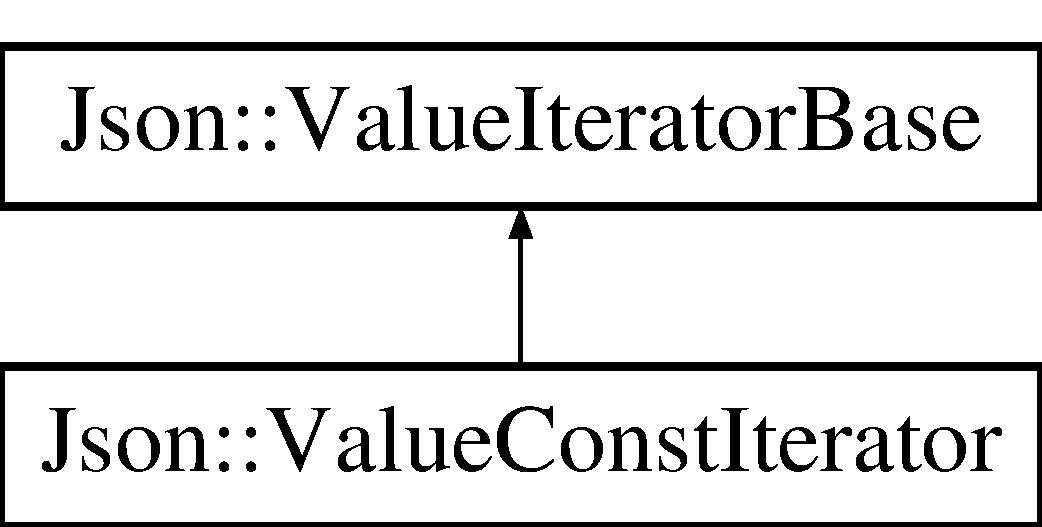
\includegraphics[height=2.000000cm]{classJson_1_1ValueConstIterator}
\end{center}
\end{figure}
\subsection*{Public Types}
\begin{DoxyCompactItemize}
\item 
typedef const \hyperlink{classJson_1_1Value}{Value} \hyperlink{classJson_1_1ValueConstIterator_aa5f1707dcef4bfe73e23ddc14dbe760d}{value\+\_\+type}
\item 
typedef const \hyperlink{classJson_1_1Value}{Value} \& \hyperlink{classJson_1_1ValueConstIterator_aa9b05c6a37cd352ea1ee6e13b816f709}{reference}
\item 
typedef const \hyperlink{classJson_1_1Value}{Value} $\ast$ \hyperlink{classJson_1_1ValueConstIterator_a400136bd8bc09e9fddec0785fa2cff14}{pointer}
\item 
typedef \hyperlink{classJson_1_1ValueConstIterator}{Value\+Const\+Iterator} \hyperlink{classJson_1_1ValueConstIterator_a0c2e33e7eb5a80dd8709fb28ece83933}{Self\+Type}
\item 
typedef std\+::bidirectional\+\_\+iterator\+\_\+tag \hyperlink{classJson_1_1ValueIteratorBase_a02fd11a4fbdc0007da1e8bcf5e6b83c3}{iterator\+\_\+category}
\item 
typedef unsigned int \hyperlink{classJson_1_1ValueIteratorBase_a9d3a3c7ce5cdefe23cb486239cf07bb5}{size\+\_\+t}
\item 
typedef int \hyperlink{classJson_1_1ValueIteratorBase_a4e44bf8cbd17ec8d6e2c185904a15ebd}{difference\+\_\+type}
\end{DoxyCompactItemize}
\subsection*{Public Member Functions}
\begin{DoxyCompactItemize}
\item 
\hyperlink{classJson_1_1ValueConstIterator_a1b10a46f1606421b0663492a5f9a2aad}{Value\+Const\+Iterator} ()
\item 
\hyperlink{classJson_1_1ValueConstIterator_a7ef3df204a9ae83a0d8a3cd128e05c70}{Value\+Const\+Iterator} (\hyperlink{classJson_1_1ValueIterator}{Value\+Iterator} const \&other)
\item 
\hyperlink{classJson_1_1ValueIteratorBase_a9d2a940d03ea06d20d972f41a89149ee}{Self\+Type} \& \hyperlink{classJson_1_1ValueConstIterator_ad1b1c11f8d7fb22d4d3c231915f2b15b}{operator=} (const \hyperlink{classJson_1_1ValueIteratorBase}{Value\+Iterator\+Base} \&other)
\item 
\hyperlink{classJson_1_1ValueIteratorBase_a9d2a940d03ea06d20d972f41a89149ee}{Self\+Type} \hyperlink{classJson_1_1ValueConstIterator_ab3f0c2edbfc8f7d60645f3d597d05e28}{operator++} (int)
\item 
\hyperlink{classJson_1_1ValueIteratorBase_a9d2a940d03ea06d20d972f41a89149ee}{Self\+Type} \hyperlink{classJson_1_1ValueConstIterator_a94935961e9331c6f7b907b05ec8df75e}{operator-\/-\/} (int)
\item 
\hyperlink{classJson_1_1ValueIteratorBase_a9d2a940d03ea06d20d972f41a89149ee}{Self\+Type} \& \hyperlink{classJson_1_1ValueConstIterator_a31415e44e44e56fb2bfda7e8bb784646}{operator-\/-\/} ()
\item 
\hyperlink{classJson_1_1ValueIteratorBase_a9d2a940d03ea06d20d972f41a89149ee}{Self\+Type} \& \hyperlink{classJson_1_1ValueConstIterator_a2cfe2f7a94a688186efdafb1b181c319}{operator++} ()
\item 
\hyperlink{classJson_1_1ValueConstIterator_aa9b05c6a37cd352ea1ee6e13b816f709}{reference} \hyperlink{classJson_1_1ValueConstIterator_aeb44153d71c61ac9397a84d5ecc244c5}{operator$\ast$} () const 
\item 
\hyperlink{classJson_1_1ValueConstIterator_a400136bd8bc09e9fddec0785fa2cff14}{pointer} \hyperlink{classJson_1_1ValueConstIterator_ac493d31c8eede8af10b71415fe8e624b}{operator-\/$>$} () const 
\item 
bool \hyperlink{classJson_1_1ValueIteratorBase_afc656672ac28502f640ade32c38c1b56}{operator==} (const \hyperlink{classJson_1_1ValueIteratorBase_a9d2a940d03ea06d20d972f41a89149ee}{Self\+Type} \&other) const 
\item 
bool \hyperlink{classJson_1_1ValueIteratorBase_a18c2dd42e0bb989ace141bfe9de52792}{operator!=} (const \hyperlink{classJson_1_1ValueIteratorBase_a9d2a940d03ea06d20d972f41a89149ee}{Self\+Type} \&other) const 
\item 
\hyperlink{classJson_1_1ValueIteratorBase_a4e44bf8cbd17ec8d6e2c185904a15ebd}{difference\+\_\+type} \hyperlink{classJson_1_1ValueIteratorBase_ab786787fcad68ca5e8745aaf520fa17f}{operator-\/} (const \hyperlink{classJson_1_1ValueIteratorBase_a9d2a940d03ea06d20d972f41a89149ee}{Self\+Type} \&other) const 
\item 
\hyperlink{classJson_1_1Value}{Value} \hyperlink{classJson_1_1ValueIteratorBase_aa2ff5e79fc96acd4c3cd288e92614fc7}{key} () const 
\begin{DoxyCompactList}\small\item\em Return either the index or the member name of the referenced value as a \hyperlink{classJson_1_1Value}{Value}. \end{DoxyCompactList}\item 
\hyperlink{namespaceJson_a800fb90eb6ee8d5d62b600c06f87f7d4}{U\+Int} \hyperlink{classJson_1_1ValueIteratorBase_aa90591f5f7f8d2f06cc4605816b53738}{index} () const 
\begin{DoxyCompactList}\small\item\em Return the index of the referenced \hyperlink{classJson_1_1Value}{Value}, or -\/1 if it is not an array\+Value. \end{DoxyCompactList}\item 
\hyperlink{json_8hpp_a1e723f95759de062585bc4a8fd3fa4be}{J\+S\+O\+N\+C\+P\+P\+\_\+\+S\+T\+R\+I\+NG} \hyperlink{classJson_1_1ValueIteratorBase_a99026427eb156ce007ef94df002e233f}{name} () const 
\begin{DoxyCompactList}\small\item\em Return the member name of the referenced \hyperlink{classJson_1_1Value}{Value}, or \char`\"{}\char`\"{} if it is not an object\+Value. \end{DoxyCompactList}\item 
char const $\ast$ \hyperlink{classJson_1_1ValueIteratorBase_ac3aa3870761342e47c6486d81f643c6c}{member\+Name} () const 
\begin{DoxyCompactList}\small\item\em Return the member name of the referenced \hyperlink{classJson_1_1Value}{Value}. \end{DoxyCompactList}\item 
char const $\ast$ \hyperlink{classJson_1_1ValueIteratorBase_a543d4e73e3d2d121bc287b24231386c3}{member\+Name} (char const $\ast$$\ast$end) const 
\begin{DoxyCompactList}\small\item\em Return the member name of the referenced \hyperlink{classJson_1_1Value}{Value}, or N\+U\+LL if it is not an object\+Value. \end{DoxyCompactList}\end{DoxyCompactItemize}
\subsection*{Protected Member Functions}
\begin{DoxyCompactItemize}
\item 
\hyperlink{classJson_1_1Value}{Value} \& \hyperlink{classJson_1_1ValueIteratorBase_a40a20c65abc423a26e3aae68d9a0525c}{deref} () const 
\item 
void \hyperlink{classJson_1_1ValueIteratorBase_afe58f9534e1fd2033419fd9fe244551e}{increment} ()
\item 
void \hyperlink{classJson_1_1ValueIteratorBase_affc8cf5ff54a9f432cc693362c153fa6}{decrement} ()
\item 
\hyperlink{classJson_1_1ValueIteratorBase_a4e44bf8cbd17ec8d6e2c185904a15ebd}{difference\+\_\+type} \hyperlink{classJson_1_1ValueIteratorBase_ad6c553b249e89e3dc9933e100ccbe064}{compute\+Distance} (const \hyperlink{classJson_1_1ValueIteratorBase_a9d2a940d03ea06d20d972f41a89149ee}{Self\+Type} \&other) const 
\item 
bool \hyperlink{classJson_1_1ValueIteratorBase_a21820d6ee564e541bd118b21e4741962}{is\+Equal} (const \hyperlink{classJson_1_1ValueIteratorBase_a9d2a940d03ea06d20d972f41a89149ee}{Self\+Type} \&other) const 
\item 
void \hyperlink{classJson_1_1ValueIteratorBase_a496e6aba44808433ec5858c178be5719}{copy} (const \hyperlink{classJson_1_1ValueIteratorBase_a9d2a940d03ea06d20d972f41a89149ee}{Self\+Type} \&other)
\end{DoxyCompactItemize}
\subsection*{Private Member Functions}
\begin{DoxyCompactItemize}
\item 
\hyperlink{classJson_1_1ValueConstIterator_aa0a87edf5f1097f91dca5f2a389c4abd}{Value\+Const\+Iterator} (const Value\+::\+Object\+Values\+::iterator \&current)
\end{DoxyCompactItemize}
\subsection*{Friends}
\begin{DoxyCompactItemize}
\item 
class \hyperlink{classJson_1_1ValueConstIterator_aeceedf6e1a7d48a588516ce2b1983d6f}{Value}
\end{DoxyCompactItemize}


\subsection{Detailed Description}
const iterator for object and array value. 

\subsection{Member Typedef Documentation}
\index{Json\+::\+Value\+Const\+Iterator@{Json\+::\+Value\+Const\+Iterator}!difference\+\_\+type@{difference\+\_\+type}}
\index{difference\+\_\+type@{difference\+\_\+type}!Json\+::\+Value\+Const\+Iterator@{Json\+::\+Value\+Const\+Iterator}}
\subsubsection[{\texorpdfstring{difference\+\_\+type}{difference_type}}]{\setlength{\rightskip}{0pt plus 5cm}typedef int {\bf Json\+::\+Value\+Iterator\+Base\+::difference\+\_\+type}\hspace{0.3cm}{\ttfamily [inherited]}}\hypertarget{classJson_1_1ValueIteratorBase_a4e44bf8cbd17ec8d6e2c185904a15ebd}{}\label{classJson_1_1ValueIteratorBase_a4e44bf8cbd17ec8d6e2c185904a15ebd}
\index{Json\+::\+Value\+Const\+Iterator@{Json\+::\+Value\+Const\+Iterator}!iterator\+\_\+category@{iterator\+\_\+category}}
\index{iterator\+\_\+category@{iterator\+\_\+category}!Json\+::\+Value\+Const\+Iterator@{Json\+::\+Value\+Const\+Iterator}}
\subsubsection[{\texorpdfstring{iterator\+\_\+category}{iterator_category}}]{\setlength{\rightskip}{0pt plus 5cm}typedef std\+::bidirectional\+\_\+iterator\+\_\+tag {\bf Json\+::\+Value\+Iterator\+Base\+::iterator\+\_\+category}\hspace{0.3cm}{\ttfamily [inherited]}}\hypertarget{classJson_1_1ValueIteratorBase_a02fd11a4fbdc0007da1e8bcf5e6b83c3}{}\label{classJson_1_1ValueIteratorBase_a02fd11a4fbdc0007da1e8bcf5e6b83c3}
\index{Json\+::\+Value\+Const\+Iterator@{Json\+::\+Value\+Const\+Iterator}!pointer@{pointer}}
\index{pointer@{pointer}!Json\+::\+Value\+Const\+Iterator@{Json\+::\+Value\+Const\+Iterator}}
\subsubsection[{\texorpdfstring{pointer}{pointer}}]{\setlength{\rightskip}{0pt plus 5cm}typedef const {\bf Value}$\ast$ {\bf Json\+::\+Value\+Const\+Iterator\+::pointer}}\hypertarget{classJson_1_1ValueConstIterator_a400136bd8bc09e9fddec0785fa2cff14}{}\label{classJson_1_1ValueConstIterator_a400136bd8bc09e9fddec0785fa2cff14}
\index{Json\+::\+Value\+Const\+Iterator@{Json\+::\+Value\+Const\+Iterator}!reference@{reference}}
\index{reference@{reference}!Json\+::\+Value\+Const\+Iterator@{Json\+::\+Value\+Const\+Iterator}}
\subsubsection[{\texorpdfstring{reference}{reference}}]{\setlength{\rightskip}{0pt plus 5cm}typedef const {\bf Value}\& {\bf Json\+::\+Value\+Const\+Iterator\+::reference}}\hypertarget{classJson_1_1ValueConstIterator_aa9b05c6a37cd352ea1ee6e13b816f709}{}\label{classJson_1_1ValueConstIterator_aa9b05c6a37cd352ea1ee6e13b816f709}
\index{Json\+::\+Value\+Const\+Iterator@{Json\+::\+Value\+Const\+Iterator}!Self\+Type@{Self\+Type}}
\index{Self\+Type@{Self\+Type}!Json\+::\+Value\+Const\+Iterator@{Json\+::\+Value\+Const\+Iterator}}
\subsubsection[{\texorpdfstring{Self\+Type}{SelfType}}]{\setlength{\rightskip}{0pt plus 5cm}typedef {\bf Value\+Const\+Iterator} {\bf Json\+::\+Value\+Const\+Iterator\+::\+Self\+Type}}\hypertarget{classJson_1_1ValueConstIterator_a0c2e33e7eb5a80dd8709fb28ece83933}{}\label{classJson_1_1ValueConstIterator_a0c2e33e7eb5a80dd8709fb28ece83933}
\index{Json\+::\+Value\+Const\+Iterator@{Json\+::\+Value\+Const\+Iterator}!size\+\_\+t@{size\+\_\+t}}
\index{size\+\_\+t@{size\+\_\+t}!Json\+::\+Value\+Const\+Iterator@{Json\+::\+Value\+Const\+Iterator}}
\subsubsection[{\texorpdfstring{size\+\_\+t}{size_t}}]{\setlength{\rightskip}{0pt plus 5cm}typedef unsigned int {\bf Json\+::\+Value\+Iterator\+Base\+::size\+\_\+t}\hspace{0.3cm}{\ttfamily [inherited]}}\hypertarget{classJson_1_1ValueIteratorBase_a9d3a3c7ce5cdefe23cb486239cf07bb5}{}\label{classJson_1_1ValueIteratorBase_a9d3a3c7ce5cdefe23cb486239cf07bb5}
\index{Json\+::\+Value\+Const\+Iterator@{Json\+::\+Value\+Const\+Iterator}!value\+\_\+type@{value\+\_\+type}}
\index{value\+\_\+type@{value\+\_\+type}!Json\+::\+Value\+Const\+Iterator@{Json\+::\+Value\+Const\+Iterator}}
\subsubsection[{\texorpdfstring{value\+\_\+type}{value_type}}]{\setlength{\rightskip}{0pt plus 5cm}typedef const {\bf Value} {\bf Json\+::\+Value\+Const\+Iterator\+::value\+\_\+type}}\hypertarget{classJson_1_1ValueConstIterator_aa5f1707dcef4bfe73e23ddc14dbe760d}{}\label{classJson_1_1ValueConstIterator_aa5f1707dcef4bfe73e23ddc14dbe760d}


\subsection{Constructor \& Destructor Documentation}
\index{Json\+::\+Value\+Const\+Iterator@{Json\+::\+Value\+Const\+Iterator}!Value\+Const\+Iterator@{Value\+Const\+Iterator}}
\index{Value\+Const\+Iterator@{Value\+Const\+Iterator}!Json\+::\+Value\+Const\+Iterator@{Json\+::\+Value\+Const\+Iterator}}
\subsubsection[{\texorpdfstring{Value\+Const\+Iterator()}{ValueConstIterator()}}]{\setlength{\rightskip}{0pt plus 5cm}Json\+::\+Value\+Const\+Iterator\+::\+Value\+Const\+Iterator (
\begin{DoxyParamCaption}
{}
\end{DoxyParamCaption}
)}\hypertarget{classJson_1_1ValueConstIterator_a1b10a46f1606421b0663492a5f9a2aad}{}\label{classJson_1_1ValueConstIterator_a1b10a46f1606421b0663492a5f9a2aad}
\index{Json\+::\+Value\+Const\+Iterator@{Json\+::\+Value\+Const\+Iterator}!Value\+Const\+Iterator@{Value\+Const\+Iterator}}
\index{Value\+Const\+Iterator@{Value\+Const\+Iterator}!Json\+::\+Value\+Const\+Iterator@{Json\+::\+Value\+Const\+Iterator}}
\subsubsection[{\texorpdfstring{Value\+Const\+Iterator(\+Value\+Iterator const \&other)}{ValueConstIterator(ValueIterator const &other)}}]{\setlength{\rightskip}{0pt plus 5cm}Json\+::\+Value\+Const\+Iterator\+::\+Value\+Const\+Iterator (
\begin{DoxyParamCaption}
\item[{{\bf Value\+Iterator} const \&}]{other}
\end{DoxyParamCaption}
)}\hypertarget{classJson_1_1ValueConstIterator_a7ef3df204a9ae83a0d8a3cd128e05c70}{}\label{classJson_1_1ValueConstIterator_a7ef3df204a9ae83a0d8a3cd128e05c70}
\index{Json\+::\+Value\+Const\+Iterator@{Json\+::\+Value\+Const\+Iterator}!Value\+Const\+Iterator@{Value\+Const\+Iterator}}
\index{Value\+Const\+Iterator@{Value\+Const\+Iterator}!Json\+::\+Value\+Const\+Iterator@{Json\+::\+Value\+Const\+Iterator}}
\subsubsection[{\texorpdfstring{Value\+Const\+Iterator(const Value\+::\+Object\+Values\+::iterator \&current)}{ValueConstIterator(const Value::ObjectValues::iterator &current)}}]{\setlength{\rightskip}{0pt plus 5cm}Json\+::\+Value\+Const\+Iterator\+::\+Value\+Const\+Iterator (
\begin{DoxyParamCaption}
\item[{const Value\+::\+Object\+Values\+::iterator \&}]{current}
\end{DoxyParamCaption}
)\hspace{0.3cm}{\ttfamily [explicit]}, {\ttfamily [private]}}\hypertarget{classJson_1_1ValueConstIterator_aa0a87edf5f1097f91dca5f2a389c4abd}{}\label{classJson_1_1ValueConstIterator_aa0a87edf5f1097f91dca5f2a389c4abd}


\subsection{Member Function Documentation}
\index{Json\+::\+Value\+Const\+Iterator@{Json\+::\+Value\+Const\+Iterator}!compute\+Distance@{compute\+Distance}}
\index{compute\+Distance@{compute\+Distance}!Json\+::\+Value\+Const\+Iterator@{Json\+::\+Value\+Const\+Iterator}}
\subsubsection[{\texorpdfstring{compute\+Distance(const Self\+Type \&other) const }{computeDistance(const SelfType &other) const }}]{\setlength{\rightskip}{0pt plus 5cm}{\bf Value\+Iterator\+Base\+::difference\+\_\+type} Json\+::\+Value\+Iterator\+Base\+::compute\+Distance (
\begin{DoxyParamCaption}
\item[{const {\bf Self\+Type} \&}]{other}
\end{DoxyParamCaption}
) const\hspace{0.3cm}{\ttfamily [protected]}, {\ttfamily [inherited]}}\hypertarget{classJson_1_1ValueIteratorBase_ad6c553b249e89e3dc9933e100ccbe064}{}\label{classJson_1_1ValueIteratorBase_ad6c553b249e89e3dc9933e100ccbe064}
\index{Json\+::\+Value\+Const\+Iterator@{Json\+::\+Value\+Const\+Iterator}!copy@{copy}}
\index{copy@{copy}!Json\+::\+Value\+Const\+Iterator@{Json\+::\+Value\+Const\+Iterator}}
\subsubsection[{\texorpdfstring{copy(const Self\+Type \&other)}{copy(const SelfType &other)}}]{\setlength{\rightskip}{0pt plus 5cm}void Json\+::\+Value\+Iterator\+Base\+::copy (
\begin{DoxyParamCaption}
\item[{const {\bf Self\+Type} \&}]{other}
\end{DoxyParamCaption}
)\hspace{0.3cm}{\ttfamily [protected]}, {\ttfamily [inherited]}}\hypertarget{classJson_1_1ValueIteratorBase_a496e6aba44808433ec5858c178be5719}{}\label{classJson_1_1ValueIteratorBase_a496e6aba44808433ec5858c178be5719}
\index{Json\+::\+Value\+Const\+Iterator@{Json\+::\+Value\+Const\+Iterator}!decrement@{decrement}}
\index{decrement@{decrement}!Json\+::\+Value\+Const\+Iterator@{Json\+::\+Value\+Const\+Iterator}}
\subsubsection[{\texorpdfstring{decrement()}{decrement()}}]{\setlength{\rightskip}{0pt plus 5cm}void Json\+::\+Value\+Iterator\+Base\+::decrement (
\begin{DoxyParamCaption}
{}
\end{DoxyParamCaption}
)\hspace{0.3cm}{\ttfamily [protected]}, {\ttfamily [inherited]}}\hypertarget{classJson_1_1ValueIteratorBase_affc8cf5ff54a9f432cc693362c153fa6}{}\label{classJson_1_1ValueIteratorBase_affc8cf5ff54a9f432cc693362c153fa6}
\index{Json\+::\+Value\+Const\+Iterator@{Json\+::\+Value\+Const\+Iterator}!deref@{deref}}
\index{deref@{deref}!Json\+::\+Value\+Const\+Iterator@{Json\+::\+Value\+Const\+Iterator}}
\subsubsection[{\texorpdfstring{deref() const }{deref() const }}]{\setlength{\rightskip}{0pt plus 5cm}{\bf Value} \& Json\+::\+Value\+Iterator\+Base\+::deref (
\begin{DoxyParamCaption}
{}
\end{DoxyParamCaption}
) const\hspace{0.3cm}{\ttfamily [protected]}, {\ttfamily [inherited]}}\hypertarget{classJson_1_1ValueIteratorBase_a40a20c65abc423a26e3aae68d9a0525c}{}\label{classJson_1_1ValueIteratorBase_a40a20c65abc423a26e3aae68d9a0525c}
\index{Json\+::\+Value\+Const\+Iterator@{Json\+::\+Value\+Const\+Iterator}!increment@{increment}}
\index{increment@{increment}!Json\+::\+Value\+Const\+Iterator@{Json\+::\+Value\+Const\+Iterator}}
\subsubsection[{\texorpdfstring{increment()}{increment()}}]{\setlength{\rightskip}{0pt plus 5cm}void Json\+::\+Value\+Iterator\+Base\+::increment (
\begin{DoxyParamCaption}
{}
\end{DoxyParamCaption}
)\hspace{0.3cm}{\ttfamily [protected]}, {\ttfamily [inherited]}}\hypertarget{classJson_1_1ValueIteratorBase_afe58f9534e1fd2033419fd9fe244551e}{}\label{classJson_1_1ValueIteratorBase_afe58f9534e1fd2033419fd9fe244551e}
\index{Json\+::\+Value\+Const\+Iterator@{Json\+::\+Value\+Const\+Iterator}!index@{index}}
\index{index@{index}!Json\+::\+Value\+Const\+Iterator@{Json\+::\+Value\+Const\+Iterator}}
\subsubsection[{\texorpdfstring{index() const }{index() const }}]{\setlength{\rightskip}{0pt plus 5cm}{\bf U\+Int} Json\+::\+Value\+Iterator\+Base\+::index (
\begin{DoxyParamCaption}
{}
\end{DoxyParamCaption}
) const\hspace{0.3cm}{\ttfamily [inherited]}}\hypertarget{classJson_1_1ValueIteratorBase_aa90591f5f7f8d2f06cc4605816b53738}{}\label{classJson_1_1ValueIteratorBase_aa90591f5f7f8d2f06cc4605816b53738}


Return the index of the referenced \hyperlink{classJson_1_1Value}{Value}, or -\/1 if it is not an array\+Value. 

\index{Json\+::\+Value\+Const\+Iterator@{Json\+::\+Value\+Const\+Iterator}!is\+Equal@{is\+Equal}}
\index{is\+Equal@{is\+Equal}!Json\+::\+Value\+Const\+Iterator@{Json\+::\+Value\+Const\+Iterator}}
\subsubsection[{\texorpdfstring{is\+Equal(const Self\+Type \&other) const }{isEqual(const SelfType &other) const }}]{\setlength{\rightskip}{0pt plus 5cm}bool Json\+::\+Value\+Iterator\+Base\+::is\+Equal (
\begin{DoxyParamCaption}
\item[{const {\bf Self\+Type} \&}]{other}
\end{DoxyParamCaption}
) const\hspace{0.3cm}{\ttfamily [protected]}, {\ttfamily [inherited]}}\hypertarget{classJson_1_1ValueIteratorBase_a21820d6ee564e541bd118b21e4741962}{}\label{classJson_1_1ValueIteratorBase_a21820d6ee564e541bd118b21e4741962}
\index{Json\+::\+Value\+Const\+Iterator@{Json\+::\+Value\+Const\+Iterator}!key@{key}}
\index{key@{key}!Json\+::\+Value\+Const\+Iterator@{Json\+::\+Value\+Const\+Iterator}}
\subsubsection[{\texorpdfstring{key() const }{key() const }}]{\setlength{\rightskip}{0pt plus 5cm}{\bf Value} Json\+::\+Value\+Iterator\+Base\+::key (
\begin{DoxyParamCaption}
{}
\end{DoxyParamCaption}
) const\hspace{0.3cm}{\ttfamily [inherited]}}\hypertarget{classJson_1_1ValueIteratorBase_aa2ff5e79fc96acd4c3cd288e92614fc7}{}\label{classJson_1_1ValueIteratorBase_aa2ff5e79fc96acd4c3cd288e92614fc7}


Return either the index or the member name of the referenced value as a \hyperlink{classJson_1_1Value}{Value}. 

\index{Json\+::\+Value\+Const\+Iterator@{Json\+::\+Value\+Const\+Iterator}!member\+Name@{member\+Name}}
\index{member\+Name@{member\+Name}!Json\+::\+Value\+Const\+Iterator@{Json\+::\+Value\+Const\+Iterator}}
\subsubsection[{\texorpdfstring{member\+Name() const }{memberName() const }}]{\setlength{\rightskip}{0pt plus 5cm}char const $\ast$ Json\+::\+Value\+Iterator\+Base\+::member\+Name (
\begin{DoxyParamCaption}
{}
\end{DoxyParamCaption}
) const\hspace{0.3cm}{\ttfamily [inherited]}}\hypertarget{classJson_1_1ValueIteratorBase_ac3aa3870761342e47c6486d81f643c6c}{}\label{classJson_1_1ValueIteratorBase_ac3aa3870761342e47c6486d81f643c6c}


Return the member name of the referenced \hyperlink{classJson_1_1Value}{Value}. 

\char`\"{}\char`\"{} if it is not an object\+Value. \begin{DoxyRefDesc}{Deprecated}
\item[\hyperlink{deprecated__deprecated000004}{Deprecated}]This cannot be used for U\+T\+F-\/8 strings, since there can be embedded nulls. \end{DoxyRefDesc}
\index{Json\+::\+Value\+Const\+Iterator@{Json\+::\+Value\+Const\+Iterator}!member\+Name@{member\+Name}}
\index{member\+Name@{member\+Name}!Json\+::\+Value\+Const\+Iterator@{Json\+::\+Value\+Const\+Iterator}}
\subsubsection[{\texorpdfstring{member\+Name(char const $\ast$$\ast$end) const }{memberName(char const **end) const }}]{\setlength{\rightskip}{0pt plus 5cm}char const $\ast$ Json\+::\+Value\+Iterator\+Base\+::member\+Name (
\begin{DoxyParamCaption}
\item[{char const $\ast$$\ast$}]{end}
\end{DoxyParamCaption}
) const\hspace{0.3cm}{\ttfamily [inherited]}}\hypertarget{classJson_1_1ValueIteratorBase_a543d4e73e3d2d121bc287b24231386c3}{}\label{classJson_1_1ValueIteratorBase_a543d4e73e3d2d121bc287b24231386c3}


Return the member name of the referenced \hyperlink{classJson_1_1Value}{Value}, or N\+U\+LL if it is not an object\+Value. 

\begin{DoxyNote}{Note}
Better version than \hyperlink{classJson_1_1ValueIteratorBase_ac3aa3870761342e47c6486d81f643c6c}{member\+Name()}. Allows embedded nulls. 
\end{DoxyNote}
\index{Json\+::\+Value\+Const\+Iterator@{Json\+::\+Value\+Const\+Iterator}!name@{name}}
\index{name@{name}!Json\+::\+Value\+Const\+Iterator@{Json\+::\+Value\+Const\+Iterator}}
\subsubsection[{\texorpdfstring{name() const }{name() const }}]{\setlength{\rightskip}{0pt plus 5cm}{\bf J\+S\+O\+N\+C\+P\+P\+\_\+\+S\+T\+R\+I\+NG} Json\+::\+Value\+Iterator\+Base\+::name (
\begin{DoxyParamCaption}
{}
\end{DoxyParamCaption}
) const\hspace{0.3cm}{\ttfamily [inherited]}}\hypertarget{classJson_1_1ValueIteratorBase_a99026427eb156ce007ef94df002e233f}{}\label{classJson_1_1ValueIteratorBase_a99026427eb156ce007ef94df002e233f}


Return the member name of the referenced \hyperlink{classJson_1_1Value}{Value}, or \char`\"{}\char`\"{} if it is not an object\+Value. 

\begin{DoxyNote}{Note}
Avoid {\ttfamily c\+\_\+str()} on result, as embedded zeroes are possible. 
\end{DoxyNote}
\index{Json\+::\+Value\+Const\+Iterator@{Json\+::\+Value\+Const\+Iterator}!operator"!=@{operator"!=}}
\index{operator"!=@{operator"!=}!Json\+::\+Value\+Const\+Iterator@{Json\+::\+Value\+Const\+Iterator}}
\subsubsection[{\texorpdfstring{operator"!=(const Self\+Type \&other) const }{operator!=(const SelfType &other) const }}]{\setlength{\rightskip}{0pt plus 5cm}bool Json\+::\+Value\+Iterator\+Base\+::operator!= (
\begin{DoxyParamCaption}
\item[{const {\bf Self\+Type} \&}]{other}
\end{DoxyParamCaption}
) const\hspace{0.3cm}{\ttfamily [inline]}, {\ttfamily [inherited]}}\hypertarget{classJson_1_1ValueIteratorBase_a18c2dd42e0bb989ace141bfe9de52792}{}\label{classJson_1_1ValueIteratorBase_a18c2dd42e0bb989ace141bfe9de52792}
\index{Json\+::\+Value\+Const\+Iterator@{Json\+::\+Value\+Const\+Iterator}!operator$\ast$@{operator$\ast$}}
\index{operator$\ast$@{operator$\ast$}!Json\+::\+Value\+Const\+Iterator@{Json\+::\+Value\+Const\+Iterator}}
\subsubsection[{\texorpdfstring{operator$\ast$() const }{operator*() const }}]{\setlength{\rightskip}{0pt plus 5cm}{\bf reference} Json\+::\+Value\+Const\+Iterator\+::operator$\ast$ (
\begin{DoxyParamCaption}
{}
\end{DoxyParamCaption}
) const\hspace{0.3cm}{\ttfamily [inline]}}\hypertarget{classJson_1_1ValueConstIterator_aeb44153d71c61ac9397a84d5ecc244c5}{}\label{classJson_1_1ValueConstIterator_aeb44153d71c61ac9397a84d5ecc244c5}
\index{Json\+::\+Value\+Const\+Iterator@{Json\+::\+Value\+Const\+Iterator}!operator++@{operator++}}
\index{operator++@{operator++}!Json\+::\+Value\+Const\+Iterator@{Json\+::\+Value\+Const\+Iterator}}
\subsubsection[{\texorpdfstring{operator++(int)}{operator++(int)}}]{\setlength{\rightskip}{0pt plus 5cm}{\bf Self\+Type} Json\+::\+Value\+Const\+Iterator\+::operator++ (
\begin{DoxyParamCaption}
\item[{int}]{}
\end{DoxyParamCaption}
)\hspace{0.3cm}{\ttfamily [inline]}}\hypertarget{classJson_1_1ValueConstIterator_ab3f0c2edbfc8f7d60645f3d597d05e28}{}\label{classJson_1_1ValueConstIterator_ab3f0c2edbfc8f7d60645f3d597d05e28}
\index{Json\+::\+Value\+Const\+Iterator@{Json\+::\+Value\+Const\+Iterator}!operator++@{operator++}}
\index{operator++@{operator++}!Json\+::\+Value\+Const\+Iterator@{Json\+::\+Value\+Const\+Iterator}}
\subsubsection[{\texorpdfstring{operator++()}{operator++()}}]{\setlength{\rightskip}{0pt plus 5cm}{\bf Self\+Type}\& Json\+::\+Value\+Const\+Iterator\+::operator++ (
\begin{DoxyParamCaption}
{}
\end{DoxyParamCaption}
)\hspace{0.3cm}{\ttfamily [inline]}}\hypertarget{classJson_1_1ValueConstIterator_a2cfe2f7a94a688186efdafb1b181c319}{}\label{classJson_1_1ValueConstIterator_a2cfe2f7a94a688186efdafb1b181c319}
\index{Json\+::\+Value\+Const\+Iterator@{Json\+::\+Value\+Const\+Iterator}!operator-\/@{operator-\/}}
\index{operator-\/@{operator-\/}!Json\+::\+Value\+Const\+Iterator@{Json\+::\+Value\+Const\+Iterator}}
\subsubsection[{\texorpdfstring{operator-\/(const Self\+Type \&other) const }{operator-(const SelfType &other) const }}]{\setlength{\rightskip}{0pt plus 5cm}{\bf difference\+\_\+type} Json\+::\+Value\+Iterator\+Base\+::operator-\/ (
\begin{DoxyParamCaption}
\item[{const {\bf Self\+Type} \&}]{other}
\end{DoxyParamCaption}
) const\hspace{0.3cm}{\ttfamily [inline]}, {\ttfamily [inherited]}}\hypertarget{classJson_1_1ValueIteratorBase_ab786787fcad68ca5e8745aaf520fa17f}{}\label{classJson_1_1ValueIteratorBase_ab786787fcad68ca5e8745aaf520fa17f}
\index{Json\+::\+Value\+Const\+Iterator@{Json\+::\+Value\+Const\+Iterator}!operator-\/-\/@{operator-\/-\/}}
\index{operator-\/-\/@{operator-\/-\/}!Json\+::\+Value\+Const\+Iterator@{Json\+::\+Value\+Const\+Iterator}}
\subsubsection[{\texorpdfstring{operator-\/-\/(int)}{operator--(int)}}]{\setlength{\rightskip}{0pt plus 5cm}{\bf Self\+Type} Json\+::\+Value\+Const\+Iterator\+::operator-\/-\/ (
\begin{DoxyParamCaption}
\item[{int}]{}
\end{DoxyParamCaption}
)\hspace{0.3cm}{\ttfamily [inline]}}\hypertarget{classJson_1_1ValueConstIterator_a94935961e9331c6f7b907b05ec8df75e}{}\label{classJson_1_1ValueConstIterator_a94935961e9331c6f7b907b05ec8df75e}
\index{Json\+::\+Value\+Const\+Iterator@{Json\+::\+Value\+Const\+Iterator}!operator-\/-\/@{operator-\/-\/}}
\index{operator-\/-\/@{operator-\/-\/}!Json\+::\+Value\+Const\+Iterator@{Json\+::\+Value\+Const\+Iterator}}
\subsubsection[{\texorpdfstring{operator-\/-\/()}{operator--()}}]{\setlength{\rightskip}{0pt plus 5cm}{\bf Self\+Type}\& Json\+::\+Value\+Const\+Iterator\+::operator-\/-\/ (
\begin{DoxyParamCaption}
{}
\end{DoxyParamCaption}
)\hspace{0.3cm}{\ttfamily [inline]}}\hypertarget{classJson_1_1ValueConstIterator_a31415e44e44e56fb2bfda7e8bb784646}{}\label{classJson_1_1ValueConstIterator_a31415e44e44e56fb2bfda7e8bb784646}
\index{Json\+::\+Value\+Const\+Iterator@{Json\+::\+Value\+Const\+Iterator}!operator-\/$>$@{operator-\/$>$}}
\index{operator-\/$>$@{operator-\/$>$}!Json\+::\+Value\+Const\+Iterator@{Json\+::\+Value\+Const\+Iterator}}
\subsubsection[{\texorpdfstring{operator-\/$>$() const }{operator->() const }}]{\setlength{\rightskip}{0pt plus 5cm}{\bf pointer} Json\+::\+Value\+Const\+Iterator\+::operator-\/$>$ (
\begin{DoxyParamCaption}
{}
\end{DoxyParamCaption}
) const\hspace{0.3cm}{\ttfamily [inline]}}\hypertarget{classJson_1_1ValueConstIterator_ac493d31c8eede8af10b71415fe8e624b}{}\label{classJson_1_1ValueConstIterator_ac493d31c8eede8af10b71415fe8e624b}
\index{Json\+::\+Value\+Const\+Iterator@{Json\+::\+Value\+Const\+Iterator}!operator=@{operator=}}
\index{operator=@{operator=}!Json\+::\+Value\+Const\+Iterator@{Json\+::\+Value\+Const\+Iterator}}
\subsubsection[{\texorpdfstring{operator=(const Value\+Iterator\+Base \&other)}{operator=(const ValueIteratorBase &other)}}]{\setlength{\rightskip}{0pt plus 5cm}{\bf Value\+Const\+Iterator} \& Json\+::\+Value\+Const\+Iterator\+::operator= (
\begin{DoxyParamCaption}
\item[{const {\bf Value\+Iterator\+Base} \&}]{other}
\end{DoxyParamCaption}
)}\hypertarget{classJson_1_1ValueConstIterator_ad1b1c11f8d7fb22d4d3c231915f2b15b}{}\label{classJson_1_1ValueConstIterator_ad1b1c11f8d7fb22d4d3c231915f2b15b}
\index{Json\+::\+Value\+Const\+Iterator@{Json\+::\+Value\+Const\+Iterator}!operator==@{operator==}}
\index{operator==@{operator==}!Json\+::\+Value\+Const\+Iterator@{Json\+::\+Value\+Const\+Iterator}}
\subsubsection[{\texorpdfstring{operator==(const Self\+Type \&other) const }{operator==(const SelfType &other) const }}]{\setlength{\rightskip}{0pt plus 5cm}bool Json\+::\+Value\+Iterator\+Base\+::operator== (
\begin{DoxyParamCaption}
\item[{const {\bf Self\+Type} \&}]{other}
\end{DoxyParamCaption}
) const\hspace{0.3cm}{\ttfamily [inline]}, {\ttfamily [inherited]}}\hypertarget{classJson_1_1ValueIteratorBase_afc656672ac28502f640ade32c38c1b56}{}\label{classJson_1_1ValueIteratorBase_afc656672ac28502f640ade32c38c1b56}


\subsection{Friends And Related Function Documentation}
\index{Json\+::\+Value\+Const\+Iterator@{Json\+::\+Value\+Const\+Iterator}!Value@{Value}}
\index{Value@{Value}!Json\+::\+Value\+Const\+Iterator@{Json\+::\+Value\+Const\+Iterator}}
\subsubsection[{\texorpdfstring{Value}{Value}}]{\setlength{\rightskip}{0pt plus 5cm}friend class {\bf Value}\hspace{0.3cm}{\ttfamily [friend]}}\hypertarget{classJson_1_1ValueConstIterator_aeceedf6e1a7d48a588516ce2b1983d6f}{}\label{classJson_1_1ValueConstIterator_aeceedf6e1a7d48a588516ce2b1983d6f}


The documentation for this class was generated from the following files\+:\begin{DoxyCompactItemize}
\item 
/home/pranav/\+Repositories/zcm/include/\hyperlink{json_8hpp}{json.\+hpp}\item 
/home/pranav/\+Repositories/zcm/src/\hyperlink{json_8cpp}{json.\+cpp}\end{DoxyCompactItemize}

\hypertarget{unionJson_1_1Value_1_1ValueHolder}{}\section{Json\+:\+:Value\+:\+:Value\+Holder Union Reference}
\label{unionJson_1_1Value_1_1ValueHolder}\index{Json\+::\+Value\+::\+Value\+Holder@{Json\+::\+Value\+::\+Value\+Holder}}
\subsection*{Public Attributes}
\begin{DoxyCompactItemize}
\item 
\hyperlink{classJson_1_1Value_a1cbb82642ed05109b9833e49f042ece7}{Largest\+Int} \hyperlink{unionJson_1_1Value_1_1ValueHolder_adbfb384301298844ed955ba5cf6015a0}{int\+\_\+}
\item 
\hyperlink{classJson_1_1Value_a6682a3684d635e03fc06ba229fa24eec}{Largest\+U\+Int} \hyperlink{unionJson_1_1Value_1_1ValueHolder_aab65665dc15a24a29a8e93cdeeaa7e50}{uint\+\_\+}
\item 
double \hyperlink{unionJson_1_1Value_1_1ValueHolder_af0c5ca724e5fe3a15db773d750e2351e}{real\+\_\+}
\item 
bool \hyperlink{unionJson_1_1Value_1_1ValueHolder_a92edab1861dadbfefd8be5fd4285eefe}{bool\+\_\+}
\item 
char $\ast$ \hyperlink{unionJson_1_1Value_1_1ValueHolder_a70ac2b153bc405527baa3850d2ddc3cb}{string\+\_\+}
\item 
\hyperlink{classJson_1_1Value_a08b6c80c3af7071d908dabf044de5388}{Object\+Values} $\ast$ \hyperlink{unionJson_1_1Value_1_1ValueHolder_a1e7a5b86d4f52234f55c847ad1ce389a}{map\+\_\+}
\end{DoxyCompactItemize}


\subsection{Member Data Documentation}
\index{Json\+::\+Value\+::\+Value\+Holder@{Json\+::\+Value\+::\+Value\+Holder}!bool\+\_\+@{bool\+\_\+}}
\index{bool\+\_\+@{bool\+\_\+}!Json\+::\+Value\+::\+Value\+Holder@{Json\+::\+Value\+::\+Value\+Holder}}
\subsubsection[{\texorpdfstring{bool\+\_\+}{bool_}}]{\setlength{\rightskip}{0pt plus 5cm}bool Json\+::\+Value\+::\+Value\+Holder\+::bool\+\_\+}\hypertarget{unionJson_1_1Value_1_1ValueHolder_a92edab1861dadbfefd8be5fd4285eefe}{}\label{unionJson_1_1Value_1_1ValueHolder_a92edab1861dadbfefd8be5fd4285eefe}
\index{Json\+::\+Value\+::\+Value\+Holder@{Json\+::\+Value\+::\+Value\+Holder}!int\+\_\+@{int\+\_\+}}
\index{int\+\_\+@{int\+\_\+}!Json\+::\+Value\+::\+Value\+Holder@{Json\+::\+Value\+::\+Value\+Holder}}
\subsubsection[{\texorpdfstring{int\+\_\+}{int_}}]{\setlength{\rightskip}{0pt plus 5cm}{\bf Largest\+Int} Json\+::\+Value\+::\+Value\+Holder\+::int\+\_\+}\hypertarget{unionJson_1_1Value_1_1ValueHolder_adbfb384301298844ed955ba5cf6015a0}{}\label{unionJson_1_1Value_1_1ValueHolder_adbfb384301298844ed955ba5cf6015a0}
\index{Json\+::\+Value\+::\+Value\+Holder@{Json\+::\+Value\+::\+Value\+Holder}!map\+\_\+@{map\+\_\+}}
\index{map\+\_\+@{map\+\_\+}!Json\+::\+Value\+::\+Value\+Holder@{Json\+::\+Value\+::\+Value\+Holder}}
\subsubsection[{\texorpdfstring{map\+\_\+}{map_}}]{\setlength{\rightskip}{0pt plus 5cm}{\bf Object\+Values}$\ast$ Json\+::\+Value\+::\+Value\+Holder\+::map\+\_\+}\hypertarget{unionJson_1_1Value_1_1ValueHolder_a1e7a5b86d4f52234f55c847ad1ce389a}{}\label{unionJson_1_1Value_1_1ValueHolder_a1e7a5b86d4f52234f55c847ad1ce389a}
\index{Json\+::\+Value\+::\+Value\+Holder@{Json\+::\+Value\+::\+Value\+Holder}!real\+\_\+@{real\+\_\+}}
\index{real\+\_\+@{real\+\_\+}!Json\+::\+Value\+::\+Value\+Holder@{Json\+::\+Value\+::\+Value\+Holder}}
\subsubsection[{\texorpdfstring{real\+\_\+}{real_}}]{\setlength{\rightskip}{0pt plus 5cm}double Json\+::\+Value\+::\+Value\+Holder\+::real\+\_\+}\hypertarget{unionJson_1_1Value_1_1ValueHolder_af0c5ca724e5fe3a15db773d750e2351e}{}\label{unionJson_1_1Value_1_1ValueHolder_af0c5ca724e5fe3a15db773d750e2351e}
\index{Json\+::\+Value\+::\+Value\+Holder@{Json\+::\+Value\+::\+Value\+Holder}!string\+\_\+@{string\+\_\+}}
\index{string\+\_\+@{string\+\_\+}!Json\+::\+Value\+::\+Value\+Holder@{Json\+::\+Value\+::\+Value\+Holder}}
\subsubsection[{\texorpdfstring{string\+\_\+}{string_}}]{\setlength{\rightskip}{0pt plus 5cm}char$\ast$ Json\+::\+Value\+::\+Value\+Holder\+::string\+\_\+}\hypertarget{unionJson_1_1Value_1_1ValueHolder_a70ac2b153bc405527baa3850d2ddc3cb}{}\label{unionJson_1_1Value_1_1ValueHolder_a70ac2b153bc405527baa3850d2ddc3cb}
\index{Json\+::\+Value\+::\+Value\+Holder@{Json\+::\+Value\+::\+Value\+Holder}!uint\+\_\+@{uint\+\_\+}}
\index{uint\+\_\+@{uint\+\_\+}!Json\+::\+Value\+::\+Value\+Holder@{Json\+::\+Value\+::\+Value\+Holder}}
\subsubsection[{\texorpdfstring{uint\+\_\+}{uint_}}]{\setlength{\rightskip}{0pt plus 5cm}{\bf Largest\+U\+Int} Json\+::\+Value\+::\+Value\+Holder\+::uint\+\_\+}\hypertarget{unionJson_1_1Value_1_1ValueHolder_aab65665dc15a24a29a8e93cdeeaa7e50}{}\label{unionJson_1_1Value_1_1ValueHolder_aab65665dc15a24a29a8e93cdeeaa7e50}


The documentation for this union was generated from the following file\+:\begin{DoxyCompactItemize}
\item 
/home/pranav/\+Repositories/zcm/include/\hyperlink{json_8hpp}{json.\+hpp}\end{DoxyCompactItemize}

\hypertarget{classJson_1_1ValueIterator}{}\section{Json\+:\+:Value\+Iterator Class Reference}
\label{classJson_1_1ValueIterator}\index{Json\+::\+Value\+Iterator@{Json\+::\+Value\+Iterator}}


Iterator for object and array value.  




{\ttfamily \#include $<$json.\+hpp$>$}

Inheritance diagram for Json\+:\+:Value\+Iterator\+:\begin{figure}[H]
\begin{center}
\leavevmode
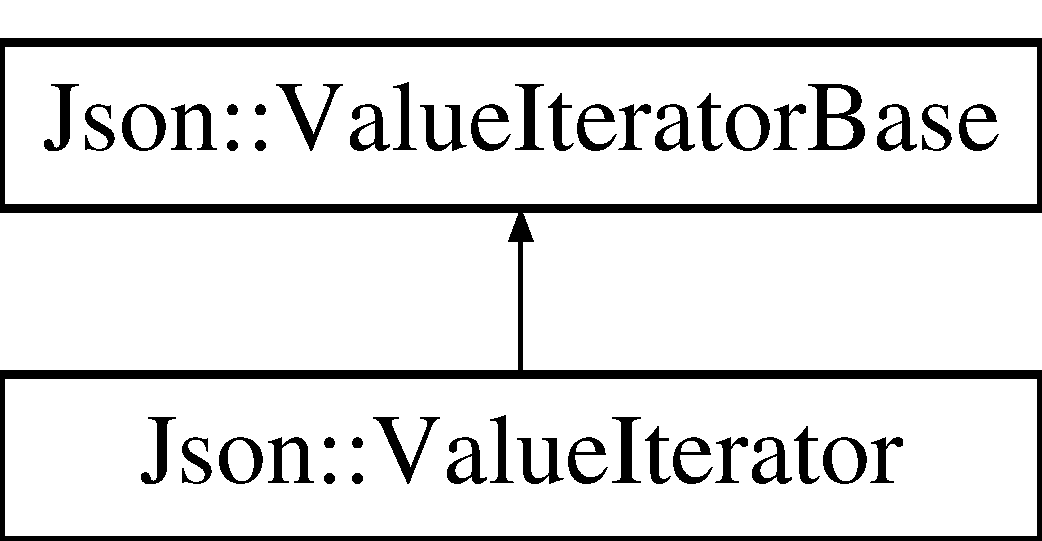
\includegraphics[height=2.000000cm]{classJson_1_1ValueIterator}
\end{center}
\end{figure}
\subsection*{Public Types}
\begin{DoxyCompactItemize}
\item 
typedef \hyperlink{classJson_1_1Value}{Value} \hyperlink{classJson_1_1ValueIterator_a2c5ba7be611f05546530c8a88b2d2e37}{value\+\_\+type}
\item 
typedef unsigned int \hyperlink{classJson_1_1ValueIterator_a308b8932ffc83eaa9d12dadd5c11a7dd}{size\+\_\+t}
\item 
typedef int \hyperlink{classJson_1_1ValueIterator_a2be1a9aa60bbfc8812e9dd1a7f1a8786}{difference\+\_\+type}
\item 
typedef \hyperlink{classJson_1_1Value}{Value} \& \hyperlink{classJson_1_1ValueIterator_ae87929b4567aa00372cf602c43b57160}{reference}
\item 
typedef \hyperlink{classJson_1_1Value}{Value} $\ast$ \hyperlink{classJson_1_1ValueIterator_acec45feb1ef1f3bf81240157d06d5432}{pointer}
\item 
typedef \hyperlink{classJson_1_1ValueIterator}{Value\+Iterator} \hyperlink{classJson_1_1ValueIterator_a23357670fdad61792670d86f62db7e16}{Self\+Type}
\item 
typedef std\+::bidirectional\+\_\+iterator\+\_\+tag \hyperlink{classJson_1_1ValueIteratorBase_a02fd11a4fbdc0007da1e8bcf5e6b83c3}{iterator\+\_\+category}
\end{DoxyCompactItemize}
\subsection*{Public Member Functions}
\begin{DoxyCompactItemize}
\item 
\hyperlink{classJson_1_1ValueIterator_a09425cf4dc12244072a942f290a5c0ec}{Value\+Iterator} ()
\item 
\hyperlink{classJson_1_1ValueIterator_aa85aa208670891670392259efa0143bb}{Value\+Iterator} (const \hyperlink{classJson_1_1ValueConstIterator}{Value\+Const\+Iterator} \&other)
\item 
\hyperlink{classJson_1_1ValueIterator_a7d5e58a9a4a553968acdf3064b39d21c}{Value\+Iterator} (const \hyperlink{classJson_1_1ValueIterator}{Value\+Iterator} \&other)
\item 
\hyperlink{classJson_1_1ValueIteratorBase_a9d2a940d03ea06d20d972f41a89149ee}{Self\+Type} \& \hyperlink{classJson_1_1ValueIterator_a8e23312b1db874f7e403fd7e76611bdc}{operator=} (const \hyperlink{classJson_1_1ValueIteratorBase_a9d2a940d03ea06d20d972f41a89149ee}{Self\+Type} \&other)
\item 
\hyperlink{classJson_1_1ValueIteratorBase_a9d2a940d03ea06d20d972f41a89149ee}{Self\+Type} \hyperlink{classJson_1_1ValueIterator_abcf4ddd994a010742cd4a436d65acd08}{operator++} (int)
\item 
\hyperlink{classJson_1_1ValueIteratorBase_a9d2a940d03ea06d20d972f41a89149ee}{Self\+Type} \hyperlink{classJson_1_1ValueIterator_a06d6a29d96caf6af324a53973159e12b}{operator-\/-\/} (int)
\item 
\hyperlink{classJson_1_1ValueIteratorBase_a9d2a940d03ea06d20d972f41a89149ee}{Self\+Type} \& \hyperlink{classJson_1_1ValueIterator_a811302a868518a0995a9def955df5720}{operator-\/-\/} ()
\item 
\hyperlink{classJson_1_1ValueIteratorBase_a9d2a940d03ea06d20d972f41a89149ee}{Self\+Type} \& \hyperlink{classJson_1_1ValueIterator_a92146c46f8249e2b2d12869e70cd4cee}{operator++} ()
\item 
\hyperlink{classJson_1_1ValueIterator_ae87929b4567aa00372cf602c43b57160}{reference} \hyperlink{classJson_1_1ValueIterator_aaa5be3457eedf0526a03b8a3b4c7c0a0}{operator$\ast$} () const 
\item 
\hyperlink{classJson_1_1ValueIterator_acec45feb1ef1f3bf81240157d06d5432}{pointer} \hyperlink{classJson_1_1ValueIterator_ad9882e4ce815cef6a504afa113544bfb}{operator-\/$>$} () const 
\item 
bool \hyperlink{classJson_1_1ValueIteratorBase_afc656672ac28502f640ade32c38c1b56}{operator==} (const \hyperlink{classJson_1_1ValueIteratorBase_a9d2a940d03ea06d20d972f41a89149ee}{Self\+Type} \&other) const 
\item 
bool \hyperlink{classJson_1_1ValueIteratorBase_a18c2dd42e0bb989ace141bfe9de52792}{operator!=} (const \hyperlink{classJson_1_1ValueIteratorBase_a9d2a940d03ea06d20d972f41a89149ee}{Self\+Type} \&other) const 
\item 
\hyperlink{classJson_1_1ValueIteratorBase_a4e44bf8cbd17ec8d6e2c185904a15ebd}{difference\+\_\+type} \hyperlink{classJson_1_1ValueIteratorBase_ab786787fcad68ca5e8745aaf520fa17f}{operator-\/} (const \hyperlink{classJson_1_1ValueIteratorBase_a9d2a940d03ea06d20d972f41a89149ee}{Self\+Type} \&other) const 
\item 
\hyperlink{classJson_1_1Value}{Value} \hyperlink{classJson_1_1ValueIteratorBase_aa2ff5e79fc96acd4c3cd288e92614fc7}{key} () const 
\begin{DoxyCompactList}\small\item\em Return either the index or the member name of the referenced value as a \hyperlink{classJson_1_1Value}{Value}. \end{DoxyCompactList}\item 
\hyperlink{namespaceJson_a800fb90eb6ee8d5d62b600c06f87f7d4}{U\+Int} \hyperlink{classJson_1_1ValueIteratorBase_aa90591f5f7f8d2f06cc4605816b53738}{index} () const 
\begin{DoxyCompactList}\small\item\em Return the index of the referenced \hyperlink{classJson_1_1Value}{Value}, or -\/1 if it is not an array\+Value. \end{DoxyCompactList}\item 
\hyperlink{json_8hpp_a1e723f95759de062585bc4a8fd3fa4be}{J\+S\+O\+N\+C\+P\+P\+\_\+\+S\+T\+R\+I\+NG} \hyperlink{classJson_1_1ValueIteratorBase_a99026427eb156ce007ef94df002e233f}{name} () const 
\begin{DoxyCompactList}\small\item\em Return the member name of the referenced \hyperlink{classJson_1_1Value}{Value}, or \char`\"{}\char`\"{} if it is not an object\+Value. \end{DoxyCompactList}\item 
char const $\ast$ \hyperlink{classJson_1_1ValueIteratorBase_ac3aa3870761342e47c6486d81f643c6c}{member\+Name} () const 
\begin{DoxyCompactList}\small\item\em Return the member name of the referenced \hyperlink{classJson_1_1Value}{Value}. \end{DoxyCompactList}\item 
char const $\ast$ \hyperlink{classJson_1_1ValueIteratorBase_a543d4e73e3d2d121bc287b24231386c3}{member\+Name} (char const $\ast$$\ast$end) const 
\begin{DoxyCompactList}\small\item\em Return the member name of the referenced \hyperlink{classJson_1_1Value}{Value}, or N\+U\+LL if it is not an object\+Value. \end{DoxyCompactList}\end{DoxyCompactItemize}
\subsection*{Protected Member Functions}
\begin{DoxyCompactItemize}
\item 
\hyperlink{classJson_1_1Value}{Value} \& \hyperlink{classJson_1_1ValueIteratorBase_a40a20c65abc423a26e3aae68d9a0525c}{deref} () const 
\item 
void \hyperlink{classJson_1_1ValueIteratorBase_afe58f9534e1fd2033419fd9fe244551e}{increment} ()
\item 
void \hyperlink{classJson_1_1ValueIteratorBase_affc8cf5ff54a9f432cc693362c153fa6}{decrement} ()
\item 
\hyperlink{classJson_1_1ValueIteratorBase_a4e44bf8cbd17ec8d6e2c185904a15ebd}{difference\+\_\+type} \hyperlink{classJson_1_1ValueIteratorBase_ad6c553b249e89e3dc9933e100ccbe064}{compute\+Distance} (const \hyperlink{classJson_1_1ValueIteratorBase_a9d2a940d03ea06d20d972f41a89149ee}{Self\+Type} \&other) const 
\item 
bool \hyperlink{classJson_1_1ValueIteratorBase_a21820d6ee564e541bd118b21e4741962}{is\+Equal} (const \hyperlink{classJson_1_1ValueIteratorBase_a9d2a940d03ea06d20d972f41a89149ee}{Self\+Type} \&other) const 
\item 
void \hyperlink{classJson_1_1ValueIteratorBase_a496e6aba44808433ec5858c178be5719}{copy} (const \hyperlink{classJson_1_1ValueIteratorBase_a9d2a940d03ea06d20d972f41a89149ee}{Self\+Type} \&other)
\end{DoxyCompactItemize}
\subsection*{Private Member Functions}
\begin{DoxyCompactItemize}
\item 
\hyperlink{classJson_1_1ValueIterator_afb06ea21add440c78c27dc49570460a5}{Value\+Iterator} (const Value\+::\+Object\+Values\+::iterator \&current)
\end{DoxyCompactItemize}
\subsection*{Friends}
\begin{DoxyCompactItemize}
\item 
class \hyperlink{classJson_1_1ValueIterator_aeceedf6e1a7d48a588516ce2b1983d6f}{Value}
\end{DoxyCompactItemize}


\subsection{Detailed Description}
Iterator for object and array value. 

\subsection{Member Typedef Documentation}
\index{Json\+::\+Value\+Iterator@{Json\+::\+Value\+Iterator}!difference\+\_\+type@{difference\+\_\+type}}
\index{difference\+\_\+type@{difference\+\_\+type}!Json\+::\+Value\+Iterator@{Json\+::\+Value\+Iterator}}
\subsubsection[{\texorpdfstring{difference\+\_\+type}{difference_type}}]{\setlength{\rightskip}{0pt plus 5cm}typedef int {\bf Json\+::\+Value\+Iterator\+::difference\+\_\+type}}\hypertarget{classJson_1_1ValueIterator_a2be1a9aa60bbfc8812e9dd1a7f1a8786}{}\label{classJson_1_1ValueIterator_a2be1a9aa60bbfc8812e9dd1a7f1a8786}
\index{Json\+::\+Value\+Iterator@{Json\+::\+Value\+Iterator}!iterator\+\_\+category@{iterator\+\_\+category}}
\index{iterator\+\_\+category@{iterator\+\_\+category}!Json\+::\+Value\+Iterator@{Json\+::\+Value\+Iterator}}
\subsubsection[{\texorpdfstring{iterator\+\_\+category}{iterator_category}}]{\setlength{\rightskip}{0pt plus 5cm}typedef std\+::bidirectional\+\_\+iterator\+\_\+tag {\bf Json\+::\+Value\+Iterator\+Base\+::iterator\+\_\+category}\hspace{0.3cm}{\ttfamily [inherited]}}\hypertarget{classJson_1_1ValueIteratorBase_a02fd11a4fbdc0007da1e8bcf5e6b83c3}{}\label{classJson_1_1ValueIteratorBase_a02fd11a4fbdc0007da1e8bcf5e6b83c3}
\index{Json\+::\+Value\+Iterator@{Json\+::\+Value\+Iterator}!pointer@{pointer}}
\index{pointer@{pointer}!Json\+::\+Value\+Iterator@{Json\+::\+Value\+Iterator}}
\subsubsection[{\texorpdfstring{pointer}{pointer}}]{\setlength{\rightskip}{0pt plus 5cm}typedef {\bf Value}$\ast$ {\bf Json\+::\+Value\+Iterator\+::pointer}}\hypertarget{classJson_1_1ValueIterator_acec45feb1ef1f3bf81240157d06d5432}{}\label{classJson_1_1ValueIterator_acec45feb1ef1f3bf81240157d06d5432}
\index{Json\+::\+Value\+Iterator@{Json\+::\+Value\+Iterator}!reference@{reference}}
\index{reference@{reference}!Json\+::\+Value\+Iterator@{Json\+::\+Value\+Iterator}}
\subsubsection[{\texorpdfstring{reference}{reference}}]{\setlength{\rightskip}{0pt plus 5cm}typedef {\bf Value}\& {\bf Json\+::\+Value\+Iterator\+::reference}}\hypertarget{classJson_1_1ValueIterator_ae87929b4567aa00372cf602c43b57160}{}\label{classJson_1_1ValueIterator_ae87929b4567aa00372cf602c43b57160}
\index{Json\+::\+Value\+Iterator@{Json\+::\+Value\+Iterator}!Self\+Type@{Self\+Type}}
\index{Self\+Type@{Self\+Type}!Json\+::\+Value\+Iterator@{Json\+::\+Value\+Iterator}}
\subsubsection[{\texorpdfstring{Self\+Type}{SelfType}}]{\setlength{\rightskip}{0pt plus 5cm}typedef {\bf Value\+Iterator} {\bf Json\+::\+Value\+Iterator\+::\+Self\+Type}}\hypertarget{classJson_1_1ValueIterator_a23357670fdad61792670d86f62db7e16}{}\label{classJson_1_1ValueIterator_a23357670fdad61792670d86f62db7e16}
\index{Json\+::\+Value\+Iterator@{Json\+::\+Value\+Iterator}!size\+\_\+t@{size\+\_\+t}}
\index{size\+\_\+t@{size\+\_\+t}!Json\+::\+Value\+Iterator@{Json\+::\+Value\+Iterator}}
\subsubsection[{\texorpdfstring{size\+\_\+t}{size_t}}]{\setlength{\rightskip}{0pt plus 5cm}typedef unsigned int {\bf Json\+::\+Value\+Iterator\+::size\+\_\+t}}\hypertarget{classJson_1_1ValueIterator_a308b8932ffc83eaa9d12dadd5c11a7dd}{}\label{classJson_1_1ValueIterator_a308b8932ffc83eaa9d12dadd5c11a7dd}
\index{Json\+::\+Value\+Iterator@{Json\+::\+Value\+Iterator}!value\+\_\+type@{value\+\_\+type}}
\index{value\+\_\+type@{value\+\_\+type}!Json\+::\+Value\+Iterator@{Json\+::\+Value\+Iterator}}
\subsubsection[{\texorpdfstring{value\+\_\+type}{value_type}}]{\setlength{\rightskip}{0pt plus 5cm}typedef {\bf Value} {\bf Json\+::\+Value\+Iterator\+::value\+\_\+type}}\hypertarget{classJson_1_1ValueIterator_a2c5ba7be611f05546530c8a88b2d2e37}{}\label{classJson_1_1ValueIterator_a2c5ba7be611f05546530c8a88b2d2e37}


\subsection{Constructor \& Destructor Documentation}
\index{Json\+::\+Value\+Iterator@{Json\+::\+Value\+Iterator}!Value\+Iterator@{Value\+Iterator}}
\index{Value\+Iterator@{Value\+Iterator}!Json\+::\+Value\+Iterator@{Json\+::\+Value\+Iterator}}
\subsubsection[{\texorpdfstring{Value\+Iterator()}{ValueIterator()}}]{\setlength{\rightskip}{0pt plus 5cm}Json\+::\+Value\+Iterator\+::\+Value\+Iterator (
\begin{DoxyParamCaption}
{}
\end{DoxyParamCaption}
)}\hypertarget{classJson_1_1ValueIterator_a09425cf4dc12244072a942f290a5c0ec}{}\label{classJson_1_1ValueIterator_a09425cf4dc12244072a942f290a5c0ec}
\index{Json\+::\+Value\+Iterator@{Json\+::\+Value\+Iterator}!Value\+Iterator@{Value\+Iterator}}
\index{Value\+Iterator@{Value\+Iterator}!Json\+::\+Value\+Iterator@{Json\+::\+Value\+Iterator}}
\subsubsection[{\texorpdfstring{Value\+Iterator(const Value\+Const\+Iterator \&other)}{ValueIterator(const ValueConstIterator &other)}}]{\setlength{\rightskip}{0pt plus 5cm}Json\+::\+Value\+Iterator\+::\+Value\+Iterator (
\begin{DoxyParamCaption}
\item[{const {\bf Value\+Const\+Iterator} \&}]{other}
\end{DoxyParamCaption}
)\hspace{0.3cm}{\ttfamily [explicit]}}\hypertarget{classJson_1_1ValueIterator_aa85aa208670891670392259efa0143bb}{}\label{classJson_1_1ValueIterator_aa85aa208670891670392259efa0143bb}
\index{Json\+::\+Value\+Iterator@{Json\+::\+Value\+Iterator}!Value\+Iterator@{Value\+Iterator}}
\index{Value\+Iterator@{Value\+Iterator}!Json\+::\+Value\+Iterator@{Json\+::\+Value\+Iterator}}
\subsubsection[{\texorpdfstring{Value\+Iterator(const Value\+Iterator \&other)}{ValueIterator(const ValueIterator &other)}}]{\setlength{\rightskip}{0pt plus 5cm}Json\+::\+Value\+Iterator\+::\+Value\+Iterator (
\begin{DoxyParamCaption}
\item[{const {\bf Value\+Iterator} \&}]{other}
\end{DoxyParamCaption}
)}\hypertarget{classJson_1_1ValueIterator_a7d5e58a9a4a553968acdf3064b39d21c}{}\label{classJson_1_1ValueIterator_a7d5e58a9a4a553968acdf3064b39d21c}
\index{Json\+::\+Value\+Iterator@{Json\+::\+Value\+Iterator}!Value\+Iterator@{Value\+Iterator}}
\index{Value\+Iterator@{Value\+Iterator}!Json\+::\+Value\+Iterator@{Json\+::\+Value\+Iterator}}
\subsubsection[{\texorpdfstring{Value\+Iterator(const Value\+::\+Object\+Values\+::iterator \&current)}{ValueIterator(const Value::ObjectValues::iterator &current)}}]{\setlength{\rightskip}{0pt plus 5cm}Json\+::\+Value\+Iterator\+::\+Value\+Iterator (
\begin{DoxyParamCaption}
\item[{const Value\+::\+Object\+Values\+::iterator \&}]{current}
\end{DoxyParamCaption}
)\hspace{0.3cm}{\ttfamily [explicit]}, {\ttfamily [private]}}\hypertarget{classJson_1_1ValueIterator_afb06ea21add440c78c27dc49570460a5}{}\label{classJson_1_1ValueIterator_afb06ea21add440c78c27dc49570460a5}


\subsection{Member Function Documentation}
\index{Json\+::\+Value\+Iterator@{Json\+::\+Value\+Iterator}!compute\+Distance@{compute\+Distance}}
\index{compute\+Distance@{compute\+Distance}!Json\+::\+Value\+Iterator@{Json\+::\+Value\+Iterator}}
\subsubsection[{\texorpdfstring{compute\+Distance(const Self\+Type \&other) const }{computeDistance(const SelfType &other) const }}]{\setlength{\rightskip}{0pt plus 5cm}{\bf Value\+Iterator\+Base\+::difference\+\_\+type} Json\+::\+Value\+Iterator\+Base\+::compute\+Distance (
\begin{DoxyParamCaption}
\item[{const {\bf Self\+Type} \&}]{other}
\end{DoxyParamCaption}
) const\hspace{0.3cm}{\ttfamily [protected]}, {\ttfamily [inherited]}}\hypertarget{classJson_1_1ValueIteratorBase_ad6c553b249e89e3dc9933e100ccbe064}{}\label{classJson_1_1ValueIteratorBase_ad6c553b249e89e3dc9933e100ccbe064}
\index{Json\+::\+Value\+Iterator@{Json\+::\+Value\+Iterator}!copy@{copy}}
\index{copy@{copy}!Json\+::\+Value\+Iterator@{Json\+::\+Value\+Iterator}}
\subsubsection[{\texorpdfstring{copy(const Self\+Type \&other)}{copy(const SelfType &other)}}]{\setlength{\rightskip}{0pt plus 5cm}void Json\+::\+Value\+Iterator\+Base\+::copy (
\begin{DoxyParamCaption}
\item[{const {\bf Self\+Type} \&}]{other}
\end{DoxyParamCaption}
)\hspace{0.3cm}{\ttfamily [protected]}, {\ttfamily [inherited]}}\hypertarget{classJson_1_1ValueIteratorBase_a496e6aba44808433ec5858c178be5719}{}\label{classJson_1_1ValueIteratorBase_a496e6aba44808433ec5858c178be5719}
\index{Json\+::\+Value\+Iterator@{Json\+::\+Value\+Iterator}!decrement@{decrement}}
\index{decrement@{decrement}!Json\+::\+Value\+Iterator@{Json\+::\+Value\+Iterator}}
\subsubsection[{\texorpdfstring{decrement()}{decrement()}}]{\setlength{\rightskip}{0pt plus 5cm}void Json\+::\+Value\+Iterator\+Base\+::decrement (
\begin{DoxyParamCaption}
{}
\end{DoxyParamCaption}
)\hspace{0.3cm}{\ttfamily [protected]}, {\ttfamily [inherited]}}\hypertarget{classJson_1_1ValueIteratorBase_affc8cf5ff54a9f432cc693362c153fa6}{}\label{classJson_1_1ValueIteratorBase_affc8cf5ff54a9f432cc693362c153fa6}
\index{Json\+::\+Value\+Iterator@{Json\+::\+Value\+Iterator}!deref@{deref}}
\index{deref@{deref}!Json\+::\+Value\+Iterator@{Json\+::\+Value\+Iterator}}
\subsubsection[{\texorpdfstring{deref() const }{deref() const }}]{\setlength{\rightskip}{0pt plus 5cm}{\bf Value} \& Json\+::\+Value\+Iterator\+Base\+::deref (
\begin{DoxyParamCaption}
{}
\end{DoxyParamCaption}
) const\hspace{0.3cm}{\ttfamily [protected]}, {\ttfamily [inherited]}}\hypertarget{classJson_1_1ValueIteratorBase_a40a20c65abc423a26e3aae68d9a0525c}{}\label{classJson_1_1ValueIteratorBase_a40a20c65abc423a26e3aae68d9a0525c}
\index{Json\+::\+Value\+Iterator@{Json\+::\+Value\+Iterator}!increment@{increment}}
\index{increment@{increment}!Json\+::\+Value\+Iterator@{Json\+::\+Value\+Iterator}}
\subsubsection[{\texorpdfstring{increment()}{increment()}}]{\setlength{\rightskip}{0pt plus 5cm}void Json\+::\+Value\+Iterator\+Base\+::increment (
\begin{DoxyParamCaption}
{}
\end{DoxyParamCaption}
)\hspace{0.3cm}{\ttfamily [protected]}, {\ttfamily [inherited]}}\hypertarget{classJson_1_1ValueIteratorBase_afe58f9534e1fd2033419fd9fe244551e}{}\label{classJson_1_1ValueIteratorBase_afe58f9534e1fd2033419fd9fe244551e}
\index{Json\+::\+Value\+Iterator@{Json\+::\+Value\+Iterator}!index@{index}}
\index{index@{index}!Json\+::\+Value\+Iterator@{Json\+::\+Value\+Iterator}}
\subsubsection[{\texorpdfstring{index() const }{index() const }}]{\setlength{\rightskip}{0pt plus 5cm}{\bf U\+Int} Json\+::\+Value\+Iterator\+Base\+::index (
\begin{DoxyParamCaption}
{}
\end{DoxyParamCaption}
) const\hspace{0.3cm}{\ttfamily [inherited]}}\hypertarget{classJson_1_1ValueIteratorBase_aa90591f5f7f8d2f06cc4605816b53738}{}\label{classJson_1_1ValueIteratorBase_aa90591f5f7f8d2f06cc4605816b53738}


Return the index of the referenced \hyperlink{classJson_1_1Value}{Value}, or -\/1 if it is not an array\+Value. 

\index{Json\+::\+Value\+Iterator@{Json\+::\+Value\+Iterator}!is\+Equal@{is\+Equal}}
\index{is\+Equal@{is\+Equal}!Json\+::\+Value\+Iterator@{Json\+::\+Value\+Iterator}}
\subsubsection[{\texorpdfstring{is\+Equal(const Self\+Type \&other) const }{isEqual(const SelfType &other) const }}]{\setlength{\rightskip}{0pt plus 5cm}bool Json\+::\+Value\+Iterator\+Base\+::is\+Equal (
\begin{DoxyParamCaption}
\item[{const {\bf Self\+Type} \&}]{other}
\end{DoxyParamCaption}
) const\hspace{0.3cm}{\ttfamily [protected]}, {\ttfamily [inherited]}}\hypertarget{classJson_1_1ValueIteratorBase_a21820d6ee564e541bd118b21e4741962}{}\label{classJson_1_1ValueIteratorBase_a21820d6ee564e541bd118b21e4741962}
\index{Json\+::\+Value\+Iterator@{Json\+::\+Value\+Iterator}!key@{key}}
\index{key@{key}!Json\+::\+Value\+Iterator@{Json\+::\+Value\+Iterator}}
\subsubsection[{\texorpdfstring{key() const }{key() const }}]{\setlength{\rightskip}{0pt plus 5cm}{\bf Value} Json\+::\+Value\+Iterator\+Base\+::key (
\begin{DoxyParamCaption}
{}
\end{DoxyParamCaption}
) const\hspace{0.3cm}{\ttfamily [inherited]}}\hypertarget{classJson_1_1ValueIteratorBase_aa2ff5e79fc96acd4c3cd288e92614fc7}{}\label{classJson_1_1ValueIteratorBase_aa2ff5e79fc96acd4c3cd288e92614fc7}


Return either the index or the member name of the referenced value as a \hyperlink{classJson_1_1Value}{Value}. 

\index{Json\+::\+Value\+Iterator@{Json\+::\+Value\+Iterator}!member\+Name@{member\+Name}}
\index{member\+Name@{member\+Name}!Json\+::\+Value\+Iterator@{Json\+::\+Value\+Iterator}}
\subsubsection[{\texorpdfstring{member\+Name() const }{memberName() const }}]{\setlength{\rightskip}{0pt plus 5cm}char const $\ast$ Json\+::\+Value\+Iterator\+Base\+::member\+Name (
\begin{DoxyParamCaption}
{}
\end{DoxyParamCaption}
) const\hspace{0.3cm}{\ttfamily [inherited]}}\hypertarget{classJson_1_1ValueIteratorBase_ac3aa3870761342e47c6486d81f643c6c}{}\label{classJson_1_1ValueIteratorBase_ac3aa3870761342e47c6486d81f643c6c}


Return the member name of the referenced \hyperlink{classJson_1_1Value}{Value}. 

\char`\"{}\char`\"{} if it is not an object\+Value. \begin{DoxyRefDesc}{Deprecated}
\item[\hyperlink{deprecated__deprecated000004}{Deprecated}]This cannot be used for U\+T\+F-\/8 strings, since there can be embedded nulls. \end{DoxyRefDesc}
\index{Json\+::\+Value\+Iterator@{Json\+::\+Value\+Iterator}!member\+Name@{member\+Name}}
\index{member\+Name@{member\+Name}!Json\+::\+Value\+Iterator@{Json\+::\+Value\+Iterator}}
\subsubsection[{\texorpdfstring{member\+Name(char const $\ast$$\ast$end) const }{memberName(char const **end) const }}]{\setlength{\rightskip}{0pt plus 5cm}char const $\ast$ Json\+::\+Value\+Iterator\+Base\+::member\+Name (
\begin{DoxyParamCaption}
\item[{char const $\ast$$\ast$}]{end}
\end{DoxyParamCaption}
) const\hspace{0.3cm}{\ttfamily [inherited]}}\hypertarget{classJson_1_1ValueIteratorBase_a543d4e73e3d2d121bc287b24231386c3}{}\label{classJson_1_1ValueIteratorBase_a543d4e73e3d2d121bc287b24231386c3}


Return the member name of the referenced \hyperlink{classJson_1_1Value}{Value}, or N\+U\+LL if it is not an object\+Value. 

\begin{DoxyNote}{Note}
Better version than \hyperlink{classJson_1_1ValueIteratorBase_ac3aa3870761342e47c6486d81f643c6c}{member\+Name()}. Allows embedded nulls. 
\end{DoxyNote}
\index{Json\+::\+Value\+Iterator@{Json\+::\+Value\+Iterator}!name@{name}}
\index{name@{name}!Json\+::\+Value\+Iterator@{Json\+::\+Value\+Iterator}}
\subsubsection[{\texorpdfstring{name() const }{name() const }}]{\setlength{\rightskip}{0pt plus 5cm}{\bf J\+S\+O\+N\+C\+P\+P\+\_\+\+S\+T\+R\+I\+NG} Json\+::\+Value\+Iterator\+Base\+::name (
\begin{DoxyParamCaption}
{}
\end{DoxyParamCaption}
) const\hspace{0.3cm}{\ttfamily [inherited]}}\hypertarget{classJson_1_1ValueIteratorBase_a99026427eb156ce007ef94df002e233f}{}\label{classJson_1_1ValueIteratorBase_a99026427eb156ce007ef94df002e233f}


Return the member name of the referenced \hyperlink{classJson_1_1Value}{Value}, or \char`\"{}\char`\"{} if it is not an object\+Value. 

\begin{DoxyNote}{Note}
Avoid {\ttfamily c\+\_\+str()} on result, as embedded zeroes are possible. 
\end{DoxyNote}
\index{Json\+::\+Value\+Iterator@{Json\+::\+Value\+Iterator}!operator"!=@{operator"!=}}
\index{operator"!=@{operator"!=}!Json\+::\+Value\+Iterator@{Json\+::\+Value\+Iterator}}
\subsubsection[{\texorpdfstring{operator"!=(const Self\+Type \&other) const }{operator!=(const SelfType &other) const }}]{\setlength{\rightskip}{0pt plus 5cm}bool Json\+::\+Value\+Iterator\+Base\+::operator!= (
\begin{DoxyParamCaption}
\item[{const {\bf Self\+Type} \&}]{other}
\end{DoxyParamCaption}
) const\hspace{0.3cm}{\ttfamily [inline]}, {\ttfamily [inherited]}}\hypertarget{classJson_1_1ValueIteratorBase_a18c2dd42e0bb989ace141bfe9de52792}{}\label{classJson_1_1ValueIteratorBase_a18c2dd42e0bb989ace141bfe9de52792}
\index{Json\+::\+Value\+Iterator@{Json\+::\+Value\+Iterator}!operator$\ast$@{operator$\ast$}}
\index{operator$\ast$@{operator$\ast$}!Json\+::\+Value\+Iterator@{Json\+::\+Value\+Iterator}}
\subsubsection[{\texorpdfstring{operator$\ast$() const }{operator*() const }}]{\setlength{\rightskip}{0pt plus 5cm}{\bf reference} Json\+::\+Value\+Iterator\+::operator$\ast$ (
\begin{DoxyParamCaption}
{}
\end{DoxyParamCaption}
) const\hspace{0.3cm}{\ttfamily [inline]}}\hypertarget{classJson_1_1ValueIterator_aaa5be3457eedf0526a03b8a3b4c7c0a0}{}\label{classJson_1_1ValueIterator_aaa5be3457eedf0526a03b8a3b4c7c0a0}
\index{Json\+::\+Value\+Iterator@{Json\+::\+Value\+Iterator}!operator++@{operator++}}
\index{operator++@{operator++}!Json\+::\+Value\+Iterator@{Json\+::\+Value\+Iterator}}
\subsubsection[{\texorpdfstring{operator++(int)}{operator++(int)}}]{\setlength{\rightskip}{0pt plus 5cm}{\bf Self\+Type} Json\+::\+Value\+Iterator\+::operator++ (
\begin{DoxyParamCaption}
\item[{int}]{}
\end{DoxyParamCaption}
)\hspace{0.3cm}{\ttfamily [inline]}}\hypertarget{classJson_1_1ValueIterator_abcf4ddd994a010742cd4a436d65acd08}{}\label{classJson_1_1ValueIterator_abcf4ddd994a010742cd4a436d65acd08}
\index{Json\+::\+Value\+Iterator@{Json\+::\+Value\+Iterator}!operator++@{operator++}}
\index{operator++@{operator++}!Json\+::\+Value\+Iterator@{Json\+::\+Value\+Iterator}}
\subsubsection[{\texorpdfstring{operator++()}{operator++()}}]{\setlength{\rightskip}{0pt plus 5cm}{\bf Self\+Type}\& Json\+::\+Value\+Iterator\+::operator++ (
\begin{DoxyParamCaption}
{}
\end{DoxyParamCaption}
)\hspace{0.3cm}{\ttfamily [inline]}}\hypertarget{classJson_1_1ValueIterator_a92146c46f8249e2b2d12869e70cd4cee}{}\label{classJson_1_1ValueIterator_a92146c46f8249e2b2d12869e70cd4cee}
\index{Json\+::\+Value\+Iterator@{Json\+::\+Value\+Iterator}!operator-\/@{operator-\/}}
\index{operator-\/@{operator-\/}!Json\+::\+Value\+Iterator@{Json\+::\+Value\+Iterator}}
\subsubsection[{\texorpdfstring{operator-\/(const Self\+Type \&other) const }{operator-(const SelfType &other) const }}]{\setlength{\rightskip}{0pt plus 5cm}{\bf difference\+\_\+type} Json\+::\+Value\+Iterator\+Base\+::operator-\/ (
\begin{DoxyParamCaption}
\item[{const {\bf Self\+Type} \&}]{other}
\end{DoxyParamCaption}
) const\hspace{0.3cm}{\ttfamily [inline]}, {\ttfamily [inherited]}}\hypertarget{classJson_1_1ValueIteratorBase_ab786787fcad68ca5e8745aaf520fa17f}{}\label{classJson_1_1ValueIteratorBase_ab786787fcad68ca5e8745aaf520fa17f}
\index{Json\+::\+Value\+Iterator@{Json\+::\+Value\+Iterator}!operator-\/-\/@{operator-\/-\/}}
\index{operator-\/-\/@{operator-\/-\/}!Json\+::\+Value\+Iterator@{Json\+::\+Value\+Iterator}}
\subsubsection[{\texorpdfstring{operator-\/-\/(int)}{operator--(int)}}]{\setlength{\rightskip}{0pt plus 5cm}{\bf Self\+Type} Json\+::\+Value\+Iterator\+::operator-\/-\/ (
\begin{DoxyParamCaption}
\item[{int}]{}
\end{DoxyParamCaption}
)\hspace{0.3cm}{\ttfamily [inline]}}\hypertarget{classJson_1_1ValueIterator_a06d6a29d96caf6af324a53973159e12b}{}\label{classJson_1_1ValueIterator_a06d6a29d96caf6af324a53973159e12b}
\index{Json\+::\+Value\+Iterator@{Json\+::\+Value\+Iterator}!operator-\/-\/@{operator-\/-\/}}
\index{operator-\/-\/@{operator-\/-\/}!Json\+::\+Value\+Iterator@{Json\+::\+Value\+Iterator}}
\subsubsection[{\texorpdfstring{operator-\/-\/()}{operator--()}}]{\setlength{\rightskip}{0pt plus 5cm}{\bf Self\+Type}\& Json\+::\+Value\+Iterator\+::operator-\/-\/ (
\begin{DoxyParamCaption}
{}
\end{DoxyParamCaption}
)\hspace{0.3cm}{\ttfamily [inline]}}\hypertarget{classJson_1_1ValueIterator_a811302a868518a0995a9def955df5720}{}\label{classJson_1_1ValueIterator_a811302a868518a0995a9def955df5720}
\index{Json\+::\+Value\+Iterator@{Json\+::\+Value\+Iterator}!operator-\/$>$@{operator-\/$>$}}
\index{operator-\/$>$@{operator-\/$>$}!Json\+::\+Value\+Iterator@{Json\+::\+Value\+Iterator}}
\subsubsection[{\texorpdfstring{operator-\/$>$() const }{operator->() const }}]{\setlength{\rightskip}{0pt plus 5cm}{\bf pointer} Json\+::\+Value\+Iterator\+::operator-\/$>$ (
\begin{DoxyParamCaption}
{}
\end{DoxyParamCaption}
) const\hspace{0.3cm}{\ttfamily [inline]}}\hypertarget{classJson_1_1ValueIterator_ad9882e4ce815cef6a504afa113544bfb}{}\label{classJson_1_1ValueIterator_ad9882e4ce815cef6a504afa113544bfb}
\index{Json\+::\+Value\+Iterator@{Json\+::\+Value\+Iterator}!operator=@{operator=}}
\index{operator=@{operator=}!Json\+::\+Value\+Iterator@{Json\+::\+Value\+Iterator}}
\subsubsection[{\texorpdfstring{operator=(const Self\+Type \&other)}{operator=(const SelfType &other)}}]{\setlength{\rightskip}{0pt plus 5cm}{\bf Value\+Iterator} \& Json\+::\+Value\+Iterator\+::operator= (
\begin{DoxyParamCaption}
\item[{const {\bf Self\+Type} \&}]{other}
\end{DoxyParamCaption}
)}\hypertarget{classJson_1_1ValueIterator_a8e23312b1db874f7e403fd7e76611bdc}{}\label{classJson_1_1ValueIterator_a8e23312b1db874f7e403fd7e76611bdc}
\index{Json\+::\+Value\+Iterator@{Json\+::\+Value\+Iterator}!operator==@{operator==}}
\index{operator==@{operator==}!Json\+::\+Value\+Iterator@{Json\+::\+Value\+Iterator}}
\subsubsection[{\texorpdfstring{operator==(const Self\+Type \&other) const }{operator==(const SelfType &other) const }}]{\setlength{\rightskip}{0pt plus 5cm}bool Json\+::\+Value\+Iterator\+Base\+::operator== (
\begin{DoxyParamCaption}
\item[{const {\bf Self\+Type} \&}]{other}
\end{DoxyParamCaption}
) const\hspace{0.3cm}{\ttfamily [inline]}, {\ttfamily [inherited]}}\hypertarget{classJson_1_1ValueIteratorBase_afc656672ac28502f640ade32c38c1b56}{}\label{classJson_1_1ValueIteratorBase_afc656672ac28502f640ade32c38c1b56}


\subsection{Friends And Related Function Documentation}
\index{Json\+::\+Value\+Iterator@{Json\+::\+Value\+Iterator}!Value@{Value}}
\index{Value@{Value}!Json\+::\+Value\+Iterator@{Json\+::\+Value\+Iterator}}
\subsubsection[{\texorpdfstring{Value}{Value}}]{\setlength{\rightskip}{0pt plus 5cm}friend class {\bf Value}\hspace{0.3cm}{\ttfamily [friend]}}\hypertarget{classJson_1_1ValueIterator_aeceedf6e1a7d48a588516ce2b1983d6f}{}\label{classJson_1_1ValueIterator_aeceedf6e1a7d48a588516ce2b1983d6f}


The documentation for this class was generated from the following files\+:\begin{DoxyCompactItemize}
\item 
/home/pranav/\+Repositories/zcm/include/\hyperlink{json_8hpp}{json.\+hpp}\item 
/home/pranav/\+Repositories/zcm/src/\hyperlink{json_8cpp}{json.\+cpp}\end{DoxyCompactItemize}

\hypertarget{classJson_1_1ValueIteratorBase}{}\section{Json\+:\+:Value\+Iterator\+Base Class Reference}
\label{classJson_1_1ValueIteratorBase}\index{Json\+::\+Value\+Iterator\+Base@{Json\+::\+Value\+Iterator\+Base}}


base class for \hyperlink{classJson_1_1Value}{Value} iterators.  




{\ttfamily \#include $<$json.\+hpp$>$}

Inheritance diagram for Json\+:\+:Value\+Iterator\+Base\+:\begin{figure}[H]
\begin{center}
\leavevmode
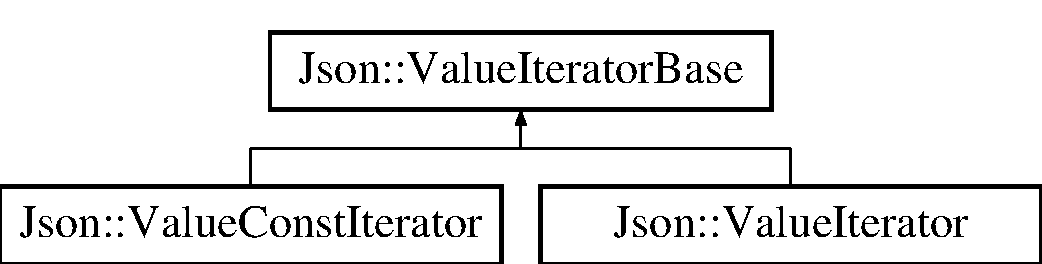
\includegraphics[height=2.000000cm]{classJson_1_1ValueIteratorBase}
\end{center}
\end{figure}
\subsection*{Public Types}
\begin{DoxyCompactItemize}
\item 
typedef std\+::bidirectional\+\_\+iterator\+\_\+tag \hyperlink{classJson_1_1ValueIteratorBase_a02fd11a4fbdc0007da1e8bcf5e6b83c3}{iterator\+\_\+category}
\item 
typedef unsigned int \hyperlink{classJson_1_1ValueIteratorBase_a9d3a3c7ce5cdefe23cb486239cf07bb5}{size\+\_\+t}
\item 
typedef int \hyperlink{classJson_1_1ValueIteratorBase_a4e44bf8cbd17ec8d6e2c185904a15ebd}{difference\+\_\+type}
\item 
typedef \hyperlink{classJson_1_1ValueIteratorBase}{Value\+Iterator\+Base} \hyperlink{classJson_1_1ValueIteratorBase_a9d2a940d03ea06d20d972f41a89149ee}{Self\+Type}
\end{DoxyCompactItemize}
\subsection*{Public Member Functions}
\begin{DoxyCompactItemize}
\item 
bool \hyperlink{classJson_1_1ValueIteratorBase_afc656672ac28502f640ade32c38c1b56}{operator==} (const \hyperlink{classJson_1_1ValueIteratorBase_a9d2a940d03ea06d20d972f41a89149ee}{Self\+Type} \&other) const 
\item 
bool \hyperlink{classJson_1_1ValueIteratorBase_a18c2dd42e0bb989ace141bfe9de52792}{operator!=} (const \hyperlink{classJson_1_1ValueIteratorBase_a9d2a940d03ea06d20d972f41a89149ee}{Self\+Type} \&other) const 
\item 
\hyperlink{classJson_1_1ValueIteratorBase_a4e44bf8cbd17ec8d6e2c185904a15ebd}{difference\+\_\+type} \hyperlink{classJson_1_1ValueIteratorBase_ab786787fcad68ca5e8745aaf520fa17f}{operator-\/} (const \hyperlink{classJson_1_1ValueIteratorBase_a9d2a940d03ea06d20d972f41a89149ee}{Self\+Type} \&other) const 
\item 
\hyperlink{classJson_1_1Value}{Value} \hyperlink{classJson_1_1ValueIteratorBase_aa2ff5e79fc96acd4c3cd288e92614fc7}{key} () const 
\begin{DoxyCompactList}\small\item\em Return either the index or the member name of the referenced value as a \hyperlink{classJson_1_1Value}{Value}. \end{DoxyCompactList}\item 
\hyperlink{namespaceJson_a800fb90eb6ee8d5d62b600c06f87f7d4}{U\+Int} \hyperlink{classJson_1_1ValueIteratorBase_aa90591f5f7f8d2f06cc4605816b53738}{index} () const 
\begin{DoxyCompactList}\small\item\em Return the index of the referenced \hyperlink{classJson_1_1Value}{Value}, or -\/1 if it is not an array\+Value. \end{DoxyCompactList}\item 
\hyperlink{json_8hpp_a1e723f95759de062585bc4a8fd3fa4be}{J\+S\+O\+N\+C\+P\+P\+\_\+\+S\+T\+R\+I\+NG} \hyperlink{classJson_1_1ValueIteratorBase_a99026427eb156ce007ef94df002e233f}{name} () const 
\begin{DoxyCompactList}\small\item\em Return the member name of the referenced \hyperlink{classJson_1_1Value}{Value}, or \char`\"{}\char`\"{} if it is not an object\+Value. \end{DoxyCompactList}\item 
char const $\ast$ \hyperlink{classJson_1_1ValueIteratorBase_ac3aa3870761342e47c6486d81f643c6c}{member\+Name} () const 
\begin{DoxyCompactList}\small\item\em Return the member name of the referenced \hyperlink{classJson_1_1Value}{Value}. \end{DoxyCompactList}\item 
char const $\ast$ \hyperlink{classJson_1_1ValueIteratorBase_a543d4e73e3d2d121bc287b24231386c3}{member\+Name} (char const $\ast$$\ast$end) const 
\begin{DoxyCompactList}\small\item\em Return the member name of the referenced \hyperlink{classJson_1_1Value}{Value}, or N\+U\+LL if it is not an object\+Value. \end{DoxyCompactList}\item 
\hyperlink{classJson_1_1ValueIteratorBase_af45b028d9ff9cbd2554a87878b42dd75}{Value\+Iterator\+Base} ()
\item 
\hyperlink{classJson_1_1ValueIteratorBase_a640e990e5f03a96fd650122a2906f59d}{Value\+Iterator\+Base} (const Value\+::\+Object\+Values\+::iterator \&current)
\end{DoxyCompactItemize}
\subsection*{Protected Member Functions}
\begin{DoxyCompactItemize}
\item 
\hyperlink{classJson_1_1Value}{Value} \& \hyperlink{classJson_1_1ValueIteratorBase_a40a20c65abc423a26e3aae68d9a0525c}{deref} () const 
\item 
void \hyperlink{classJson_1_1ValueIteratorBase_afe58f9534e1fd2033419fd9fe244551e}{increment} ()
\item 
void \hyperlink{classJson_1_1ValueIteratorBase_affc8cf5ff54a9f432cc693362c153fa6}{decrement} ()
\item 
\hyperlink{classJson_1_1ValueIteratorBase_a4e44bf8cbd17ec8d6e2c185904a15ebd}{difference\+\_\+type} \hyperlink{classJson_1_1ValueIteratorBase_ad6c553b249e89e3dc9933e100ccbe064}{compute\+Distance} (const \hyperlink{classJson_1_1ValueIteratorBase_a9d2a940d03ea06d20d972f41a89149ee}{Self\+Type} \&other) const 
\item 
bool \hyperlink{classJson_1_1ValueIteratorBase_a21820d6ee564e541bd118b21e4741962}{is\+Equal} (const \hyperlink{classJson_1_1ValueIteratorBase_a9d2a940d03ea06d20d972f41a89149ee}{Self\+Type} \&other) const 
\item 
void \hyperlink{classJson_1_1ValueIteratorBase_a496e6aba44808433ec5858c178be5719}{copy} (const \hyperlink{classJson_1_1ValueIteratorBase_a9d2a940d03ea06d20d972f41a89149ee}{Self\+Type} \&other)
\end{DoxyCompactItemize}
\subsection*{Private Attributes}
\begin{DoxyCompactItemize}
\item 
Value\+::\+Object\+Values\+::iterator \hyperlink{classJson_1_1ValueIteratorBase_ab3138ce8af8301cca3b041ea55cb922a}{current\+\_\+}
\item 
bool \hyperlink{classJson_1_1ValueIteratorBase_a3e08b114a1aed9bde518c527f94a8c59}{is\+Null\+\_\+}
\end{DoxyCompactItemize}


\subsection{Detailed Description}
base class for \hyperlink{classJson_1_1Value}{Value} iterators. 

\subsection{Member Typedef Documentation}
\index{Json\+::\+Value\+Iterator\+Base@{Json\+::\+Value\+Iterator\+Base}!difference\+\_\+type@{difference\+\_\+type}}
\index{difference\+\_\+type@{difference\+\_\+type}!Json\+::\+Value\+Iterator\+Base@{Json\+::\+Value\+Iterator\+Base}}
\subsubsection[{\texorpdfstring{difference\+\_\+type}{difference_type}}]{\setlength{\rightskip}{0pt plus 5cm}typedef int {\bf Json\+::\+Value\+Iterator\+Base\+::difference\+\_\+type}}\hypertarget{classJson_1_1ValueIteratorBase_a4e44bf8cbd17ec8d6e2c185904a15ebd}{}\label{classJson_1_1ValueIteratorBase_a4e44bf8cbd17ec8d6e2c185904a15ebd}
\index{Json\+::\+Value\+Iterator\+Base@{Json\+::\+Value\+Iterator\+Base}!iterator\+\_\+category@{iterator\+\_\+category}}
\index{iterator\+\_\+category@{iterator\+\_\+category}!Json\+::\+Value\+Iterator\+Base@{Json\+::\+Value\+Iterator\+Base}}
\subsubsection[{\texorpdfstring{iterator\+\_\+category}{iterator_category}}]{\setlength{\rightskip}{0pt plus 5cm}typedef std\+::bidirectional\+\_\+iterator\+\_\+tag {\bf Json\+::\+Value\+Iterator\+Base\+::iterator\+\_\+category}}\hypertarget{classJson_1_1ValueIteratorBase_a02fd11a4fbdc0007da1e8bcf5e6b83c3}{}\label{classJson_1_1ValueIteratorBase_a02fd11a4fbdc0007da1e8bcf5e6b83c3}
\index{Json\+::\+Value\+Iterator\+Base@{Json\+::\+Value\+Iterator\+Base}!Self\+Type@{Self\+Type}}
\index{Self\+Type@{Self\+Type}!Json\+::\+Value\+Iterator\+Base@{Json\+::\+Value\+Iterator\+Base}}
\subsubsection[{\texorpdfstring{Self\+Type}{SelfType}}]{\setlength{\rightskip}{0pt plus 5cm}typedef {\bf Value\+Iterator\+Base} {\bf Json\+::\+Value\+Iterator\+Base\+::\+Self\+Type}}\hypertarget{classJson_1_1ValueIteratorBase_a9d2a940d03ea06d20d972f41a89149ee}{}\label{classJson_1_1ValueIteratorBase_a9d2a940d03ea06d20d972f41a89149ee}
\index{Json\+::\+Value\+Iterator\+Base@{Json\+::\+Value\+Iterator\+Base}!size\+\_\+t@{size\+\_\+t}}
\index{size\+\_\+t@{size\+\_\+t}!Json\+::\+Value\+Iterator\+Base@{Json\+::\+Value\+Iterator\+Base}}
\subsubsection[{\texorpdfstring{size\+\_\+t}{size_t}}]{\setlength{\rightskip}{0pt plus 5cm}typedef unsigned int {\bf Json\+::\+Value\+Iterator\+Base\+::size\+\_\+t}}\hypertarget{classJson_1_1ValueIteratorBase_a9d3a3c7ce5cdefe23cb486239cf07bb5}{}\label{classJson_1_1ValueIteratorBase_a9d3a3c7ce5cdefe23cb486239cf07bb5}


\subsection{Constructor \& Destructor Documentation}
\index{Json\+::\+Value\+Iterator\+Base@{Json\+::\+Value\+Iterator\+Base}!Value\+Iterator\+Base@{Value\+Iterator\+Base}}
\index{Value\+Iterator\+Base@{Value\+Iterator\+Base}!Json\+::\+Value\+Iterator\+Base@{Json\+::\+Value\+Iterator\+Base}}
\subsubsection[{\texorpdfstring{Value\+Iterator\+Base()}{ValueIteratorBase()}}]{\setlength{\rightskip}{0pt plus 5cm}Json\+::\+Value\+Iterator\+Base\+::\+Value\+Iterator\+Base (
\begin{DoxyParamCaption}
{}
\end{DoxyParamCaption}
)}\hypertarget{classJson_1_1ValueIteratorBase_af45b028d9ff9cbd2554a87878b42dd75}{}\label{classJson_1_1ValueIteratorBase_af45b028d9ff9cbd2554a87878b42dd75}
\index{Json\+::\+Value\+Iterator\+Base@{Json\+::\+Value\+Iterator\+Base}!Value\+Iterator\+Base@{Value\+Iterator\+Base}}
\index{Value\+Iterator\+Base@{Value\+Iterator\+Base}!Json\+::\+Value\+Iterator\+Base@{Json\+::\+Value\+Iterator\+Base}}
\subsubsection[{\texorpdfstring{Value\+Iterator\+Base(const Value\+::\+Object\+Values\+::iterator \&current)}{ValueIteratorBase(const Value::ObjectValues::iterator &current)}}]{\setlength{\rightskip}{0pt plus 5cm}Json\+::\+Value\+Iterator\+Base\+::\+Value\+Iterator\+Base (
\begin{DoxyParamCaption}
\item[{const Value\+::\+Object\+Values\+::iterator \&}]{current}
\end{DoxyParamCaption}
)\hspace{0.3cm}{\ttfamily [explicit]}}\hypertarget{classJson_1_1ValueIteratorBase_a640e990e5f03a96fd650122a2906f59d}{}\label{classJson_1_1ValueIteratorBase_a640e990e5f03a96fd650122a2906f59d}


\subsection{Member Function Documentation}
\index{Json\+::\+Value\+Iterator\+Base@{Json\+::\+Value\+Iterator\+Base}!compute\+Distance@{compute\+Distance}}
\index{compute\+Distance@{compute\+Distance}!Json\+::\+Value\+Iterator\+Base@{Json\+::\+Value\+Iterator\+Base}}
\subsubsection[{\texorpdfstring{compute\+Distance(const Self\+Type \&other) const }{computeDistance(const SelfType &other) const }}]{\setlength{\rightskip}{0pt plus 5cm}{\bf Value\+Iterator\+Base\+::difference\+\_\+type} Json\+::\+Value\+Iterator\+Base\+::compute\+Distance (
\begin{DoxyParamCaption}
\item[{const {\bf Self\+Type} \&}]{other}
\end{DoxyParamCaption}
) const\hspace{0.3cm}{\ttfamily [protected]}}\hypertarget{classJson_1_1ValueIteratorBase_ad6c553b249e89e3dc9933e100ccbe064}{}\label{classJson_1_1ValueIteratorBase_ad6c553b249e89e3dc9933e100ccbe064}
\index{Json\+::\+Value\+Iterator\+Base@{Json\+::\+Value\+Iterator\+Base}!copy@{copy}}
\index{copy@{copy}!Json\+::\+Value\+Iterator\+Base@{Json\+::\+Value\+Iterator\+Base}}
\subsubsection[{\texorpdfstring{copy(const Self\+Type \&other)}{copy(const SelfType &other)}}]{\setlength{\rightskip}{0pt plus 5cm}void Json\+::\+Value\+Iterator\+Base\+::copy (
\begin{DoxyParamCaption}
\item[{const {\bf Self\+Type} \&}]{other}
\end{DoxyParamCaption}
)\hspace{0.3cm}{\ttfamily [protected]}}\hypertarget{classJson_1_1ValueIteratorBase_a496e6aba44808433ec5858c178be5719}{}\label{classJson_1_1ValueIteratorBase_a496e6aba44808433ec5858c178be5719}
\index{Json\+::\+Value\+Iterator\+Base@{Json\+::\+Value\+Iterator\+Base}!decrement@{decrement}}
\index{decrement@{decrement}!Json\+::\+Value\+Iterator\+Base@{Json\+::\+Value\+Iterator\+Base}}
\subsubsection[{\texorpdfstring{decrement()}{decrement()}}]{\setlength{\rightskip}{0pt plus 5cm}void Json\+::\+Value\+Iterator\+Base\+::decrement (
\begin{DoxyParamCaption}
{}
\end{DoxyParamCaption}
)\hspace{0.3cm}{\ttfamily [protected]}}\hypertarget{classJson_1_1ValueIteratorBase_affc8cf5ff54a9f432cc693362c153fa6}{}\label{classJson_1_1ValueIteratorBase_affc8cf5ff54a9f432cc693362c153fa6}
\index{Json\+::\+Value\+Iterator\+Base@{Json\+::\+Value\+Iterator\+Base}!deref@{deref}}
\index{deref@{deref}!Json\+::\+Value\+Iterator\+Base@{Json\+::\+Value\+Iterator\+Base}}
\subsubsection[{\texorpdfstring{deref() const }{deref() const }}]{\setlength{\rightskip}{0pt plus 5cm}{\bf Value} \& Json\+::\+Value\+Iterator\+Base\+::deref (
\begin{DoxyParamCaption}
{}
\end{DoxyParamCaption}
) const\hspace{0.3cm}{\ttfamily [protected]}}\hypertarget{classJson_1_1ValueIteratorBase_a40a20c65abc423a26e3aae68d9a0525c}{}\label{classJson_1_1ValueIteratorBase_a40a20c65abc423a26e3aae68d9a0525c}
\index{Json\+::\+Value\+Iterator\+Base@{Json\+::\+Value\+Iterator\+Base}!increment@{increment}}
\index{increment@{increment}!Json\+::\+Value\+Iterator\+Base@{Json\+::\+Value\+Iterator\+Base}}
\subsubsection[{\texorpdfstring{increment()}{increment()}}]{\setlength{\rightskip}{0pt plus 5cm}void Json\+::\+Value\+Iterator\+Base\+::increment (
\begin{DoxyParamCaption}
{}
\end{DoxyParamCaption}
)\hspace{0.3cm}{\ttfamily [protected]}}\hypertarget{classJson_1_1ValueIteratorBase_afe58f9534e1fd2033419fd9fe244551e}{}\label{classJson_1_1ValueIteratorBase_afe58f9534e1fd2033419fd9fe244551e}
\index{Json\+::\+Value\+Iterator\+Base@{Json\+::\+Value\+Iterator\+Base}!index@{index}}
\index{index@{index}!Json\+::\+Value\+Iterator\+Base@{Json\+::\+Value\+Iterator\+Base}}
\subsubsection[{\texorpdfstring{index() const }{index() const }}]{\setlength{\rightskip}{0pt plus 5cm}{\bf U\+Int} Json\+::\+Value\+Iterator\+Base\+::index (
\begin{DoxyParamCaption}
{}
\end{DoxyParamCaption}
) const}\hypertarget{classJson_1_1ValueIteratorBase_aa90591f5f7f8d2f06cc4605816b53738}{}\label{classJson_1_1ValueIteratorBase_aa90591f5f7f8d2f06cc4605816b53738}


Return the index of the referenced \hyperlink{classJson_1_1Value}{Value}, or -\/1 if it is not an array\+Value. 

\index{Json\+::\+Value\+Iterator\+Base@{Json\+::\+Value\+Iterator\+Base}!is\+Equal@{is\+Equal}}
\index{is\+Equal@{is\+Equal}!Json\+::\+Value\+Iterator\+Base@{Json\+::\+Value\+Iterator\+Base}}
\subsubsection[{\texorpdfstring{is\+Equal(const Self\+Type \&other) const }{isEqual(const SelfType &other) const }}]{\setlength{\rightskip}{0pt plus 5cm}bool Json\+::\+Value\+Iterator\+Base\+::is\+Equal (
\begin{DoxyParamCaption}
\item[{const {\bf Self\+Type} \&}]{other}
\end{DoxyParamCaption}
) const\hspace{0.3cm}{\ttfamily [protected]}}\hypertarget{classJson_1_1ValueIteratorBase_a21820d6ee564e541bd118b21e4741962}{}\label{classJson_1_1ValueIteratorBase_a21820d6ee564e541bd118b21e4741962}
\index{Json\+::\+Value\+Iterator\+Base@{Json\+::\+Value\+Iterator\+Base}!key@{key}}
\index{key@{key}!Json\+::\+Value\+Iterator\+Base@{Json\+::\+Value\+Iterator\+Base}}
\subsubsection[{\texorpdfstring{key() const }{key() const }}]{\setlength{\rightskip}{0pt plus 5cm}{\bf Value} Json\+::\+Value\+Iterator\+Base\+::key (
\begin{DoxyParamCaption}
{}
\end{DoxyParamCaption}
) const}\hypertarget{classJson_1_1ValueIteratorBase_aa2ff5e79fc96acd4c3cd288e92614fc7}{}\label{classJson_1_1ValueIteratorBase_aa2ff5e79fc96acd4c3cd288e92614fc7}


Return either the index or the member name of the referenced value as a \hyperlink{classJson_1_1Value}{Value}. 

\index{Json\+::\+Value\+Iterator\+Base@{Json\+::\+Value\+Iterator\+Base}!member\+Name@{member\+Name}}
\index{member\+Name@{member\+Name}!Json\+::\+Value\+Iterator\+Base@{Json\+::\+Value\+Iterator\+Base}}
\subsubsection[{\texorpdfstring{member\+Name() const }{memberName() const }}]{\setlength{\rightskip}{0pt plus 5cm}char const $\ast$ Json\+::\+Value\+Iterator\+Base\+::member\+Name (
\begin{DoxyParamCaption}
{}
\end{DoxyParamCaption}
) const}\hypertarget{classJson_1_1ValueIteratorBase_ac3aa3870761342e47c6486d81f643c6c}{}\label{classJson_1_1ValueIteratorBase_ac3aa3870761342e47c6486d81f643c6c}


Return the member name of the referenced \hyperlink{classJson_1_1Value}{Value}. 

\char`\"{}\char`\"{} if it is not an object\+Value. \begin{DoxyRefDesc}{Deprecated}
\item[\hyperlink{deprecated__deprecated000004}{Deprecated}]This cannot be used for U\+T\+F-\/8 strings, since there can be embedded nulls. \end{DoxyRefDesc}
\index{Json\+::\+Value\+Iterator\+Base@{Json\+::\+Value\+Iterator\+Base}!member\+Name@{member\+Name}}
\index{member\+Name@{member\+Name}!Json\+::\+Value\+Iterator\+Base@{Json\+::\+Value\+Iterator\+Base}}
\subsubsection[{\texorpdfstring{member\+Name(char const $\ast$$\ast$end) const }{memberName(char const **end) const }}]{\setlength{\rightskip}{0pt plus 5cm}char const $\ast$ Json\+::\+Value\+Iterator\+Base\+::member\+Name (
\begin{DoxyParamCaption}
\item[{char const $\ast$$\ast$}]{end}
\end{DoxyParamCaption}
) const}\hypertarget{classJson_1_1ValueIteratorBase_a543d4e73e3d2d121bc287b24231386c3}{}\label{classJson_1_1ValueIteratorBase_a543d4e73e3d2d121bc287b24231386c3}


Return the member name of the referenced \hyperlink{classJson_1_1Value}{Value}, or N\+U\+LL if it is not an object\+Value. 

\begin{DoxyNote}{Note}
Better version than \hyperlink{classJson_1_1ValueIteratorBase_ac3aa3870761342e47c6486d81f643c6c}{member\+Name()}. Allows embedded nulls. 
\end{DoxyNote}
\index{Json\+::\+Value\+Iterator\+Base@{Json\+::\+Value\+Iterator\+Base}!name@{name}}
\index{name@{name}!Json\+::\+Value\+Iterator\+Base@{Json\+::\+Value\+Iterator\+Base}}
\subsubsection[{\texorpdfstring{name() const }{name() const }}]{\setlength{\rightskip}{0pt plus 5cm}{\bf J\+S\+O\+N\+C\+P\+P\+\_\+\+S\+T\+R\+I\+NG} Json\+::\+Value\+Iterator\+Base\+::name (
\begin{DoxyParamCaption}
{}
\end{DoxyParamCaption}
) const}\hypertarget{classJson_1_1ValueIteratorBase_a99026427eb156ce007ef94df002e233f}{}\label{classJson_1_1ValueIteratorBase_a99026427eb156ce007ef94df002e233f}


Return the member name of the referenced \hyperlink{classJson_1_1Value}{Value}, or \char`\"{}\char`\"{} if it is not an object\+Value. 

\begin{DoxyNote}{Note}
Avoid {\ttfamily c\+\_\+str()} on result, as embedded zeroes are possible. 
\end{DoxyNote}
\index{Json\+::\+Value\+Iterator\+Base@{Json\+::\+Value\+Iterator\+Base}!operator"!=@{operator"!=}}
\index{operator"!=@{operator"!=}!Json\+::\+Value\+Iterator\+Base@{Json\+::\+Value\+Iterator\+Base}}
\subsubsection[{\texorpdfstring{operator"!=(const Self\+Type \&other) const }{operator!=(const SelfType &other) const }}]{\setlength{\rightskip}{0pt plus 5cm}bool Json\+::\+Value\+Iterator\+Base\+::operator!= (
\begin{DoxyParamCaption}
\item[{const {\bf Self\+Type} \&}]{other}
\end{DoxyParamCaption}
) const\hspace{0.3cm}{\ttfamily [inline]}}\hypertarget{classJson_1_1ValueIteratorBase_a18c2dd42e0bb989ace141bfe9de52792}{}\label{classJson_1_1ValueIteratorBase_a18c2dd42e0bb989ace141bfe9de52792}
\index{Json\+::\+Value\+Iterator\+Base@{Json\+::\+Value\+Iterator\+Base}!operator-\/@{operator-\/}}
\index{operator-\/@{operator-\/}!Json\+::\+Value\+Iterator\+Base@{Json\+::\+Value\+Iterator\+Base}}
\subsubsection[{\texorpdfstring{operator-\/(const Self\+Type \&other) const }{operator-(const SelfType &other) const }}]{\setlength{\rightskip}{0pt plus 5cm}{\bf difference\+\_\+type} Json\+::\+Value\+Iterator\+Base\+::operator-\/ (
\begin{DoxyParamCaption}
\item[{const {\bf Self\+Type} \&}]{other}
\end{DoxyParamCaption}
) const\hspace{0.3cm}{\ttfamily [inline]}}\hypertarget{classJson_1_1ValueIteratorBase_ab786787fcad68ca5e8745aaf520fa17f}{}\label{classJson_1_1ValueIteratorBase_ab786787fcad68ca5e8745aaf520fa17f}
\index{Json\+::\+Value\+Iterator\+Base@{Json\+::\+Value\+Iterator\+Base}!operator==@{operator==}}
\index{operator==@{operator==}!Json\+::\+Value\+Iterator\+Base@{Json\+::\+Value\+Iterator\+Base}}
\subsubsection[{\texorpdfstring{operator==(const Self\+Type \&other) const }{operator==(const SelfType &other) const }}]{\setlength{\rightskip}{0pt plus 5cm}bool Json\+::\+Value\+Iterator\+Base\+::operator== (
\begin{DoxyParamCaption}
\item[{const {\bf Self\+Type} \&}]{other}
\end{DoxyParamCaption}
) const\hspace{0.3cm}{\ttfamily [inline]}}\hypertarget{classJson_1_1ValueIteratorBase_afc656672ac28502f640ade32c38c1b56}{}\label{classJson_1_1ValueIteratorBase_afc656672ac28502f640ade32c38c1b56}


\subsection{Member Data Documentation}
\index{Json\+::\+Value\+Iterator\+Base@{Json\+::\+Value\+Iterator\+Base}!current\+\_\+@{current\+\_\+}}
\index{current\+\_\+@{current\+\_\+}!Json\+::\+Value\+Iterator\+Base@{Json\+::\+Value\+Iterator\+Base}}
\subsubsection[{\texorpdfstring{current\+\_\+}{current_}}]{\setlength{\rightskip}{0pt plus 5cm}Value\+::\+Object\+Values\+::iterator Json\+::\+Value\+Iterator\+Base\+::current\+\_\+\hspace{0.3cm}{\ttfamily [private]}}\hypertarget{classJson_1_1ValueIteratorBase_ab3138ce8af8301cca3b041ea55cb922a}{}\label{classJson_1_1ValueIteratorBase_ab3138ce8af8301cca3b041ea55cb922a}
\index{Json\+::\+Value\+Iterator\+Base@{Json\+::\+Value\+Iterator\+Base}!is\+Null\+\_\+@{is\+Null\+\_\+}}
\index{is\+Null\+\_\+@{is\+Null\+\_\+}!Json\+::\+Value\+Iterator\+Base@{Json\+::\+Value\+Iterator\+Base}}
\subsubsection[{\texorpdfstring{is\+Null\+\_\+}{isNull_}}]{\setlength{\rightskip}{0pt plus 5cm}bool Json\+::\+Value\+Iterator\+Base\+::is\+Null\+\_\+\hspace{0.3cm}{\ttfamily [private]}}\hypertarget{classJson_1_1ValueIteratorBase_a3e08b114a1aed9bde518c527f94a8c59}{}\label{classJson_1_1ValueIteratorBase_a3e08b114a1aed9bde518c527f94a8c59}


The documentation for this class was generated from the following files\+:\begin{DoxyCompactItemize}
\item 
/home/pranav/\+Repositories/zcm/include/\hyperlink{json_8hpp}{json.\+hpp}\item 
/home/pranav/\+Repositories/zcm/src/\hyperlink{json_8cpp}{json.\+cpp}\end{DoxyCompactItemize}

\hypertarget{classJson_1_1Writer}{}\section{Json\+:\+:Writer Class Reference}
\label{classJson_1_1Writer}\index{Json\+::\+Writer@{Json\+::\+Writer}}


Abstract class for writers.  




{\ttfamily \#include $<$json.\+hpp$>$}

Inheritance diagram for Json\+:\+:Writer\+:\begin{figure}[H]
\begin{center}
\leavevmode
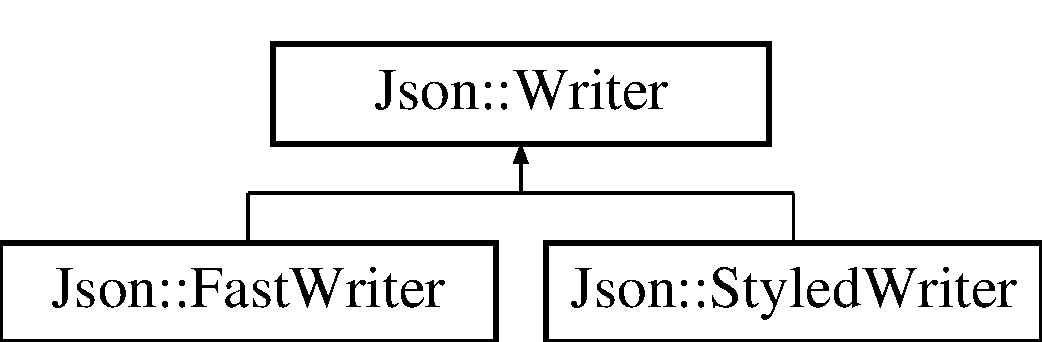
\includegraphics[height=2.000000cm]{classJson_1_1Writer}
\end{center}
\end{figure}
\subsection*{Public Member Functions}
\begin{DoxyCompactItemize}
\item 
virtual \hyperlink{classJson_1_1Writer_a3e618564336f26b14921f0d840db668c}{$\sim$\+Writer} ()
\item 
virtual \hyperlink{json_8hpp_a1e723f95759de062585bc4a8fd3fa4be}{J\+S\+O\+N\+C\+P\+P\+\_\+\+S\+T\+R\+I\+NG} \hyperlink{classJson_1_1Writer_a61c55882b82c7651d0b9b683c6d3f371}{write} (const \hyperlink{classJson_1_1Value}{Value} \&root)=0
\end{DoxyCompactItemize}


\subsection{Detailed Description}
Abstract class for writers. 

\begin{DoxyRefDesc}{Deprecated}
\item[\hyperlink{deprecated__deprecated000007}{Deprecated}]Use \hyperlink{classJson_1_1StreamWriter}{Stream\+Writer}. (And really, this is an implementation detail.) \end{DoxyRefDesc}


\subsection{Constructor \& Destructor Documentation}
\index{Json\+::\+Writer@{Json\+::\+Writer}!````~Writer@{$\sim$\+Writer}}
\index{````~Writer@{$\sim$\+Writer}!Json\+::\+Writer@{Json\+::\+Writer}}
\subsubsection[{\texorpdfstring{$\sim$\+Writer()}{~Writer()}}]{\setlength{\rightskip}{0pt plus 5cm}Json\+::\+Writer\+::$\sim$\+Writer (
\begin{DoxyParamCaption}
{}
\end{DoxyParamCaption}
)\hspace{0.3cm}{\ttfamily [virtual]}}\hypertarget{classJson_1_1Writer_a3e618564336f26b14921f0d840db668c}{}\label{classJson_1_1Writer_a3e618564336f26b14921f0d840db668c}


\subsection{Member Function Documentation}
\index{Json\+::\+Writer@{Json\+::\+Writer}!write@{write}}
\index{write@{write}!Json\+::\+Writer@{Json\+::\+Writer}}
\subsubsection[{\texorpdfstring{write(const Value \&root)=0}{write(const Value &root)=0}}]{\setlength{\rightskip}{0pt plus 5cm}virtual {\bf J\+S\+O\+N\+C\+P\+P\+\_\+\+S\+T\+R\+I\+NG} Json\+::\+Writer\+::write (
\begin{DoxyParamCaption}
\item[{const {\bf Value} \&}]{root}
\end{DoxyParamCaption}
)\hspace{0.3cm}{\ttfamily [pure virtual]}}\hypertarget{classJson_1_1Writer_a61c55882b82c7651d0b9b683c6d3f371}{}\label{classJson_1_1Writer_a61c55882b82c7651d0b9b683c6d3f371}


Implemented in \hyperlink{classJson_1_1StyledWriter_a5efab19b9746da9920c29cdae3a6b404}{Json\+::\+Styled\+Writer}, and \hyperlink{classJson_1_1FastWriter_a93d45ba4bc312371d08beb3e3dfbe654}{Json\+::\+Fast\+Writer}.



The documentation for this class was generated from the following files\+:\begin{DoxyCompactItemize}
\item 
/home/pranav/\+Repositories/zcm/include/\hyperlink{json_8hpp}{json.\+hpp}\item 
/home/pranav/\+Repositories/zcm/src/\hyperlink{json_8cpp}{json.\+cpp}\end{DoxyCompactItemize}

\chapter{File Documentation}
\hypertarget{actor_8hpp}{\section{/home/kelsier/\-Git\-Hub/zcm/include/actor.hpp File Reference}
\label{actor_8hpp}\index{/home/kelsier/\-Git\-Hub/zcm/include/actor.\-hpp@{/home/kelsier/\-Git\-Hub/zcm/include/actor.\-hpp}}
}


This file declares the Actor class.  


{\ttfamily \#include \char`\"{}json.\-hpp\char`\"{}}\\*
{\ttfamily \#include \char`\"{}component.\-hpp\char`\"{}}\\*
{\ttfamily \#include $<$dlfcn.\-h$>$}\\*
{\ttfamily \#include $<$fstream$>$}\\*
\subsection*{Classes}
\begin{DoxyCompactItemize}
\item 
class \hyperlink{classzcm_1_1Actor}{zcm\-::\-Actor}
\begin{DoxyCompactList}\small\item\em \hyperlink{classzcm_1_1Actor}{Actor} class. \end{DoxyCompactList}\end{DoxyCompactItemize}
\subsection*{Namespaces}
\begin{DoxyCompactItemize}
\item 
\hyperlink{namespacezcm}{zcm}
\end{DoxyCompactItemize}


\subsection{Detailed Description}
This file declares the Actor class. \begin{DoxyAuthor}{Author}
Pranav Srinivas Kumar 
\end{DoxyAuthor}
\begin{DoxyDate}{Date}
2016.\-04.\-24 
\end{DoxyDate}

\hypertarget{client_8hpp}{}\section{/home/pranav/\+Repositories/zcm/include/client.hpp File Reference}
\label{client_8hpp}\index{/home/pranav/\+Repositories/zcm/include/client.\+hpp@{/home/pranav/\+Repositories/zcm/include/client.\+hpp}}


This file declares the Client class.  


{\ttfamily \#include $<$iostream$>$}\\*
{\ttfamily \#include $<$zmq.\+hpp$>$}\\*
\subsection*{Classes}
\begin{DoxyCompactItemize}
\item 
class \hyperlink{classzcm_1_1Client}{zcm\+::\+Client}
\begin{DoxyCompactList}\small\item\em \hyperlink{classzcm_1_1Client}{Client} class. \end{DoxyCompactList}\end{DoxyCompactItemize}
\subsection*{Namespaces}
\begin{DoxyCompactItemize}
\item 
 \hyperlink{namespacezcm}{zcm}
\end{DoxyCompactItemize}


\subsection{Detailed Description}
This file declares the Client class. 

\begin{DoxyAuthor}{Author}
Pranav Srinivas Kumar 
\end{DoxyAuthor}
\begin{DoxyDate}{Date}
2016.\+04.\+24 
\end{DoxyDate}

\hypertarget{component_8hpp}{\section{/home/kelsier/\-Git\-Hub/zcm/include/component.hpp File Reference}
\label{component_8hpp}\index{/home/kelsier/\-Git\-Hub/zcm/include/component.\-hpp@{/home/kelsier/\-Git\-Hub/zcm/include/component.\-hpp}}
}


This file declares the Component class.  


{\ttfamily \#include \char`\"{}timer.\-hpp\char`\"{}}\\*
{\ttfamily \#include \char`\"{}publisher.\-hpp\char`\"{}}\\*
{\ttfamily \#include \char`\"{}subscriber.\-hpp\char`\"{}}\\*
{\ttfamily \#include \char`\"{}client.\-hpp\char`\"{}}\\*
{\ttfamily \#include \char`\"{}server.\-hpp\char`\"{}}\\*
\subsection*{Classes}
\begin{DoxyCompactItemize}
\item 
class \hyperlink{classzcm_1_1Component}{zcm\-::\-Component}
\begin{DoxyCompactList}\small\item\em \hyperlink{classzcm_1_1Component}{Component} class. \end{DoxyCompactList}\end{DoxyCompactItemize}
\subsection*{Namespaces}
\begin{DoxyCompactItemize}
\item 
\hyperlink{namespacezcm}{zcm}
\end{DoxyCompactItemize}


\subsection{Detailed Description}
This file declares the Component class. \begin{DoxyAuthor}{Author}
Pranav Srinivas Kumar 
\end{DoxyAuthor}
\begin{DoxyDate}{Date}
2016.\-04.\-24 
\end{DoxyDate}

\hypertarget{json_8hpp}{}\section{/home/pranav/\+Repositories/zcm/include/json.hpp File Reference}
\label{json_8hpp}\index{/home/pranav/\+Repositories/zcm/include/json.\+hpp@{/home/pranav/\+Repositories/zcm/include/json.\+hpp}}
{\ttfamily \#include $<$stddef.\+h$>$}\\*
{\ttfamily \#include $<$string$>$}\\*
{\ttfamily \#include $<$vector$>$}\\*
{\ttfamily \#include $<$exception$>$}\\*
{\ttfamily \#include $<$map$>$}\\*
{\ttfamily \#include $<$deque$>$}\\*
{\ttfamily \#include $<$iosfwd$>$}\\*
{\ttfamily \#include $<$stack$>$}\\*
{\ttfamily \#include $<$istream$>$}\\*
{\ttfamily \#include $<$ostream$>$}\\*
{\ttfamily \#include $<$stdlib.\+h$>$}\\*
{\ttfamily \#include $<$sstream$>$}\\*
\subsection*{Classes}
\begin{DoxyCompactItemize}
\item 
class \hyperlink{classJson_1_1Features}{Json\+::\+Features}
\begin{DoxyCompactList}\small\item\em Configuration passed to reader and writer. \end{DoxyCompactList}\item 
class \hyperlink{classJson_1_1Exception}{Json\+::\+Exception}
\begin{DoxyCompactList}\small\item\em Base class for all exceptions we throw. \end{DoxyCompactList}\item 
class \hyperlink{classJson_1_1RuntimeError}{Json\+::\+Runtime\+Error}
\begin{DoxyCompactList}\small\item\em Exceptions which the user cannot easily avoid. \end{DoxyCompactList}\item 
class \hyperlink{classJson_1_1LogicError}{Json\+::\+Logic\+Error}
\begin{DoxyCompactList}\small\item\em Exceptions thrown by J\+S\+O\+N\+\_\+\+A\+S\+S\+E\+R\+T/\+J\+S\+O\+N\+\_\+\+F\+A\+IL macros. \end{DoxyCompactList}\item 
class \hyperlink{classJson_1_1StaticString}{Json\+::\+Static\+String}
\begin{DoxyCompactList}\small\item\em Lightweight wrapper to tag static string. \end{DoxyCompactList}\item 
class \hyperlink{classJson_1_1Value}{Json\+::\+Value}
\begin{DoxyCompactList}\small\item\em Represents a \href{http://www.json.org}{\tt J\+S\+ON} value. \end{DoxyCompactList}\item 
class \hyperlink{classJson_1_1Value_1_1CZString}{Json\+::\+Value\+::\+C\+Z\+String}
\item 
struct \hyperlink{structJson_1_1Value_1_1CZString_1_1StringStorage}{Json\+::\+Value\+::\+C\+Z\+String\+::\+String\+Storage}
\item 
struct \hyperlink{structJson_1_1Value_1_1CommentInfo}{Json\+::\+Value\+::\+Comment\+Info}
\item 
union \hyperlink{unionJson_1_1Value_1_1ValueHolder}{Json\+::\+Value\+::\+Value\+Holder}
\item 
class \hyperlink{classJson_1_1PathArgument}{Json\+::\+Path\+Argument}
\begin{DoxyCompactList}\small\item\em Experimental and untested\+: represents an element of the \char`\"{}path\char`\"{} to access a node. \end{DoxyCompactList}\item 
class \hyperlink{classJson_1_1Path}{Json\+::\+Path}
\begin{DoxyCompactList}\small\item\em Experimental and untested\+: represents a \char`\"{}path\char`\"{} to access a node. \end{DoxyCompactList}\item 
class \hyperlink{classJson_1_1ValueIteratorBase}{Json\+::\+Value\+Iterator\+Base}
\begin{DoxyCompactList}\small\item\em base class for \hyperlink{classJson_1_1Value}{Value} iterators. \end{DoxyCompactList}\item 
class \hyperlink{classJson_1_1ValueConstIterator}{Json\+::\+Value\+Const\+Iterator}
\begin{DoxyCompactList}\small\item\em const iterator for object and array value. \end{DoxyCompactList}\item 
class \hyperlink{classJson_1_1ValueIterator}{Json\+::\+Value\+Iterator}
\begin{DoxyCompactList}\small\item\em Iterator for object and array value. \end{DoxyCompactList}\item 
class \hyperlink{classJson_1_1Reader}{Json\+::\+Reader}
\begin{DoxyCompactList}\small\item\em Unserialize a \href{http://www.json.org}{\tt J\+S\+ON} document into a \hyperlink{classJson_1_1Value}{Value}. \end{DoxyCompactList}\item 
struct \hyperlink{structJson_1_1Reader_1_1StructuredError}{Json\+::\+Reader\+::\+Structured\+Error}
\begin{DoxyCompactList}\small\item\em An error tagged with where in the J\+S\+ON text it was encountered. \end{DoxyCompactList}\item 
class \hyperlink{classJson_1_1Reader_1_1Token}{Json\+::\+Reader\+::\+Token}
\item 
class \hyperlink{classJson_1_1Reader_1_1ErrorInfo}{Json\+::\+Reader\+::\+Error\+Info}
\item 
class \hyperlink{classJson_1_1CharReader}{Json\+::\+Char\+Reader}
\begin{DoxyCompactList}\small\item\em Interface for reading J\+S\+ON from a char array. \end{DoxyCompactList}\item 
class \hyperlink{classJson_1_1CharReader_1_1Factory}{Json\+::\+Char\+Reader\+::\+Factory}
\item 
class \hyperlink{classJson_1_1CharReaderBuilder}{Json\+::\+Char\+Reader\+Builder}
\begin{DoxyCompactList}\small\item\em Build a \hyperlink{classJson_1_1CharReader}{Char\+Reader} implementation. \end{DoxyCompactList}\item 
class \hyperlink{classJson_1_1StreamWriter}{Json\+::\+Stream\+Writer}
\begin{DoxyCompactList}\small\item\em Usage\+: \end{DoxyCompactList}\item 
class \hyperlink{classJson_1_1StreamWriter_1_1Factory}{Json\+::\+Stream\+Writer\+::\+Factory}
\begin{DoxyCompactList}\small\item\em A simple abstract factory. \end{DoxyCompactList}\item 
class \hyperlink{classJson_1_1StreamWriterBuilder}{Json\+::\+Stream\+Writer\+Builder}
\begin{DoxyCompactList}\small\item\em Build a \hyperlink{classJson_1_1StreamWriter}{Stream\+Writer} implementation. \end{DoxyCompactList}\item 
class \hyperlink{classJson_1_1Writer}{Json\+::\+Writer}
\begin{DoxyCompactList}\small\item\em Abstract class for writers. \end{DoxyCompactList}\item 
class \hyperlink{classJson_1_1FastWriter}{Json\+::\+Fast\+Writer}
\begin{DoxyCompactList}\small\item\em Outputs a \hyperlink{classJson_1_1Value}{Value} in \href{http://www.json.org}{\tt J\+S\+ON} format without formatting (not human friendly). \end{DoxyCompactList}\item 
class \hyperlink{classJson_1_1StyledWriter}{Json\+::\+Styled\+Writer}
\begin{DoxyCompactList}\small\item\em Writes a \hyperlink{classJson_1_1Value}{Value} in \href{http://www.json.org}{\tt J\+S\+ON} format in a human friendly way. \end{DoxyCompactList}\item 
class \hyperlink{classJson_1_1StyledStreamWriter}{Json\+::\+Styled\+Stream\+Writer}
\begin{DoxyCompactList}\small\item\em Writes a \hyperlink{classJson_1_1Value}{Value} in \href{http://www.json.org}{\tt J\+S\+ON} format in a human friendly way, to a stream rather than to a string. \end{DoxyCompactList}\end{DoxyCompactItemize}
\subsection*{Namespaces}
\begin{DoxyCompactItemize}
\item 
 \hyperlink{namespaceJson}{Json}
\begin{DoxyCompactList}\small\item\em J\+S\+ON (Java\+Script Object Notation). \end{DoxyCompactList}\item 
 \hyperlink{namespacestd}{std}
\end{DoxyCompactItemize}
\subsection*{Macros}
\begin{DoxyCompactItemize}
\item 
\#define \hyperlink{json_8hpp_a1bf16856b5e907aa83ed7bc825bc5ecf}{J\+S\+O\+N\+\_\+\+I\+S\+\_\+\+A\+M\+A\+L\+G\+A\+M\+A\+T\+I\+ON}
\begin{DoxyCompactList}\small\item\em Json-\/cpp amalgated header (\href{http://jsoncpp.sourceforge.net/}{\tt http\+://jsoncpp.\+sourceforge.\+net/}). \end{DoxyCompactList}\item 
\#define \hyperlink{json_8hpp_a48e81f641ee4bf786daa3fe6090aac9e}{J\+S\+O\+N\+\_\+\+V\+E\+R\+S\+I\+O\+N\+\_\+\+H\+\_\+\+I\+N\+C\+L\+U\+D\+ED}
\item 
\#define \hyperlink{json_8hpp_ac2869039a8826da9d06800ad2b39ed9c}{J\+S\+O\+N\+C\+P\+P\+\_\+\+V\+E\+R\+S\+I\+O\+N\+\_\+\+S\+T\+R\+I\+NG}~\char`\"{}1.\+7.\+2\char`\"{}
\item 
\#define \hyperlink{json_8hpp_a3a512184f0bbdd531fe1298f0a490ffe}{J\+S\+O\+N\+C\+P\+P\+\_\+\+V\+E\+R\+S\+I\+O\+N\+\_\+\+M\+A\+J\+OR}~1
\item 
\#define \hyperlink{json_8hpp_a8c16a078ac4151f4e9c07b04358b2550}{J\+S\+O\+N\+C\+P\+P\+\_\+\+V\+E\+R\+S\+I\+O\+N\+\_\+\+M\+I\+N\+OR}~7
\item 
\#define \hyperlink{json_8hpp_aaecbbae4c271193dd5bf70aa0662e66b}{J\+S\+O\+N\+C\+P\+P\+\_\+\+V\+E\+R\+S\+I\+O\+N\+\_\+\+P\+A\+T\+CH}~2
\item 
\#define \hyperlink{json_8hpp_a72fa63858b73149d97ad8b3d059373ce}{J\+S\+O\+N\+C\+P\+P\+\_\+\+V\+E\+R\+S\+I\+O\+N\+\_\+\+Q\+U\+A\+L\+I\+F\+I\+ER}
\item 
\#define \hyperlink{json_8hpp_a32ef47886b186f98d3f8225a513c3495}{J\+S\+O\+N\+C\+P\+P\+\_\+\+V\+E\+R\+S\+I\+O\+N\+\_\+\+H\+E\+XA}~((\hyperlink{json_8hpp_a3a512184f0bbdd531fe1298f0a490ffe}{J\+S\+O\+N\+C\+P\+P\+\_\+\+V\+E\+R\+S\+I\+O\+N\+\_\+\+M\+A\+J\+OR} $<$$<$ 24) $\vert$ (\hyperlink{json_8hpp_a8c16a078ac4151f4e9c07b04358b2550}{J\+S\+O\+N\+C\+P\+P\+\_\+\+V\+E\+R\+S\+I\+O\+N\+\_\+\+M\+I\+N\+OR} $<$$<$ 16) $\vert$ (\hyperlink{json_8hpp_aaecbbae4c271193dd5bf70aa0662e66b}{J\+S\+O\+N\+C\+P\+P\+\_\+\+V\+E\+R\+S\+I\+O\+N\+\_\+\+P\+A\+T\+CH} $<$$<$ 8))
\item 
\#define \hyperlink{json_8hpp_a7f997716fd76fdf4433a231df400fc84}{J\+S\+O\+N\+C\+P\+P\+\_\+\+U\+S\+I\+N\+G\+\_\+\+S\+E\+C\+U\+R\+E\+\_\+\+M\+E\+M\+O\+RY}~0
\item 
\#define \hyperlink{json_8hpp_a71f1a94bee4773f2a6e30eeac7deb963}{J\+S\+O\+N\+\_\+\+C\+O\+N\+F\+I\+G\+\_\+\+H\+\_\+\+I\+N\+C\+L\+U\+D\+ED}
\item 
\#define \hyperlink{json_8hpp_a51968e67b1462ac893f87a0fc8b791cd}{J\+S\+O\+N\+\_\+\+U\+S\+E\+\_\+\+E\+X\+C\+E\+P\+T\+I\+ON}~1
\begin{DoxyCompactList}\small\item\em If defined, indicates that json library is embedded in Cpp\+TL library. \end{DoxyCompactList}\item 
\#define \hyperlink{json_8hpp_a1d61ffde86ce1a18fd83194ff0d9a206}{J\+S\+O\+N\+\_\+\+A\+PI}
\begin{DoxyCompactList}\small\item\em If defined, indicates that the source file is amalgated to prevent private header inclusion. \end{DoxyCompactList}\item 
\#define \hyperlink{json_8hpp_a824d6199c91488107e443226fa6022c5}{J\+S\+O\+N\+C\+P\+P\+\_\+\+O\+V\+E\+R\+R\+I\+DE}~override
\item 
\#define \hyperlink{json_8hpp_a978860f0e3983ca76a4e5af28d9bccd4}{J\+S\+O\+N\+\_\+\+H\+A\+S\+\_\+\+R\+V\+A\+L\+U\+E\+\_\+\+R\+E\+F\+E\+R\+E\+N\+C\+ES}~0
\item 
\#define \hyperlink{json_8hpp_a6933a4321aa03c8a29016669073f1af6}{J\+S\+O\+N\+C\+P\+P\+\_\+\+D\+E\+P\+R\+E\+C\+A\+T\+ED}(message)
\item 
\#define \hyperlink{json_8hpp_a210f7d060accd6a881cd070dc7a333a4}{J\+S\+O\+N\+\_\+\+H\+A\+S\+\_\+\+I\+N\+T64}
\item 
\#define \hyperlink{json_8hpp_a1e723f95759de062585bc4a8fd3fa4be}{J\+S\+O\+N\+C\+P\+P\+\_\+\+S\+T\+R\+I\+NG}~std\+::string
\item 
\#define \hyperlink{json_8hpp_a1d06ac2ca63c8c521f41231dfda0e6b3}{J\+S\+O\+N\+C\+P\+P\+\_\+\+O\+S\+T\+R\+I\+N\+G\+S\+T\+R\+E\+AM}~std\+::ostringstream
\item 
\#define \hyperlink{json_8hpp_a37a25be5fca174927780caeb280094ce}{J\+S\+O\+N\+C\+P\+P\+\_\+\+O\+S\+T\+R\+E\+AM}~std\+::ostream
\item 
\#define \hyperlink{json_8hpp_a1b5d70fe3d83273d200193177ded4c25}{J\+S\+O\+N\+C\+P\+P\+\_\+\+I\+S\+T\+R\+I\+N\+G\+S\+T\+R\+E\+AM}~std\+::istringstream
\item 
\#define \hyperlink{json_8hpp_a15f2f70b2ce0a2abd0f8112393dbc4de}{J\+S\+O\+N\+C\+P\+P\+\_\+\+I\+S\+T\+R\+E\+AM}~std\+::istream
\item 
\#define \hyperlink{json_8hpp_ac320ccec4dca293f3f50f35f7a595f3b}{J\+S\+O\+N\+\_\+\+F\+O\+R\+W\+A\+R\+D\+S\+\_\+\+H\+\_\+\+I\+N\+C\+L\+U\+D\+ED}
\item 
\#define \hyperlink{json_8hpp_a7f6fdcb52225adbb2c7c641919eedb5e}{C\+P\+P\+T\+L\+\_\+\+J\+S\+O\+N\+\_\+\+F\+E\+A\+T\+U\+R\+E\+S\+\_\+\+H\+\_\+\+I\+N\+C\+L\+U\+D\+ED}
\item 
\#define \hyperlink{json_8hpp_ace47a954331dfcdb43c7c01201b4215b}{C\+P\+P\+T\+L\+\_\+\+J\+S\+O\+N\+\_\+\+H\+\_\+\+I\+N\+C\+L\+U\+D\+ED}
\item 
\#define \hyperlink{json_8hpp_a78c5ba441d8b48f24a5095b97f01f282}{J\+S\+O\+N\+C\+P\+P\+\_\+\+N\+O\+R\+E\+T\+U\+RN}
\item 
\#define \hyperlink{json_8hpp_a474bdd38a6f0d733485d831d9d99faa2}{C\+P\+P\+T\+L\+\_\+\+J\+S\+O\+N\+\_\+\+R\+E\+A\+D\+E\+R\+\_\+\+H\+\_\+\+I\+N\+C\+L\+U\+D\+ED}
\item 
\#define \hyperlink{json_8hpp_a70febbb14e183c3d2beb727cd572ae36}{J\+S\+O\+N\+\_\+\+W\+R\+I\+T\+E\+R\+\_\+\+H\+\_\+\+I\+N\+C\+L\+U\+D\+ED}
\item 
\#define \hyperlink{json_8hpp_a79684c4b554cc59240b94eaf9a98133c}{C\+P\+P\+T\+L\+\_\+\+J\+S\+O\+N\+\_\+\+A\+S\+S\+E\+R\+T\+I\+O\+N\+S\+\_\+\+H\+\_\+\+I\+N\+C\+L\+U\+D\+ED}
\item 
\#define \hyperlink{json_8hpp_a188941dcc789ccb6539c3d6f41405582}{J\+S\+O\+N\+\_\+\+A\+S\+S\+E\+RT}(condition)~\{if (!(condition)) \{\hyperlink{namespaceJson_a27790f21f17922fac81e7cd72a5659a5}{Json\+::throw\+Logic\+Error}( \char`\"{}assert json failed\char`\"{} );\}\}
\begin{DoxyCompactList}\small\item\em It should not be possible for a maliciously designed file to cause an abort() or seg-\/fault, so these macros are used only for pre-\/condition violations and internal logic errors. \end{DoxyCompactList}\item 
\#define \hyperlink{json_8hpp_a67007439f94bc6afc465923f56147ba1}{J\+S\+O\+N\+\_\+\+F\+A\+I\+L\+\_\+\+M\+E\+S\+S\+A\+GE}(message)
\item 
\#define \hyperlink{json_8hpp_ad7facdeeca0f495765e3b204c265eadb}{J\+S\+O\+N\+\_\+\+A\+S\+S\+E\+R\+T\+\_\+\+M\+E\+S\+S\+A\+GE}(condition,  message)
\end{DoxyCompactItemize}
\subsection*{Typedefs}
\begin{DoxyCompactItemize}
\item 
typedef int \hyperlink{namespaceJson_a08122e8005b706d982e48cca1e2119c7}{Json\+::\+Int}
\item 
typedef unsigned int \hyperlink{namespaceJson_a800fb90eb6ee8d5d62b600c06f87f7d4}{Json\+::\+U\+Int}
\item 
typedef long long int \hyperlink{namespaceJson_ab7b47d2905da3b4ae60e4e800ec9ae5f}{Json\+::\+Int64}
\item 
typedef unsigned long long int \hyperlink{namespaceJson_a01f20bce8f8229f38ff890168c0e6452}{Json\+::\+U\+Int64}
\item 
typedef Int64 \hyperlink{namespaceJson_a218d880af853ce786cd985e82571d297}{Json\+::\+Largest\+Int}
\item 
typedef U\+Int64 \hyperlink{namespaceJson_ae202ecad69725e23443f465e257456d0}{Json\+::\+Largest\+U\+Int}
\item 
typedef unsigned int \hyperlink{namespaceJson_a8048e741f2177c3b5d9ede4a5b8c53c2}{Json\+::\+Array\+Index}
\end{DoxyCompactItemize}
\subsection*{Enumerations}
\begin{DoxyCompactItemize}
\item 
enum \hyperlink{namespaceJson_a7d654b75c16a57007925868e38212b4e}{Json\+::\+Value\+Type} \{ \\*
\hyperlink{namespaceJson_a7d654b75c16a57007925868e38212b4ea7d9899633b4409bd3fc107e6737f8391}{Json\+::null\+Value} = 0, 
\hyperlink{namespaceJson_a7d654b75c16a57007925868e38212b4eae5a9d708d5c9e23ae9bf98898522512d}{Json\+::int\+Value}, 
\hyperlink{namespaceJson_a7d654b75c16a57007925868e38212b4eaea788d9a3bb00adc6d68d97d43e1ccd3}{Json\+::uint\+Value}, 
\hyperlink{namespaceJson_a7d654b75c16a57007925868e38212b4eab837c7b869c14d8be712deb45c9e490e}{Json\+::real\+Value}, 
\\*
\hyperlink{namespaceJson_a7d654b75c16a57007925868e38212b4ea804ef857affea2d415843c73f261c258}{Json\+::string\+Value}, 
\hyperlink{namespaceJson_a7d654b75c16a57007925868e38212b4ea14c30dbf4da86f7b809be299f671f7fd}{Json\+::boolean\+Value}, 
\hyperlink{namespaceJson_a7d654b75c16a57007925868e38212b4eadc8f264f36b55b063c78126b335415f4}{Json\+::array\+Value}, 
\hyperlink{namespaceJson_a7d654b75c16a57007925868e38212b4eae8386dcfc36d1ae897745f7b4f77a1f6}{Json\+::object\+Value}
 \}\begin{DoxyCompactList}\small\item\em Type of the value held by a Value object. \end{DoxyCompactList}
\item 
enum \hyperlink{namespaceJson_a4fc417c23905b2ae9e2c47d197a45351}{Json\+::\+Comment\+Placement} \{ \hyperlink{namespaceJson_a4fc417c23905b2ae9e2c47d197a45351a52f1733775460517b2ea6bedf4906d52}{Json\+::comment\+Before} = 0, 
\hyperlink{namespaceJson_a4fc417c23905b2ae9e2c47d197a45351a008a230a0586de54f30b76afe70fdcfa}{Json\+::comment\+After\+On\+Same\+Line}, 
\hyperlink{namespaceJson_a4fc417c23905b2ae9e2c47d197a45351ac5784ca53b12250888ddb642b06aebef}{Json\+::comment\+After}, 
\hyperlink{namespaceJson_a4fc417c23905b2ae9e2c47d197a45351abcbd3eb00417335e094e4a03379659b5}{Json\+::number\+Of\+Comment\+Placement}
 \}
\end{DoxyCompactItemize}
\subsection*{Functions}
\begin{DoxyCompactItemize}
\item 
\hyperlink{json_8hpp_a78c5ba441d8b48f24a5095b97f01f282}{J\+S\+O\+N\+C\+P\+P\+\_\+\+N\+O\+R\+E\+T\+U\+RN} void \hyperlink{namespaceJson_a0ab7ff7f99788262d92d9ff3d924e065}{Json\+::throw\+Runtime\+Error} (\hyperlink{json_8hpp_a1e723f95759de062585bc4a8fd3fa4be}{J\+S\+O\+N\+C\+P\+P\+\_\+\+S\+T\+R\+I\+NG} const \&msg)
\begin{DoxyCompactList}\small\item\em used internally \end{DoxyCompactList}\item 
\hyperlink{json_8hpp_a78c5ba441d8b48f24a5095b97f01f282}{J\+S\+O\+N\+C\+P\+P\+\_\+\+N\+O\+R\+E\+T\+U\+RN} void \hyperlink{namespaceJson_a27790f21f17922fac81e7cd72a5659a5}{Json\+::throw\+Logic\+Error} (\hyperlink{json_8hpp_a1e723f95759de062585bc4a8fd3fa4be}{J\+S\+O\+N\+C\+P\+P\+\_\+\+S\+T\+R\+I\+NG} const \&msg)
\begin{DoxyCompactList}\small\item\em used internally \end{DoxyCompactList}\item 
{\footnotesize template$<$$>$ }\\void \hyperlink{namespacestd_a22cc6fcbbb1f2f705c7888b615e43582}{std\+::swap} (\hyperlink{classJson_1_1Value}{Json\+::\+Value} \&a, \hyperlink{classJson_1_1Value}{Json\+::\+Value} \&b)
\begin{DoxyCompactList}\small\item\em Specialize \hyperlink{namespacestd_a22cc6fcbbb1f2f705c7888b615e43582}{std\+::swap()} for \hyperlink{classJson_1_1Value}{Json\+::\+Value}. \end{DoxyCompactList}\item 
bool \hyperlink{json_8hpp_a1d61ffde86ce1a18fd83194ff0d9a206}{J\+S\+O\+N\+\_\+\+A\+PI} \hyperlink{namespaceJson_aab0cf1ecf81d1aeca12be2a416a84352}{Json\+::parse\+From\+Stream} (Char\+Reader\+::\+Factory const \&, \hyperlink{json_8hpp_a15f2f70b2ce0a2abd0f8112393dbc4de}{J\+S\+O\+N\+C\+P\+P\+\_\+\+I\+S\+T\+R\+E\+AM} \&, Value $\ast$root, std\+::string $\ast$errs)
\begin{DoxyCompactList}\small\item\em Consume entire stream and use its begin/end. \end{DoxyCompactList}\item 
\hyperlink{json_8hpp_a15f2f70b2ce0a2abd0f8112393dbc4de}{J\+S\+O\+N\+C\+P\+P\+\_\+\+I\+S\+T\+R\+E\+AM} \& \hyperlink{namespaceJson_a01f08004efa8a401e01ebd17be77dc71}{Json\+::operator$>$$>$} (\hyperlink{json_8hpp_a15f2f70b2ce0a2abd0f8112393dbc4de}{J\+S\+O\+N\+C\+P\+P\+\_\+\+I\+S\+T\+R\+E\+AM} \&, Value \&)
\begin{DoxyCompactList}\small\item\em Read from \textquotesingle{}sin\textquotesingle{} into \textquotesingle{}root\textquotesingle{}. \end{DoxyCompactList}\item 
\hyperlink{json_8hpp_a1e723f95759de062585bc4a8fd3fa4be}{J\+S\+O\+N\+C\+P\+P\+\_\+\+S\+T\+R\+I\+NG} \hyperlink{namespaceJson_aabe79c4d15b195a343b06825693b0a16}{Json\+::write\+String} (Stream\+Writer\+::\+Factory const \&factory, Value const \&root)
\begin{DoxyCompactList}\small\item\em Write into stringstream, then return string, for convenience. \end{DoxyCompactList}\item 
\hyperlink{json_8hpp_a1e723f95759de062585bc4a8fd3fa4be}{J\+S\+O\+N\+C\+P\+P\+\_\+\+S\+T\+R\+I\+NG} \hyperlink{json_8hpp_a1d61ffde86ce1a18fd83194ff0d9a206}{J\+S\+O\+N\+\_\+\+A\+PI} \hyperlink{namespaceJson_a4ed9732688b3c3dcaec309c9baddeac9}{Json\+::value\+To\+String} (Int value)
\item 
\hyperlink{json_8hpp_a1e723f95759de062585bc4a8fd3fa4be}{J\+S\+O\+N\+C\+P\+P\+\_\+\+S\+T\+R\+I\+NG} \hyperlink{json_8hpp_a1d61ffde86ce1a18fd83194ff0d9a206}{J\+S\+O\+N\+\_\+\+A\+PI} \hyperlink{namespaceJson_a99bc401be7f8a09a8439f3e7219b1f12}{Json\+::value\+To\+String} (U\+Int value)
\item 
\hyperlink{json_8hpp_a1e723f95759de062585bc4a8fd3fa4be}{J\+S\+O\+N\+C\+P\+P\+\_\+\+S\+T\+R\+I\+NG} \hyperlink{namespaceJson_a77501ed00903d1b183a55a5fbf6b749a}{Json\+::value\+To\+String} (Largest\+Int value)
\item 
\hyperlink{json_8hpp_a1e723f95759de062585bc4a8fd3fa4be}{J\+S\+O\+N\+C\+P\+P\+\_\+\+S\+T\+R\+I\+NG} \hyperlink{namespaceJson_a9a0432e5ac3dd69b6c7f29db7776ef21}{Json\+::value\+To\+String} (Largest\+U\+Int value)
\item 
\hyperlink{json_8hpp_a1e723f95759de062585bc4a8fd3fa4be}{J\+S\+O\+N\+C\+P\+P\+\_\+\+S\+T\+R\+I\+NG} \hyperlink{namespaceJson_aa99b8b8dc736259e5a229a4e61d7ea92}{Json\+::value\+To\+String} (double value)
\item 
\hyperlink{json_8hpp_a1e723f95759de062585bc4a8fd3fa4be}{J\+S\+O\+N\+C\+P\+P\+\_\+\+S\+T\+R\+I\+NG} \hyperlink{namespaceJson_aed05b7acd30f7442fe36b24c7abd10b9}{Json\+::value\+To\+String} (bool value)
\item 
\hyperlink{json_8hpp_a1e723f95759de062585bc4a8fd3fa4be}{J\+S\+O\+N\+C\+P\+P\+\_\+\+S\+T\+R\+I\+NG} \hyperlink{namespaceJson_a19a9262b788aa2754d3931e7cd01f2fc}{Json\+::value\+To\+Quoted\+String} (const char $\ast$value)
\item 
\hyperlink{json_8hpp_a37a25be5fca174927780caeb280094ce}{J\+S\+O\+N\+C\+P\+P\+\_\+\+O\+S\+T\+R\+E\+AM} \& \hyperlink{namespaceJson_a845a15902e500af8eee19e729a17b863}{Json\+::operator$<$$<$} (\hyperlink{json_8hpp_a37a25be5fca174927780caeb280094ce}{J\+S\+O\+N\+C\+P\+P\+\_\+\+O\+S\+T\+R\+E\+AM} \&, const Value \&root)
\begin{DoxyCompactList}\small\item\em Output using the \hyperlink{classJson_1_1StyledStreamWriter}{Styled\+Stream\+Writer}. \end{DoxyCompactList}\end{DoxyCompactItemize}


\subsection{Macro Definition Documentation}
\index{json.\+hpp@{json.\+hpp}!C\+P\+P\+T\+L\+\_\+\+J\+S\+O\+N\+\_\+\+A\+S\+S\+E\+R\+T\+I\+O\+N\+S\+\_\+\+H\+\_\+\+I\+N\+C\+L\+U\+D\+ED@{C\+P\+P\+T\+L\+\_\+\+J\+S\+O\+N\+\_\+\+A\+S\+S\+E\+R\+T\+I\+O\+N\+S\+\_\+\+H\+\_\+\+I\+N\+C\+L\+U\+D\+ED}}
\index{C\+P\+P\+T\+L\+\_\+\+J\+S\+O\+N\+\_\+\+A\+S\+S\+E\+R\+T\+I\+O\+N\+S\+\_\+\+H\+\_\+\+I\+N\+C\+L\+U\+D\+ED@{C\+P\+P\+T\+L\+\_\+\+J\+S\+O\+N\+\_\+\+A\+S\+S\+E\+R\+T\+I\+O\+N\+S\+\_\+\+H\+\_\+\+I\+N\+C\+L\+U\+D\+ED}!json.\+hpp@{json.\+hpp}}
\subsubsection[{\texorpdfstring{C\+P\+P\+T\+L\+\_\+\+J\+S\+O\+N\+\_\+\+A\+S\+S\+E\+R\+T\+I\+O\+N\+S\+\_\+\+H\+\_\+\+I\+N\+C\+L\+U\+D\+ED}{CPPTL_JSON_ASSERTIONS_H_INCLUDED}}]{\setlength{\rightskip}{0pt plus 5cm}\#define C\+P\+P\+T\+L\+\_\+\+J\+S\+O\+N\+\_\+\+A\+S\+S\+E\+R\+T\+I\+O\+N\+S\+\_\+\+H\+\_\+\+I\+N\+C\+L\+U\+D\+ED}\hypertarget{json_8hpp_a79684c4b554cc59240b94eaf9a98133c}{}\label{json_8hpp_a79684c4b554cc59240b94eaf9a98133c}
\index{json.\+hpp@{json.\+hpp}!C\+P\+P\+T\+L\+\_\+\+J\+S\+O\+N\+\_\+\+F\+E\+A\+T\+U\+R\+E\+S\+\_\+\+H\+\_\+\+I\+N\+C\+L\+U\+D\+ED@{C\+P\+P\+T\+L\+\_\+\+J\+S\+O\+N\+\_\+\+F\+E\+A\+T\+U\+R\+E\+S\+\_\+\+H\+\_\+\+I\+N\+C\+L\+U\+D\+ED}}
\index{C\+P\+P\+T\+L\+\_\+\+J\+S\+O\+N\+\_\+\+F\+E\+A\+T\+U\+R\+E\+S\+\_\+\+H\+\_\+\+I\+N\+C\+L\+U\+D\+ED@{C\+P\+P\+T\+L\+\_\+\+J\+S\+O\+N\+\_\+\+F\+E\+A\+T\+U\+R\+E\+S\+\_\+\+H\+\_\+\+I\+N\+C\+L\+U\+D\+ED}!json.\+hpp@{json.\+hpp}}
\subsubsection[{\texorpdfstring{C\+P\+P\+T\+L\+\_\+\+J\+S\+O\+N\+\_\+\+F\+E\+A\+T\+U\+R\+E\+S\+\_\+\+H\+\_\+\+I\+N\+C\+L\+U\+D\+ED}{CPPTL_JSON_FEATURES_H_INCLUDED}}]{\setlength{\rightskip}{0pt plus 5cm}\#define C\+P\+P\+T\+L\+\_\+\+J\+S\+O\+N\+\_\+\+F\+E\+A\+T\+U\+R\+E\+S\+\_\+\+H\+\_\+\+I\+N\+C\+L\+U\+D\+ED}\hypertarget{json_8hpp_a7f6fdcb52225adbb2c7c641919eedb5e}{}\label{json_8hpp_a7f6fdcb52225adbb2c7c641919eedb5e}
\index{json.\+hpp@{json.\+hpp}!C\+P\+P\+T\+L\+\_\+\+J\+S\+O\+N\+\_\+\+H\+\_\+\+I\+N\+C\+L\+U\+D\+ED@{C\+P\+P\+T\+L\+\_\+\+J\+S\+O\+N\+\_\+\+H\+\_\+\+I\+N\+C\+L\+U\+D\+ED}}
\index{C\+P\+P\+T\+L\+\_\+\+J\+S\+O\+N\+\_\+\+H\+\_\+\+I\+N\+C\+L\+U\+D\+ED@{C\+P\+P\+T\+L\+\_\+\+J\+S\+O\+N\+\_\+\+H\+\_\+\+I\+N\+C\+L\+U\+D\+ED}!json.\+hpp@{json.\+hpp}}
\subsubsection[{\texorpdfstring{C\+P\+P\+T\+L\+\_\+\+J\+S\+O\+N\+\_\+\+H\+\_\+\+I\+N\+C\+L\+U\+D\+ED}{CPPTL_JSON_H_INCLUDED}}]{\setlength{\rightskip}{0pt plus 5cm}\#define C\+P\+P\+T\+L\+\_\+\+J\+S\+O\+N\+\_\+\+H\+\_\+\+I\+N\+C\+L\+U\+D\+ED}\hypertarget{json_8hpp_ace47a954331dfcdb43c7c01201b4215b}{}\label{json_8hpp_ace47a954331dfcdb43c7c01201b4215b}
\index{json.\+hpp@{json.\+hpp}!C\+P\+P\+T\+L\+\_\+\+J\+S\+O\+N\+\_\+\+R\+E\+A\+D\+E\+R\+\_\+\+H\+\_\+\+I\+N\+C\+L\+U\+D\+ED@{C\+P\+P\+T\+L\+\_\+\+J\+S\+O\+N\+\_\+\+R\+E\+A\+D\+E\+R\+\_\+\+H\+\_\+\+I\+N\+C\+L\+U\+D\+ED}}
\index{C\+P\+P\+T\+L\+\_\+\+J\+S\+O\+N\+\_\+\+R\+E\+A\+D\+E\+R\+\_\+\+H\+\_\+\+I\+N\+C\+L\+U\+D\+ED@{C\+P\+P\+T\+L\+\_\+\+J\+S\+O\+N\+\_\+\+R\+E\+A\+D\+E\+R\+\_\+\+H\+\_\+\+I\+N\+C\+L\+U\+D\+ED}!json.\+hpp@{json.\+hpp}}
\subsubsection[{\texorpdfstring{C\+P\+P\+T\+L\+\_\+\+J\+S\+O\+N\+\_\+\+R\+E\+A\+D\+E\+R\+\_\+\+H\+\_\+\+I\+N\+C\+L\+U\+D\+ED}{CPPTL_JSON_READER_H_INCLUDED}}]{\setlength{\rightskip}{0pt plus 5cm}\#define C\+P\+P\+T\+L\+\_\+\+J\+S\+O\+N\+\_\+\+R\+E\+A\+D\+E\+R\+\_\+\+H\+\_\+\+I\+N\+C\+L\+U\+D\+ED}\hypertarget{json_8hpp_a474bdd38a6f0d733485d831d9d99faa2}{}\label{json_8hpp_a474bdd38a6f0d733485d831d9d99faa2}
\index{json.\+hpp@{json.\+hpp}!J\+S\+O\+N\+\_\+\+A\+PI@{J\+S\+O\+N\+\_\+\+A\+PI}}
\index{J\+S\+O\+N\+\_\+\+A\+PI@{J\+S\+O\+N\+\_\+\+A\+PI}!json.\+hpp@{json.\+hpp}}
\subsubsection[{\texorpdfstring{J\+S\+O\+N\+\_\+\+A\+PI}{JSON_API}}]{\setlength{\rightskip}{0pt plus 5cm}\#define J\+S\+O\+N\+\_\+\+A\+PI}\hypertarget{json_8hpp_a1d61ffde86ce1a18fd83194ff0d9a206}{}\label{json_8hpp_a1d61ffde86ce1a18fd83194ff0d9a206}


If defined, indicates that the source file is amalgated to prevent private header inclusion. 

Remarks\+: it is automatically defined in the generated amalgated header. \index{json.\+hpp@{json.\+hpp}!J\+S\+O\+N\+\_\+\+A\+S\+S\+E\+RT@{J\+S\+O\+N\+\_\+\+A\+S\+S\+E\+RT}}
\index{J\+S\+O\+N\+\_\+\+A\+S\+S\+E\+RT@{J\+S\+O\+N\+\_\+\+A\+S\+S\+E\+RT}!json.\+hpp@{json.\+hpp}}
\subsubsection[{\texorpdfstring{J\+S\+O\+N\+\_\+\+A\+S\+S\+E\+RT}{JSON_ASSERT}}]{\setlength{\rightskip}{0pt plus 5cm}\#define J\+S\+O\+N\+\_\+\+A\+S\+S\+E\+RT(
\begin{DoxyParamCaption}
\item[{}]{condition}
\end{DoxyParamCaption}
)~\{if (!(condition)) \{{\bf Json\+::throw\+Logic\+Error}( \char`\"{}assert json failed\char`\"{} );\}\}}\hypertarget{json_8hpp_a188941dcc789ccb6539c3d6f41405582}{}\label{json_8hpp_a188941dcc789ccb6539c3d6f41405582}


It should not be possible for a maliciously designed file to cause an abort() or seg-\/fault, so these macros are used only for pre-\/condition violations and internal logic errors. 

\index{json.\+hpp@{json.\+hpp}!J\+S\+O\+N\+\_\+\+A\+S\+S\+E\+R\+T\+\_\+\+M\+E\+S\+S\+A\+GE@{J\+S\+O\+N\+\_\+\+A\+S\+S\+E\+R\+T\+\_\+\+M\+E\+S\+S\+A\+GE}}
\index{J\+S\+O\+N\+\_\+\+A\+S\+S\+E\+R\+T\+\_\+\+M\+E\+S\+S\+A\+GE@{J\+S\+O\+N\+\_\+\+A\+S\+S\+E\+R\+T\+\_\+\+M\+E\+S\+S\+A\+GE}!json.\+hpp@{json.\+hpp}}
\subsubsection[{\texorpdfstring{J\+S\+O\+N\+\_\+\+A\+S\+S\+E\+R\+T\+\_\+\+M\+E\+S\+S\+A\+GE}{JSON_ASSERT_MESSAGE}}]{\setlength{\rightskip}{0pt plus 5cm}\#define J\+S\+O\+N\+\_\+\+A\+S\+S\+E\+R\+T\+\_\+\+M\+E\+S\+S\+A\+GE(
\begin{DoxyParamCaption}
\item[{}]{condition, }
\item[{}]{message}
\end{DoxyParamCaption}
)}\hypertarget{json_8hpp_ad7facdeeca0f495765e3b204c265eadb}{}\label{json_8hpp_ad7facdeeca0f495765e3b204c265eadb}
{\bfseries Value\+:}
\begin{DoxyCode}
\textcolor{keywordflow}{if} (!(condition)) \{                                                          \hyperlink{json_8hpp_a67007439f94bc6afc465923f56147ba1}{\(\backslash\)}
\hyperlink{json_8hpp_a67007439f94bc6afc465923f56147ba1}{    JSON\_FAIL\_MESSAGE}(message);                                                \(\backslash\)
  \}
\end{DoxyCode}
\index{json.\+hpp@{json.\+hpp}!J\+S\+O\+N\+\_\+\+C\+O\+N\+F\+I\+G\+\_\+\+H\+\_\+\+I\+N\+C\+L\+U\+D\+ED@{J\+S\+O\+N\+\_\+\+C\+O\+N\+F\+I\+G\+\_\+\+H\+\_\+\+I\+N\+C\+L\+U\+D\+ED}}
\index{J\+S\+O\+N\+\_\+\+C\+O\+N\+F\+I\+G\+\_\+\+H\+\_\+\+I\+N\+C\+L\+U\+D\+ED@{J\+S\+O\+N\+\_\+\+C\+O\+N\+F\+I\+G\+\_\+\+H\+\_\+\+I\+N\+C\+L\+U\+D\+ED}!json.\+hpp@{json.\+hpp}}
\subsubsection[{\texorpdfstring{J\+S\+O\+N\+\_\+\+C\+O\+N\+F\+I\+G\+\_\+\+H\+\_\+\+I\+N\+C\+L\+U\+D\+ED}{JSON_CONFIG_H_INCLUDED}}]{\setlength{\rightskip}{0pt plus 5cm}\#define J\+S\+O\+N\+\_\+\+C\+O\+N\+F\+I\+G\+\_\+\+H\+\_\+\+I\+N\+C\+L\+U\+D\+ED}\hypertarget{json_8hpp_a71f1a94bee4773f2a6e30eeac7deb963}{}\label{json_8hpp_a71f1a94bee4773f2a6e30eeac7deb963}
\index{json.\+hpp@{json.\+hpp}!J\+S\+O\+N\+\_\+\+F\+A\+I\+L\+\_\+\+M\+E\+S\+S\+A\+GE@{J\+S\+O\+N\+\_\+\+F\+A\+I\+L\+\_\+\+M\+E\+S\+S\+A\+GE}}
\index{J\+S\+O\+N\+\_\+\+F\+A\+I\+L\+\_\+\+M\+E\+S\+S\+A\+GE@{J\+S\+O\+N\+\_\+\+F\+A\+I\+L\+\_\+\+M\+E\+S\+S\+A\+GE}!json.\+hpp@{json.\+hpp}}
\subsubsection[{\texorpdfstring{J\+S\+O\+N\+\_\+\+F\+A\+I\+L\+\_\+\+M\+E\+S\+S\+A\+GE}{JSON_FAIL_MESSAGE}}]{\setlength{\rightskip}{0pt plus 5cm}\#define J\+S\+O\+N\+\_\+\+F\+A\+I\+L\+\_\+\+M\+E\+S\+S\+A\+GE(
\begin{DoxyParamCaption}
\item[{}]{message}
\end{DoxyParamCaption}
)}\hypertarget{json_8hpp_a67007439f94bc6afc465923f56147ba1}{}\label{json_8hpp_a67007439f94bc6afc465923f56147ba1}
{\bfseries Value\+:}
\begin{DoxyCode}
\{                                                                            \hyperlink{json_8hpp_a1d06ac2ca63c8c521f41231dfda0e6b3}{\(\backslash\)}
\hyperlink{json_8hpp_a1d06ac2ca63c8c521f41231dfda0e6b3}{    JSONCPP\_OSTRINGSTREAM} oss; oss << message;                                    
      \hyperlink{namespaceJson_a27790f21f17922fac81e7cd72a5659a5}{\(\backslash\)}
\hyperlink{namespaceJson_a27790f21f17922fac81e7cd72a5659a5}{    Json::throwLogicError}(oss.str());                                          \(\backslash\)
    abort();                                                                   \(\backslash\)
  \}
\end{DoxyCode}
\index{json.\+hpp@{json.\+hpp}!J\+S\+O\+N\+\_\+\+F\+O\+R\+W\+A\+R\+D\+S\+\_\+\+H\+\_\+\+I\+N\+C\+L\+U\+D\+ED@{J\+S\+O\+N\+\_\+\+F\+O\+R\+W\+A\+R\+D\+S\+\_\+\+H\+\_\+\+I\+N\+C\+L\+U\+D\+ED}}
\index{J\+S\+O\+N\+\_\+\+F\+O\+R\+W\+A\+R\+D\+S\+\_\+\+H\+\_\+\+I\+N\+C\+L\+U\+D\+ED@{J\+S\+O\+N\+\_\+\+F\+O\+R\+W\+A\+R\+D\+S\+\_\+\+H\+\_\+\+I\+N\+C\+L\+U\+D\+ED}!json.\+hpp@{json.\+hpp}}
\subsubsection[{\texorpdfstring{J\+S\+O\+N\+\_\+\+F\+O\+R\+W\+A\+R\+D\+S\+\_\+\+H\+\_\+\+I\+N\+C\+L\+U\+D\+ED}{JSON_FORWARDS_H_INCLUDED}}]{\setlength{\rightskip}{0pt plus 5cm}\#define J\+S\+O\+N\+\_\+\+F\+O\+R\+W\+A\+R\+D\+S\+\_\+\+H\+\_\+\+I\+N\+C\+L\+U\+D\+ED}\hypertarget{json_8hpp_ac320ccec4dca293f3f50f35f7a595f3b}{}\label{json_8hpp_ac320ccec4dca293f3f50f35f7a595f3b}
\index{json.\+hpp@{json.\+hpp}!J\+S\+O\+N\+\_\+\+H\+A\+S\+\_\+\+I\+N\+T64@{J\+S\+O\+N\+\_\+\+H\+A\+S\+\_\+\+I\+N\+T64}}
\index{J\+S\+O\+N\+\_\+\+H\+A\+S\+\_\+\+I\+N\+T64@{J\+S\+O\+N\+\_\+\+H\+A\+S\+\_\+\+I\+N\+T64}!json.\+hpp@{json.\+hpp}}
\subsubsection[{\texorpdfstring{J\+S\+O\+N\+\_\+\+H\+A\+S\+\_\+\+I\+N\+T64}{JSON_HAS_INT64}}]{\setlength{\rightskip}{0pt plus 5cm}\#define J\+S\+O\+N\+\_\+\+H\+A\+S\+\_\+\+I\+N\+T64}\hypertarget{json_8hpp_a210f7d060accd6a881cd070dc7a333a4}{}\label{json_8hpp_a210f7d060accd6a881cd070dc7a333a4}
\index{json.\+hpp@{json.\+hpp}!J\+S\+O\+N\+\_\+\+H\+A\+S\+\_\+\+R\+V\+A\+L\+U\+E\+\_\+\+R\+E\+F\+E\+R\+E\+N\+C\+ES@{J\+S\+O\+N\+\_\+\+H\+A\+S\+\_\+\+R\+V\+A\+L\+U\+E\+\_\+\+R\+E\+F\+E\+R\+E\+N\+C\+ES}}
\index{J\+S\+O\+N\+\_\+\+H\+A\+S\+\_\+\+R\+V\+A\+L\+U\+E\+\_\+\+R\+E\+F\+E\+R\+E\+N\+C\+ES@{J\+S\+O\+N\+\_\+\+H\+A\+S\+\_\+\+R\+V\+A\+L\+U\+E\+\_\+\+R\+E\+F\+E\+R\+E\+N\+C\+ES}!json.\+hpp@{json.\+hpp}}
\subsubsection[{\texorpdfstring{J\+S\+O\+N\+\_\+\+H\+A\+S\+\_\+\+R\+V\+A\+L\+U\+E\+\_\+\+R\+E\+F\+E\+R\+E\+N\+C\+ES}{JSON_HAS_RVALUE_REFERENCES}}]{\setlength{\rightskip}{0pt plus 5cm}\#define J\+S\+O\+N\+\_\+\+H\+A\+S\+\_\+\+R\+V\+A\+L\+U\+E\+\_\+\+R\+E\+F\+E\+R\+E\+N\+C\+ES~0}\hypertarget{json_8hpp_a978860f0e3983ca76a4e5af28d9bccd4}{}\label{json_8hpp_a978860f0e3983ca76a4e5af28d9bccd4}
\index{json.\+hpp@{json.\+hpp}!J\+S\+O\+N\+\_\+\+I\+S\+\_\+\+A\+M\+A\+L\+G\+A\+M\+A\+T\+I\+ON@{J\+S\+O\+N\+\_\+\+I\+S\+\_\+\+A\+M\+A\+L\+G\+A\+M\+A\+T\+I\+ON}}
\index{J\+S\+O\+N\+\_\+\+I\+S\+\_\+\+A\+M\+A\+L\+G\+A\+M\+A\+T\+I\+ON@{J\+S\+O\+N\+\_\+\+I\+S\+\_\+\+A\+M\+A\+L\+G\+A\+M\+A\+T\+I\+ON}!json.\+hpp@{json.\+hpp}}
\subsubsection[{\texorpdfstring{J\+S\+O\+N\+\_\+\+I\+S\+\_\+\+A\+M\+A\+L\+G\+A\+M\+A\+T\+I\+ON}{JSON_IS_AMALGAMATION}}]{\setlength{\rightskip}{0pt plus 5cm}\#define J\+S\+O\+N\+\_\+\+I\+S\+\_\+\+A\+M\+A\+L\+G\+A\+M\+A\+T\+I\+ON}\hypertarget{json_8hpp_a1bf16856b5e907aa83ed7bc825bc5ecf}{}\label{json_8hpp_a1bf16856b5e907aa83ed7bc825bc5ecf}


Json-\/cpp amalgated header (\href{http://jsoncpp.sourceforge.net/}{\tt http\+://jsoncpp.\+sourceforge.\+net/}). 

It is intended to be used with \#include \char`\"{}json/json.\+h\char`\"{} If defined, indicates that the source file is amalgated to prevent private header inclusion. \index{json.\+hpp@{json.\+hpp}!J\+S\+O\+N\+\_\+\+U\+S\+E\+\_\+\+E\+X\+C\+E\+P\+T\+I\+ON@{J\+S\+O\+N\+\_\+\+U\+S\+E\+\_\+\+E\+X\+C\+E\+P\+T\+I\+ON}}
\index{J\+S\+O\+N\+\_\+\+U\+S\+E\+\_\+\+E\+X\+C\+E\+P\+T\+I\+ON@{J\+S\+O\+N\+\_\+\+U\+S\+E\+\_\+\+E\+X\+C\+E\+P\+T\+I\+ON}!json.\+hpp@{json.\+hpp}}
\subsubsection[{\texorpdfstring{J\+S\+O\+N\+\_\+\+U\+S\+E\+\_\+\+E\+X\+C\+E\+P\+T\+I\+ON}{JSON_USE_EXCEPTION}}]{\setlength{\rightskip}{0pt plus 5cm}\#define J\+S\+O\+N\+\_\+\+U\+S\+E\+\_\+\+E\+X\+C\+E\+P\+T\+I\+ON~1}\hypertarget{json_8hpp_a51968e67b1462ac893f87a0fc8b791cd}{}\label{json_8hpp_a51968e67b1462ac893f87a0fc8b791cd}


If defined, indicates that json library is embedded in Cpp\+TL library. 

If defined, indicates that json may leverage Cpp\+TL library If defined, indicates that cpptl vector based map should be used instead of std\+::map as Value container. \index{json.\+hpp@{json.\+hpp}!J\+S\+O\+N\+\_\+\+V\+E\+R\+S\+I\+O\+N\+\_\+\+H\+\_\+\+I\+N\+C\+L\+U\+D\+ED@{J\+S\+O\+N\+\_\+\+V\+E\+R\+S\+I\+O\+N\+\_\+\+H\+\_\+\+I\+N\+C\+L\+U\+D\+ED}}
\index{J\+S\+O\+N\+\_\+\+V\+E\+R\+S\+I\+O\+N\+\_\+\+H\+\_\+\+I\+N\+C\+L\+U\+D\+ED@{J\+S\+O\+N\+\_\+\+V\+E\+R\+S\+I\+O\+N\+\_\+\+H\+\_\+\+I\+N\+C\+L\+U\+D\+ED}!json.\+hpp@{json.\+hpp}}
\subsubsection[{\texorpdfstring{J\+S\+O\+N\+\_\+\+V\+E\+R\+S\+I\+O\+N\+\_\+\+H\+\_\+\+I\+N\+C\+L\+U\+D\+ED}{JSON_VERSION_H_INCLUDED}}]{\setlength{\rightskip}{0pt plus 5cm}\#define J\+S\+O\+N\+\_\+\+V\+E\+R\+S\+I\+O\+N\+\_\+\+H\+\_\+\+I\+N\+C\+L\+U\+D\+ED}\hypertarget{json_8hpp_a48e81f641ee4bf786daa3fe6090aac9e}{}\label{json_8hpp_a48e81f641ee4bf786daa3fe6090aac9e}
\index{json.\+hpp@{json.\+hpp}!J\+S\+O\+N\+\_\+\+W\+R\+I\+T\+E\+R\+\_\+\+H\+\_\+\+I\+N\+C\+L\+U\+D\+ED@{J\+S\+O\+N\+\_\+\+W\+R\+I\+T\+E\+R\+\_\+\+H\+\_\+\+I\+N\+C\+L\+U\+D\+ED}}
\index{J\+S\+O\+N\+\_\+\+W\+R\+I\+T\+E\+R\+\_\+\+H\+\_\+\+I\+N\+C\+L\+U\+D\+ED@{J\+S\+O\+N\+\_\+\+W\+R\+I\+T\+E\+R\+\_\+\+H\+\_\+\+I\+N\+C\+L\+U\+D\+ED}!json.\+hpp@{json.\+hpp}}
\subsubsection[{\texorpdfstring{J\+S\+O\+N\+\_\+\+W\+R\+I\+T\+E\+R\+\_\+\+H\+\_\+\+I\+N\+C\+L\+U\+D\+ED}{JSON_WRITER_H_INCLUDED}}]{\setlength{\rightskip}{0pt plus 5cm}\#define J\+S\+O\+N\+\_\+\+W\+R\+I\+T\+E\+R\+\_\+\+H\+\_\+\+I\+N\+C\+L\+U\+D\+ED}\hypertarget{json_8hpp_a70febbb14e183c3d2beb727cd572ae36}{}\label{json_8hpp_a70febbb14e183c3d2beb727cd572ae36}
\index{json.\+hpp@{json.\+hpp}!J\+S\+O\+N\+C\+P\+P\+\_\+\+D\+E\+P\+R\+E\+C\+A\+T\+ED@{J\+S\+O\+N\+C\+P\+P\+\_\+\+D\+E\+P\+R\+E\+C\+A\+T\+ED}}
\index{J\+S\+O\+N\+C\+P\+P\+\_\+\+D\+E\+P\+R\+E\+C\+A\+T\+ED@{J\+S\+O\+N\+C\+P\+P\+\_\+\+D\+E\+P\+R\+E\+C\+A\+T\+ED}!json.\+hpp@{json.\+hpp}}
\subsubsection[{\texorpdfstring{J\+S\+O\+N\+C\+P\+P\+\_\+\+D\+E\+P\+R\+E\+C\+A\+T\+ED}{JSONCPP_DEPRECATED}}]{\setlength{\rightskip}{0pt plus 5cm}\#define J\+S\+O\+N\+C\+P\+P\+\_\+\+D\+E\+P\+R\+E\+C\+A\+T\+ED(
\begin{DoxyParamCaption}
\item[{}]{message}
\end{DoxyParamCaption}
)}\hypertarget{json_8hpp_a6933a4321aa03c8a29016669073f1af6}{}\label{json_8hpp_a6933a4321aa03c8a29016669073f1af6}
\index{json.\+hpp@{json.\+hpp}!J\+S\+O\+N\+C\+P\+P\+\_\+\+I\+S\+T\+R\+E\+AM@{J\+S\+O\+N\+C\+P\+P\+\_\+\+I\+S\+T\+R\+E\+AM}}
\index{J\+S\+O\+N\+C\+P\+P\+\_\+\+I\+S\+T\+R\+E\+AM@{J\+S\+O\+N\+C\+P\+P\+\_\+\+I\+S\+T\+R\+E\+AM}!json.\+hpp@{json.\+hpp}}
\subsubsection[{\texorpdfstring{J\+S\+O\+N\+C\+P\+P\+\_\+\+I\+S\+T\+R\+E\+AM}{JSONCPP_ISTREAM}}]{\setlength{\rightskip}{0pt plus 5cm}\#define J\+S\+O\+N\+C\+P\+P\+\_\+\+I\+S\+T\+R\+E\+AM~std\+::istream}\hypertarget{json_8hpp_a15f2f70b2ce0a2abd0f8112393dbc4de}{}\label{json_8hpp_a15f2f70b2ce0a2abd0f8112393dbc4de}
\index{json.\+hpp@{json.\+hpp}!J\+S\+O\+N\+C\+P\+P\+\_\+\+I\+S\+T\+R\+I\+N\+G\+S\+T\+R\+E\+AM@{J\+S\+O\+N\+C\+P\+P\+\_\+\+I\+S\+T\+R\+I\+N\+G\+S\+T\+R\+E\+AM}}
\index{J\+S\+O\+N\+C\+P\+P\+\_\+\+I\+S\+T\+R\+I\+N\+G\+S\+T\+R\+E\+AM@{J\+S\+O\+N\+C\+P\+P\+\_\+\+I\+S\+T\+R\+I\+N\+G\+S\+T\+R\+E\+AM}!json.\+hpp@{json.\+hpp}}
\subsubsection[{\texorpdfstring{J\+S\+O\+N\+C\+P\+P\+\_\+\+I\+S\+T\+R\+I\+N\+G\+S\+T\+R\+E\+AM}{JSONCPP_ISTRINGSTREAM}}]{\setlength{\rightskip}{0pt plus 5cm}\#define J\+S\+O\+N\+C\+P\+P\+\_\+\+I\+S\+T\+R\+I\+N\+G\+S\+T\+R\+E\+AM~std\+::istringstream}\hypertarget{json_8hpp_a1b5d70fe3d83273d200193177ded4c25}{}\label{json_8hpp_a1b5d70fe3d83273d200193177ded4c25}
\index{json.\+hpp@{json.\+hpp}!J\+S\+O\+N\+C\+P\+P\+\_\+\+N\+O\+R\+E\+T\+U\+RN@{J\+S\+O\+N\+C\+P\+P\+\_\+\+N\+O\+R\+E\+T\+U\+RN}}
\index{J\+S\+O\+N\+C\+P\+P\+\_\+\+N\+O\+R\+E\+T\+U\+RN@{J\+S\+O\+N\+C\+P\+P\+\_\+\+N\+O\+R\+E\+T\+U\+RN}!json.\+hpp@{json.\+hpp}}
\subsubsection[{\texorpdfstring{J\+S\+O\+N\+C\+P\+P\+\_\+\+N\+O\+R\+E\+T\+U\+RN}{JSONCPP_NORETURN}}]{\setlength{\rightskip}{0pt plus 5cm}\#define J\+S\+O\+N\+C\+P\+P\+\_\+\+N\+O\+R\+E\+T\+U\+RN}\hypertarget{json_8hpp_a78c5ba441d8b48f24a5095b97f01f282}{}\label{json_8hpp_a78c5ba441d8b48f24a5095b97f01f282}
\index{json.\+hpp@{json.\+hpp}!J\+S\+O\+N\+C\+P\+P\+\_\+\+O\+S\+T\+R\+E\+AM@{J\+S\+O\+N\+C\+P\+P\+\_\+\+O\+S\+T\+R\+E\+AM}}
\index{J\+S\+O\+N\+C\+P\+P\+\_\+\+O\+S\+T\+R\+E\+AM@{J\+S\+O\+N\+C\+P\+P\+\_\+\+O\+S\+T\+R\+E\+AM}!json.\+hpp@{json.\+hpp}}
\subsubsection[{\texorpdfstring{J\+S\+O\+N\+C\+P\+P\+\_\+\+O\+S\+T\+R\+E\+AM}{JSONCPP_OSTREAM}}]{\setlength{\rightskip}{0pt plus 5cm}\#define J\+S\+O\+N\+C\+P\+P\+\_\+\+O\+S\+T\+R\+E\+AM~std\+::ostream}\hypertarget{json_8hpp_a37a25be5fca174927780caeb280094ce}{}\label{json_8hpp_a37a25be5fca174927780caeb280094ce}
\index{json.\+hpp@{json.\+hpp}!J\+S\+O\+N\+C\+P\+P\+\_\+\+O\+S\+T\+R\+I\+N\+G\+S\+T\+R\+E\+AM@{J\+S\+O\+N\+C\+P\+P\+\_\+\+O\+S\+T\+R\+I\+N\+G\+S\+T\+R\+E\+AM}}
\index{J\+S\+O\+N\+C\+P\+P\+\_\+\+O\+S\+T\+R\+I\+N\+G\+S\+T\+R\+E\+AM@{J\+S\+O\+N\+C\+P\+P\+\_\+\+O\+S\+T\+R\+I\+N\+G\+S\+T\+R\+E\+AM}!json.\+hpp@{json.\+hpp}}
\subsubsection[{\texorpdfstring{J\+S\+O\+N\+C\+P\+P\+\_\+\+O\+S\+T\+R\+I\+N\+G\+S\+T\+R\+E\+AM}{JSONCPP_OSTRINGSTREAM}}]{\setlength{\rightskip}{0pt plus 5cm}\#define J\+S\+O\+N\+C\+P\+P\+\_\+\+O\+S\+T\+R\+I\+N\+G\+S\+T\+R\+E\+AM~std\+::ostringstream}\hypertarget{json_8hpp_a1d06ac2ca63c8c521f41231dfda0e6b3}{}\label{json_8hpp_a1d06ac2ca63c8c521f41231dfda0e6b3}
\index{json.\+hpp@{json.\+hpp}!J\+S\+O\+N\+C\+P\+P\+\_\+\+O\+V\+E\+R\+R\+I\+DE@{J\+S\+O\+N\+C\+P\+P\+\_\+\+O\+V\+E\+R\+R\+I\+DE}}
\index{J\+S\+O\+N\+C\+P\+P\+\_\+\+O\+V\+E\+R\+R\+I\+DE@{J\+S\+O\+N\+C\+P\+P\+\_\+\+O\+V\+E\+R\+R\+I\+DE}!json.\+hpp@{json.\+hpp}}
\subsubsection[{\texorpdfstring{J\+S\+O\+N\+C\+P\+P\+\_\+\+O\+V\+E\+R\+R\+I\+DE}{JSONCPP_OVERRIDE}}]{\setlength{\rightskip}{0pt plus 5cm}\#define J\+S\+O\+N\+C\+P\+P\+\_\+\+O\+V\+E\+R\+R\+I\+DE~override}\hypertarget{json_8hpp_a824d6199c91488107e443226fa6022c5}{}\label{json_8hpp_a824d6199c91488107e443226fa6022c5}
\index{json.\+hpp@{json.\+hpp}!J\+S\+O\+N\+C\+P\+P\+\_\+\+S\+T\+R\+I\+NG@{J\+S\+O\+N\+C\+P\+P\+\_\+\+S\+T\+R\+I\+NG}}
\index{J\+S\+O\+N\+C\+P\+P\+\_\+\+S\+T\+R\+I\+NG@{J\+S\+O\+N\+C\+P\+P\+\_\+\+S\+T\+R\+I\+NG}!json.\+hpp@{json.\+hpp}}
\subsubsection[{\texorpdfstring{J\+S\+O\+N\+C\+P\+P\+\_\+\+S\+T\+R\+I\+NG}{JSONCPP_STRING}}]{\setlength{\rightskip}{0pt plus 5cm}\#define J\+S\+O\+N\+C\+P\+P\+\_\+\+S\+T\+R\+I\+NG~std\+::string}\hypertarget{json_8hpp_a1e723f95759de062585bc4a8fd3fa4be}{}\label{json_8hpp_a1e723f95759de062585bc4a8fd3fa4be}
\index{json.\+hpp@{json.\+hpp}!J\+S\+O\+N\+C\+P\+P\+\_\+\+U\+S\+I\+N\+G\+\_\+\+S\+E\+C\+U\+R\+E\+\_\+\+M\+E\+M\+O\+RY@{J\+S\+O\+N\+C\+P\+P\+\_\+\+U\+S\+I\+N\+G\+\_\+\+S\+E\+C\+U\+R\+E\+\_\+\+M\+E\+M\+O\+RY}}
\index{J\+S\+O\+N\+C\+P\+P\+\_\+\+U\+S\+I\+N\+G\+\_\+\+S\+E\+C\+U\+R\+E\+\_\+\+M\+E\+M\+O\+RY@{J\+S\+O\+N\+C\+P\+P\+\_\+\+U\+S\+I\+N\+G\+\_\+\+S\+E\+C\+U\+R\+E\+\_\+\+M\+E\+M\+O\+RY}!json.\+hpp@{json.\+hpp}}
\subsubsection[{\texorpdfstring{J\+S\+O\+N\+C\+P\+P\+\_\+\+U\+S\+I\+N\+G\+\_\+\+S\+E\+C\+U\+R\+E\+\_\+\+M\+E\+M\+O\+RY}{JSONCPP_USING_SECURE_MEMORY}}]{\setlength{\rightskip}{0pt plus 5cm}\#define J\+S\+O\+N\+C\+P\+P\+\_\+\+U\+S\+I\+N\+G\+\_\+\+S\+E\+C\+U\+R\+E\+\_\+\+M\+E\+M\+O\+RY~0}\hypertarget{json_8hpp_a7f997716fd76fdf4433a231df400fc84}{}\label{json_8hpp_a7f997716fd76fdf4433a231df400fc84}
\index{json.\+hpp@{json.\+hpp}!J\+S\+O\+N\+C\+P\+P\+\_\+\+V\+E\+R\+S\+I\+O\+N\+\_\+\+H\+E\+XA@{J\+S\+O\+N\+C\+P\+P\+\_\+\+V\+E\+R\+S\+I\+O\+N\+\_\+\+H\+E\+XA}}
\index{J\+S\+O\+N\+C\+P\+P\+\_\+\+V\+E\+R\+S\+I\+O\+N\+\_\+\+H\+E\+XA@{J\+S\+O\+N\+C\+P\+P\+\_\+\+V\+E\+R\+S\+I\+O\+N\+\_\+\+H\+E\+XA}!json.\+hpp@{json.\+hpp}}
\subsubsection[{\texorpdfstring{J\+S\+O\+N\+C\+P\+P\+\_\+\+V\+E\+R\+S\+I\+O\+N\+\_\+\+H\+E\+XA}{JSONCPP_VERSION_HEXA}}]{\setlength{\rightskip}{0pt plus 5cm}\#define J\+S\+O\+N\+C\+P\+P\+\_\+\+V\+E\+R\+S\+I\+O\+N\+\_\+\+H\+E\+XA~(({\bf J\+S\+O\+N\+C\+P\+P\+\_\+\+V\+E\+R\+S\+I\+O\+N\+\_\+\+M\+A\+J\+OR} $<$$<$ 24) $\vert$ ({\bf J\+S\+O\+N\+C\+P\+P\+\_\+\+V\+E\+R\+S\+I\+O\+N\+\_\+\+M\+I\+N\+OR} $<$$<$ 16) $\vert$ ({\bf J\+S\+O\+N\+C\+P\+P\+\_\+\+V\+E\+R\+S\+I\+O\+N\+\_\+\+P\+A\+T\+CH} $<$$<$ 8))}\hypertarget{json_8hpp_a32ef47886b186f98d3f8225a513c3495}{}\label{json_8hpp_a32ef47886b186f98d3f8225a513c3495}
\index{json.\+hpp@{json.\+hpp}!J\+S\+O\+N\+C\+P\+P\+\_\+\+V\+E\+R\+S\+I\+O\+N\+\_\+\+M\+A\+J\+OR@{J\+S\+O\+N\+C\+P\+P\+\_\+\+V\+E\+R\+S\+I\+O\+N\+\_\+\+M\+A\+J\+OR}}
\index{J\+S\+O\+N\+C\+P\+P\+\_\+\+V\+E\+R\+S\+I\+O\+N\+\_\+\+M\+A\+J\+OR@{J\+S\+O\+N\+C\+P\+P\+\_\+\+V\+E\+R\+S\+I\+O\+N\+\_\+\+M\+A\+J\+OR}!json.\+hpp@{json.\+hpp}}
\subsubsection[{\texorpdfstring{J\+S\+O\+N\+C\+P\+P\+\_\+\+V\+E\+R\+S\+I\+O\+N\+\_\+\+M\+A\+J\+OR}{JSONCPP_VERSION_MAJOR}}]{\setlength{\rightskip}{0pt plus 5cm}\#define J\+S\+O\+N\+C\+P\+P\+\_\+\+V\+E\+R\+S\+I\+O\+N\+\_\+\+M\+A\+J\+OR~1}\hypertarget{json_8hpp_a3a512184f0bbdd531fe1298f0a490ffe}{}\label{json_8hpp_a3a512184f0bbdd531fe1298f0a490ffe}
\index{json.\+hpp@{json.\+hpp}!J\+S\+O\+N\+C\+P\+P\+\_\+\+V\+E\+R\+S\+I\+O\+N\+\_\+\+M\+I\+N\+OR@{J\+S\+O\+N\+C\+P\+P\+\_\+\+V\+E\+R\+S\+I\+O\+N\+\_\+\+M\+I\+N\+OR}}
\index{J\+S\+O\+N\+C\+P\+P\+\_\+\+V\+E\+R\+S\+I\+O\+N\+\_\+\+M\+I\+N\+OR@{J\+S\+O\+N\+C\+P\+P\+\_\+\+V\+E\+R\+S\+I\+O\+N\+\_\+\+M\+I\+N\+OR}!json.\+hpp@{json.\+hpp}}
\subsubsection[{\texorpdfstring{J\+S\+O\+N\+C\+P\+P\+\_\+\+V\+E\+R\+S\+I\+O\+N\+\_\+\+M\+I\+N\+OR}{JSONCPP_VERSION_MINOR}}]{\setlength{\rightskip}{0pt plus 5cm}\#define J\+S\+O\+N\+C\+P\+P\+\_\+\+V\+E\+R\+S\+I\+O\+N\+\_\+\+M\+I\+N\+OR~7}\hypertarget{json_8hpp_a8c16a078ac4151f4e9c07b04358b2550}{}\label{json_8hpp_a8c16a078ac4151f4e9c07b04358b2550}
\index{json.\+hpp@{json.\+hpp}!J\+S\+O\+N\+C\+P\+P\+\_\+\+V\+E\+R\+S\+I\+O\+N\+\_\+\+P\+A\+T\+CH@{J\+S\+O\+N\+C\+P\+P\+\_\+\+V\+E\+R\+S\+I\+O\+N\+\_\+\+P\+A\+T\+CH}}
\index{J\+S\+O\+N\+C\+P\+P\+\_\+\+V\+E\+R\+S\+I\+O\+N\+\_\+\+P\+A\+T\+CH@{J\+S\+O\+N\+C\+P\+P\+\_\+\+V\+E\+R\+S\+I\+O\+N\+\_\+\+P\+A\+T\+CH}!json.\+hpp@{json.\+hpp}}
\subsubsection[{\texorpdfstring{J\+S\+O\+N\+C\+P\+P\+\_\+\+V\+E\+R\+S\+I\+O\+N\+\_\+\+P\+A\+T\+CH}{JSONCPP_VERSION_PATCH}}]{\setlength{\rightskip}{0pt plus 5cm}\#define J\+S\+O\+N\+C\+P\+P\+\_\+\+V\+E\+R\+S\+I\+O\+N\+\_\+\+P\+A\+T\+CH~2}\hypertarget{json_8hpp_aaecbbae4c271193dd5bf70aa0662e66b}{}\label{json_8hpp_aaecbbae4c271193dd5bf70aa0662e66b}
\index{json.\+hpp@{json.\+hpp}!J\+S\+O\+N\+C\+P\+P\+\_\+\+V\+E\+R\+S\+I\+O\+N\+\_\+\+Q\+U\+A\+L\+I\+F\+I\+ER@{J\+S\+O\+N\+C\+P\+P\+\_\+\+V\+E\+R\+S\+I\+O\+N\+\_\+\+Q\+U\+A\+L\+I\+F\+I\+ER}}
\index{J\+S\+O\+N\+C\+P\+P\+\_\+\+V\+E\+R\+S\+I\+O\+N\+\_\+\+Q\+U\+A\+L\+I\+F\+I\+ER@{J\+S\+O\+N\+C\+P\+P\+\_\+\+V\+E\+R\+S\+I\+O\+N\+\_\+\+Q\+U\+A\+L\+I\+F\+I\+ER}!json.\+hpp@{json.\+hpp}}
\subsubsection[{\texorpdfstring{J\+S\+O\+N\+C\+P\+P\+\_\+\+V\+E\+R\+S\+I\+O\+N\+\_\+\+Q\+U\+A\+L\+I\+F\+I\+ER}{JSONCPP_VERSION_QUALIFIER}}]{\setlength{\rightskip}{0pt plus 5cm}\#define J\+S\+O\+N\+C\+P\+P\+\_\+\+V\+E\+R\+S\+I\+O\+N\+\_\+\+Q\+U\+A\+L\+I\+F\+I\+ER}\hypertarget{json_8hpp_a72fa63858b73149d97ad8b3d059373ce}{}\label{json_8hpp_a72fa63858b73149d97ad8b3d059373ce}
\index{json.\+hpp@{json.\+hpp}!J\+S\+O\+N\+C\+P\+P\+\_\+\+V\+E\+R\+S\+I\+O\+N\+\_\+\+S\+T\+R\+I\+NG@{J\+S\+O\+N\+C\+P\+P\+\_\+\+V\+E\+R\+S\+I\+O\+N\+\_\+\+S\+T\+R\+I\+NG}}
\index{J\+S\+O\+N\+C\+P\+P\+\_\+\+V\+E\+R\+S\+I\+O\+N\+\_\+\+S\+T\+R\+I\+NG@{J\+S\+O\+N\+C\+P\+P\+\_\+\+V\+E\+R\+S\+I\+O\+N\+\_\+\+S\+T\+R\+I\+NG}!json.\+hpp@{json.\+hpp}}
\subsubsection[{\texorpdfstring{J\+S\+O\+N\+C\+P\+P\+\_\+\+V\+E\+R\+S\+I\+O\+N\+\_\+\+S\+T\+R\+I\+NG}{JSONCPP_VERSION_STRING}}]{\setlength{\rightskip}{0pt plus 5cm}\#define J\+S\+O\+N\+C\+P\+P\+\_\+\+V\+E\+R\+S\+I\+O\+N\+\_\+\+S\+T\+R\+I\+NG~\char`\"{}1.\+7.\+2\char`\"{}}\hypertarget{json_8hpp_ac2869039a8826da9d06800ad2b39ed9c}{}\label{json_8hpp_ac2869039a8826da9d06800ad2b39ed9c}

\hypertarget{operation__queue_8hpp}{\section{/home/kelsier/\-Git\-Hub/zcm/include/operation\-\_\-queue.hpp File Reference}
\label{operation__queue_8hpp}\index{/home/kelsier/\-Git\-Hub/zcm/include/operation\-\_\-queue.\-hpp@{/home/kelsier/\-Git\-Hub/zcm/include/operation\-\_\-queue.\-hpp}}
}


This file declares the Operation\-\_\-\-Queue class.  


{\ttfamily \#include $<$iostream$>$}\\*
{\ttfamily \#include $<$queue$>$}\\*
{\ttfamily \#include $<$mutex$>$}\\*
{\ttfamily \#include $<$thread$>$}\\*
{\ttfamily \#include $<$functional$>$}\\*
{\ttfamily \#include \char`\"{}operation\-\_\-types.\-hpp\char`\"{}}\\*
\subsection*{Classes}
\begin{DoxyCompactItemize}
\item 
class \hyperlink{classzcm_1_1Operation__Queue}{zcm\-::\-Operation\-\_\-\-Queue}
\begin{DoxyCompactList}\small\item\em \hyperlink{classzcm_1_1Operation__Queue}{Operation\-\_\-\-Queue} class. \end{DoxyCompactList}\item 
struct \hyperlink{structzcm_1_1Operation__Queue_1_1PriorityOrdering}{zcm\-::\-Operation\-\_\-\-Queue\-::\-Priority\-Ordering}
\end{DoxyCompactItemize}
\subsection*{Namespaces}
\begin{DoxyCompactItemize}
\item 
\hyperlink{namespacezcm}{zcm}
\end{DoxyCompactItemize}


\subsection{Detailed Description}
This file declares the Operation\-\_\-\-Queue class. \begin{DoxyAuthor}{Author}
Pranav Srinivas Kumar 
\end{DoxyAuthor}
\begin{DoxyDate}{Date}
2016.\-04.\-24 
\end{DoxyDate}

\hypertarget{operation__types_8hpp}{\section{/home/kelsier/\-Git\-Hub/zcm/include/operation\-\_\-types.hpp File Reference}
\label{operation__types_8hpp}\index{/home/kelsier/\-Git\-Hub/zcm/include/operation\-\_\-types.\-hpp@{/home/kelsier/\-Git\-Hub/zcm/include/operation\-\_\-types.\-hpp}}
}


This file declares Operation Types.  


{\ttfamily \#include $<$iostream$>$}\\*
{\ttfamily \#include $<$functional$>$}\\*
{\ttfamily \#include \char`\"{}zmq.\-hpp\char`\"{}}\\*
\subsection*{Classes}
\begin{DoxyCompactItemize}
\item 
class \hyperlink{classzcm_1_1Base__Operation}{zcm\-::\-Base\-\_\-\-Operation}
\begin{DoxyCompactList}\small\item\em Base Operation class. \end{DoxyCompactList}\item 
class \hyperlink{classzcm_1_1Timer__Operation}{zcm\-::\-Timer\-\_\-\-Operation}
\begin{DoxyCompactList}\small\item\em \hyperlink{classzcm_1_1Timer}{Timer} Operation class. \end{DoxyCompactList}\item 
class \hyperlink{classzcm_1_1Subscriber__Operation}{zcm\-::\-Subscriber\-\_\-\-Operation}
\begin{DoxyCompactList}\small\item\em \hyperlink{classzcm_1_1Subscriber}{Subscriber} Operation class. \end{DoxyCompactList}\item 
class \hyperlink{classzcm_1_1Server__Operation}{zcm\-::\-Server\-\_\-\-Operation}
\begin{DoxyCompactList}\small\item\em \hyperlink{classzcm_1_1Server}{Server} Operation class. \end{DoxyCompactList}\end{DoxyCompactItemize}
\subsection*{Namespaces}
\begin{DoxyCompactItemize}
\item 
\hyperlink{namespacezcm}{zcm}
\end{DoxyCompactItemize}


\subsection{Detailed Description}
This file declares Operation Types. \begin{DoxyAuthor}{Author}
Pranav Srinivas Kumar 
\end{DoxyAuthor}
\begin{DoxyDate}{Date}
2016.\-04.\-24 
\end{DoxyDate}

\hypertarget{publisher_8hpp}{}\section{/home/pranav/\+Repositories/zcm/include/publisher.hpp File Reference}
\label{publisher_8hpp}\index{/home/pranav/\+Repositories/zcm/include/publisher.\+hpp@{/home/pranav/\+Repositories/zcm/include/publisher.\+hpp}}


This file declares the Publisher class.  


{\ttfamily \#include $<$iostream$>$}\\*
{\ttfamily \#include $<$zmq.\+hpp$>$}\\*
\subsection*{Classes}
\begin{DoxyCompactItemize}
\item 
class \hyperlink{classzcm_1_1Publisher}{zcm\+::\+Publisher}
\begin{DoxyCompactList}\small\item\em \hyperlink{classzcm_1_1Publisher}{Publisher} class. \end{DoxyCompactList}\end{DoxyCompactItemize}
\subsection*{Namespaces}
\begin{DoxyCompactItemize}
\item 
 \hyperlink{namespacezcm}{zcm}
\end{DoxyCompactItemize}


\subsection{Detailed Description}
This file declares the Publisher class. 

\begin{DoxyAuthor}{Author}
Pranav Srinivas Kumar 
\end{DoxyAuthor}
\begin{DoxyDate}{Date}
2016.\+04.\+24 
\end{DoxyDate}

\hypertarget{server_8hpp}{}\section{/home/pranav/\+Repositories/zcm/include/server.hpp File Reference}
\label{server_8hpp}\index{/home/pranav/\+Repositories/zcm/include/server.\+hpp@{/home/pranav/\+Repositories/zcm/include/server.\+hpp}}


This file declares the Server class.  


{\ttfamily \#include $<$iostream$>$}\\*
{\ttfamily \#include $<$vector$>$}\\*
{\ttfamily \#include $<$map$>$}\\*
{\ttfamily \#include $<$sstream$>$}\\*
{\ttfamily \#include $<$zmq.\+hpp$>$}\\*
{\ttfamily \#include \char`\"{}operation\+\_\+queue.\+hpp\char`\"{}}\\*
\subsection*{Classes}
\begin{DoxyCompactItemize}
\item 
class \hyperlink{classzcm_1_1Server}{zcm\+::\+Server}
\begin{DoxyCompactList}\small\item\em \hyperlink{classzcm_1_1Server}{Server} class. \end{DoxyCompactList}\end{DoxyCompactItemize}
\subsection*{Namespaces}
\begin{DoxyCompactItemize}
\item 
 \hyperlink{namespacezcm}{zcm}
\end{DoxyCompactItemize}


\subsection{Detailed Description}
This file declares the Server class. 

\begin{DoxyAuthor}{Author}
Pranav Srinivas Kumar 
\end{DoxyAuthor}
\begin{DoxyDate}{Date}
2016.\+04.\+24 
\end{DoxyDate}

\hypertarget{subscriber_8hpp}{\section{/home/kelsier/\-Git\-Hub/zcm/include/subscriber.hpp File Reference}
\label{subscriber_8hpp}\index{/home/kelsier/\-Git\-Hub/zcm/include/subscriber.\-hpp@{/home/kelsier/\-Git\-Hub/zcm/include/subscriber.\-hpp}}
}


This file declares the Subscriber class.  


{\ttfamily \#include $<$iostream$>$}\\*
{\ttfamily \#include $<$vector$>$}\\*
{\ttfamily \#include $<$map$>$}\\*
{\ttfamily \#include $<$sstream$>$}\\*
{\ttfamily \#include $<$zmq.\-hpp$>$}\\*
{\ttfamily \#include \char`\"{}operation\-\_\-queue.\-hpp\char`\"{}}\\*
\subsection*{Classes}
\begin{DoxyCompactItemize}
\item 
class \hyperlink{classzcm_1_1Subscriber}{zcm\-::\-Subscriber}
\begin{DoxyCompactList}\small\item\em \hyperlink{classzcm_1_1Subscriber}{Subscriber} class. \end{DoxyCompactList}\end{DoxyCompactItemize}
\subsection*{Namespaces}
\begin{DoxyCompactItemize}
\item 
\hyperlink{namespacezcm}{zcm}
\end{DoxyCompactItemize}


\subsection{Detailed Description}
This file declares the Subscriber class. \begin{DoxyAuthor}{Author}
Pranav Srinivas Kumar 
\end{DoxyAuthor}
\begin{DoxyDate}{Date}
2016.\-04.\-24 
\end{DoxyDate}

\hypertarget{timer_8hpp}{\section{/home/kelsier/\-Git\-Hub/zcm/include/timer.hpp File Reference}
\label{timer_8hpp}\index{/home/kelsier/\-Git\-Hub/zcm/include/timer.\-hpp@{/home/kelsier/\-Git\-Hub/zcm/include/timer.\-hpp}}
}


This file declares the Timer class.  


{\ttfamily \#include $<$iostream$>$}\\*
{\ttfamily \#include $<$string$>$}\\*
{\ttfamily \#include $<$chrono$>$}\\*
{\ttfamily \#include $<$ratio$>$}\\*
{\ttfamily \#include $<$thread$>$}\\*
{\ttfamily \#include \char`\"{}operation\-\_\-queue.\-hpp\char`\"{}}\\*
\subsection*{Classes}
\begin{DoxyCompactItemize}
\item 
class \hyperlink{classzcm_1_1Timer}{zcm\-::\-Timer}
\begin{DoxyCompactList}\small\item\em \hyperlink{classzcm_1_1Timer}{Timer} class. \end{DoxyCompactList}\end{DoxyCompactItemize}
\subsection*{Namespaces}
\begin{DoxyCompactItemize}
\item 
\hyperlink{namespacezcm}{zcm}
\end{DoxyCompactItemize}


\subsection{Detailed Description}
This file declares the Timer class. \begin{DoxyAuthor}{Author}
Pranav Srinivas Kumar 
\end{DoxyAuthor}
\begin{DoxyDate}{Date}
2016.\-04.\-24 
\end{DoxyDate}

\hypertarget{actor_8cpp}{\section{/home/kelsier/\-Git\-Hub/zcm/src/actor.cpp File Reference}
\label{actor_8cpp}\index{/home/kelsier/\-Git\-Hub/zcm/src/actor.\-cpp@{/home/kelsier/\-Git\-Hub/zcm/src/actor.\-cpp}}
}


This file contains definitions for the Actor class.  


{\ttfamily \#include \char`\"{}actor.\-hpp\char`\"{}}\\*
\subsection*{Namespaces}
\begin{DoxyCompactItemize}
\item 
\hyperlink{namespacezcm}{zcm}
\end{DoxyCompactItemize}


\subsection{Detailed Description}
This file contains definitions for the Actor class. \begin{DoxyAuthor}{Author}
Pranav Srinivas Kumar 
\end{DoxyAuthor}
\begin{DoxyDate}{Date}
2016.\-04.\-24 
\end{DoxyDate}

\hypertarget{client_8cpp}{\section{/home/kelsier/\-Git\-Hub/zcm/src/client.cpp File Reference}
\label{client_8cpp}\index{/home/kelsier/\-Git\-Hub/zcm/src/client.\-cpp@{/home/kelsier/\-Git\-Hub/zcm/src/client.\-cpp}}
}


This file contains definitions for the Client class.  


{\ttfamily \#include \char`\"{}client.\-hpp\char`\"{}}\\*
\subsection*{Namespaces}
\begin{DoxyCompactItemize}
\item 
\hyperlink{namespacezcm}{zcm}
\end{DoxyCompactItemize}


\subsection{Detailed Description}
This file contains definitions for the Client class. \begin{DoxyAuthor}{Author}
Pranav Srinivas Kumar 
\end{DoxyAuthor}
\begin{DoxyDate}{Date}
2016.\-04.\-24 
\end{DoxyDate}

\hypertarget{component_8cpp}{}\section{/home/pranav/\+Repositories/zcm/src/component.cpp File Reference}
\label{component_8cpp}\index{/home/pranav/\+Repositories/zcm/src/component.\+cpp@{/home/pranav/\+Repositories/zcm/src/component.\+cpp}}


This file contains definitions for the Component class.  


{\ttfamily \#include \char`\"{}component.\+hpp\char`\"{}}\\*
\subsection*{Namespaces}
\begin{DoxyCompactItemize}
\item 
 \hyperlink{namespacezcm}{zcm}
\end{DoxyCompactItemize}


\subsection{Detailed Description}
This file contains definitions for the Component class. 

\begin{DoxyAuthor}{Author}
Pranav Srinivas Kumar 
\end{DoxyAuthor}
\begin{DoxyDate}{Date}
2016.\+04.\+24 
\end{DoxyDate}

\hypertarget{json_8cpp}{}\section{/home/pranav/\+Repositories/zcm/src/json.cpp File Reference}
\label{json_8cpp}\index{/home/pranav/\+Repositories/zcm/src/json.\+cpp@{/home/pranav/\+Repositories/zcm/src/json.\+cpp}}
{\ttfamily \#include \char`\"{}json.\+hpp\char`\"{}}\\*
{\ttfamily \#include $<$json/assertions.\+h$>$}\\*
{\ttfamily \#include $<$json/reader.\+h$>$}\\*
{\ttfamily \#include $<$json/value.\+h$>$}\\*
{\ttfamily \#include \char`\"{}json\+\_\+tool.\+h\char`\"{}}\\*
{\ttfamily \#include $<$utility$>$}\\*
{\ttfamily \#include $<$cstdio$>$}\\*
{\ttfamily \#include $<$cassert$>$}\\*
{\ttfamily \#include $<$cstring$>$}\\*
{\ttfamily \#include $<$istream$>$}\\*
{\ttfamily \#include $<$sstream$>$}\\*
{\ttfamily \#include $<$memory$>$}\\*
{\ttfamily \#include $<$set$>$}\\*
{\ttfamily \#include $<$limits$>$}\\*
{\ttfamily \#include $<$json/writer.\+h$>$}\\*
{\ttfamily \#include $<$math.\+h$>$}\\*
{\ttfamily \#include $<$cstddef$>$}\\*
{\ttfamily \#include $<$algorithm$>$}\\*
{\ttfamily \#include \char`\"{}json\+\_\+valueiterator.\+inl\char`\"{}}\\*
{\ttfamily \#include $<$iomanip$>$}\\*
{\ttfamily \#include $<$cmath$>$}\\*
\subsection*{Classes}
\begin{DoxyCompactItemize}
\item 
class \hyperlink{classJson_1_1OurFeatures}{Json\+::\+Our\+Features}
\item 
class \hyperlink{classJson_1_1OurReader}{Json\+::\+Our\+Reader}
\item 
struct \hyperlink{structJson_1_1OurReader_1_1StructuredError}{Json\+::\+Our\+Reader\+::\+Structured\+Error}
\item 
class \hyperlink{classJson_1_1OurReader_1_1Token}{Json\+::\+Our\+Reader\+::\+Token}
\item 
class \hyperlink{classJson_1_1OurReader_1_1ErrorInfo}{Json\+::\+Our\+Reader\+::\+Error\+Info}
\item 
class \hyperlink{classJson_1_1OurCharReader}{Json\+::\+Our\+Char\+Reader}
\item 
struct \hyperlink{structJson_1_1CommentStyle}{Json\+::\+Comment\+Style}
\begin{DoxyCompactList}\small\item\em Scoped enums are not available until C++11. \end{DoxyCompactList}\item 
struct \hyperlink{structJson_1_1BuiltStyledStreamWriter}{Json\+::\+Built\+Styled\+Stream\+Writer}
\end{DoxyCompactItemize}
\subsection*{Namespaces}
\begin{DoxyCompactItemize}
\item 
 \hyperlink{namespaceJson}{Json}
\begin{DoxyCompactList}\small\item\em J\+S\+ON (Java\+Script Object Notation). \end{DoxyCompactList}\end{DoxyCompactItemize}
\subsection*{Macros}
\begin{DoxyCompactItemize}
\item 
\#define \hyperlink{json_8cpp_abc5174d762d996e7d77cfcb90ca94834}{L\+I\+B\+\_\+\+J\+S\+O\+N\+C\+P\+P\+\_\+\+J\+S\+O\+N\+\_\+\+T\+O\+O\+L\+\_\+\+H\+\_\+\+I\+N\+C\+L\+U\+D\+ED}
\begin{DoxyCompactList}\small\item\em Json-\/cpp amalgated source (\href{http://jsoncpp.sourceforge.net/}{\tt http\+://jsoncpp.\+sourceforge.\+net/}). \end{DoxyCompactList}\item 
\#define \hyperlink{json_8cpp_aa5e619e3e9388f6376a344dd8462c9cc}{J\+S\+O\+N\+\_\+\+A\+S\+S\+E\+R\+T\+\_\+\+U\+N\+R\+E\+A\+C\+H\+A\+B\+LE}~assert(false)
\item 
\#define \hyperlink{json_8cpp_a08a0024ebd1cc16ccc4a208e1e817f6e}{A\+L\+I\+G\+N\+AS}(byte\+\_\+alignment)
\item 
\#define \hyperlink{json_8cpp_aab49fbe39624f083e45ef2d85e7e0705}{isfinite}~std\+::isfinite
\end{DoxyCompactItemize}
\subsection*{Typedefs}
\begin{DoxyCompactItemize}
\item 
typedef char \hyperlink{namespaceJson_a602bcf69c2042fb61c3b243cb16f04ca}{Json\+::\+U\+Int\+To\+String\+Buffer}\mbox{[}uint\+To\+String\+Buffer\+Size\mbox{]}
\item 
typedef std\+::auto\+\_\+ptr$<$ Char\+Reader $>$ \hyperlink{namespaceJson_a4724efb8d41614b47036cb8b54233837}{Json\+::\+Char\+Reader\+Ptr}
\item 
typedef std\+::auto\+\_\+ptr$<$ Stream\+Writer $>$ \hyperlink{namespaceJson_a7132404aeebfc96d7c6ad2c66260afb5}{Json\+::\+Stream\+Writer\+Ptr}
\end{DoxyCompactItemize}
\subsection*{Enumerations}
\begin{DoxyCompactItemize}
\item 
enum \{ \hyperlink{namespaceJson_a0c5f614b019f20b4598dcaec09d9e820ae4f2008c7919f20d81286121d1374424}{Json\+::uint\+To\+String\+Buffer\+Size} = 3 $\ast$ sizeof(Largest\+U\+Int) + 1
 \}
\end{DoxyCompactItemize}
\subsection*{Functions}
\begin{DoxyCompactItemize}
\item 
static \hyperlink{json_8hpp_a1e723f95759de062585bc4a8fd3fa4be}{J\+S\+O\+N\+C\+P\+P\+\_\+\+S\+T\+R\+I\+NG} \hyperlink{namespaceJson_a33f8bda65a5b1fc4f5ddc39cb03dc742}{Json\+::code\+Point\+To\+U\+T\+F8} (unsigned int cp)
\begin{DoxyCompactList}\small\item\em Converts a unicode code-\/point to U\+T\+F-\/8. \end{DoxyCompactList}\item 
static bool \hyperlink{namespaceJson_a0381e631737f51331065a388f4f59197}{Json\+::is\+Control\+Character} (char ch)
\begin{DoxyCompactList}\small\item\em Returns true if ch is a control character (in range \mbox{[}1,31\mbox{]}). \end{DoxyCompactList}\item 
static void \hyperlink{namespaceJson_ac1ffd21a9e55122014353c773ccc496e}{Json\+::uint\+To\+String} (Largest\+U\+Int value, char $\ast$\&current)
\begin{DoxyCompactList}\small\item\em Converts an unsigned integer to string. \end{DoxyCompactList}\item 
static void \hyperlink{namespaceJson_aa208904144dc7b11ccc28f47c9afab9a}{Json\+::fix\+Numeric\+Locale} (char $\ast$begin, char $\ast$end)
\begin{DoxyCompactList}\small\item\em Change \textquotesingle{},\textquotesingle{} to \textquotesingle{}. \end{DoxyCompactList}\item 
static bool \hyperlink{namespaceJson_a4d6ab0f651348832e5cc49b577a854d2}{Json\+::contains\+New\+Line} (Reader\+::\+Location begin, Reader\+::\+Location end)
\item 
static \hyperlink{json_8hpp_a1e723f95759de062585bc4a8fd3fa4be}{J\+S\+O\+N\+C\+P\+P\+\_\+\+S\+T\+R\+I\+NG} \hyperlink{namespaceJson_a63123f3dd63f340ac517a59f44ea7aa4}{Json\+::normalize\+E\+OL} (Reader\+::\+Location begin, Reader\+::\+Location end)
\item 
static void \hyperlink{namespaceJson_a8c38450840f3d88e9b981ae132f7ad0a}{Json\+::get\+Valid\+Reader\+Keys} (std\+::set$<$ \hyperlink{json_8hpp_a1e723f95759de062585bc4a8fd3fa4be}{J\+S\+O\+N\+C\+P\+P\+\_\+\+S\+T\+R\+I\+NG} $>$ $\ast$valid\+\_\+keys)
\item 
bool \hyperlink{namespaceJson_a38f903cfdb57a6c4e86a7dcc42f3712c}{Json\+::parse\+From\+Stream} (Char\+Reader\+::\+Factory const \&fact, \hyperlink{json_8hpp_a15f2f70b2ce0a2abd0f8112393dbc4de}{J\+S\+O\+N\+C\+P\+P\+\_\+\+I\+S\+T\+R\+E\+AM} \&sin, Value $\ast$root, \hyperlink{json_8hpp_a1e723f95759de062585bc4a8fd3fa4be}{J\+S\+O\+N\+C\+P\+P\+\_\+\+S\+T\+R\+I\+NG} $\ast$errs)
\item 
\hyperlink{json_8hpp_a15f2f70b2ce0a2abd0f8112393dbc4de}{J\+S\+O\+N\+C\+P\+P\+\_\+\+I\+S\+T\+R\+E\+AM} \& \hyperlink{namespaceJson_a01f08004efa8a401e01ebd17be77dc71}{Json\+::operator$>$$>$} (\hyperlink{json_8hpp_a15f2f70b2ce0a2abd0f8112393dbc4de}{J\+S\+O\+N\+C\+P\+P\+\_\+\+I\+S\+T\+R\+E\+AM} \&, Value \&)
\begin{DoxyCompactList}\small\item\em Read from \textquotesingle{}sin\textquotesingle{} into \textquotesingle{}root\textquotesingle{}. \end{DoxyCompactList}\item 
static const unsigned char \hyperlink{namespaceJson_ad0638ab262fec34f995ca3d8a22c9cc4}{Json\+::\+A\+L\+I\+G\+N\+AS} (8) k\+Null\mbox{[}sizeof(Value)\mbox{]}
\item 
{\footnotesize template$<$typename T , typename U $>$ }\\static bool \hyperlink{namespaceJson_aff0180507262a244de61b961178d7443}{Json\+::\+In\+Range} (double d, T min, U max)
\item 
static char $\ast$ \hyperlink{namespaceJson_a678ac3a60cd70ec0fb4c9abfd40eb0c4}{Json\+::duplicate\+String\+Value} (const char $\ast$value, size\+\_\+t length)
\begin{DoxyCompactList}\small\item\em Duplicates the specified string value. \end{DoxyCompactList}\item 
static char $\ast$ \hyperlink{namespaceJson_a9795a09a0141d1f12d307c4386aeaee6}{Json\+::duplicate\+And\+Prefix\+String\+Value} (const char $\ast$value, unsigned int length)
\item 
static void \hyperlink{namespaceJson_aad8b4982c1acd164f541fba396ac9fb1}{Json\+::decode\+Prefixed\+String} (bool is\+Prefixed, char const $\ast$prefixed, unsigned $\ast$length, char const $\ast$$\ast$value)
\item 
static void \hyperlink{namespaceJson_a48f4e3ea655e3b4a5d7f892c81f00511}{Json\+::release\+Prefixed\+String\+Value} (char $\ast$value)
\begin{DoxyCompactList}\small\item\em Free the string duplicated by \hyperlink{namespaceJson_a678ac3a60cd70ec0fb4c9abfd40eb0c4}{duplicate\+String\+Value()}/duplicate\+And\+Prefix\+String\+Value(). \end{DoxyCompactList}\item 
static void \hyperlink{namespaceJson_a3e0d81d514d0e8bddf33b08074214abd}{Json\+::release\+String\+Value} (char $\ast$value, unsigned)
\item 
\hyperlink{json_8hpp_a78c5ba441d8b48f24a5095b97f01f282}{J\+S\+O\+N\+C\+P\+P\+\_\+\+N\+O\+R\+E\+T\+U\+RN} void \hyperlink{namespaceJson_a0ab7ff7f99788262d92d9ff3d924e065}{Json\+::throw\+Runtime\+Error} (\hyperlink{json_8hpp_a1e723f95759de062585bc4a8fd3fa4be}{J\+S\+O\+N\+C\+P\+P\+\_\+\+S\+T\+R\+I\+NG} const \&msg)
\begin{DoxyCompactList}\small\item\em used internally \end{DoxyCompactList}\item 
\hyperlink{json_8hpp_a78c5ba441d8b48f24a5095b97f01f282}{J\+S\+O\+N\+C\+P\+P\+\_\+\+N\+O\+R\+E\+T\+U\+RN} void \hyperlink{namespaceJson_a27790f21f17922fac81e7cd72a5659a5}{Json\+::throw\+Logic\+Error} (\hyperlink{json_8hpp_a1e723f95759de062585bc4a8fd3fa4be}{J\+S\+O\+N\+C\+P\+P\+\_\+\+S\+T\+R\+I\+NG} const \&msg)
\begin{DoxyCompactList}\small\item\em used internally \end{DoxyCompactList}\item 
static bool \hyperlink{namespaceJson_a1a04cc9d31e64b5912dade003c9b99b5}{Json\+::\+Is\+Integral} (double d)
\item 
static bool \hyperlink{namespaceJson_aa11b210ff98a4f4dd4e2df19260f8c3a}{Json\+::contains\+Control\+Character} (const char $\ast$str)
\item 
static bool \hyperlink{namespaceJson_ae8a357381f264cf28f46449e79ab1dea}{Json\+::contains\+Control\+Character0} (const char $\ast$str, unsigned len)
\item 
\hyperlink{json_8hpp_a1e723f95759de062585bc4a8fd3fa4be}{J\+S\+O\+N\+C\+P\+P\+\_\+\+S\+T\+R\+I\+NG} \hyperlink{namespaceJson_a77501ed00903d1b183a55a5fbf6b749a}{Json\+::value\+To\+String} (Largest\+Int value)
\item 
\hyperlink{json_8hpp_a1e723f95759de062585bc4a8fd3fa4be}{J\+S\+O\+N\+C\+P\+P\+\_\+\+S\+T\+R\+I\+NG} \hyperlink{namespaceJson_a9a0432e5ac3dd69b6c7f29db7776ef21}{Json\+::value\+To\+String} (Largest\+U\+Int value)
\item 
\hyperlink{json_8hpp_a1e723f95759de062585bc4a8fd3fa4be}{J\+S\+O\+N\+C\+P\+P\+\_\+\+S\+T\+R\+I\+NG} \hyperlink{namespaceJson_a41f0a9fca69a534a8646ce0123683a8b}{Json\+::value\+To\+String} (double value, bool use\+Special\+Floats, unsigned int precision)
\item 
\hyperlink{json_8hpp_a1e723f95759de062585bc4a8fd3fa4be}{J\+S\+O\+N\+C\+P\+P\+\_\+\+S\+T\+R\+I\+NG} \hyperlink{namespaceJson_aa99b8b8dc736259e5a229a4e61d7ea92}{Json\+::value\+To\+String} (double value)
\item 
\hyperlink{json_8hpp_a1e723f95759de062585bc4a8fd3fa4be}{J\+S\+O\+N\+C\+P\+P\+\_\+\+S\+T\+R\+I\+NG} \hyperlink{namespaceJson_aed05b7acd30f7442fe36b24c7abd10b9}{Json\+::value\+To\+String} (bool value)
\item 
\hyperlink{json_8hpp_a1e723f95759de062585bc4a8fd3fa4be}{J\+S\+O\+N\+C\+P\+P\+\_\+\+S\+T\+R\+I\+NG} \hyperlink{namespaceJson_a19a9262b788aa2754d3931e7cd01f2fc}{Json\+::value\+To\+Quoted\+String} (const char $\ast$value)
\item 
static char const $\ast$ \hyperlink{namespaceJson_a7492156d0c7d2dd2f672acacfb240320}{Json\+::strnpbrk} (char const $\ast$s, char const $\ast$accept, size\+\_\+t n)
\item 
static \hyperlink{json_8hpp_a1e723f95759de062585bc4a8fd3fa4be}{J\+S\+O\+N\+C\+P\+P\+\_\+\+S\+T\+R\+I\+NG} \hyperlink{namespaceJson_a29aff81733b8fdaabf3f1acfc3ad339f}{Json\+::value\+To\+Quoted\+StringN} (const char $\ast$value, unsigned length)
\item 
static void \hyperlink{namespaceJson_a77ffcc6bb405332d84c260d304d4384e}{Json\+::get\+Valid\+Writer\+Keys} (std\+::set$<$ \hyperlink{json_8hpp_a1e723f95759de062585bc4a8fd3fa4be}{J\+S\+O\+N\+C\+P\+P\+\_\+\+S\+T\+R\+I\+NG} $>$ $\ast$valid\+\_\+keys)
\item 
\hyperlink{json_8hpp_a1e723f95759de062585bc4a8fd3fa4be}{J\+S\+O\+N\+C\+P\+P\+\_\+\+S\+T\+R\+I\+NG} \hyperlink{namespaceJson_aabe79c4d15b195a343b06825693b0a16}{Json\+::write\+String} (Stream\+Writer\+::\+Factory const \&factory, Value const \&root)
\begin{DoxyCompactList}\small\item\em Write into stringstream, then return string, for convenience. \end{DoxyCompactList}\item 
\hyperlink{json_8hpp_a37a25be5fca174927780caeb280094ce}{J\+S\+O\+N\+C\+P\+P\+\_\+\+O\+S\+T\+R\+E\+AM} \& \hyperlink{namespaceJson_a845a15902e500af8eee19e729a17b863}{Json\+::operator$<$$<$} (\hyperlink{json_8hpp_a37a25be5fca174927780caeb280094ce}{J\+S\+O\+N\+C\+P\+P\+\_\+\+O\+S\+T\+R\+E\+AM} \&, const Value \&root)
\begin{DoxyCompactList}\small\item\em Output using the \hyperlink{classJson_1_1StyledStreamWriter}{Styled\+Stream\+Writer}. \end{DoxyCompactList}\end{DoxyCompactItemize}
\subsection*{Variables}
\begin{DoxyCompactItemize}
\item 
static int const \hyperlink{json_8cpp_aa07a622879ae3a72facddfd839f459b9}{stack\+Limit\+\_\+g} = 1000
\item 
static int \hyperlink{json_8cpp_a53b45133c80814ea63d9f61966cfb831}{stack\+Depth\+\_\+g} = 0
\item 
const unsigned char \& \hyperlink{namespaceJson_ab30055b4bbd82aecaca57ccecd63bbe6}{Json\+::k\+Null\+Ref} = k\+Null\mbox{[}0\mbox{]}
\end{DoxyCompactItemize}


\subsection{Macro Definition Documentation}
\index{json.\+cpp@{json.\+cpp}!A\+L\+I\+G\+N\+AS@{A\+L\+I\+G\+N\+AS}}
\index{A\+L\+I\+G\+N\+AS@{A\+L\+I\+G\+N\+AS}!json.\+cpp@{json.\+cpp}}
\subsubsection[{\texorpdfstring{A\+L\+I\+G\+N\+AS}{ALIGNAS}}]{\setlength{\rightskip}{0pt plus 5cm}\#define A\+L\+I\+G\+N\+AS(
\begin{DoxyParamCaption}
\item[{}]{byte\+\_\+alignment}
\end{DoxyParamCaption}
)}\hypertarget{json_8cpp_a08a0024ebd1cc16ccc4a208e1e817f6e}{}\label{json_8cpp_a08a0024ebd1cc16ccc4a208e1e817f6e}
\index{json.\+cpp@{json.\+cpp}!isfinite@{isfinite}}
\index{isfinite@{isfinite}!json.\+cpp@{json.\+cpp}}
\subsubsection[{\texorpdfstring{isfinite}{isfinite}}]{\setlength{\rightskip}{0pt plus 5cm}\#define isfinite~std\+::isfinite}\hypertarget{json_8cpp_aab49fbe39624f083e45ef2d85e7e0705}{}\label{json_8cpp_aab49fbe39624f083e45ef2d85e7e0705}
\index{json.\+cpp@{json.\+cpp}!J\+S\+O\+N\+\_\+\+A\+S\+S\+E\+R\+T\+\_\+\+U\+N\+R\+E\+A\+C\+H\+A\+B\+LE@{J\+S\+O\+N\+\_\+\+A\+S\+S\+E\+R\+T\+\_\+\+U\+N\+R\+E\+A\+C\+H\+A\+B\+LE}}
\index{J\+S\+O\+N\+\_\+\+A\+S\+S\+E\+R\+T\+\_\+\+U\+N\+R\+E\+A\+C\+H\+A\+B\+LE@{J\+S\+O\+N\+\_\+\+A\+S\+S\+E\+R\+T\+\_\+\+U\+N\+R\+E\+A\+C\+H\+A\+B\+LE}!json.\+cpp@{json.\+cpp}}
\subsubsection[{\texorpdfstring{J\+S\+O\+N\+\_\+\+A\+S\+S\+E\+R\+T\+\_\+\+U\+N\+R\+E\+A\+C\+H\+A\+B\+LE}{JSON_ASSERT_UNREACHABLE}}]{\setlength{\rightskip}{0pt plus 5cm}\#define J\+S\+O\+N\+\_\+\+A\+S\+S\+E\+R\+T\+\_\+\+U\+N\+R\+E\+A\+C\+H\+A\+B\+LE~assert(false)}\hypertarget{json_8cpp_aa5e619e3e9388f6376a344dd8462c9cc}{}\label{json_8cpp_aa5e619e3e9388f6376a344dd8462c9cc}
\index{json.\+cpp@{json.\+cpp}!L\+I\+B\+\_\+\+J\+S\+O\+N\+C\+P\+P\+\_\+\+J\+S\+O\+N\+\_\+\+T\+O\+O\+L\+\_\+\+H\+\_\+\+I\+N\+C\+L\+U\+D\+ED@{L\+I\+B\+\_\+\+J\+S\+O\+N\+C\+P\+P\+\_\+\+J\+S\+O\+N\+\_\+\+T\+O\+O\+L\+\_\+\+H\+\_\+\+I\+N\+C\+L\+U\+D\+ED}}
\index{L\+I\+B\+\_\+\+J\+S\+O\+N\+C\+P\+P\+\_\+\+J\+S\+O\+N\+\_\+\+T\+O\+O\+L\+\_\+\+H\+\_\+\+I\+N\+C\+L\+U\+D\+ED@{L\+I\+B\+\_\+\+J\+S\+O\+N\+C\+P\+P\+\_\+\+J\+S\+O\+N\+\_\+\+T\+O\+O\+L\+\_\+\+H\+\_\+\+I\+N\+C\+L\+U\+D\+ED}!json.\+cpp@{json.\+cpp}}
\subsubsection[{\texorpdfstring{L\+I\+B\+\_\+\+J\+S\+O\+N\+C\+P\+P\+\_\+\+J\+S\+O\+N\+\_\+\+T\+O\+O\+L\+\_\+\+H\+\_\+\+I\+N\+C\+L\+U\+D\+ED}{LIB_JSONCPP_JSON_TOOL_H_INCLUDED}}]{\setlength{\rightskip}{0pt plus 5cm}\#define L\+I\+B\+\_\+\+J\+S\+O\+N\+C\+P\+P\+\_\+\+J\+S\+O\+N\+\_\+\+T\+O\+O\+L\+\_\+\+H\+\_\+\+I\+N\+C\+L\+U\+D\+ED}\hypertarget{json_8cpp_abc5174d762d996e7d77cfcb90ca94834}{}\label{json_8cpp_abc5174d762d996e7d77cfcb90ca94834}


Json-\/cpp amalgated source (\href{http://jsoncpp.sourceforge.net/}{\tt http\+://jsoncpp.\+sourceforge.\+net/}). 

It is intended to be used with \#include \char`\"{}json/json.\+h\char`\"{} 

\subsection{Variable Documentation}
\index{json.\+cpp@{json.\+cpp}!stack\+Depth\+\_\+g@{stack\+Depth\+\_\+g}}
\index{stack\+Depth\+\_\+g@{stack\+Depth\+\_\+g}!json.\+cpp@{json.\+cpp}}
\subsubsection[{\texorpdfstring{stack\+Depth\+\_\+g}{stackDepth_g}}]{\setlength{\rightskip}{0pt plus 5cm}int stack\+Depth\+\_\+g = 0\hspace{0.3cm}{\ttfamily [static]}}\hypertarget{json_8cpp_a53b45133c80814ea63d9f61966cfb831}{}\label{json_8cpp_a53b45133c80814ea63d9f61966cfb831}
\index{json.\+cpp@{json.\+cpp}!stack\+Limit\+\_\+g@{stack\+Limit\+\_\+g}}
\index{stack\+Limit\+\_\+g@{stack\+Limit\+\_\+g}!json.\+cpp@{json.\+cpp}}
\subsubsection[{\texorpdfstring{stack\+Limit\+\_\+g}{stackLimit_g}}]{\setlength{\rightskip}{0pt plus 5cm}int const stack\+Limit\+\_\+g = 1000\hspace{0.3cm}{\ttfamily [static]}}\hypertarget{json_8cpp_aa07a622879ae3a72facddfd839f459b9}{}\label{json_8cpp_aa07a622879ae3a72facddfd839f459b9}

\hypertarget{operation__queue_8cpp}{\section{/home/kelsier/\-Git\-Hub/zcm/src/operation\-\_\-queue.cpp File Reference}
\label{operation__queue_8cpp}\index{/home/kelsier/\-Git\-Hub/zcm/src/operation\-\_\-queue.\-cpp@{/home/kelsier/\-Git\-Hub/zcm/src/operation\-\_\-queue.\-cpp}}
}


This file contains definitions for the Operation\-\_\-\-Queue class.  


{\ttfamily \#include \char`\"{}operation\-\_\-queue.\-hpp\char`\"{}}\\*
\subsection*{Namespaces}
\begin{DoxyCompactItemize}
\item 
\hyperlink{namespacezcm}{zcm}
\end{DoxyCompactItemize}


\subsection{Detailed Description}
This file contains definitions for the Operation\-\_\-\-Queue class. \begin{DoxyAuthor}{Author}
Pranav Srinivas Kumar 
\end{DoxyAuthor}
\begin{DoxyDate}{Date}
2016.\-04.\-24 
\end{DoxyDate}

\hypertarget{operation__types_8cpp}{\section{/home/kelsier/\-Git\-Hub/zcm/src/operation\-\_\-types.cpp File Reference}
\label{operation__types_8cpp}\index{/home/kelsier/\-Git\-Hub/zcm/src/operation\-\_\-types.\-cpp@{/home/kelsier/\-Git\-Hub/zcm/src/operation\-\_\-types.\-cpp}}
}


This file contains definitions for various Operation Types.  


{\ttfamily \#include \char`\"{}operation\-\_\-types.\-hpp\char`\"{}}\\*
\subsection*{Namespaces}
\begin{DoxyCompactItemize}
\item 
\hyperlink{namespacezcm}{zcm}
\end{DoxyCompactItemize}


\subsection{Detailed Description}
This file contains definitions for various Operation Types. \begin{DoxyAuthor}{Author}
Pranav Srinivas Kumar 
\end{DoxyAuthor}
\begin{DoxyDate}{Date}
2016.\-04.\-24 
\end{DoxyDate}

\hypertarget{publisher_8cpp}{}\section{/home/pranav/\+Repositories/zcm/src/publisher.cpp File Reference}
\label{publisher_8cpp}\index{/home/pranav/\+Repositories/zcm/src/publisher.\+cpp@{/home/pranav/\+Repositories/zcm/src/publisher.\+cpp}}


This file contains definitions for the Publisher class.  


{\ttfamily \#include \char`\"{}publisher.\+hpp\char`\"{}}\\*
\subsection*{Namespaces}
\begin{DoxyCompactItemize}
\item 
 \hyperlink{namespacezcm}{zcm}
\end{DoxyCompactItemize}


\subsection{Detailed Description}
This file contains definitions for the Publisher class. 

\begin{DoxyAuthor}{Author}
Pranav Srinivas Kumar 
\end{DoxyAuthor}
\begin{DoxyDate}{Date}
2016.\+04.\+24 
\end{DoxyDate}

\hypertarget{server_8cpp}{\section{/home/kelsier/\-Git\-Hub/zcm/src/server.cpp File Reference}
\label{server_8cpp}\index{/home/kelsier/\-Git\-Hub/zcm/src/server.\-cpp@{/home/kelsier/\-Git\-Hub/zcm/src/server.\-cpp}}
}


This file contains definitions for the Server class.  


{\ttfamily \#include \char`\"{}server.\-hpp\char`\"{}}\\*
\subsection*{Namespaces}
\begin{DoxyCompactItemize}
\item 
\hyperlink{namespacezcm}{zcm}
\end{DoxyCompactItemize}


\subsection{Detailed Description}
This file contains definitions for the Server class. \begin{DoxyAuthor}{Author}
Pranav Srinivas Kumar 
\end{DoxyAuthor}
\begin{DoxyDate}{Date}
2016.\-04.\-24 
\end{DoxyDate}

\hypertarget{subscriber_8cpp}{\section{/home/kelsier/\-Git\-Hub/zcm/src/subscriber.cpp File Reference}
\label{subscriber_8cpp}\index{/home/kelsier/\-Git\-Hub/zcm/src/subscriber.\-cpp@{/home/kelsier/\-Git\-Hub/zcm/src/subscriber.\-cpp}}
}


This file contains definitions for the Subscriber class.  


{\ttfamily \#include \char`\"{}subscriber.\-hpp\char`\"{}}\\*
\subsection*{Namespaces}
\begin{DoxyCompactItemize}
\item 
\hyperlink{namespacezcm}{zcm}
\end{DoxyCompactItemize}


\subsection{Detailed Description}
This file contains definitions for the Subscriber class. \begin{DoxyAuthor}{Author}
Pranav Srinivas Kumar 
\end{DoxyAuthor}
\begin{DoxyDate}{Date}
2016.\-04.\-24 
\end{DoxyDate}

\hypertarget{timer_8cpp}{}\section{/home/pranav/\+Repositories/zmq-\/comm/src/timer.cpp File Reference}
\label{timer_8cpp}\index{/home/pranav/\+Repositories/zmq-\/comm/src/timer.\+cpp@{/home/pranav/\+Repositories/zmq-\/comm/src/timer.\+cpp}}


This file contains definitions for the \hyperlink{classTimer}{Timer} class.  


{\ttfamily \#include \char`\"{}timer.\+hpp\char`\"{}}\\*


\subsection{Detailed Description}
This file contains definitions for the \hyperlink{classTimer}{Timer} class. 

\begin{DoxyAuthor}{Author}
Pranav Srinivas Kumar 
\end{DoxyAuthor}
\begin{DoxyDate}{Date}
2016.\+04.\+24 
\end{DoxyDate}

%--- End generated contents ---

% Index
\backmatter
\newpage
\phantomsection
\clearemptydoublepage
\addcontentsline{toc}{chapter}{Index}
\printindex

\end{document}
